\documentclass{article}
\usepackage[pdftex]{graphicx,color}
\usepackage[T1]{fontenc}
\usepackage{lmodern}
\usepackage{amsmath}
\usepackage{amsfonts}
\usepackage{amssymb}
\usepackage{subfigure}
\usepackage{textpos}
\usepackage{gensymb}
\usepackage{siunitx}
\usepackage{cite}

% This adds space between the Appendix number (e.g., A.101) and the title.

\renewcommand{\numberline}[1]{#1~}

% If your page numbers stick out into the righthand margin but using lengths
% appropriate to your document. See the Introduction to the "The tocloft
% package" for additional information.

\makeatletter
 \renewcommand{\@pnumwidth}{1.75em}
 \renewcommand{\@tocrmarg}{3.25em}
\makeatother


% use a larger page size; otherwise, it is difficult to have complete
% code listings and output on a single page
\usepackage{fullpage}

% have an index. we use the imakeidx' replacement of the 'multind' package so
% that we can have an index of all run-time parameters separate from other
% items (if we ever wanted one)
\usepackage{imakeidx}
\makeindex[name=prmindex, title=Index of run-time parameter entries]
\makeindex[name=prmindexfull, title=Index of run-time parameters with section names]

% be able to use \note environments with a box around the text
\usepackage{fancybox}
\newcommand{\note}[1]{
{\parindent0pt
  \begin{center}
    \shadowbox{
      \begin{minipage}[c]{0.9\linewidth}
        \textbf{Note:} #1
      \end{minipage}
    }
  \end{center}
}}

% use the listings package for code snippets. define keywords for prm files
% and for gnuplot
\usepackage{listings}
\lstset{
  language=C++,
  showstringspaces=false,
  basicstyle=\small\ttfamily,
  columns=fullflexible,
  keepspaces=true,
  frame=single,
  breaklines=true,
  postbreak=\raisebox{0ex}[0ex][0ex]{\hspace{5em}\ensuremath{\color{red}\hookrightarrow\space}}
}
\lstdefinelanguage{prmfile}{morekeywords={set,subsection,end},
                            morecomment=[l]{\#},escapeinside={\%\%}{\%},}
\lstdefinelanguage{gnuplot}{morekeywords={plot,using,title,with,set,replot},
                            morecomment=[l]{\#},}


% use the hyperref package; set the base for relative links to
% the top-level aspect directory so that we can link to
% files in the aspect tree without having to specify the
% location relative to the directory where the pdf actually
% resides
\usepackage[colorlinks,linkcolor=blue,urlcolor=blue,citecolor=blue,destlabel=true,baseurl=../]{hyperref}

\newcommand{\dealii}{{\textsc{deal.II}}}
\newcommand{\pfrst}{{\normalfont\textsc{p4est}}}
\newcommand{\trilinos}{{\textsc{Trilinos}}}
\newcommand{\aspect}{\textsc{ASPECT}}

\DeclareMathOperator{\erf}{erf}

\begin{document}

%%%%%%%%%%%%%%%%%%%%%%%%%%%%%%
%%% START OF CIG MANUAL COVER TEMPLATE %%%
%%%%%%%%%%%%%%%%%%%%%%%%%%%%%%
% This should be pasted at the start of manuals and appropriate strings entered at locations indicated with FILL.
% Be sure the TeX file includes the following packages.
% \usepackage{graphicx}
% \usepackage{times}
% \usepackage{textpos}

\definecolor{dark_grey}{gray}{0.3}
\definecolor{aspect_blue}{rgb}{0.3125,0.6875,0.9375}
\definecolor{aspect_red}{rgb}{0.522,0.0,0.0}

%LINE 1%
{
\renewcommand{\familydefault}{\sfdefault}

\pagenumbering{gobble}
\begin{center}
\resizebox{\textwidth}{!}{\textcolor{dark_grey}{\fontfamily{\sfdefault}\selectfont
COMPUTATIONAL INFRASTRUCTURE FOR GEODYNAMICS (CIG)
}}

\hrule

%LINE 2%
\color{dark_grey}
\rule{\textwidth}{2pt}

%LINE 3%
\color{dark_grey}
% FILL: additional organizations
% e.g.: {\Large Organization 1\\Organization 2}
{\Large }
\end{center}

%COLOR AND CODENAME BLOCK%
\begin{center}
\resizebox{\textwidth}{!}{\colorbox
% FILL: color of code name text box
% e.g. blue
{aspect_red}{\fontfamily{\rmdefault}\selectfont \textcolor{white} {
% FILL: name of the code
% You may want to add \hspace to both sides of the codename to better center it, such as:
% \newcommand{\codename}{\hspace{0.1in}CodeName\hspace{0.1in}}
\hspace{0.1in}\aspect{}\hspace{0.1in}
}}}
\\[12pt]
{\Large Advanced Solver for Problems in Earth's ConvecTion}
\end{center}

{
  \parindent 0pt
  % Place the Logo into a box of width 0 and position it at the given
  % (x,y) within this box.
  \begin{textblock*}{0in}(0.0in,0.8in)
    \begin{center}
      \vspace{1em}
      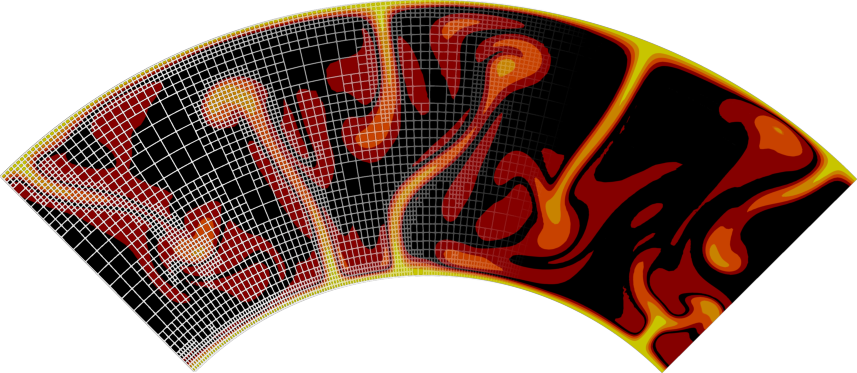
\includegraphics[width=4.5in]{../logo/unlabeled_logo.pdf}
      \hspace{5em}
    \end{center}
  \end{textblock*}

  % Then overlay some text into another textblock* environment that is
  % as wide as the page. We use \raggedright, so everything is shown
  % on the right side of the page. The y-coordinate of the anchor
  % (0.3in) is the same as for the picture, aligning the text nicely
  % to the image.
  \begin{textblock*}{\textwidth}(0in,0.3in)
    \vspace{1em}
    \color{dark_grey}
    \hfill{\Huge \fontfamily{\sfdefault}\selectfont User Manual \\
      \raggedleft \huge \fontfamily{\sfdefault}\selectfont Version
      % keep the following line as is so that we can replace this using a script:
2.4.0-pre %VERSION-INFO%
      \\
      \large(generated \today)
      \\[16pt]
        {\Large
          Wolfgang Bangerth \\
          Juliane Dannberg \\
          Menno Fraters \\
          Rene Gassm{\"o}ller \\
          Anne Glerum \\
          Timo Heister \\
          Bob Myhill \\
          John Naliboff\\}
    }
  \end{textblock*}
}


%AUTHOR(S) & WEBSITE%
\null
\vfill
\color{dark_grey}
{\fontfamily{\sfdefault}\selectfont
% FILL: author list
% e.g. Author One\\Author Two\\Author Three\\
% be sure to have a newline (\\) after the final author
\large
\noindent with contributions by: \\
    Jacqueline Austermann,
    Magali Billen,
    Markus B{\"u}rg,
    Thomas Clevenger,
    Samuel Cox,
    William Durkin,
    Grant Euen,
    Thomas Geenen,
    Ryan Grove,
    Eric Heien,
    Ludovic Jeanniot,
    Louise Kellogg,
    Scott King,
    Martin Kronbichler,
    Marine Lasbleis,
    Haoyuan Li,
    Shangxin Liu,
    Hannah Mark,
    Elvira Mulyukova,
    Bart Niday,
    Jonathan Perry-Houts,
    Elbridge Gerry Puckett,
    Tahiry Rajaonarison,
    Fred Richards,
    Jonathan Robey,
    Ian Rose,
    Max Rudolph,
    Stephanie Sparks,
    D.~Sarah Stamps,
    Cedric Thieulot,
    Wanying Wang,
    Iris van Zelst,
    Siqi Zhang\\
\vspace{0.5em}
}

{\noindent
{\fontfamily{\sfdefault}\selectfont \href{https://geodynamics.org}{geodynamics.org}}
}

%LINE%
{\noindent
\color{dark_grey}
\rule{\textwidth}{2pt}
}

}

\pagebreak
\pagenumbering{arabic}

%%%%%%%%%%%%%%%%%%%%%%%%%%%%%%
%%%   END OF CIG MANUAL COVER TEMPLATE    %%%
%%%%%%%%%%%%%%%%%%%%%%%%%%%%%%

\pagebreak

\tableofcontents

\pagebreak

\section{Introduction}

\aspect{} --- short for Advanced Solver for Problems in Earth's ConvecTion ---
is a code intended to solve the equations that describe thermally driven
convection with a focus on doing so in the context of convection in the Earth
mantle. It is developed by computational scientists all over the world
based on the following principles:
\begin{itemize}
\item \textit{Usability and extensibility:} Simulating mantle convection is a
  difficult problem characterized not only by complicated and nonlinear
  material models but, more generally, by a lack of understanding which parts
  of a much more complicated model are really necessary to simulate the
  defining features of the problem. To name just a few examples:
  \begin{itemize}
  \item Mantle convection is often solved in a spherical shell geometry, but
    the Earth is not a sphere -- its true shape on the longest length scales is
    dominated by polar oblateness, but deviations from spherical shape
    relevant to convection patterns may go down to the length scales of
    mountain belts, mid-ocean ridges or subduction trenches. Furthermore,
    processes outside the mantle like crustal depression during glaciations
    can change the geometry as well.
  \item Rocks in the mantle flow on long time scales, but on shorter time
    scales they behave more like a visco-elasto-plastic material as they break
    and as their crystalline structure heals again. The mathematical models
    discussed in Section~\ref{sec:models} can therefore only be
    approximations.
    \item If pressures are low and temperatures high enough, rocks melt,
      leading to all sorts of new and interesting behavior.
  \end{itemize}
  This uncertainty in what problem one actually wants to solve requires a code
  that is easy to extend by users to support the community in determining what
  the essential features of convection in the Earth mantle are. Achieving this
  goal also opens up possibilities outside the original scope, such as the
  simulation of convection in exoplanets or the icy satellites of the gas
  giant planets in our solar system.

\item \textit{Modern numerical methods:} We build \aspect{} on numerical
  methods that are at the forefront of research in all areas -- adaptive mesh
  refinement, linear and nonlinear solvers, stabilization of
  transport-dominated processes. This implies complexity in our algorithms,
  but also guarantees highly accurate solutions while remaining efficient in
  the number of unknowns and with CPU and memory resources.

\item \textit{Parallelism:} Many convection processes of interest are
  characterized by small features in large domains -- for example, mantle
  plumes of a few tens of kilometers diameter in a mantle almost 3,000 km
  deep. Such problems can not be solved on a single computer but require
  dozens or hundreds of processors to work together. \aspect{} is designed
  from the start to support this level of parallelism.

\item \textit{Building on others' work:} Building a code that satisfies above
  criteria from scratch would likely require several 100,000 lines of
  code. This is outside what any one group can achieve on academic time
  scales. Fortunately, most of the functionality we need is already available
  in the form of widely used, actively maintained, and well tested and
  documented libraries, and we leverage these to make \aspect{} a much smaller
  and easier to understand system. Specifically, \aspect{} builds immediately
  on top of the \dealii{} library (see \url{https://www.dealii.org/}) for
  everything that has to do with finite elements, geometries, meshes, etc.;
  and, through \dealii{} on Trilinos (see \url{http://trilinos.org/})
  for parallel linear algebra and on \pfrst{} (see
  \url{http://www.p4est.org/}) for parallel mesh handling.

\item \textit{Community:} We believe that a large project like \aspect{} can
  only be successful as a community project. Every contribution is welcome and
  we want to help you so we can improve \aspect{} together.

\end{itemize}

Combining all of these aspects into one code makes for an interesting
challenge. We hope to have achieved our goal of providing a useful tool to the
geodynamics community and beyond!


\note{\aspect{} is a community project. As such, we encourage contributions
  from the community to improve this code over time. Natural candidates for
  such contributions are implementations of new plugins as discussed in
  Section~\ref{sec:plugins-concrete} since they are typically self-contained and do not
  require much knowledge of the details of the remaining code. Obviously,
  however, we also encourage contributions to the core functionality in any
  form! If you have something that might be of general interest, please
  contact us.}

\note{\aspect{} will only solve problems relevant to the community if we get
  feedback from the community on things that are missing or necessary for what
  you want to do. Let us know by personal email to the developers, or open
  a topic on our forum hosted at
  \url{https://community.geodynamics.org/c/aspect}!}

\subsection{Referencing \aspect{}}

As with all scientific work, funding agencies have a reasonable expectation
that if we ask for continued funding for this work, we need to demonstrate
relevance.
In addition, many have contributed to the development of \aspect{} and deserve credit
for their work.
To this end, we ask that you cite the appropriate references if you
publish results that were obtained to some part using \aspect{}. For
what exactly to cite and suggestions for acknowledgments,
please see
{\bf \url{https://aspect.geodynamics.org/cite.html}}.

Also see \cite{aspect-doi-v1.5.0,aspect-doi-v2.0.0,aspect-doi-v2.0.1,aspectmanual,KHB12,heister_aspect_methods2}.


\subsection{Acknowledgments}

The development of \aspect{} has been funded
through a variety of grants to the authors. Most immediately, it has been
supported through the Computational Infrastructure in Geodynamics
(CIG), initially by the CIG-I grant (National Science Foundation Award No. EAR-0426271,
via The California Institute of Technology) and later by the CIG-II
and CIG-III grants
(National Science Foundation Awards No. EAR-0949446 and EAR-1550901, via The University
of California -- Davis). In addition, the libraries upon
which \aspect{} builds heavily have been supported through many other grants
that are equally gratefully acknowledged.

Please acknowledge CIG as follows:
{\parindent0pt
  \begin{center}
    \shadowbox{
      \begin{minipage}[c]{0.9\linewidth}
ASPECT is hosted by the Computational Infrastructure for Geodynamics (CIG)
which is supported by the National Science Foundation award EAR-1550901.
      \end{minipage}
    }
  \end{center}
}

The \aspect{} community as a whole, and a number of the primary
developers in particular, owe great thanks to Louise Kellogg
who, when she was the head of CIG, was a strong supporter of the
\aspect{} project. Louise loved how collaborative the \aspect{}
development model was, and how many people contributed. Louise passed
away far too early in 2019, but her support lives on in the spirit of
this project.


\section{Geodynamic modeling assumptions and numerical methods in \aspect{}}
\label{sec:models}

\subsection{Basic equations}
\label{sec:equations}

\aspect{} solves a system of equations in a $d=2$- or $d=3$-dimensional
domain $\Omega$ that describes the motion of a highly viscous fluid driven
by differences in the gravitational force due to a density that depends on
the temperature. In the following, we largely follow the exposition of this
material in Schubert, Turcotte and Olson \cite{STO01}.

Specifically, we consider the following set of equations for velocity $\mathbf
u$, pressure $p$ and temperature $T$, as well as a set of advected quantities
$c_i$ that we call \textit{compositional fields}:
\begin{align}
  \label{eq:stokes-1}
  -\nabla \cdot \left[2\eta \left(\varepsilon(\mathbf u)
                                  - \frac{1}{3}(\nabla \cdot \mathbf u)\mathbf 1\right)
                \right] + \nabla p &=
  \rho \mathbf g
  &
  & \textrm{in $\Omega$},
  \\
  \label{eq:stokes-2}
  \nabla \cdot (\rho \mathbf u) &= 0
  &
  & \textrm{in $\Omega$},
  \\
  \label{eq:temperature}
  \rho C_p \left(\frac{\partial T}{\partial t} + \mathbf u\cdot\nabla T\right)
  - \nabla\cdot k\nabla T
  &=
  \rho H
  \notag
  \\
  &\quad
  +
  2\eta
  \left(\varepsilon(\mathbf u) - \frac{1}{3}(\nabla \cdot \mathbf u)\mathbf 1\right)
  :
  \left(\varepsilon(\mathbf u) - \frac{1}{3}(\nabla \cdot \mathbf u)\mathbf 1\right)
  \\
  &\quad
  +\alpha T \left( \mathbf u \cdot \nabla p \right)
  \notag
  \\
  &\quad
  + \rho T \Delta S \left(\frac{\partial X}{\partial t} + \mathbf u\cdot\nabla X\right)
  &
  & \textrm{in $\Omega$},
  \notag
  \\
  \label{eq:compositional}
  \frac{\partial c_i}{\partial t} + \mathbf u\cdot\nabla c_i
  &=
  q_i
  &
  & \textrm{in $\Omega$},
  i=1\ldots C
\end{align}
where $\varepsilon(\mathbf u) = \frac{1}{2}(\nabla \mathbf u + \nabla\mathbf
u^T)$ is the symmetric gradient of the velocity (often called the
\textit{strain rate}).%
\footnote{There is no consensus in the sciences on the notation used
  for strain and strain rate. The symbols $\varepsilon$,
  $\dot\varepsilon$,  $\varepsilon(\mathbf u)$, and
  $\dot\varepsilon(\mathbf u)$, can all be found. In this manual, and
  in the code, we will consistently use $\varepsilon$ as an
  \textit{operator}, i.e., the symbol is not used on its own but only
  as applied to a field. In other words, if $\mathbf u$ is the
  velocity field, then $\varepsilon(\mathbf u) = \frac{1}{2}(\nabla
  \mathbf u + \nabla\mathbf u^T)$ will denote the strain rate. On the
  other hand, if $\mathbf d$ is the
  displacement field, then $\varepsilon(\mathbf d) = \frac{1}{2}(\nabla
  \mathbf d + \nabla\mathbf d^T)$ will denote the strain.}


In this set of equations, \eqref{eq:stokes-1} and \eqref{eq:stokes-2}
represent the compressible Stokes equations in which $\mathbf u=\mathbf
u(\mathbf x,t)$ is the velocity field and $p=p(\mathbf x,t)$ the pressure
field. Both fields depend on space $\mathbf x$ and time $t$. Fluid flow is
driven by the gravity force that acts on the fluid and that is proportional to
both the density of the fluid and the strength of the gravitational pull.

Coupled to this Stokes system is equation \eqref{eq:temperature} for the
temperature field $T=T(\mathbf x,t)$ that contains heat conduction terms as
well as advection with the flow velocity $\mathbf u$. The right hand side
terms of this equation correspond to
\begin{itemize}
\item internal heat production for example due to radioactive
  decay;
\item friction heating;
\item adiabatic compression of material;
\item phase change.
\end{itemize}
The last term of the temperature equation corresponds to
the latent heat generated or consumed in the process of phase change of material. The latent heat release
is proportional to changes in the fraction of material $X$ that has already
undergone the phase transition (also called phase function) and the change
of entropy $\Delta S$. This process applies both
to solid-state phase transitions and to melting/solidification.
Here, $\Delta S$ is positive for exothermic phase
transitions. As the phase of the material, for a given composition, depends
on the temperature and pressure, the latent heat term can be reformulated:
\begin{gather*}
\frac{\partial X}{\partial t} + \mathbf u\cdot\nabla X
=
\frac{DX}{Dt}
=
\frac{\partial X}{\partial T} \frac{DT}{Dt}
 + \frac{\partial X}{\partial p} \frac{Dp}{Dt}
=
\frac{\partial X}{\partial T}
\left(\frac{\partial T}{\partial t} + \mathbf u\cdot\nabla T
\right)
 + \frac{\partial X}{\partial p} \mathbf u\cdot\nabla p.
\end{gather*}
The last transformation results from the assumption that the flow field is
always in equilibrium and consequently $\partial p/\partial t=0$ (this is the
same assumption that underlies the fact that equation \eqref{eq:stokes-1}
does not have a term $\partial \mathbf u / \partial t$). With this
reformulation, we can rewrite \eqref{eq:temperature} in the following way in
which it is in fact implemented:
\begin{align}
  \label{eq:temperature-reformulated}
  \left(\rho C_p - \rho T \Delta S \frac{\partial X}{\partial T}\right)
  \left(\frac{\partial T}{\partial t} + \mathbf u\cdot\nabla
  T\right) - \nabla\cdot k\nabla T
  &=
  \rho H
  \notag
  \\
  &\quad
  +
  2\eta
  \left(\varepsilon(\mathbf u) - \frac{1}{3}(\nabla \cdot \mathbf u)\mathbf 1\right)
  :
  \left(\varepsilon(\mathbf u) - \frac{1}{3}(\nabla \cdot \mathbf u)\mathbf 1\right)
  \\
  &\quad
  +\alpha T \left( \mathbf u \cdot \nabla p \right)
  \notag
  \\
  &\quad
  + \rho T \Delta S \frac{\partial X}{\partial p} \mathbf u\cdot\nabla p
  & \quad & \textrm{in $\Omega$}.
  \notag
\end{align}

The last of the equations above, equation~\eqref{eq:compositional}, describes
the evolution of additional fields that are transported along with the
velocity field $\mathbf u$ and may react with each other and react to other
features of the solution, but that do not diffuse. We call these fields $c_i$
\textit{compositional fields}, although they can also be used for other
purposes than just tracking chemical compositions. We will discuss this
equation in more detail in Section~\ref{sec:compositional}.

\subsubsection{A comment on adiabatic heating}
Other codes and texts sometimes make a simplification to the adiabatic heating
term in the previous equation. If you assume the vertical component of the
gradient of the \textit{dynamic} pressure to be small compared to the gradient
of the \textit{total} pressure (in other words, the gradient is dominated by
the gradient of the hydrostatic pressure), then $ -\rho \mathbf g \approx
\nabla \mathbf{p} $, and we have the following relation (the negative sign is
due to $\mathbf g$ pointing downwards)
\begin{align*}
\alpha T \left( \mathbf u \cdot \nabla \mathbf p \right)
  & \approx -\alpha \rho T \mathbf u \cdot \mathbf g.
\end{align*}
While this simplification is possible, it is not necessary if you have access
to the total pressure. \aspect{} therefore by default implements the original
term without this simplification, but allows to simplify this term by setting
the ``\texttt{Use simplified adiabatic heating}''
\index[prmindex]{Use simplified adiabatic heating}
\index[prmindexfull]{Heating model!Adiabatic heating!Use simplified adiabatic heating}
parameter in section~\ref{parameters:Heating_20model/Adiabatic_20heating}.

\subsubsection{Boundary conditions}
Having discussed \eqref{eq:temperature}, let us come to the last one of the
original set of equations, \eqref{eq:compositional}. It describes the
motion of a set of advected quantities $c_i(\mathbf x,t),i=1\ldots C$. We call these
\textit{compositional fields} because we think of them as spatially and
temporally varying concentrations of different elements, minerals, or other
constituents of the composition of the material that convects. As such, these
fields participate actively in determining the values of the various
coefficients of these equations. On the other hand, \aspect{} also allows the
definition of material models that are independent of these compositional
fields, making them passively advected quantities. Several of the cookbooks in
Section~\ref{sec:cookbooks} consider compositional fields in this way, i.e.,
essentially as tracer quantities that only keep track of where material came
from.

These equations are
augmented by boundary conditions that can either be of Dirichlet, Neumann, or
tangential type on subsets of the boundary $\Gamma=\partial\Omega$:
\begin{align}
  \mathbf u &= 0 & \qquad &\textrm{on $\Gamma_{0,\mathbf u}$},
  \\
  \mathbf u &= \mathbf u_{\text{prescribed}} & \qquad &\textrm{on
  $\Gamma_{\text{prescribed},\mathbf u}$},
  \\
  \mathbf n \cdot \mathbf u &= 0 & \qquad &\textrm{on $\Gamma_{\parallel,\mathbf
  u}$},
  \\
  (2\eta \varepsilon(\mathbf u) -p I)\mathbf n  &= \mathbf t & \qquad
  &\textrm{on $\Gamma_{\text{traction},\mathbf u}$},
  \\
  T &= T_{\text{prescribed}}
   & \qquad &\textrm{on $\Gamma_{D,T}$},
  \\
  \mathbf n \cdot k\nabla T &= 0
   & \qquad &\textrm{on $\Gamma_{N,T}$}.
  \\
  \label{eq:gamma-in-composition}
  c_i &= c_{i,\text{prescribed}}
   & \qquad &\textrm{on $\Gamma_{\text{in}}=\{\mathbf x: \mathbf
   u\cdot\mathbf n<0\}$}.
\end{align}
Here, the boundary conditions for velocity and temperature are subdivided into
disjoint parts:
\begin{itemize}
  \item $\Gamma_{0,\mathbf u}$ corresponds to parts of the boundary on
which the velocity is fixed to be zero.
  \item $\Gamma_{\text{prescribed},\mathbf u}$ corresponds to parts of the
  boundary on which the velocity is prescribed to some value (which could also
  be zero). It is possible to restrict prescribing the velocity to only certain
  components of the velocity vector.
  \item $\Gamma_{\parallel,\mathbf u}$ corresponds to parts of the boundary on
  which the velocity may be nonzero but must be parallel to the boundary, with the
tangential component undetermined.
  \item $\Gamma_{\text{traction},\mathbf u}$ corresponds to parts of the
  boundary on which the traction is prescribed to some surface force density (a
  common application being $\mathbf t=-p\mathbf n$ if one
  just wants to prescribe a pressure component). It is possible to restrict
  prescribing the traction to only certain vector components.
  \item $\Gamma_{D,T}$ corresponds to places where the temperature is prescribed
  (for example at the inner and outer boundaries of the Earth's mantle).
  \item $\Gamma_{N,T}$ corresponds to places where the temperature is unknown
  but the heat flux across the boundary is zero (for example on symmetry surfaces if only a part
of the shell that constitutes the domain the Earth's mantle occupies is
simulated).
\end{itemize}
We require that one of these boundary conditions hold at each
point for both velocity and temperature, i.e.,
$\Gamma_{0,\mathbf u}\cup\Gamma_{{\text{prescribed}}\mathbf
  u}\cup\Gamma_{\parallel,\mathbf u}\cup\Gamma_{{\text{traction}}\mathbf
  u}=\Gamma$ and
$\Gamma_{D,T}\cup\Gamma_{N,T}=\Gamma$.

Boundary conditions have to be imposed for the compositional fields only
at those parts of the boundary where flow points inward, see equation
\eqref{eq:gamma-in-composition}, but not where it is either tangential
to the boundary or points outward. The difference in treatment between
temperature and compositional boundary conditions is due to the fact
that the temperature equation contains a (possibly small) diffusion
component, whereas the compositional equations do not.

There are other equations that \aspect{} can optionally solve. For example, it
can deal with free surfaces (see Section~\ref{sec:freesurface}), melt generation and
transport (see Section~\ref{sec:melt_transport}), and it can advect along
particles (see Section~\ref{sec:particles}). These optional models
are discussed in more detail in the indicated sections.


\subsubsection{Two-dimensional models}
\label{sec:meaning-of-2d}
\aspect{} allows solving both two- and three-dimensional
models via a parameter in the input files, see also Section~\ref{sec:2d-vs-3d}.
\index[prmindex]{Dimension} \index[prmindexfull]{Dimension}
At the same time, the world is unambiguously three-dimensional. This raises the
question what exactly we mean when we say that we want to solve two-dimensional
problems.

The notion we adopt here -- in agreement with that chosen by many other codes --
is to think of two-dimensional models in the following way: We assume that the
domain we want to solve on is a two-dimensional cross section (parameterized by
$x$ and $y$ coordinates) that extends infinitely far in both negative and
positive $z$ direction. Further, we assume that the velocity is zero in $z$
direction and that all variables have no variation in $z$ direction. As a
consequence, we ought to really think of these two-dimensional models as
three-dimensional ones in which the $z$ component of the velocity is zero and so
are all $z$ derivatives.

If one adopts this point of view, the Stokes equations
\eqref{eq:stokes-1}--\eqref{eq:stokes-2} naturally simplify in a way that allows
us to reduce the $3+1$ equations to only $2+1$, but it makes clear that the
correct description of the compressible strain rate is still
$\varepsilon(\mathbf u) - \frac{1}{3}(\nabla \cdot \mathbf u)\mathbf 1$, rather
than using a factor of $\frac{1}{2}$ for the second term. (A derivation of why
the compressible strain rate tensor has this form can be found in \cite[Section
6.5]{STO01}.)

It is interesting to realize that this compressible strain rate indeed requires
a $3\times 3$ tensor: While under the assumptions above we have
\begin{align*}
  \varepsilon(\mathbf u) =
  \begin{pmatrix}
    \tfrac{\partial u_x}{\partial x}
    &
    \tfrac 12 \tfrac{\partial u_x}{\partial y} +
    \tfrac 12 \tfrac{\partial u_y}{\partial x}
    &
    0
    \\
    \tfrac 12 \tfrac{\partial u_x}{\partial y} +
    \tfrac 12 \tfrac{\partial u_y}{\partial x}
    &
    \tfrac{\partial u_y}{\partial y}
    &
    0
    \\
    0 & 0 & 0
  \end{pmatrix}
\end{align*}
with the expected zeros in the last row and column, the full compressible strain
rate tensor reads
\begin{align*}
  \varepsilon(\mathbf u) - \frac{1}{3}(\nabla \cdot \mathbf u)\mathbf 1 =
  \begin{pmatrix}
    \tfrac 23 \tfrac{\partial u_x}{\partial x}
    - \tfrac 13 \tfrac{\partial u_y}{\partial y}
    &
    \tfrac 12 \tfrac{\partial u_x}{\partial y} +
    \tfrac 12 \tfrac{\partial u_y}{\partial x}
    &
    0
    \\
    \tfrac 12 \tfrac{\partial u_x}{\partial y} +
    \tfrac 12 \tfrac{\partial u_y}{\partial x}
    &
    \tfrac 23 \tfrac{\partial u_y}{\partial y}
    - \tfrac 13 \tfrac{\partial u_x}{\partial x}
    &
    0
    \\
    0 & 0 &
    - \tfrac 13 \tfrac{\partial u_y}{\partial y}
    - \tfrac 13 \tfrac{\partial u_x}{\partial x}
  \end{pmatrix}.
\end{align*}
The entry in the $(3,3)$ position of this tensor may be surprising. It
disappears, however, when taking the (three-dimensional) divergence of the
stress, as is done in \eqref{eq:stokes-1}, because the divergence applies the $z$ derivative to all
elements of the last row -- and the assumption above was that all $z$
derivatives are zero; consequently whatever lives in the third row of the
strain rate tensor does not matter.



\subsubsection{Comments on the final set of equations}
\aspect{} solves these equations in essentially the form stated. In
particular, the form given in \eqref{eq:stokes-1} implies that the pressure
$p$ we compute is in fact the \textit{total pressure}, i.e., the sum of
hydrostatic pressure and dynamic pressure (however, see
Section~\ref{sec:pressure-static-dyn} for more information on this, as well as
the extensive discussion of this issue in \cite{KHB12}).
Consequently, it allows the direct use of this pressure when looking up
pressure dependent material parameters.


\subsection{Coefficients}
\label{sec:coefficients}

The equations above contain a significant number of coefficients that we will
discuss in the following. In the most general form, many of these coefficients
depend nonlinearly on the solution variables pressure $p$, temperature $T$
and, in the case of the viscosity, on the strain rate $\varepsilon(\mathbf
u)$. If compositional fields $\mathfrak c=\{c_1,\ldots,c_C\}$ are present (i.e.,
if $C>0$), coefficients may also depend on them. Alternatively, they may be
parameterized as a function
of the spatial variable $\mathbf x$. \aspect{} allows both kinds of
parameterizations.

Note that below we will discuss examples of the dependence of coefficients on
other quantities; which dependence is actually implemented in the code is a
different matter. As we will discuss in Sections~\ref{sec:parameters} and
\ref{sec:extending}, some versions of these models are already implemented and
can be selected from the input parameter file; others are easy to add to
\aspect{} by providing self-contained descriptions of a set of coefficients
that the rest of the code can then use without a need for further
modifications.

Concretely, we consider the following coefficients and dependencies:
\begin{itemize}
\item \textit{The viscosity $\eta=\eta(p,T,\varepsilon(\mathbf u),\mathfrak
c,\mathbf x)$:} Units $\si{Pa . s} =
  \si{kg}\frac{1}{\si{m . s}}$.

  The viscosity is the proportionality factor that relates total forces
  (external gravity minus pressure gradients) and fluid velocities $\mathbf
  u$. The simplest models assume that $\eta$ is constant, with the constant
  often chosen to be on the order of $10^{21} \si{Pa . s}$.

  More complex (and more realistic) models assume that the viscosity depends
  on pressure, temperature and strain rate. Since this dependence is often
  difficult to quantify, one modeling approach is to make $\eta$ spatially
  dependent.

\item \textit{The density $\rho=\rho(p,T,\mathfrak c,\mathbf x)$:} Units
  $\frac{\si{kg}}{\si{m}^3}$.

  In general, the density depends on pressure and temperature, both through
  pressure compression, thermal expansion, and phase changes the material may
  undergo as it moves through the pressure-temperature phase diagram.

  The simplest parameterization for the density is to assume a linear
  dependence on temperature, yielding the form
  $\rho(T)=\rho_{\text{ref}}[1-\alpha (T-T_{\text{ref}})]$ where
  $\rho_{\text{ref}}$ is the reference density at temperature $T_{\text{ref}}$
  and $\alpha$ is the linear thermal expansion coefficient. For the earth's
  mantle, typical values for this parameterization would be
  $\rho_{\text{ref}}=3300\frac{\si{kg}}{\si{m}^3}$,
  $T_{\text{ref}}=293 \si{K}$, $\alpha=\num{2e-5}
  \frac{1}{\mathrm{K}}$.

\item \textit{The gravity vector $\mathbf g=\mathbf g(\mathbf x)$:} Units
  $\frac{\si{m}}{\textrm{s}^2}$.

  Simple models assume a radially inward gravity vector of constant magnitude
  (e.g., the surface gravity of Earth, $9.81 \frac{\si{m}}{\textrm{s}^2}$),
  or one that can be computed analytically assuming a homogeneous mantle
  density.

  A physically self-consistent model would compute the gravity vector as
  $\mathbf g = -\nabla \varphi$ with a gravity potential $\varphi$ that
  satisfies $-\Delta\varphi=4\pi G\rho$ with the density $\rho$ from above and
  $G$ the universal constant of gravity. This would provide a gravity vector
  that changes as a function of time. Such a model is not currently
  implemented.

\item \textit{The specific isobaric heat capacity $C_p=C_p(p,T,\mathfrak c,\mathbf x)$:}
Units \si{J/kg/K} = \si{m^2/s^2/K}.

  The specific heat capacity denotes the amount of energy needed to increase
  the temperature of one kilogram of material by one Kelvin at constant pressure.
  Wikipedia lists a value of
  $790 \si{J/kg/K}$ for granite%
  \footnote{See \url{http://en.wikipedia.org/wiki/Specific_heat}.}
  For the Earth's mantle, a value of $1250
  \si{J/kg/K}$ is within the range
  suggested by the literature.


\item \textit{The thermal conductivity $k=k(p,T,\mathfrak c,\mathbf x)$:} Units
  $\frac{\textrm{W}}{\si{m}\cdot\si{K}}=\frac{\si{kg}\cdot\si{m}}{\textrm{s}^3\cdot\si{K}}$.

  The thermal conductivity denotes the amount of thermal energy flowing
  through a unit area for a given temperature gradient. It depends on the
  material and as such will from a physical perspective depend on pressure and
  temperature due to phase changes of the material as well as through
  different mechanisms for heat transport (see, for example, the partial
  transparency of perovskite, the most abundant
  material in the earth mantle, at pressures above around 120 GPa
  \cite{BRVMFG04}).

  As a rule of thumb for its
  order of magnitude, Wikipedia quotes values of
  $1.83$--$2.90\frac{\textrm{W}}{\si{m}\cdot\si{K}}$ for sandstone and
  $1.73$--$3.98\frac{\textrm{W}}{\si{m}\cdot\si{K}}$ for granite.%
  \footnote{See \url{http://en.wikipedia.org/wiki/Thermal_conductivity} and
    \url{http://en.wikipedia.org/wiki/List_of_thermal_conductivities}.} The
  values in the mantle are almost certainly higher than this though probably
  not by much. The exact value is not really all that important: heat
  transport through convection is several orders of magnitude more important
  than through thermal conduction.

  The thermal conductivity $k$ is often expressed in terms of the
  \textit{thermal diffusivity} $\kappa$ using the relation $k = \rho C_p \kappa$.

\item \textit{The intrinsic specific heat production $H=H(\mathbf x)$:} Units
  $\frac{\textrm{W}}{\si{kg}}=\frac{\si{m}^2}{\textrm{s}^3}$.

  This term denotes the intrinsic heating of the material, for example due to
  the decay of radioactive material. As such, it depends not on pressure or
  temperature, but may depend on the location due to different chemical
  composition of material in the earth mantle. The literature suggests a value
  of $\gamma=\num{7.4e-12}\frac{\textrm{W}}{\si{kg}}$.

\item \textit{The thermal expansion coefficient $\alpha=\alpha(p,T,\mathfrak c ,\mathbf x)$:} Units
  $\frac{1}{\si{K}}$.

  This term denotes by how much the material under consideration
  expands due to temperature increases at constant pressure.
  This coefficient is defined as
  $\alpha = -\frac{1}{\rho} \left(\frac{\partial \rho}{\partial T}\right)_{p}$,
  where the negative sign is due the fact that the density
  \textit{decreases} as a function of temperature. Alternatively, if
  one considers the \textit{volume} $V=V(T)$ a piece of material of mass $M$
  occupies, $V=\frac{M}{\rho}$, then the thermal expansion coefficient
  is defined as the relative increase in volume,
  $\alpha=\frac{1}{V}\frac{\partial V(T)}{\partial T}$, because
  $\frac{\partial V(T)}{\partial T} =
   \frac{\partial \frac{M}{\rho}}{\partial T} =
   -\frac{M}{\rho^2} \frac{\partial \rho}{\partial T} =
   -\frac{V}{\rho} \frac{\partial \rho}{\partial T}$.

   The literature suggests that values of $\alpha=\num{1e-5}\frac{1}{\si{K}}$ at the core-mantle boundary and $\alpha=\num{4e-5}\frac{1}{\si{K}}$ are appropriate for Earth.

\item \textit{The isothermal compressibility $\beta_T=\beta_T(p,T,\mathfrak c ,\mathbf x)$:} Units
  $\frac{1}{\textrm{Pa}}$.

  This term quantifies how much the material under consideration
  contracts due to pressure increases at constant temperature.
  This coefficient is defined as
  $\beta_T = \frac{1}{\rho} \left( \frac{\partial \rho}{\partial p} \right)_{T}$.
  Alternatively, if
  one considers the \textit{volume} $V=V(p, T)$ a piece of material of mass $M$
  occupies, $V=\frac{M}{\rho}$, then the isothermal compressibility
  is defined as the relative increase in volume,
  $\beta=\frac{1}{V}\left(\frac{\partial V(p, T)}{\partial p}\right)_{T}$, because
  $\frac{\partial V(p, T)}{\partial p} =
   \frac{\partial \frac{M}{\rho}}{\partial p} =
   -\frac{M}{\rho^2} \frac{\partial \rho}{\partial p} =
   -\frac{V}{\rho} \frac{\partial \rho}{\partial p}$.

   Values of $\beta=10^{-12}$ -- $10^{-11} \frac{1}{\textrm{Pa}}$
   are reasonable for Earth's mantle, with values decreasing by about a factor of 5 between the shallow lithosphere and core-mantle boundary.

\item \textit{The isentropic/adiabatic compressibility $\beta_S=\beta_S(p,T,\mathfrak c ,\mathbf x)$:} Units
  $\frac{1}{\textrm{Pa}}$.

  This term quantifies how much the material under consideration
  contracts due to pressure increases at constant entropy.
  This coefficient is defined as
  $\beta_S = \frac{1}{\rho} \left( \frac{\partial \rho}{\partial p} \right)_{S}$.
  Alternatively, if
  one considers the \textit{volume} $V=V(p, T)$ a piece of material of mass $M$
  occupies, $V=\frac{M}{\rho}$, then the isentropic compressibility
  is defined as the relative increase in volume,
  $\beta=\frac{1}{V}\left(\frac{\partial V(p, T)}{\partial p}\right)_{S}$, because
  $\frac{\partial V(p, T)}{\partial p} =
   \frac{\partial \frac{M}{\rho}}{\partial p} =
   -\frac{M}{\rho^2} \frac{\partial \rho}{\partial p} =
   -\frac{V}{\rho} \frac{\partial \rho}{\partial p}$.
   The isentropic and isothermal compressibility are related by the expression:
   \begin{equation}
     \beta_S = \beta_T - \frac{\alpha^2 T}{\rho C_p}
   \end{equation}
   The ratio of the compressibilities decreases with increasing temperature
   and increases with increasing pressure. In the Earth's convecting mantle,
   $\beta_S/\beta_T = 0.92$--$0.98$. Different mineral assemblages have
   different values of this ratio under the same conditions. For example, the
   upper-lower boundary may exhibit a 3--4\% drop in $\beta_S / \beta_T$
   as a result of a 40\% lower $C_p$ of bridgmanite-periclase assemblages
   relative to the olivine polymorphs.


\item \textit{The change in entropy $\Delta S$ at a
  phase transition together with the derivatives of the phase function
  $X=X(p,T,\mathfrak c,\mathbf x)$ with regard to temperature and pressure:} Units
  \si{J/kg/K^2} ($-\Delta S \frac{\partial X}{\partial T}$) and
  \si{m^3/kg/K} ($\Delta S \frac{\partial X}{\partial p}$).

  When material undergoes a phase transition, the entropy changes due to
  release or consumption of latent heat. However, phase transitions occur
  gradually and for a given chemical composition it depends on temperature
  and pressure which phase prevails. Thus, the latent heat release can
  be calculated from the change of entropy $\Delta S$ and the derivatives
  of the phase function $\frac{\partial X}{\partial T}$ and
  $\frac{\partial X}{\partial p}$. These values have to be provided by
  the material model, separately for the coefficient
  $-\Delta S \frac{\partial X}{\partial T}$ on the left-hand side and
  $\Delta S \frac{\partial X}{\partial p}$ on the right-hand side of the
  temperature equation. However, they may be either approximated with the help
  of an analytic phase function, employing data from a thermodynamic database
  or in any other way that seems appropriate to the user.
\end{itemize}

\subsubsection{Coefficient self-consistency}
\label{sec:coefficient_self_consistency}
\textit{This section was contributed by Bob Myhill.}

The coefficients in the previous section may at first appear independent.
However, there are thermodynamic relations between these properties which must be
satisfied in any self-consistent material model.
The following section describes the relations required for thermodynamic
consistency, and presents some suggested ways by which consistency can be assured.

In order to derive the relationships between different material properties, we must
introduce a thermodynamic potential known as the
\href{https://en.wikipedia.org/wiki/Gibbs_free_energy}{\textit{specific
    Gibbs free energy}}
$\mathcal{G}(p, T)$ with units $\si{J}/\si{kg}$. The word ``specific'' indicates that the energy is
given per unit mass, rather than volume or number of atoms or molecules. This potential is
equal to the maximum amount of non-expansion work that can be extracted from a
thermodynamically closed system. At equilibrium conditions and fixed temperature and
pressure, the Gibbs free energy is minimized. The following equations provide the
definitions and relationships between thermodynamic properties in terms of the specific
Gibbs free energy:
\begin{eqnarray}
  S &=& - \left( \frac{\partial \mathcal{G}}{\partial T} \right)_{p}, \\
  \frac{1}{\rho} &=& \left( \frac{\partial \mathcal{G}}{\partial p} \right)_{T}, \label{eq:mm_density} \\
  \frac{\alpha}{\rho} &=& \frac{\partial^2 \mathcal{G}}{\partial {p} \, \partial {T}}, \label{eq:mm_alpha_g} \\
  \beta_T &=& -\rho \left( \frac{\partial^2 \mathcal{G}}{\partial {p}^2}  \right)_{T}, \label{eq:mm_betaT_g} \\
  C_p &=& -T \left( \frac{\partial^2 \mathcal{G}}{\partial {T}^2}  \right)_{p}, \label{eq:mm_isobaric_heat_capacity} \\
  \beta_S &=& \beta_T - \frac{\alpha^2 T}{\rho C_p}, \label{eq:mm_isentropic_compressibility} \\
  \frac{C_V}{C_p} &=& \frac{\beta_S}{\beta_T}, \\
  \gamma &=& \frac{\alpha }{\beta_T \rho C_V}.
\end{eqnarray}
where $S$ is the specific entropy, $C_p$ and $C_V$ are the specific isobaric
and isochoric heat capacities, $\beta_T$ and $\beta_S$ are the isothermal and isotropic
compressibilities, and $\gamma$ is the thermodynamic Gr\"{u}neisen parameter. The subscript
indicates the thermodynamic variable ($p$ or $T$) that is held constant.

Thermodynamically self-consistent material models must obey the explicit and implicit relations
between the different properties \emph{at all pressures and temperatures}. Explicit relations
are here defined as those between properties and their derivatives, such as that between
density and thermal expansivity. Implicit relations involve mixed pressure and temperature
derivatives, and derive from the symmetry of second derivatives. The following paragraphs
list the relations most relevant for the construction of thermodynamically-consistent material
models in \aspect{}.

\paragraph{Consistency in $\boldsymbol{\rho}$-$\boldsymbol{\alpha}$ and $\boldsymbol{\rho}$-$\boldsymbol{\beta_T}$}
Using the chain rule to combine~\eqref{eq:mm_density},~\eqref{eq:mm_alpha_g}
and~\eqref{eq:mm_betaT_g} yields the more familiar definitions of $\alpha$ and $\beta_T$:
\begin{eqnarray}
  \alpha &=& -\frac{1}{\rho} \left( \frac{\partial \rho}{\partial T} \right)_{p}, \label{eq:mm_thermal_expansivity} \\
  \beta_T &=& \frac{1}{\rho} \left( \frac{\partial \rho}{\partial p} \right)_{T}. \label{eq:mm_isothermal_compressibility}
\end{eqnarray}

\paragraph{Isobaric heat capacity}

We start by taking the partial derivative of the isobaric heat
capacity~\eqref{eq:mm_isobaric_heat_capacity} with respect to pressure at constant temperature:
\begin{eqnarray}
  \left( \frac{\partial C_p}{\partial p} \right)_{T} &=& -T \frac{\partial^3 \mathcal{G}}{\partial {T}^2 \, \partial {p}} \\
  &=& -T \left( \frac{\partial \left(\alpha / \rho \right)}{\partial T} \right)_{p}. \label{eq:heat_capacity_p_dependence}
\end{eqnarray}
From this expression it becomes clear that if $\alpha / \rho$ has any temperature dependence,
the heat capacity $C_p$ \emph{cannot} be globally constant. One way to solve this issue is to define
heat capacity at constant pressure, and then integrate~\eqref{eq:heat_capacity_p_dependence}
with respect to pressure:
\begin{equation}
  C_p(p, T)
  = C_p(p_{\textrm{ref}}, T) -T \int_{p_{\textrm{ref}}}^p
  \left(\frac{\partial \left(\alpha / \rho \right)}{\partial T} \right)_{p}
  \text{d}p.
\end{equation}
There is no guarantee that this expression will have a form for which the integral can be found analytically.

\paragraph{Isentropic gradient}
The material properties also define the slope of the adiabat (the change in temperature with
pressure at constant entropy) at all pressures and temperatures. Using the cyclic relation,
we can define this slope in terms of partial differentials of the entropy with respect to pressure
and temperature:
\begin{eqnarray}
  \left( \frac{\partial T}{\partial p} \right)_{S} &=& - \left( \frac{\partial T}{\partial S} \right)_{p} \left( \frac{\partial S}{\partial p} \right)_{T} \\
  &=& - \left( \frac{T}{C_p} \right) \left( - \frac{\alpha}{\rho} \right) \\
  &=& \frac{\alpha T}{\rho C_p} \label{eq:mm_isentropic_gradient}
\end{eqnarray}
This expression does not pose a constraint on the material properties, but in order to be
self-consistent, the adiabat must be computed following this relation.

For complex material models, obtaining analytical functions which obey all these relations
may be a non-trivial exercise. Furthermore, it is often not immediately clear when a
given formulation is thermodynamically inconsistent. Indeed, both the
thermodynamic and the geodynamic literature contain many equations of
state and material parameterizations which do not obey these
relations! This may not invalidate the results obtained with these
models, but it is a point worth keeping in mind as the geodynamics
community moves to more complicated and more realistic parameterizations.

\emph{A final note of warning: Some compressible formulations in \aspect{}
  (Section~\ref{sec:mass-conservation-approximation}) use the isothermal compressibility,
  while others use the isentropic compressibility. Fully self-consistent material models must
  either specify what approximation of the compressible equations they are consistent with
  (see Section~\ref{sec:approximate-equations}), or have a switch so that they use the correct
  compressibility for each of the different approximations. The conversion between isothermal
  and isentropic compressibilities is given in~\eqref{eq:mm_isentropic_compressibility}.}


\subsubsection{Coefficient averaging}
In multiphase rocks, or multirock areas in convection simulations, properties must be averaged
because the length scales at which the rock types vary is far smaller than the resolution of the mesh.
As a consequence, we need to use ``effective coefficients'', i.e., coefficients that do not
correspond to any particular rock, but that lead to a macroscopic response that is a good match
to the response of the correct, but unresolvable mixture of rocks.
For viscosity and conductivity, there is no single expression that describes how averaging should
be performed; indeed, these properties are dependent on rock texture and mineral alignment,
both of which may change through time as strain accumulates, and chemical diffusion and
reactions take place. Some of the existing multicomponent material models in \aspect{} allow the
user to choose from a range of averaging schemes for viscosity.

In the case of density, thermal expansivity, heat capacity and bulk compressibility, there is
one correct way of averaging. Here we must consider conservation of mass and composition in a
multicomponent rock $r$. If component $i$ has masses $M_i$ and densities $\rho_i$, we
can consider the summation of volume fractions:
\begin{eqnarray}
  V_r &=& \frac{M_r}{\rho_r} = \sum_i \frac{M_i}{\rho_i} \\
  \frac{1}{\rho_r} &=& \sum_i \frac{x_i}{\rho_i}
\end{eqnarray}
where $x_i$ are mass fractions of the components in the rock.

Similarly, we can obtain averaging formulae for the other thermodynamic properties:
\begin{eqnarray}
  \frac{\alpha}{\rho} &=& \sum_i x_i \frac{\alpha_i}{\rho_{i}} \\
  \frac{\beta_T}{\rho} &=& \sum_i x_i \frac{\beta_{Ti}}{\rho_{i}} \\
  C_p &=& \sum_i x_i C_{pi}
\end{eqnarray}



\subsection{Dimensional or non-dimensionalized equations?}
\label{sec:non-dimensional}

Equations \eqref{eq:stokes-1}--\eqref{eq:temperature} are stated in their
physically correct form. One would usually interpret them in a way that the
various coefficients such as the viscosity, density and thermal conductivity
$\eta,\rho,\kappa$ are given in their correct physical units, typically
expressed in a system such as the meter, kilogram, second (MKS) system that is
part of the \href{http://en.wikipedia.org/wiki/SI}{SI} system.
This is certainly how we envision \aspect{} to be used: with geometries,
material models, boundary conditions and initial values to be given in their correct
physical units. As a consequence, when \aspect{} prints information about the
simulation onto the screen, it typically does so by using a postfix such as
\texttt{m/s} to indicate a velocity or \texttt{W/m\^{}2} to indicate a heat
flux.

\note{For mantle convection simulations, it is often convenient to work with
time units of \textit{years} instead of \textit{seconds}. The flag
``\texttt{Use years in output instead of seconds}'' (Section~\ref{parameters:global})
in the input file determines how input and output parameters with units of time or
velocity are interpreted. For details, see Section~\ref{sec:years-or-seconds} below.}

That said, in reality, \aspect{} has no preferred system of
units as long as every material constant, geometry, time, etc., are all
expressed in the same system. In other words, it is entirely legitimate to
implement geometry and material models in which the dimension of the domain is
one, density and viscosity are one, and the density variation as a function of
temperature is scaled by the Rayleigh number -- i.e., to use the usual
non-dimensionalization of the equations~\eqref{eq:stokes-1}--\eqref{eq:temperature}. Some of the cookbooks in
Section~\ref{sec:cookbooks} use this non-dimensional form; for example,
the simplest cookbook in Section~\ref{sec:cookbooks-simple-box} as well as
the SolCx, SolKz and inclusion benchmarks in Sections~\ref{sec:benchmark-solcx},
are such cases. Whenever this is the case, output showing units \texttt{m/s} or
\texttt{W/m\^{}2} clearly no longer have a literal meaning. Rather, the unit postfix must in this case simply
be interpreted to mean that the number that precedes the first is a velocity and
a heat flux in the second case.

In other words, whether a computation uses physical or non-dimensional units
really depends on the geometry, material, initial and boundary condition
description of the particular case under consideration -- \aspect{} will simply
use whatever it is given. Whether one or the other is the more appropriate
description is a decision we purposefully leave to the user. There are of
course good reasons to use non-dimensional descriptions of realistic problems,
rather than to use the original form in which all coefficients remain in their
physical units. On the other hand, there are also downsides:
\begin{itemize}
  \item Non-dimensional descriptions, such as when using the
  \href{http://en.wikipedia.org/wiki/Rayleigh_number}{Rayleigh} number to
  indicate the relative strength of convective to diffusive thermal transport,
  have the advantage that they allow to reduce a system to its essence. For
  example, it is clear that we get the same behavior if one increases both the
  viscosity and the thermal expansion coefficient by a factor of two because the
  resulting Rayleigh number; similarly, if we were to increase the size of the
  domain by a factor of 2 and thermal diffusion coefficient by a factor of 8. In both of
  these cases, the non-dimensional equations are exactly the same. On the other
  hand, the equations in their physical unit form are different and one may not
  see that the result of this variations in coefficients will be exactly the
  same as before. Using non-dimensional variables therefore reduces the space of
  independent parameters one may have to consider when doing parameter studies.

  \item From a practical perspective, equations
  \eqref{eq:stokes-1}--\eqref{eq:temperature} are often ill-conditioned in
  their original form: the two sides of each equation have physical units
  different from those of the other equations, and their numerical values are
  often vastly different.%
  \footnote{To illustrate this, consider convection in the Earth as a
  back-of-the-envelope example.
  With the length scale of the mantle $L=\num{3e6}\;\si{m}$, viscosity
  $\eta=10^{24} \; \si{kg}/\si{m}/\si{s}$, density $\rho=\num{3e3} \; \si{kg}/\si{m}^3$ and a typical
  velocity of $U=0.1\;\si{m}/\text{year}=\num{3e-9}\; \si{m}/\si{s}$, we get that the friction
  term in \eqref{eq:stokes-1} has size $\eta U/L^2 \approx \num{3e2} \;
  \si{kg}/\si{m}^2/\si{s}^2$. On the other hand, the term $\nabla\cdot(\rho u)$ in the
  continuity equation \eqref{eq:stokes-2} has size $\rho U/L\approx \num{3e-12} \; \si{kg}/\si{s}/\si{m}^3$. In other words, their \textit{numerical values} are 14
  orders of magnitude apart.}
  Of course, these values can not be compared: they have different physical
  units, and the ratios between these values depends on whether we choose to
  measure lengths in meters or kilometers, for example. Nevertheless, when
  implementing these equations in software, at one point or another, we have to
  work with numbers and at this point the physical units are lost. If one does
  not take care at this point, it is easy to get software in which all accuracy
  is lost due to round-off errors. On the other hand, non-dimensionalization
  typically avoids this since it normalizes all quantities so that values that
  appear in computations are typically on the order of one.

  \item On the downside, the numbers non-dimensionalized equations produce are
  not immediately comparable to ones we know from physical experiments. This is
  of little concern if all we have to do is convert every output number of our
  program back to physical units. On the other hand, it is more difficult and a
  source of many errors if this has to be done inside the program, for example,
  when looking up the viscosity as a pressure-, temperature- and
  strain-rate-dependent function: one first has to convert pressure,
  temperature and strain rate from non-dimensional to physical units, look up
  the corresponding viscosity in a table, and then convert the viscosity back to
  non-dimensional quantities. Getting this right at every one of the dozens or
  hundreds of places inside a program and using the correct (but distinct)
  conversion factors for each of these quantities is both a challenge and a possible source
  of errors.

  \item From a mathematical viewpoint, it is typically clear how an equation
  needs to be non-dimensionalized if all coefficients are constant. However, how
  is one to normalize the equations if, as is the case in the earth mantle, the
  viscosity varies by several orders of magnitude? In cases like these, one has
  to choose a reference viscosity, density, etc. While the resulting
  non-dimensionalization retains the universality of parameters in the
  equations, as discussed above, it is not entirely clear that this would also
  retain the numerical stability if the reference values are poorly chosen.
\end{itemize}

As a consequence of such considerations, most codes in the past have used
non-dimensionalized models. This was aided by the fact that until recently and
with notable exceptions, many models had constant coefficients and the
difficulties associated with variable coefficients were not a concern. On the
other hand, our goal with \aspect{} is for it to be a code that solves realistic
problems using complex models and that is easy to use. Thus, we allow users to
input models in physical or non-dimensional units, at their discretion. We
believe that this makes the description of realistic models simpler. On
the other hand, ensuring numerical stability is not something users should have
to be concerned about, and is taken care of in the implementation of \aspect{}'s
core (see the corresponding section in \cite{KHB12}).

\subsubsection{Years or seconds?}
\label{sec:years-or-seconds}

All internal calculations in \aspect{} are performed using time units of seconds.
Input quantities with units of time or velocity are assumed to be in
seconds or meters per second, and output quantities with units of time or velocity
will also be in seconds or meters per second, unless the input parameter
\texttt{Use years in output instead of seconds} is \texttt{true}
(see Section~\ref{parameters:global}).

This parameter is somewhat deceptively named, as it influences how \aspect{}
treats inputs as well as outputs. For example, if \texttt{Use years in output instead
of seconds} is \texttt{true}, input values for \texttt{Start time},
\texttt{End time}, and \texttt{Maximum time step} are assumed to be in years
instead of seconds. When the flag is set, \aspect{} converts input time and velocity
units to MKS internally, computes solutions, and converts time and velocity outputs
back to years and meters per year during postprocessing.

By default, \texttt{Use years in output instead of seconds} is \texttt{true},
since \aspect{} is designed primarily for models described in physical units rather
than in non-dimensionalized form, and years are often more intuitive time units
for mantle convection problems (see Section~\ref{sec:non-dimensional}). For non-
dimensional models the flag should be set to \texttt{false} since conversions
between years and seconds do not make sense for non-dimensional quantities.

\subsection{Static or dynamic pressure?}
\label{sec:pressure-static-dyn}

One could reformulate equation \eqref{eq:stokes-1} somewhat. To this end, let us
say that we would want to represent the pressure $p$ as the sum of two parts
that we will call static and dynamic, $p=p_s+p_d$. If we assume that $p_s$ is
already given, then we can replace \eqref{eq:stokes-1} by
\begin{gather*}
  -\nabla \cdot 2\eta
  \nabla \mathbf u + \nabla p_d =
  \rho\mathbf g - \nabla p_s.
\end{gather*}
One typically chooses $p_s$ as the pressure one would get if the whole medium
were at rest -- i.e., as the hydrostatic pressure. This pressure can be
computed noting that \eqref{eq:stokes-1} reduces to
\begin{gather*}
  \nabla p_s = \rho(p_s,T_s,\mathbf x)\mathbf g = \bar\rho \mathbf g
\end{gather*}
in the absence of any motion where $T_s$ is some static temperature field (see
also Section~\ref{sec:adiabatic}). This, our rewritten version of
\eqref{eq:stokes-1} would look like this:
\begin{gather*}
  -\nabla \cdot 2\eta
  \nabla \mathbf u + \nabla p_d =
  \left[\rho(p,T,\mathbf x)-\rho(p_s,T_s,\mathbf x)\right]\mathbf g.
\end{gather*}
In this
formulation, it is clear that the quantity that drives the fluid flow is in
fact the \textit{buoyancy} caused by the \textit{variation} of densities,
not the density itself.

This reformulation has a number of advantages and disadvantages:
\begin{itemize}
\item One can notice that in many realistic cases, the dynamic component $p_d$
  of the pressure is orders of magnitude smaller than the static component
  $p_s$. For example, in the earth, the two are separated by around 6 orders
  of magnitude at the bottom of the earth mantle. Consequently, if one wants
  to solve the linear system that arises from discretization of the original
  equations, one has to solve it a significant degree of accuracy (6--7
  digits) to get the dynamic part of the pressure correct to even one
  digit. This entails a very significant numerical effort, and one that is not
  necessary if we can split the pressure in a way so that the pre-computed
  static pressure $p_s$ (or, rather, the density using the static pressure and
  temperature from which $p_s$ results) absorbs the dominant part and one only
  has to compute the remaining, dynamic pressure to 2 or 3 digits of accuracy,
  rather than the corresponding 7--8 for the total pressure.

\item On the other hand, the pressure $p_d$ one computes this way is not immediately
  comparable to quantities that we use to look up pressure-dependent
  quantities such as the density. Rather, one needs to first find the static
  pressure as well (see Section~\ref{sec:adiabatic}) and add the two together
  before they can be used to look up material properties or to compare them with
  experimental results. Consequently, if the pressure a program outputs
  (either for visualization, or in the internal interfaces to parts of the
  code where users can implement pressure- and temperature-dependent material
  properties) is only the dynamic component, then all of the consumers of this
  information need to convert it into the total pressure when comparing with
  physical experiments. Since any code implementing realistic material models
  has a great many of these places, there is a large potential for inadvertent
  errors and bugs.

\item Finally, the definition of a reference density $\rho(p_s,T_s,\mathbf x)$
  derived from static pressures and temperatures
  is only simple if we have incompressible models and under the assumption
  that the temperature-induced density variations are small compared to the
  overall density. In this case, we can choose $\rho(p_s,T_s,\mathbf
  x)=\rho_0$ with a constant reference density $\rho_0$. On the other hand,
  for more complicated models, it is not a priori
  clear which density to choose since we first need to compute static
  pressures and temperatures -- quantities that satisfy equations that
  introduce boundary layers, may include phase changes releasing latent heat,
  and where the density may have discontinuities at certain depths, see
  Section~\ref{sec:adiabatic}.

  Thus, if we compute adiabatic pressures and
  temperatures $\bar p_s,\bar T_s$ under the assumption of a thermal boundary layer
  worth 900 Kelvin at the top, and we get a corresponding density profile
  $\bar\rho=\rho(\bar p_s,\bar T_s, \mathbf x)$, but after running for a few
  million years the temperature turns out to be so that the top boundary layer
  has a jump of only 800 Kelvin with corresponding adiabatic pressures and
  temperatures $\hat p_s,\hat T_s$, then a more appropriate density profile
  would be $\hat\rho=\rho(\hat p_s,\hat T_s, \mathbf x)$.

  The problem is that it may well be that the erroneously computed density
  profile $\hat \rho$ does \textit{not} lead to a separation where
  $|p_d|\ll|p_s|$ because, especially if the material undergoes phase changes,
  there will be entire areas of the computational domain in which $|\rho-\hat
  \rho_s|\ll |\rho|$ but $|\rho-\bar
  \rho_s|\not\ll |\rho|$. Consequently the benefits of lesser requirements on the
  iterative linear solver would not be realized.
\end{itemize}

We do note that most of the codes available today and that we are aware of
split the pressure into static and dynamic parts nevertheless, either
internally or require the user to specify the density profile as the
difference between the true and the hydrostatic density. This may, in part, be
due to the fact that historically most codes were written to solve problems
in which the medium was considered incompressible, i.e., where the definition
of a static density was simple.

On the other hand, we intend \aspect{} to be a code that can solve more
general models for which this definition is not as simple. As a consequence, we
have chosen to solve the equations as stated originally -- i.e., we solve for
the \textit{full} pressure rather than just its \textit{dynamic} component. With
most traditional methods, this would lead to a catastrophic loss of accuracy in the
dynamic pressure since it is many orders of magnitude smaller than the total
pressure at the bottom of the earth mantle. We avoid this problem in \aspect{}
by using a cleverly chosen iterative solver that ensures that the full pressure
we compute is accurate enough so that the dynamic pressure can be extracted from
it with the same accuracy one would get if one were to solve for only the
dynamic component. The methods that ensure this are described in detail in
\cite{KHB12} and in particular in the appendix of that paper.

\note{By default, \aspect{} uses the full pressure in the equations, and only prescribing
density deviations from a reference state on the right-hand side of \eqref{eq:stokes-1}
would lead to negative densities in the energy equation \eqref{eq:temperature}.
However, when using one of the approximations described in Section \ref{sec:approximate-equations},
the energy balance uses the reference density $\bar\rho$ instead of the full density,
which makes it possible to formulate the Stokes system in terms of the dynamic instead of
the full pressure. In order to do this, one would have to use a material model
(see Section~\ref{sec:material-models}) in which the density is in fact a density variation,
and then the pressure solution variable would only be the dynamic pressure.}

\subsection{Pressure normalization}
\label{sec:pressure}

The equations described above, \eqref{eq:stokes-1}--\eqref{eq:temperature},
only determine the pressure $p$ up to an additive constant. On the other hand,
since the pressure appears in the definition of many of the coefficients, we
need a pressure that has some sort of \textit{absolute} definition. A
physically useful definition would be to normalize the pressure in such a way
that the average pressure along the ``surface'' has a prescribed value where
the geometry description (see Section~\ref{sec:geometry-models}) has to
determine which part of the boundary of the domain is the ``surface'' (we call
a part of the boundary the ``surface'' if its depth is ``close to zero'').

Typically, one will choose this average pressure to be zero, but there is a
parameter ``\texttt{Surface pressure}''
\index[prmindex]{Surface pressure}
\index[prmindexfull]{Surface pressure}
in the input file (see Section~\ref{parameters:global}) to set it to
a different value. One may want to do that, for example, if one wants to
simulate the earth mantle without the overlying lithosphere. In that case, the
``surface'' would be the interface between mantle and lithosphere, and the
average pressure at the surface to which the solution of the equations will be
normalized should in this case be the hydrostatic pressure at the bottom of
the lithosphere.

An alternative is to normalize the pressure in such a way that the
\textit{average} pressure throughout the domain is zero or some constant
value. This is not a useful approach for most geodynamics applications but is
common in benchmarks for which analytic solutions are available. Which kind of
normalization is chosen is determined by the ``\texttt{Pressure
  normalization}'' flag in the input file,
\index[prmindex]{Pressure normalization}
\index[prmindexfull]{Pressure normalization}
see Section~\ref{parameters:global}.


\subsection{Initial conditions and the adiabatic pressure/temperature}
\label{sec:adiabatic}

Equations \eqref{eq:stokes-1}--\eqref{eq:temperature} require us to
pose initial conditions for the temperature, and this is done by
selecting one of the existing models for initial conditions in the
input parameter file, see
Section~\ref{parameters:Initial_20temperature_20model}. The equations
themselves do not require that initial conditions are specified for
the velocity and pressure variables (since there are no time
derivatives on these variables in the model).

Nevertheless, a nonlinear solver will have difficulty converging to
the correct solution if we start with a completely unphysical pressure
for models in which coefficients such as density $\rho$ and viscosity
$\eta$ depend on the pressure and temperature. To this end, \aspect{}
uses pressure and temperature fields $p_{\textrm{ad}}(z),
T_{\textrm{ad}}(z)$ computed in the adiabatic conditions model
(see Section~\ref{parameters:Adiabatic_20conditions_20model}).
By default, these fields satisfy adiabatic conditions:
\begin{align}
  \rho C_p \frac{\textrm{d}}{\textrm{d}z} T_{\textrm{ad}}(z)
  &=
  \frac{\partial\rho}{\partial T} T_{\textrm{ad}}(z) g_z,
\\
  \frac{\textrm{d}}{\textrm{d}z} p_{\textrm{ad}}(z)
  &=
  \rho g_z,
\end{align}
where strictly speaking $g_z$ is the magnitude of the vertical
component of the gravity vector field, but in practice we take the
magnitude of the entire gravity vector.

These equations can be integrated numerically starting at $z=0$, using
the depth dependent gravity field and values of the coefficients
$\rho=\rho(p,T,z), C_p=C_p(p,T,z)$. As starting conditions at $z=0$ we
choose a pressure $p_{\textrm{ad}}(0)$ equal to the average surface
pressure (often chosen to be zero, see Section~\ref{sec:pressure}),
and an adiabatic surface temperature $T_{\textrm{ad}}(0)$ that is
\index[prmindex]{Adiabatic surface temperature}
\index[prmindexfull]{Adiabatic surface temperature}
also selected in the input parameter file.

However, users can also supply their own adiabatic conditions models or
define an arbitrary profile using the ``function'' plugin.

\note{The adiabatic surface temperature is often chosen significantly
  higher than the actual surface temperature. For example, on earth,
  the actual surface temperature is on the order of 290 K, whereas a
  reasonable adiabatic surface temperature is maybe 1600 K. The reason
  is that the bulk of the mantle is more or less in thermal equilibrium
  with a thermal profile that corresponds to the latter temperature,
  whereas the very low actual surface temperature and the very high
  bottom temperature at the core-mantle boundary simply induce a
  thermal boundary layer. Since the temperature and pressure profile
  we compute using the equations above are simply meant to be good
  starting points for nonlinear solvers, it is important to choose
  this profile in such a way that it covers most of the mantle well;
  choosing an adiabatic surface temperature of 290 K would yield a
  temperature and pressure profile that is wrong almost throughout the
  entire mantle.}



\subsection{Compositional fields}
\label{sec:compositional}

The last of the basic equations, \eqref{eq:compositional}, describes the
evolution of a set of variables $c_i(\mathbf x, t), i=1\ldots C$ that we
typically call \textit{compositional fields} and that we often aggregate into
a vector $\mathfrak c$.

Compositional fields were originally intended to track what their name
suggest, namely the chemical composition of the convecting medium. In this
interpretation, the composition is a non-diffusive quantity that is simply advected along
passively, i.e., it would satisfy the equation
\begin{align*}
  \frac{\partial \mathfrak c}{\partial t} + \mathbf u \cdot \nabla \mathfrak c
  = 0.
\end{align*}
However, the compositional fields may also participate in determining the values of
the various coefficients as discussed in
Section~\ref{sec:coefficients}, and in this sense the equation above
describes a composition that is \textit{passively advected}, but an
\textit{active participant} in the equations.

That said, over time compositional fields have shown to be a much more useful
tool than originally intended. For example, they can be used to track where
material comes from and goes to (see Section~\ref{sec:cookbooks-composition})
and, if one allows for a reaction rate $\mathfrak q$ on the right hand side,
\begin{align*}
  \frac{\partial \mathfrak c}{\partial t} + \mathbf u \cdot \nabla \mathfrak c
  = \mathfrak q,
\end{align*}
then one can also model interaction between species -- for example to simulate
phase changes where one compositional field, indicating a particular phase,
transforms into another phase depending on pressure and temperature, or where
several phases combine to other phases. Another example of using a
right hand side -- quite outside what the original term
\textit{compositional field} was supposed to indicate -- is to track
the accumulation of finite strain, see Section~\ref{sec:finite-strain}.

In actual practice, one finds that it is often useful to allow
$\mathfrak q$ to be a function that has both a smooth (say,
continuous) in time component, and one that is singular in time (i.e.,
contains Dirac delta, or ``impulse'' functions). Typical time
integrators require the evaluation of the right hand side at specific
points in time, but this would preclude the use of delta
functions. Consequently, the integrators in \aspect{} only require
material models to provide an \textit{integrated} value
$\int_t^{t+\Delta t} \mathfrak q(\tau) \;
\text{d}\tau$ through the {\tt reaction\_term} output
variable. Implementations often approximate this as $\triangle t \cdot
\mathfrak q(t)$, or similar formulas.

A second application for only providing integrated right hand sides
comes from the fact that
modeling reactions between different compositional fields often involves
finding an equilibrium state between different fields because
chemical reactions happen on a much faster time scale than transport. In other
words, one then often assumes that there is a $\mathfrak c^\ast(p,T)$ so that
\begin{align*}
  \mathfrak q(p,T,\varepsilon(\mathbf u),\mathfrak c^\ast(p,T)) = 0.
\end{align*}
Consequently, the material model methods that deal with source terms for the
compositional fields need to compute an \textit{increment} $\Delta\mathfrak c$
to the previous value of the compositional fields so that the sum of the
previous values and the increment equals $\mathfrak c^\ast$. This
corresponds to an \textit{impulse change} in the compositions at every
time step, as opposed
to the usual approach of evaluating the right hand side term
$\mathfrak q$ as a continuous function in time,
which corresponds to a \textit{rate}.

On the other hand, there are other uses of compositional fields that do not
actually have anything to do with quantities that can be considered related to
compositions. For example, one may define a field that tracks the grain size
of rocks. If the strain rate is high, then the grain size decreases as the
rocks break. If the temperature is high enough, then grains heal and their size
increases again. Such ``damage models'' would then introduce a
quantity $c(t)$ describing the ``damage'' to the material (here
assumed to be described by a single scalar field) that 
satisfies an equation of the form
\begin{align*}
  \frac{\partial c}{\partial t} + \mathbf u \cdot \nabla c
  = q(T,c),
\end{align*}
where in the simplest case (much simplified from real models) one
could postulate
\begin{align*}
  q(T,c) =  A \dot\varepsilon - B \max\{T-T_{\text{healing}},0\} c.
\end{align*}
Here, $\dot\varepsilon$ is the strain rate that causes damage; the
first term then leads to growth of damage as strain continues to
accumulate on the material. The second term \textit{decreases} the
damage if the temperature is high enough.
One would then use this compositional field in the definition of the viscosity
of the material: more damage means lower viscosity because the rocks are weaker.

In cases like this, there is only a single compositional field and it is not
in permanent equilibrium. Consequently, the increment implementations of
material models in \aspect{} need to compute is typically the rate $q(T,c)$
times the time step.  In other words, if you compute a reaction rate inside the material model you need to multiply it by the time step size before returning the value.

Compositional fields have proven to be surprisingly versatile tools to model
all sorts of components of models that go beyond the simple Stokes plus
temperature set of equations. Play with them!

\note{As has hopefully become clear from the discussion above, the
  term ``compositional field'' as used in \aspect{} is by now mostly
  historic: These fields were meant to track chemical compositions, but
  are now used to track all sorts of other things as well, or in some
  cases track nothing at all and just be static fields that
simply indicate where some
  features of the model are located.

  It is therefore useful to think of the term ``compositional field''
  as a \textit{technical term} in which the two words appear
  together, separate from the original meaning of the word
  ``compositional''.}


\subsection{Constitutive laws}

Equation \eqref{eq:stokes-1} describes buoyancy-driven flow in an isotropic
fluid where strain rate is related to stress by a scalar (possibly spatially variable)
multiplier, $\eta$. For some material models it is useful to generalize this
relationship to anisotropic materials, or other exotic constitutive laws.
For these cases \aspect{} can optionally include a generalized, fourth-order
tensor field as a material model state variable which changes equation
\eqref{eq:stokes-1} to
\begin{align}
  \label{eq:stokes-1-anisotropic}
  -\nabla \cdot \left[2\eta \left(C \varepsilon(\mathbf u)
                                  - \frac{1}{3}(tr(C \varepsilon(\mathbf u)))\mathbf 1\right)
                \right] + \nabla p &=
  \rho \mathbf g
  & \qquad
  & \textrm{in $\Omega$}
\end{align}
and the shear heating term in equation \eqref{eq:temperature} to
\begin{align}
  \label {eq:temperature-anisotropic}
  \dots
  \notag
  \\
  + 2 \eta
  \left(C \varepsilon(\mathbf u) - \frac{1}{3}(tr(C \varepsilon(\mathbf u)))\mathbf 1\right)
  :
  \left(\varepsilon(\mathbf u) - \frac{1}{3}(\nabla \cdot \mathbf u)\mathbf 1\right)
  \\
  \dots
  \notag
\end{align}
where $C = C_{ijkl}$ is defined by the material model. For physical reasons, $C$ needs
to be a symmetric rank-4 tensor: i.e., when multiplied by a symmetric (strain rate)
tensor of rank 2 it needs to return another symmetric tensor of rank 2. In mathematical
terms, this means that $C_{ijkl}=C_{jikl}=C_{ijlk}=C_{jilk}$. Energy considerations
also require that $C$ is positive definite: i.e., for any $\varepsilon \neq 0$, the
scalar $\varepsilon : (C \varepsilon)$ must be positive.

This functionality can be optionally invoked by any material model that chooses to
define a $C$ field, and falls back to the default case ($C=\mathbb I$) if no such
field is defined. It should be noted that $\eta$ still appears in equations
\eqref{eq:stokes-1-anisotropic} and \eqref{eq:temperature-anisotropic}. $C$ is
therefore intended to be thought of as a ``director'' tensor rather than a
replacement for the viscosity field, although in practice either interpretation
is okay.


\subsection{Numerical methods}

There is no shortage in the literature for methods to solve the equations
outlined above. The methods used by \aspect{} use the following,
interconnected set of strategies in the implementation of numerical
algorithms:
\begin{itemize}
\item \textit{Mesh adaptation:} Mantle convection problems are characterized
  by widely disparate length scales (from plate boundaries on the order of
  kilometers or even smaller, to the scale of the entire earth). Uniform
  meshes can not resolve the smallest length scale without an intractable
  number of unknowns.  Fully adaptive meshes allow resolving local features of
  the flow field without the need to refine the mesh globally. Since the
  location of plumes that require high resolution change and move with time,
  meshes also need to be adapted every few time steps.
\item \textit{Accurate discretizations:} The equations upon which
  most models for the earth mantle are based
  have a number of intricacies that make the choice of discretization
  non-trivial. In particular, the finite elements chosen for velocity and
  pressure need to satisfy the usual compatibility condition for saddle point
  problems. This can be worked around using pressure stabilization schemes for
  low-order discretizations, but high-order methods can yield better accuracy
  with fewer unknowns and offer more reliability. Equally important is the choice of
  a stabilization method for the highly advection-dominated temperature
  equation. \aspect{} uses a nonlinear artificial diffusion method for the latter.
\item \textit{Efficient linear solvers:} The major obstacle in solving the
  system of linear equations that results from discretization is the
  saddle-point nature of the Stokes equations.
  Simple linear solvers and preconditioners can not efficiently solve this system in
  the presence of strong heterogeneities or when the size of the system
  becomes very large. \aspect{} uses an efficient solution strategy based on a
  block triangular preconditioner utilizing an algebraic multigrid that
  provides optimal complexity even up to problems with hundreds of millions of
  unknowns.
\item \textit{Parallelization of all of the steps above:} Global mantle convection
  problems frequently require extremely large numbers of unknowns for
  adequate resolution in three dimensional simulations. The only realistic way to solve such problems lies in
  parallelizing computations over hundreds or thousands of processors. This is
  made more complicated by the use of dynamically changing meshes, and it
  needs to take into account that we want to retain the optimal complexity of
  linear solvers and all other operations in the program.
\item \textit{Modularity of the code:} A code that implements all of these
  methods from \textit{scratch} will be unwieldy, unreadable and unusable as a community
  resource. To avoid this, we build our implementation on widely used and well
  tested libraries that can provide researchers interested in extending it
  with the support of a large user community. Specifically, we use the
  \dealii{} library \cite{BHK07,BK99m} for meshes, finite
  elements and everything discretization related; the \trilinos{} library
  \cite{trilinos,trilinos-web-page} for scalable and parallel linear algebra;
  and \pfrst{} \cite{p4est} for distributed, adaptive meshes. As a
  consequence, our code is freed of the mundane tasks of defining finite
  element shape functions or dealing with the data structures of linear algebra,
  can focus on the high-level description of what is supposed to happen, and
  remains relatively compact. The code will also
  automatically benefit from improvements to the underlying libraries with
  their much larger development communities. \aspect{} is extensively
  documented to enable other researchers to understand, test, use, and extend it.
\end{itemize}

Rather than detailing the various techniques upon which \aspect{} is built, we
refer to the papers by Kronbichler, Heister and Bangerth \cite{KHB12}
and Heister, Dannberg, Gassm{\"o}ller and Bangerth \cite{heister_aspect_methods2}
that
give a detailed description and rationale for the various building blocks.


\subsection{Approximate equations}
\label{sec:approximate-equations}

There are a number of common variations to equations
\eqref{eq:stokes-1}--\eqref{eq:temperature} that are used in the
geosciences. For example, one frequently finds references to the anelastic liquid
approximation (ALA), truncated anelastic liquid approximation (TALA), and the
Boussinesq approximation (BA). These can all be derived from the basic
equations~\eqref{eq:stokes-1}--\eqref{eq:temperature} via various approximations,
and we will discuss them in the following sections. Since they are typically only provided
considering velocity, pressure and temperature, we will in the following omit
the dependence on the compositional fields used in previous sections, though
this dependence can easily be added back into the equations stated below. A
detailed discussion of the approximations introduced below can also be found in \cite{STO01} and
\cite{KLKLZTTK10}; a theoretical and practical comparison of many of
these formulations using \aspect{} can be found in
\cite{gassmoller2020formulations}.

\note{Historically, the mantle convection community has typically used
  one or another of these simplified formulations for computer simulations
  -- oftentimes the simplest of them, the Boussinesq Approximation
  (BA) discussed in Section~\ref{sec:Boussinesq}. These kinds of
  approximations are appropriate in many contexts; for example,
  for crustal dynamics simulations, the hydrostatic pressures are
  never high enough to lead to noticeable compression effects and as a
  consequence the density really is more or less independent of the
  pressure -- as assumed in several of the approximations below. Yet,
  it is worth pointing out that many older publications showing
  mantle convection simulations did not
  rely on these approximations because they describe the physical
  situation better than equations
  \eqref{eq:stokes-1}--\eqref{eq:temperature}, but \textit{because
    simulation technology did not allow for anything else at the
    time}.

  This has changed today, and \aspect{} implements more realistic
  formulations as discussed in this section and in
  Section~\ref{sec:choosing-a-formulation}. As a consequence, you
  should evaluate which formulation is
  appropriate for what you want to do. The fact that someone else in
  the past used a simplified formulation does not mean that you should do
  the same for a similar situation: it could just indicate that they
  did not have the technology to use a more complete formulation at the
  time.
  }


The three approximations mentioned all start by writing the pressure and
temperature as the sum of a (possibly depth dependent)
reference state plus a perturbation, i.e., we will write
\begin{align*}
  p(\mathbf x,t) &= \bar p(z) + p'(\mathbf x,t),
  \\
  T(\mathbf x,t) &= \bar T(z) + T'(\mathbf x,t).
\end{align*}
Here, barred quantities are reference states and may depend on the depth $z$
(not necessarily the third component of $\mathbf x$) whereas primed quantities
are the spatially and temporally variable deviations of the temperature and
pressure fields from this reference state. In particular, the reference pressure
is given by solving the hydrostatic equation,
\begin{align}
\label{eq:hydrostatic-pressure}
  \nabla \bar p = \bar\rho \mathbf g,
\end{align}
where $\bar\rho=\rho(\bar p,\bar T)$ is a \textit{reference density} that
depends on depth and represents a typical change of material parameters and solution
variables with depth. $\bar T(z)$ is chosen as an adiabatic profile accounting for the
fact that the temperature increases as the pressure increases.
With these definitions, equations \eqref{eq:stokes-1}--\eqref{eq:stokes-2} can equivalently be written as follows:
\begin{align}
  \label{eq:stokes-decomposed-1}
  -\nabla \cdot \left[2\eta \left(\varepsilon(\mathbf u)
                                  - \frac{1}{3}(\nabla \cdot \mathbf u)\mathbf 1\right)
                \right] + \nabla p' &=
  (\rho-\bar\rho) \mathbf g
  & \qquad
  & \textrm{in $\Omega$},
  \\
  \label{eq:stokes-decomposed-2}
  \nabla \cdot (\rho \mathbf u) &= 0
  & \qquad
  & \textrm{in $\Omega$}.
\end{align}
The temperature equation, when omitting entropic effects, still reads as
\begin{multline}
  \label{eq:temperature-decomposed}
  \rho C_p \left(\frac{\partial T}{\partial t} + \mathbf u\cdot\nabla T\right)
  - \nabla\cdot k\nabla T
  \\
  =
  \rho H
  +
  2\eta
  \left(\varepsilon(\mathbf u) - \frac{1}{3}(\nabla \cdot \mathbf u)\mathbf 1\right)
  :
  \left(\varepsilon(\mathbf u) - \frac{1}{3}(\nabla \cdot \mathbf u)\mathbf 1\right)
  +\alpha T \left( \mathbf u \cdot \nabla p \right)
  \quad
  \textrm{in $\Omega$},
\end{multline}
where the right-hand side includes radiogenic heat production, shear heating and adiabatic heating (in that order).

Starting from these equations, the approximations discussed in the next few
subsections make use of the fact that for the flows for which these approximations are valid, the
perturbations $p'$, $T'$ are much smaller than typical values of the reference
quantities $\bar p$, $\bar T$.
The terms influenced by these approximations are $\nabla \cdot (\rho u) =0$ in the
continuity equation, and all occurrences of $\rho(p,T)$ in the temperature equation,
and we will discuss them separately below. The equations for these approximations are
almost always given in terms of non-dimensionalized quantities. We will for
now stick with the dimensional form because it expresses in a clearer way the
approximations that are made. The non-dimensionalization can then be done on
each of the forms below separately.

\subsubsection{The anelastic liquid approximation (ALA)}
\label{sec:ala}

The \textit{anelastic liquid approximation (ALA)} is based on two assumptions.
First, that the density variations relative to the adiabatic reference state at
any given depth $\rho(p,T)-\bar\rho (z)$ are small and in particular can be
accurately described by a Taylor expansion in pressure and temperature \cite{STO01}:
\begin{align}
  \rho(p,T) &\approx
  \bar\rho
  + \left( \frac{\partial \rho(\bar p,\bar T)}{\partial T} \right)_{p} T'
  + \left( \frac{\partial \rho(\bar p,\bar T)}{\partial P} \right)_{T} p' \\
  \left( \frac{\partial \rho(\bar p,\bar T)}{\partial T} \right)_{p} &= -\bar \alpha \bar \rho(\bar p,\bar T) \\
  \left( \frac{\partial \rho(\bar p,\bar T)}{\partial P} \right)_{T} &= \bar \beta_T \bar \rho(\bar p,\bar T)
\end{align}
where $\bar \alpha$ is the thermal expansion coefficient
($\alpha = -\frac{1}{\rho}\left(\frac{\partial \rho}{\partial T}\right)_p$) and $\bar \beta_T$ is
the isothermal compressibility
($\beta_T = \frac{1}{\rho}\left(\frac{\partial \rho}{\partial p}\right)_T$),
both on the adiabatic reference curve. The
subscripts ($p$ or $T$) indicate the variable that is held fixed.
The second assumption is that the variation of the density from the reference
density can be neglected in the mass balance and temperature equations.
This yields the following system of equations for the velocity and pressure
equations:
\begin{align}
  \label{eq:stokes-ALA-1}
  -\nabla \cdot \left[2\eta \left(\varepsilon(\mathbf u)
                                  - \frac{1}{3}(\nabla \cdot \mathbf u)\mathbf 1\right)
                \right] + \nabla p' &=
  \bar \rho \left(\bar \beta_T p' - \bar \alpha T' \right) \mathbf g
  & \qquad
  & \textrm{in $\Omega$},
  \\
  \label{eq:stokes-ALA-2}
  \nabla \cdot (\bar\rho \mathbf u) &= 0
  & \qquad
  & \textrm{in $\Omega$}.
\end{align}

For the temperature equation, using the definition of the hydrostatic pressure gradient \eqref{eq:hydrostatic-pressure}, we arrive at the following:

\begin{multline}
  \label{eq:temperature-ala}
  \bar\rho C_p \left(\frac{\partial T}{\partial t} + \mathbf u\cdot\nabla
  T\right) - \nabla\cdot k\nabla T
  \\
  =
  \bar\rho H
  +
  2\eta
  \left(\varepsilon(\mathbf u) - \frac{1}{3}(\nabla \cdot \mathbf u)\mathbf 1\right)
  :
  \left(\varepsilon(\mathbf u) - \frac{1}{3}(\nabla \cdot \mathbf u)\mathbf 1\right)
  +\alpha \bar\rho T (\mathbf u \cdot \mathbf g)
  \quad
  \textrm{in $\Omega$}.
\end{multline}

\note{Our energy equation is formulated in terms of $T$, while in the literature, the equation
has sometimes been formulated in terms of $T'$, which yields additional terms
containing $\bar T$ on the right-hand side.
Both ways of writing the equation are equivalent.}

\subsubsection{The truncated anelastic liquid approximation (TALA)}
\label{sec:tala}

The \textit{truncated anelastic liquid approximation (TALA)} further simplifies
the ALA by assuming that the variation of the density due to pressure variations
is small, i.e., that
\begin{align*}
  \rho(p,T) \approx
  \bar\rho (1 - \bar \alpha T').
\end{align*}
This does not mean that the density is not pressure dependent -- it will, for
example, continue to be depth dependent because the hydrostatic pressure grows
with depth. It simply means that the deviations from the reference pressure are
assumed to be so small that they do not matter in describing the density.
Because the pressure variation $p'$ is induced by the flow field (the static
component pressure is already taken care of by the hydrostatic pressure), this
assumption in essence means that we assume the flow to be very slow, even beyond
the earlier assumption that we can neglect inertial terms when
deriving~\eqref{eq:stokes-1}--\eqref{eq:stokes-2}.

This further assumption then
transforms~\eqref{eq:stokes-ALA-1}--\eqref{eq:stokes-ALA-2} into the following
equations:
\begin{align}
  \label{eq:stokes-TALA-1}
  -\nabla \cdot \left[2\eta \left(\varepsilon(\mathbf u)
                                  - \frac{1}{3}(\nabla \cdot \mathbf u)\mathbf 1\right)
                \right] + \nabla p' &=
  -\bar \alpha \bar\rho T' \mathbf g
  & \qquad
  & \textrm{in $\Omega$},
  \\
  \label{eq:stokes-TALA-2}
  \nabla \cdot (\bar\rho \mathbf u) &= 0
  & \qquad
  & \textrm{in $\Omega$}.
\end{align}
The energy equation is the same as in the ALA case.

\subsubsection{The Boussinesq approximation (BA)}
\label{sec:Boussinesq}

If we further assume that the reference temperature and the reference density are constant,
$\bar T(z)=T_0$, $\bar\rho(\bar p,\bar T)=\rho_0$,
-- in other words, density variations are so small that
they are negligible everywhere except for in the right-hand side of the velocity
equation (the buoyancy term), which describes the driving force of the flow,
then we can further simplify the mass conservation equations of the
TALA to $\nabla \cdot \mathbf u=0$.
This means that the density in all other parts of the equations is not only independent of
the pressure variations $p'$ as assumed in the TALA, but also does not depend on
the much larger hydrostatic pressure $\bar p$ nor on the reference temperature
$\bar T$. We then obtain the following set of
equations that also uses the incompressibility in the definition of the strain rate:
\begin{align}
  \label{eq:stokes-BA-1}
  -\nabla \cdot \left[2\eta \varepsilon(\mathbf u)
                \right] + \nabla p' &=
  -\bar \alpha \bar\rho T' \mathbf g
  & \qquad
  & \textrm{in $\Omega$},
  \\
  \label{eq:stokes-BA-2}
  \nabla \cdot \mathbf u &= 0
  & \qquad
  & \textrm{in $\Omega$}.
\end{align}
In addition, as the reference temperature is constant, one needs to neglect the
adiabatic and shear heating in the energy equation
\begin{equation}
  \label{eq:temperature-BA}
  \bar\rho C_p \left(\frac{\partial T}{\partial t} + \mathbf u\cdot\nabla
  T\right) - \nabla\cdot k\nabla T
  =
  \bar\rho H
  \quad
  \textrm{in $\Omega$}.
\end{equation}

\paragraph*{On incompressibility.}

The Boussinesq approximation assumes that the density can be
considered constant in all occurrences in the equations with the exception of
the buoyancy term on the right hand side of \eqref{eq:stokes-1}. The primary
result of this assumption is that the continuity equation \eqref{eq:stokes-2}
will now read
\begin{gather*}
  \nabla \cdot \mathbf u = 0.
\end{gather*}
This makes the equations \textit{much} simpler to solve: First, because the
divergence operation in this equation is the transpose of the gradient of the
pressure in the momentum equation \eqref{eq:stokes-1}, making the system of
these two equations symmetric. And secondly, because the two equations are now
linear in pressure and velocity (assuming that the viscosity $\eta$ and the
density $\rho$ are considered fixed). In addition, one can drop all terms
involving $\nabla \cdot \mathbf u$ from the left hand side of the momentum
equation \eqref{eq:stokes-1}; while dropping these terms does not
affect the solution of the equations, it makes assembly of linear systems
faster.

From a physical perspective, the assumption that the density is constant in
the continuity equation but variable in the momentum equation is of course
inconsistent. However, it is justified if the variation is small since the
momentum equation can be rewritten to read
\begin{gather*}
  -\nabla \cdot 2\eta \varepsilon(\mathbf u) + \nabla p' =
  (\rho-\rho_0) \mathbf g,
\end{gather*}
where $p'$ is the \textit{dynamic} pressure and $\rho_0$ is the constant
reference density. This makes it clear that the true driver of motion is in
fact the \textit{deviation} of the density from its background value, however
small this value is: the resulting velocities are simply proportional to the
density variation, not to the absolute magnitude of the density.

As such, the Boussinesq approximation can be justified. On the other hand,
given the real pressures and temperatures at the bottom of the Earth's mantle,
it is arguable whether the density can be considered to be almost
constant. Most realistic models predict that the density of mantle rocks
increases from somewhere around 3300 at the surface to over 5000 kilogram per
cubic meters at the core mantle boundary, due to the increasing lithostatic
pressure. While this appears to be a large variability, if the density changes
slowly with depth, this is not in itself an indication that the Boussinesq
approximation will be wrong. To this end, consider that the continuity
equation can be rewritten as $\frac 1\rho \nabla \cdot (\rho \mathbf u)=0$,
which we can multiply out to obtain
\begin{gather*}
  \nabla \cdot \mathbf u
  +
  \frac 1\rho \mathbf u \cdot \nabla \rho
  = 0.
\end{gather*}
The question whether the Boussinesq approximation is valid is then whether the
second term (the one omitted in the Boussinesq model) is small compared to the
first. To this end, consider that the velocity can change completely over length
scales of maybe 10 km, so that $\nabla \cdot\mathbf u \approx \|u\| /
10\si{km}$. On the other hand, given a smooth dependence of density on pressure,
the length scale for variation of the density is the entire earth mantle,
i.e., $\frac 1\rho \mathbf u \cdot \nabla\rho \approx \|u\| 0.5 / 3000 \si{km}$
(given a variation between minimal and maximal density of 0.5 times the
density itself). In other words, for a smooth variation, the contribution of
the compressibility to the continuity equation is very small. This may be
different, however, for models in which the density changes rather abruptly,
for example due to phase changes at mantle discontinuities.

\paragraph{On almost linear models.}

A further simplification can be obtained if one assumes that all coefficients
with the exception of the density do not depend on the solution variables but
are, in fact, constant. In such models, one typically assumes that the density
satisfies a relationship of the form $\rho=\rho(T)=\rho_0(1-\alpha(T-T_0))$
with a small thermal expansion coefficient $\alpha$ and a reference density
$\rho_0$ that is attained at temperature $T_0$. Since the thermal expansion is
considered small, this naturally leads to the following variant of the Boussinesq
model discussed above, with the replacement of $\bar \rho(z) \bar \alpha(z)$ with a constant
($\rho_0 \alpha$):
\begin{align}
  \label{eq:stokes-1-Boussinesq-linear}
  -\nabla \cdot \left[2\eta \varepsilon(\mathbf u)
                \right] + \nabla p' &=
  -\rho_0 \alpha T \mathbf g
  & \qquad
  & \textrm{in $\Omega$},
  \\
  \label{eq:stokes-2-Boussinesq-linear}
  \nabla \cdot \mathbf u &= 0
  & \qquad
  & \textrm{in $\Omega$},
  \\
  \label{eq:temperature-Boussinesq-linear}
  \rho_0 C_p \left(\frac{\partial T}{\partial t} + \mathbf u\cdot\nabla T\right)
  - \nabla\cdot k\nabla T
  &=
  \rho H
  & \quad
  & \textrm{in $\Omega$}.
\end{align}
Note that the right hand side forcing term
in \eqref{eq:stokes-1-Boussinesq-linear} is now only the deviation of the
gravitational force from the force that would act if the material were at
temperature $T_0$.

Under the assumption that all other coefficients are constant, one then
arrives at equations in which the only nonlinear term is the advection term,
$\mathbf u \cdot \nabla T$ in the temperature equation
\eqref{eq:temperature-Boussinesq-linear}. This facilitates the use of a
particular class of time stepping schemes in which one does not solve the whole
set of equations at once, iterating out nonlinearities as necessary, but
instead in each time step solves first the Stokes system with the previous
time step's temperature, and then uses the so-computed velocity to solve the
temperature equation. These kind of time stepping schemes are often referred
to as \textit{operator splitting} methods.

\note{\aspect{} does not solve the equations in the way described in this paragraph,
however, a particular operator splitting method was used in
earlier \aspect{} versions. It first solves the Stokes equations and then
uses a semi-explicit time stepping method for the temperature equation
where diffusion is handled implicitly and advection explicitly.
This algorithm is often called \textit{IMPES} (it originated in the
porous media flow
community, where the acronym stands for \textit{Im}plicit \textit{P}ressure,
\textit{E}xplicit \textit{S}aturation) and is explained in more detail
in \cite{KHB12}. Since then the algorithm in \aspect{} has
been rewritten to use an implicit time stepping algorithm also for the
temperature equation because this allows to use larger time steps.}


\subsubsection{The isothermal/isentropic compression approximation (ICA)}
\label{sec:ica}

In the compressible case and without the assumption of a reference state,
the conservation of mass equation in equation~\eqref{eq:stokes-2} is $\nabla
\cdot \left( \rho \textbf{u} \right)= 0$, which is nonlinear and not symmetric to the $\nabla p$ term in the
force balance equation \eqref{eq:stokes-1}, making solving and preconditioning
the resulting linear and nonlinear systems difficult. To make this work in
\aspect{}, we consequently reformulate this equation. Dividing by $\rho$ and
applying the product rule of differentiation gives
\begin{equation*}
\frac{1}{\rho} \nabla \cdot \left( \rho \textbf{u} \right) = \nabla \cdot \textbf{u} + \frac{1}{\rho} \nabla \rho \cdot  \textbf{u}.
\end{equation*}
We will now make two basic assumptions: First, the variation of the density
$\rho(p,T,\mathbf x, \mathfrak c)$ is dominated by the dependence on the
(total) pressure; in other words, $\nabla \rho \approx \frac{\partial \rho}{\partial
  p}\nabla p$. This assumption is primarily justified by the fact that, in the
Earth's mantle, the density increases by at least 50\% between Earth's crust and
the core-mantle boundary due to larger pressure there. Secondly, we assume
that the pressure is dominated by the static pressure, which implies that
$\nabla p \approx \nabla p_s \approx \rho \textbf{g}$. This is justified,
because the viscosity in the Earth is large and velocities are small,
hence $\nabla p' \ll \nabla p_s$.
This finally allows us to write
\begin{equation*}
\frac{1}{\rho} \nabla \rho \cdot \textbf{u} \approx \frac{1}{\rho} \frac{\partial \rho}{\partial p} \nabla p \cdot \textbf{u} \approx \frac{1}{\rho} \frac{\partial \rho}{\partial p} \nabla p_s \cdot \textbf{u} \approx \frac{1}{\rho} \frac{\partial \rho}{\partial p} \rho \textbf{g} \cdot \textbf{u}
\end{equation*}
so we get
\begin{equation}
\label{eq:stokes-2-compressible}
\nabla \cdot \textbf{u} = - \frac{1}{\rho} \frac{\partial \rho}{\partial p} \rho \textbf{g} \cdot \textbf{u}
\end{equation}
where $\frac{1}{\rho} \frac{\partial \rho}{\partial p}$ is often referred to
as the compressibility. Note that we have not yet made any assumptions about the
change in temperature with pressure; we need to do this in order to calculate the
compressibility. There are two simple choices we could make; either to ignore
adiabatic heating and use the isothermal compressibility:
\begin{equation}
\nabla \cdot \textbf{u} = -\frac{1}{\rho} \frac{\partial \rho}{\partial p}_T \rho \textbf{g} \cdot \textbf{u} = -\beta_T \rho \textbf{g} \cdot \textbf{u}
\end{equation}
or to assume that heating is everywhere adiabatic and use the isentropic compressibility:
\begin{equation}
\nabla \cdot \textbf{u} = -\frac{1}{\rho} \frac{\partial \rho}{\partial p}_S \rho \textbf{g} \cdot \textbf{u} = -\beta_S \rho \textbf{g} \cdot \textbf{u}
\end{equation}
Both choices are possible in \aspect{}, the user simply needs to specify their preferred
compressibility in the material model. The isentropic compressibility is likely to be
the more accurate approximation in models of mantle convection.

For this approximation, Equation \eqref{eq:stokes-2-compressible} replaces
Equation \eqref{eq:stokes-2}. It has the advantage that it retains the symmetry of the
Stokes equations if we can treat the right hand side of
\eqref{eq:stokes-2-compressible} as known. We do so by evaluating $\rho$ and
$\mathbf u$ using the solution from the last time step (or values extrapolated
from previous time steps), or using a nonlinear solver scheme.

\note{This is the default approximation \aspect{} uses to model compressible convection,
  see Section~\ref{sec:combined_formulations}. The approximation is named
  ``isothermal compression'' for historical reasons, but the compressibility can be
  either isentropic or isothermal.}



\subsection{Choosing a formulation in \aspect{}}
\label{sec:choosing-a-formulation}

After discussing different reasonable approximations for modeling compressible or
incompressible mantle convection, we will now describe the different steps one has
to take to use one of these approximations in a computation. As noted
towards the beginning of Section~\ref{sec:approximate-equations}, one
should choose a formulation that is adequate for the situation one
wants to simulate, taking into account that other authors in previous
studies may have used formulations not because they were suited to the
situation but also because, possibly, they did not have software
available that implemented the most suitable formulation.

The choices involved in selecting a formulation include:
\begin{enumerate}
\item Choosing an approximation for the mass conservation equation;
\item Choosing an approximation for the density in the energy balance, and deciding which heating terms should be included;
\item Formulating the buoyancy term in the material model to be used on the right-hand side of the momentum equation;
\item Prescribing a suitable reference state for the temperature, pressure, and density; i.e. the adiabatic profile,
if necessary for the approximations chosen in the first three steps.
\end{enumerate}

All of these choices can be made in the input file by selecting the corresponding parameters (see Sections~\ref{parameters:Formulation} and \ref{parameters:Adiabatic_20conditions_20model}).
A description of how to run \aspect{} and the basic structure of the input file can be found in
Section~\ref{sec:running}.

\subsubsection{Mass conservation approximation}
\label{sec:mass-conservation-approximation}

First, we have to choose how to approximate the conservation of mass: $\nabla \cdot (\rho \mathbf u) = 0$ (see Equation~\eqref{eq:stokes-2}).
We provide the following options, which can be selected in the parameter file in the subsection
\texttt{Formulation/Mass conservation} (see also \ref{parameters:Formulation/Mass conservation}):

\begin{itemize}

\item
``incompressible'':
\[
 \nabla \cdot \textbf{u} = 0,
\]

\item
``isothermal compression'':
\[
 \nabla \cdot \textbf{u} = -\rho \beta \textbf{g} \cdot \textbf{u},
\]
where $\beta = \frac{1}{\rho} \frac{\partial \rho}{\partial p}$ is the compressibility, and
is defined in the material model. Despite the name, this approximation can be used either for
isothermal compression (where $\beta = \beta_T$) or isentropic compression
(where $\beta = \beta_S$). The material model determines which compressibility is used.
This is an explicit compressible mass equation where
the velocity $\textbf{u}$ on the right-hand side is an extrapolated velocity
from the last timesteps.

\item
``hydrostatic compression'':
\[
 \nabla \cdot \textbf{u}
= - \left( \frac{1}{\rho} \left( \frac{\partial \rho}{\partial p} \right)_{T} \rho \textbf{g} + \frac{1}{\rho} \left( \frac{\partial \rho}{\partial T} \right)_{p} \nabla T \right) \cdot \textbf{u}
= - \left( \beta_T \rho \textbf{g} - \alpha \nabla T \right) \cdot \textbf{u}
\]
where $\beta_T = \frac{1}{\rho} \left(\frac{\partial \rho}{\partial p} \right)_{T}$ is the isothermal compressibility,
$\alpha = - \frac{1}{\rho} \left(\frac{\partial \rho}{\partial T} \right)_{p}$ is the
thermal expansion coefficient, and both are defined in the material model. The
approximation made here is that $\nabla p = \rho \textbf{g}$.

\item
``reference density profile'':
\[
 \nabla \cdot \textbf{u} = -\frac{1}{\bar{\rho}} \frac{\partial \bar{\rho}}{\partial z} \frac{\textbf{g}}{\|\textbf{g}\|} \cdot \textbf{u},
\]
where the reference profiles for the density $\bar{\rho}$ and the density gradient $\frac{\partial \bar{\rho}}{\partial z}$
provided by the adiabatic conditions model (\ref{sec:adiabatic})
are used. Note that the gravity is assumed to point downwards in depth direction.
This is the explicit mass equation where the velocity $\textbf{u}$ on the right-hand
side is an extrapolated velocity from the last timesteps.

\item
``implicit reference density profile'':
\[
 \nabla \cdot \textbf{u} + \frac{1}{\bar{\rho}} \frac{\partial \bar{\rho}}{\partial z} \frac{\textbf{g}}{\|\textbf{g}\|} \cdot \textbf{u} = 0,
\]
which uses the same approximation for the density as ``reference density profile'',
but implements this term on the left-hand side instead of the right-hand side of the mass
conservation equation. This effectively uses the current velocity $\textbf{u}$ instead
of an explicitly extrapolated velocity from the last timesteps.

 \item
``ask material model'', which uses ``isothermal compression'' if the material model reports
that it is compressible and ``incompressible'' otherwise.
\end{itemize}


\note{\textbf{The stress tensor approximation.}

  If a medium is incompressible, that is if the mass conservation
equation reads $\nabla \cdot \mathbf u =
0$, then the shear stress in the momentum and temperature
equation simplifies from
\[
 \tau =
 2\eta \left(\varepsilon(\mathbf u)
                                  - \frac{1}{3}(\nabla \cdot \mathbf u)\mathbf 1\right)
\]
to
\[
  \tau =
 2\eta \varepsilon(\mathbf u).
\]
}

\subsubsection{Temperature equation approximation}

The density occurs multiple times in the temperature equation. Depending on the selected approximation it is computed in one of two different ways. Which of these options is used can be chosen in the parameter file in the subsection
\texttt{Formulation/Temperature equation} (see also \ref{parameters:Formulation/Temperature equation}):

\begin{itemize}
 \item
``real density'': Use the full density $\rho(p,T)$ that equals the one also used in the buoyancy term of the force balance equation; this is also the value that is computed by the material models when asked for the density,

\item
``reference density profile'': Use the density as computed for the reference profile (which can be constant, an adiabatic profile, or an entirely different function, and is determined by the adiabatic conditions model).
\end{itemize}

\subsubsection{Approximation of the buoyancy term}
The buoyancy term (right-hand side of the momentum equation) always uses the
density that is provided by the material model (see Section~\ref{sec:material-models}).
Depending on the material model, this density could for example depend on temperature
and pressure (such as in ALA), or on temperature and depth (as in TALA); and the model can also be set up in a way
that it uses density deviations from a reference state instead of a full density
(see Section~\ref{sec:pressure-static-dyn}).

\note{In the current version of \aspect{}, it is the responsibility of the user to select a
material model that is consistent with the formulation they want to use in their model.
In the future, we plan to make it more obvious which approximations are supported by a
particular material model.}

\subsubsection{Reference state: The adiabatic profile}

The reference temperature profile $\bar{T}$, reference density profile $\bar{\rho}$
and the reference pressure $\bar{p}$ are computed in the adiabatic conditions model
(provided by the class \texttt{AdiabaticConditions}, see Section~\ref{sec:adiabatic}).
By default, these fields satisfy adiabatic conditions (if adiabatic heating is included
in the model, see Section~\ref{parameters:Heating_20model/Adiabatic_20heating}):
\begin{align}
  \frac{\textrm{d} \bar{T}(z)}{\textrm{d}z}
  &=
  \frac{\alpha \bar{T}(z) g_z}{C_p},
\\
  \frac{\textrm{d} \bar{p}(z)}{\textrm{d}z}
  &=
  \bar\rho g_z,
\\
  \bar{\rho} &= \bar\rho (\bar{p}, \bar{T}, z) \qquad \text{(as defined by the material model)},
\end{align}
where strictly speaking $g_z$ is the magnitude of the vertical
component of the gravity vector field, but in practice we take the
magnitude of the entire gravity vector.
If there is no adiabatic heating in the model, $\bar{T}$ is constant
by default and set to the adiabatic surface temperature.
The density gradient is always computed by a simple finite difference approximation
of the depth derivative of $\bar{\rho}$.

However, users can also supply their own adiabatic conditions models or
define an arbitrary profile using the ``function'' plugin,
which allows the user to define arbitrary functions for
$\bar{T}(z)$, $\bar{p}(z)$ and $\bar{\rho}(z)$, see Section~\ref{parameters:Adiabatic_20conditions_20model}.

\subsubsection{Combined formulations}
\label{sec:combined_formulations}
Not all combinations of the different approximations discussed above
are physically reasonable, and to help users choose between these options,
we provide a number of combined ``Formulations'' that are equivalent to the
approximate equations discussed above (Section~\ref{sec:approximate-equations}).
They can be selected in the subsection \texttt{Formulation/Formulation}
(see also \ref{parameters:Formulation/Formulation}):

\begin{itemize}
 \item
``anelastic liquid approximation'': This formulation sets the mass conservation approximation to ``reference density profile'',
the temperature equation approximation to ``reference density profile'' and checks that both
adiabatic and shear heating are included in the list of heating plugins used in the model, using the
simplified version of the adiabatic heating term
(see Section~\ref{parameters:Heating_20model/Adiabatic_20heating}).
The default setting for the adiabatic conditions is an adiabatic temperature profile, and hydrostatic
pressure and density profiles. This option should be chosen together with a material model
that defines a density that depends on temperature and pressure (and potentially depth),
which would be equivalent to the anelastic liquid approximation (Section~\ref{sec:ala}),
or with a material model that defines a density that depends on temperature and depth
(and not on the pressure), which would be equivalent to the truncated anelastic liquid approximation
(Section~\ref{sec:tala}).

\item
``Boussinesq approximation'': This formulation sets the mass conservation approximation to ``incompressible'',
the temperature equation approximation to ``reference density profile'' and checks that neither
adiabatic nor shear heating are included in the list of heating plugins used in the model.
The default setting for the adiabatic conditions is a constant temperature, and hydrostatic
pressure and density profiles. This option should be chosen together with a material model
that defines a density that only depends on temperature and depth (and not on the pressure).
This is equivalent to the Boussinesq approximation (Section~\ref{sec:Boussinesq}).

\item
``isothermal compression'': This formulation sets the mass conservation approximation to
``isothermal compression'', the temperature equation approximation to ``real density''
and checks that both
adiabatic and shear heating are included in the list of heating plugins used in the model.
The default setting for the adiabatic conditions is an adiabatic temperature profile, and hydrostatic
pressure and density profiles. The density can depend on any of the solution variables.
This is equivalent to the isothermal compression approximation (Section~\ref{sec:ica}).

\item
``custom'': By default, this formulation sets the mass conservation approximation
to ``ask material model'' and the temperature equation approximation to ``real density''.
The adiabatic conditions model uses an adiabatic temperature profile if adiabatic heating
is included in the model, and a constant temperature if adiabatic heating is not included.
Pressure and density profiles are hydrostatic. The density can depend on any of the solution variables.
However, this option can also be used to arbitrarily combine the different approximations
described in this section. Users should be careful when using this option, as some combinations
may lead to unphysical model behavior.
\end{itemize}

An example cookbook that shows a comparison between different approximations is discussed in Section~\ref{sec:cookbooks-burnman}.

\subsection{Advection Stabilization}
\label{sec:advection-stabilization}

\aspect{} implements several advection schemes for the temperature and compositional field
equations. Specifically, the parameter \ref{parameters:Discretization/Stabilization_20parameters/Stabilization_20method}
allows using one of the following methods:

\begin{itemize}
 \item Entropy Viscosity Stabilization
 \item SUPG Stabilization
\end{itemize}


Both add additional terms to the temperature (or compositional field) equation. We will discuss
the case for the temperature equation here. The compositional fields only differ in having
a zero conductivity, fewer right-hand side terms, and $\rho C_p=1$. The strong form of the temperature equation reads
\[
 \rho C_p \frac{\partial T}{\partial t} + \rho C_p \mathbf{u} \cdot \nabla T - \nabla \cdot k\nabla T = F,
\]
where $F$ is the combination of source and reaction terms,
while the weak form -- with test function $\varphi$ and L2 inner product $(\cdot,\cdot)$ -- is
\begin{equation}
a(T,\varphi) =
 \left(\rho C_p \frac{\partial T}{\partial t}, \varphi \right)
 + \left(\rho C_p \mathbf{u} \cdot \nabla T, \varphi \right)
 + \left( k \nabla T, \nabla \varphi \right) = (F,\varphi) = f(\varphi).
 \label{eqn:weak-form-for-advection}
\end{equation}

\subsubsection{SUPG Stabilization}

For streamline upwind/Petrov-Galerkin (SUPG) (see for example \cite{JohnKnobloch2006,dealiistep63}), we add to the weak form $a(\cdot,\cdot)$ the cell-wise defined weak form
\[
a_{\text{SUPG}} (T, \varphi) =
 \sum_{K \in \mathcal{T}_h}
  \delta_K \left( \rho C_p \frac{\partial T}{\partial t} - k \triangle T + \mathbf{\beta} \cdot \nabla T - F, \mathbf{\beta} \cdot \nabla \varphi \right)_K,
\]
where $K \in \mathcal{T}_h$ are the cells in the computation, $\delta_K \geq 0$ is a stabilization coefficient
defined on each cell, $\mathbf{\beta} = \rho C_p \mathbf{u}$ is the effective advection velocity.
The standard literature about SUPG does not contain $\rho C_p$, so it makes sense to include this in the
velocity.
The first argument in the inner product is the strong form of the residual of PDE, which
is tested with the expression $\mathbf{\beta} \cdot \nabla \varphi$ representing the solution in
streamline direction. We have to assume $k$ to be
constant per cell, as we can not compute the spatial derivatives easily.

For the implementation, $\frac{\partial T}{\partial t}$ is replaced by the BDF2 approximation, and its terms from older timesteps and $-F$, are moved to the right-hand side of the PDE.

We use the parameter design presented in \cite{JohnKnobloch2006} for $\delta_K$:
\[
 \delta_K = \frac{h}{2d\|\mathbf{\beta}\|_{\infty,K}} \left( \coth(Pe)-\frac{1}{Pe} \right)
\]
where the Peclet number is given by
\[
 Pe = \frac{ h \| \mathbf{\beta} \|_{\infty,K}}{2 d k_\text{max}},
\]
$d$ is the polynomial degree of the temperature or composition element (typically 2),
$
 \coth(x) = (1+\exp(-2x)) / (1-\exp(-2x)),
$
and $k_\text{max}=\| k \|_{\infty, K}$ is the maximum conductivity in the cell $K$.

If $Pe<1$, the equation is diffusion-dominated and no stabilization is needed, so we
set $\delta_K=0$. Care needs to be taken in the definition if $\| \beta \|$ or $k$ become zero:
\begin{enumerate}
\item If $k$ is zero, then $Pe=\infty$ and the right part of the product in the definition of $\delta_K$ is equal to one.
\item If $\| \beta \|$ is zero, $Pe < 1$, so we set $\delta_K=0$.
\item If both are zero, no stabilization is needed (the field remains constant).
\end{enumerate}

\subsubsection{Entropy viscosity}

The entropy viscosity method (\cite{GPP11,KHB12}) adds an artificial diffusion $\nu_h$ to the weak form \eqref{eqn:weak-form-for-advection}, where the diffusion term $\left (k\nabla T, \nabla \varphi \right)$ is replaced by
\[
\left(\max (k, \nu_h) \nabla T, \nabla \varphi \right).
\]
The parameter $\nu_h$ is chosen as a constant per cell as
\[
 v_h \vert_K = \min \left( v_h^\text{max} \vert_K, v_h^E \vert_K \right),
\]
where $v_h^\text{max}$ is the maximum dissipation defined as
\[
 v_h^\text{max} \vert_K = \alpha_\text{max} h \| \mathbf u \|_{\infty,K}
\]
on each cell $K$ with parameter $\alpha_\text{max}$ (known as ``beta'' in the parameter
files, see  \ref{parameters:Discretization/Stabilization_20parameters/beta}). By itself, this is commonly known as a first-order viscosity
stabilization scheme, which is effective at stabilization, but too diffusive to
be used by itself. In fact, one can show that this reduces the convergence order
of smooth solutions to be only first order.
This is avoided by taking the minimum with the entropy viscosity $v_h^E|_K$
above. It is defined as
\[
 v_h^E \vert_K = \alpha_E \frac{h^2 \| r_E \|_{\infty, K}}{\| E - E_\text{avg} \|_{\infty, \Omega}}.
\]
The constant $\alpha_E$ is given by ``cR'' in the parameter files, see \ref{parameters:Discretization/Stabilization_20parameters/cR}.
In the denominator, the entropy viscosity above is scaled by
the maximum deviation of the temperature
entropy $E=\frac{1}{2}(T-T_m)^2$ with $T_m = \frac{1}{2}(T_\text{min}+T_\text{max})$
from the spatial average $E_\text{avg} = \frac{1}{| \Omega |}\int E \;\text{d}x$.
The residual $r_E$ of the entropy equation for $E$ is defined as
\[
 r_E = \frac{\partial E}{\partial t} + (T-T_m)(\mathbf{u}\cdot \nabla T - k\triangle T - F).
\]
This residual is defined in such a way, that it is zero for the exact solution, large
where the numerical approximation is poor (for example in areas with strong gradients),
and small in areas where the numerical approximation is good.

The above definition assumes the entropy residual exponent (``alpha'' in the parameter files,
see \ref{parameters:Discretization/Stabilization_20parameters/alpha}) is set to 2 (the default
and recommended). For the choice of 1 for ``alpha'', the entropy viscosity is defined as
\[
 v_h^E \vert_K = \alpha_E \frac{h |\Omega| \cdot \| \mathbf u \|_{\infty,K} \cdot \| r_E \|_{\infty, K}}
 {\| \mathbf u \|_{\infty,\Omega} \cdot (T_\text{max} - T_\text{min})}.
\]
instead.

An additional parameter is the strain rate scaling factor ``gamma'' (see \ref{parameters:Discretization/Stabilization_20parameters/gamma}), which changes the definition
of the maximum dissipation $\nu_h^\text{max}$ to
\[
 v_h^\text{max} \vert_K = \alpha_\text{max} h \|\lvert\mathbf u\rvert + \gamma h_K \lvert\varepsilon (\mathbf u)\rvert\|_{\infty,K},
\]
where $\gamma\geq 0$ is the aforementioned parameter in front of the strain rate.

\subsection{Free surface calculations}
\label{sec:freesurface}

In reality the boundary conditions of a convecting Earth are not no-slip or
free slip (i.e., no normal velocity).  Instead, we expect that a free surface
is a more realistic approximation, since air and water should not prevent the
flow of rock upward or downward.  This means that we require zero stress on the
boundary, or $\sigma \cdot \textbf{n} = 0$, where $\sigma = 2 \eta \varepsilon (\textbf{u})$.
In general there will be flow across the boundary with this boundary condition.
To conserve mass we must then advect the boundary of the domain in the direction
of fluid flow.  Thus, using a free surface necessitates that the mesh be dynamically deformable.

\subsubsection{Arbitrary Lagrangian-Eulerian implementation}

The question of how to handle the motion of the mesh with a free surface is
challenging.  Eulerian meshes are well behaved, but they do not move with the
fluid motions, which makes them difficult for use with free surfaces.
Lagrangian meshes do move with the fluid, but they quickly become so
distorted that remeshing is required. \aspect{} implements an Arbitrary
Lagrangian-Eulerian (ALE) framework for handling motion of the mesh.  The ALE
approach tries to retain the benefits of both the Lagrangian and the Eulerian
approaches by allowing the mesh motion $\textbf{u}_m$ to be largely independent of
the fluid. The mass conservation condition requires that
$\textbf{u}_m \cdot \textbf{n} = \textbf{u} \cdot \textbf{n}$ on the free
surface, but otherwise the mesh motion is unconstrained, and should be chosen
to keep the mesh as well behaved as possible.

\aspect{} uses a Laplacian scheme for calculating the mesh velocity.  The mesh
velocity is calculated by solving

\begin{align}
-\Delta \textbf{u}_m &= 0 & \qquad & \textrm{in } \Omega, \\
\textbf{u}_m &= \left( \textbf{u} \cdot \textbf{n} \right) \textbf{n} & \qquad & \textrm{on } \partial \Omega_{\textrm{free surface}}, \\
\textbf{u}_m \cdot \textbf{n} &= 0 & \qquad & \textrm{on } \partial \Omega_{\textrm{free slip}}, \\
\textbf{u}_m &= 0 & \qquad & \textrm{on } \partial \Omega_{\textrm{Dirichlet}}.
\end{align}
After this mesh velocity is calculated, the mesh vertices are time-stepped explicitly.
This scheme has the effect of choosing a minimally distorting perturbation to the mesh.
Because the mesh velocity is no longer zero in the ALE approach, we must then correct
the Eulerian advection terms in the advection system with the mesh velocity (see, e.g.
\cite{DHPR2004}).  For instance, the temperature equation \eqref{eq:temperature-Boussinesq-linear}
becomes

\begin{equation*}
  \rho C_p \left(\frac{\partial T}{\partial t} + \left(\mathbf u - \mathbf u_m \right) \cdot\nabla T\right)
  - \nabla\cdot k\nabla T
  =
  \rho H
   \quad
   \textrm{in $\Omega$}.
\end{equation*}

\subsubsection{Free surface stabilization}

Small disequilibria in the location of a free surface can cause instabilities in
the surface position and result in a ``sloshing'' instability.  This may be countered with a
quasi-implicit free surface integration scheme described in \cite{KMM2010}.
This scheme enters the governing equations as a small stabilizing surface
traction that prevents the free surface advection from overshooting its
true position at the next time step.  \aspect{} implements this stabilization,
the details of which may be found in \cite{KMM2010}.

An example of a simple model which uses a free surface may be found in Section \ref{sec:cookbooks-freesurface}.

\subsection{Calculations with melt transport}
\label{sec:melt_transport}

The original formulation of the equations in Section~\ref{sec:equations} describes the movement of solid mantle material. These computations also allow for taking into account how partially molten material changes the material properties and the energy balance through the release of latent heat. However, this will not consider melt extraction or any relative movement between melt and solid and there might be problems where the transport of melt is of interest. Thus, \aspect{} allows for solving additional equations describing the behavior of silicate melt percolating through and interacting with a viscously deforming host rock. This requires
the advection of a compositional field representing the volume fraction of melt present at any given time (the porosity $\phi$),
and also a change of the mechanical part of the system. The latter is implemented using the approach of \cite{KMK2013} and changes
the Stokes system to

\begin{align}
  \label{eq:stokes-1-melt}
  -\nabla \cdot \left[2\eta \left(\varepsilon(\mathbf{u}_s)
                                  - \frac{1}{3}(\nabla \cdot \mathbf{u}_s)\mathbf 1\right)
                \right] + \nabla p_f + \nabla p_c  &=
  \rho \mathbf g
  & \qquad
  & \textrm{in $\Omega$},
  \\
  \label{eq:stokes-2-melt}
  \nabla \cdot \mathbf{u}_s - \nabla \cdot K_D \nabla p_f
  - K_D \nabla p_f \cdot \frac{\nabla \rho_f}{\rho_f}
  &=
  - \nabla \cdot K_D \rho_f \mathbf g
  \notag
  \\
  &\quad
  + \Gamma \left( \frac{1}{\rho_f} - \frac{1}{\rho_s} \right)
  \\
  &\quad
  - \frac{\phi }{\rho_f} \mathbf{u}_s \cdot \nabla\rho_f
  - \frac{1 - \phi }{\rho_s} \mathbf{u}_s \cdot \nabla\rho_s
  \notag
  \\
  &\quad
  - K_D \mathbf g \cdot \nabla \rho_f
  & \qquad
  & \textrm{in $\Omega$},
  \notag
  \\
  \label{eq:stokes-3-melt}
  \nabla \cdot \mathbf{u}_s + \frac{p_c}{\xi}
  &=
  0.
\end{align}

We use the indices $s$ to indicate properties of the solid and $f$ for the properties of the fluid.
The equations are solved for the solid velocity $\mathbf{u}_s$, the fluid pressure $p_f$, and an additional
variable, the compaction pressure $p_c$, which is related to the fluid and solid pressure through the relation
$p_c = (1-\phi) (p_s-p_f)$. $K_D$ is the Darcy coefficient, which is defined as the quotient of the permeability
and the fluid viscosity and $\Gamma$ is the melting rate. $\eta$ and $\xi$ are the shear and compaction viscosities
and can depend on the porosity, temperature, pressure, strain rate and composition. However, there are various
laws for these quantities and so they are implemented in the material model. Common formulations for the dependence
on porosity are $\eta = (1-\phi) \eta_0 e^{-\alpha_\phi \phi}$ with $\alpha_\phi \approx 25...30$ and
$\xi = \eta_0 \phi^{-n}$ with $n \approx 1$.

To avoid the density gradients in Equation~\eqref{eq:stokes-2-melt}, which would have to be specified individually
for each material model by the user, we can use the same method as for the mass conservation (described in Section~\ref{sec:Boussinesq}) and assume the change in solid density is dominated by the change in static pressure,
which can be written as
$\nabla p_s \approx \nabla p_{\text{static}} \approx \rho_s \textbf{g}$.
This finally allows us to write
\begin{equation*}
\frac{1}{\rho_s} \nabla \rho_s
\approx \frac{1}{\rho_s} \frac{\partial \rho_s}{\partial p_s} \nabla p_s
\approx \frac{1}{\rho_s} \frac{\partial \rho_s}{\partial p_s} \nabla p_s
\approx \frac{1}{\rho_s} \frac{\partial \rho_s}{\partial p_s} \rho_s \textbf{g}
\approx \beta_s \rho_s \textbf{g}.
\end{equation*}
where $\beta_s$ is the compressibility of the solid. In the paper that describes the implementation \cite{dannberg_melt}, $\kappa$ is used for the compressibility. We change the variable here to be consistent throughout the manual.

For the fluid pressure, choosing a good approximation depends on the model parameters and setup (see \cite{dannberg_melt}).
Hence, we make $\nabla \rho_{f}$ a model input parameter, which can be adapted based on the forces that are expected
to be dominant in the model.
We can then replace the second equation by
\begin{align*}
\nabla \cdot \mathbf{u}_s - \nabla \cdot K_D \nabla p_f
  - K_D \nabla p_f \cdot \frac{\nabla \rho_f}{\rho_f}
  &=
  - \nabla \cdot (K_D\rho_f \mathbf g)
  \\
  &\quad
  + \Gamma \left( \frac{1}{\rho_f} - \frac{1}{\rho_s} \right)
  \notag
  \\
  &\quad
  - \frac{\phi }{\rho_f} \mathbf{u}_s \cdot \nabla\rho_f
  - (\mathbf{u}_s \cdot \mathbf g ) (1 - \phi) \beta_s \rho_s
  \notag
  \\
  &\quad
  - K_D \mathbf g \cdot \nabla \rho_f .
  \notag
\end{align*}
%
The melt velocity is computed as
\[
 \mathbf{u}_f =  \mathbf{u}_s - \frac{K_D}{\phi} (\nabla p_f - \rho_f g),
\]
but is only used for postprocessing purposes and for computing the time step length.

\note{Here, we do not use the visco-elasto-plastic rheology of the \cite{KMK2013} formulation.
Hence, we do not consider the elastic deformation terms that would appear on the right hand side of Equation
\eqref{eq:stokes-1-melt} and Equation~\eqref{eq:stokes-3-melt} and that include the elastic and compaction stress
evolution parameters $\xi_\tau$ and $\xi_p$. Moreover, our viscosity parameters $\eta$ and $\xi$ only cover viscous
deformation instead of combining visco-elasticity and plastic failure. This would require a modification of the rheologic
law using effective shear and compaction viscosities $\eta_{\text{eff}}$ and $\xi_{\text{eff}}$ combining a failure criterion
and shear and compaction visco-elasticities.}

Moreover, melt transport requires an advection equation for the porosity field $\phi$:
\begin{align}
  \label{eq:porosity}
  \rho_s \frac{\partial (1 - \phi)}{\partial t} + \nabla \cdot \left[ \rho_s (1 - \phi) \mathbf{u}_s \right]
  &=
  - \Gamma
  & \quad
  & \textrm{in $\Omega$},
  i=1\ldots C
\end{align}

In order to solve this equation in the same way as the other advection equations, we replace the second term of the equation by:

\begin{equation*}
\nabla \cdot \left[ \rho_s (1 - \phi) \mathbf{u}_s \right]
= \left( 1-\phi \right) \left( \rho_s \nabla \cdot \mathbf{u}_s
+ \nabla \rho_s \cdot \mathbf{u}_s \right)
- \nabla \phi \cdot \rho_s \mathbf{u}_s
\end{equation*}
Then we use the same method as described above and assume again that the change in density is dominated by the change in static pressure
\begin{equation*}
\frac{1}{\rho_s} \nabla \rho_s \cdot \mathbf{u}_s
\approx \beta_s \rho_s \textbf{g} \cdot \mathbf{u}_s
\end{equation*}
so we get
\begin{equation*}
\frac{\partial \phi}{\partial t} + \mathbf{u}_s \cdot \nabla \phi
= \frac{\Gamma}{\rho_s}
+ (1 - \phi) (\nabla \cdot \mathbf{u}_s + \beta_s \rho_s \textbf{g} \cdot \mathbf{u}_s ).
\end{equation*}

More details on the implementation can be found in \cite{dannberg_melt}. A benchmark case demonstrating the propagation of solitary waves can be found in Section~\ref{sec:benchmark-solitary_wave}.

\subsection{Nullspace removal}
\label{sec:nullspace}

The Stokes equation (\ref{eq:stokes-1}) only involves symmetric gradients of the velocity, and as such
the velocity is determined only up to rigid-body motions (that is to say, translations and rotations).
For many simulations the boundary conditions will fully specify the velocity solution, but for some
combinations of geometries and boundary conditions the solution will still be underdetermined.
In the language of linear algebra, the Stokes system may have a nullspace.

Usually the user will be able to determine beforehand whether their problem has a nullspace.  For instance,
a model in a spherical shell geometry with free-slip boundary conditions at the top and bottom will
have a rigid-body rotation in its nullspace (but not translations, as the boundary conditions do not
allow flow through them).  That is to say, the solver may be able to come up with a solution to
the Stokes operator, but that solution plus an arbitrary rotation is also an equally valid solution.

Another example is a model in a Cartesian box with periodic boundary conditions in the $x$-direction,
and free slip boundaries on the top and bottom. This setup has arbitrary translations along the $x$-axis
in its nullspace, so any solution plus an arbitrary $x$-translation is also a solution.

A solution with some small power in these nullspace modes should not affect the physics of the simulation.
However, the timestepping of the model is based on evaluating the maximum velocities in the solution,
and having unnecessary motions can severely shorten the time steps that \aspect{} takes.
Furthermore, rigid body motions can make postprocessing calculations and visualization more
difficult to interpret.

\aspect{} allows the user to specify if their model has a nullspace. If so, any power in the nullspace
is calculated and removed from the solution after every timestep.
There are two varieties of nullspace removal implemented: removing net linear/angular momentum, and
removing net translations/rotations.

For removing linear momentum we search for a constant velocity vector $\bf c$ such that
\begin{equation*}
\int_\Omega \rho ({\bf u - c}) = 0
\end{equation*}

This may be solved by realizing that $\int_\Omega \rho {\bf u} = {\bf p}$, the linear momentum, and
$\int_\Omega \rho = M$, the total mass of the model.  Then we find
\begin{equation*}
{\bf c} = {\bf p}/M
\end{equation*}
which is subtracted off of the velocity solution.

Removing the angular momentum is similar, though a bit more complicated.
We search for a rotation vector $\mathbf \omega$ such that
\begin{equation*}
\int_\Omega \rho ( {\bf x \times (u - {\mathbf \omega} \times x) } ) = 0
\end{equation*}

Recognizing that $\int_\Omega \rho {\bf x \times u} = {\bf H}$, the angular momentum,
and $\int_\Omega \rho {\bf x \times {\mathbf \omega} \times x} = {\bf I \cdot {\mathbf \omega} }$,
the moment of inertia dotted into the sought-after vector, we can solve for ${\mathbf \omega}$:
\begin{equation*}
{\mathbf \omega} = {\bf I^{-1} \cdot H}
\end{equation*}
A rotation about the rotation vector $\omega$ is then subtracted from the velocity solution.

Removing the net translations/rotations are identical to their momentum counterparts, but for those the
density is dropped from the formulae. For most applications the density should not vary so wildly
that there will be an appreciable difference between the two varieties,
though removing linear/angular momentum is more physically motivated.

The user can flag the nullspace for removal by setting the \texttt{Remove nullspace} option,
as described in Section~\ref{parameters:Nullspace_20removal}.
Figure~\ref{fig:rigid_rotation} shows the result of removing angular momentum from a convection
model in a 2D annulus with free-slip velocity boundary conditions.

\begin{figure}[tbp]
  \centering
  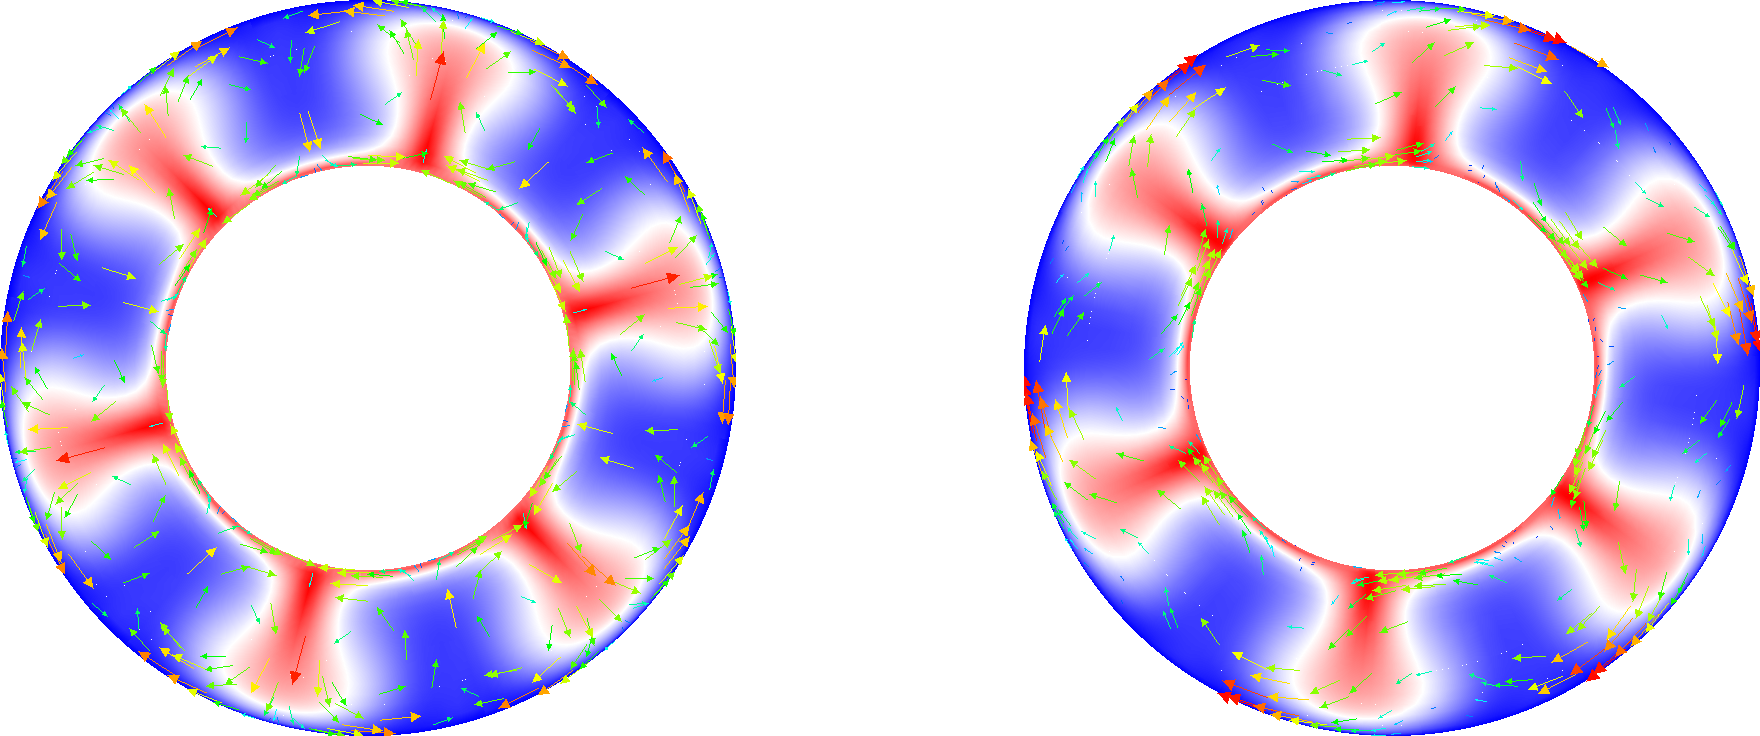
\includegraphics[width=0.8\textwidth]{rigid_rotation.png}
  \caption{\it Example of nullspace removal.
On the left the nullspace (a rigid rotation) is removed, and the velocity vectors accurately
show the mantle flow. On the right there is a significant clockwise rotation to the velocity
solution which is making the more interesting flow features difficult to see. }
  \label{fig:rigid_rotation}
\end{figure}


\subsection{Particles}
\label{sec:particles}

\aspect{} can, optionally, also deal with particles (sometimes called
``tracers''). Particles can be thought of as point-like objects that are simply
advected along with the flow. In other words, if $\mathbf u(\mathbf x,t)$ is the
flow field that results from solving equations
\eqref{eq:stokes-1}--\eqref{eq:stokes-2}, then the $k$th particle's position
satisfies the equations
\begin{align}
  \frac{\partial}{\partial t} \mathbf x_k(t)
  = \mathbf u(\mathbf x_k(t),t).
\end{align}
The initial positions of all particles also need to be given and are usually
either chosen randomly, based on a fixed pattern, or are read from a file.

Particles are typically used to track visually where material that starts
somewhere ends up after some time of a simulation. It can also be used to track
the \textit{history} of the volume of the fluid that surrounds a particle, for
example by tracking how much strain has accumulated, or what the minimal or maximal
temperature may have been in the medium along the trajectory of a particle. To
this end, particles can carry \textit{properties}. These are scalar-
or vector-valued quantities that are attached to each particle, that are
initialized at the beginning of a simulation, and that are then updated at each time step. In other words, if we
denote by $\mathbf p_{k,m}(t)$ the value of the $m$th property attached to
the $k$th particle, then $\mathbf p_{k,m}(t)$ will satisfy a differential
equation of the form
\begin{align*}
  \frac{\partial}{\partial t} \mathbf p_{k,m}(t)
  = \mathbf g_m\left(\mathbf p_{k,m},
  p(\mathbf x_k(t),t)), T(\mathbf x_k(t),t)),
  \varepsilon(\mathbf u(\mathbf x_k(t),t)),
  \mathfrak c(\mathbf x_k(t),t)\right).
\end{align*}
The exact form of $\mathbf g_m$ of course depends on what exactly a particular
property represents. Like with compositional fields (see
Section~\ref{sec:compositional}), it is possible to describe the right hand side
$\mathbf g_m$ in ways that also allows for impulse (delta) functions in time.

How particles are used in practice is probably best explained using examples. To
this end, see in particular Section~\ref{sec:cookbooks-particles}. All
particle-related input parameters are listed in
Section~\ref{parameters:Postprocess/Particles}. The implementation of particles is
discussed in great detail in \cite{gassmoeller_particles}.



\subsection{Geometric Multigrid}
\label{sec:gmg}

\aspect{} can optionally use a Geometric Multigrid Solver (GMG) for the efficient solution
of the Stokes system (velocity and pressure). When used correctly, this can
reduce the compute time spent in the solver by about a factor of 3,
and decrease the memory requirements by a factor of 10.
For more details
about the method see~\cite{clevenger_stokes19,clevenger_par_gmg}.

To take advantage of the GMG solver, you need to:
\begin{enumerate}
 \item Enable it in your parameter file, namely:
\lstinputlisting[language=prmfile]{cookbooks/overview/doc/gmg-enable.part.prm.out}
  See~\ref{parameters:Solver_20parameters/Stokes_20solver_20parameters} for other
  parameters that influence the solver behavior.

\item
  \index[prmindex]{Material averaging}
  \index[prmindexfull]{Material model!Material averaging}
  The GMG solver requires that the viscosity is averaged, either as a constant (for example by using harmonic averaging)
  or as a $Q_1$ averaging. (See Section~\ref{sec:sinker-with-averaging}
  for more about averaging.) Averaging other properties is optional. You can
  use
\lstinputlisting[language=prmfile]{cookbooks/overview/doc/gmg-average.part.prm.out}
for example. Note that $Q_1$ averaging is a bit slower than averaging to a constant per cell, but it
might provide more accurate solutions.

\item Run in release mode. The GMG solver depends on running optimized code, so using optimized mode
is more important than for other parts of ASPECT to get good
performance. (Of course, the GMG solver also runs in debug mode, and
you should do so while setting up a model. You will just not get the
same speedup from the non-GMG to the GMG solver in debug mode as you
get in release mode.)

\item Enable vectorization optimizations. The GMG solver takes advantage of special instructions (AVX2, AVX512)
in modern CPUs and requires these do be enabled when compiling \dealii{}. This can be achieved by passing the
compiler flag \texttt{CMAKE\_CXX\_FLAGS='-march=native'} to CMake or setting \texttt{NATIVE\_OPTIMIZATIONS=true} in \texttt{candi.cfg} when using candi (see~\ref{sec:installation} for more information).
When you have vectorization enabled, ASPECT will report something like
this:
\begin{lstlisting}[frame=single,language=ksh]
-----------------------------------------------------------------------------
-- This is ASPECT, the Advanced Solver for Problems in Earth's ConvecTion.
--     . version 2.3.0-pre
--     . using deal.II 9.2.0
--     .       with 64 bit indices and vectorization level 3 (512 bits)
--     . using Trilinos 12.10.1
--     . using p4est 2.2.0
--     . running in OPTIMIZED mode
--     . running with 114688 MPI processes
-----------------------------------------------------------------------------

Vectorization over 8 doubles = 512 bits (AVX512), VECTORIZATION_LEVEL=3
\end{lstlisting}
Without optimizations enabled, the output will be ``and vectorization
level 1 (128 bits)'' in the fourth line above.
\end{enumerate}




\section{Installation}
\label{sec:installation}

There are three distinct ways to install ASPECT -- compilation
from source, installing a virtual machine, and using a Docker container --
each providing distinct advantages and disadvantages. In this section we
describe all three options and start with a summary of their properties to
guide users to an informed decision about the best option for their purpose.

\begin{table}[htb]
  \center
  \begin{tabular}{|c|ccc|}
    \hline
    Feature & Compile \& Install & Virtual Machine & Docker Container \\
    \hline
    Speed overhead          & 0\%   & 30\%     & 0--5\%    \\
    Disk overhead           & 0~GB  & 1~GB     & 200~MB       \\
    Knowledge required      & Much  & Very Little & Little    \\
    Root privileges required & No   & No (installed VM software) & Partially  \\
    Embedded in native environment & Yes & No  & Partially    \\
    MacOS support           & Yes   & Yes      & Yes    \\
    Windows support         & No    & Yes      & Yes    \\
    Local parallelization   & Yes   & Yes      & Yes            \\
    Massively parallel computations & Yes & No & No \\
    Modifying ASPECT        & Possible & Possible & Possible \\
    Configuring dependencies & Possible & No   & No \\ \hline
  \end{tabular}
  \caption{\it Features of the different installation options of \aspect{}.}
  \label{tab:install-options}
\end{table}

The available options can be best presented in form of typical use cases:

\begin{enumerate}
\item Virtual Machine (\aspect{} beginner and tutorial participant): The
virtual machine image provides a fully prepared user environment that contains
installations of \aspect{}, all required libraries, and visualization software
on top of a full Linux environment. This way beginning users and tutorial
participants can work in a unified  environment, thus minimizing installation
time and technical problems. Due to the overhead of virtualizing a full
operating system this installation typically needs more space, and is
approximately 30~\% slower than a native installation. Additionally working in a
virtual machine `feels' differently from working in your usual desktop
environment. The virtual machine can be run on all host operating systems that
can run a virtualization software like VirtualBox (e.g. Linux, Apple MacOS,
Microsoft Windows).

\item Docker Container (advanced user with no need to configure/change the
underlying libraries, possibly changing parts of \aspect): Docker containers are
lightweight packages that only encapsulate the minimal dependencies to run an
application like \aspect{} on top of the host operating system. They allow easy
installation and usage of \aspect{} in a unified environment, while relying on
the user's operating system to provide visualization software and model input
data. When compared to the virtual machine it is simple to exchange files
between the host operating system and the docker container, and it provides the
benefit to work in the desktop environment you are used to. They have very
little overhead in terms of memory and speed compared to virtual machines, and
allow for reproducible computations. The container is set up with a standard
\aspect{} installation, but this can be modified by advanced users (source code
development within the container is possible).

\item Compile \& Install (advanced users and developers with the need to
reconfigure underlying libraries or running massively parallel models): The most
advanced option is to compile and install \aspect{} from source. This allows
maximal control over the underlying libraries like \trilinos{} and \dealii{}, as
well as easy modifications to \aspect{} by recompiling a modified source
directory. Our installation instructions cover most Linux and MacOS operating
systems, but incompatibilities on individual systems can always occur and make
the installation more cumbersome. If you are planning to run massively parallel
computations on a compute cluster this is likely your only option. Since
clusters usually have a very individual setup, it is always a good idea to ask
IT support staff for help when installing \aspect{}, to avoid hard to reproduce
setup problems, and performance penalties.
\end{enumerate}

\subsection{Docker Container}
\label{subsec:docker_container}

\subsubsection{Installing Docker and downloading the \aspect{} image}

Docker is a lightweight virtualization software that allows to ship
applications with all their dependencies in a simple way. It is outside of the
scope of this manual to explain all possible applications of Docker, and we
refer to the introduction (\url{https://www.docker.com/what-docker}) and
installation and quickstart guides
(\url{https://www.docker.com/products/docker}) on the Docker website for more
detailed descriptions of how to set up and use the docker engine. More
importantly Docker provides a marketplace for exchanging prepared docker images
(called Docker Hub). After setting up the docker engine downloading a
precompiled \aspect{} image from Docker Hub is as simple as typing in a
terminal:

\begin{lstlisting}[frame=single,language=ksh]
docker pull geodynamics/aspect
\end{lstlisting}

Note that the transfer size of the compressed image containing \aspect{} and
all its dependencies is about 900~MB. When extracted the image requires about
3.2~GB of disk space.

\subsubsection{Running \aspect{} models}
Although it is possible to use the downloaded \aspect{} docker image in a
number of different ways, we recommend the following workflow:

\begin{enumerate}
\item Create your \aspect{} input file in a folder of your choice (possibly
also containing any input data that is required by your model) and navigate in a
terminal into that directory.
\item Run the docker image and mount the current directory as a read-only
volume into the docker container\footnote{Note that it is possible to mount a
directory as writeable into the container. However, this is often associated
with file permission conflicts between the host system and the container.
Therefore, we recommend this slightly more cumbersome, but also more reliable
workflow.}. This is accomplished by specifying the -v flag followed by
the absolute path on the host machine, colon, absolute path within the docker
container, colon, and specifying read-only permissions as in the example below.

Make sure your parameter file specifies a model output directory \textit{other}
than the input directory, e.g. \texttt{/home/dealii/aspect/model\_output}. When
you have started the container run the aspect model inside the container. Note
that there are two \aspect{} executables in the work directory of the container:
\texttt{aspect} and \texttt{aspect-release}. For a discussion of the
different versions see Section~\ref{sec:debug-mode}, in essence: You should run
\texttt{aspect} first to check your model for errors, then run
\texttt{aspect-release} for a faster model run.

To sum up, the steps you will want to execute are:
\begin{lstlisting}[frame=single,language=ksh,showstringspaces=false]
docker run -it -v "$(pwd):/home/dealii/aspect/model_input:ro" \
  geodynamics/aspect:latest bash
\end{lstlisting}

Within the container, simply run your model by executing:

\begin{lstlisting}[frame=single,language=ksh]
./aspect model_input/your_input_file.prm
\end{lstlisting}

\item After the model has finished (or during the model run if you want to check
intermediate results) copy the model output out of the container into your
current directory. For this you need to find the name or ID of the docker
container by running \texttt{docker ps -a} in a separate terminal first. Look
for the most recently started container to identify your current \aspect{}
container.

Commands that copy the model output to the current directory could be:
\begin{lstlisting}[frame=single,language=ksh]
docker ps -a # Find the name of the running / recently closed container in the output
docker cp CONTAINER_NAME:/home/dealii/aspect/model_output .
\end{lstlisting}

\item The output data is saved inside your container even after the computation
finishes and even when you stop the container. After you have copied the data
out of the container you should therefore delete the container to avoid
duplication of output data. Even after deleting you will always be able to start
a new container from the downloaded image following step 2. Deleting the
finished container can be achieved by the \texttt{docker container prune}
command that removes any container that is not longer running.
\note{If you own other finished containers that you want to keep use
\texttt{docker container rm CONTAINER\_NAME} to only remove the container named
\texttt{CONTAINER\_NAME}.}

To remove all finished containers use the following command:
\begin{lstlisting}[frame=single,language=ksh]
docker container prune
\end{lstlisting}
Alternatively only remove a particular container:
\begin{lstlisting}[frame=single,language=ksh]
docker container rm CONTAINER_NAME
\end{lstlisting}
\end{enumerate}

You are all set. Repeat steps 1-4 of this process as necessary when updating
your model parameters.

\subsubsection{Developing \aspect{} within a container}

The above given workflow does not include advice on how to modify \aspect{}
inside the container. We recommend a slightly different workflow for advanced
users that want to modify parts of \aspect{}. The \aspect{} docker container
itself is build on top of a \dealii{} container that contains all dependencies
for compiling \aspect{}. Therefore it is possible to run the deal.II container,
mount an \aspect{} source directory from your host system and compile it inside
of the container. An example workflow could look as following (assuming you
navigated in a terminal into the modified \aspect{} source folder):

\begin{lstlisting}[frame=single,language=ksh,showstringspaces=false]
docker pull tjhei/dealii:v9.2.0-full-v9.2.0-r2-gcc5
docker run -it -v "$(pwd):/home/dealii/aspect:ro" \
  tjhei/dealii:v9.2.0-full-v9.2.0-r2-gcc5 bash
\end{lstlisting}

Inside of the container you now find a read-only \aspect{} directory that
contains your modified source code. You can compile and run a model inside the
container, e.g. in the following way:

\begin{lstlisting}[frame=single,language=ksh]
mkdir aspect-build
cd aspect-build
cmake -DCMAKE_BUILD_TYPE=Debug -DDEAL_II_DIR=$HOME/deal.II-install $HOME/aspect
./aspect $HOME/aspect/cookbooks/shell_simple_2d.prm
\end{lstlisting}

To avoid repeated recompilations of the \aspect{} source folder we recommend to
reuse the so prepared container instead of starting new containers based on the
\dealii{} image. This can be achieved by the following commands outside of the
container:

\begin{lstlisting}[frame=single,language=ksh]
docker ps -a # Find the name of the running / recently closed container in the output
docker restart CONTAINER_NAME
docker attach CONTAINER_NAME
\end{lstlisting}

For more information on the differences between using images and containers,
and how to attach additional terminals to a running container, we refer to the
docker documentation (e.g.
\url{https://docs.docker.com/engine/getstarted/step_two/}).

\subsection{Virtual Machine}

\subsubsection{Installing VM software and setting up the virtual machine}

The \aspect{} project provides an experimental virtual machine containing a
fully configured version of \aspect{}. To use this machine, you will need to
install VirtualBox (\url{http://www.virtualbox.org/}) on your machine, and then
import a virtual machine image that can be downloaded from
\url{http://www.math.clemson.edu/~heister/dealvm/}. Note, however, that the
machine image is several gigabytes in size and downloading will take a while.
After downloading and installing the virtual image it is convenient to set up a
shared folder between your host system and the virtual machine to exchange model
files and outputs.

\subsubsection{Running \aspect{} models}

The internal setup of the virtual machine is similar to the Docker container
discussed above, except that it contains a full-featured desktop environment.
Also note that the user name is \texttt{ubuntu}, not \texttt{dealii} as in the
Docker container. Again there are multiple ways to use the virtual machine, but
we recommend the following workflow:

\begin{enumerate}
\item Create your \aspect{} input file in the shared folder and start the
virtual machine.
\item Navigate in a terminal to your model directory.
\item Run your model using the provided \aspect{} executable:

\begin{lstlisting}[frame=single,language=ksh]
~/aspect/aspect your_input_file.prm
\end{lstlisting}

\item The model output should automatically appear on your host machine in the
shared directory.

\item After you have verified that your model setup is correct, you might want
to consider recompiling \aspect{} in release mode to increase the speed of the
computation. See Section~\ref{sec:debug-mode} for a discussion of debug and
release mode.

\item Visualize your model output either inside of the virtual machine
(ParaView and VisIt are pre-installed), or outside on your host system.
\end{enumerate}

You are all set. Repeat steps 1-6 of this process as necessary when updating
your model parameters.

\subsection{Local installation}

This is a brief explanation of how to compile and install the required dependencies and
\aspect{} itself. This installation procedure guarantees fastest runtimes, and largest flexibility,
but usually requires more work than the options mentioned in the previous sections.
While it is possible to install ASPECT's dependencies in particular \pfrst{}, \trilinos{},
and \dealii{} manually, we recommend to use the
\texttt{candi} software (see \url{https://github.com/dealii/candi}). \texttt{candi} was written
as an installation program for deal.II, and includes a number of system specific instructions
that will be listed when starting the program. It can be flexibly configured to allow for
non-default compilers or libraries (e.g. Intel's MKL instead of LAPACK) by changing entries
in the configuration file \texttt{candi.cfg}, or by providing platform specific installation files.

In case you encounter problems during the installation, please consult our wiki
(\url{https://github.com/geodynamics/aspect/wiki}) for frequently asked
questions and special instructions for MacOS users, before posting your
questions on the forum (\url{https://community.geodynamics.org/c/aspect}).

\subsubsection{System prerequisites}

\texttt{candi} will show system specific instructions on startup, but its prerequisites
are relatively widely used and packaged
for most operating systems. You will need compilers for C, C++ and
Fortran, the GNU make system, the CMake build system, and the libraries and
header files of BLAS, LAPACK and zlib, which is used for compressing
the output data. To use more than one process for your computations
you will need to install a MPI library, its headers and the
necessary executables to run MPI programs. There are some optional packages
for additional features, like the HDF5 libraries for additional output formats
 and Numdiff for checking \aspect{}'s test
results with reasonable accuracy, but these are not strictly required, and in
some operating systems they are not available as packages but need to be
compiled from scratch.
Finally, for obtaining a recent development version of \aspect{} you will
need the git version control system.

An exemplary command to obtain all required packages on Ubuntu 14.04 would be:
\begin{verbatim}
sudo apt-get install build-essential \
                     cmake \
                     gcc \
                     g++ \
                     gfortran \
                     git \
                     libblas-dev \
                     liblapack-dev \
                     libopenmpi-dev \
                     numdiff \
                     openmpi-bin \
                     zlib1g-dev
\end{verbatim}

\subsubsection{Using candi to compile dependencies}

In its default configuration \texttt{candi} downloads and
compiles a \dealii{} configuration that is able to run \aspect, but it
also contains a number of packages that are not required (and that can
be safely disabled if problems occur during the
installation). We require at least the packages \pfrst{}, \trilinos{},
and finally \dealii{}.

At the time of this writing \texttt{candi} will install \pfrst{} 2.2,
\trilinos{} 12.18.1, and \dealii{} 9.3.0.
We strive to keep the development version of \aspect{} compatible with
the latest release of \dealii{} and the current \dealii{} development
version at any time, and we usually support several older versions of
\pfrst{} and \trilinos{}.

\begin{enumerate}
\item \textit{Obtaining candi:} Download \texttt{candi} by running
    \begin{verbatim}
    git clone https://github.com/dealii/candi
    \end{verbatim}
    in a directory of your choice.

\item \textit{Installing \dealii{} and its dependencies:} Execute \texttt {candi} by running
    \begin{verbatim}
    cd candi
    ./candi.sh -p INSTALL_PATH
    \end{verbatim}
    (here we assume you replace \texttt{INSTALL\_PATH} by the path were
    you want to install all dependencies and \dealii{}, typically a directory inside
    \texttt{\$HOME/bin} or a similar place).
    This step might take a long time, but can be parallelized by adding
    \texttt{-jN}, where
    \texttt{N} is the number of CPU cores available on your computer. Further configuration options
    and parameters are listed at \url{https://github.com/dealii/candi}. In case you encounter
    problems during this step, please read the error message, and consult our wiki
    (\url{https://github.com/geodynamics/aspect/wiki}) for common installation problems,
    before asking on the forum (\url{https://community.geodynamics.org/c/aspect}).

\item You may now want to configure your environment to make it aware of the newly installed
    packages. This can be achieved by adding the line
    \texttt{source INSTALL\_PATH/configuration/enable.sh} to the file responsible for setting
    up your shell environment\footnote{For bash this would be the file \texttt{\~{}/.bashrc}.}
    (again we assume you replace \texttt{INSTALL\_PATH} by the patch chosen in the previous step).
    Then close the terminal and open it again to activate the change.

\item \textit{Testing your installation:} Test that your installation works
  by compiling the {\texttt{step-32}} example that you can find in
  {\texttt{\$DEAL\_II\_DIR/examples/step-32}}. Prepare and compile by running {\texttt{cmake . \&\& make}}
  and run with {\texttt{mpirun -n 2 ./step-32}}.

\end{enumerate}

Congratulations, you are now set up for compiling \aspect{} itself.

\subsubsection{Obtaining \aspect{} and initial configuration}

The development version of \aspect{} can be downloaded by executing the command
\begin{verbatim}
 git clone https://github.com/geodynamics/aspect.git
\end{verbatim}
If {\texttt{\$DEAL\_II\_DIR}} points to your \dealii{} installation, you can configure
\aspect{} by running
\begin{verbatim}
 mkdir build; cd build; cmake ..
\end{verbatim}
in the \aspect{} directory created by the {\texttt{git clone}} command above.
If you did not set {\texttt{\$DEAL\_II\_DIR}} you have to supply cmake with the location:
\begin{verbatim}
 cmake -DDEAL_II_DIR=/u/username/deal-installed/ ..
\end{verbatim}

This will create an ``out-of-source`` build, where the build directory is
different from the source directory. While in-source builds (where you run
\texttt{cmake .} in your source directory), are supported, we strongly
recommend an out-of-source build as described above. Specifically, running
the whole test suite (see Section~\ref{sec:running_tests}) is only supported
this way.

\subsubsection{Compiling \aspect{} and generating documentation}
\label{sec:compiling}

After downloading \aspect{} and having built the libraries it builds on, you
can compile it by typing
\begin{verbatim}
  make
\end{verbatim}
on the command line (or \texttt{make -jN} if you have multiple processors in
your machine, where \texttt{N} is the number of processors). This builds the
\aspect{} executable which will reside in the \texttt{build} directory
and will be named \texttt{aspect}. To run \aspect{} from the main source directory
you would need to reference it as \texttt{./build/aspect}.
If you intend to
modify \aspect{} for your own experiments, you may want to also generate
documentation about the source code. This can be done using the command
\begin{verbatim}
  cd doc; make
\end{verbatim}
which assumes that you have the \texttt{doxygen} documentation generation tool
installed. Most Linux distributions have packages for \texttt{doxygen}. The
result will be the file \url{doc/doxygen/index.html} that is the starting
point for exploring the documentation.


%%%%%%%%%%%%%%%%%%%%%%

\section{Running \aspect}
\label{sec:running}

\subsection{First steps}
\label{sec:first-steps}
Before trying to set up a model to answer your particular research questions,
we advise you to get familiar with \aspect{} and its functionalities by
following these steps:
\begin{enumerate}
\item Watch the CIG \aspect{} tutorials (\url{https://www.youtube.com/playlist?list=PLdy04DoEepEyeS_HZwa0Ws0kW5Rs2wsQ6})
that will show you how to run \aspect{} and construct new setups yourself.
\item Go through the cookbooks in this manual, see Section~\ref{sec:cookbooks}.
\item Go through the benchmarks in this manual, see Section~\ref{sec:cookbooks-benchmarks}.
\item If you want to use some existing functionality that is not discussed in these resources,
search in the extensive tests directory. For example, to search for an initial temperature condition called
``spherical gaussian perturbation'' while in the \aspect{} directory, type:
\begin{verbatim}
  grep 'spherical gaussian perturbation' tests/*.prm
\end{verbatim}
This command will show you all the test input files that use this initial temperature condition.
You can also look up any of the parameters used in the input files in this manual.
\item Have a look at the \aspect{} GitHub repository. Here you can see the planned developments
(\url{https://github.com/geodynamics/aspect/projects/2}), current issues that others have reported
(\url{https://github.com/geodynamics/aspect/issues}), and what is currently being worked on
(\url{https://github.com/geodynamics/aspect/pulls}).
\item Have a look at our discussion forum when your model behaves unexpectedly
or you need functionality that does not exist yet. The \aspect{} community can tell you
whether they experienced something similar or are already working on the topic.
\item If you experience unexpected behavior that you expect is a bug and this problem
has not been reported as an issue on GitHub, please create a new issue so that everybody
is aware of the potential problem and can think of a fix. When creating a new issue,
it is very useful if you can provide a minimum working example, i.e. a small test setup
that demonstrates the issue and does not require modifications to the code. You can for example
modify one of the existing test input files, which typically take less than a minute to
run using only a few cores.
The test input file and an image illustrating the problem can be attached to the issue.
\end{enumerate}

\subsection{Overview}
\label{sec:running-overview}

After compiling \aspect{} as described above, you should have an executable
file in the build directory. It can be called in the build directory as follows:
\begin{verbatim}
  ./aspect parameter-file.prm
\end{verbatim}
or, if you want to run the program in parallel, using something like
\begin{verbatim}
  mpirun -np 4 ./aspect parameter-file.prm
\end{verbatim}
to run with 4 processors. In either case, the argument denotes the (path and)
name of a file that contains input parameters.%
\footnote{As a special case, if you call \aspect{} with an argument that
consists of two dashes, ``\texttt{-{}-}'', then the arguments will be read from
the standard input stream of the program. In other words, you could type the
input parameters into your shell window in this case (though that would be
cumbersome, \aspect{} would seem to hang until you finish typing all of your
input into the window and then terminating the input stream by typing
\texttt{Ctrl-D}). A more common case would be to use Unix pipes so that the
default
input of \aspect{} is the output of another program, as in a command like
\texttt{cat parameter-file.prm.in | mypreprocessor | ./aspect -{}-}, where
\texttt{mypreprocessor} would be a program of your choice that somehow
transforms the file \texttt{parameter-file.prm.in} into a valid input file,
for example to systematically vary one of the input parameters.

If you want to run \aspect{} in parallel, you can do something like
\texttt{cat parameter-file.prm.in | mypreprocessor | mpirun -np 4 ./aspect
  -{}-}. In cases like this, \texttt{mpirun} only forwards the output of
\texttt{mypreprocessor} to the first of the four MPI processes, which then
sends the text to all other processors.}
When you download \aspect{}, there are a number of sample input files in the
\texttt{cookbooks} directory, corresponding to the examples discussed in
Section~\ref{sec:cookbooks}, and input files for some of the benchmarks discussed
in Section~\ref{sec:cookbooks-benchmarks} are located in the \texttt{benchmarks}
directory. A full description of all parameters one can specify in these files
is given in Section~\ref{sec:parameters}.

Running \aspect{} with an input file
\footnote{For example by running \texttt{./aspect ../cookbooks/convection-box/convection-box.prm} in
your build directory.}
will produce output that will look
something like this (numbers will all be different, of course):
\begin{lstlisting}[frame=single,language=ksh]
-----------------------------------------------------------------------------
-- This is ASPECT, the Advanced Solver for Problems in Earth's ConvecTion.
--     . version 2.0.0-pre (include_dealii_version, c20eba0)
--     . using deal.II 9.0.0-pre (master, 952baa0)
--     . using Trilinos 12.10.1
--     . using p4est 2.0.0
--     . running in DEBUG mode
--     . running with 1 MPI process
-----------------------------------------------------------------------------

Number of active cells: 1,536 (on 5 levels)
Number of degrees of freedom: 20,756 (12,738+1,649+6,369)

*** Timestep 0:  t=0 years

   Rebuilding Stokes preconditioner...
   Solving Stokes system... 30+3 iterations.
   Solving temperature system... 8 iterations.

Number of active cells: 2,379 (on 6 levels)
Number of degrees of freedom: 33,859 (20,786+2,680+10,393)

*** Timestep 0:  t=0 years

   Rebuilding Stokes preconditioner...
   Solving Stokes system... 30+4 iterations.
   Solving temperature system... 8 iterations.

   Postprocessing:
     Writing graphical output: output/solution/solution-00000
     RMS, max velocity:        0.0946 cm/year, 0.183 cm/year
     Temperature min/avg/max:  300 K, 3007 K, 6300 K
     Inner/outer heat fluxes:  1.076e+05 W, 1.967e+05 W

*** Timestep 1:  t=1.99135e+07 years

   Solving Stokes system... 30+3 iterations.
   Solving temperature system... 8 iterations.

   Postprocessing:
     Writing graphical output: output/solution/solution-00001
     RMS, max velocity:        0.104 cm/year, 0.217 cm/year
     Temperature min/avg/max:  300 K, 3008 K, 6300 K
     Inner/outer heat fluxes:  1.079e+05 W, 1.988e+05 W

*** Timestep 2:  t=3.98271e+07 years

   Solving Stokes system... 30+3 iterations.
   Solving temperature system... 8 iterations.

   Postprocessing:
     RMS, max velocity:       0.111 cm/year, 0.231 cm/year
     Temperature min/avg/max: 300 K, 3008 K, 6300 K
     Inner/outer heat fluxes: 1.083e+05 W, 2.01e+05 W

*** Timestep 3:  t=5.97406e+07 years

...
\end{lstlisting}

The output starts with a header that lists the used \aspect{}, \dealii{},
\trilinos{} and \pfrst{} versions as well as the mode you compiled \aspect{} in
(see \ref{sec:debug-mode}), and the number of parallel processes
used\footnote{If you used the \texttt{git} version control system to download
\aspect{} and/or \dealii{}, as in this example, you will also get the current
branch, and unique revision identifier for the current version. This is very
important if you modify either software between releases, or you use a
development version that is not an official release. Note that this revision
can not track changes you made to the software that are not part of a git
commit.}.  With this information we strive to make
\aspect{} models as reproducible as possible.

The following output depends on the model, and in this case was produced by
a parameter file that, among other settings, contained the following values
(we will discuss many such input files in Section~\ref{sec:cookbooks}:
\lstinputlisting[language=prmfile]{cookbooks/overview/doc/simple.prm.out}

In other words, these run-time parameters specify that we should start with a
geometry that represents a spherical shell (see
Sections~\ref{parameters:Geometry_20model} and
\ref{parameters:Geometry_20model/Spherical_20shell} for details). The coarsest
mesh is refined 4 times globally, i.e., every cell is refined into four
children (or eight, in 3d) 4 times. This yields the initial number of 1,536
cells on a mesh hierarchy that is 5 levels deep. We then solve the problem
there once and, based on the number of adaptive refinement steps at the
initial time set in the parameter file, use the solution so computed to refine
the mesh once adaptively (yielding 2,379 cells on 6 levels) on which we start
the computation over at time $t=0$.

Within each time step, the output indicates the number of iterations performed
by the linear solvers, and we generate a number of lines of output by the
postprocessors that were selected (see
\index[prmindex]{List of postprocessors}
\index[prmindexfull]{Postprocess!List of postprocessors}
Section~\ref{parameters:Postprocess}). Here, we have selected to run all
postprocessors that are currently implemented in \aspect{} which includes the
ones that evaluate properties of the velocity, temperature, and heat flux as
well as a postprocessor that generates graphical output for visualization.

While the screen output is useful to monitor the progress of a simulation,
its lack of a structured output makes it not useful for later plotting things
like the evolution of heat flux through the core-mantle boundary. To this end,
\aspect{} creates additional files in the output directory selected in the
input parameter file
\index[prmindex]{Output directory}
\index[prmindexfull]{Output directory}
(here, the \texttt{output/} directory relative to the
directory in which \aspect{} runs). In a simple case, this will look as
follows:
\begin{lstlisting}[frame=single,language=ksh]
aspect> ls -l output/
total 932
-rw-rw-r-- 1 bangerth bangerth  11134 Dec 11 10:08 depth_average.gnuplot
-rw-rw-r-- 1 bangerth bangerth  11294 Dec 11 10:08 log.txt
-rw-rw-r-- 1 bangerth bangerth     42 Dec 11 10:07 original.prm
-rw-rw-r-- 1 bangerth bangerth 326074 Dec 11 10:07 parameters.prm
-rw-rw-r-- 1 bangerth bangerth 577138 Dec 11 10:07 parameters.tex
drwxr-xr-x 2 bangerth bangerth   4096 Dec 11 10:08 solution
-rw-rw-r-- 1 bangerth bangerth    484 Dec 11 10:08 solution.pvd
-rw-rw-r-- 1 bangerth bangerth    451 Dec 11 10:08 solution.visit
-rw-rw-r-- 1 bangerth bangerth   8267 Dec 11 10:08 statistics
\end{lstlisting}
The purpose of these files is as follows:
\begin{itemize}

\item \textit{Screen output:} The file \texttt{output/log.txt} contains a copy
  of the output that is printed to the terminal when you run \aspect{}.

\item \textit{A listing of all run-time parameters:} The file
  \texttt{output/original.prm} is a copy of the parameter file that was used
  in this computation. It is often useful to save this file together with
  simulation data to allow for the easy reproduction of computations later on.

  The \texttt{output/parameters.prm} file contains a complete listing of all
  run-time parameters. In particular, this includes the ones that have been
  specified in the input parameter file passed on the command line, but it
  also includes those parameters for which defaults have been used. This file
  can also be used to explore all available parameters and possible options as
  it contains the documentation of all parameters.

  Finally, there is \texttt{output/parameters.tex}, that lists the parameters
  like \texttt{output/parameters.prm} in \LaTeX{} format, and
  \texttt{output/parameters.json} in JSON format.

  While \texttt{output/parameters.prm} contains all parameters (with their
  default values if they were not specified), all formatting and comments are
  lost. As \texttt{output/original.prm} is identical to the prm you started
  \aspect{} with, it preserves comments and formatting while not outputting
  the default values (or documentation).

\item \textit{Graphical output files:} One of the postprocessors chosen
  in the parameter file used for this computation is the one that generates
  output files that represent the solution at certain time steps. The screen output
  indicates that it has run at time step 0, producing output files that start
  with \texttt{output/solution/solution-00000}. Depending on the settings in the
  parameter file, output will be generated every so many seconds or years of
  simulation time, and subsequent output files will then start with
  \texttt{output/solution/solution-00001}, all placed in the
  \texttt{output/solution} subdirectory. This is because there are often
  \textit{a lot} of output files: For many time steps, times the number of
  processors, so they are placed in a subdirectory so as not to make it more
  difficult than necessary to find the other files.

  At the current time, the
  default is that \aspect{} generates this output in VTK format%
  \footnote{The output is in fact in the VTU version of the VTK file
    format. This is the XML-based version of this file format in which
    contents are compressed. Given that typical file sizes for 3d simulation
    are substantial, the compression saves a significant amount of disk
    space.}  as that is widely used by a number of excellent visualization
  packages and also supports parallel visualization.%
  \footnote{The underlying \dealii{} package actually supports output in
    around a dozen different formats, but most of them are not very useful for
    large-scale, 3d, parallel simulations. If you need a different format than
    VTK, you can select this using the run-time parameters discussed in
    Section~\ref{parameters:Postprocess/Visualization}.}  If
  the program has been run with multiple MPI processes, then the list of
  output files will be \texttt{output/solution/solution-XXXXX.YYYY}
  denoting that this the \texttt{XXXXX}th time we create output files and that
  the file was generated by the \texttt{YYYY}th processor.

  VTK files can be visualized by many of the large visualization packages. In
  particular, the
  \href{https://visit.llnl.gov}{Visit} and
  \href{http://www.paraview.org/}{ParaView} programs, both
  widely used, can read the files so created. However, while VTK has become a
  de-facto standard for data visualization in scientific computing, there
  doesn't appear to be an agreed upon way to describe which files jointly make
  up for the simulation data of a single time step (i.e., all files with the
  same \texttt{XXXXX} but different \texttt{YYYY} in the example above). Visit
  and ParaView both have their method of doing things, through \texttt{.pvtu} and
  \texttt{.visit} files. To make it easy for you to view data, \aspect{}
  simply creates both kinds of files in each time step in which graphical data
  is produced, and these are then also placed into the subdirectories as
  \texttt{output/solution/solution-XXXXX.pvtu} and
  \texttt{output/solution/solution-XXXXX.visit}.

  The final two files of this kind, \texttt{output/solution.pvd} and
  \texttt{output/solution.visit}, are files that
  describes to ParaView and Visit, respectively, which
  \texttt{output/solution/solution-XXXXX.pvtu} and
  \texttt{output/solution/solution-XXXXX.YYYY.vtu} jointly form a complete
  simulation.
  In the former case, the file lists the \texttt{.pvtu} files of all
  timesteps together with the simulation time to which they correspond. In the
  latter case, it actually lists all \texttt{.vtu} that belong to one
  simulation, grouped by the timestep they correspond to.
  To visualize an entire simulation, not just a single time step, it is
  therefore simplest to just load one of these files, depending on whether you
  use ParaView or Visit.%
  \footnote{At the time of writing this, current versions of Visit (starting
    with version 2.5.1) actually have a bug that prevents them from
    successfully reading the \texttt{output/solution.visit} or
    \texttt{output/solution/solution-XXXXX.visit} files -- Visit believes that
    each of these files corresponds to an individual time step, rather than that a whole
    group of files together form one time step. This bug is not fixed in Visit
    2.6.3, but may be fixed in later versions.}
  Because loading an \textit{entire} simulation is the most common use case,
  these are the two files you will most often load, and so they are placed in
  the \texttt{output} directory, not the subdirectory where the actual
  \texttt{.vtu} data files are located.

  For more on visualization, see also Section~\ref{sec:viz}.

\item \textit{A statistics file:} The \texttt{output/statistics} file contains
  statistics collected during each time step, both from within the simulator
  (e.g., the current time for a time step, the time step length, etc.) as well
  as from the postprocessors that run at the end of each time step. The file
  is essentially a table that allows for the simple production of time
  trends. In the example above, and at the time when we are writing this
  section, it looks like this:
  \begin{lstlisting}[frame=single,language=ksh,showstringspaces=false]
# 1: Time step number
# 2: Time (years)
# 3: Iterations for Stokes solver
# 4: Time step size (year)
# 5: Iterations for temperature solver
# 6: Visualization file name
# 7: RMS velocity (m/year)
# 8: Max. velocity (m/year)
# 9: Minimal temperature (K)
# 10: Average temperature (K)
# 11: Maximal temperature (K)
# 12: Average nondimensional temperature (K)
# 13: Core-mantle heat flux (W)
# 14: Surface heat flux (W)
0 0.000e+00 33 2.9543e+07 8                             "" 0.0000 0.0000 0.0000 0.0000    ...
0 0.000e+00 34 1.9914e+07 8 output/solution/solution-00000 0.0946 0.1829 300.00 3007.2519 ...
1 1.991e+07 33 1.9914e+07 8 output/solution/solution-00001 0.1040 0.2172 300.00 3007.8406 ...
2 3.982e+07 33 1.9914e+07 8                             "" 0.1114 0.2306 300.00 3008.3939 ...
  \end{lstlisting}
  The actual columns you have in your statistics file may differ from the ones above,
  but the format of this file should be obvious. Since the hash mark is a comment
  marker in many programs (for example, \texttt{gnuplot} ignores lines in text
  files that start with a hash mark), it is simple to plot these columns as time
  series. Alternatively, the data can be imported into a spreadsheet and
  plotted there.
\note{As noted in Section~\ref{sec:non-dimensional}, \aspect{} can be
  thought of as using the meter-kilogram-second (MKS, or SI) system. Unless otherwise noted,
  the quantities in the output file are therefore also in MKS units.}

  A simple way to plot the contents of this file is shown in Section~\ref{sec:viz-stat}.

\item \textit{Output files generated by other postprocessors:} Similar to the
  \texttt{output/statistics} file, several of the existing
  postprocessors one can select from the parameter file generate their
  data in their own files in the output directory. For example, \aspect{}'s
  ``depth average'' postprocessor will write depth-average statistics into
  the file \texttt{output/depth\_average.gnuplot}.
  Input parameters chosen in the input file control how often this file is
  updated by the postprocessor, as well as what graphical file format to use (if
  anything other than \texttt{gnuplot} is desired).

  By default, the data is written in text format that can be easily visualized,
  see for example Figure~\ref{fig:depthaverage}. The plot
  shows how an initially linear temperature profile forms upper and lower
  boundary layers.

\begin{figure}[tbp]
  \centering
  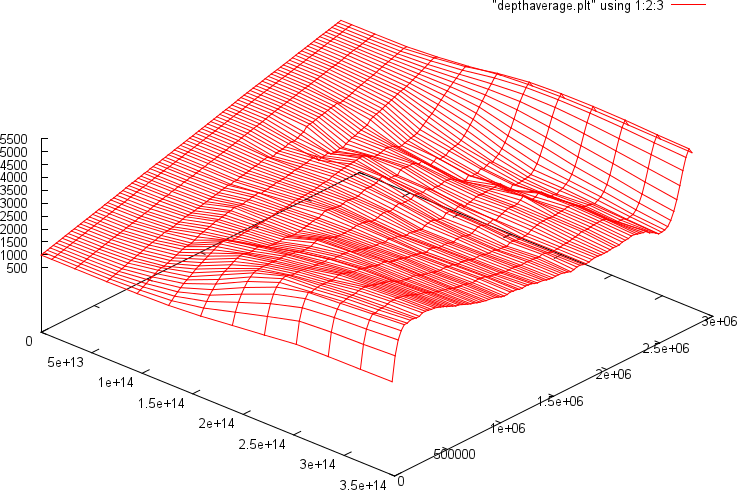
\includegraphics[width=0.6\textwidth]{depthaverage2.png}
  \caption{\it Example output for depth average statistics. On the left axis are 13 time
  steps, on the right is the depth (from the top at 0 to the bottom of the mantle on the
  far right), and the upwards pointing axis is the average temperature. This
  plot is generated by gnuplot, but the depth averages can be written in many
  other output formats as well, if preferred (see
  Section~\ref{parameters:Postprocess/Depth_20average}).}
  \label{fig:depthaverage}
\end{figure}

\end{itemize}

There are other parts of \aspect{} that may also create files in the output
directory. For example, if your simulation includes advecting along particles
(see Section~\ref{sec:particles}), then visualization information for these
particles will also appear in this file. See
Section~\ref{sec:cookbooks-particles} for an example of how this looks like.


\subsection{Selecting between 2d and 3d runs}
\label{sec:2d-vs-3d}

\aspect{} can solve both two- and three-dimensional problems.%
\footnote{For a description of what exactly we mean when we consider
two-dimensional models, see Section~\ref{sec:meaning-of-2d}.}
You select which one you want by putting a line like the following into
\index[prmindex]{Dimension}
\index[prmindexfull]{Dimension}
the parameter file (see Section~\ref{sec:parameters}):
\lstinputlisting[language=prmfile]{cookbooks/overview/doc/dim.part.prm.out}

Internally, dealing with the dimension builds on a feature in
\dealii{}, upon which \aspect{} is based, that is called
\textit{dimension-independent programming}. In essence, what this does is that
you write your code only once in a way so that the space dimension is a
variable (or, in fact, a template parameter) and you can compile the code for
either 2d or 3d. The advantage is that codes can be tested and debugged in 2d
where simulations are relatively cheap, and the same code can then be
re-compiled and executed in 3d where simulations would otherwise be
prohibitively expensive for finding bugs; it is also a useful feature when
scoping out whether certain parameter settings will have the desired effect by
testing them in 2d first, before running them in 3d. This feature is discussed
in detail in the
\href{https://www.dealii.org/developer/doxygen/deal.II/step_4.html}{\dealii{}
  tutorial program step-4}.
Like there, all the functions and classes in
\aspect{} are compiled for both 2d and 3d. Which dimension is actually
called internally depends on what you have set in the input file, but
in either case, the machine code generated for 2d and 3d results from
the same source code and should, thus, contain the same set of
features and bugs. Running in 2d and 3d should therefore yield
comparable results. Be prepared to wait much longer for
computations to finish in the latter case, however.


\subsection{Debug or optimized mode}
\label{sec:debug-mode}

\aspect{} utilizes a \dealii{} feature called \textit{debug
  mode}. By default, \aspect{} uses debug mode, i.e., it calls a version of
the \dealii{} library that contain lots of checks for the correctness of
function arguments, the consistency of the internal state of data structure,
etc. If you program with \dealii{}, for example to extend \aspect{}, it has
been our experience over the years that, by number, most programming errors are of the
kind where one forgets to initialize a vector, one accesses data that has not
been updated, one tries to write into a vector that has ghost elements,
etc. If not caught, the result of these bugs is that parts of the program use
invalid data (data written into ghost elements is not communicated to other
processors), that operations simply make no sense (adding vectors of different
length), that memory is corrupted (writing past the end of an array) or, in
rare and fortunate cases, that the program simply crashes.

Debug mode is designed to catch most of these errors: It enables some 7,300
assertions (as of late 2011) in \dealii{} where we check for errors like the
above and, if the condition is violated, abort the program with a detailed
message that shows the failed check, the location in the source code, and a
stacktrace how the program got there. The downside of debug mode is, of
course, that it makes the program much slower -- depending on application by a
factor of 4--10. An example of the speedup one can get is shown in
Section~\ref{sec:cookbooks-simple-box}.

\aspect{} by default uses debug mode because most users will want to play with
the source code, and because it is also a way to verify that the compilation
process worked correctly. If you have verified that the program runs correctly
with your input parameters, for example by letting it run for the first 10
time steps, then you can switch to optimized mode by compiling \aspect{}
with the command\footnote{Note that this procedure also changed with the switch to cmake.}
\begin{verbatim}
 make release
\end{verbatim}
and then compile using
\begin{verbatim}
 make
\end{verbatim}
To switch back to debug mode type:
\begin{verbatim}
 make debug
\end{verbatim}

\note{It goes without saying that if you make significant modifications to the
  program, you should do the first runs in debug mode to verify that your
  program still works as expected.}


\subsection{Visualizing results}
\label{sec:viz}

Among the postprocessors that can be selected in the input parameter file (see
Sections~\ref{sec:running-overview} and
\ref{parameters:Postprocess/Visualization}) are some that can produce files in
a format that can later be used to generate a graphical visualization of the
solution variables $\mathbf u, p$ and $T$ at select time steps, or of
quantities derived from these variables (for the latter, see
Section~\ref{sec:viz-postpostprocessors}).

By default, the files that are generated are in VTU format, i.e., the
XML-based, compressed format defined by the VTK library, see
\url{http://public.kitware.com/VTK/}. This file format has become a broadly
accepted pseudo-standard that many visualization program support, including
two of the visualization programs used most widely in computational science:
Visit (see \url{https://visit.llnl.gov/}) and ParaView (see
\url{http://www.paraview.org/}). The VTU format has a number of
advantages beyond being widely distributed:
\begin{itemize}
\item It allows for compression, keeping files relatively small even for
  sizable computations.
\item It is a structured XML format, allowing other programs to read it
  without too much trouble.
\item It has a degree of support for parallel computations where every
  processor would only write that part of the data to a file that this
  processor in fact owns, avoiding the need to communicate all data to a
  single processor that then generates a single file. This requires a master
  file for each time step that then contains a reference to the individual
  files that together make up the output of a single time step. Unfortunately,
  there doesn't appear to be a standard for these master records; however,
  both ParaView and Visit have defined a format that each of these programs
  understand and that requires placing a file with ending \texttt{.pvtu} or
  \texttt{.visit} into the same directory as the output files from each
  processor. Section~\ref{sec:running-overview} gives an example of what can
  be found in the output directory.
\end{itemize}

\note{You can select other formats for output than VTU, see the run-time
  parameters in Section~\ref{parameters:Postprocess/Visualization}. However,
  none of the numerous formats currently implemented in \dealii{} other than
  the VTK/VTU formats allows for splitting up data over multiple files in case
  of parallel computations, thus making subsequent visualization of the entire
  volume impossible. Furthermore, given the amount of data \aspect{} can
  produce, the compression that is part of the VTU format is an important part
  of keeping data manageable.
\index[prmindex]{Output format}
\index[prmindexfull]{Postprocess!Visualization!Output format}
}

\subsubsection{Visualization the graphical output using \textit{Visit}}
In the following, let us discuss the process of visualizing a 2d computation
using Visit. The steps necessary for other visualization programs will
obviously differ but are, in principle, similar.

To this end, let us consider a simulation of convection in a box-shaped, 2d
region (see the ``cookbooks'' section, Section~\ref{sec:cookbooks}, and in
particular Section~\ref{sec:cookbooks-simple-box} for
the input file for this particular model). We can run the program with 4 processors using
\begin{verbatim}
  mpirun -np 4 ./aspect cookbooks/convection-box/convection-box.prm
\end{verbatim}
Letting the program run for a while will result in several output files as
discussed in Section~\ref{sec:running-overview} above.

In order to visualize one time step, follow these steps:%
\footnote{The instructions and screenshots were generated with Visit
  2.1. Later versions of Visit differ slightly in the arrangement of
  components of the graphical user interface, but the workflow and general
  idea remains unchanged.}

\begin{figure}[tbp]
  \phantom{.}
  \hfill
  \subfigure[]{
    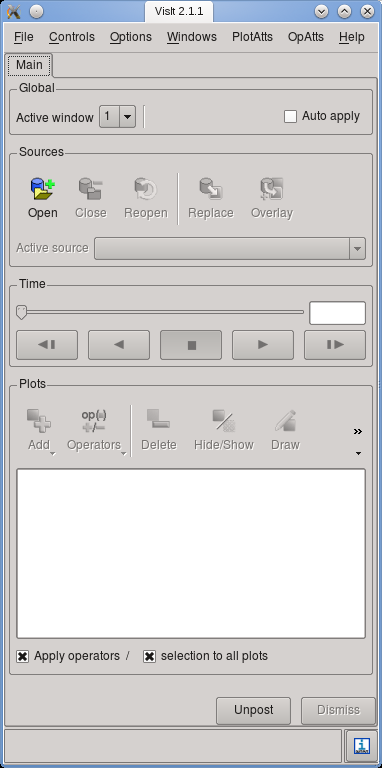
\includegraphics[width=0.24\textwidth]{viz/visit/visit-1.png}
    \label{fig:visit-1:a}
  }
  \hfill
  \subfigure[]{
    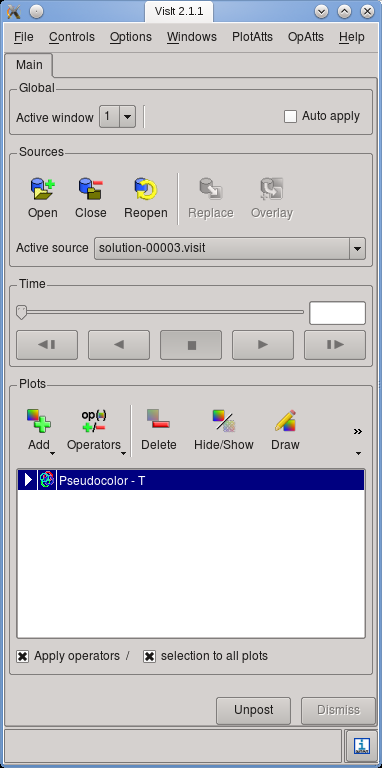
\includegraphics[width=0.24\textwidth]{viz/visit/visit-2.png}
    \label{fig:visit-1:b}
  }
  \hfill
  \subfigure[]{
    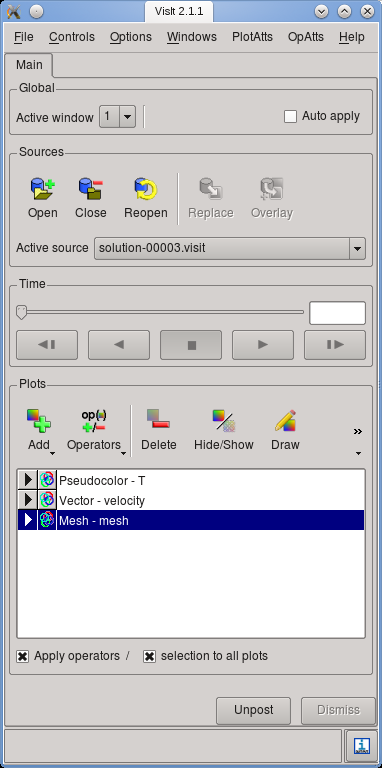
\includegraphics[width=0.24\textwidth]{viz/visit/visit-3.png}
    \label{fig:visit-1:c}
  }
  \hfill
  \phantom{.}
  \caption{\it Main window of Visit, illustrating the different steps of
    adding content to a visualization.}
  \label{fig:visit-1}
\end{figure}

\begin{figure}[tbp]
  \phantom{.}
  \hfill
  \subfigure[]{
    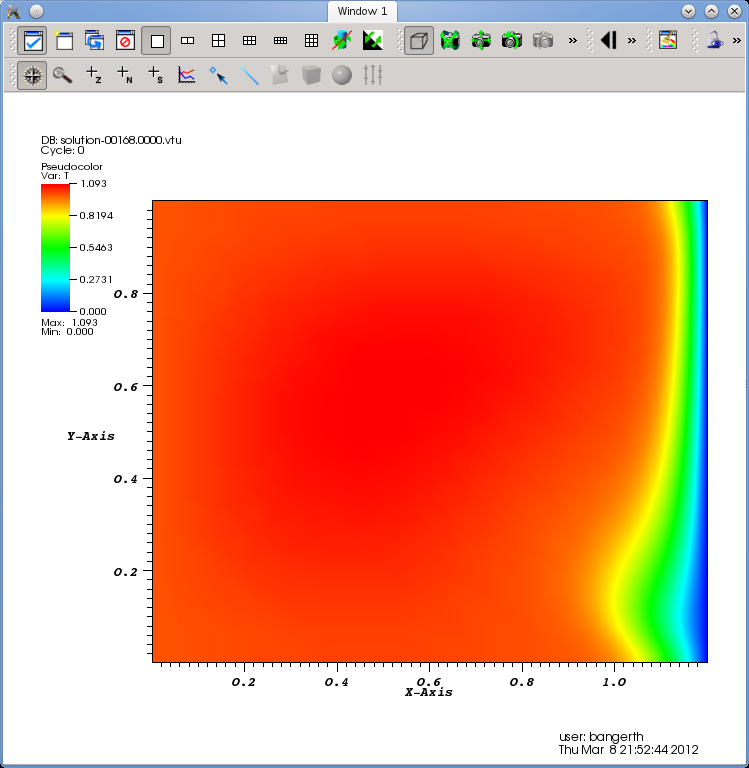
\includegraphics[width=0.48\textwidth]{viz/visit/visit-4.png}
    \label{fig:visit-2:a}
  }
  \hfill
  \subfigure[]{
    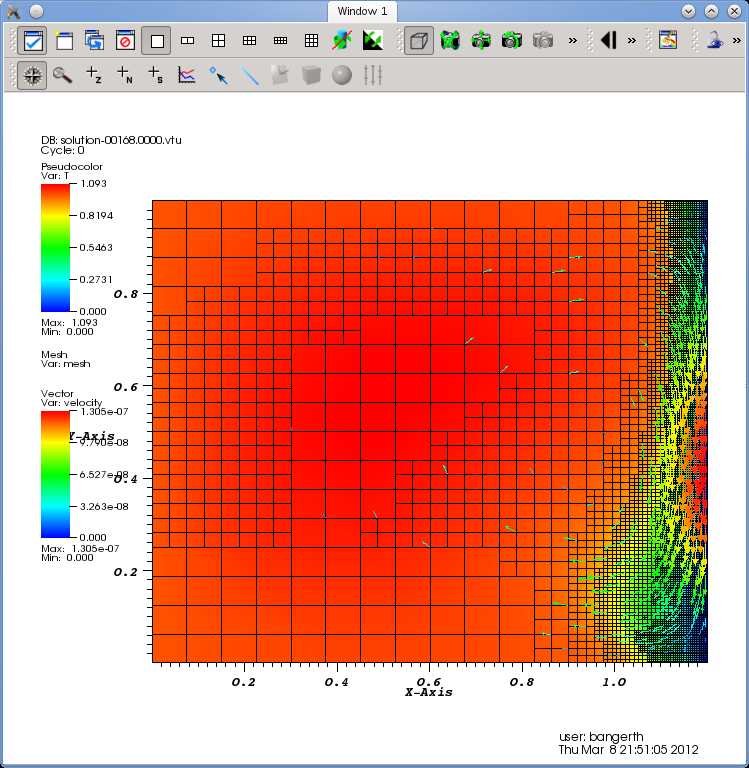
\includegraphics[width=0.48\textwidth]{viz/visit/visit-5.png}
    \label{fig:visit-2:b}
  }
  \hfill
  \phantom{.}
  \caption{\it Display window of Visit, showing a single plot and one where
    different data is overlaid.}
  \label{fig:visit-2}
\end{figure}

\begin{itemize}
\item \textit{Selecting input files:} As mentioned above, in parallel
  computations we usually generate one output file per processor in each time
  step for which visualization data is produced (see, however,
  Section~\ref{sec:viz-data}). To tell Visit which files together make up one
  time step, \aspect{} creates a \texttt{output/solution/solution-XXXXX.visit}
  file in the output directory. To open it, start Visit, click on the ``Open'' button in
  the ``Sources'' area of
  its main window (see Fig.~\ref{fig:visit-1:a}) and select the file you
  want. Alternatively, you can also select files using the ``File $>$ Open''
  menu item, or hit the corresponding keyboard short-cut. After adding an
  input source, the ``Sources'' area of the main window should list the
  selected file name. More easily, you can also just open
  \texttt{output/solution.visit} which references \textit{all} output files for
  all time steps. If you open this, Visit will display a slider that allows you
  to select which time step you want to visualize, along with forward, backward,
  and play buttons that allow you to move between time steps.

\item \textit{Selecting what to plot:} \aspect{} outputs all sorts of
  quantities that characterize the solution, such as temperature, pressure,
  velocity, and many others on demand (see
  Section~\ref{parameters:Postprocess/Visualization}). Once an input file has
  been opened, you will want to add graphical representations of some of this
  data to the still empty canvas. To this end, click on the ``Add'' button of
  the ``Plots'' area. The resulting menu provides a number of different kinds
  of plots. The most important for our purpose are: (i) ``Pseudocolor'' allows
  the visualization of a scalar field (e.g., temperature, pressure, density)
  by using a color field. (ii) ``Vector'' displays a vector-valued field
  (e.g., velocity) using arrows. (iii) ``Mesh'' displays the mesh. The
  ``Contour'', ``Streamline'' and ``Volume'' options are also frequently
  useful, in particular in 3d.

  Let us choose the ``Pseudocolor'' item and select the temperature field as
  the quantity to plot. Your main window should now look as shown in
  Fig.~\ref{fig:visit-1:b}. Then hit the ``Draw'' button to make Visit generate
  data for the selected plots. This will yield a picture such as shown in
  Fig.~\ref{fig:visit-2:a} in the display window of Visit.

\item \textit{Overlaying data:} Visit can overlay multiple plots in the same
  view. To this end, add another plot to the view using again the ``Add''
  button to obtain the menu of possible plots, then the ``Draw'' button to
  actually draw things. For example, if we add velocity vectors and the mesh,
  the main window looks as in Fig.~\ref{fig:visit-1:c} and the main view as in
  Fig.~\ref{fig:visit-2:b}.

\item \textit{Adjusting how data is displayed:} Without going into too much
  detail, if you double click onto the name of a plot in the ``Plots'' window,
  you get a dialog in which many of the properties of this plot can be
  adjusted. Further details can be changed by using ``Operators'' on a plot.

\item \textit{Making the output prettier:} As can be seen in
  Fig.~\ref{fig:visit-2}, Visit by default puts a lot of clutter around the
  figure -- the name of the user, the name of the input file, color bars, axes
  labels and ticks, etc. This may be useful to explore data in the beginning
  but does not yield good pictures for presentations or publications. To
  reduce the amount of information displayed, go to the ``Controls $>$
  Annotations'' menu item to get a dialog in which all of these displays can
  be selectively switched on and off.

\item \textit{Saving figures:} To save a visualization into a file that can
  then be included into presentations and publications, go to the menu item
  ``File $>$ Save window''. This will create successively numbered files in
  the directory from which Visit was started each time a view is saved. Things
  like the format used for these files can be chosen using the ``File $>$ Set
  save options'' menu item. We have found that one can often get better
  looking pictures by selecting the ``Screenshot'' method in this dialog.
\end{itemize}

More information on all of these topics can be found in the Visit
documentation, see \url{https://visit.llnl.gov/}. We have also recorded
video lectures demonstrating this process interactively at
\url{http://www.youtube.com/watch?v=3ChnUxqtt08} for Visit, and at
\url{http://www.youtube.com/watch?v=w-65jufR-bc} for ParaView.


\subsubsection{Visualizing statistical data}
\label{sec:viz-stat}

In addition to the graphical output discussed above, \aspect{} produces a
statistics file that collects information produced during each time step.
For the remainder of this section, let us assume that we have run \aspect{}
with the input file discussed in Section~\ref{sec:cookbooks-simple-box},
simulating convection in a box. After running \aspect{}, you will find
a file called \texttt{statistics} in the output directory that, at the time
of writing this, looked like this:
This file has a structure that looks (at the time of writing this section)
like this:
\begin{lstlisting}[frame=single,language=ksh,showstringspaces=false]
# 1: Time step number
# 2: Time (seconds)
# 3: Number of mesh cells
# 4: Number of Stokes degrees of freedom
# 5: Number of temperature degrees of freedom
# 6: Iterations for temperature solver
# 7: Iterations for Stokes solver
# 8: Velocity iterations in Stokes preconditioner
# 9: Schur complement iterations in Stokes preconditioner
# 10: Time step size (seconds)
# 11: RMS velocity (m/s)
# 12: Max. velocity (m/s)
# 13: Minimal temperature (K)
# 14: Average temperature (K)
# 15: Maximal temperature (K)
# 16: Average nondimensional temperature (K)
# 17: Outward heat flux through boundary with indicator 0 ("left") (W)
# 18: Outward heat flux through boundary with indicator 1 ("right") (W)
# 19: Outward heat flux through boundary with indicator 2 ("bottom") (W)
# 20: Outward heat flux through boundary with indicator 3 ("top") (W)
# 21: Visualization file name
 0 0.0000e+00 256 2467 1089  0 29 30 29 1.2268e-02 1.79026783e+00 2.54322608e+00
 1 1.2268e-02 256 2467 1089 32 29 30 30 3.7388e-03 5.89844152e+00 8.35160076e+00
 2 1.6007e-02 256 2467 1089 20 28 29 29 2.0239e-03 1.09071922e+01 1.54298908e+01
 3 1.8031e-02 256 2467 1089 15 27 28 28 1.3644e-03 1.61759153e+01 2.28931189e+01
 4 1.9395e-02 256 2467 1089 13 26 27 27 1.0284e-03 2.14465789e+01 3.03731397e+01
 5 2.0424e-02 256 2467 1089 11 25 26 26 8.2812e-04 2.66110761e+01 3.77180480e+01
 \end{lstlisting}

In other words, it first lists what the individual columns mean with a hash
mark at the beginning of the line and then has one line for each time step
in which the individual columns list what has been explained above.%
\footnote{With
  input files that ask for initial adaptive refinement, the first time step may
  appear twice because we solve on a mesh
  that is globally refined and we then start the entire computation
  over again on a once adaptively refined mesh (see the parameters in
  Section~\ref{parameters:Mesh_20refinement} for how to do that).}

This file is easy to visualize. For example, one can import it as a whitespace
separated file into a spreadsheet such as Microsoft Excel or OpenOffice/LibreOffice
Calc and then generate graphs of one column against another. Or, maybe simpler,
there is a multitude of simple graphing programs that do not need the overhead
of a full fledged spreadsheet engine and simply plot graphs. One that is
particularly simple to use and available on every major platform is \texttt{Gnuplot}.
It is extensively documented at \url{http://www.gnuplot.info/}.

\texttt{Gnuplot} is a command line program in which you enter commands that
plot data or modify the way data is plotted. When you call it, you will first
get a screen that looks like this:
\begin{lstlisting}[frame=single,showstringspaces=false]
/home/user/aspect/output gnuplot

        G N U P L O T
        Version 4.6 patchlevel 0    last modified 2012-03-04
        Build System: Linux x86_64

        Copyright (C) 1986-1993, 1998, 2004, 2007-2012
        Thomas Williams, Colin Kelley and many others

        gnuplot home:     http://www.gnuplot.info
        faq, bugs, etc:   type "help FAQ"
        immediate help:   type "help"  (plot window: hit 'h')

Terminal type set to 'qt'
gnuplot>
\end{lstlisting}
At the prompt on the last line, you can then enter commands. Given the
description of the individual columns given above, let us first try to
plot the heat flux through boundary 2 (the bottom
boundary of the box), i.e., column 19, as a function of time (column 2).
This can be achieved using the following command:
\begin{lstlisting}[frame=single,language=gnuplot,showstringspaces=false]
  plot "statistics" using 2:19
\end{lstlisting}
The left panel of Fig.~\ref{fig:viz-gnuplot-1} shows what \texttt{Gnuplot}
will display in its output window. There are many things one can
configure in these plots (see the \texttt{Gnuplot} manual referenced above).
For example, let us assume that we want to add labels to the $x$- and $y$-axes,
use not just points but lines and points for the curves,
restrict the time axis to the range $[0,0.2]$ and the heat flux axis to
$[-10:10]$,
plot not only the flux through the bottom but also through the top boundary
(column 20) and finally add a key to the figure, then the following
commands achieve this:
\begin{lstlisting}[frame=single,language=gnuplot,showstringspaces=false]
  set xlabel "Time"
  set ylabel "Heat flux"
  set style data linespoints
  plot [0:0.2][-10:10] "statistics" using 2:19 title "Bottom boundary", \
                       "statistics" using 2:20 title "Top boundary"
\end{lstlisting}
If a line gets too long, you can continue it by ending it in a backslash as
above. This is rarely used on the command line but useful when writing the
commands above into a script file, see below. We have done it here to get
the entire command into the width of the page.

\begin{figure}
  \centering
  \phantom.
  \hfill
  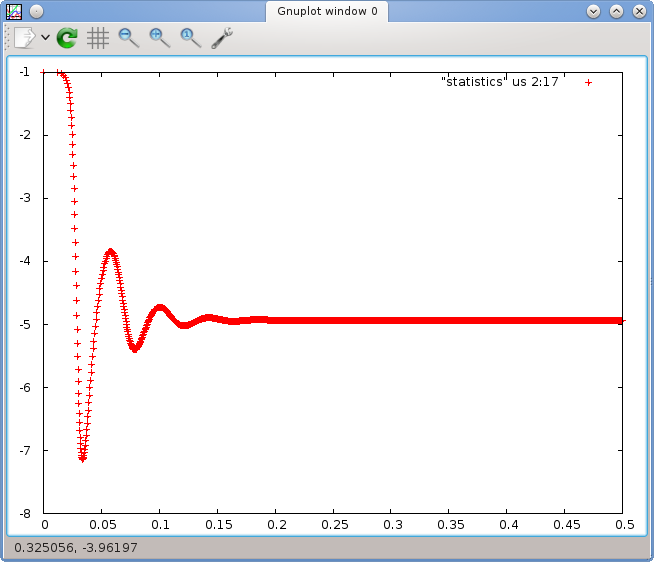
\includegraphics[width=0.4\textwidth]{viz/statistics/1.png}
  \hfill
  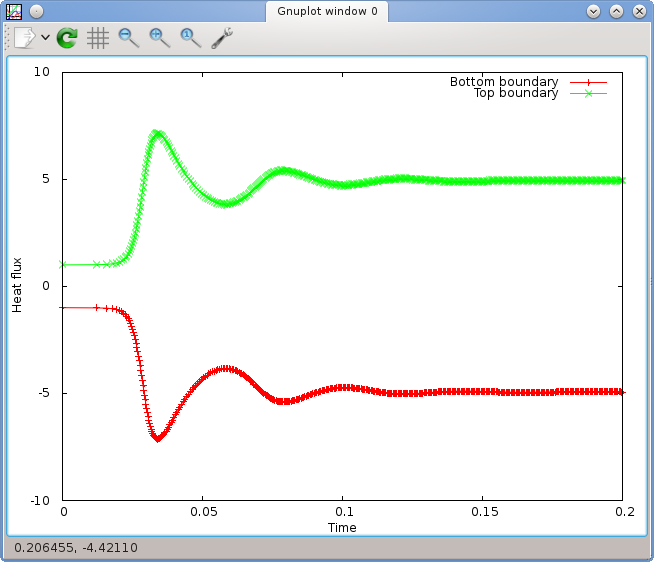
\includegraphics[width=0.4\textwidth]{viz/statistics/2.png}
  \hfill
  \phantom.
  \caption{\it Visualizing the statistics file obtained from the example in
    Section~\ref{sec:cookbooks-simple-box} using \texttt{Gnuplot}: Output
    using simple commands.}
  \label{fig:viz-gnuplot-1}
\end{figure}

For those who are lazy, \texttt{Gnuplot} allows to abbreviate things in many
different ways. For example, one can abbreviate most commands. Furthermore,
one does not need to repeat the name of an input file if it is the same
as the previous one in a plot command. Thus, instead of the commands above,
the following abbreviated form would have achieved the same effect:
\begin{lstlisting}[frame=single,language=gnuplot,showstringspaces=false]
  se xl "Time"
  se yl "Heat flux"
  se sty da lp
  pl [:0.2][-10:10] "statistics" us 2:19 t "Bottom boundary", "" us 2:20 t "Top boundary"
\end{lstlisting}
This is of course unreadable at first but becomes useful once you become
more familiar with the commands offered by this program.

Once you have gotten the commands that create the plot you want right, you probably
want to save it into a file. \texttt{Gnuplot} can write output in many
different formats. For inclusion in publications, either \texttt{eps} or
\texttt{png} are the most common. In the latter case, the commands to
achieve this are
\begin{lstlisting}[frame=single,language=gnuplot,showstringspaces=false]
  set terminal png
  set output "heatflux.png"
  replot
\end{lstlisting}
The last command will simply generate the same plot again but this time
into the given file. The result is a graphics file similar to the one
shown in Fig.~\ref{fig:convection-box-stats} on page \pageref{fig:convection-box-stats}.

\note{After setting output to a file, \textit{all} following plot commands will
  want to write to this file. Thus, if you want to create more plots after
  the one just created, you need to reset output back to the screen. On Linux,
  this is done using the command \texttt{set terminal X11}. You can then
  continue experimenting with plots and when you have the next plot ready,
  switch back to output to a file.}

What makes \texttt{Gnuplot} so useful is that it doesn't just allow entering
all these commands at the prompt. Rather, one can write them all into a file,
say \texttt{plot-heatflux.gnuplot}, and then, on the command line, call
\begin{lstlisting}[frame=single,language=ksh]
  gnuplot plot-heatflux.gnuplot
\end{lstlisting}
to generate the \texttt{heatflux.png} file. This comes in handy if one wants
to create the same plot for multiple simulations while playing with parameters
of the physical setup. It is also a very useful tool if one wants to generate
the same kind of plot again later with a different data set, for example when
a reviewer requested additional computations to be made for a paper or if one
realizes that one has forgotten or misspelled an axis label in a plot.%
\footnote{In my own work, I usually save the \aspect{} input file, the
  \texttt{statistics} output file and the \texttt{Gnuplot} script along with
  the actual figure I want to include in a paper. This way, it is easy to
  either re-run an entire simulation, or just tweak the graphic at a later
  time. Speaking from experience, you will not believe how often one wants
  to tweak a figure long after it was first created. In such situations it is
  outstandingly helpful if one still has both the actual data as well as the script
  that generated the graphic.}

\texttt{Gnuplot} has many many more features we have not even touched upon. For
example, it is equally happy to produce three-dimensional graphics, and it also
has statistics modules that can do things like curve fits, statistical regression,
and many more operations on the data you provide in the columns of an input file.
We will not try to cover them here but instead refer to the manual at
\url{http://www.gnuplot.info/}. You can also get a good amount of information
by typing \texttt{help} at the prompt, or a command like \texttt{help plot} to
get help on the \texttt{plot} command.


\subsubsection{Large data issues for parallel computations}
\label{sec:viz-data}

Among the challenges in visualizing the results of parallel computations is
dealing with the large amount of data. The first bottleneck this presents is
during run-time when \aspect{} wants to write the visualization data of a time
step to disk. Using the compressed VTU format, \aspect{} generates on the
order of 10 bytes of output for each degree of freedom in 2d and more in 3d;
thus, output of a single time step can run into the range of gigabytes that
somehow have to get from compute nodes to disk. This stresses both the cluster
interconnect as well as the data storage array.
\index[prmindex]{Number of grouped files}
\index[prmindexfull]{Postprocess!Visualization!Number of grouped files}


There are essentially two strategies supported by \aspect{} for this scenario:
\begin{itemize}
\item If your cluster has a fast interconnect, for example Infiniband, and if
  your cluster has a fast, distributed file system, then \aspect{} can produce
  output files that are already located in the correct output directory (see
  the options in Section~\ref{parameters:global}) on the global file
  system. \aspect{} uses MPI I/O calls to this end, ensuring that the local
  machines do not have to access these files using slow NFS-mounted global
  file systems.

\item If your cluster has a slow interconnect, e.g., if it is simply a
  collection of machines connected via Ethernet, then writing data to a
  central file server may block the rest of the program for a while. On the
  other hand, if your machines have fast local storage for temporary file
  systems, then \aspect{} can write data first into such a file and then move
  it in the background to its final destination while already continuing
  computations. To select this mode, set the appropriate variables discussed
  in Section~\ref{parameters:Postprocess/Visualization}. Note, however, that
  this scheme only makes sense if every machine on which MPI processes run has
  fast local disk space for temporary storage.
\end{itemize}

\note{An alternative would be if every processor directly writes its own files
  into the global output directory (possibly in the background), without the
  intermediate step of the temporary file. In our experience, file servers are
  quickly overwhelmed when encountering a few hundred machines wanting to
  open, fill, flush and close their own file via NFS mounted file system
  calls, sometimes completely blocking the entire cluster environment for
  extended periods of time.}

\subsection{Checkpoint/restart support}
\label{sec:checkpoint-restart}

If you do long runs, especially when using parallel computations, there are a
number of reasons to periodically save the state of the program:
\begin{itemize}
\item If the program crashes for whatever reason, the entire computation may
  be lost. A typical reason is that a program has exceeded the requested
  wallclock time allocated by a batch scheduler on a cluster.
\item Most of the time, no realistic initial conditions for strongly
  convecting flow are available. Consequently, one typically starts with a
  somewhat artificial state and simply waits for a long while till the
  convective state enters the phase where it shows its long-term
  behavior. However, getting there may take a good amount of CPU time and it
  would be silly to always start from scratch for each different parameter
  setting. Rather, one would like to start such parameter studies with a saved
  state that has already passed this initial, unphysical, transient stage.
\end{itemize}

To this end, \aspect{} creates a set of files in the output directory
\index[prmindex]{Output directory}
\index[prmindexfull]{Output directory}
(selected in the parameter file) every N time steps (controlled by the number
of steps or wall time as specified in \texttt{subsection Checkpointing}, see
Section~\ref{parameters:Checkpointing}) in which the entire state of the
program is saved so that a simulation can later be continued at this
point. The previous checkpoint files will then be deleted. To resume
operations from the last saved state, you need to set the \texttt{Resume
  computation} flag in the input parameter file to \texttt{true}, see
\index[prmindex]{Resume computation}
\index[prmindexfull]{Resume computation}
Section~\ref{parameters:Resume computation}.

\note{It is not imperative that the parameters selected in the input file are
  exactly the same when resuming a program from a saved state than what they
  were at the time when this state was saved. For example, one may want to
  choose a different parameterization of the material law, or add or remove
  postprocessors that should be run at the end of each time step. Likewise,
  the end time, the times at which some additional mesh refinement steps
  should happen, etc., can be different.

  Yet, it is
  clear that some other things can't be changed: For example, the geometry
  model that was used to generate the coarse mesh and describe the boundary
  must be the same before and after resuming a computation. Likewise, you can
  not currently restart a computation with a different number of processors
  than initially used to checkpoint the simulation.
  Not all invalid
  combinations are easy to detect, and \aspect{} may not always realize
  immediate what is going on if you change a setting that can't be
  changed. However, you will almost invariably get nonsensical results after
  some time.}


\subsection{Making \aspect{} run faster}

When developing \aspect{}, we are guided by the principle that the default for
all settings should be \textit{safe}. In particular, this means that you should
get errors when something goes wrong, the program should not let you choose an
input file parameter so that it doesn't make any sense, and we should solve the
equations to best ability without cutting corners. The goal is that when you
start working with \aspect{} that we give you the best answer we can. The
downside is that this also makes \aspect{} run slower than may be possible. This
section describes ways of making \aspect{} run faster -- assuming that you know
what you are doing and are making conscious decisions.

\subsubsection{Debug vs.~optimized mode}
Both \dealii{} and \aspect{} by default have a great deal of internal checking
to make sure that the code's state is valid. For example, if you write a new
postprocessing plugin (see Section~\ref{sec:plugins})) in which you need to
access the solution vector, then \dealii{}'s \texttt{Vector} class will make
sure that you are only accessing elements of the vector that actually exist and
are available on the current machine if this is a parallel computation. We do so
because it turns out that by far the most bugs one introduces in programs are of
the kind where one tries to do something that obviously doesn't make sense
(such as accessing vector element 101 when it only has 100 elements). These
kinds of bugs are more frequent than implementing a wrong algorithm, but they
are fortunately easy to find if you have a sufficient number of assertions in
your code. The downside is that assertions cost run time.

As mentioned above, the default is to have all of these assertions in the code
to catch those places where we may otherwise silently access invalid memory
locations. However, once you have a plugin running and verified that your input
file runs without problems, you can switch off all of these checks by switching
from debug to optimized mode. This means re-compiling \aspect{} and linking
against a version of the \dealii{} library without all of these internal checks.
Because this is the first thing you will likely want to do, we have already
discussed how to do all of this in Section~\ref{sec:debug-mode}.

\subsubsection{Adjusting solver tolerances} At the heart of every time step
lies the solution of linear systems for the Stokes equations, the temperature
field, and possibly for compositional fields. In essence, each of these steps
requires us to solve a linear system of the form $Ax=b$ which we do through
iterative solvers, i.e., we try to find a sequence of approximations $x^{(k)}$
where $x^{(k)}\rightarrow x=A^{-1}b$. This iteration is terminated at iteration
$k$ if the approximation is ``close enough'' to the exact solution. The solvers
we use determine this by testing after every iteration whether the
\textit{residual}, $r^{(k)}=A(x-x^{(k)})=b-Ax^{(k)}$, satisfies
$\|r^{(k)}\|\le\varepsilon\|r^{(0)}\|$ where $\varepsilon$ is called the
(relative) \textit{tolerance}.

Obviously, the smaller we choose $\varepsilon$, the more accurate the
approximation $x^{(k)}$ will be. On the other hand, it will also take more
iterations and, consequently, more CPU time to reach the stopping criterion with
a smaller tolerance. The default value of these tolerances are chosen so that
the approximation is typically sufficient. You can make \aspect{} run faster if
you choose these tolerances larger.
The parameters you can adjust are all listed in
Section~\ref{parameters:Solver_20parameters} and are located in the \texttt{Solver parameters} subsection of the input
file. In particular, the parameters you want to look at are \texttt{Linear
solver tolerance}, \texttt{Temperature solver tolerance} and
\texttt{Composition solver tolerance}.
\index[prmindex]{Composition solver tolerance}
\index[prmindexfull]{Composition solver tolerance}
\index[prmindex]{Linear solver tolerance}
\index[prmindexfull]{Linear solver tolerance}
\index[prmindex]{Temperature solver tolerance}
\index[prmindexfull]{Temperature solver tolerance}

All this said, it is important to understand the consequences of choosing
tolerances larger. In particular, if you choose tolerances too large, then the
difference between the exact solution of a linear system $x$ and the
approximation $x^{(k)}$ may become so large that you do not get an accurate
output of your model any more. A rule of thumb in choosing tolerances is to
start with a small value and then increase the tolerance until you come to a
point where the output quantities start to change significantly. This is the
point where you will want to stop.

\subsubsection{Adjusting solver preconditioner tolerances} To solve the Stokes
equations it is necessary to lower the condition number of the
Stokes matrix by preconditioning  it. In \aspect{} a right preconditioner $Y^{-1} =
\begin{pmatrix}
\widetilde{A^{-1}} & -\widetilde{A^{-1}}B^{T}\widetilde{S^{-1}} \\
0 & \widetilde{S^{-1}}
\end{pmatrix}$ is used to precondition the system, where $\widetilde{A^{-1}}$ is
the approximate inverse of the A block and $\widetilde{S^{-1}}$ is the approximate
inverse of the Schur complement matrix. Matrix $\widetilde{A^{-1}}$ and
$\widetilde{S^{-1}}$ are calculated through a CG solve, which requires a tolerance
to be set. In comparison with the solver tolerances of the previous section, these
parameters are relatively safe to use, since they only change the preconditioner,
but can speed up or slow down solving the Stokes system considerably.

In practice $\widetilde{A^{-1}}$ takes by far the most time to compute, but is
also very important in conditioning the system. The accuracy of the computation
of $\widetilde{A^{-1}}$ is controlled by the parameter \texttt{Linear solver A
block tolerance} which has a default value of $1e-2$. Setting this tolerance
to a less strict value will result in more outer iterations, since the
preconditioner is not as good, but the amount of time to compute
$\widetilde{A^{-1}}$ can drop significantly resulting in a reduced total solve
time. The cookbook crustal deformation (Section
\ref{sec:cookbooks-crustal-deformation}) for example can be computed much faster
by setting the \texttt{Linear solver A block tolerance} to $5e-1$. The
calculation of $\widetilde{S^{-1}}$ is usually much faster and the
conditioning of the system is less sensitive to the parameter \texttt{Linear
solver S block tolerance}, but for some problems it might be worth it to
investigate.
\index[prmindex]{Linear solver A block tolerance}
\index[prmindexfull]{Linear solver A block tolerance}
\index[prmindex]{Linear solver S block tolerance}
\index[prmindexfull]{Linear solver S block tolerance}

\subsubsection{Using lower order elements for the temperature/compositional discretization}
The default settings of \aspect{} use quadratic finite elements for the
velocity. Given that the temperature and compositional fields essentially (up
to material parameters) satisfy advection equations of the kind $\partial_t T +
\mathbf u \cdot \nabla T = \ldots$, it seems appropriate to also use quadratic
finite element shape functions for the temperature and compositional fields.

However, this is not mandatory. If you do not care about high accuracy in these
fields and are mostly interested in the velocity or pressure field, you can
select lower-order finite elements in the input file. The polynomial degrees are
controlled with the parameters in the \textit{discretization} section of the
input file, see Section~\ref{parameters:Discretization}, in particular by
\texttt{Temperature polynomial degree} and
\texttt{Composition polynomial degree}.
\index[prmindex]{Temperature polynomial degree}
\index[prmindexfull]{Discretization!Temperature polynomial degree}
\index[prmindex]{Composition polynomial degree}
\index[prmindexfull]{Discretization!Composition polynomial degree}

As with the other parameters discussed above and below, it is worthwhile
comparing the results you get with different values of these parameters when
making a decision whether you want to save on accuracy in order to reduce
compute time. An example of how this choice affects the accuracy you get is
discussed in Section~\ref{sec:cookbooks-simple-box}.



\subsubsection{Limiting postprocessing}
\aspect{} has a lot of postprocessing capabilities, from generating graphical
output to computing average temperatures or temperature fluxes. To see what all
is possible, take a look at the \texttt{List of postprocessors} parameter that
can be set in the input file, see Section~\ref{parameters:Postprocess}.
\index[prmindex]{List of postprocessors}
\index[prmindexfull]{Postprocess!List of postprocessors}

Many of these postprocessors take a non-negligible amount of time. How much they
collectively use can be inferred from the timing report \aspect{} prints
periodically among its output, see for example the output shown in
Section~\ref{sec:cookbooks-simple-box}. So, if your computations take too long,
consider limiting which postprocessors you run to those you really need. Some
postprocessors -- for example those that generate graphical output, see
Section~\ref{parameters:Postprocess/Visualization} -- also allow you to run them
only once every once in a while, rather than at every time step.


\subsubsection{Switching off pressure normalization}
In most practically relevant cases, the Stokes equations
\eqref{eq:stokes-1}--\eqref{eq:stokes-2} only determine the pressure up to a
constant because only the pressure gradient appears in the equations, not the
actual value of it. However, unlike this ``mathematical'' pressure, we have a
very specific notion of the ``physical'' pressure: namely a well-defined
quantity that at the surface of Earth equals the air pressure, which compared to
the hydrostatic pressure inside Earth is essentially zero.

As a consequence, the default in \aspect{} is to normalize the computed
``mathematical'' pressure in such a way that either the mean pressure at the
surface is zero (where the geometry model describes where the ``surface'' is,
see Section~\ref{sec:geometry-models}), or that the mean pressure in the domain
is zero. This normalization is important if your model describes densities,
viscosities and other quantities in dependence of the pressure -- because you
almost certainly had the ``physical'' pressure in mind, not some unspecified
``mathematical'' one. On the other hand, if you have a material model in which
the pressure does not enter, then you don't need to normalize the pressure at
all -- simply go with whatever the solver provides. In that case, you can switch
off pressure normalization by looking at the \texttt{Pressure normalization}
parameter at the top level of the input file, see
Section~\ref{parameters:global}.
\index[prmindex]{Pressure normalization}
\index[prmindexfull]{Pressure normalization}


\subsubsection{Regularizing models with large coefficient variation}
Models with large jumps in viscosity and other coefficients present
significant challenges to both discretizations and solvers. In particular,
they can lead to very long solver
times. Section~\ref{sec:sinker-with-averaging} presents parameters that can
help regularize models and these typically also include significant
improvements in run-time.
\index[prmindex]{Material averaging}
\index[prmindexfull]{Material model!Material averaging}


\subsubsection{Using multithreading}
In most cases using as many MPI processes as possible is the optimal
parallelization strategy for \aspect{} models, but if you are limited by the
amount of MPI communication it can be beneficial to use multiple threads per
MPI process. While not utilized by our linear solvers, this parallelization can
speed up the assembly of the system matrices, e.g. by around 10-15\% if you
utilize unused logical cores, or nearly linearly if you use otherwise
unused physical cores. This can also reduce the performance cost if you are
memory limited and need to run your model on less than the available number of
cores per node on a cluster to increase the available memory per core.  Running
with for example two threads per process will offset some of the performance
loss you will see in these situations.

Multithreading is controlled by setting the command line parameter \texttt{-j}
or \texttt{-{}-threads}. If the parameter is not set, \aspect{} will create
exactly one thread per MPI process, i.e. multithreading is disabled.  Appending
the parameter allows \aspect{} to spawn several threads per MPI process. Note
that the internally used TBB library will determine the number of threads based
on the number of available cores, i.e., if you start 2~MPI processes on a
quadcore machine with hyperthreading (8 logical cores), \aspect{} will spawn 4
threads on each MPI process. Also note that there is no guarantee that the
final number of threads will exactly match the number of available logical
cores if you start with a number of processes that is not a divisor of your
logical cores (e.g. 3 MPI processes for 8 logical cores).

\subsection{Input parameter files}
\label{sec:parameters-overview}

What \aspect{} computes is driven by two things:
\begin{itemize}
\item The models implemented in \aspect{}. This includes the geometries, the
  material laws, or the initial conditions currently supported. Which of these
  models are currently implemented is discussed below;
  Section~\ref{sec:extending} discusses in great detail the process of
  implementing additional models.

\item Which of the implemented models is selected, and what their run-time
  parameters are. For example, you could select a model that prescribes
  constant coefficients throughout the domain from all the material models
  currently implemented; you could then select appropriate values for all of
  these constants. Both of these selections happen from a parameter file that
  is read at run time and whose name is specified on the command line. (See
  also Section~\ref{sec:running-overview}.)
\end{itemize}
In this section, let us give an overview of what can be selected in the
parameter file. Specific parameters, their default values, and allowed values
for these parameters are documented in Section~\ref{sec:parameters}. An index
with page numbers for all run-time parameters can be found on
page~\pageref{sec:runtime-parameter-index}.

\subsubsection{The structure of parameter files}

Most of the run-time behavior of \aspect{} is driven by a parameter file that
looks in essence like this:
\lstinputlisting[language=prmfile]{cookbooks/overview/doc/structure.part.prm.out}

Some parameters live at the top level, but most parameters are grouped into
subsections. An input parameter file is therefore much like a file system: a
few files live in the root directory; others are in a nested hierarchy of
sub-directories. And just as with files, parameters have both a name (the
thing to the left of the equals sign) and a content (what's to the right).

All parameters you can list in this input file have been \textit{declared} in
\aspect. What this means is that you can't just list anything in the input
file, and expect that entries that are unknown are simply ignored.
Rather, if your input file contains a line setting a parameter that is unknown, you
will get an error message. Likewise, all declared parameters have a
description of possible values associated with them -- for example, some
parameters must be non-negative integers (the number of initial refinement
steps), can either be true or false (whether the computation should be resumed
from a saved state), or can only be a single element from a selection (the
name of the material model). If an entry in your input file doesn't satisfy
these constraints, it will be rejected at the time of reading the file (and
not when a part of the program actually accesses the value and the programmer
has taken the time to also implement some error checking at this location).
Finally, because parameters have been declared, you do not \textit{need} to
specify a parameter in the input file: if a parameter isn't listed, then the
program will simply use the default provided when declaring the parameter.

\note{In cases where a parameter requires a significant amount of text, you can
end a line in the input file with a backslash. This indicates that the
following line will simply continue to be part of the text of the current line,
in the same way as the C/C++ preprocessor expands lines that end in
backslashes. The underlying implementation always eats whitespace at
the beginning of each continuing line, but not before the
backslash. This means that the parameter file \\
\hspace*{.25cm} \texttt{set Some parameter = abc}$\backslash$ \\
\hspace*{.25cm} \texttt{\phantom{set Some parameter = }def}\\
is equivalent to \\
\hspace*{.25cm} \texttt{set Some parameter = abcdef}\\
that is, with no space between \texttt{abc} and \texttt{def} despite
the leading whitespace at the beginning of the second line. If you
do want space between these two parts, you need to add it before the
backslash in the first of the two lines.
}

\subsubsection{Categories of parameters}

The parameters that can be provided in the input file can roughly be
categorized into the following groups:
\begin{itemize}
\item Global parameters (see Section~\ref{parameters:global}): These
  parameters determine the overall behavior of the program. Primarily they
  describe things like the output directory, the end time of the simulation,
  or whether the computation should be resumed from a previously saved state.

\item Parameters for certain aspects of the numerical algorithm: These
  describe, for example, the specifics of the spatial discretization. In
  particular, this is the case for parameters concerning
  the polynomial degree of the finite element approximation
  (Section~\ref{parameters:Discretization}), some details about the
  stabilization
  (Section~\ref{parameters:Discretization/Stabilization_20parameters}), and
  how adaptive mesh refinement is supposed to work
  (Section~\ref{parameters:Mesh_20refinement}).

\item Parameters that describe certain global aspects of the equations to be
  solved: This includes, for example, a description if certain terms in the
  model should be omitted or not. See
  Section~\ref{parameters:Formulation} for the list of parameters in this
  category.

\item Parameters that characterize plugins: Certain behaviors of
  \aspect{} are described by what we call \textit{plugins} -- self-contained
  parts of the code that describe one particular aspect of the simulation. An
  example would be which of the implemented material models to use, and the
  specifics of this material model. The sample parameter file above gives an
  indication of how this works: within a subsection of the file that pertains
  to the material models, one can select one out of several plugins (or, in
  the case of the postprocessors, any number, including none, of the available
  plugins), and one can then specify the specifics of this model in a
  sub-subsection dedicated to this particular model.

  A number of components of \aspect{} are implemented via plugins. Some of
  these, together with the sections in which their parameters are declared, are
  the following:
  \begin{itemize}
  \item The material model:
    Sections~\ref{parameters:Material_20model} and following.
  \item The geometry:
    Sections~\ref{parameters:Geometry_20model} and following.
  \item The gravity description:
    Sections~\ref{parameters:Gravity_20model} and following.
  \item Initial conditions for the temperature:
    Sections~\ref{parameters:Initial_20temperature_20model} and following.
  \item Temperature boundary conditions:
    Sections~\ref{parameters:Boundary_20temperature_20model} and following.
  \item Postprocessors:
    Sections~\ref{parameters:Postprocess} and following for most postprocessors,
    section \ref{parameters:Postprocess/Visualization} and following for
    postprocessors related to visualization.
  \end{itemize}
\end{itemize}

The details of parameters in each of these categories can be found in the
sections linked to above. Some of them will also be used in the cookbooks in
Section~\ref{sec:cookbooks}.


\subsubsection{A note on the syntax of formulas in input files}
\label{sec:muparser-format}

Input files have different ways of describing certain things to \aspect{}. For
example, you could select a plugin for the temperature initial values that
prescribes a constant temperature, or a
plugin that implements a particular formula for these initial conditions in
C++ in the code of the plugin, or a
plugin that allows you to describe this formula in a symbolic way in the input file
(see Section~\ref{parameters:Initial_20temperature_20model}). An example of this latter
case is this snippet of code discussed in
Section~\ref{sec:cookbooks-simple-box-3d}:
%
\lstinputlisting[language=prmfile]{cookbooks/convection_box_3d/doc/initial.part.prm.out}
%
The formulas you can enter here need to use a syntax that is understood by the
functions and classes that interpret what you write. Internally, this is done
using the muparser library, see \url{http://muparser.beltoforion.de/}. The
syntax is mostly self-explanatory in that it allows to use the usual symbols
\texttt{x}, \texttt{y} and \texttt{z} to reference coordinates (unless a
particular plugin uses different variables, such as the depth), the symbol
\texttt{t} for time in many situations, and allows you to use all of the
typical mathematical functions such as sine and cosine. Based on the muparser
library, deal.II supports additional functions, including \texttt{|} (the logical OR), \texttt{\&} (the logical AND),
\texttt{int()}, \texttt{ceil()}, \texttt{floor()}, \texttt{cot()},
\texttt{csc()}, \texttt{sec()}, \texttt{pow()}, \texttt{log()},
\texttt{erfc()}, \texttt{rand()}, and \texttt{rand\_seed()}.
For more detailed information, see
\url{http://www.dealii.org/developer/doxygen/deal.II/classFunctionParser.html#details}.

A common need for function expression is an if-else-statement, for example
``if $1<x<4$ then output 1, else output 0''.
The muparser uses lazy-expression syntax \texttt{(if-condition ?\ true-expression :\ false-expression )}
for if-else statements. This lazy-expression only evaluates the expression that meets the
if-condition, rather than evaluating both expressions, which can be useful if one of the
expressions is not defined (e.g., has a divide by zero) when the if-condition is not met.
Note it is also possible to use the syntax \texttt{if(condition, true-expression, false-expression)},
but in this case both expressions are always evaluated. This is inefficient, but in addition may abort the program with a floating point exception if the expression that will be discarded has invalid floating point operations (such as a division by zero, or taking the square root of a negative number) that would ordinarily not be visible because, after all, the expression should be discarded.
Therefore, the lazy-expression syntax is recommended.

As a simple example using the lazy-expression syntax, the statement ``if $1<x<4$ then output 1, else output 0''
can be expressed as \texttt{(1<x\ \&\&\ x<4 ?\ 1\ :\ 0)}.  Multiple, nested if-else expressions
can also be used. To extend the simple example, the statement
``if $1<x<4$ then, if 2<y<3, then output 2, else output 1, else output 0''
can be expressed as \texttt{((1<x\ \&\&\ x<4)\ ?\ ((2<y\ \&\&\ y<3)\ ?\ 2\ :\ 1)\ :\ (0))}.

An example for how to translate nested if-else statements into the lazy-expression syntax is given in the
cookbook example found in Section~\ref{sec:lazy-expression}. This cookbook includes a python script that defines
the initial temperature structure using nested if-else statements and shows how this is then rewritten
using the lazy-expression. The cookbook runs a single time-step to show the outcome of using the function
option for the initial temperature. Quite complex initial conditions can be defined in this way, however,
using something like python to debug these expressions before defining them in the parameter file is
recommended. For more examples of functions used in parameter files, go to the \texttt{cookbooks}
directory and use grep to search for ``Function expression'' in the parameters files.
You can also search ``Function expression'' on the \aspect{} github page.
For more examples of the syntax understood, reference the documentation of the muparser library
linked to above.

\subsubsection{Compatibility of input files with newer \aspect{} versions}

We strive to maintain compatibility for options in input files as long as
possible. However, occasionally we have to reorder, rename, or remove options
from parameter files to improve \aspect{} further. This is especially true
for new major versions. In order to allow running old parameter files with
newer \aspect{} versions we provide scripts that can automatically update
existing parameter files to the new syntax. Executing
\texttt{doc/update\_prm\_files.sh} with one or more parameter files as
arguments will create a backup of the old parameter file (named
\texttt{old\_filename.bak}), and replace the existing file with a version that
should work with the current \aspect{} version. Using this script would look
like this:

\begin{lstlisting}[frame=single,language=ksh,showstringspaces=false]
bash contrib/utilities/update_prm_files.sh cookbooks/convection_box.prm
\end{lstlisting}

\note{Not all text replacements are unique, and the structure of input files
allows for constructions the script can not properly parse. Also we can not
guarantee to preserve the structure and position of comments, as it is not
always clear to which part of the input file they refer. Thus, it is important
that you check your updated input file for errors. That being said, all input
files in the main \aspect{} repository are updated successfully using this
script.}

\subsection{A graphical user interface for editing \aspect{} parameter files}
Preparing a parameter file in a text editor can be a tedious task, not
only because the number of input parameters has grown considerably during the
development of \aspect{}, but also because remembering the names of commonly
used options is a waste of (human) memory. Therefore, we provide a graphical
user interface that builds upon an available program for \dealii{}. This GUI
allows to investigate existing input parameters, including their default values, modify
these values in a spreadsheet like environment and then save a formatted
parameter file that can be used to start an ASPECT model. In the following
subsections we describe installing and using this user interface.

\subsubsection{Installing parameter-GUI}
The \dealii{} parameter-GUI program can be downloaded at \url{https://github.com/dealii/parameter_gui},
and is compiled using the \texttt{cmake} program just like \aspect{} itself. The program has no
dependencies except for the Qt development libraries that should be available as packages for
most Linux distributions and can also be obtained for all major operating systems at
\url{https://www.qt.io/download-open-source/}.

Example steps for installing the parameter-gui could look as follows:
\begin{enumerate}
\item Download the program from \url{https://github.com/dealii/parameter_gui}.
\item Prepare a Makefile by running \texttt{cmake .} in the source folder.
\item Compile the program by running \texttt{make}.
\item Make sure to set the environment variable \texttt{PARAMETER\_GUI\_DIR}
to the directory that contains the parameter-GUI executable (optional).
This will allow \aspect{} to automatically enable the GUI during configuration.
\end{enumerate}

\paragraph{Installing on macOS} On a mac machine with recent macOS Sierra 10.12.4, Qt development libraries of version 4.x.x at the libraries' official website \url{https://www.qt.io/download-open-source/} may fail to install.  Alternatively, you can install \texttt{qt4} through Homebrew (also see instruction here \url{https://github.com/cartr/homebrew-qt4})
\begin{verbatim}
brew tap cartr/qt4
brew tap-pin cartr/qt4
brew install qt@4
\end{verbatim}
or install it through Mac Ports (\url{https://www.macports.org/})
\begin{verbatim}
sudo port install qt4-mac
\end{verbatim}
Then you can follow the Linux user instructions provided previously to download and install dealii parameter-GUI.
Before running \texttt{cmake .}, you may need to either pass the path of \texttt{qt4} and specify the value of variable \texttt{QT\_LIBRARIES} to the directory that contains the libraries of \texttt{qt4}
or add those information into your \texttt{.bash\_profile}. For example, for installation through Mac Ports, you can set the following into your \texttt{.bash\_profile}
\begin{verbatim}
export PATH="$PATH:/opt/local/libexec/qt4"
export QT_LIBRARIES="/opt/local/libexec/qt4"
\end{verbatim}




\subsubsection{Using \aspect{}-GUI}

When configuring \aspect{} after executing the above steps, it should automatically pick up the
location of the parameter-GUI, and will create a new script named \texttt{aspect-gui} within the build folder.
If this does not happen, it is possible to hand over the location of the parameter-GUI as a cmake
variable during configuration (e.g. \texttt{cmake -D PARAMETER\_GUI\_EXECUTABLE=path\_to\_your\_executable}).

The aspect-gui script can be executed from any folder either with no argument or with one argument that contains the path to
an existing parameter file. The script will run \aspect{} with the given (or an empty) parameter file, generate a database
of existing input parameters, and open the parameter-GUI program with this database. The resulting window looks similar to Fig.~\ref{fig:aspect-gui}. If an existing parameter file was
given, all parameter fields are pre-filled with the values set in the file instead of the default values.
In the program's main window you can change parameters as necessary, and then save the file as a new parameter file. This parameter file can then be used
to start an \aspect{} model as usual. Note that it is possible to prepare and execute the parameter file with different versions of \aspect{}, e.g. if you prepare parameter files on a local machine, and execute the model on a remote compute cluster.
Note however that if the two \aspect{} versions contain different default values or parameter names have changed, this can lead
to unexpected model behavior or even unusable parameter files.

\begin{figure}
\hfill
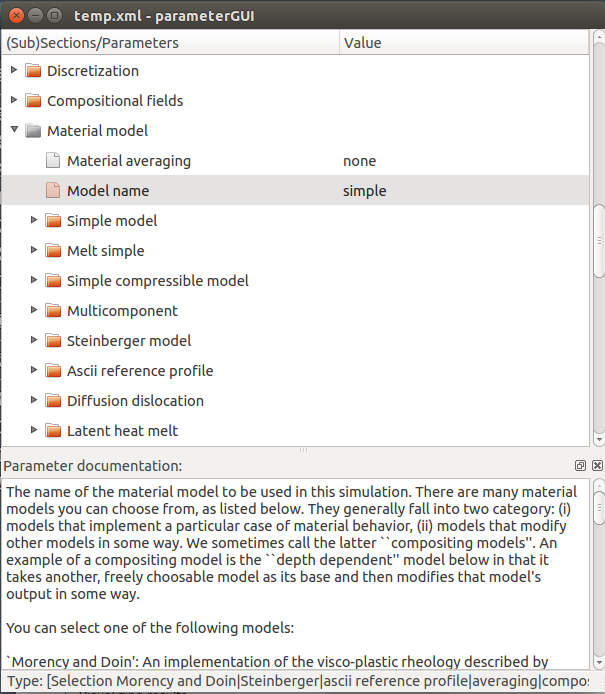
\includegraphics[width=0.4\textwidth]{aspect-gui.png}
\hfill
\phantom.
\caption{\it The parameter GUI lists all available parameter options, and allows to change and save them into a new parameter file. Input fields know about the type of the variable and will display useful options to change them (e.g. drop-down menus, file dialogs, text fields).}
\label{fig:aspect-gui}
\end{figure}

\section{Cookbooks}
\label{sec:cookbooks}

In this section, let us present a number of ``cookbooks'' -- examples of how
to use \aspect{} in typical or less typical ways. As discussed in
Sections~\ref{sec:running} and \ref{sec:parameters}, \aspect{} is driven by
run-time parameter files, and so setting up a particular situation primarily
comes down to creating a parameter file that has the right entries. Thus, the
subsections below will discuss in detail what parameters to set and to what
values. Note that parameter files need not specify \textit{all} parameters --
of which there is a bewildering number -- but only those that are relevant to
the particular situation we would like to model. All parameters not listed
explicitly in the input file are simply left at their default value (the
default values are also documented in Section~\ref{sec:parameters}).

Of course, there are situations where what you want to do is not covered by
the models already implemented. Specifically, you may want to try a different
geometry, a different material or gravity model, or different boundary
conditions. In such cases, you will need to implement these extensions in the
actual source code. Section~\ref{sec:extending} provides information on how to
do that.

The remainder of this section shows a number of applications of
\aspect{}. They are grouped into three categories: Simple setups of examples
that show thermal convection (Section~\ref{sec:cookbooks-simple}), setups
that try to model geophysical situations (Section~\ref{sec:cookbooks-geophysical})
and setups that are used to benchmark \aspect{} to ensure correctness or to test accuracy
of our solvers (Section~\ref{sec:cookbooks-benchmarks}). Before we get there,
however, we will review how one usually approaches setting up computations in
Section~\ref{sec:cookbooks-overview}.

\note{The input files discussed in the following sections can generally be
  found in the \texttt{cookbooks/} directory of your \aspect{} installation.}


\subsection{How to set up computations}
\label{sec:cookbooks-overview}

\aspect{}'s computations are controlled by input parameter files such as those
we will discuss in the following sections.%
\footnote{You can also extend \aspect{} using plugins -- i.e., pieces of code
you compile separately and either link into the \aspect{} executable itself, or
reference from the input file. This is discussed in
Section~\ref{sec:extending}.}
Basically, these are just regular text files you can edit with programs like
\texttt{gedit}, \texttt{kwrite} or \texttt{kate} when working on Linux, or
something as simple as \texttt{NotePad} on Windows. When setting up these input
files for a model you have in mind, you have to describe everything
that characterizes the situation you are considering. In particular,
this includes the following:
\begin{itemize}
  \item What internal forces act on the medium (the equation)?
  \item What external forces do we have (the right hand side)
  \item What is the domain (geometry)?
  \item What happens at the boundary for each variable involved (boundary
 conditions)?
  \item How did it look at the beginning (initial conditions)?
\end{itemize}
For each of these questions, there are one or more input parameters (sometimes
grouped into sections) that allow you to specify what you want. For example, to
choose a geometry, you will typically have a block like this in your input file:
%
\lstinputlisting[language=prmfile]{cookbooks/overview/doc/geometry.part.prm.out}
%
This indicates that you want to do a computation in 2d, using a rectangular
geometry (a ``box'') with edge length equal to one in both the $x$- and
$y$-directions. Of course, there are other geometries you can choose from for
the \texttt{Model name} parameter, and consequently other subsections that
specify the details of these geometries.

Similarly, you describe boundary conditions using parameters such as this:
%
\lstinputlisting[language=prmfile]{cookbooks/overview/doc/boundary-conditions.part.prm.out}
%
This snippet describes which of the four boundaries of the two-dimensional box
we have selected above should have a prescribed temperature or an insulating
boundary, and at which parts of the boundary we want zero, tangential or
prescribed velocities.%
\footnote{Internally, the geometry models \aspect{} uses label every part of
  the boundary with what is called a \textit{boundary indicator} -- a number
  that identifies pieces of the boundary. If you know which number each piece
  has, you can list these numbers on the right hand sides of the assignments
  of boundary types above. For example, the left boundary of the box has
  boundary indicator zero (see Section~\ref{parameters:Geometry_20model}), and
  using this number instead of the \texttt{left} would have been equally
  valid. However, numbers are far more difficult to remember than names, and
  consequently every geometry model provides string aliases such as
  ``\texttt{left}'' for each boundary indicator describing parts of the
  boundary. These symbolic aliases are specific to the geometry -- for the
  box, they are ``\texttt{left}'', ``\texttt{right}'', ``\texttt{bottom}'',
  etc., whereas for a spherical shell they are ``\texttt{inner}'' and
  ``\texttt{outer}'' -- but are described in the documentation of every
  geometry model, see Section~\ref{parameters:Geometry_20model}.}

If you go down the list of questions about the setup above, you have already
done the majority of the work describing your computation. The remaining
parameters you will typically want to specify have to do with the computation
itself. For example, what variables do you want to output and how often? What
statistics do you want to compute. The following sections will give ample
examples for all of this, but using the questions above as a guideline is
already a good first step.

\note{It is of course possible to set up input files for computations
completely from scratch. However, in practice, it is often simpler to go
through the list of cookbooks already provided and find one that comes close to
what you want to do. You would then modify this cookbook until it does what you
want to do. The advantage is that you can start with something you already know
works, and you can inspect how each change you make -- changing the
details of the geometry, changing the material model, or changing what is being
computed at the end of each time step -- affects what you get.}


\subsection{Simple setups}
\label{sec:cookbooks-simple}

\subsubsection{Convection in a 2d box}
\label{sec:cookbooks-simple-box}

In this first example, let us consider a simple situation: a 2d box of dimensions
$[0,1]\times [0,1]$ that is heated from below, insulated at the left and right,
and cooled from the top. We will also consider the simplest model, the
incompressible Boussinesq approximation with constant coefficients
$\eta,\rho_0,\mathbf g,C_p, k$, for this testcase. Furthermore, we
assume that the medium expands linearly with
temperature. This leads to the following set of equations:
\begin{align}
  -\nabla \cdot \left[2\eta \varepsilon(\mathbf u)
                \right] + \nabla p &=
  \rho_0 (1-\alpha (T-T_0)) \mathbf g
  & \qquad
  & \textrm{in $\Omega$},
  \\
  \nabla \cdot \mathbf u &= 0
  & \qquad
  & \textrm{in $\Omega$},
  \\
  \rho_0 C_p \left(\frac{\partial T}{\partial t} + \mathbf
  u\cdot\nabla T\right) - \nabla\cdot k\nabla T
  &=
  0
  & \qquad
  & \textrm{in $\Omega$}.
\end{align}
It is well known that we can non-dimensionalize this set of equations by
introducing the Rayleigh number $Ra=\frac{\rho_0 g \alpha \Delta T h^3}{\eta \kappa}$, 
where $h$ is the height of the box, $\kappa = \frac{k}{\rho C_p}$ is the thermal diffusivity
and $\Delta T$ is the temperature difference between top and bottom of the box. Formally,
we can obtain the non-dimensionalized equations by using the above form and
setting coefficients in the following way:
\begin{align*}
  \rho_0=C_p=\kappa=\alpha=\eta=h=\Delta T=1, \qquad T_0=0, \qquad g=Ra,
\end{align*}
where $\mathbf g=-g \mathbf e_z$ is the gravity vector in negative
$z$-direction. 
We will see all of these values again in the input file discussed below.
One point to note is that for the Boussinesq approximation, as described above, the density 
in the temperature equation is chosen as the reference density $\rho_0$ rather than the 
full density $\rho(1-\alpha(T-T_0))$ as we see it in the buoyancy term on the right hand 
side of the momentum equation. As \aspect{} is able to handle different approximations 
of the equations (see Section \ref{sec:approximate-equations}), we also have to 
specify in the input file that we want to use the Boussinesq approximation.
The problem is completed by stating the velocity boundary conditions: tangential
flow along all four of the boundaries of the box.

This situation describes a well-known benchmark problem for which a lot is
known and against which we can compare our results. For example, the following
is well understood:
\begin{itemize}
  \item For values of the Rayleigh number less than a critical number
  $Ra_c\approx 780$, thermal diffusion dominates convective heat transport and
  any movement in the fluid is damped exponentially. If the Rayleigh number is moderately larger
  than this threshold then a stable convection pattern forms that transports
  heat from the bottom to the top boundaries. The simulations we will set up
  operates in this regime. Specifically, we will choose $Ra=10^4$.

  On the other hand, if the Rayleigh number becomes even larger, a series of
  period doublings starts that makes the system become more and more unstable.
  We will investigate some of this behavior at the end of this section.

  \item For certain values of the Rayleigh number, very accurate values for the
  heat flux through the bottom and top boundaries are available in the literature.
  For example, Blankenbach \textit{et al.} report a non-dimensional heat flux of
  $4.884409 \pm 0.00001$, see \cite{BBC89}. We will compare our results against
  this value below.
\end{itemize}

With this said, let us consider how to represent this situation in practice.


\paragraph{The input file.}
The verbal description of this problem can be translated into an \aspect{}
input file in the following way (see Section~\ref{sec:parameters} for a
description of all of the parameters that appear in the following input file,
and the indices at the end of this manual if you want to find a particular
parameter; you can find the input file to run this cookbook example in
\url{cookbooks/convection-box.prm}):

\lstinputlisting[language=prmfile]{cookbooks/convection-box/doc/convection-box.prm.out}


\paragraph{Running the program.}
When you run this program for the first time, you are probably still running
\aspect{} in debug mode (see Section~\ref{sec:debug-mode}) and you will get
output like the following:

\begin{lstlisting}[frame=single,language=ksh]
Number of active cells: 256 (on 5 levels)
Number of degrees of freedom: 3,556 (2,178+289+1,089)

*** Timestep 0:  t=0 seconds
   Solving temperature system... 0 iterations.
   Rebuilding Stokes preconditioner...
   Solving Stokes system... 31+0 iterations.

[... ...]

*** Timestep 1085:  t=0.5 seconds
   Solving temperature system... 0 iterations.
   Solving Stokes system... 5 iterations.

   Postprocessing:
     RMS, max velocity:                  43.5 m/s, 70.3 m/s
     Temperature min/avg/max:            0 K, 0.5 K, 1 K
     Heat fluxes through boundary parts: 0.01977 W, -0.01977 W, -4.787 W, 4.787 W

Termination requested by criterion: end time


+---------------------------------------------+------------+------------+
| Total wallclock time elapsed since start    |      66.5s |            |
|                                             |            |            |
| Section                         | no. calls |  wall time | % of total |
+---------------------------------+-----------+------------+------------+
| Assemble Stokes system          |      1086 |      8.63s |        13% |
| Assemble temperature system     |      1086 |        32s |        48% |
| Build Stokes preconditioner     |         1 |    0.0225s |         0% |
| Build temperature preconditioner|      1086 |      1.52s |       2.3% |
| Solve Stokes system             |      1086 |       7.7s |        12% |
| Solve temperature system        |      1086 |     0.729s |       1.1% |
| Initialization                  |         1 |    0.0316s |         0% |
| Postprocessing                  |      1086 |      7.76s |        12% |
| Setup dof systems               |         1 |    0.0104s |         0% |
| Setup initial conditions        |         1 |   0.00621s |         0% |
+---------------------------------+-----------+------------+------------+
\end{lstlisting}

If you've read up on the difference between debug and optimized mode (and you
should before you switch!) then consider disabling debug mode. If you run the
program again, every number should look exactly the same (and it does, in fact,
as I am writing this) except for the timing information printed every hundred
time steps and at the end of the program:

\begin{lstlisting}[frame=single,language=ksh]
+---------------------------------------------+------------+------------+
| Total wallclock time elapsed since start    |      25.8s |            |
|                                             |            |            |
| Section                         | no. calls |  wall time | % of total |
+---------------------------------+-----------+------------+------------+
| Assemble Stokes system          |      1086 |      2.51s |       9.7% |
| Assemble temperature system     |      1086 |      9.88s |        38% |
| Build Stokes preconditioner     |         1 |    0.0271s |      0.11% |
| Build temperature preconditioner|      1086 |      1.58s |       6.1% |
| Solve Stokes system             |      1086 |      6.38s |        25% |
| Solve temperature system        |      1086 |     0.542s |       2.1% |
| Initialization                  |         1 |     0.219s |      0.85% |
| Postprocessing                  |      1086 |      2.79s |        11% |
| Setup dof systems               |         1 |      0.23s |      0.89% |
| Setup initial conditions        |         1 |     0.107s |      0.41% |
+---------------------------------+-----------+------------+------------+
\end{lstlisting}

In other words, the program ran more than 2 times faster than before. Not all
operations became faster to the same degree: assembly, for example, is an area
that traverses a lot of code both in \aspect{} and in \dealii{} and so
encounters a lot of verification code in debug mode. On the other hand, solving
linear systems primarily requires lots of matrix vector operations. Overall, the
fact that in this example, assembling linear systems and preconditioners takes
so much time compared to actually solving them is primarily a reflection of how
simple the problem is that we solve in this example. This can also be seen in
the fact that the number of iterations necessary to solve the Stokes and
temperature equations is so low. For more complex problems with non-constant
coefficients such as the viscosity, as well as in 3d, we have to spend much more
work solving linear systems whereas the effort to assemble linear systems
remains the same.

\paragraph{Visualizing results.}
Having run the program, we now want to visualize the numerical results we got.
\aspect{} can generate graphical output in formats understood by pretty much any
visualization program (see the parameters described in
Section~\ref{parameters:Postprocess/Visualization}) but we will here follow the
discussion in Section~\ref{sec:viz} and use the default VTU output format to
visualize using the Visit program.

In the parameter file we have specified that graphical output should be
generated every 0.01 time units. Looking through these output files (which can
be found in the folder \texttt{output-convection-box}, as specified in the input file), we find
that the flow and temperature fields quickly converge to a stationary state.
Fig.~\ref{fig:convection-box-fields} shows the initial and final states of this
simulation.

\begin{figure}
\phantom.
\hfill
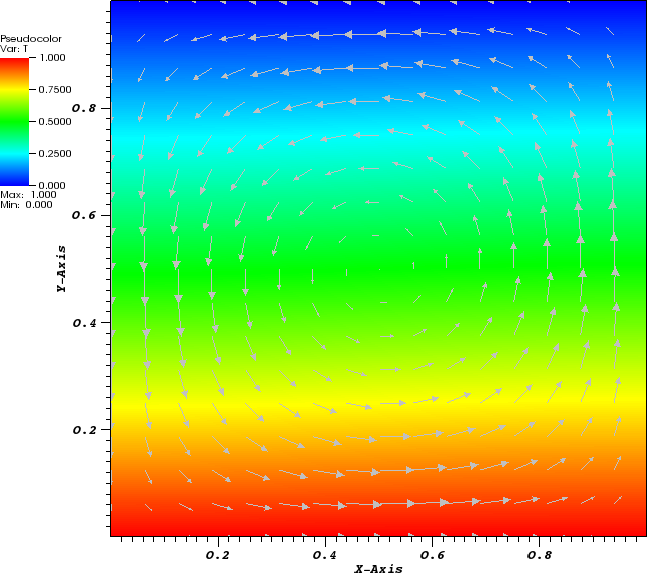
\includegraphics[width=0.4\textwidth]{cookbooks/convection-box/doc/visit0000.png}
\hfill
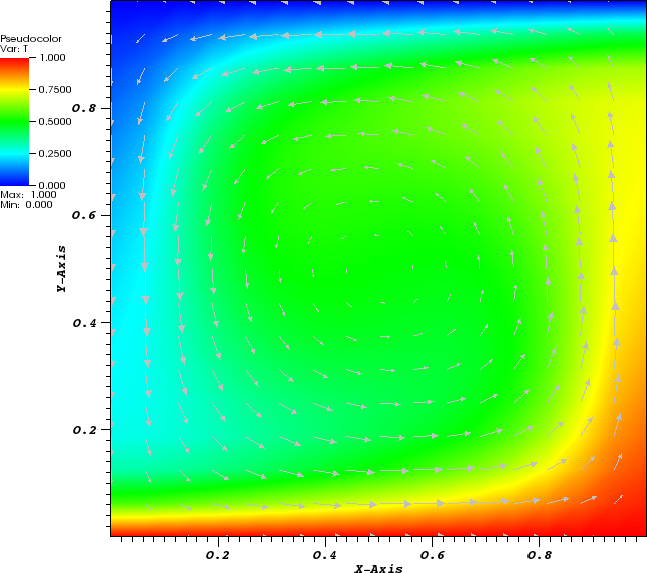
\includegraphics[width=0.4\textwidth]{cookbooks/convection-box/doc/visit0001.png}
\hfill
\phantom.
\caption{\it Convection in a box: Initial temperature and velocity field (left)
and final state (right).}
\label{fig:convection-box-fields}
\end{figure}

There are many other things we can learn from the output files generated by
\aspect{}, specifically from the statistics file that contains information
collected at every time step and that has been discussed in
Section~\ref{sec:viz-stat}. In particular, in our input file, we have selected
that we would like to compute velocity, temperature, and heat flux statistics.
These statistics, among others, are listed in the statistics file whose head
looks like this for the current input file:
\begin{lstlisting}[frame=single,language=prmfile]
# 1: Time step number
# 2: Time (seconds)
# 3: Time step size (seconds)
# 4: Number of mesh cells
# 5: Number of Stokes degrees of freedom
# 6: Number of temperature degrees of freedom
# 7: Iterations for temperature solver
# 8: Iterations for Stokes solver
# 9: Velocity iterations in Stokes preconditioner
# 10: Schur complement iterations in Stokes preconditioner
# 11: RMS velocity (m/s)
# 12: Max. velocity (m/s)
# 13: Minimal temperature (K)
# 14: Average temperature (K)
# 15: Maximal temperature (K)
# 16: Average nondimensional temperature (K)
# 17: Outward heat flux through boundary with indicator 0 ("left") (W)
# 18: Outward heat flux through boundary with indicator 1 ("right") (W)
# 19: Outward heat flux through boundary with indicator 2 ("bottom") (W)
# 20: Outward heat flux through boundary with indicator 3 ("top") (W)
# 21: Visualization file name
... lots of numbers arranged in columns ...
\end{lstlisting}

Fig.~\ref{fig:convection-box-stats} shows the results of visualizing the data
that can be found in columns 2 (the time) plotted against columns 11 and 12
(root mean square and maximal velocities). Plots of this kind can be generated with
\texttt{Gnuplot} by typing (see Section~\ref{sec:viz-stat} for a more thorough
discussion):
\begin{verbatim}
  plot "output-convection-box/statistics" using 2:11 with lines
\end{verbatim}
Fig.~\ref{fig:convection-box-stats} shows clearly that the simulation
enters a steady state after about $t\approx 0.1$ and then changes very little. This can also be observed using the
graphical output files from which we have generated
Fig.~\ref{fig:convection-box-fields}. One can look further into this data to
find that the flux through the top and bottom boundaries is not exactly the same
(up to the obvious difference in sign, given that at the bottom boundary heat
flows into the domain and at the top boundary out of it) at the beginning of the
simulation until the fluid has attained its equilibrium. However, after
$t\approx 0.2$, the fluxes differ by only $\num{5e-5}$, i.e., by less than
0.001\% of their magnitude.%
\footnote{This difference is far smaller than the numerical error in the heat
flux on the mesh this data is computed on.}
The flux we get at the last time step, 4.787, is less than 2\% away from the
value reported in \cite{BBC89} ($\approx$4.88) although we compute on a $16\times 16$ mesh and
the values reported by Blankenbach are extrapolated from meshes of size up to
$72\times 72$. This shows the accuracy that can be obtained using a higher order
finite element. Secondly, the fluxes through the left and right boundary are not
exactly zero but small. Of course, we have prescribed boundary conditions of the
form $\frac{\partial T}{\partial \mathbf n}=0$ along these boundaries, but this
is subject to discretization errors. It is easy to verify that the heat flux
through these two boundaries disappears as we refine the mesh further.

\begin{figure}
\phantom.
\hfill
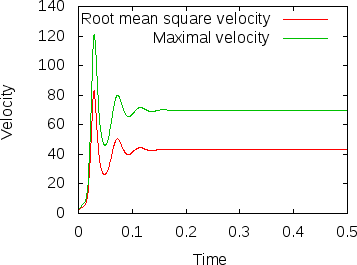
\includegraphics[width=0.4\textwidth]{cookbooks/convection-box/doc/velocity.png}
\hfill
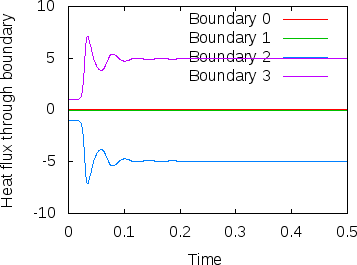
\includegraphics[width=0.4\textwidth]{cookbooks/convection-box/doc/heatflux.png}
\hfill
\phantom.
\caption{\it Convection in a box: Root mean square and maximal velocity as a
function of simulation time (left). Heat flux through the four boundaries of
the box (right).}
\label{fig:convection-box-stats}
\end{figure}


Furthermore, \aspect{} automatically also collects statistics about many of its
internal workings. Fig.~\ref{fig:convection-box-iterations} shows the number of
iterations required to solve the Stokes and temperature linear systems in each
time step. It is easy to see that these are more difficult to solve in the
beginning when the solution still changes significant from time step to time
step. However, after some time, the solution remains mostly the same and solvers
then only need 9 or 10 iterations for the temperature equation and 4 or 5
iterations for the Stokes equations because the starting guess for the linear
solver -- the previous time step's solution -- is already pretty good. If you
look at any of the more complex cookbooks, you will find that one needs many
more iterations to solve these equations.

\begin{figure}
\phantom.
\hfill
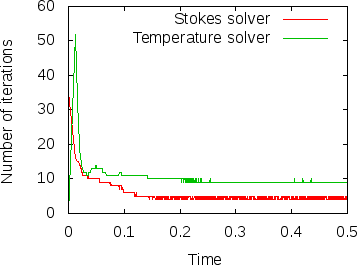
\includegraphics[width=0.4\textwidth]{cookbooks/convection-box/doc/iterations.png}
\hfill
\phantom.
\caption{\it Convection in a box: Number of linear iterations required to solve
the Stokes and temperature equations in each time step.}
\label{fig:convection-box-iterations}
\end{figure}

\note{If you want to run a version of this cookbook that uses Earth-like rather than nondimensional parameters, and that includes particles that visualize the flow field, see Section~\ref{sec:cookbooks-running-a-model}.}


\paragraph{Play time 1: Different Rayleigh numbers.} After showing you results
for the input file as it can be found in \url{cookbooks/convection-box.prm}, let us
end this section with a few ideas on how to play with it and what to explore.
The first direction one could take this example is certainly to consider
different Rayleigh numbers. As mentioned above, for the value $Ra=10^4$ for
which the results above have been produced, one gets a stable convection
pattern. On the other hand, for values $Ra<Ra_c\approx 780$, any movement of
the fluid dies down exponentially and we end up with a situation where the fluid
doesn't move and heat is transported from the bottom to the top only through
heat conduction. This can be explained by considering that the Rayleigh number
in a box is defined as $Ra=\frac{\rho_0 g\alpha\Delta T h^3}{\eta k}$. A small
Rayleigh number below $Ra_c$ means that the buoyancy forces 
caused by temperature variations 
-- $\rho_0 \alpha \Delta T$ -- are not strong enough to overcome friction forces within the fluid, that is, the viscosity is too high.

On the other hand, if the Rayleigh number is large (i.e., the viscosity is
small or the buoyancy large) then the fluid develops an unsteady convection
period. As we consider fluids with larger and larger $Ra$, this pattern goes
through a sequence of period-doubling events until flow finally becomes chaotic.
The structures of the flow pattern also become smaller and smaller.

\begin{figure}
\phantom.
\hfill
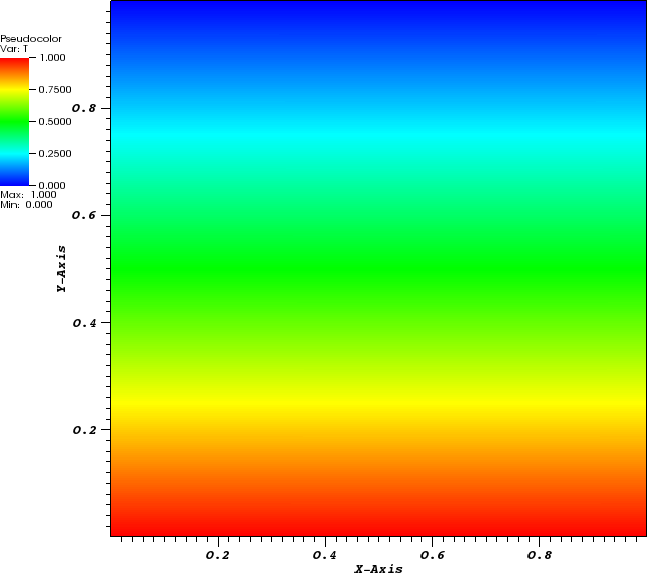
\includegraphics[width=0.4\textwidth]{cookbooks/convection-box/doc/ra_1e2_visit0000.png}
\hfill
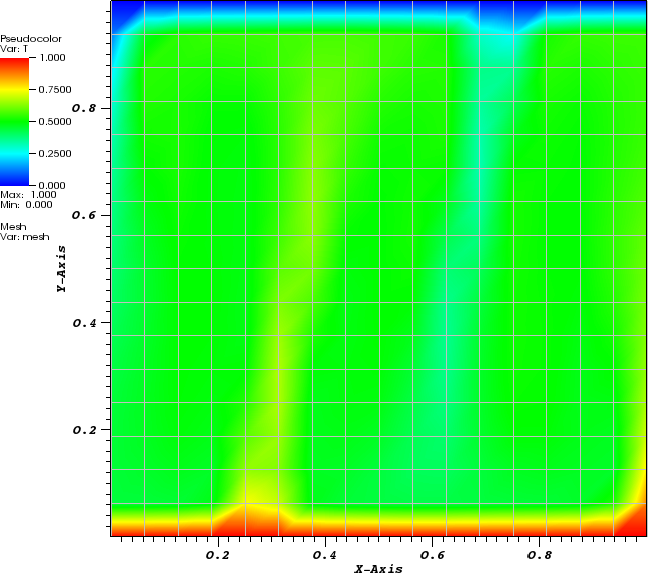
\includegraphics[width=0.4\textwidth]{cookbooks/convection-box/doc/ra_1e6_visit0001.png}
\hfill
\phantom.
\caption{\it Convection in a box: Temperature fields at the end of a
simulation for $Ra=10^2$ where thermal diffusion dominates (left) and $Ra=10^6$
where convective heat transport dominates (right).
The mesh on the right is clearly too coarse to resolve the structure of the solution.}
\label{fig:convection-box-fields-different-Ra}
\end{figure}

\begin{figure}
\phantom.
\hfill
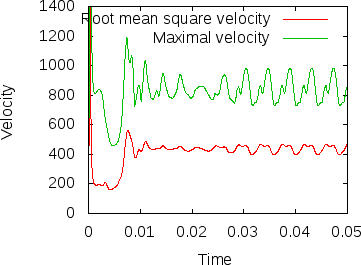
\includegraphics[width=0.4\textwidth]{cookbooks/convection-box/doc/ra_1e6_velocity.png}
\hfill
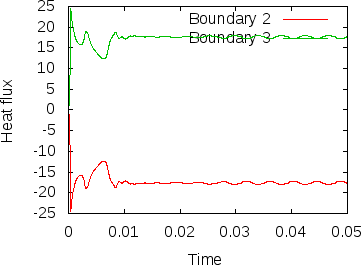
\includegraphics[width=0.4\textwidth]{cookbooks/convection-box/doc/ra_1e6_heatflux.png}
\hfill
\phantom.
\caption{\it Convection in a box: Velocities (left) and heat flux across the
top and bottom boundaries (right) as a function of time at $Ra=10^6$.}
\label{fig:convection-box-stats-different-Ra}
\end{figure}

We illustrate these situations in
Figs.~\ref{fig:convection-box-fields-different-Ra} and
\ref{fig:convection-box-stats-different-Ra}. The first shows the temperature
field at the end of a simulation for $Ra=10^2$ (below $Ra_c$) and at $Ra=10^6$.
Obviously, for the right picture, the mesh is not fine enough to accurately
resolve the features of the flow field and we would have to refine it more. The
second of the figures shows the velocity and heatflux statistics for the
computation with $Ra=10^6$; it is obvious here that the flow no longer settles
into a steady state but has a periodic behavior. This can also be seen by
looking at movies of the solution.

To generate these results, remember that we have chosen 
$g=Ra$ in our input file. In other words, changing the input file to
contain the parameter setting
%
\lstinputlisting[language=prmfile]{cookbooks/convection-box/doc/gravity.part.prm.out}
%
will achieve the desired effect of computing with $Ra=10^6$.


\paragraph{Play time 2: Thinking about finer meshes.}
In our computations for $Ra=10^4$ we used a $16\times 16$ mesh and obtained a
value for the heat flux that differed from the generally accepted value from
Blankenbach \textit{et al.} \cite{BBC89} by less than 2\%. However, it may be
interesting to think about computing even more accurately. This is easily done
by using a finer mesh, for example. In the parameter file above, we have chosen
the mesh setting as follows:
%
\lstinputlisting[language=prmfile]{cookbooks/convection-box/doc/refine.part.prm.out}
%
We start out with a box geometry consisting of a single cell that is refined
four times. Each time we split each cell into its 4 children, obtaining the
$16\times 16$ mesh already mentioned. The other settings indicate that we do not
want to refine the mesh adaptively at all in the first time step, and a setting
of zero for the last parameter means that we also never want to adapt the mesh
again at a later time. Let us stick with the never-changing, globally refined
mesh for now (we will come back to adaptive mesh refinement again at a later
time) and only vary the initial global refinement. In particular, we could
choose the parameter \texttt{Initial global refinement} to be 5, 6, or even
larger. This will get us closer to the exact solution albeit at the expense of a
significantly increased computational time.

A better strategy is to realize that for $Ra=10^4$, the flow enters a steady
state after settling in during the first part of the simulation (see, for
example, the graphs in Fig.~\ref{fig:convection-box-stats}). Since we are not
particularly interested in this initial transient process, there is really no
reason to spend CPU time using a fine mesh and correspondingly small time
steps during this part of the simulation (remember that each refinement results
in four times as many cells in 2d and a time step half as long, making reaching
a particular time at least 8 times as expensive, assuming that all solvers in
\aspect{} scale perfectly with the number of cells). Rather, we can use a
parameter in the \aspect{} input file that let's us increase the mesh resolution
at later times. To this end, let us use the following snippet for the input
file:
\lstinputlisting[language=prmfile]{cookbooks/convection-box/doc/refine2.part.prm.out}

What this does is the following: We start with an $8\times 8$ mesh (3 times
globally refined) but then at times $t=0.2,0.3$ and $0.4$ we refine the mesh
using the default refinement indicator (which one this is is not important
because of the next statement). Each time, we refine, we refine a fraction 1.0
of the cells, i.e., \textit{all} cells and we coarsen a fraction of 0.0 of the
cells, i.e. no cells at all. In effect, at these additional refinement times, we
do another global refinement, bringing us to refinement levels 4, 5 and finally
6.

\begin{figure}
\phantom.
\hfill
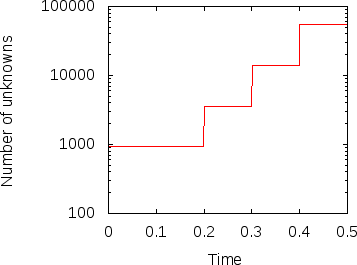
\includegraphics[width=0.4\textwidth]{cookbooks/convection-box/doc/steps_unknowns.png}
\hfill
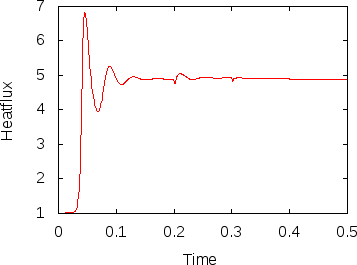
\includegraphics[width=0.4\textwidth]{cookbooks/convection-box/doc/steps_heatflux.png}
\hfill
\phantom.
\caption{\it Convection in a box: Refinement in stages. Total number
of unknowns in each time step, including all velocity, pressure and
temperature unknowns (left) and heat flux across the top boundary (right).}
\label{fig:convection-box-stats-steps}
\end{figure}


Fig.~\ref{fig:convection-box-stats-steps} shows the results. In the left panel,
we see how the number of unknowns grows over time (note the logscale for the
$y$-axis). The right panel displays the heat flux. The jumps in the number of
cells is clearly visible in this picture as well. This may be surprising at
first but remember that the mesh is clearly too coarse in the beginning to
really resolve the flow and so we should expect that the solution changes
significantly if the mesh is refined. This effect becomes smaller with every
additional refinement and is barely visible at the last time this happens,
indicating that the mesh before this refinement step may already have been fine
enough to resolve the majority of the dynamics.

In any case, we can compare the heat fluxes we obtain at the end of these
computations: With a globally four times refined mesh, we get a value of 4.787
(an error of approximately 2\% against the accepted value from Blankenbach,
$4.884409\pm 0.00001$). With a globally five times refined mesh we get 4.879, 
and with a globally six times refined mesh we get 4.89 (an error of almost 0.1\%).
With the mesh generated using the procedure above we also get
4.89 with the digits printed on the screen%
\footnote{The statistics file gives this
value to more digits: 4.89008498. However, these are clearly more digits than
the result is accurate.}
(also corresponding to an error of almost 0.1\%). In other words, our
simple procedure of refining the mesh during the simulation run yields the same 
accuracy as using the mesh that is globally refined in the beginning of the 
simulation, while needing a much lower compute time.  


\paragraph{Play time 3: Changing the finite element in use.}
Another way to increase the accuracy of a finite element computation is to use a
higher polynomial degree for the finite element shape functions. By default,
\aspect{} uses quadratic shape functions for the velocity and the temperature
and linear ones for the pressure. However, this can be changed with a single
number in the input file.

Before doing so, let us consider some aspects of such a change. First, looking
at the pictures of the solution in Fig.~\ref{fig:convection-box-fields}, one
could surmise that the quadratic elements should be able to resolve the velocity
field reasonably well given that it is rather smooth. On the other hand, the
temperature field has a boundary layer at the top and bottom. One could
conjecture that the temperature polynomial degree is therefore the limiting
factor and not the polynomial degree for the flow variables. We will test this
conjecture below. Secondly, given the nature of the equations, increasing the
polynomial degree of the flow variables increases the cost to solve these
equations by a factor of $\frac{22}{9}$ in 2d (you can get this factor by
counting the number of degrees of freedom uniquely associated with each cell) but leaves
the time step size and the cost of solving the temperature system unchanged. On
the other hand, increasing the polynomial degree of the temperature variable
from 2 to 3 requires $\frac 94$ times as many degrees of freedom for the
temperature and also requires us to reduce the size of the time step by a factor
of $\frac 23$. Because solving the temperature system is not a dominant factor
in each time step (see the timing results shown at the end of the screen output
above), the reduction in time step is the only important factor. Overall,
increasing the polynomial degree of the temperature variable turns out to be the
cheaper of the two options.

Following these considerations, let us add the following section to the
parameter file:
\lstinputlisting[language=prmfile]{cookbooks/convection-box/doc/disc.part.prm.out}

This leaves the velocity and pressure shape functions at quadratic and linear
polynomial degree but increases the polynomial degree of the temperature from
quadratic to cubic. Using the original, four times globally refined mesh, we
then get the following output:
\begin{lstlisting}[frame=single,language=ksh]
Number of active cells: 256 (on 5 levels)
Number of degrees of freedom: 4,868 (2,178+289+2,401)

*** Timestep 0:  t=0 seconds
   Solving temperature system... 0 iterations.
   Rebuilding Stokes preconditioner...
   Solving Stokes system... 30+0 iterations.

[... ...]

*** Timestep 1621:  t=0.5 seconds
   Solving temperature system... 0 iterations.
   Solving Stokes system... 1+0 iterations.

   Postprocessing:
     RMS, max velocity:                  42.9 m/s, 69.5 m/s
     Temperature min/avg/max:            0 K, 0.5 K, 1 K
     Heat fluxes through boundary parts: -0.004602 W, 0.004602 W, -4.849 W, 4.849 W

Termination requested by criterion: end time


+---------------------------------------------+------------+------------+
| Total wallclock time elapsed since start    |      53.6s |            |
|                                             |            |            |
| Section                         | no. calls |  wall time | % of total |
+---------------------------------+-----------+------------+------------+
| Assemble Stokes system          |      1622 |      4.04s |       7.5% |
| Assemble temperature system     |      1622 |      24.4s |        46% |
| Build Stokes preconditioner     |         1 |    0.0121s |         0% |
| Build temperature preconditioner|      1622 |      8.05s |        15% |
| Solve Stokes system             |      1622 |      8.92s |        17% |
| Solve temperature system        |      1622 |      1.67s |       3.1% |
| Initialization                  |         1 |    0.0327s |         0% |
| Postprocessing                  |      1622 |      4.27s |         8% |
| Setup dof systems               |         1 |   0.00418s |         0% |
| Setup initial conditions        |         1 |   0.00236s |         0% |
+---------------------------------+-----------+------------+------------+

\end{lstlisting}

The heat flux through the top and bottom boundaries is now computed as 4.878.
Using the five times globally refined mesh, it is 4.8837 (an error of 0.015\%). 
This is 6 times more accurate than the 
once more globally refined mesh with the original quadratic elements, at a cost
significantly smaller. Furthermore, we can of course combine this with the mesh
that is gradually refined as simulation time progresses, and we then get a heat
flux that is equal to 4.884446, also only 0.01\% away from the accepted value!

As a final remark, to test our hypothesis that it was indeed the temperature
polynomial degree that was the limiting factor, we can increase the Stokes
polynomial degree to 3 while leaving the temperature polynomial degree at 2. A
quick computation shows that in that case we get a heat flux of 4.747 -- almost 
the same value as we got initially with the lower order Stokes element. In other
words, at least for this testcase, it really was the temperature variable that
limits the accuracy.


% cookbooks/convection_box_3d
\subsubsection{Convection in a 3d box}
\label{sec:cookbooks-simple-box-3d}

The world is not two-dimensional. While the previous section introduced a number
of the knobs one can play with with \aspect{}, things only really become
interesting once one goes to 3d. The setup from the previous section is easily
adjusted to this and in the following, let us walk through some of the changes
we have to consider when going from 2d to 3d. The full input file that
contains these modifications and that was used for the simulations we will show
subsequently can be found at \url{cookbooks/convection\_box\_3d.prm}.

The first set of changes has to do with the geometry: it is three-dimensional,
and we will have to address the fact that a box in 3d has 6 sides, not the 4 we
had previously. The documentation of the ``box'' geometry
(see Section~\ref{parameters:Geometry_20model}) states that these sides are
numbered as follows: ``\textit{in 3d, boundary indicators 0 through 5 indicate
left, right, front, back, bottom and top boundaries}.'' Recalling that we want
tangential flow all around and want to fix the temperature to known values at
the bottom and top, the following will make sense:
\lstinputlisting[language=prmfile]{start.part.prm.out}


The next step is to describe the initial conditions. As before, we will use an
unstably layered medium but the perturbation now needs to be both in $x$- and
$y$-direction
\lstinputlisting[language=prmfile]{initial.part.prm.out}

The third issue we need to address is that we can likely not afford a mesh as
fine as in 2d. We choose a mesh that is refined 3 times globally at the
beginning, then 3 times adaptively, and is then adapted every 15 time steps. We
also allow one additional mesh refinement in the first time step following
$t=0.003$ once the initial instability has given way to a more stable pattern:
\lstinputlisting[language=prmfile]{amr.part.prm.out}

Finally, as we have seen in the previous section, a computation with $Ra=10^4$
does not lead to a simulation that is exactly exciting. Let us choose $Ra=10^6$
instead (the mesh chosen above with up to 7 refinement levels after some time
is fine enough to resolve this). We can achieve this in the same way as in the
previous section by choosing $\alpha=10^{-10}$ and setting
\lstinputlisting[language=prmfile]{gravity.part.prm.out}
This has some interesting implications. First, a higher Rayleigh number makes
time scales correspondingly smaller; where we generated graphical output only
once every 0.01 time units before, we now need to choose the corresponding
increment smaller by a factor of 100:
\lstinputlisting[language=prmfile]{postprocess.part.prm.out}
Secondly, a simulation like this -- in 3d, with a significant number of cells,
and for a significant number of time steps -- will likely take a good amount of
time. The computations for which we show results below was run using 64
processors by running it using the command
{\tt{mpirun -n 64 ./aspect convection\_box\_3d.prm}}. If the machine should crash
during such a run, a significant amount of compute time would be lost if we had
to run everything from the start. However, we can avoid this by periodically
checkpointing the state of the computation:
\lstinputlisting[language=prmfile]{checkpoint.part.prm.out}
If the computation does crash (or if a computation runs out of the time limit
imposed by a scheduling system), then it can be restarted from such
checkpointing files (see the parameter {\tt Resume computation}
in Section~\ref{parameters:global}).
\index[prmindex]{Resume computation}
\index[prmindexfull]{Resume computation}

Running with this input file requires a bit of patience%
\footnote{For computations of this size, one should test a few time steps in
  debug mode but then, of course, switch to running the actual computation in
  optimized mode -- see Section~\ref{sec:debug-mode}.}
since the number of
degrees of freedom is just so large: it starts with a bit over 330,000\ldots
\begin{lstlisting}[frame=single,language=ksh]
Running with 64 MPI tasks.
Number of active cells: 512 (on 4 levels)
Number of degrees of freedom: 20,381 (14,739+729+4,913)

*** Timestep 0:  t=0 seconds
   Solving temperature system... 0 iterations.
   Rebuilding Stokes preconditioner...
   Solving Stokes system... 18 iterations.

Number of active cells: 1,576 (on 5 levels)
Number of degrees of freedom: 63,391 (45,909+2,179+15,303)

*** Timestep 0:  t=0 seconds
   Solving temperature system... 0 iterations.
   Rebuilding Stokes preconditioner...
   Solving Stokes system... 19 iterations.

Number of active cells: 3,249 (on 5 levels)
Number of degrees of freedom: 122,066 (88,500+4,066+29,500)

*** Timestep 0:  t=0 seconds
   Solving temperature system... 0 iterations.
   Rebuilding Stokes preconditioner...
   Solving Stokes system... 20 iterations.

Number of active cells: 8,968 (on 5 levels)
Number of degrees of freedom: 331,696 (240,624+10,864+80,208)

*** Timestep 0:  t=0 seconds
   Solving temperature system... 0 iterations.
   Rebuilding Stokes preconditioner...
   Solving Stokes system... 21 iterations.
[...]
\end{lstlisting}
\ldots{}but then increases quickly to around 2 million as the solution develops
some structure and, after time $t=0.003$ where we allow for an additional
refinement, increases to over 10 million where it then hovers between 8 and 14
million with a maximum of 15,147,534. Clearly, even on a reasonably quick
machine, this will take some time: running this on a machine bought in 2011,
doing the 10,000 time steps to get to $t=0.0219$ takes approximately 484,000
seconds (about five and a half days).

The structure or the solution is easiest to grasp by looking at isosurfaces of
the temperature. This is shown in Fig.~\ref{fig:box-3d-solution} and you can
find a movie of the motion that ensues from the heating at the bottom at
\url{http://www.youtube.com/watch?v=_bKqU_P4j48}. The simulation uses adaptively
changing meshes that are fine in rising plumes and sinking blobs and are coarse
where nothing much happens. This is most easily seen in the movie at
\url{http://www.youtube.com/watch?v=CzCKYyR-cmg}. Fig.~\ref{fig:box-3d-mesh}
shows some of these meshes, though still pictures do not do the evolving nature
of the mesh much justice. The effect of increasing the Rayleigh number is
apparent when comparing the size of features with, for example, the picture at
the right of Fig.~\ref{fig:convection-box-fields}. In contrast to that picture,
the simulation is also clearly non-stationary.

\begin{figure}
  \centering
  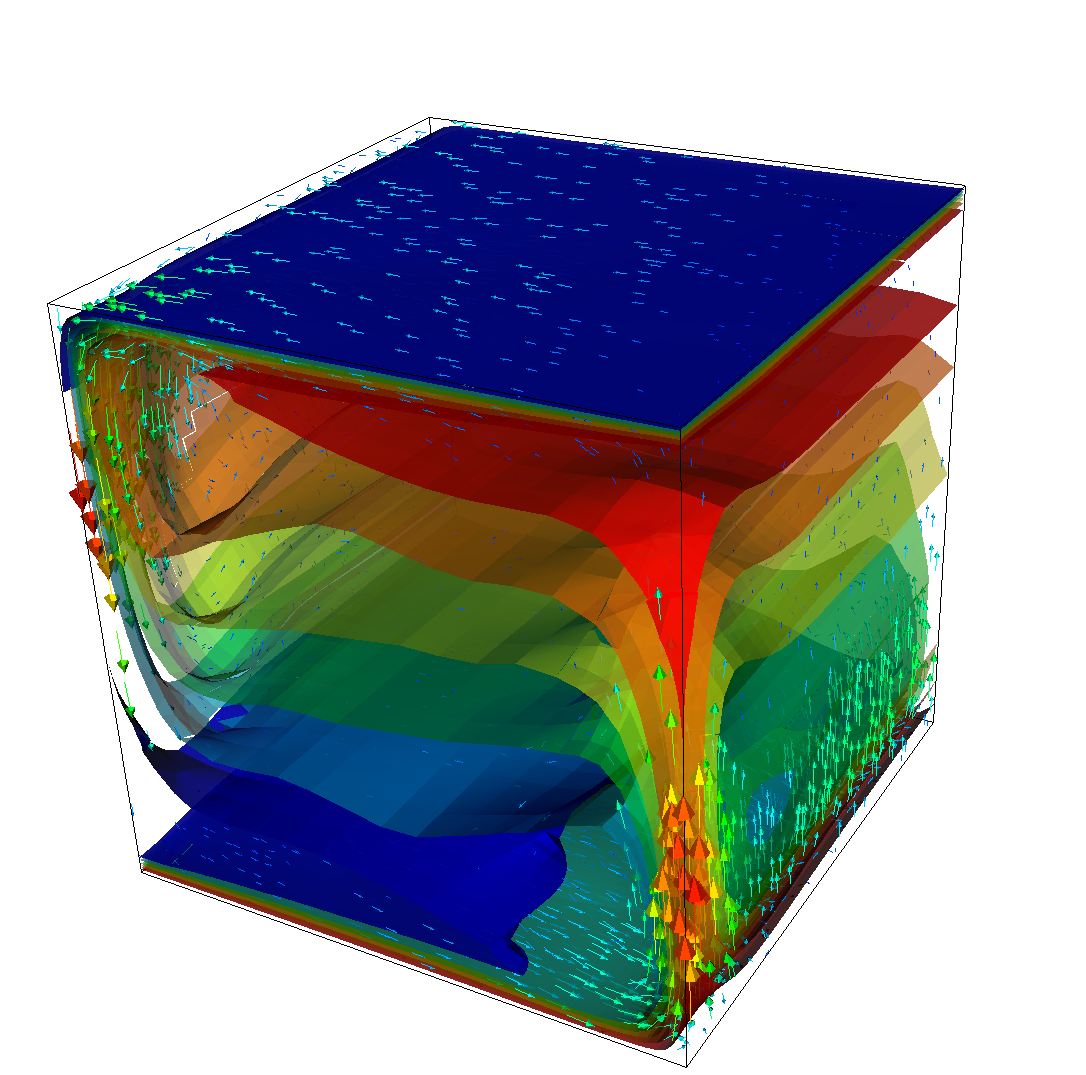
\includegraphics[width=0.3\textwidth]{movie0010.png}
  \hfill
  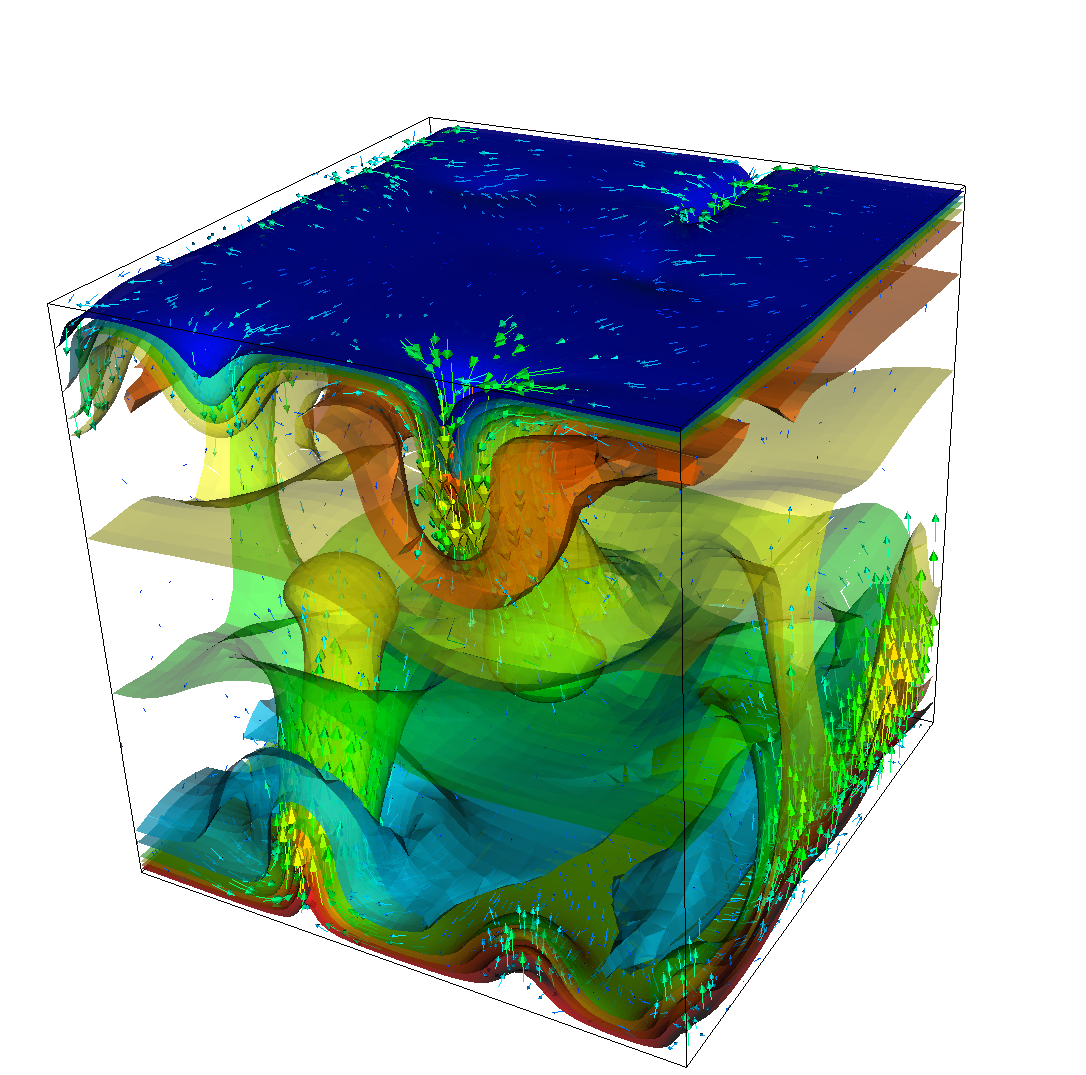
\includegraphics[width=0.3\textwidth]{movie0040.png}
  \hfill
  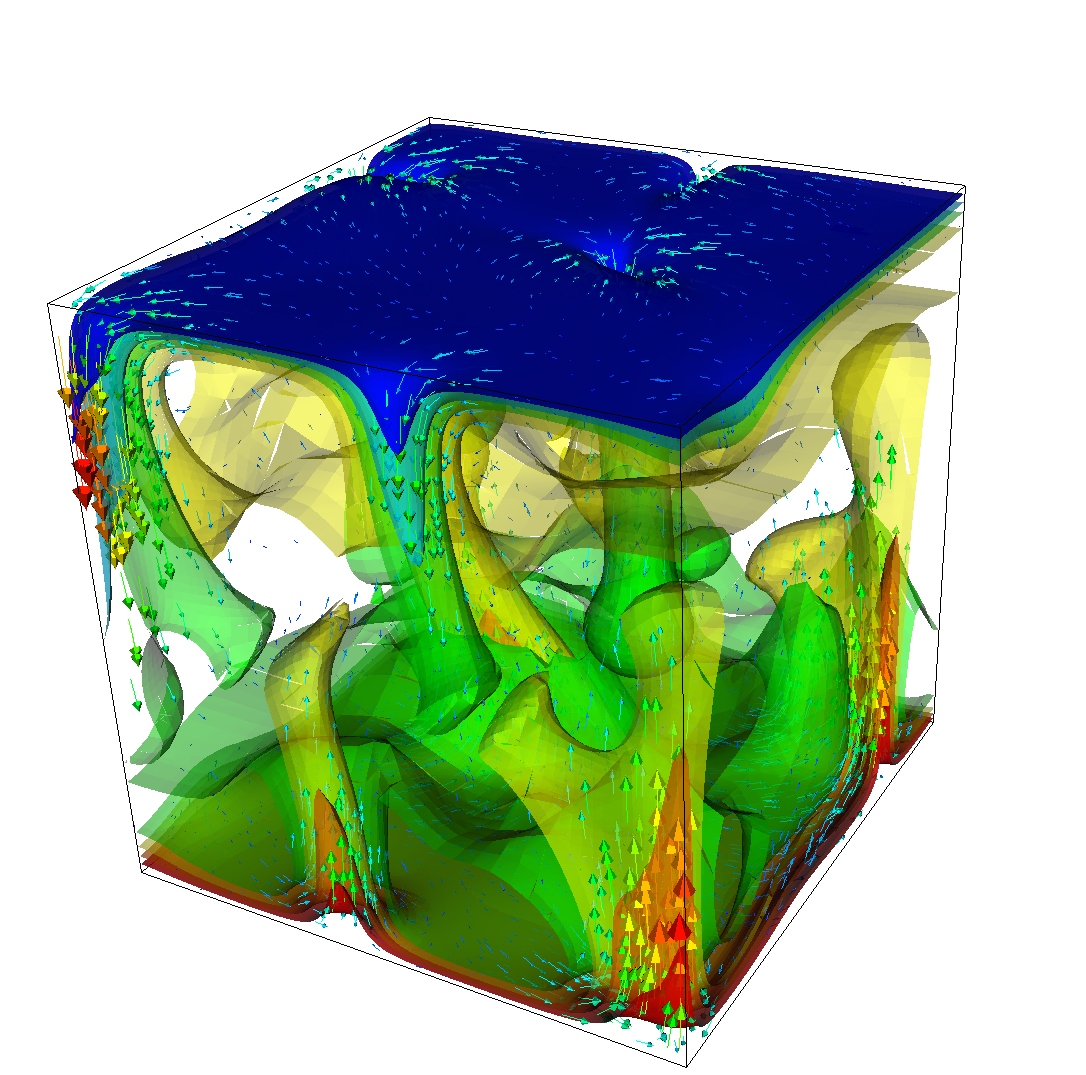
\includegraphics[width=0.3\textwidth]{movie0060.png}
  \\
  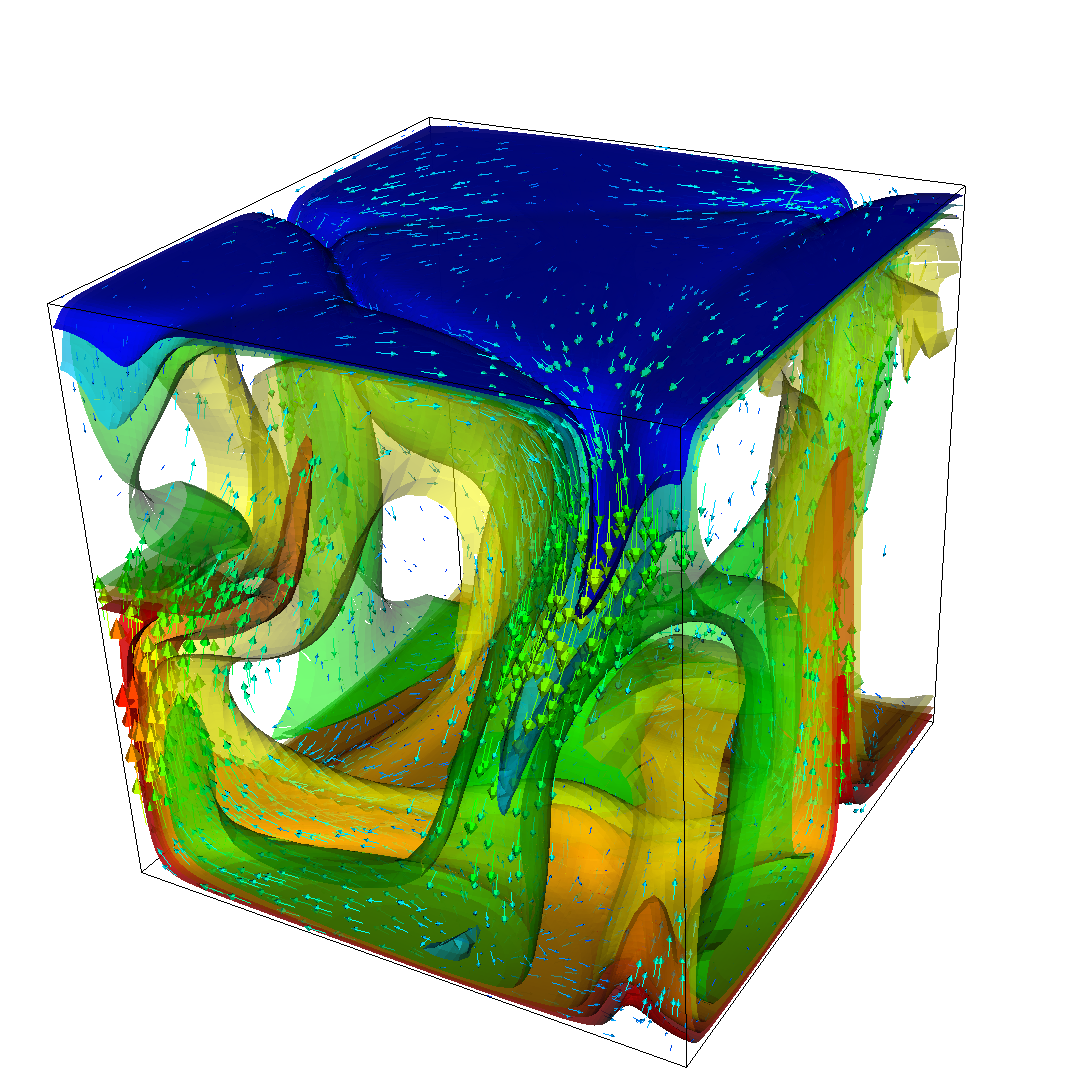
\includegraphics[width=0.3\textwidth]{movie0100.png}
  \hfill
  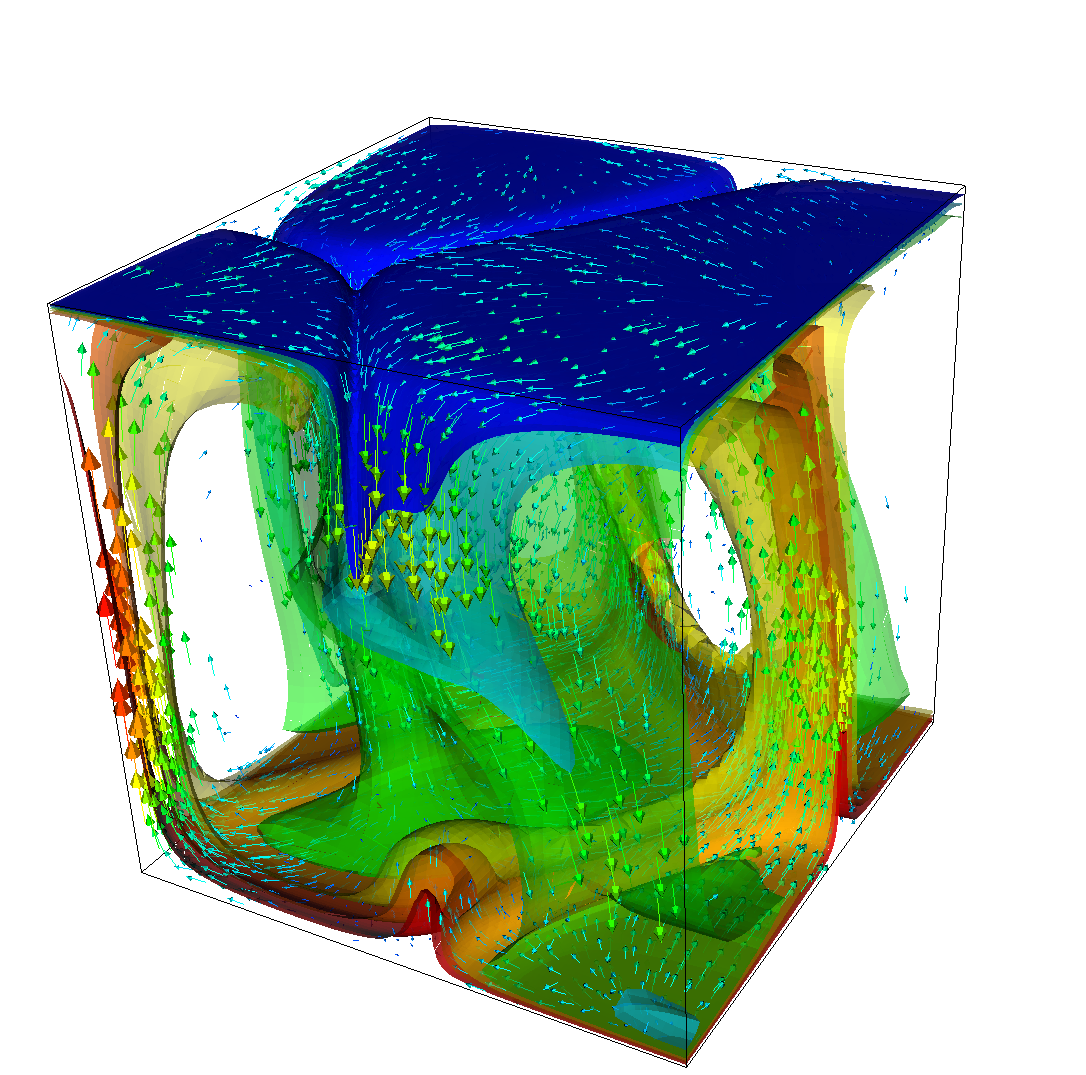
\includegraphics[width=0.3\textwidth]{movie0130.png}
  \hfill
  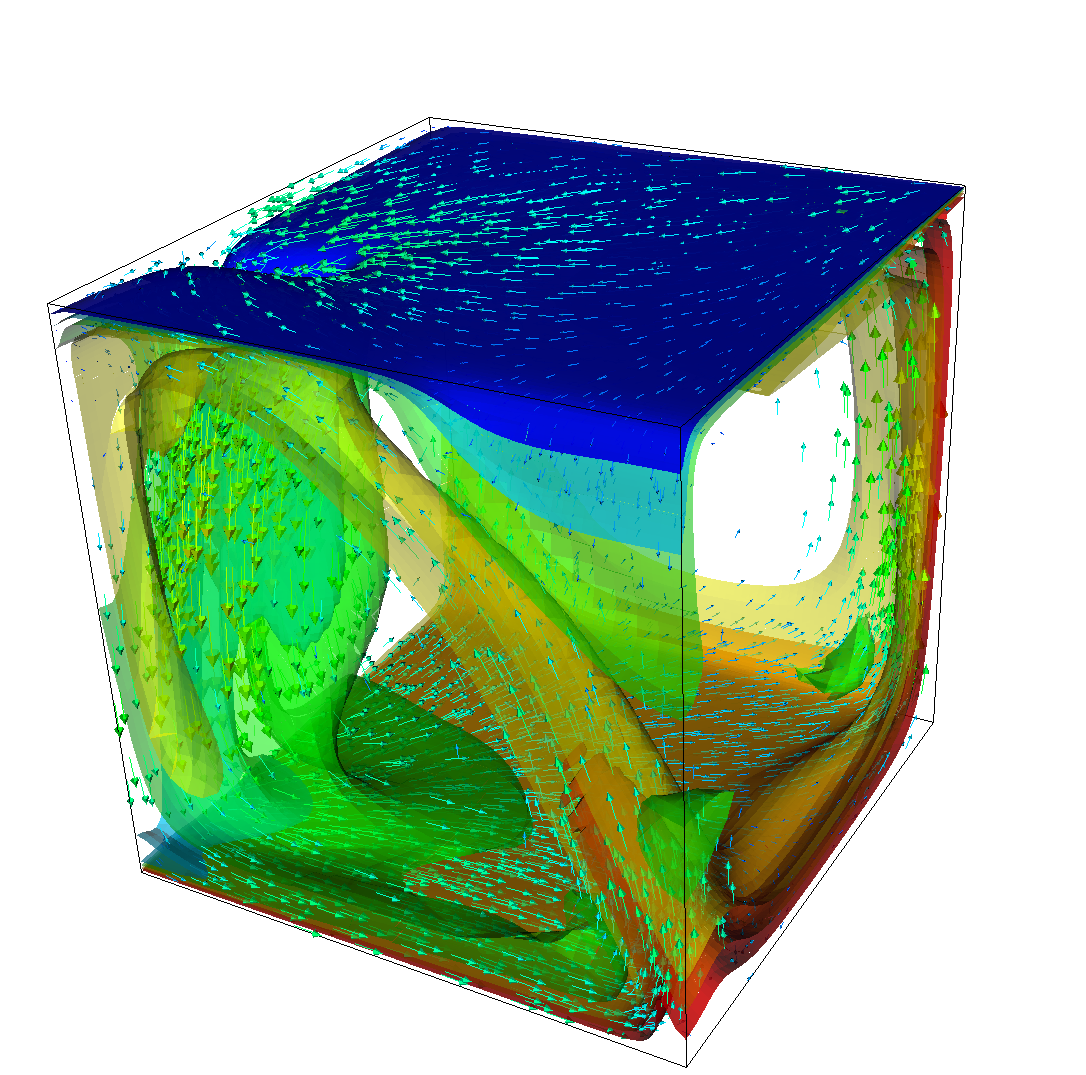
\includegraphics[width=0.3\textwidth]{movie0180.png}
  \caption{\it Convection in a 3d box: Temperature isocontours and some
  velocity vectors at the first time step after times $t=0.001, 0.004, 0.006$
  (top row, left to right) an $t=0.01, 0.013, 0.018$ (bottom row).}
  \label{fig:box-3d-solution}
\end{figure}


\begin{figure}
  \centering
  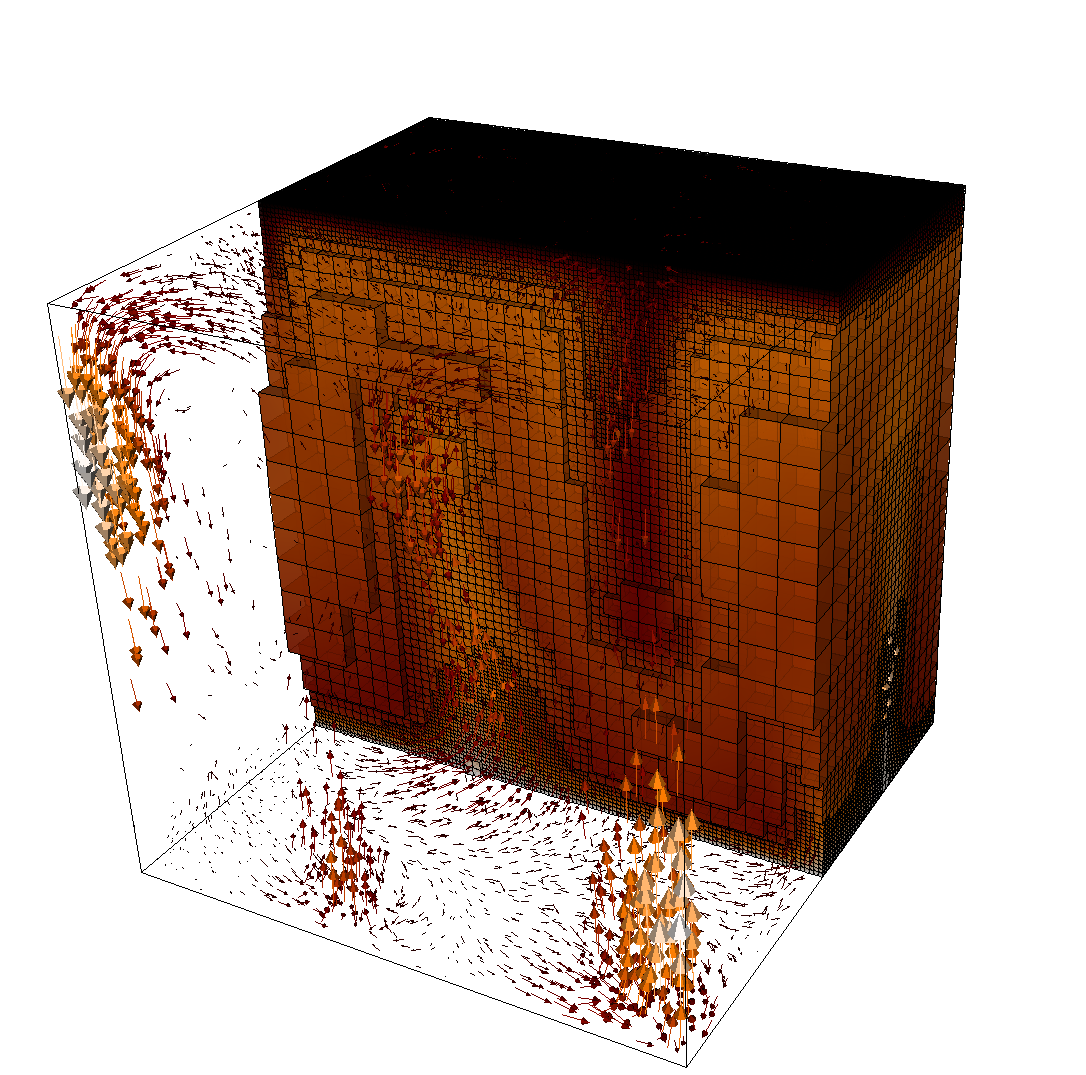
\includegraphics[width=0.3\textwidth]{mesh0060.png}
  \hfill
  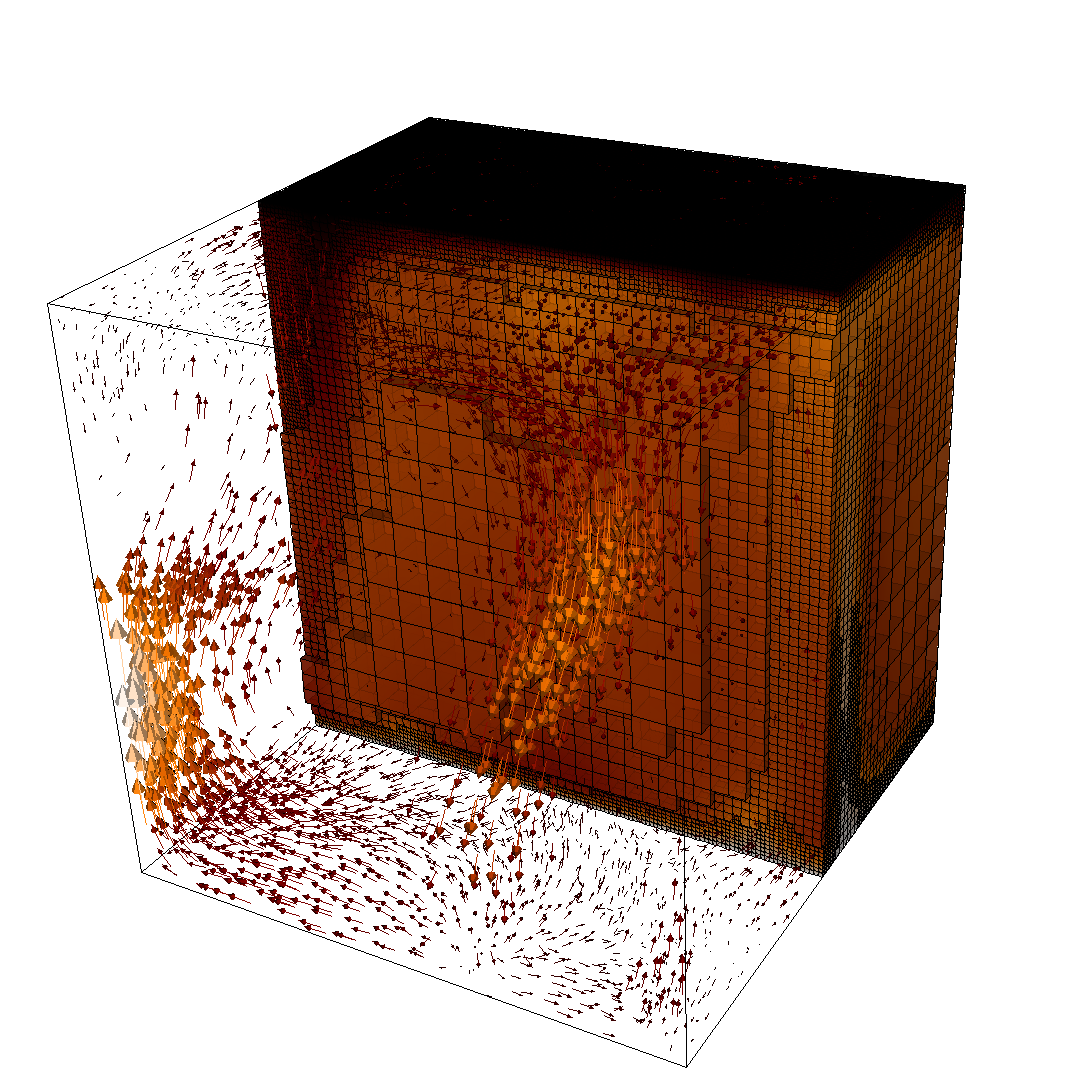
\includegraphics[width=0.3\textwidth]{mesh0100.png}
  \hfill
  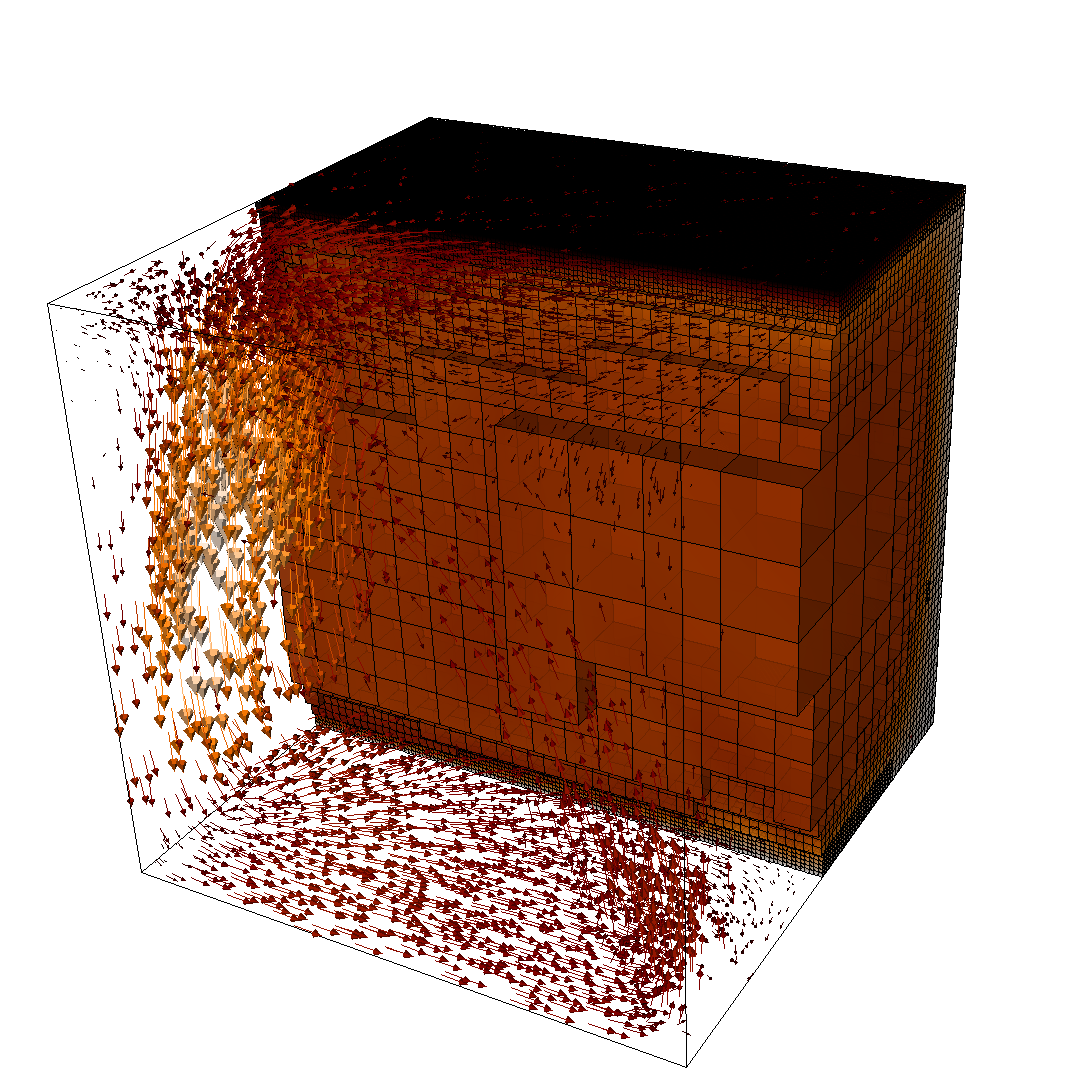
\includegraphics[width=0.3\textwidth]{mesh0180.png}
  \caption{\it Convection in a 3d box: Meshes and large-scale velocity field
  for the third, fourth and sixth of the snapshots shown in
  Fig.~\ref{fig:box-3d-solution}.}
  \label{fig:box-3d-mesh}
\end{figure}

As before, we could analyze all sorts of data from the statistics file but we
will leave this to those interested in specific data. Rather,
Fig.~\ref{fig:box-3d-heat-flux} only shows the upward heat flux through the
bottom and top boundaries of the domain as a function of time.%
\footnote{Note that the statistics file actually contains the \textit{outward}
heat flux for each of the six boundaries, which corresponds to the
\textit{negative} of upward flux for the bottom boundary. The figure therefore
shows the negative of the values available in the statistics file.}
The figure reinforces a pattern that can also be seen by watching the movie of
the temperature field referenced above, namely that the simulation can be
subdivided into three distinct phases. The first phase corresponds to the
initial overturning of the unstable layering of the temperature field and is
associated with a large spike in heat flux as well as large velocities (not
shown here). The second phase, until approximately $t=0.01$ corresponds to a
relative lull: some plumes rise up, but not very fast because the medium is now
stably layered but not fully mixed. This can be seen in the relatively low heat
fluxes, but also in the fact that there are almost horizontal temperature
isosurfaces in the second of the pictures in Fig.~\ref{fig:box-3d-solution}.
After that, the general structure of the temperature field is that the interior
of the domain is well mixed with a mostly constant average temperature and thin
thermal boundary layers at the top and bottom from which plumes rise and sink.
In this regime, the average heat flux is larger but also more variable depending
on the number of plumes currently active. Many other analyses would be possible
by using what is in the statistics file or by enabling additional
postprocessors.

\begin{figure}
  \centering
  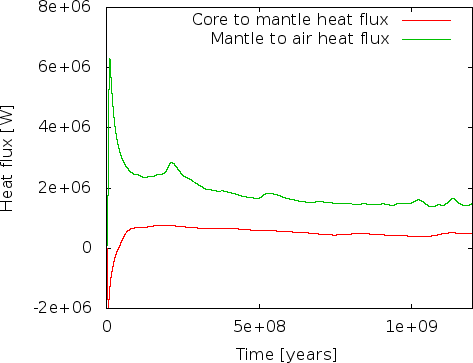
\includegraphics[width=0.6\textwidth]{heat-flux.png}
  \caption{\it Convection in a 3d box: Upward heat flux through the bottom and
  top boundaries as a function of time.}
  \label{fig:box-3d-heat-flux}
\end{figure}





% cookbooks/platelike-boundary
\subsubsection{Convection in a box with prescribed, variable velocity boundary conditions}
\label{sec:cookbooks-platelike}

A similarly simple setup to the ones considered in the previous subsections is
to equip the model we had with a different set of boundary conditions. There, we used slip boundary
conditions, i.e., the fluid can flow tangentially along the four sides of our
box but this tangential velocity is unspecified. On the other hand, in many
situations, one would like to actually prescribe the tangential flow velocity as
well. A typical application would be to use boundary conditions at the top that
describe experimentally determined velocities of plates. This cookbook shows a
simple version of something like this. To make it slightly more interesting, we
choose a $2\times 1$ domain in 2d.

Like for many other things, \aspect{} has a set of plugins for prescribed
velocity boundary values (see
Sections~\ref{parameters:Boundary_20velocity_20model} and
\ref{sec:prescribed-velocity-boundary-conditions}). These plugins allow one to
write sophisticated models for the boundary velocity on parts or all of the
boundary, but there is also one simple implementation that just takes a formula
for the components of the velocity.

To illustrate this, let us consider the \url{cookbooks/platelike-boundary/platelike-boundary.prm}
input file. It essentially extends the input file considered in the previous example.
The part of this file that we are particularly interested in in the current
context is the selection of the kind of velocity boundary conditions on the four
sides of the box geometry, which we do using a section like this:
\lstinputlisting[language=prmfile]{cookbooks/platelike-boundary/doc/boundary.part.prm.out}

We use tangential flow at boundaries named left, right and bottom.
Additionally, we specify a comma separated list (here with only a single
element) of pairs consisting of the name of a boundary and the name of a
prescribed velocity boundary model. Here, we use the \texttt{function} model on
the \texttt{top} boundary, which allows us to provide a function-like notation
for the components of the velocity vector at the boundary.

The second part we need is that we actually describe the function that sets the
velocity. We do this in the subsection \texttt{Function}. The first of these
parameters gives names to the components of the position vector (here, we are
in 2d and we use $x$ and $z$ as spatial variable names) and the time. We could
have left this entry at its default, \texttt{x,y,t}, but since we
often think in terms of ``depth'' as the vertical direction, let us use
\texttt{z} for the second coordinate.
In the second parameter we define symbolic constants that can be used
in the formula for the velocity that is specified in the last parameter. This
formula needs to have as many components as there are space dimensions,
separated by semicolons. As stated, this means that we prescribe the
(horizontal) $x$-velocity and set the vertical velocity to zero. The horizontal
component is here either $1$ or $-1$, depending on whether we are to the right
or the left of the point $1+\sin(\pi t/2)$ that is moving back and forth with
time once every four time units. The \texttt{if} statement understood by the
parser we use for these formulas has the syntax
\texttt{if(condition, value-if-true, value-if-false)}.

\note{While you can enter most any expression into the parser for these
velocity boundary conditions, not all make sense. In particular, if you use an
incompressible medium like we do here, then you need to make sure that either
the flow you prescribe is indeed tangential, or that at least the flow into and
out of the boundary this function applies to is balanced so that in sum the
amount of material in the domain stays constant.

It is in general not possible for \aspect{} to verify that a given input is
sensible. However, you will quickly find out if it isn't: The linear solver for
the Stokes equations will simply not converge. For example, if your function
expression in the input file above read \\
\hspace*{.25cm} \texttt{if(x>1+sin(0.5*pi*t), 1, -1); 1}\\
then at the time of writing this you would get the following error message: \\
\hspace*{.25cm}\texttt{*** Timestep 0:  t=0 seconds} \\
\hspace*{.25cm}\texttt{   Solving temperature system... 0 iterations.} \\
\hspace*{.25cm}\texttt{   Rebuilding Stokes preconditioner...} \\
\hspace*{.25cm}\texttt{   Solving Stokes system... } \\
\\
\hspace*{.25cm}\texttt{\ldots some timing output \ldots} \\
\\
\\
\hspace*{.25cm}\texttt{----------------------------------------------------} \\
\hspace*{.25cm}\texttt{Exception on processing: } \\
\hspace*{.25cm}\texttt{Iterative method reported convergence failure in step
9539 with residual 6.0552} \\
\hspace*{.25cm}\texttt{Aborting!} \\
\hspace*{.25cm}\texttt{----------------------------------------------------}

The reason is, of course, that there is no incompressible (divergence free) flow
field that allows for a constant vertical outflow component along the top
boundary without corresponding inflow anywhere else.}


The remainder of the setup is described in the following, complete input file:
\lstinputlisting[language=prmfile]{cookbooks/platelike-boundary/doc/platelike.prm.out}


This model description yields a setup with a Rayleigh number of 200 (taking
into account that the domain has size 2). It would, thus, be dominated by heat
conduction rather than convection if the prescribed velocity boundary conditions
did not provide a stirring action. Visualizing the results of this simulation%
\footnote{In fact, the pictures are generated using a twice more refined mesh
to provide adequate resolution. We keep the default setting of five
global refinements in the parameter file as documented above to keep compute
time reasonable when using the default settings.}
yields images like the ones shown in Fig.~\ref{fig:platelike}.

\begin{figure}
  \centering
  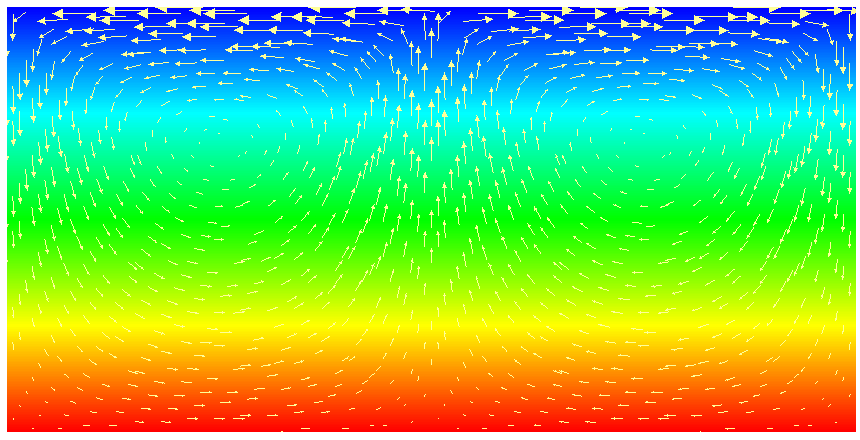
\includegraphics[width=0.3\textwidth]{cookbooks/platelike-boundary/doc/visit0000.png}
  \hfill
  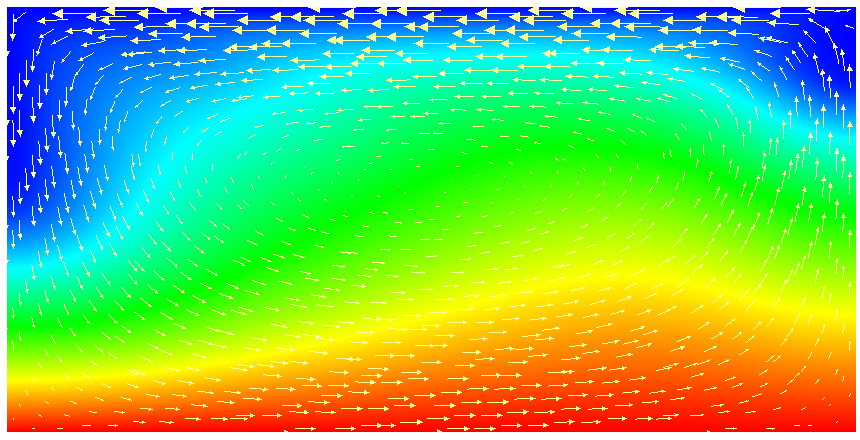
\includegraphics[width=0.3\textwidth]{cookbooks/platelike-boundary/doc/visit0001.png}
  \hfill
  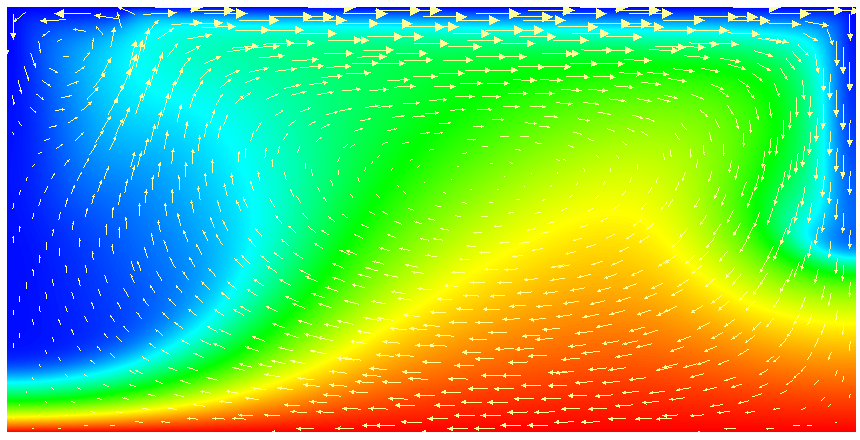
\includegraphics[width=0.3\textwidth]{cookbooks/platelike-boundary/doc/visit0003.png}
  \\
  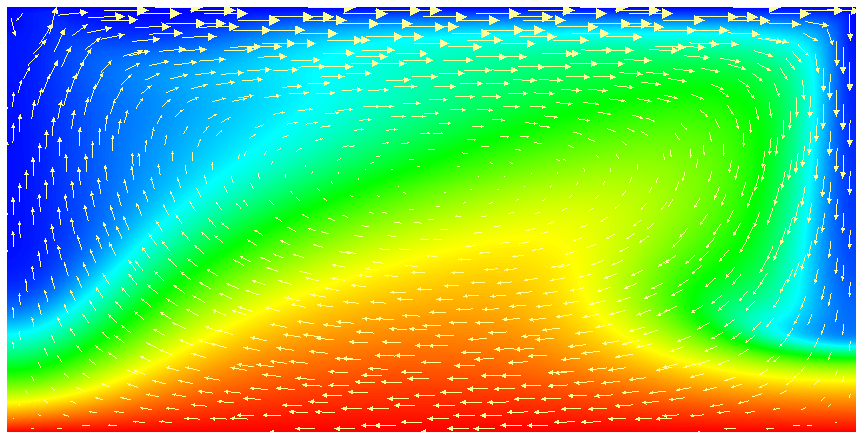
\includegraphics[width=0.3\textwidth]{cookbooks/platelike-boundary/doc/visit0004.png}
  \hfill
  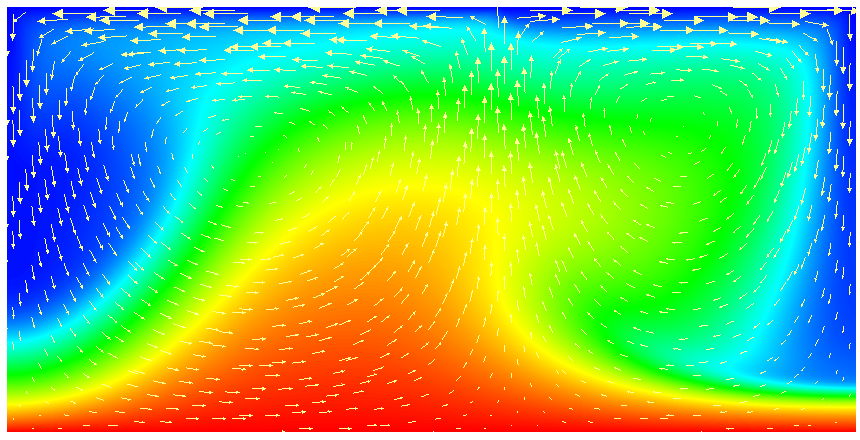
\includegraphics[width=0.3\textwidth]{cookbooks/platelike-boundary/doc/visit0005.png}
  \hfill
  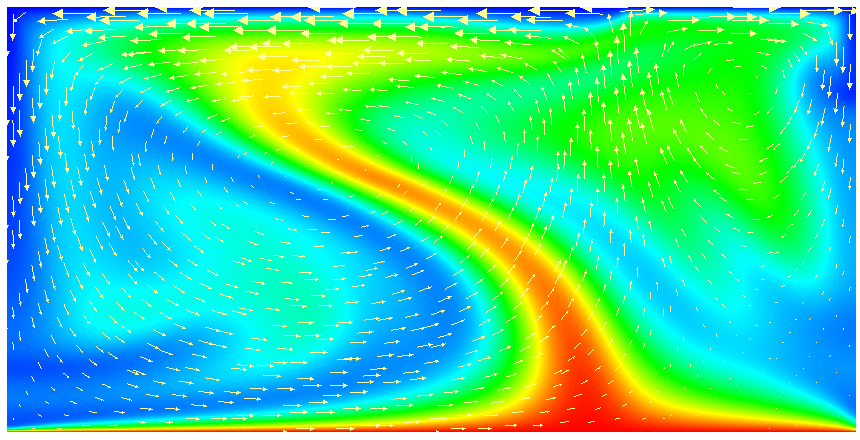
\includegraphics[width=0.3\textwidth]{cookbooks/platelike-boundary/doc/visit0006.png}
  \caption{\it Variable velocity boundary conditions: Temperature and velocity
  fields at the initial time (top left) and at various other points in time during the
  simulation.}
  \label{fig:platelike}
\end{figure}





\subsubsection{Using passive and active compositional fields}
\label{sec:cookbooks-composition}

One frequently wants to track where material goes, either because one simply
wants to see where stuff ends up (e.g., to determine if a particular model
yields mixing between the lower and upper mantle) or because the material model
in fact depends not only pressure, temperature and location but also on the
mass fractions of certain chemical or other species. We will refer to the first
case as \textit{passive} and the latter as \textit{active} to indicate the role
of the additional quantities whose distribution we want to track. We refer to
the whole process as \textit{compositional} since we consider quantities that
have the flavor of something that denotes the composition of the material at any
given point.

There are basically two ways to achieve this: one can advect a set of
particles (``tracers'') along with the velocity field, or one can advect along a
field. In the first case, where the closest particle came from indicates the
value of the concentration at any given position. In the latter case, the
concentration(s) at any given position is simply given by the value of the
field(s) at this location.

\aspect{} implements both strategies, at least to a certain degree. In this
cookbook, we will follow the route of advected fields.


% cookbooks/composition_active/

\paragraph{The passive case.}
We will consider the
exact same situation as in the previous section but we will ask where the
material that started in the bottom 20\% of the domain
ends up, as well as the material that started in the top 20\%. For the moment,
let us assume that there is no material between the materials at the bottom, the
top, and the middle. The way to describe this situation is to simply add the
following block of definitions to the parameter file (you can find the full
parameter file in \url{cookbooks/composition_passive/composition_passive.prm}:

\lstinputlisting[language=prmfile]{cookbooks/composition_passive/doc/passive.part.prm.out}

Running this simulation yields results such as the ones shown in
Fig.~\ref{fig:compositional-passive} where we show the values of the functions
$c_1(\mathbf x,t)$ and $c_2(\mathbf x,t)$ at various times in the simulation.
Because these fields were one only inside the lowermost and uppermost parts of
the domain, zero everywhere else, and because they have simply been advected
along with the flow field, the places where they are larger than one half
indicate where material has been transported to so far.%
\footnote{Of course, this interpretation suggests that we could have achieved
the same goal by encoding everything into a single function -- that would, for
example, have had initial values one, zero and minus one in the three parts of
the domain we are interested in.}

\begin{figure}
  \centering
  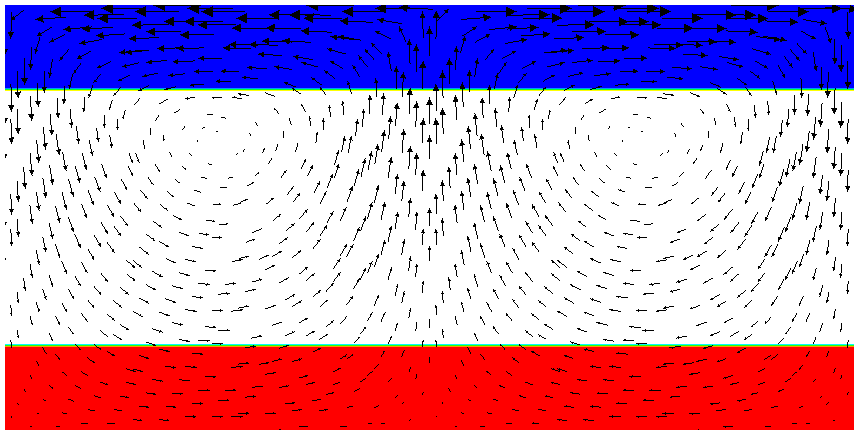
\includegraphics[width=0.3\textwidth]{cookbooks/composition_passive/doc/visit0007.png}
  \hfill
  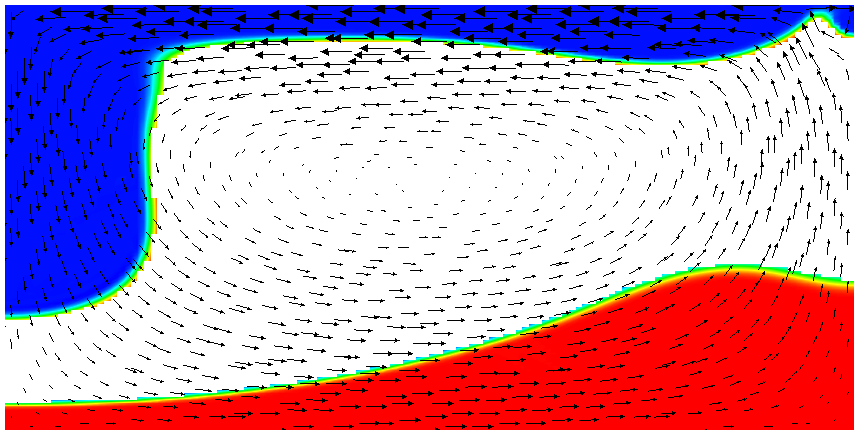
\includegraphics[width=0.3\textwidth]{cookbooks/composition_passive/doc/visit0008.png}
  \hfill
  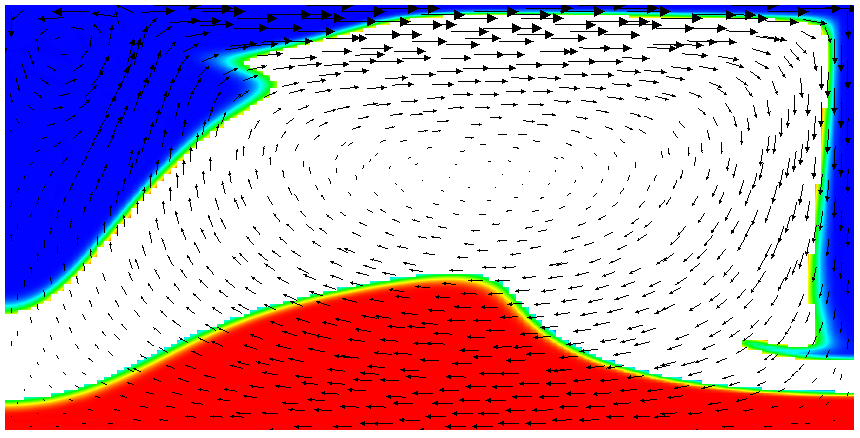
\includegraphics[width=0.3\textwidth]{cookbooks/composition_passive/doc/visit0009.png}
  \\
  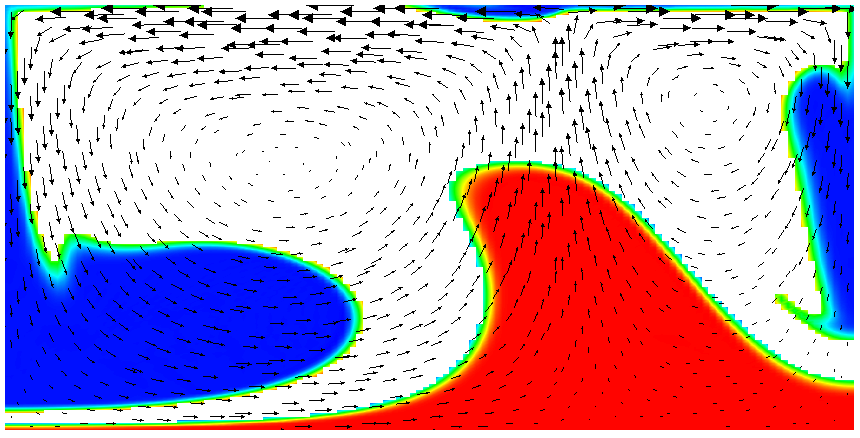
\includegraphics[width=0.3\textwidth]{cookbooks/composition_passive/doc/visit0010.png}
  \hfill
  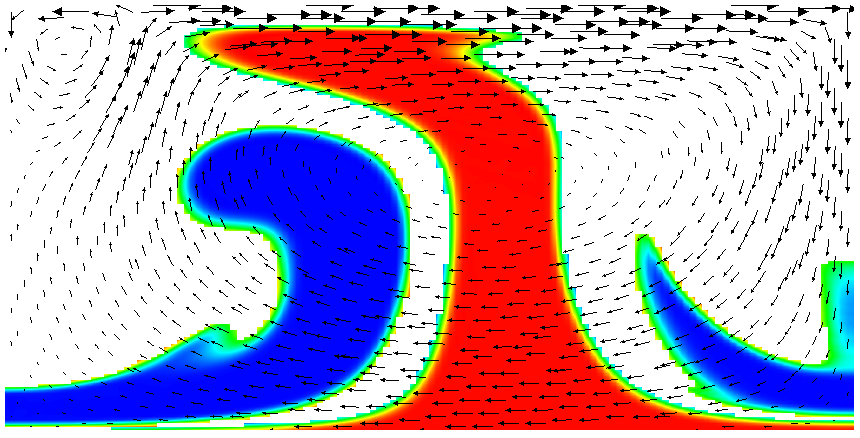
\includegraphics[width=0.3\textwidth]{cookbooks/composition_passive/doc/visit0012.png}
  \hfill
  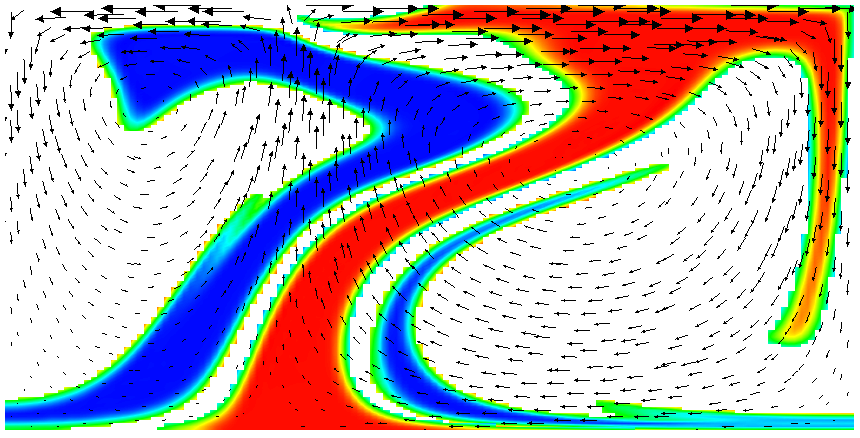
\includegraphics[width=0.3\textwidth]{cookbooks/composition_passive/doc/visit0014.png}
  \caption{\it Passive compositional fields: The figures show, at
    different times in the simulation, the velocity field along with
    those locations where the first compositional field is larger than
    0.5 (in red, indicating the locations where material from the bottom
    of the domain has gone) as well as where the second compositional
    field is larger than 0.5 (in blue, indicating material from the top
    of the domain. The results were obtained with two more global
    refinement steps compared to the
    \url{cookbooks/composition_passive/composition_passive.prm} input file.}
  \label{fig:compositional-passive}
\end{figure}

\begin{figure}
  \centering
  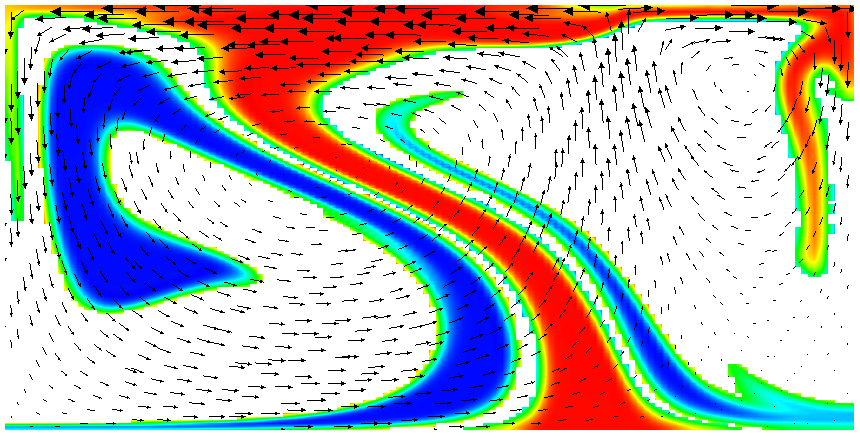
\includegraphics[height=0.3\textwidth]{cookbooks/composition_passive/doc/visit0015.png}
  \hfill
  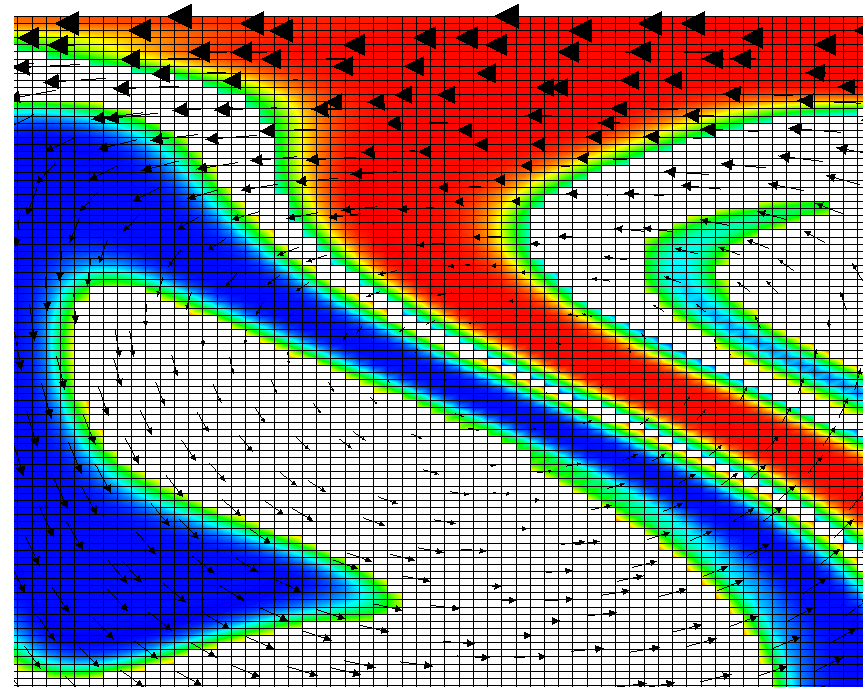
\includegraphics[height=0.3\textwidth]{cookbooks/composition_passive/doc/visit0017.png}
  \caption{\it Passive compositional fields: A later image of the simulation
    corresponding to the sequence shown in
    Fig.~\ref{fig:compositional-passive} (left) and zoom-in on the
    center, also showing the mesh (right).}
  \label{fig:compositional-passive-zoom}
\end{figure}


Fig.~\ref{fig:compositional-passive} shows one aspect of compositional
fields that occasionally makes them difficult to use for very long
time computations. The simulation shown here runs for 20 time units,
where every cycle of the spreading center at the top moving left and
right takes 4 time units, for a total of 5 such cycles. While this is
certainly no short-term simulation, it is obviously visible in the
figure that the interface between the materials has diffused over
time. Fig.~\ref{fig:compositional-passive-zoom} shows a zoom into the
center of the domain at the final time of the simulation. The
figure only shows values that are larger than 0.5, and it looks like
the transition from red or blue to the edge of the shown region is no
wider than 3 cells. This means that the computation is not overly
diffusive but it is nevertheless true that this method has difficulty
following long and thin filaments.%
\footnote{We note that this is no different for particles where the
  position of particles has to be integrated over time and is subject to
  numerical error. In simulations, their location is therefore not the
  exact one but also subject to a diffusive process resulting from
  numerical inaccuracies. Furthermore, in long thin filaments, the
  number of particles per cell often becomes too small and new particles
  have to be inserted; their properties are then interpolated from the
  surrounding particles, a process that also incurs a smoothing penalty.}
This is an area in which \aspect{} may see improvements in the future.


\begin{figure}
  \centering
  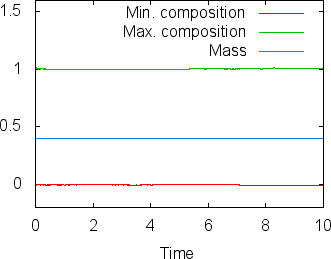
\includegraphics[width=0.4\textwidth]{cookbooks/composition_passive/doc/mass-composition-1.png}
  \caption{\it Passive compositional fields: Minimum and maximum of the first
  compositional variable over time, as well as the mass $m_1(t)=\int_\Omega c_1(\mathbf x,t)$ stored in this variable.}
  \label{fig:compositional-passive-mass}
\end{figure}

A different way of looking at the quality of compositional fields as opposed to
particles is to ask whether they conserve mass. In the current context, the
mass contained in the $i$th compositional field is $m_i(t)=\int_\Omega c_i(\mathbf x,t)$.
This can easily be achieve in the following way, by adding the \texttt{composition statistics}
postprocessor:

\lstinputlisting[language=prmfile]{cookbooks/composition_passive/doc/postprocess.part.prm.out}

While the scheme we use to advect the compositional fields is not strictly
conservative, it is almost perfectly so in practice. For example, in
the computations shown in this section (using two additional global mesh
refinements over the settings in the parameter file
\url{cookbooks/composition_passive/composition_passive.prm}), Fig.~\ref{fig:compositional-passive-mass}
shows the maximal and minimal values of the first compositional fields over time,
along with the mass $m_1(t)$ (these are all tabulated in columns of the
statistics file, see Sections~\ref{sec:running-overview} and \ref{sec:viz-stat}). While
the maximum and minimum fluctuate slightly due to the instability of the finite element
method in resolving discontinuous functions,
the mass appears stable at a value of 0.403646 (the exact value, namely the
area that was initially filled by each material, is 0.4; the difference is a
result of the fact that we can't exactly represent the step function on our
mesh with the finite element space). In fact, the maximal difference in this
value between time steps 1 and 500 is only $\num{1.1e-6}$. In other words,
these numbers show that the compositional field approach is almost exactly mass conservative.



% cookbooks/composition_active/

\paragraph{The active case.} The next step, of course, is to make the flow
actually depend on the composition. After all, compositional fields are not only
intended to indicate where material come from, but also to indicate the
properties of this material. In general, the way to achieve this is to write
material models where the density, viscosity, and other parameters depend on the
composition, taking into account what the compositional fields actually denote
(e.g., if they simply indicate the origin of material, or the concentration of
things like olivine, perovskite, \ldots). The construction of material models is
discussed in much greater detail in Section~\ref{sec:material-models}; we do not
want to revisit this issue here and instead choose -- once again -- the simplest
material model that is implemented in \aspect{}: the \texttt{simple} model.

The place where we are going to hook in a compositional dependence is the
density. In the \texttt{simple} model, the density is fundamentally described by
a material that expands linearly with the temperature; for small density
variations, this corresponds to a density model of the form
$\rho(T)=\rho_0(1-\alpha(T-T_0))$. This is, by virtue of its simplicity, the
most often considered density model. But the \texttt{simple} model also has a
hook to make the density depend on the first compositional field $c_1(\mathbf
x,t)$, yielding a dependence of the form
$\rho(T)=\rho_0(1-\alpha(T-T_0))+\gamma c_1$. Here, let us choose $\rho_0=1,
\alpha=0.01, T_0=0, \gamma=100$. The rest of our model setup will be as
in the passive case above. Because the temperature will be between zero and one,
the temperature induced density variations will be restricted to 0.01, whereas
the density variation by origin of the material is 100. This should make sure
that dense material remains at the bottom despite the fact that it is hotter
than the surrounding material.%
\footnote{The actual values do not matter as much here. They are chosen in such
a way that the system -- previously driven primarily by the velocity boundary
conditions at the top -- now also feels the impact of the density variations.
To have an effect, the buoyancy induced by the density difference between
materials must be strong enough to balance or at least approach the forces
exerted by whatever is driving the velocity at the top.}


This setup of the problem can be described using an input file that is almost
completely unchanged from the passive case. The only difference is the use of
the following section (the complete input file can be found in
\url{cookbooks/composition\_active/composition\_active.prm}:

\lstinputlisting[language=prmfile]{cookbooks/composition_active/doc/active.part.prm.out}

To debug the model, we will also want to visualize the density in our
graphical output files. This is done using the following addition to the
postprocessing section, using the \texttt{density} visualization plugin:
\lstinputlisting[language=prmfile]{cookbooks/composition_active/doc/postprocess.part.prm.out}

\begin{figure}
  \centering
  \centering
  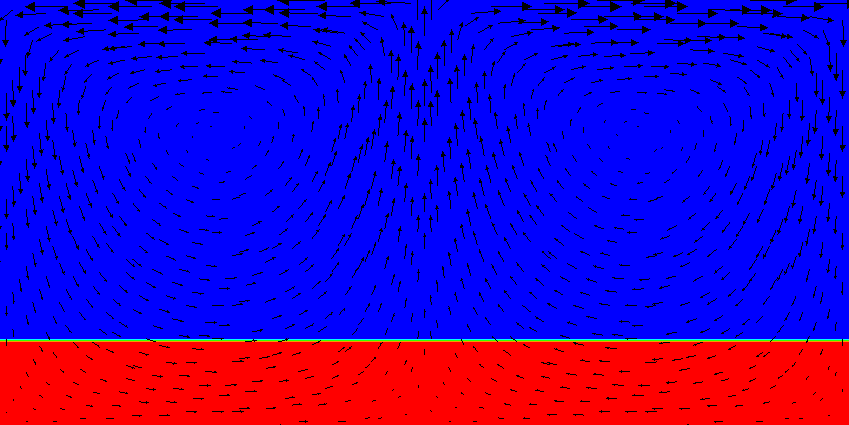
\includegraphics[width=0.3\textwidth]{cookbooks/composition_active/doc/visit0007.png}
  \hfill
  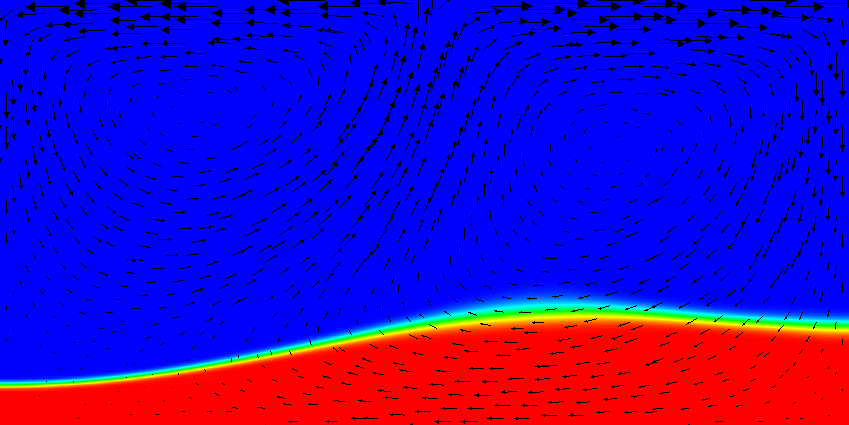
\includegraphics[width=0.3\textwidth]{cookbooks/composition_active/doc/visit0009.png}
  \hfill
  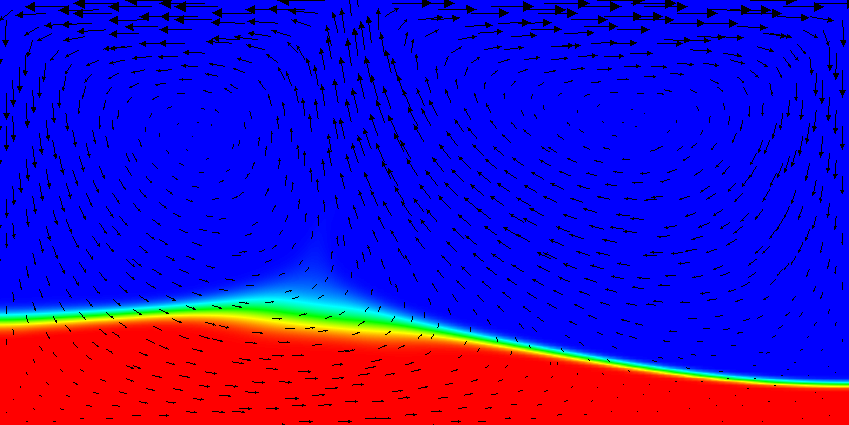
\includegraphics[width=0.3\textwidth]{cookbooks/composition_active/doc/visit0008.png}
  \caption{\it Active compositional fields: Compositional field 1 at the time
    $t=0, 10, 20$. Compared to the results shown in
    Fig.~\ref{fig:compositional-passive} it is clear that the heavy material
    stays at the bottom of the domain now. The effect of the density on the
    velocity field is also clearly visible by noting that at all three times
    the spreading center at the top boundary is in exactly the same position;
    this would result in exactly the same velocity field if the density and
    temperature were constant.}
  \label{fig:composition-active-composition}
\end{figure}

\begin{figure}
  \centering
  \includegraphics[width=0.3\textwidth]{cookbooks/composition_active/doc/visit0000.png}
  \hfill
  \includegraphics[width=0.3\textwidth]{cookbooks/composition_active/doc/visit0001.png}
  \hfill
  \includegraphics[width=0.3\textwidth]{cookbooks/composition_active/doc/visit0002.png}
  \\[6pt]
  \includegraphics[width=0.3\textwidth]{cookbooks/composition_active/doc/visit0003.png}
  \hfill
  \includegraphics[width=0.3\textwidth]{cookbooks/composition_active/doc/visit0004.png}
  \hfill
  \includegraphics[width=0.3\textwidth]{cookbooks/composition_active/doc/visit0006.png}
  \caption{\it Active compositional fields: Temperature fields at $t=0, 2, 4, 8,
  12, 20$. The black line is the isocontour line $c_1(\mathbf x,t)=0.5$
    delineating the position of the dense material at the bottom.}
  \label{fig:composition-active-temperature}
\end{figure}

Results of this model are visualized in
Figs.~\ref{fig:composition-active-composition} and \ref{fig:composition-active-temperature}. What is visible is
that over the course of the simulation, the material that starts at the bottom
of the domain remains there. This can only happen if the circulation is
significantly affected by the high density material once the interface starts
to become non-horizontal, and this is
indeed visible in the velocity vectors. As a second consequence, if the
material at the bottom does not move away, then there needs to be a different
way for the heat provided at the bottom to get through the bottom layer:
either there must be a secondary convection system in the bottom layer, or
heat is simply conducted. The pictures in the figure seem to suggest
that the latter is the case.

It is easy, using the
outline above, to play with the various factors that drive this system, namely:
\begin{itemize}
  \item The magnitude of the velocity prescribed at the top.
  \item The magnitude of the velocities induced by thermal buoyancy, as
  resulting from the magnitude of gravity and the thermal expansion coefficient.
  \item The magnitude of the velocities induced by compositional variability, as
  described by the coefficient $\gamma$ and the magnitude of gravity.
\end{itemize}
Using the coefficients involved in these considerations, it is trivially
possible to map out the parameter space to find which of these effects is
dominant. As mentioned in discussing the values in the input file, what is
important is the \textit{relative} size of these parameters, not the fact
that currently the density in the material at the bottom is 100 times larger
than in the rest of the domain, an effect that from a physical perspective
clearly makes no sense at all.




\paragraph{The active case with reactions.}

\textit{This section was contributed by Juliane Dannberg and Ren{\'e} Ga{\ss}m{\"o}ller}.

In addition, there are setups where one wants the compositional fields to interact with each other. One example would be material upwelling at a mid-ocean ridge and changing the composition to that of oceanic crust when it reaches a certain depth. In this cookbook, we will describe how this kind of behavior can be achieved by using the \texttt{composition reaction} function of the material model.

We will consider the exact same setup as in the previous paragraphs, except for the initial conditions and properties of the two compositional fields. There is one material that initially fills the bottom half of the domain and is less dense than the material above. In addition, there is another material that only gets created when the first material reaches the uppermost 20\% of the domain, and that has a higher density. This should cause the first material to move upwards, get partially converted to the second material, which then sinks down again. This means we want to change the initial conditions for the compositional fields:

\lstinputlisting[language=prmfile]{cookbooks/composition-reaction/doc/initial.part.prm.out}


Moreover, instead of the \texttt{simple} material model, we will use the \texttt{composition reaction} material model, which basically behaves in the same way, but can handle two active compositional field and a reaction between those two fields. In the input file, the user defines a depth and above this \texttt{reaction depth} the first compositional fields is converted to the second field. This can be done by changing the following section (the complete input file can be found in \url{cookbooks/composition-reaction.prm}).

\lstinputlisting[language=prmfile]{cookbooks/composition-reaction/doc/material.part.prm.out}

\begin{figure}
  \centering
  \includegraphics[width=0.3\textwidth]{cookbooks/composition-reaction/doc/0.png}
  \hfill
  \includegraphics[width=0.3\textwidth]{cookbooks/composition-reaction/doc/2.png}
  \hfill
  \includegraphics[width=0.3\textwidth]{cookbooks/composition-reaction/doc/4.png}
  \\[6pt]
  \includegraphics[width=0.3\textwidth]{cookbooks/composition-reaction/doc/8.png}
  \hfill
  \includegraphics[width=0.3\textwidth]{cookbooks/composition-reaction/doc/12.png}
  \hfill
  \includegraphics[width=0.3\textwidth]{cookbooks/composition-reaction/doc/20.png}
  \caption{\it Reaction between compositional fields: Temperature fields at $t=0, 2, 4, 8,
  12, 20$. The black line is the isocontour line $c_1(\mathbf x,t)=0.5$
    delineating the position of the material starting at the bottom and the white line is the    isocontour line $c_2(\mathbf x,t)=0.5$
    delineating the position of the material that is created by the reaction.}
  \label{fig:composition-reaction}
\end{figure}

Results of this model are visualized in
Fig~\ref{fig:composition-reaction}. What is visible is
that over the course of the simulation, the material that starts at the bottom
of the domain ascends, reaches the reaction depth and gets converted to the second material, which starts to sink down.



\subsubsection{Using particles}
\label{sec:cookbooks-particles}

Using compositional fields to trace where material has come from or is going to
has many advantages from a computational point of view. For example, the
numerical methods to advect along fields are well developed and we can do so at
a cost that is equivalent to one temperature solve for each of the compositional
fields. Unless you have many compositional fields, this cost is therefore
relatively small compared to the overall cost of a time step. Another advantage
is that the value of a compositional field is well defined at every point within
the domain. On the other hand, compositional fields over time diffuse initially
sharp interfaces, as we have seen in the images of the previous section.

At the same time, the geodynamics community has a history of using particles for
this purpose. Historically, this may have been because it is conceptually
simpler to advect along individual particles rather than whole fields, since it
only requires an ODE integrator rather than the stabilization techniques
necessary to advect fields. They also provide the appearance of no diffusion,
though this is arguable. Leaving aside the debate whether fields or particles are the
way to go, \aspect{} supports both: using fields and using particles.


% cookbooks/composition_passive_particles/

In order to advect particles along with the flow field, one just needs to
add the \texttt{particles} postprocessor to the list of postprocessors and specify
a few parameters. We do so in the
\url{cookbooks/composition_passive_particles/composition_passive_particles.prm} input file, which is otherwise
just a minor variation of the \url{cookbooks/composition_passive/composition_passive.prm} case
discussed in the previous Section~\ref{sec:cookbooks-composition}. In
particular, the postprocess section now looks like this:

\index[prmindex]{Number of particles}
\index[prmindexfull]{Postprocess!Particles!Number of particles}

\lstinputlisting[language=prmfile]{particles.part.prm.out}

The 1000 particles we are asking here are initially uniformly distributed
throughout the domain and are, at the end of each time step, advected along with
the velocity field just computed. (There are a number of options to decide which
method to use for advecting particles, see
Section~\ref{parameters:Postprocess/Particles}.)

If you run this cookbook, information about all particles will be written into
the output directory selected in the input file (as discussed in
\index[prmindex]{Output directory}
\index[prmindexfull]{Output directory}
Section~\ref{sec:running-overview}). In the current case, in addition to the
files already discussed there, a directory listing at the end of a run will show
several particle related files:
\begin{lstlisting}[frame=single,language=ksh]
aspect> ls -l output/
total 932
-rw-rw-r-- 1 bangerth bangerth  11134 Dec 11 10:08 depth_average.gnuplot
-rw-rw-r-- 1 bangerth bangerth  11294 Dec 11 10:08 log.txt
-rw-rw-r-- 1 bangerth bangerth 326074 Dec 11 10:07 parameters.prm
-rw-rw-r-- 1 bangerth bangerth 577138 Dec 11 10:07 parameters.tex
drwxrwxr-x 2 bangerth bangerth   4096 Dec 11 18:40 particles
-rw-rw-r-- 1 bangerth bangerth    335 Dec 11 18:40 particles.pvd
-rw-rw-r-- 1 bangerth bangerth    168 Dec 11 18:40 particles.visit
drwxr-xr-x 2 bangerth bangerth   4096 Dec 11 10:08 solution
-rw-rw-r-- 1 bangerth bangerth    484 Dec 11 10:08 solution.pvd
-rw-rw-r-- 1 bangerth bangerth    451 Dec 11 10:08 solution.visit
-rw-rw-r-- 1 bangerth bangerth   8267 Dec 11 10:08 statistics
\end{lstlisting}
Here, the \texttt{particles.pvd} and \texttt{particles.visit} files contain
a list of all visualization files from all processors and time steps. These
files can be loaded in much the same way as the \texttt{solution.pvd} and
\texttt{solution.visit} files that were discussed in Section~\ref{sec:viz}. The
actual data files -- possibly a large number, but not of much immediate interest
to users -- are located in the \texttt{particles} subdirectory.

Coming back to the example at hand, we can visualize the particles that
were advected along by opening both the field-based output files and the ones
that correspond to particles (for example, \texttt{output/solution.visit} and
\texttt{output/particles.visit}) and using a pseudo-color plot
for the particles, selecting the ``id'' of particles to color each particle.
By going to, for example, the output from the 72nd visualization output, this
then results in a plot like the one shown in
Fig.~\ref{fig:composition_passive_particles}.

\begin{figure}
  \centering
  \includegraphics[width=0.5\textwidth]{solution-00072.png}
  \caption{\it Passively advected quantities visualized through both a
  \label{fig:composition_passive_particles}
  compositional field and a set of 1,000 particles, at $t=7.2$.}
\end{figure}

The particles shown here are not too impressive in still pictures since they are
colorized by their particle number, which does not carry any particular meaning
other than the fact that it enumerates the particles.%
\footnote{Particles are enumerated in a way so that first the first processor
in a parallel computations numbers all of the particles on its first cell, then
its second cell, and so on; then the second processor does the same with
particles in the order of the cells it owns; etc. Thus, the ``id'' shown in the
picture is not just a random number, but rather shows the order of cells and
how they belonged to the processors that participated in the computation at the
time when particles were created. After some time, particles may of course have
become well mixed. In any case, this ordering is of no real practical use.}
The particle ``id'' can, however, be useful when viewing an animation of time steps.
There, the different colors of particles allows the eye to follow the motion of
a single particle. This is especially true if, after some time, particles have
become well mixed by the flow field and adjacent particles no longer have
similar colors. In any case, viewing such animations makes it rather intuitive
to understand a flow field, but it can of course not be reproduced in a static medium such as this manual.

In any case, we will see in the next section how to attach more interesting
information to particles, and how to visualize these.

\paragraph{Using particle properties.}

The particles in the above example only fulfill the purpose of
visualizing the convection pattern. A more meaningful use for
particles is to attach ``properties'' to them. A property consists of
one or more numbers (or vectors or tensors) that may either be set at
the beginning of the model run and stay constant, or are updated
during the model runtime. These properties can then be used for many
applications, e.g., storing an initial property (like the position, or
initial composition), evaluating a property at a defined particle path (like the
pressure-temperature evolution of a certain piece of rock), or by integrating a
quantity along a particle path (like the integrated strain a certain domain has
experienced).  We illustrate these properties in the cookbook
\url{cookbooks/composition_passive_particles/composition_passive_particles_properties.prm}, in which we add the
following lines to the \texttt{Particles} subsection (we also increase the number
of particles compared to the previous section to make the visualizations below
more obvious):

\lstinputlisting[language=prmfile]{particle-properties.part.prm.out}

These commands make sure that every particle will carry four different
properties (\texttt{function}, \texttt{pT path}, \texttt{initial
  position} and \texttt{initial composition}), some of which may be
scalars and others can have multiple components. (A full list of
particle properties that can currently be selected can be found in
Section~\ref{parameters:Postprocess/Particles}, and new particle
properties can be added as plugins as described in
Section~\ref{sec:write-plugin}.) The properties selected above do the following:

\begin{itemize}
\item \texttt{initial position:} This particle property simply stores
  the initial coordinates of the particle and then never changes them. This
  can be useful to compare the final position of a particle with its
  initial position and therefore determine how far certain domains traveled
  during the model runtime. Alternatively, one may want to simply visualize
  the norm of this vector property (i.e., the norm of the initial position,
  which is of course equal to the distance from the origin at which a particle
  started): in mantle simulations in spherical coordinates, the radius is
  indicative of which part of the mantle a particle comes from, and can
  therefore be used to visualize where material gets transported over the course
  of a simulation.
\item \texttt{initial composition:} This property uses the same
  method to initialize particle properties as is used to initialize
  the corresponding compositional fields. Using this, it stores the
  compositional field initialization values at the location where the particle
  started, and again never changes them. This is useful in the same
  context as shown for the field-based example in
  Section~\ref{sec:cookbooks-composition} where we would like to
  figure where materials ends up. In this case, one would set the
  initial composition to an indicator function for certain parts of
  the domain, and then set the initial composition property for the
  particles to match this composition. Letting the particles advect
  and at a later time visualizing this particle property will then
  show where particles came from. In cases where compositional
  variables undergo changes, e.g., by describing phase changes or
  chemical reactions, the ``initial composition'' property can also be
  useful to compare the final composition of a particle with its
  initial composition and therefore determine which regions underwent
  reactions such as those described in Section~\ref{sec:cookbooks-composition},
  and where the material that underwent this reaction got transported
  to.
\item \texttt{function:} This particle property can be used to assign
  to each particle values that are described based on a function of
  space. It provides an alternative way to set initial values if you
  don't want to first set a compositional field's initial values based
  on a function, and then copy these values via the ``initial
  composition'' property to particles. In the example above, we use
  the same function as for the compositional initial composition of
  field number one in
  Section~\ref{sec:cookbooks-composition}. Therefore, this property
  should behave identical to the compositional field (except that the
  compositional field may have a reaction term that this particle
  property does not), although the two are of course advected using
  very different methods. This allows to compare the error in particle
  position to the numerical diffusion of the compositional field.
\item \texttt{pT path:} This property is interesting in that the
  particle property's values always exactly mirror the pressure and
  temperature at the particle's current location. This does not seem
  to be very useful since the information is already
  available. However, because each particle has a unique id, one can
  select a particular particle and output its properties
  (including pressure and temperature based on the \texttt{pT path}
  property) at all time steps. This allows for the creation of a pressure-temperature 
  curve of a certain piece of rock. This property is interesting in many lithosphere 
  and crustal scale models, because it is determining the metamorphic reactions that 
  happen during deformation processes (e.g., in a subduction zone).
\end{itemize}


\begin{figure}
  \centering
  \phantom{.}
  \hfill
  \includegraphics[width=0.45\textwidth]{composition-C1.png}
  \hfill
  \includegraphics[width=0.45\textwidth]{particles-C1.png}
  \phantom{.}
  \\
  \phantom{.}
  \hfill
  \includegraphics[width=0.45\textwidth]{initial-position-00000.png}
  \hfill
  \includegraphics[width=0.45\textwidth]{initial-position-00199.png}
  \phantom{.}
  \caption{\it Passively advected particle properties visualized. Top row:
  Composition $C_1$ and particle property ``initial $C_1$''. The blue line in both
  figures is the 0.5-isocontour for the $C_1$ field. Bottom row: Norm of the
  ``initial position'' of particles at $t=0$ and $t=20$.}
  \label{fig:composition_passive_particles_properties}
\end{figure}

The results of all of these properties can of course be visualized.
Fig.~\ref{fig:composition_passive_particles_properties} shows some of the pictures
one can create with particles.
The top row shows both the composition field $C_1$ (along with the mesh on
which it is defined) and the corresponding ``initial $C_1$'' particle property,
at $t=7.2$. Because the compositional field does not undergo any reactions, it should of
course simply be the initial composition advected along with the flow field,
and therefore equal the values of the corresponding particle property. However,
field-based compositions suffer from diffusion. On the other hand, the amount
of diffusion can easily be decreased by mesh refinement.

The bottom of the figure shows the norm of the ``initial position'' property at
the initial time and at time $t=20$. These images therefore show how far from
the origin each of the particles shown was at the initial time.



% cookbooks/composition_active_particles/

\paragraph{Using active particles.}
In the examples above, particle properties passively track distinct
model properties.  These particle properties, however, may also be used
to actively influence the model as it runs.  For instance, a
composition-dependent material model may use particles' initial
composition rather than an advected compositional field. To make this
work -- i.e., to get information from particles that are located at
unpredictable locations, to the quadrature
points at which material models and other parts of the code need to
evaluate these properties -- we need to somehow get the values from
particles back to fields that can then be evaluated at any point where
this is necessary.
A slightly modified version of the active-composition cookbook (\url{cookbooks/composition_active/composition_active.prm}) illustrates how to use `active particles' in this manner.

This cookbook, \url{cookbooks/composition_active_particles/composition_active_particles.prm}, modifies two sections of the input file.  First, particles are added under the \texttt{Postprocess} section:

\lstinputlisting[language=prmfile]{cookbooks/composition_active_particles/doc/particles.part.prm.out}
Here, each particle will carry the \texttt{velocity} and
\texttt{initial composition} properties.  In order to use the particle initial composition value to modify the flow through the material model, we now modify the \texttt{Composition} section:

\lstinputlisting[language=prmfile]{cookbooks/composition_active_particles/doc/composition.part.prm.out}

What this does is the following: It says that there will be two
compositional fields, called \texttt{lower} and \texttt{upper}
(because we will use them to indicate material that comes from either
the lower or upper part of the domain). Next, the
\texttt{Compositional field methods} states that each of these fields
will be computed by interpolation from the particles (if we had left
this parameter at its default value, \texttt{field}, for each field,
then it would have solved an advection PDE in each time step, as we
have done in all previous examples).

In this case, we specify that both of the compositional fields are in
fact interpolated from particle properties in each time step. How this
is done is described in the fourth line. To understand it, it is
important to realize that particles and fields have matching names: We
have named the fields \texttt{lower} and \texttt{upper}, whereas the
properties that result from the \texttt{initial composition} entry in
the particles section are called \texttt{initial lower} and
\texttt{initial upper}, since they inherit the names of the fields.

The syntax for interpolation from particles to fields then
states that the \texttt{lower} field will be set to the interpolated
value of the \texttt{initial lower} particle property at the end of
each time step, and similarly
for the \texttt{upper} field. In turn, the
\texttt{initial composition} particle property was using the same
method that one would have used for the compositional field
initialization if these fields were actually advected along in each
time step.

In this model the given global refinement level (5), associated number of cells (1024) and 100,000 total particles produces an average particle-per-cell count slightly below 100.  While on the high end compared to most geodynamic studies using active particles, increasing the number of particles per cell further may alter the solution.  As with the numerical resolution, any study using active particles should systematically vary the number of particles per cell in order to determine this parameter's influence on the simulation.

\note{\aspect{}'s particle implementation is in a preliminary state. While the accuracy and scalability of the implementation is benchmarked, other limitations remain. This in particular means that it is not optimized for performance, and more than a few thousand particles per process can slow down a model significantly. Moreover, models with a highly adaptive mesh and many particles do encounter a significant slowdown, because \aspect{} only considers the number of degrees of freedom for load balancing across processes and not the number of particles. Therefore processes that compute the solution for coarse-grid regions have to process many more particles than other processes. Additionally, the checkpoint/restart functionality for particles is only implemented in models with a constant number of processes before and after the checkpoint and when the selected particle properties do not change. These limitations might be removed over time, but for current models the user should be aware of them.}



\subsubsection{Using a free surface}
\label{sec:cookbooks-freesurface}

\subsubsection{Using a free surface}
\label{sec:cookbooks-freesurface}
\textit{This section was contributed by Ian Rose}.

Free surfaces are numerically challenging but can be useful for self consistently
tracking dynamic topography and may be quite important as a boundary condition
for tectonic processes like subduction. The parameter file \url{cookbooks/free_surface/free_surface.prm} 
provides a simple example of how to set up a model with a free surface, as well 
as demonstrates some of the challenges associated with doing so.

\aspect{} supports models with a free surface using an Arbitrary Lagrangian-Eulerian 
framework (see Section~\ref{sec:freesurface}). Most of this is done internally, so you do not need to worry about the
details to run this cookbook.  Here we demonstrate the evolution of surface topography 
that results when a blob of hot material rises in the mantle, pushing up the free
surface as it does.  Usually the amplitude of free surface topography 
will be small enough that it is difficult to see with the naked eye in visualizations,
but the \texttt{topography} postprocessor can help by outputting the maximum and minimum 
topography on the free surface at every time step. 

The bulk of the parameter file for this cookbook is similar to previous ones in this manual.
We use initial temperature conditions that set up a hot blob of rock in the center of the 
domain.

The main addition is the \texttt{Mesh deformation} subsection.
In this subsection you need to give \aspect{} a comma
separated list of the boundary indicators where the `free surface' deformation should be applied.
In this case, we are dealing with the `top' boundary of a box in 2D.
There is another significant parameter that needs to be set here: the value for the stabilization parameter ``theta''.
If this parameter is zero, then there is no stabilization, and you are likely to
see instabilities develop in the free surface. If this parameter is one then it
will do a good job of stabilizing the free surface, but it may overly damp its 
motions. The default value is 0.5.

Also worth mentioning is the change to the initial time step size. Stability concerns typically 
mean that when making a model with a free surface you will want to take smaller 
time steps. In general just how much smaller will depend on the problem at hand
as well as the desired accuracy. Because this model has a very smooth time evolution
it is sufficient to reduce the time step size of the first few time steps.

Following are the sections in the input file specific to this testcase.  The full parameter
file may be found at \url{cookbooks/free_surface/free_surface.prm}.

\lstinputlisting[language=prmfile]{cookbooks/free_surface/doc/free_surface.part.prm.out}

Running this input file will produce results like those in Figure~\ref{fig:freesurface}.
The model starts with a single hot blob of rock which rises in the domain.  As it 
rises, it pushes up the free surface in the middle, creating a topographic high there.
This is similar to the kind of dynamic topography that you might see above a mantle 
plume on Earth.  As the blob rises and diffuses, it loses the buoyancy to push up 
the boundary, and the surface begins to relax.

After running the cookbook, you may modify it in a number of ways:
\begin{itemize}
\item Add a more complicated initial temperature field to see how that affects topography.
\item Add a high-viscosity lithosphere to the top using a compositional field to tamp down on topography.
\item Explore different values for the stabilization theta and the CFL number to understand the nature of when and why stabilization is necessary.
\item Try a model in a different geometry, such as spherical shells.
\end{itemize}

\begin{figure}
  \centering
  \includegraphics[height=0.25\textwidth]{cookbooks/free_surface/doc/free_surface_blob.png}
  \hfill
  \includegraphics[height=0.25\textwidth]{cookbooks/free_surface/doc/free_surface_topography.png}
  \caption{\it Evolution of surface topography due to a rising blob.  On the left is a 
           snapshot of the model setup.  The right shows the value of the highest 
           topography in the domain over 18 Myr of model time.  The topography peaks
           at 167 meters after 5.5 Myr.  This cookbook may be run with the
           \url{cookbooks/free_surface/free_surface.prm} input file.}
  \label{fig:freesurface}
\end{figure}


\subsubsection{Using a free surface in a model with a crust}
\label{sec:cookbooks-freesurfaceWC}

\subsubsection{Using a free surface in a model with a crust}
\label{sec:cookbooks-freesurfaceWC}
\textit{This section was contributed by William Durkin}.

This cookbook is a modification of the previous example that explores changes in the way topography develops when a 
highly viscous crust is added.  
In this cookbook, we use a material model in which the material changes from low
viscosity mantle to high viscosity crust at $z = z_j = \texttt{jump height}$,
i.e., the piecewise viscosity function is defined as
\begin{align*}
  \eta(z) = \left\{
    \begin{matrix}
      \eta_U & \text{for}\ z > z_j, \\
      \eta_L & \text{for}\ z  \le z_j.
    \end{matrix}
  \right.
\end{align*}
where $\eta_U$ and $\eta_L$ are the viscosities of the upper and lower layers,
respectively. This viscosity model can be implemented by creating a plugin that
is a small modification of the \texttt{simpler} material model (from which it
is otherwise simply copied). We call this material model ``SimplerWithCrust''.
In particular, what is necessary is an evaluation function that looks like this:
\begin{lstlisting}[frame=single,language=C++] 
    template <int dim>
    void
    SimplerWithCrust<dim>::
    evaluate(const typename Interface<dim>::MaterialModelInputs &in, 
             typename Interface<dim>::MaterialModelOutputs &out ) const
    {
      for (unsigned int i=0; i<in.n_evaluation_points(); ++i)
        {
          const double z = in.position[i][1];

          if (z>jump_height)
            out.viscosities[i] = eta_U;
          else
            out.viscosities[i] = eta_L;

          out.densities[i] = reference_density * (1.0 - thermal_expansion_coefficient * (in.temperature[i] - reference_temperature));
          out.thermal_expansion_coefficients[i] = thermal_expansion_coefficient;
          out.specific_heat[i] = reference_specific_heat;
          out.thermal_conductivities[i] = thermal_conductivity;
          out.compressibilities[i] = 0.0;
          out.entropy_derivative_pressure[i] = 0.0;
          out.entropy_derivative_temperature[i] = 0.0;
          for (unsigned int c=0; c<in.composition[i].size(); ++c)
            out.reaction_terms[i][c] = 0.0;
        }
    }
\end{lstlisting}

Additional changes make the new parameters \texttt{Jump height}, \texttt{Lower
viscosity}, and \texttt{Upper viscosity} available to the input parameter file,
and corresponding variables available in the class and used in the code snippet
above. The entire code can be found in
\url{cookbooks/free_surface_with_crust/plugin/simpler_with_crust.cc}. Refer to
Section~\ref{sec:plugins} for more information about writing and running
plugins.

The following changes are necessary compared to the input file from the
cookbook shown in Section~\ref{sec:cookbooks-freesurface} to include a crust:
\begin{itemize}
  \item Load the plugin implementing the new material model:
  \lstinputlisting[language=prmfile]{free_surface_with_crust.part1.prm.out}
  
  \item Declare values for the new parameters:
  \lstinputlisting[language=prmfile]{free_surface_with_crust.part2.prm.out}
  Note that the height of the interface at 170km is interpreted in the
  coordinate system in which the box geometry of this cookbook lives. The box
  has dimensions $500\si{km}\times 200\si{km}$, so an interface height of
  170km implies a depth of 30km.
\end{itemize}

The entire parameter file is located in
\url{cookbooks/free_surface_with_crust/free_surface_with_crust.prm}.

Running this input file generates a
crust that is 30 km thick and 1000 times as viscous as the lower layer.
Figure~\ref{fig:freesurfaceWC} shows that adding a crust to the model causes the maximum topography to both decrease and occur at a later time.
Heat flows through the system primarily by advection until the temperature anomaly reaches the base of the
crustal layer (approximately at the time for which Fig~\ref{fig:freesurfaceWC}
shows the temperature profile).
The crust's high viscosity reduces the temperature anomaly's velocity
substantially, causing it to affect the surface topography at a later time. Just
as the cookbook shown in Section~\ref{sec:cookbooks-freesurface}, the
topography returns to zero after some time.

\begin{figure}
  \centering
  \includegraphics[height=0.25\textwidth]{free_surface_with_crust.png}
  \hfill
  \includegraphics[height=0.25\textwidth]{topography.png}
  \caption{\it Adding a viscous crust to a model with surface topography. The
  thermal anomaly spreads horizontally as it collides with the highly viscous crust (left, white solid line). The addition of a crustal layer both dampens and delays the appearance of the topographic maximum and minimum (right).}
  \label{fig:freesurfaceWC}
\end{figure}


\subsubsection{Averaging material properties}
\label{sec:sinker-with-averaging}

\textit{The original motivation for the functionality discussed here, as well
  as the setup of the input file, were provided by Cedric Thieulot.}

Geophysical models are often characterized by abrupt and large jumps in material
properties, in particular in the viscosity. An example is a subducting, cold
slab surrounded by the hot mantle: Here, the strong
temperature-dependence of the viscosity will lead to a sudden jump in the
viscosity between mantle and slab. The length scale over which this jump happens
will be a few or a few tens of kilometers. Such length scales cannot be
adequately resolved in three-dimensional computations with typical meshes for
global computations.

Having large viscosity variations in models poses a variety of problems to
numerical computations. First, you will find that they lead to very long compute
times because our solvers and preconditioners break down. This may be
acceptable if it would at least lead to accurate solutions, but large viscosity
gradients lead also to large pressure gradients, and this in turn leads to over-
and undershoots in the numerical approximation of the gradient. We will
demonstrate both of these issues experimentally below.

One of the solution to such problems is the realization that one can mitigate
some of the effects by averaging material properties on each cell somehow
(see, for example, \cite{Bab08,Deu08,DMGT11,Thi15,TMK14}).
Before going into detail, it is important to realize that if we choose material
properties not per quadrature point when doing the integrals for forming the
finite element matrix, but per cell, then we will lose accuracy in the solution
in those cases where the solution is smooth. More specifically, we will likely
lose one or more orders of convergence. In other words, it would be a bad idea
to do this averaging unconditionally. On the other hand, if the solution has
essentially discontinuous gradients and kinks in the velocity field, then at
least at these locations we cannot expect a particularly high convergence order
anyway, and the averaging will not hurt very much either. In cases where
features of the solution that are due to strongly varying viscosities or other
parameters, dominate, we may then as well do the averaging per cell.

To support such cases, \aspect{} supports an operation where we evaluate the
material model at every quadrature point, given the temperature, pressure,
strain rate, and compositions at this point, and then either (i) use these
values, (ii) replace the values by their arithmetic average $\bar x = \frac 1N
\sum_{i=1}^N x_i$, (iii) replace the values by their harmonic average $\bar x
= \left(\frac 1N \sum_{i=1}^N \frac{1}{x_i}\right)^{-1}$, (iv) replace the
values by their geometric average $\bar x
= \left(\prod_{i=1}^N \frac{1}{x_i}\right)^{-1/N}$,
or (v) replace the
values by the largest value over all quadrature points on this cell. Option
(vi) is to project the values from the quadrature points to a bi- (in 2d) or
trilinear (in 3d) $Q_1$ finite element space on every cell, and then evaluate this
finite element representation again at the quadrature points. Unlike the other
five operations, the values we get at the quadrature points are not all the
same here.

We do this operation for all quantities that the material model computes,
i.e., in particular, the viscosity, the density, the compressibility, and the
various thermal and thermodynamic properties. In the first 4 cases, the
operation guarantees that the resulting material properties are bounded below
and above by the minimum and maximum of the original data set. In the last
case, the situation is a bit more complicated: The nodal values of the $Q_1$
projection are not necessarily bounded by the minimal or maximal original
values at the quadrature points, and then neither are the output values after
re-interpolation to the quadrature points. Consequently, after projection, we
limit the nodal values of the projection to the minimal and maximal original
values, and only then interpolate back to the quadrature points.

We demonstrate the effect of all of this with the ``sinker'' benchmark. This
benchmark is defined by a high-viscosity, heavy sphere at the center of a
two-dimensional box. This is achieved by defining a compositional field that is
one inside and zero outside the sphere, and assigning a compositional dependence
to the viscosity and density. We run only a single time step for this benchmark.
This is all modeled in the following input file that can also be found in
\url{cookbooks/sinker-with-averaging/sinker-with-averaging.prm}:
\lstinputlisting[language=prmfile]{cookbooks/sinker-with-averaging/doc/full.prm.out}

The type of averaging on each cell is chosen using this part of the input file:
\lstinputlisting[language=prmfile]{cookbooks/sinker-with-averaging/doc/harmonic.prm.out}
For the various different averaging options, and for different levels of mesh
refinement, Fig.~\ref{fig:sinker-with-averaging-pressure} shows
pressure plots that illustrate the problem with oscillations of the discrete
pressure. The important part of these plots is not that the solution looks
discontinuous -- in fact, the exact solution is discontinuous at the edge of the
circle\footnote{This is also easy to try experimentally -- use the input file
from above and select 5 global and 10 adaptive refinement steps, with the
refinement criteria set to \texttt{density}, then visualize the solution.} --
but the spikes that go far above and below the ``cliff'' in the pressure along
the edge of the circle. Without averaging, these spikes are obviously orders
of magnitude larger than the actual jump height. The spikes do not disappear
under mesh refinement nor averaging, but they become far less pronounced with
averaging. The results shown in the figure do not really allow to draw
conclusions as to which averaging approach is the best; a discussion of this
question can also be found in \cite{Bab08,Deu08,DMGT11,TMK14}).

A very pleasant side effect of averaging is that not only does the solution
become better, but it also becomes cheaper to compute.
Table~\ref{tab:sinker-with-averaging-iteration-counts} shows the
number of outer GMRES iterations when solving the Stokes
equations~\eqref{eq:stokes-1}--\eqref{eq:stokes-2}.%
\footnote{The outer iterations are only part of the problem. As discussed in
  \cite{KHB12}, each GMRES iteration requires solving a linear system with the
  elliptic operator $-\nabla \cdot 2 \eta \varepsilon(\cdot)$. For highly
  heterogeneous models, such as the one discussed in the current section, this
  may require a lot of Conjugate Gradient iterations. For example, for 8
  global refinement steps, the 30+188 outer iterations without averaging shown
  in Table~\ref{tab:sinker-with-averaging-iteration-counts} require a total of
  22,096 inner CG iterations for the elliptic block (and a total of 837 for the
  approximate Schur complement). Using harmonic averaging, the 30+26 outer
  iterations require only 1258 iterations on the elliptic block (and 84 on the
  Schur complement). In other words, the number of inner iterations per outer
  iteration (taking into account the split into ``cheap'' and ``expensive''
  outer iterations, see \cite{KHB12}) is reduced from 117 to 47 for the
  elliptic block and from 3.8 to 1.5 for the Schur complement.}
The implication of these results is that the averaging gives us a solution
that not only reduces the degree of pressure over- and undershoots, but is also
significantly faster to compute: for example, the total run time for 8 global
refinement steps is reduced from 5,250s for no averaging to 358s for harmonic
averaging.


\begin{figure}[htb]
  \centering
  \begin{tabular}{cccccc}
    \includegraphics[width=0.14\textwidth]{cookbooks/sinker-with-averaging/q2q1/sinker-7-none.png}
    &
    \includegraphics[width=0.14\textwidth]{cookbooks/sinker-with-averaging/q2q1/sinker-7-arithmetic.png}
    &
    \includegraphics[width=0.14\textwidth]{cookbooks/sinker-with-averaging/q2q1/sinker-7-harmonic.png}
    &
    \includegraphics[width=0.14\textwidth]{cookbooks/sinker-with-averaging/q2q1/sinker-7-geometric.png}
    &
    \includegraphics[width=0.14\textwidth]{cookbooks/sinker-with-averaging/q2q1/sinker-7-largest.png}
    &
    \includegraphics[width=0.14\textwidth]{cookbooks/sinker-with-averaging/q2q1/sinker-7-project.png}
    \\
    $[-45.2,45.2]$
    &
    $[-2.67,2.67]$
    &
    $[-3.58,3.58]$
    &
    $[-3.57,3.57]$
    &
    $[-1.80,1.80]$
    &
    $[-2.77,2.77]$
    \\
    \\
    \includegraphics[width=0.14\textwidth]{cookbooks/sinker-with-averaging/q2q1/sinker-8-none.png}
    &
    \includegraphics[width=0.14\textwidth]{cookbooks/sinker-with-averaging/q2q1/sinker-8-arithmetic.png}
    &
    \includegraphics[width=0.14\textwidth]{cookbooks/sinker-with-averaging/q2q1/sinker-8-harmonic.png}
    &
    \includegraphics[width=0.14\textwidth]{cookbooks/sinker-with-averaging/q2q1/sinker-8-geometric.png}
    &
    \includegraphics[width=0.14\textwidth]{cookbooks/sinker-with-averaging/q2q1/sinker-8-largest.png}
    &
    \includegraphics[width=0.14\textwidth]{cookbooks/sinker-with-averaging/q2q1/sinker-8-project.png}
    \\
    $[-44.5,44.5]$
    &
    $[-5.18,5.18]$
    &
    $[-5.09,5.09]$
    &
    $[-5.18,5.18]$
    &
    $[-5.20,5.20]$
    &
    $[-7.99,7.99]$
  \end{tabular}
  \caption{\it Visualization of the pressure field for the ``sinker''
    problem. Left to right: No averaging, arithmetic averaging, harmonic
    averaging, geometric averaging, pick largest, project to $Q_1$. Top: 7
    global refinement steps. Bottom: 8 global refinement steps. The minimal and maximal pressure
    values are indicated below every picture. This range is symmetric because
    we enforce that the average of the pressure equals zero. The color scale
    is adjusted to show only values between $p=-3$ and $p=3$.}
  \label{fig:sinker-with-averaging-pressure}
\end{figure}

\begin{table}[htb]
  \center
  \begin{tabular}{|c|cccccc|}
    \hline
    \# of global & no averaging & arithmetic & harmonic & geometric
    & pick & project \\
    refinement steps & & averaging & averaging &
    averaging & largest & to $Q_1$
    \\ \hline
    4          & 30+64   & 30+13      & 30+10    & 30+12 & 30+13 & 30+15 \\
    5          & 30+87   & 30+14      & 30+13    & 30+14 & 30+14 & 30+16 \\
    6          & 30+171  & 30+14      & 30+15    & 30+14 & 30+15 & 30+17 \\
    7          & 30+143  & 30+27      & 30+28    & 30+26 & 30+26 & 30+28 \\
    8          & 30+188  & 30+27      & 30+26    & 30+27 & 30+28 & 30+28 \\ \hline
  \end{tabular}
  \caption{\it Number of outer GMRES iterations to solve the Stokes equations
  for various numbers of global mesh refinement steps and for different
  material averaging operations. The GMRES solver first tries to run 30
  iterations with a cheaper preconditioner before switching to a more expensive
  preconditioner (see Section~\ref{parameters:Nonlinear solver tolerance}).}
  \label{tab:sinker-with-averaging-iteration-counts}
\end{table}
Such improvements carry over to more complex and realistic models. For
example, in a simulation of flow under the East African Rift by Sarah Stamps,
using approximately 17 million unknowns and run on 64 processors, the number
of outer and inner iterations is reduced from 169 and 114,482 without
averaging to 77 and 23,180 with harmonic averaging, respectively.
This translates into a reduction of run-time from 145 hours to 17
hours. Assessing the accuracy of the answers is of course more complicated in
such cases because we do not know the exact solution. However, the results
without and with averaging do not differ in any significant way.

A final comment is in order. First, one may think that the results should be
better in cases of discontinuous pressures if the numerical approximation
actually allowed for discontinuous pressures. This is in fact possible: We can
use a finite element in which the pressure space contains piecewise constants
(see Section~\ref{parameters:Discretization}). To do so, one simply needs to add
the following piece to the input file:
\lstinputlisting[language=prmfile]{cookbooks/sinker-with-averaging/doc/conservative.prm.out}
Disappointingly, however, this makes no real difference: the pressure
oscillations are no better (maybe even worse) than for the standard Stokes
element we use, as shown in
Fig.~\ref{fig:sinker-with-averaging-pressure-q2q1iso} and
Table~\ref{tab:sinker-with-averaging-max-pressure-q2q1iso}. Furthermore, as
shown in Table~\ref{tab:sinker-with-averaging-iteration-counts-q2q1iso}, the
iteration numbers are also largely unaffected if any kind of averaging is used
-- though they are far worse using the locally conservative discretization if no
averaging has been selected. On the positive side, the visualization of the
discontinuous pressure finite element solution makes it much easier to see
that the true pressure is in fact discontinuous along the edge of the circle.

\begin{figure}[htb]
  \centering
  \begin{tabular}{cccccc}
    \includegraphics[width=0.14\textwidth]{cookbooks/sinker-with-averaging/q2q1plus/sinker-7-none.png}
    &
    \includegraphics[width=0.14\textwidth]{cookbooks/sinker-with-averaging/q2q1plus/sinker-7-arithmetic.png}
    &
    \includegraphics[width=0.14\textwidth]{cookbooks/sinker-with-averaging/q2q1plus/sinker-7-harmonic.png}
    &
    \includegraphics[width=0.14\textwidth]{cookbooks/sinker-with-averaging/q2q1plus/sinker-7-geometric.png}
    &
    \includegraphics[width=0.14\textwidth]{cookbooks/sinker-with-averaging/q2q1plus/sinker-7-pick-largest.png}
    &
    \includegraphics[width=0.14\textwidth]{cookbooks/sinker-with-averaging/q2q1plus/sinker-7-project-to-Q1.png}
    \\
    \includegraphics[width=0.14\textwidth]{cookbooks/sinker-with-averaging/q2q1plus/sinker-8-none.png}
    &
    \includegraphics[width=0.14\textwidth]{cookbooks/sinker-with-averaging/q2q1plus/sinker-8-arithmetic.png}
    &
    \includegraphics[width=0.14\textwidth]{cookbooks/sinker-with-averaging/q2q1plus/sinker-8-harmonic.png}
    &
    \includegraphics[width=0.14\textwidth]{cookbooks/sinker-with-averaging/q2q1plus/sinker-8-geometric.png}
    &
    \includegraphics[width=0.14\textwidth]{cookbooks/sinker-with-averaging/q2q1plus/sinker-8-pick-largest.png}
    &
    \includegraphics[width=0.14\textwidth]{cookbooks/sinker-with-averaging/q2q1plus/sinker-8-project-to-Q1.png}
  \end{tabular}
  \caption{\it Visualization of the pressure field for the ``sinker''
    problem. Like Fig.~\ref{fig:sinker-with-averaging-pressure} but using the
    locally conservative, enriched Stokes element. Pressure values are shown
    in Table~\ref{tab:sinker-with-averaging-max-pressure-q2q1iso}.}
  \label{fig:sinker-with-averaging-pressure-q2q1iso}
\end{figure}


\begin{table}[htb]
  \center
  \begin{tabular}{|c|cccccc|}
    \hline
    \# of global & no averaging & arithmetic & harmonic & geometric
    & pick & project \\
    refinement steps & & averaging & averaging &
    averaging & largest & to $Q_1$
    \\ \hline
    4 & 66.32 & 2.66 & 2.893 & 1.869 & 3.412 & 3.073 \\
    5 & 81.06 & 3.537 & 4.131 & 3.997 & 3.885 & 3.991 \\
    6 & 75.98 & 4.596 & 4.184 & 4.618 & 4.568 & 5.093 \\
    7 & 84.36 & 4.677 & 5.286 & 4.362 & 4.635 & 5.145 \\
    8 & 83.96 & 5.701 & 5.664 & 4.686 & 5.524 & 6.42 \\ \hline
  \end{tabular}
  \caption{\it Maximal pressure values for the ``sinker'' benchmark, using the
  locally conservative, enriched Stokes element. The corresponding
  pressure solutions are shown in
  Fig.~\ref{fig:sinker-with-averaging-pressure-q2q1iso}.}
  \label{tab:sinker-with-averaging-max-pressure-q2q1iso}
\end{table}


\begin{table}[htb]
  \center
  \begin{tabular}{|c|cccccc|}
    \hline
    \# of global & no averaging & arithmetic & harmonic & geometric
    & pick & project \\
    refinement steps & & averaging & averaging &
    averaging & largest & to $Q_1$
    \\ \hline
    4 & 30+376 & 30+16 & 30+12 & 30+14 & 30+14 & 30+17 \\
    5 & 30+484 & 30+16 & 30+14 & 30+14 & 30+14 & 30+16 \\
    6 & 30+583 & 30+16 & 30+17 & 30+14 & 30+17 & 30+17 \\
    7 & 30+1319 & 30+27 & 30+28 & 30+26 & 30+28 & 30+28 \\
    8 & 30+1507 & 30+28 & 30+27 & 30+28 & 30+28 & 30+29  \\ \hline
  \end{tabular}
  \caption{\it Like Table~\ref{tab:sinker-with-averaging-iteration-counts}, but
  using the locally conservative, enriched Stokes element.}
  \label{tab:sinker-with-averaging-iteration-counts-q2q1iso}
\end{table}


\subsubsection{Prescribed internal velocity constraints}
\label{sec:prescribed-velocities}
\textit{This section was contributed by Jonathan Perry-Houts}

In cases where it is desirable to investigate the behavior of one part of the model
domain but the controlling physics of another part is difficult to capture,
such as corner flow in subduction zones, it may be useful to force the desired
behavior in some parts of the model domain and solve for the resulting flow
everywhere else. This is possible through the use of \aspect{}'s ``signal'' mechanism,
as documented in Section~\ref{sec:extending-signals}.

Internally, \aspect{} adds ``constraints'' to the finite element system for boundary
conditions and hanging nodes. These are places in the finite element system where
certain solution variables are required to match some prescribed value. Although it
is somewhat mathematically inadmissible to prescribe constraints on nodes inside
the model domain, $\Omega$, it is nevertheless possible so long as the prescribed
velocity field fits in to the finite element's solution space, and satisfies the
other constraints (i.e., is divergence free).

Using \aspect{}'s signals mechanism, we write a shared library which provides a
``slot'' that listens for the signal which is triggered after the regular model
constraints are set, but before they are ``distributed.''

As an example of this functionality, below is a plugin which allows the user to prescribe
internal velocities with functions in a parameter file:
\lstinputlisting[language=C++]{../../cookbooks/prescribed_velocity/prescribed_velocity.cc}

The above plugin can be compiled with \texttt{cmake . \&\& make} in the
\url{cookbooks/prescribed_velocity} directory. It can be loaded in a parameter file
as an ``Additional shared library.'' By setting parameters like those shown below,
it is possible to produce many interesting flow fields such as the ones visualized in
(Figure~\ref{fig:prescribed-velocity}).
\lstinputlisting[language=prmfile]{cookbooks/prescribed_velocity/doc/minimal.prm.out}

\begin{figure}
    \centering
  \subfigure[]{
    \includegraphics[width=.48\textwidth]{cookbooks/prescribed_velocity/doc/corner_flow.png}}
  ~
  \subfigure[]{
    \includegraphics[width=.48\textwidth]{cookbooks/prescribed_velocity/doc/circle.png}}
    \caption{\it Examples of flows with prescribed internal velocities, as described in Section \ref{sec:prescribed-velocities}.}
    \label{fig:prescribed-velocity}
\end{figure}

\subsubsection{Prescribing internal velocity constraints with ASCII files}
\label{sec:prescribed-velocities-ascii-data}
\textit{This section was contributed by Bob Myhill}

Building on \ref{sec:prescribed-velocities}, the \url{cookbooks/prescribed_velocity_ascii_data}
directory contains a plugin which uses an ASCII data file to specify where to prescribe
internal velocities. Velocities are prescribed wherever the field value indicated by the ASCII data file
is greater than 0.5. As before, the plugin is loaded in parameter files as an additional shared library:
\lstinputlisting[language=prmfile]{cookbooks/prescribed_velocity_ascii_data/doc/prescribed_velocity_ascii_data.prm.0.out}

An example parameter file using this plugin can be found at
\url{cookbooks/prescribed_velocity_ascii_data/prescribed_velocity_ascii_data.prm}.
In this file, the velocities are constrained to be zero within the letters ``ASPECT'' (Figure~\ref{fig:prescribed-velocity-ascii-data-init}).
The part of this file which provides the location of the ASCII file and the
prescribed velocity field function is:
\lstinputlisting[language=prmfile]{cookbooks/prescribed_velocity_ascii_data/doc/prescribed_velocity_ascii_data.prm.1.out}
A temperature gradient is applied within the letters, while the temperature field outside the letters is set to be constant.
This initial temperature field is specified by another ASCII data file:
\lstinputlisting[language=prmfile]{cookbooks/prescribed_velocity_ascii_data/doc/prescribed_velocity_ascii_data.prm.2.out}
These two ASCII data files are generated from \texttt{aspect\_name.png} by the python file \texttt{make\_ascii\_files\_from\_png.py},
both of which can be found in the same directory as the parameter file.

\begin{figure}
    \centering
    \includegraphics[width=\textwidth]{cookbooks/prescribed_velocity_ascii_data/doc/prescribed_velocities_ascii_data_initial_conditions.png}
    \caption{\it Initial composition and temperature conditions for the prescribed velocity ascii data cookbook,
             as described in Section \ref{sec:prescribed-velocities-ascii-data}.}
    \label{fig:prescribed-velocity-ascii-data-init}
\end{figure}

During the simulation, excess heat diffuses out from the tops of the letters, and
into the bases of the letters. The temperature gradients in the unconstrained
part of the domain then generate convective flow. Figure~\ref{fig:prescribed-velocity-ascii-data}
illustrates the resulting flow field.
\begin{figure}
    \centering
    \includegraphics[width=0.8\textwidth]{cookbooks/prescribed_velocity_ascii_data/doc/prescribed_velocity_ascii_data.png}
    \caption{\it Convective flow around the letters ASPECT, within which velocities are prescribed to be zero, as described in Section \ref{sec:prescribed-velocities-ascii-data}.}
    \label{fig:prescribed-velocity-ascii-data}
\end{figure}


\subsubsection{Artificial viscosity smoothing}
\label{sec:artificial-viscosity-smoothing}
\textit{This section was contributed by Ryan Grove}

Standard finite element discretizations of advection-diffusion equations introduce unphysical oscillations around steep gradients. Therefore, stabilization must be added to the discrete formulation to obtain correct solutions. In ASPECT, we use the Entropy Viscosity scheme developed by Guermond et al.~in the paper \cite{guer11}. In this scheme, an artificial viscosity is calculated on every cell and used to try to combat these oscillations that cause unwanted overshoot and undershoot.  More information about how \aspect{} does this is located at \url{https://dealii.org/developer/doxygen/deal.II/step_31.html}.

Instead of just looking at an individual cell's artificial viscosity, improvements in the minimizing of the oscillations can be made by smoothing.  Smoothing is the act of finding the maximum artificial viscosity taken over a cell $T$ and the neighboring cells across the faces of $T$, i.e.,
\begin{equation*}
\bar{v_h}(T) = \max_{K \in N(T)} v_h(K)
\end{equation*}
where $N(T)$ is the set containing $T$ and the neighbors across the faces of $T$.

This feature can be turned on by setting the \hyperref[parameters:Discretization/Stabilization parameters/Use artificial viscosity smoothing]{Use artificial viscosity smoothing} flag inside the \hyperref[parameters:Discretization/Stabilization_20parameters]{Stabilization} subsection inside the \hyperref[parameters:Discretization]{Discretization} subsection in your parameter file.

To show how this can be used in practice, let us consider the simple convection in a quarter of a 2d annulus cookbook in Section \ref{sec:shell-simple-2d}, a radial compositional field was added to help show the advantages of using the artificial viscosity smoothing feature.

By applying the following changes shown below to the parameters of the already existing file \begin{verbatim}cookbooks/shell_simple_2d.prm, \end{verbatim}
\lstinputlisting[language=prmfile]{cookbooks/shell_simple_2d_smoothing/doc/shell_simple_2d_smoothing.part.prm.out}
it is possible to produce pictures of the simple convection in a quarter of a 2d annulus such as the ones visualized in
Figure~\ref{fig:smoothing}.

\begin{figure}
    \centering
  \subfigure[]{
    \includegraphics[width=.48\textwidth]{cookbooks/shell_simple_2d_smoothing/doc/with_smoothing.png}}
  ~
  \subfigure[]{
    \includegraphics[width=.48\textwidth]{cookbooks/shell_simple_2d_smoothing/doc/without_smoothing.png}}
    \caption{\it Artificial viscosity smoothing: Example of the output of two similar runs.  The run on the left has the artificial viscosity smoothing turned on and the run on the right does not, as described in Section \ref{sec:artificial-viscosity-smoothing}.}
    \label{fig:smoothing}
\end{figure}


% cookbooks/finite_strain/
\subsubsection{Tracking finite strain}
\label{sec:finite-strain}
\textit{This section was contributed by Juliane Dannberg and Rene Gassm\"{o}ller}

\note{In this section, following \cite{Becker2003, dahlen1998theoretical}, we denote the velocity gradient tensor as $\mathbf G$, where $\mathbf G = \nabla \mathbf u^T$,
and $\mathbf u$ is the velocity. Note that this is different from the definition of the strain rate $\epsilon(\mathbf u)$, which only contains the symmetric part of $\mathbf G$. We then denote the deformation gradient (or deformation) tensor by $\mathbf F$, where $\mathbf F$ is the tensor that
deforms an initial state $\mathbf x$ into an deformed state $\mathbf r = \mathbf F \mathbf x$.}

In many geophysical settings, material properties, and in particular the rheology, do not only depend
on the current temperature, pressure and strain rate, but also on the history of the system.
This can be incorporated in ASPECT models by tracking history variables through compositional fields.
In this cookbook, we will show how to do this by tracking the strain that idealized little grains of finite size accumulate over time at every
(Lagrangian) point in the model.

Here, we use a material model plugin that defines the compositional fields as the components of the deformation
gradient tensor $\mathbf F_{ij}$, and modifies the right-hand side of
the corresponding advection equations to accumulate strain over time. This is done by adjusting the
\verb!out.reaction_terms! variable:
\lstinputlisting[language=C++]{finite_strain.cc}

Let us denote the accumulated deformation at time step $n$ as $\mathbf F^n$. We can calculate its time derivative
as the product of two tensors, namely the current velocity gradient $\mathbf G_{ij} = \frac{\partial u_i}{\partial x_j}$ and the deformation gradient $\mathbf F^{n-1}$ accumulated up to the previous time step, in other words $\frac{\partial \mathbf F}{\partial t} = \mathbf G \mathbf F$, and $\mathbf F^0 = \mathbf I$, with $\mathbf I$ being the identity tensor.
While we refer to other studies \cite{McKenzie1983, dahlen1998theoretical, Becker2003} for a derivation of
this relationship, we can give an intuitive example for the necessity to apply the velocity gradient to the already accumulated deformation, instead of simply integrating the velocity gradient over time. Consider a simple one-dimensional ``grain'' of length $1.0$, in which case the deformation tensor only has one component, the compression in $x$-direction. If one embeds this grain into a convergent flow field for a compressible medium where the dimensionless velocity gradient is $-0.5$  (e.g. a velocity of zero at its left end at $x=0.0$, and a velocity of $-0.5$ at its right end at $x=1.0$), simply integrating the velocity gradient would suggest that the grain reaches a length of zero after two units of time, and would then ``flip'' its orientation, which is clearly non-physical.
What happens instead can be seen by solving the equation of motion for the right end of the grain $\frac{dx}{dt} = v = -0.5 x$. Solving this equation for $x$ leads to $x(t) = e^{-0.5t}$. This is therefore also the solution for $\mathbf F$ since $\mathbf F x$ transforms the initial position of $x(t=0)=1.0$ into the deformed position of $x(t=1) = e^{-0.5}$, which is the definition of $\mathbf F$.

In more general cases a visualization of $\mathbf F$ is not intuitive, because it contains rotational components that represent a rigid body rotation without deformation. Following \cite{Becker2003} we can polar-decompose the tensor into a positive-definite and symmetric left stretching tensor $\mathbf L$, and an orthogonal rotation tensor $\mathbf Q$, as $\mathbf F = \mathbf L \mathbf Q$, therefore $\mathbf L^2 = \mathbf L \mathbf L^T = \mathbf F \mathbf F^T$. The left stretching tensor $\mathbf L$ (or finite strain tensor) then describes the deformation we are interested in, and its eigenvalues $\lambda_i$ and eigenvectors $\mathbf e_i$ describe the length and orientation of the half-axes of the finite strain ellipsoid. Moreover, we will represent the amount of relative stretching at every point by the ratio $\ln(\lambda_1/\lambda_2)$, called the \textit{natural strain} \cite{Ribe1992}.

The full plugin implementing the integration of $\mathbf F$ can be found in \url{cookbooks/finite_strain/finite_strain.cc} and can be compiled
with \texttt{cmake . \&\& make} in the \url{cookbooks/finite_strain} directory.
It can be loaded in a parameter file as an ``Additional shared library'', and selected as material
model. As it is derived from the ``simple'' material model, all input parameters for the material
properties are read in from the subsection \texttt{Simple model}.
\lstinputlisting[language=prmfile]{finite_strain.part.prm.out}

\begin{figure}
    \centering
    \includesvg[width=0.75\textwidth]{finite_strain.svg}
    \caption{\it Accumulated finite strain in an example convection model, as described in Section
             \ref{sec:finite-strain} at a time of 67.6~Ma. Top panel: Temperature distribution. Bottom panel:
             Natural strain distribution. Additional black crosses are the scaled eigenvectors of the
             stretching tensor $\mathbf L$, showing the direction of stretching and compression.}
    \label{fig:finite_strain}
\end{figure}

The plugin was tested against analytical solutions for the deformation gradient tensor in simple and pure shear as described in \url{benchmarks/finite_strain/pure_shear.prm} and \url{benchmarks/finite_strain/simple_shear.prm}.

We will demonstrate its use at the example of a 2D Cartesian convection model (Figure~\ref{fig:finite_strain}):
Heating from the bottom leads to the ascent of plumes from the boundary layer (top panel), and the
amount of stretching is visible in the distribution of natural strain (color in lower panel).
Additionally, the black crosses show the direction of stretching and compression (the eigenvectors of $\mathbf L$).
Material moves to the sides at the top of the plume head, so that it is shortened in vertical
direction (short vertical lines) and stretched in horizontal direction (long horizontal lines).
The sides of the plume head show the opposite effect. Shear occurs mostly at the
edges of the plume head, in the plume tail, and in the bottom boundary layer
(black areas in the natural strain distribution).

The example used here shows how history variables can be integrated up over the model evolution.
While we do not use these variables actively in the computation (in our example, there is no
influence of the accumulated strain on the rheology or any other material property), it would be trivial
to extend this material model in a way that material properties depend on the integrated strain:
Because the values of the compositional fields are part of what the material model gets as inputs,
they can easily be used for computing material model outputs such as the viscosity.

\note{In this model we present the use of multiple compositional fields for other purposes than chemical composition.
It would have been feasible to run the same model with particles that track the deformation gradient, as
additionally implemented and tested in the simple shear and pure shear benchmarks mentioned in this section.
Both approaches have specific advantages, and for scientific computations one needs to evaluate the more suitable
strategy. Compositional fields cover the whole domain, but are affected by numerical diffusion, effectively reducing the
maximum accumulated strain. Particles only provide finite strain values at discrete positions, but can, if this is desired, be used in
fewer numbers and only a part of the model domain (and are much faster in this case). If however
there needs to be a large number of particles (possibly because they are used for other purposes as well), then they
can be much more expensive. Both approaches can be used to actively influence the rheology in the material model.}


% cookbooks/geomio
\subsubsection{Reading in compositional initial composition files generated with geomIO}
\label{sec:geomio}
\textit{This section was contributed by Juliane Dannberg}

\note{This cookbook is based on a developer version of geomIO from July 2016. In the meantime, the development of
geomIO continued, and there is now a publication\cite{bauvillegeomio} that describes its features and how they can be used in more detail.}

Many geophysical setups require initial conditions with several different materials and complex geometries.
Hence, sometimes it would be easier to generate the initial geometries of the materials as a drawing instead
of by writing code. The MATLAB-based library geomIO (\url{https://bitbucket.org/geomio/geomio}, \cite{bauvillegeomio}) provides a convenient tool
to convert a drawing generated with the vector graphics editor Inkscape (\url{https://inkscape.org/en/}) to a data
file that can be read into \aspect{}. Here, we will demonstrate how this can be done for a 2D setup for a model
with one compositional field, but geomIO also has the capability to create 3D volumes based on a series of 2D vector
drawings using any number of different materials. Similarly, initial conditions defined in this way can also be used with particles
instead of compositional fields.

To obtain the developer version of geomIO, you can clone the bitbucket repository by executing the command
\begin{verbatim}
 git clone https://bitbucket.org/geomio/geomio.git
\end{verbatim}
or you can download geomIO \href{https://bitbucket.org/geomio/geomio/downloads}{here}.
You will then need to add the geomIO source folders to your MATLAB path by running the file located in
\texttt{/path/to/geomio/installation/InstallGeomIO.m}.
An extensive documentation for how to use geomIO can be found \href{http://geomio-doc.bitbucket.org/}{here}.
Among other things, it explains \href{http://geomio-doc.bitbucket.org/tuto2D.html#drawing}{how to generate drawings in Inkscape}
that can be read in by geomIO, which involves assigning new attributes to paths in Inkscape's XML editor.
In particular, a new property `phase' has to be added to each path, and set to a value corresponding to the
index of the material that should be present in this region in the initial condition of the geodynamic model.

\note{geomIO currently only supports the latest stable version of Inkscape (0.91), and other versions might not
  work with geomIO or cause errors. Moreover, geomIO currently does not support grouping paths (paths can still
  be combined using \texttt{Path$\rightarrow$Union}, \texttt{Path$\rightarrow$Difference} or similar commands),
  and only the outermost closed contour of a path will be considered. This means that, for example, for modeling a spherical
  annulus, you would have to draw two circles, and assign the inner one the same phase as the background of your drawing.}

We will here use a drawing of a jellyfish located in \url{jellyfish.svg}, where different phases
have already been assigned to each path (Figure~\ref{fig:jelly-picture}).
\begin{figure}[tb]
    \centering
    \includesvg[width=0.2\textwidth]{jellyfish.svg}
    \caption{\it Vector drawing of a jellyfish.}
    \label{fig:jelly-picture}
\end{figure}
\note{The page of your drawing in Inkscape should already have the extents (in px) that you later want to use in your model (in m).}

After geomIO is initialized in MATLAB, we \href{http://geomio-doc.bitbucket.org/tuto2D.html#assigning-phase-to-markers}
{run geomIO as described in the documentation}, loading the default options and then specifying all the option we want to
change, such as the path to the input file, or the resolution:
\lstinputlisting[language=matlab]{run_geomio.part1.m}
You can view all of the options available by typing \texttt{opt} in MATLAB.

In the next step we create the grid that is used for the coordinates in the \texttt{ascii data} initial conditions file
and assign a phase to each grid point:
\lstinputlisting[language=matlab]{run_geomio.part2.m}
You can plot the \texttt{Phase} variable in MATLAB to see if the drawing was read in and all phases are assigned correctly
(Figure~\ref{fig:jelly-plot}).
\begin{figure}[tb]
    \centering
    \includegraphics[width=0.45\textwidth]{jelly.png}
    \caption{\it Plot of the \texttt{Phase} variable in MATLAB.}
    \label{fig:jelly-plot}
\end{figure}
Finally, we want to write output in a format that can be read in by \aspect{}'s \texttt{ascii data} compositional
initial conditions plugin. We write the data into the file \texttt{jelly.txt}:
\lstinputlisting[language=matlab]{save_file_as_txt.m}

To read in the file we just created (a copy is located in \aspect{}'s data directory),
we set up a model with a box geometry with the same extents we specified for the drawing in px
and one compositional field. We choose the \texttt{ascii data} compositional initial conditions and specify that we
want to read in our jellyfish. The relevant parts of the input file are listed below:
\lstinputlisting[language=prmfile]{geomIO.prm.out}

If we look at the output in \texttt{ParaView}, we can see our jellyfish, with the mesh refined at the
boundaries between the different phases (Figure~\ref{fig:jelly-paraview}).
\begin{figure}[tb]
    \centering
    \includesvg[width=0.55\textwidth]{jelly-paraview.svg}
    \caption{\it \aspect{} model output of the jellyfish and corresponding mesh in ParaView.}
    \label{fig:jelly-paraview}
\end{figure}

For a geophysical setup, the MATLAB code could be extended to write out the phases into several different columns
of the ASCII data file (corresponding to different compositional fields). This initial conditions file could then be
used in \aspect{} with a material model such as the \texttt{multicomponent} model, assigning each phase different
material properties.

An animation of a model using the jellyfish as initial condition and assigning it a higher viscosity can be found here: \url{https://www.youtube.com/watch?v=YzNTubNG83Q}.





% cookbooks/muparser_temperature_example
\subsubsection{Using lazy expression syntax for if-else-statements in function expressions}
\label{sec:lazy-expression}
\textit{This section was contributed by Magali Billen}\\
This cookbook provides an example to illustrate how to use the lazy-expression syntax for multiple, nested, if-else-statements in function expressions in the parameter file. It also shows how to set parameters in the input file so you can quickly check initial conditions (i.e., without waiting for the solver to converge).  For this model we define a simple 2D box, which is $5000 \times 1000$ km, with free-slip velocity boundary conditions. The material parameters are constant within the box (set using the  ``simple'' material model). The initial thermal structure has two parts divided at $xtr=2200$~km. The temperature in each region is defined using the equation for a half-space cooling model:
\begin{equation}
T(x,y) = T_s + (T_m  - T_s) \erf{(\frac{y}{2\sqrt{\kappa x/v}})}
\end{equation}
where $\erf$ is the error function, $T_m$ is the mantle temperature, $T_s$ is the surface temperature, $y$ is depth, $x$ is horizontal distance, $\kappa$ is the thermal diffusivity, and $v$ is the plate velocity. The age of the plate is given by $x/v$. Note that the equation for the half-space cooling model is not defined at $x=0$ (because there is a divide by zero inside the error function): at $x=0$, $T=T_m$.  For $(x \le xtr)$ and $(x>0)$ the age of the plate increases from zero at the boundary according to a fixed plate velocity $v_\text{sub}=7.927\times10^{-10}$~m/s  ($2.5$~cm/yr). This is the subducting plate. For $x > xtr$, there is a fixed plate age of $age_{op}=9.46\times10^{14}$~s ($30$~my); this is the overriding plate. In order to resolve the temperature structure, we also define some initial refinement of the mesh for the top 150 km of the mesh. Both the mesh refinement and the temperature structure are defined using lazy-expression syntax in functions within the parameter file.

Functions can be used in the parameter file to define initial conditions (e.g., temperature, composition), boundary conditions, and even to set regions of refinement. We also often want to use different values of functions in different regions of the model (e.g., for the two plates as described above) and so we need to use if-statements to specify these regions. The function constants and expressions are read in using the muparser. The muparser accepts two different syntax options for if-statements (see also Section \ref{sec:muparser-format}).
\begin{enumerate}
\item \texttt{if(condition, true-expression, false-expression)}
\item \texttt{(if-condition ?\ true-expression :\ false-expression)}  \textbf{lazy-expression syntax}
\end{enumerate}
In the first syntax, both the true and false expression are evaluated (even though only one is needed), while in the second  syntax, only the expression that is needed for the prescribed if condition is evaluated. In the lazy expression the \texttt{?} represents the ``then'', and the \texttt{:} represents the ``else'' in the if-then-else statement. Because the function expression is evaluated for every mesh point, for the plate temperature described above, it is necessary to use the lazy expression syntax to avoid evaluating the full temperature equation at mesh points where $x=0$ because this will create a floating-point exception.  The function expression shown in the snippet from the parameter file below uses nested if-else-statements with this structure:\\
\texttt{if ((x>0.0) \&\& (x<=xtr))  then T-sub else (if (x>xtr) then T-ov else Tm)}\\
where T-sub is the function for the temperature of the subducting plate and T-ov is the function for the temperature of the
overriding plate.
\lstinputlisting[language=prmfile]{temperature.part.prm.out}
Notice also that the boundary conditions for the temperature are defined in a separate subsection and depend on the geometry.
The boundary conditions are insulating (zero flux) side-walls and fixed temperature at the top and bottom. Figure \ref{lazy-expression-tempic} shows the initial temperature on the full domain.
\begin{figure}
\centering
\includegraphics[width=0.8\textwidth]{initial_temperature.png}
\caption{\it Initial temperature condition for the lazy-expression syntax cookbook. \label{lazy-expression-tempic}}
\end{figure}

The structure and refinement of the mesh are determined in two subsections of the parameter file. First, because the model domain is not a square, it is necessary to subdivide the domain into sections that are equidimensional (or as close as possible): this is done using the \texttt{repetitions} parameters in the \texttt{Geometry} section. In this case because the model domain has an aspect ratio of 5:1, we use 5 repetitions in the $x$ direction, dividing the domain into 5 equidimensional elements each 1000 by 1000 \si{km}.
\lstinputlisting[language=prmfile]{repetitions.part.prm.out}
Further refinements will divide each sub-region multiple times keeping the aspect ratio of the sub-region. In this case, we refine the elements in each subregion 3 more times. We then use the \texttt{minimum refinement function} strategy and use the \texttt{if-then-else} statement in the function expression to refine 4 more times to a refinement level of 7, but only where the depth is less than \SI{150}{km}. Appropriate values of the minimum refinement level in this function expression could be the sum of initial global refinement level (3) and initial adaptive refinement level (4) in the `\texttt{then}' statement (i.e., 7 here) and the value of initial global refinement in the `\texttt{else}' statement.
\lstinputlisting[language=prmfile]{mesh-refinement.part.prm.out}
Figure \ref{lazy-expression-tempic-zoom} zooms in on the region where the two plates meet and shows the temperature on a wireframe highlighting the element size refinement. Notice that the mesh refinement algorithm automatically adjusts the element size between the region that is specific to be a level 7 and the region at level 3 to create a smooth transition in element size.
\begin{figure}
\centering
\includegraphics[width=0.5\textwidth]{initial_temperature_on_mesh_zoom.png}
\caption{\it Initial temperature condition for the lazy-expression syntax cookbook within the region where the two plates meet. The wireframe shows the element size refinement. \label{lazy-expression-tempic-zoom}}
\end{figure}

Finally, in order to just test whether the initial temperature structure has been properly defined, it is helpful to run the model for a single time-step and without actually waiting for the solvers to converge. In order to do this, the \texttt{End time} can be set to zero. If the model is very large (lots of refinement) or there are large viscosity jumps that take longer to converge in the Stokes solver, it can also be useful to set the solver tolerance parameters to large values as noted below. However, remember that in that case the solution will not be converged -- it is only useful for checking that the initial condition is set correctly.
\lstinputlisting[language=prmfile]{check-initial-condition.part.prm.out}





\subsubsection{Convection in a 2d box with a phase transition}
\label{sec:cookbooks-phase-function}

\textit{This section was contributed by Juliane Dannberg.}

This cookbook shows how to use a phase function formulation to introduce phase transitions in a model, using the setup of \cite{CY85} (which was the paper that originally introduced phase functions). The paper includes several different setups; here we only reproduce the incompressible cases using the Boussinesq Approximation.  

The model setup is a 2d quadratic box with prescribed temperatures at the top and bottom, insulating side walls, and free slip conditions on all boundaries. All material properties are constant, except for the density, which depends on temperature and on the stable phase. There is one phase transition in the center of the model domain (at a depth of 675 km), and the stable phase is represented by the phase function
\begin{equation}
  \Gamma = 0.5 \left(1 + \tanh \frac{p_h - \gamma T}{d \rho_0 g} \right), 
\end{equation}
which defines the fraction of the material that has already undergone the transition to the denser phase and takes the shape of a hyperbolic tangent. The phase function is 0 above the transition, and 1 below the transition. Here, $p_h$ is the hydrostatic pressure, $\gamma = -2.7~\si{\mega\pascal\per\kelvin}$ is the Clapeyron slope of the phase transition, $\rho_0 = 1000~\si{\kg\per\cubic\meter}$ is the reference density, $g = 10~\si{\metre\per\square\second}$ is the magnitude of the gravitational acceleration, and $d = 67.5~\si{\km}$ is the half-thickness of the phase transition (corresponding to 5\% of the height of the box). 

In the model series presented in \cite{CY85}, two important parameters are varied: the Rayleigh number (see for example Section~\ref{sec:cookbooks-simple-box}), which takes the values $Ra = 10^4$, $10^5$, $4 \times 10^5$ and $2 \times 10^6$, and the phase buoyancy parameter, which is controlled by the Clapeyron slope of the phase transition (see \cite{CY85}) and takes values between $-0.8$ and $0.4$. For a negative Clapeyron slope/phase buoyancy, the phase transition impedes flow; for a positive Clapeyron slope/phase buoyancy, the phase transition accelerates flow. 

In order to set up this model in \aspect{}, we use the latent heat material model, which includes an implementation of the phase function formulation. 
The model in \cite{CY85} is nondimensional, but we want to use Earth-like parameters here. To achieve this, we set most material properties to multiples of 10, and then control the three important model parameters by setting
\begin{enumerate}
  \item the thermal conductivity to $k = 2.460375 \times 10^7 / Ra~\si{\watt\per\metre\per\kelvin}$, to set the Rayleigh number,
  \item the Clapeyron slope to $\gamma = P (Ra/Rb) (\rho_0 g h/\Delta T) = P/2 \times 1.35 \times 10^7~\si{\pascal\per\kelvin}$ Pa/K, to set the phase buoyancy parameter $P$ (where $Rb$ is the boundary Rayleigh number, defined analogous to the Rayleigh number as $Rb = \Delta \rho g h^3 / \kappa \eta$, $h=1350~\si{\km}$ is the height of the box, and $\Delta T = 1000~\si{\kelvin}$ is the temperature difference between the top and bottom of the box), and 
  \item the density change across the phase transition to $\Delta \rho = 2 \alpha \rho_0 \Delta T = 200~\si{\kg\per\cubic\meter}$, to achieve $Rb$ = 2$Ra$ (where $\alpha = 10^{-4}~\si{\per\kelvin}$ is the thermal expansivity). 
\end{enumerate}   

Our input file is for a Rayleigh number of $Ra = 10^5$ and a phase buoyancy parameter of $P=-0.4$.                                  
The material properties are therefore set as follows:

\lstinputlisting[language=prmfile]{cookbooks/christensen_yuen_phase_function/doc/material.part.prm.out}

We run the model until a steady state heat flow is reached, or, in case the model does not reach steady state, until a time of 200 Myr. 
Depending on the Rayleigh number and the phase buoyancy parameter, the flow pattern in steady state can be very different: For positive or low negative Clapeyron slopes, one large convection cell develops. The more negative the Clapeyron slope of the phase transition, the more it impedes the flow, leading to episodic, or completely layered convection (see Figure~\ref{fig:christensen_yuen}). 

\begin{figure}
\centering
\includegraphics[width=0.8\textwidth]{cookbooks/christensen_yuen_phase_function/doc/flow_field.png}
\caption{\it Phase function model: Flow field in steady state for two models with a Rayleigh number of $Ra = 10^5$, but different phase buoyancy. The model on the left has a Clapeyron slope of $-2.7~\si{\mega\pascal\per\kelvin}$ (corresponding to $P=-0.4$) as in the original input file, leading to layered convection. The model on the right has a Clapeyron slope of $+2.7~\si{\mega\pascal\per\kelvin}$ (corresponding to $P=0.4$), leading to one large convection cell.}
\label{fig:christensen_yuen}
\end{figure}

The shell script \texttt{run\_all\_models.sh} in the same folder can be used to run the whole model series of Boussinesq cases presented in \cite{CY85}.  



% cookbooks/phase_diagram/
\subsubsection{Visualizing phase diagrams}
\label{sec:visualizing-phase-diagram}
\textit{This section was contributed by Haoyuan Li and Magali Billen.}

For many models it is useful to see how the material parameters vary as a function of pressure and temperature. In this cookbook, a plot of material properties (e.g., density or viscosity) as a function of temperature (x axis) and pressure (y axis) is referred to as a phase diagram. 

In this phase diagram cookbook, phase diagrams are generated from model runs and visualized with VisIt, but ParaView could also be used to view the same output. % intro
This is a simple way of using the visualization output to check the correct implementation of phase transitions in a material model. 
The idea lies in using a model with an initial temperature that increases linearly along the $x$-axis and a pressure that changes linearly along the $y$-axis in a box geometry, so that the two axes, $x$ and $y$, can be interpreted as axes for pressure and temperature in the graphical output. 
Here, we visualize a diagram of the phase transitions implemented in the visco plastic material model, as well as a lookup table in the Steinberger material model. 

\paragraph{The input file.}
You can find the input file to run this cookbook example in \url{cookbooks/visualizing_phase_diagram/visualizing_phase_diagram.prm}. For this first case, phase transitions are prescribed manually in terms of their depth, Clapeyron slope, and other key parameters. 

The model domain is  800 km  by 800 km box. % geometry
Initial temperature increases from \SI{273}{K} on the left side to \SI{2273}{K} on the right side. % initial conditions
Pressure, on the other hand, increases from the top of the box to the bottom with a constant gradient.
This is assured by assigning a constant density with zero expansivity.
It differs from a classic phase diagram only in the direction of pressure increase.

Two compositions of pyrolite and harzburgite are included in the model. % composition
With each run, only one composition is assigned to the whole domain in order to visualize the diagrams of these two separately.

The material model is then set up to mimic mantle phase transitions at 410, 520, and \SI{660}{km}. % setup of mantle transitions
Details of phase transitions are taken from \cite{billen2018decoupling}.
A trick is needed to make this work: we assign the values of the density to the field of heat capacity in the input file. % trick
To do this, We use the phase inputs implemented in the visco plastic plug-in.
This serves the goal of visualizing values of reference densities of phases with the real density assigned with a constant value in the model.
Inputs for this material model are listed here:
\lstinputlisting[language=prmfile]{material_model.prm.out}


\paragraph{Results.}

Visualization of the model results yields a phase diagram of a pyrolitic mantle (Figure \ref{fig:phase_diagram_ph_density}). % phase diagram
The field shown here has the reference densities of the pyrolite phases, though settings of phase transitions are over-simplified.
One may notice that three transitions (i.e., one in the olivine system, two in the spinel system) are included for the 660 interfaces, % 3 transitons, higher T
and they need to be modified at a higher temperature.
In spite of the complexities of mantle phases, the focus of this first example is to simply illustrate this approach of visualizing it.
Beyond showing the diagram, We have also used the ``lineout'' feature in VisIt to export the data along two vertical lines at $T = \SI{1173}{K}$ and $T = \SI{1673}{K}$ (Figure \ref{fig:phase_diagram_ph_profile}). % linear profile
The figure for $T = \SI{1173}{K}$ illustrates the buoyancy forces felt by a descending cold slab within the mantle transition zone.

Next, we shift to harzburgite by changing the values of the initial compositional field from 0 to 1.  % harzburgite
For this to occur, the following changes are needed:
\lstinputlisting[language=prmfile]{harzburgite.prm.out}
With this change, we can also visualize the phase diagram of harzburgite in Figure \ref{fig:phase_diagram_ph_density}.

Moreover, We tested the pyrolitic lookup table used in the Steinberg material model (Figure \ref{fig:phase_diagram_steinberg_density}).% steinberg model
The same setup of the initial condition is applied as in the previous case. % initial condition
The densities, however, are not assigned to the heat capacity anymore.
Thus the vertical axis would deviate from the axis of pressure a little bit.
This second setup serves the goal of illustrating a more complex and thus more realistic model of phase transitions.
Modification for the material model is listed below:
\lstinputlisting[language=prmfile]{steinberg.prm.out}  % add 

Compared to the first example, pyrolitic phases are illustrated on a much finer scale.  % comparison 
Meanwhile, we can still tell the phase transitions at 410, 520, and $\SI{660}{km}$ depth, respectively, marked by linear boundaries analogous to a constant Clapeyron slope.


%%%%% figures %%%%%%
%%%%%%%%% figures1: pyrolite %%%%%%
\begin{figure}
\phantom.
\hfill
\includegraphics[width=0.9\textwidth]{pyrolite_harzburgite.png}
\hfill
\phantom.
\caption{\it Visualization of phase diagrams: The field of heat capacity showing values of reference densities for pyrolitic and harzburgitic phases.}
\label{fig:phase_diagram_ph_density}
\end{figure}

%%%%%%%%%% figures2: pyrolite profiles %%%%%%
\begin{figure}
\centering
\includegraphics[width=0.4\textwidth]{pyrolite_linear.png}
\caption{\it Visualization of phase diagrams: Profiles of pyrolitic density at $T=\SI{1173}{K}$ (red) and $\SI{1673}{K}$ (blue).}
\label{fig:phase_diagram_ph_profile}
\end{figure}
%%%%%%%%% figures3: lookup table %%%%%%
\begin{figure}
\centering
\includegraphics[width=0.4\textwidth]{steinberg.png}
\caption{\it Visualization of phase diagrams: Density from lookup table of pyrolite from \cite{stixrude2011thermodynamics}.} % cite
\label{fig:phase_diagram_steinberg_density}
\end{figure}



\subsubsection{Plume in a 2D chunk}
\label{sec:plume-2d-chunk}


\textit{This section was contributed by Cedric Thieulot and Paul Bremner.}

This cookbook is inspired by Kellogg \& King (1997) \cite{keki97} but is not an attempt at reproducing the results of their publication. Their study was entirely carried out in dimensionless form. Here, however, we choose to build a similar experiment based on Earth dimensions and material properties.
Furthermore, in this cookbook we run strictly in 2D, whereas the original paper makes use of axisymmetry to restrict the problem to two velocity degrees of freedom \cite{kiha92}.

The two-dimensional domain is a section of an annulus, i.e. a 2D chunk with $ 3\pi/8 \leq \phi \leq \pi/2$. Free-slip boundary conditions are imposed on all boundaries. The inner and outer radii are $R\textsubscript{inner}=3480~\si{\km}$ and $R\textsubscript{outer}=6371~\si{\km}$, respectively.

Temperature boundary conditions are $T=T\textsubscript{surf}$ at the surface (outer boundary), insulating on the sides, and $T=T\textsubscript{cmb}$ at the inner boundary except along a patch $\phi > 7\pi/16$ where $T=T\textsubscript{patch}=T\textsubscript{surf}+\Delta T$.
Note that in the original publication the portion of the inner boundary that is not the patch is also insulating. By default, \aspect{} cannot accommodate two different boundary condition types on one boundary. So, we will prescribe plausible temperatures along the whole boundary, instead: $T\textsubscript{surf}=0\si{\celsius}$, $\Delta T=3000\si{\celsius}$, and $T\textsubscript{cmb}=2750\si{\celsius}$ (see for instance Steinberger \& Calderwood \cite{stca06}).

The domain contains a single fluid described by the `visco plastic' material model, with thermal expansion $\alpha=3\times 10^{-5}~\si{\per\kelvin}$, heat capacity $C_p=1250~\si{\joule\per\kg\per\kelvin}$, thermal diffusivity $\kappa=5.5\times 10^{-7}~\si{\square\meter\per\second}$ (corresponding to the thermal conductivity value  $k=\kappa \rho_0 C_p=2.25~\si{\watt\per\meter\per\kelvin}$), reference temperature $T_0=1023~\si{\kelvin}$, reference density  $\rho_0=3250~\si{\kg\per\cubic\meter}$, and viscosity $\eta_0=1.25\times 10^{23}$. Gravity is constant throughout the mantle with $g=9.81~\si{\meter\per\square\second}$.
With these parameters we find that the dimensionless Rayleigh number is 
\begin{equation}
Ra 
=\frac{\rho_0 g \alpha \Delta T (R\textsubscript{outer}-R\textsubscript{inner})^3}{\kappa \eta_0}
=10^6.
\end{equation}
In Kellogg \& King (1997), the dimensionless viscosity is temperature-dependent and defined as:
\[
\eta'(T')
=\eta_0' \exp\left[ \frac{E}{R \Delta T} \left( \frac{1}{T'+T_0'} -\frac{1}{1+T_0'}  \right)   \right],
\]
where $\eta_0'=1$ is the dimensionless viscosity, $E$ is the activation energy, and $R$ is the universal gas constant. The dimensionless temperature $T_0'$ is the surface temperature $T_{surf}$ divided by the temperature drop across the shell $\Delta T$. 
Assuming that the authors used the common relationship	 
\[
T'=\frac{T-T\textsubscript{surf}}{T\textsubscript{patch}-T\textsubscript{surf}}= \frac{T-T\textsubscript{surf}}{\Delta T}.
\]
then multiplying the equation above by $\eta_0$, it follows that:
\[
\eta(T)
=\eta_0 \exp\left[ \frac{E}{R} \left( \frac{1}{T-T\textsubscript{surf}  + T\textsubscript{surf}} 
-\frac{1}{T\textsubscript{patch}-T\textsubscript{surf} + T\textsubscript{surf}}  \right)   \right]
=\eta_0 \exp\left[ \frac{E}{R} \left( \frac{1}{T} -\frac{1}{T\textsubscript{patch}}\right) \right]
\]
so that $\eta(T_{patch})=\eta_0$.

Kellogg \& King (1997) investigated three cases:
$E/R \Delta T = \{0,0.25328,3\}$. Setting $R=8.31~\si{\joule\per\kelvin\per\mol}$ and $\Delta T=3000\si{\kelvin}$, the activation energy becomes $E=\{ 0, 6317.6 , 74829.6 \}\si{\joule\per\mole}$, lower than typical values (above 200~\si{kJ}, see for example Karato \& Wu \cite{KW93}).

The viscosity expression can be written as
\[
\eta(T)  
= \frac12 \underbrace{2 \eta_0  \exp\left( -\frac{E}{R T\textsubscript{patch}} \right) }_{A^{-1}} \exp \frac{E}{R T}  
\]
which is effectively a diffusion creep-type viscosity.
We find that $A^{-1} = \{ 2.5\times 10^{22}, 1.98\times 10^{22} , 1.6\times 10^{21} \}\si{\pascal\second}$, or  $A = \{ 4\times 10^{-24}, 5.05\times 10^{-24},  6.26\times 10^{-23}\} $. As in Kellogg \& King (1997) the viscosity is limited to  $\eta\textsubscript{max}=1000\eta_0$. 

We run the model to steady state for the reason given in Redmond \& King \cite{reki04} (which is similar to Kellogg \& King \cite{keki97}, only applied to Mars): ``We use steady state calculations so that we can separate time-dependent from parameter-dependent effects. Once again, it is unlikely that any Mars-sized, or larger, planetary body is in steady state. These calculations mainly serve as a guide, allowing us to determine the relationship between surface observations and internal parameters.''

Steady-state fields are shown in Fig.~\ref{fig:plume-diff-creep}. We find that the velocity fields are similar between the isoviscous and weakly temperature-dependent cases, where the convection cell occupies most of the domain. In contrast, the strongly temperature-dependent experiment showcases a large viscosity zone a few hundred kilometers thick (the thermal lithosphere), forcing the convection cell below it.i In other words, the thick lid insulates the convection cell, raising the temperature within it.

\begin{figure}
  \centering
  \includegraphics[width=5cm]{cookbooks/plume_2D_chunk/doc/vel1}
  \includegraphics[width=5cm]{cookbooks/plume_2D_chunk/doc/vel2}
  \includegraphics[width=5cm]{cookbooks/plume_2D_chunk/doc/vel3}\\
  \includegraphics[width=5cm]{cookbooks/plume_2D_chunk/doc/T1}
  \includegraphics[width=5cm]{cookbooks/plume_2D_chunk/doc/T2}
  \includegraphics[width=5cm]{cookbooks/plume_2D_chunk/doc/T3}\\
  \includegraphics[width=5cm]{cookbooks/plume_2D_chunk/doc/eta1}
  \includegraphics[width=5cm]{cookbooks/plume_2D_chunk/doc/eta2}
  \includegraphics[width=5cm]{cookbooks/plume_2D_chunk/doc/eta3}
  \caption{\it Plume in a 2D chunk. Columns from left to right: isoviscous case, weakly temperature dependent case, and strongly temperature-dependent case. Rows from top to bottom: Velocity, temperature, and viscosity field at steady state. Angular opening of $\pi/8$.}
  \label{fig:plume-diff-creep}
\end{figure}

Obtaining a steady state is contingent on the narrow angular opening. We find that simply increasing the angular opening from $\pi/8$ to $\pi/4$ yields only a statistical steady state, as multiple downwellings occur near the side but the system never stabilizes (see Fig.~\ref{fig:plume-angular-opening}). Also, decreasing $\eta_0$ by a factor 10 would yield $Ra=10^7$. In this case, too, a statistical steady state is reached (not shown here).

\begin{figure}
  \centering
  \includegraphics[width=5cm]{cookbooks/plume_2D_chunk/doc/exp1_22}
  \includegraphics[width=5cm]{cookbooks/plume_2D_chunk/doc/exp1_45}
  \includegraphics[width=5cm]{cookbooks/plume_2D_chunk/doc/exp1_90}
  \caption{\it Plume in a 2D chunk: Temperature at the end of the run. From left to right: Angular opening of
$\pi/8$, $\pi/4$ and $\pi/2$. The first two have reached a steady state while the third one has not.}
  \label{fig:plume-angular-opening}
\end{figure}

Fig.~\ref{fig:plume-diff-creep-vrms} shows the time evolution of the root mean square velocity as a function of time. 
As mentioned above, no active planet is at steady state so the time on the horizontal axis is not really meaningful. Also, it is easy to show that the path to steady state (if at all attained) is vastly influenced by the initial temperature field.
We find that the average velocities are smaller in the models with larger activation energy, which is reasonable since on average viscosities increase with an increase in activation energy $E$. Also, although it looks like the system reaches steady state for the $\pi/2$ opening angle it ultimately proves unstable and becomes chaotic, akin to the figure on the cover of this manual. Please check the corresponding video \url{https://youtu.be/FN2BBmbiA8E} to see the system for the entire duration of the simulation.

\begin{figure}
  \centering
  \includegraphics[width=10cm]{cookbooks/plume_2D_chunk/doc/vrms}
  \caption{\it Plume in a 2D chunk: Root mean square velocity for each experiment.}
  \label{fig:plume-diff-creep-vrms}
\end{figure}




\subsection{Geophysical setups}
\label{sec:cookbooks-geophysical}

Having gone through the ways in which one can set up problems in rectangular
geometries, let us now move on to situations that are directed more towards the
kinds of things we want to use \aspect{} for: the simulation of convection in
the rocky mantles of planets or other celestial bodies.

To this end, we need to go through the list of issues that have to be described
and that were outlined in Section~\ref{sec:cookbooks-overview}, and address them
one by one:
\begin{itemize}
  \item \textit{What internal forces act on the medium (the equation)?}
    This may in fact be the most difficult to answer part of it all. The real
    material in Earth's mantle is certainly no Newtonian fluid where the stress
    is a linear function of the strain with a proportionality constant (the
    viscosity) $\eta$ that only depends on the temperature. Rather, the
    real viscosity almost surely also depends on the pressure and the strain
    rate. Because the issue is complicated and the exact material model not
    entirely clear, for the next few subsections we will therefore ignore the
    issue and start with just using the ``simple'' material model where the
    viscosity is constant and most other coefficients depend at most on the
    temperature.

  \item \textit{What external forces do we have (the right hand side)}
    There are of course other issues: for example, should the model include terms
    that describe shear heating? Should it be compressible? Adiabatic heating due
    to compression? Most of the terms that pertain to these questions appear on
    the right hand sides of the equations, though some (such as the
    compressibility) also affect the differential operators on the left. Either
    way, for the moment, let us just go with the simplest models and come back to
    the more advanced questions in later examples.

    One right hand side that will certainly be there is that due to gravitational
    acceleration. To first order, within the mantle gravity points radially
    inward and has a roughly constant magnitude. In reality, of course, the
    strength and direction of gravity depends on the distribution and density of
    materials in Earth -- and, consequently, on the solution of the model at
    every time step. We will discuss some of the associated issues in the
    examples below.

  \item \textit{What is the domain (geometry)?}
    This question is easier to answer. To first order, the domains we want to
    simulate are spherical shells, and to second order ellipsoid shells that can
    be obtained by considering the isopotential surface of the gravity field of
    a homogeneous, rotating fluid.
    A more accurate description is of course the geoid for which several
    parameterizations are available. A complication arises if we ask whether we
    want to include the mostly rigid crust in the domain and simply assume that
    it is part of the convecting mantle, albeit a rather viscous part due to its
    low temperature and the low pressure there, or whether we want to truncate
    the computation at the asthenosphere.

  \item \textit{What happens at the boundary for each variable involved
      (boundary conditions)?}
    The mantle has two boundaries: at the bottom where it contacts the outer core
    and at the top where it either touches the air or, depending on the outcome
    of the discussion of the previous question, where it contacts the
    lithospheric crust. At the bottom, a very good approximation of what is
    happening is certainly to assume that the velocity field is tangential
    (i.e., horizontal) and without friction forces due to the very low viscosity
    of the liquid metal in the outer core. Similarly, we can assume that the
    outer core is well mixed and at a constant temperature. At the top boundary,
    the situation is slightly more complex because in reality the boundary is not
    fixed but also allows vertical movement. If we ignore this, we can assume
    free tangential flow at the surface or, if we want, prescribe the tangential
    velocity as inferred from plate motion models. \aspect{} has a plugin that
    allows to query this kind of information from the \texttt{GPlates} program.

  \item \textit{How did it look at the beginning (initial conditions)?}
    This is of course a trick question. Convection in the mantle of earth-like
    planets did not start with a concrete initial temperature distribution when
    the mantle was already fully formed. Rather, convection already happened
    when primordial material was still separating into mantle and core. As a
    consequence, for models that only simulate convection using mantle-like
    geometries and materials, no physically reasonable initial conditions are
    possible that date back to the beginning of Earth. On the other hand, recall
    that we only need initial conditions for the temperature (and, if
    necessary, compositional fields). Thus, if we have a temperature profile at
    a given time, for example one inferred from seismic data at the current
    time, then we can use these as the starting point of a simulation.
\end{itemize}

This discussion shows that there are in fact many pieces with which one can play
and for which the answers are in fact not always clear. We will address some of
them in the cookbooks below. Recall in the descriptions we use in the input
files that \aspect{} uses physical units, rather than non-dimensionalizing
everything. The advantage, of course, is that we can immediately compare outputs
with actual measurements. The disadvantage is that we need to work a bit when
asked for, say, the Rayleigh number of a simulation.


\subsubsection{Simple convection in a quarter of a 2d annulus}
\label{sec:shell-simple-2d}

Let us start this sequence of cookbooks using a simpler situation: convection in
a quarter of a 2d shell. We choose this setup because 2d domains allow for much
faster computations (in turn allowing for more experimentation) and because
using a quarter of a shell avoids a pitfall with boundary conditions we will
discuss in the next section. Because it's simpler to explain what we want to
describe in pictures than in words, Fig.~\ref{fig:simple-shell-2d} shows the
domain and the temperature field at a few time steps. In addition, you can find
a movie of how the temperature evolves over this time period at
\url{http://www.youtube.com/watch?v=d4AS1FmdarU}.%
\footnote{In YouTube, click on the gear symbol at the bottom right of the
player window to select the highest resolution to see all the details of this
video.}

\begin{figure}[tb]
\includegraphics[width=0.32\textwidth]{cookbooks/shell_simple_2d/doc/x-movie0000.png}
\hfill
\includegraphics[width=0.32\textwidth]{cookbooks/shell_simple_2d/doc/x-movie0008.png}
\hfill
\includegraphics[width=0.32\textwidth]{cookbooks/shell_simple_2d/doc/x-movie1000.png}
\caption{\it Simple convection in a quarter of an annulus: Snapshots of the
temperature field at times $t=0$, $t=\num{1.2e7}$ years (time step 2135), and
$t=10^9$ years (time step 25,662). The bottom right part of each figure shows an
overlay of the mesh used during that time step.}
\label{fig:simple-shell-2d}
\end{figure}

Let us just start by showing the input file (which you can find in
\url{cookbooks/shell_simple_2d.prm}):

\lstinputlisting[language=prmfile]{cookbooks/shell_simple_2d/doc/shell.prm.out}

In the following, let us pick apart this input file:
\begin{enumerate}
  \item Lines 1--4 are just global parameters. Since we are interested in
  geophysically realistic simulations, we will use material parameters that
  lead to flows so slow that we need to measure time in years, and we will set
  the end time to 1.5 billion years -- enough to see a significant amount of
  motion.

  \item The next block (lines 7--14) describes the material that is convecting
  (for historical reasons, the remainder of the parameters that describe the
  equations is in a different section, see the fourth point below). We choose
  the simplest material model \aspect{} has to offer where the viscosity is
  constant (here, we set it to $\eta=10^{22} \si{Pa .  s}$) and so are
  all other parameters except for the density which we choose to be
  $\rho(T)=\rho_0(1-\alpha (T-T_{\text{ref}}))$ with $\rho_0=3300
  \si{kg}\;\si{m}^{-3}$, $\alpha=\num{4e-5} \si{K}^{-1}$ and
  $T_{\text{ref}}=293 \si{K}$. The remaining material parameters remain at their
  default values and you can find their values described in the documentation of
  the \texttt{simple} material model in
  Sections~\ref{parameters:Material_20model} and
  \ref{parameters:Material_20model/Simple_20model}.

  \item Lines 17--25 then describe the geometry. In this simple case, we will
  take a quarter of a 2d shell (recall that the dimension had previously been
  set as a global parameter) with inner and outer radii matching those of a
  spherical approximation of Earth.

  \item The second part of the model description and boundary values follows in
  lines 28--42. The boundary conditions require us to look up how the geometry model
  we chose (the \texttt{spherical shell} model) assigns boundary indicators to
  the four sides of the domain. This is described in
  Section~\ref{parameters:Geometry_20model} where the model announces that
  boundary indicator zero is the inner boundary of the domain, boundary
  indicator one is the outer boundary, and the left and right boundaries for a
  2d model with opening angle of 90 degrees as chosen here get boundary
  indicators 2 and 3, respectively. In other words, the settings in the input
  file correspond to a zero velocity at the inner boundary and tangential flow
  at all other boundaries. We know that this is not realistic at the bottom, but
  for now there are of course many other parts of the model that are not
  realistic either and that we will have to address in subsequent cookbooks.
  Furthermore, the temperature is fixed at the inner and outer boundaries (with
  the left and right boundaries then chosen so that no heat flows across them,
  emulating symmetry boundary conditions) and, further down, set to values of
  700 and 4000 degrees Celsius -- roughly realistic for the bottom of the crust
  and the core-mantle boundary.

  \item Lines 45--47 describe that we want a model where equation
  \eqref{eq:temperature} contains the shear heating term $2\eta
  \varepsilon(\mathbf u):\varepsilon(\mathbf u)$ (noting that the default is to
  use an incompressible model for which the term $\frac{1}{3}(\nabla \cdot
  \mathbf u)\mathbf 1$ in the shear heating contribution is zero). Considering a
  reasonable choice of heating terms is not the focus of this simple cookbook,
  therefore we will leave a discussion of possible and reasonable heating terms
  to another cookbook.

  \item The description of what we want to model is complete by specifying
  that the initial temperature is a perturbation with hexagonal symmetry from a
  linear interpolation between inner and outer temperatures (see
  Section~\ref{parameters:Initial_20composition_20model}), and what kind of gravity model
  we want to choose (one reminiscent of the one inside the Earth mantle, see
  Section~\ref{parameters:Gravity_20model}).

  \item The remainder of the input file consists of a description of how to
  choose the initial mesh and how to adapt it (lines 60--65) and what to do at
  the end of each time step with the solution that \aspect{} computes for us (lines 68--81).
  Here, we ask for a variety of statistical quantities and for graphical output
  in VTU format every million years.
\end{enumerate}

\note{Having described everything to \aspect{}, you may want to view the video linked
to above again and compare what you see with what you expect. In fact, this is
what one should always do having just run a model: compare it with expectations to make
sure that we have not overlooked anything when setting up the model or that
the code has produced something that doesn't match what we thought we should
get. Any such mismatch between expectation and observed result is typically a
learning opportunity: it either points to a bug in our input file, or it
provides us with insight about an aspect of reality that we had not foreseen.
Either way, accepting results uncritically is, more often than not, a way to
scientifically invalid results.}

The model we have chosen has a number of inadequacies that
make it not very realistic (some of those happened more as an accident while
playing with the input file and weren't a purposeful experiment, but we left
them in because they make for good examples to discuss below).
Let us discuss these issues in the following.

\paragraph{Dimension.} This is a cheap shot but it is nevertheless true that the
world is three-dimensional whereas the simulation here is 2d. We will address
this in the next section.

\paragraph{Incompressibility, adiabaticity and the initial conditions.} This one
requires a bit more discussion. In the model selected above, we have chosen a
model that is incompressible in the sense that the density does not depend on
the pressure and only very slightly depends on the temperature.
In such models, material that rises up does not cool down due to
expansion resulting from the pressure dropping, and material that is transported
down does not adiabatically heat up. Consequently, the adiabatic temperature
profile would be constant with depth, and a well-mixed model with hot inner and
cold outer boundary would have a constant temperature with thin boundary layers
at the bottom and top of the mantle. In contrast to this, our initial
temperature field was a perturbation of a linear temperature profile.

There are multiple implications of this. First, the temperature difference
between outer and inner boundary of 3300 K we have chosen in the input file is
much too large. The temperature difference that drives the convection,
is the difference \textit{in addition} to the temperature increase a volume of
material would experience if it were to be
transported adiabatically from the surface to the core-mantle boundary. This
difference is much smaller than 3300 K in reality, and we can expect convection
to be significantly less vigorous than in the simulation here. Indeed, using
the values in the input file shown above, we can compute the Rayleigh number for
the current case to be%
\footnote{Note that the density in 2d has units $\si{kg}\,\si{m}^{-2}$}
\begin{equation*}
  \textrm{Ra}
  =
  \frac{g\, \alpha  \Delta T  \rho  L^3}{\kappa\eta}
=
  \frac{10\, \si{m}\,\si{s}^{-2} \times \num{4e-5}\, \si{K}^{-1} \times 3300\,
  \si{K} \times 3300\, \si{kg}\,\si{m}^{-3} \times (\num{2.86e6}
  \, \si{m})^3}{10^{-6}\, \si{m}^2\,\si{s}^{-1}\times 10^{22}\,
  \si{kg}\,\si{m}^{-1}\,\si{s}^{-1}}.
\end{equation*}

Second, the initial temperature profile we chose is not realistic -- in fact, it
is a completely unstable one: there is hot material underlying cold one, and
this is not just the result of boundary layers. Consequently, what happens in
the simulation is that we first overturn the entire temperature field with the
hot material in the lower half of the domain swapping places with the colder
material in the top, to achieve a stable layering except for the boundary
layers. After this, hot blobs rise from the bottom boundary layer into the cold
layer at the bottom of the mantle, and cold blobs sink from the top, but their
motion is impeded about half-way through the mantle once they reach material
that has roughly the same temperature as the plume material. This impedes
convection until we reach a state where these plumes have sufficiently mixed the
mantle to achieve a roughly constant temperature profile.

This effect is visible in the movie linked to above where convection does not
penetrate the entire depth of the mantle for the first 20 seconds
(corresponding to roughly the first 800 million years). We can also see this
effect by plotting the root mean square velocity, see the left panel of
Fig.~\ref{fig:simple-shell-2d-rms}. There, we can see how the average velocity
picks up once the stable layering of material that resulted from the initial
overturning has been mixed sufficiently to allow plumes to rise or sink through
the entire depth of the mantle.

\begin{figure}[tb]
\includegraphics[width=0.48\textwidth]{cookbooks/shell_simple_2d/doc/rms.png}
\hfill
\includegraphics[width=0.48\textwidth]{cookbooks/shell_simple_2d/doc/depth_average_temperature.png}
\caption{\it Simple convection in a quarter of an annulus. Left: Root mean
square values of the velocity field. The initial spike (off the scale) is due to
the overturning of the unstable layering of the temperature. Convection is suppressed for the
first 800 million years due to the stable layering that results from it. The
maximal velocity encountered follows generally the same trend and is in the
range of 2--3 cm/year between 100 and 800 million years, and 4--8 cm/year
following that. Right: Average temperature at various depths for $t=0$,
$t=800,000$ years, $t=\num{5e8}$ years, and $t=10^9$ years.}
\label{fig:simple-shell-2d-rms}
\end{figure}

The right panel of Fig.~\ref{fig:simple-shell-2d-rms} shows a different way of
visualizing this, using the average temperature at various depths of the model
(this is what the \texttt{depth average} postprocessor computes). The figure
shows how the initially linear unstable layering almost immediately reverts
completely, and then slowly equilibrates towards a temperature profile that is
constant throughout the mantle (which in the incompressible model chosen here
equates to an adiabatic layering) except for the boundary layers at the inner
and outer boundaries. (The end points of these temperature profiles do not
exactly match the boundary values specified in the input file because we
average temperatures over shells of finite width.)

A conclusion of this discussion is that if we want to evaluate the statistical
properties of the flow field, e.g., the number of plumes, average velocities or
maximal velocities, then we need to restrict our efforts to times after
approximately 800 million years in this simulation to avoid the effects of our
inappropriately chosen initial conditions. Likewise, we may actually want to
choose initial conditions more like what we see in the model for later times,
i.e., constant in depth with the exception of thin boundary layers, if we want
to stick to incompressible models.

\paragraph{Material model.}
The model we use here involves viscosity, density, and thermal property
functions that do not depend on the pressure, and only the density varies
(slightly) with the temperature. We know that this is not the case in nature.

\paragraph{Shear heating.}
When we set up the input file, we started with a model that includes the
shear heating term $2\eta \varepsilon(\mathbf u):\varepsilon(\mathbf u)$ in
eq.~\eqref{eq:temperature}. In hindsight, this may have been the wrong decision,
but it provides an opportunity to investigate whether we think that the results of our
computations can possibly be correct.

We first realized the issue when looking at the heat flux that the
\texttt{heat flux statistics} postprocessor computes. This is shown in the left
panel of Fig.~\ref{fig:simple-shell-2d-heatflux}.%
\footnote{The \texttt{heat flux statistics} postprocessor computes heat fluxes
through parts of the boundary in \textit{outward} direction, i.e., from the
mantle to the air and to the core. However, we are typically interested in the
flux from the core into the mantle, so the figure plots the negative of the
computed quantity.}
There are two issues one should notice here.
The more obvious one is that the flux from the mantle to the air is consistently
higher than the heat flux from core to mantle. Since we have no radiogenic
heating model selected (see the \texttt{List of model names}
\index[prmindex]{List of model names}
\index[prmindexfull]{Heating model!List of model names}
parameter in the \texttt{Heating model} section of the input file; see also
Section~\ref{parameters:Heating_20model}), in the long run the heat output
of the mantle must equal the input, unless is cools. Our misconception was that
after the 800 million year transition, we believed that we had reached a steady
state where the average temperature remains constant and convection simply
moves heat from the core-mantle boundary the surface. One could also be tempted
to believe this from the right panel in Fig.~\ref{fig:simple-shell-2d-rms} where
it looks like the average temperature does at least not change dramatically.
But, it is easy to convince oneself that that is not the case: the
\texttt{temperature statistics} postprocessor we had previously selected also
outputs data about the mean temperature in the model, and it looks like shown in
the left panel of Fig.~\ref{fig:simple-shell-2d-temperature}. Indeed, the
average temperature drops over the course of the 1.2 billion years shown here.
We could now convince ourselves that indeed the loss of thermal
energy in the mantle due to the drop in average temperature is exactly what
fuels the persistently imbalanced energy outflow. In essence, what this would
show is that if we kept the temperature at the boundaries constant, we would
have chosen a mantle that was initially too hot on average to be sustained by
the boundary values and that will cool until it will be in energetic balance and
on longer time scales, in- and outflow of thermal energy would balance each
other.


\begin{figure}[tb]
  \includegraphics[width=.48\textwidth]{cookbooks/shell_simple_2d/doc/heat-flux.png}
  \hfill
  \includegraphics[width=0.48\textwidth]{cookbooks/shell_simple_2d/doc/heat-flux-noshear.png}
  \caption{\it Simple convection in a quarter of an annulus. Left: Heat flux
  through the core-mantle and mantle-air boundaries of the domain for the
  model with shear heating. Right: Same for a model without shear heating.}
  \label{fig:simple-shell-2d-heatflux}
\end{figure}


\begin{figure}[tb]
  \includegraphics[width=.48\textwidth]{cookbooks/shell_simple_2d/doc/avg-temperature.png}
  \hfill
  \includegraphics[width=0.48\textwidth]{cookbooks/shell_simple_2d/doc/avg-temperature-noshear.png}
  \caption{\it Simple convection in a quarter of an annulus. Left: Average
  temperature throughout the model for the
  model with shear heating. Right: Same for a model without shear heating.}
  \label{fig:simple-shell-2d-temperature}
\end{figure}

However, there is a bigger problem. Fig.~\ref{fig:simple-shell-2d-heatflux}
shows that at the very beginning, there is a spike in energy flux through the
outer boundary. We can explain this away with the imbalanced initial temperature
field that leads to an overturning and, thus, a lot of hot material rising close
to the surface that will then lead to a high energy flux towards the cold upper
boundary. But, worse, there is initially a \textit{negative} heat flux into the
mantle from the core -- in other words, the mantle is \textit{losing} energy to
the core. How is this possible? After all, the hottest part of the mantle in our
initial temperature field is at the core-mantle boundary, no thermal energy
should be flowing from the colder overlying material towards the hotter material
at the boundary! A glimpse of the solution can be found in looking at the
average temperature in Fig.~\ref{fig:simple-shell-2d-temperature}: At the
beginning, the average temperature \textit{rises}, and apparently there are
parts of the mantle that become hotter than the 4273 K we have given the core,
leading to a downward heat flux. This heating can of course only come from the
shear heating term we have accidentally left in the model: at the beginning, the
unstable layering leads to very large velocities, and large velocities lead to
large velocity gradients that in turn lead to a lot of shear heating! Once the
initial overturning has subsided, after say 100 million years (see the mean
velocity in Fig.~\ref{fig:simple-shell-2d-rms}), the shear heating becomes
largely irrelevant and the cooling of the mantle indeed begins.

Whether this is really the case is of course easily verified: The right panels
of Figs.~\ref{fig:simple-shell-2d-heatflux}
and \ref{fig:simple-shell-2d-temperature} show heat fluxes and average
temperatures for a model where we have switched off the shear heating by setting

\lstinputlisting[language=prmfile]{cookbooks/shell_simple_2d/doc/shearheat.part.prm.out}

Indeed, doing so leads to a model where the heat flux from core to mantle is
always positive, and where the average temperature strictly drops!


\paragraph{Summary.} As mentioned, we will address some of the issues we have
identified as unrealistic in the following sections.
However, despite all of this, some things are at least at the right order of
magnitude, confirming that what \aspect{} is computing is reasonable. For
example, the maximal velocities encountered in our model (after the 800 million
year boundary) are in the range of 6--7cm per year, with occasional excursions
up to 11cm. Clearly, something is going in the right direction.


\subsubsection{Simple convection in a spherical 3d shell}
\label{sec:shell-simple-3d}

The setup from the previous section can of course be extended to 3d shell
geometries as well -- though at significant computational cost. In fact, the
number of modifications necessary is relatively small, as we will discuss below.
To show an example up front, a picture of the temperature field one gets from
such a simulation is shown in Fig.~\ref{fig:simple-shell-3d}. The
corresponding movie can be found at \url{http://youtu.be/j63MkEc0RRw}.

\begin{figure}[tb]
\centering
\includegraphics[width=0.7\textwidth]{cookbooks/shell_simple_3d/doc/x-movie0700.png}
\caption{\it Convection in a spherical shell: Snapshot of
isosurfaces of the temperature field at time $t\approx \num{1.06e9}$ years
with a quarter of the geometry cut away. The surface shows
vectors indicating the flow velocity and direction.}
\label{fig:simple-shell-3d}
\end{figure}

\paragraph{The input file.}
Compared to the input file discussed in the previous section, the number of
changes is relatively small. However, when taking into account the various
discussions about which parts of the model were or were not realistic, they go
throughout the input file, so we reproduce it here in its entirety, interspersed
with comments (the full input file can also be found in
\url{cookbooks/shell_simple_3d.prm}). Let us start from the top where everything
looks the same except that we set the dimension to 3:

\lstinputlisting[language=prmfile]{cookbooks/shell_simple_3d/doc/part1.part.prm.out}

The next section concerns the geometry. The geometry model remains unchanged at
``spherical shell'' but we omit the opening angle of 90 degrees as we would like
to get a complete spherical shell. Such a shell of course also only has two
boundaries (the inner one has indicator zero, the outer one indicator one) and
consequently these are the only ones we need to list in the ``Boundary velocity model''
section:

\lstinputlisting[language=prmfile]{cookbooks/shell_simple_3d/doc/part2.part.prm.out}

Next, since we convinced ourselves that the temperature range from 973 to 4273
was too large given that we do not take into account adiabatic effects in this
model, we reduce the temperature at the inner edge of the mantle to 1973. One
can think of this as an approximation to the real temperature there minus the
amount of adiabatic heating material would experience as it is transported from
the surface to the core-mantle boundary. This is, in effect, the temperature
difference that drives the convection (because a completely adiabatic
temperature profile is stable despite the fact that it is much hotter at the
core mantle boundary than at the surface). What the real value for this
temperature difference is, is unclear from current research, but it is thought
to be around 1000 Kelvin, so let us choose these values.

\lstinputlisting[language=prmfile]{cookbooks/shell_simple_3d/doc/part3.part.prm.out}

The second component to this is that we found that without adiabatic effects, an
initial temperature profile that decreases the temperature from the inner to the
outer boundary makes no sense. Rather, we expected a more or less constant
temperature with boundary layers at both ends. We could describe such an initial
temperature field, but since any initial temperature is mostly arbitrary anyway,
we opt to just assume a constant temperature in the middle between the inner and
outer temperature boundary values and let the simulation find the exact shape of
the boundary layers itself:

\lstinputlisting[language=prmfile]{cookbooks/shell_simple_3d/doc/part4.part.prm.out}

As before, we need to determine how many mesh refinement steps we want. In 3d,
it is simply not possible to have as much mesh refinement as in 2d, so we choose
the following values that lead to meshes that have, after an initial transitory
phase, between 1.5 and 2.2 million cells and 50--75 million unknowns:

\lstinputlisting[language=prmfile]{cookbooks/shell_simple_3d/doc/amr.part.prm.out}

Second to last, we specify what we want \aspect{} to do with the solutions it
computes. Here, we compute the same statistics as before, and we again generate
graphical output every million years. Computations of this size typically run
with ~1000 MPI processes, and it is not efficient to let every one of them write
their own file to disk every time we generate graphical output; rather, we group
all of these into a single file to keep file systems reasonably happy. Likewise,
to accommodate the large amount of data, we output depth averaged fields in VTU
format since it is easier to visualize:

\lstinputlisting[language=prmfile]{cookbooks/shell_simple_3d/doc/postprocess.part.prm.out}

Finally, we realize that when we run very large parallel computations, nodes go
down or the scheduler aborts programs because they ran out of time. With
computations this big, we cannot afford to just lose the results, so we
checkpoint the computations every 50 time steps and can then resume it at the
last saved state if necessary (see Section~\ref{sec:checkpoint-restart}):

\lstinputlisting[language=prmfile]{cookbooks/shell_simple_3d/doc/checkpoint.part.prm.out}




\paragraph{Evaluation.}
Just as in the 2d case above, there are still many things that are wrong from a
physical perspective in this setup, notably the no-slip boundary conditions at
the bottom and of course the simplistic material model with its fixed viscosity
and its neglect for adiabatic heating and compressibility.
But there are also a number of things that are already order of magnitude
correct here.

For example, if we look at the heat flux this model produces, we find that the
convection here produces approximately the correct number. Wikipedia's article
on \href{http://en.wikipedia.org/wiki/Earth's_internal_heat_budget}{Earth's
internal heat budget}%
\footnote{Not necessarily the most scientific source, but easily
accessible and typically about right in terms of numbers. The numbers stated
here are those listed on Wikipedia at the time this section was written in
March 2014.}
states that the overall heat flux through the Earth surface is about $\num{47e12}$ W (i.e., 47 terawatts) of which an estimated 12--30 TW are primordial
heat released from cooling the Earth and 15--41 TW from radiogenic heating.%
\footnote{As a point of reference, for the mantle an often used number for the
release of heat due to radioactive decay is $\num{7.4e-12}$ W/kg. Taking a
density of $3300\; \si{kg}/\si{m}^3$ and a volume of $10^{12}\; \si{m}^3$
would yield roughly $\num{2.4e13}$ W of heat produced. This back of the
envelope calculation lies within the uncertain range stated above.}
Our model does not include radiogenic heating (though \aspect{} has a number of
\texttt{Heating models} to switch this on, see
Section~\ref{parameters:Heating_20model}) but we can compare what the model
gives us in terms of heat flux through the inner and outer boundaries of our
shell geometry. This is shown in the left panel of
Fig.~\ref{fig:shell-simple-3d-eval} where we plot the heat flux through
boundaries zero and one, corresponding to the core-mantle boundary and Earth's
surface. \aspect{} always computes heat fluxes in outward direction, so the flux
through boundary zero will be negative, indicating the we have a net flux
\textit{into} the mantle as expected. The figure indicates that after some
initial jitters, heat flux from the core to the mantle stabilizes at around 4.5
TW and that through the surface at around 10 TW, the difference of 5.5 TW
resulting from the overall cooling of the mantle. While we cannot expect our model to be
quantitatively correct, this can be compared with estimated heat fluxes of 5--15
TW for the core-mantle boundary, and an estimated heat loss due to cooling of
the mantle of 7--15 TW (values again taken from Wikipedia).

\begin{figure}
  \includegraphics[width=0.48\textwidth]{cookbooks/shell_simple_3d/doc/heatflux.png}
  \hfill
  \includegraphics[width=0.48\textwidth]{cookbooks/shell_simple_3d/doc/velocities.png}
  \caption{\it Evaluating the 3d spherical shell model. Left: Outward heat
  fluxes through the inner and outer boundaries of the shell. Right: Average
  and maximal velocities in the mantle.}
  \label{fig:shell-simple-3d-eval}
\end{figure}

A second measure of whether these results make sense is to compare velocities in
the mantle with what is known from observations. As shown in the right panel of
Fig.~\ref{fig:shell-simple-3d-eval}, the maximal velocities settle to values on
the order of 3 cm/year (each of the peaks in the line for the maximal velocity
corresponds to a particularly large plume rising or falling). This is, again, at
least not very far from what we know to be correct and we should expect that
with a more elaborate material model we should be able to get even closer to
reality.

\subsubsection{Postprocessing spherical 3D convection}
\label{sec:cookbooks-shell_3d_postprocess.prm}
\textit{This section was contributed by Jacqueline Austermann, Ian Rose, and Shangxin Liu}


There are several postprocessors that can be used to turn the velocity
and pressure solution into quantities that can be compared to surface
observations. In this cookbook (\url{cookbooks/shell_3d_postprocess.prm})
we introduce two postprocessors: dynamic topography and the geoid.
We initialize the model with a harmonic
perturbation of degree 4 and order 2 and calculate the
instantaneous solution. Analogous to the previous setup we use a spherical
shell geometry model and a simple material model.

The relevant section in the input file that determines the postprocessed
output is as follows:

\lstinputlisting[language=prmfile]{cookbooks/shell_3d_postprocess/doc/shell_3d_postprocess.part.prm.out}

This initial condition results in distinct flow cells that cause local up- and
downwellings (Figure~\ref{fig:pp}). This flow deflects the top and bottom boundaries
of the mantle away from their reference height, a process known as dynamic topography.
The deflection of the surfaces and density perturbations within the mantle also
cause a perturbation in the gravitational field of the planet relative to the
hydrostatic equilibrium ellipsoid.

\paragraph{Dynamic topography at the surface and core mantle boundary.}
Dynamic topography is calculated at the surface and bottom of the domain
through a stress balancing approach where we assume that the radial stress at
the surface is balanced by excess (or deficit) topography. We use the
consistent boundary flux (CBF) method to calculate the radial stress
at the surface \cite{ZGH93}. For the
bottom surface we define positive values as up (out)
and negative values are down (in), analogous to the deformation of the upper
surface. Dynamic topography can be outputted in text format (which writes the
Euclidean coordinates followed by the corresponding topography value) or as
part of the visualization. The upwelling and downwelling flow along the
equator causes alternating topography high and lows at the top and
bottom surface (Figure~\ref{fig:pp}).
In Figure~\ref{fig:pp} c, d we have subtracted the mean dynamic topography from
the output field as a postprocessing step outside of \aspect{}. Since mass is
conserved within the Earth, the mean dynamic topography
should always be zero, however, the outputted values might not fulfill this
constraint if the resolution of the model is not high enough to provide an
accurate solution. This cookbook only uses a refinement of 2, which is relatively
low resolution.

\paragraph{Geoid anomalies.}
Geoid anomalies are perturbations of the gravitational equipotential surface that
are due to density variations within the mantle as well as deflections of the
surface and core mantle boundary. The geoid anomalies are calculated using a spherical
harmonic expansion of the respective fields. The user has the option to specify the
minimum and maximum degree of this expansion. By default, the minimum degree is
2, which conserves the mass of the Earth (by removing degree 0) and chooses the
Earth's center of mass as reference frame (by removing degree 1).
In this model, downwellings coincide with lows in the geoid anomaly. That
means the mass deficit caused by the depression at the surface is not
fully compensated by the high density material below the depression that
drags the surface down. The geoid postprocessor uses a spherical harmonic
expansion and can therefore only be used with the 3D spherical shell geometry model.


\begin{figure}
  \includegraphics[width=\textwidth]{cookbooks/shell_3d_postprocess/doc/postprocess_cookbook-01.png}
  \hfill
  \caption{\it Panel (a) shows an equatorial cross section of the temperature distribution and
  resulting flow from a harmonic perturbation. Panel (b) shows the resulting geoid, and panels
  (c) and (d) show the resulting surface and bottom topography. Note that we have subtracted
  the mean surface and bottom topography in the respective panels (c and d) as a postprocessing
  step outside of Aspect.
  }
  \label{fig:pp}
\end{figure}

\subsubsection{3D convection with an Earth-like initial condition}
\label{sec:cookbooks-S20RTS}
\textit{This section was contributed by Jacqueline Austermann}

For any model run with \aspect{} we have to choose an initial condition for the
temperature field. If we want to model convection in the Earth's mantle we want
to choose an initial temperature distribution that captures the Earth's buoyancy
structure. In this cookbook we present how to use temperature perturbations
based on the shear wave velocity model S20RTS \cite{S20RTS} to
initialize a mantle convection calculation.

\paragraph{The input shear wave model.}

The current version of \aspect{} can read in the shear wave velocity models
S20RTS \cite{S20RTS} and S40RTS \cite{S40RTS}, which are located
in \url{data/initial-temperature/S40RTS/}. Those models provide
spherical harmonic coefficients up do degree 20 and 40, respectively, for 21
depth layers. The interpolation with depth is done through a cubic spline
interpolation. The input files \texttt{S20RTS.sph} and \texttt{S40RTS.sph} were
downloaded from \url{http://www.earth.lsa.umich.edu/~jritsema/Research.html}
and have the following format (this example is S20RTS):

\lstinputlisting[language=prmfile]{cookbooks/initial-condition-S20RTS/doc/S20RTS.input.sph}

The first number in the first line denotes the maximum degree. This is followed in
the next line by the spherical harmonic coefficients from the surface down to the
CMB. The coefficients are arranged in the following way:\\

\noindent $a_{00}$ \\
$a_{10}$ $a_{11}$ $b_{11}$ \\
$a_{20}$ $a_{21}$ $b_{21}$ $a_{22}$ $b_{22}$ \\
... \\

$a_{yz}$ is the cosine coefficient of degree $y$ and order $z$; $b_{yz}$ is
the sine coefficient of degree $y$ and order $z$. The depth layers are specified
in the file \texttt{Spline\_knots.txt} by a normalized depth value ranging from the CMB (3480km,
normalized to -1) to the Moho (6346km, normalized to 1). This is the original
format provided on the homepage.

Any other perturbation model in this same format can also be used, one only
has to specify the different filename in the parameter file (see next section).
For models with different depth layers one has to adjust the \texttt{Spline\_knots.txt}
file as well as the number of depth layers, which is hard coded in the current
code. A further note of caution when switching to a different input model
concerns the normalization of the spherical harmonics, which might differ.
After reading in the shear wave velocity perturbation one has several options
to scale this into temperature differences, which are then used to initialize
the temperature field. It should be noted that the shear wave velocity perturbations in
S20RTS and S40RTS are expressed in terms of percentage deviation from PREM. Wavespeed perturbations
in other models may be referenced to other absolute values and this should be taken into account
when interpreting absolute values of temperature, density and other physical parameters in ASPECT.

\paragraph{Setting up the \aspect{} model.}

For this cookbook we will use the parameter file provided in
\url{cookbooks/S20RTS.prm}, which uses a 3d spherical shell
geometry similar to section \ref{sec:shell-simple-3d}. This plugin is only sensible
for a 3D spherical shell with Earth-like dimensions.

The relevant section in the input file is as follows:

\lstinputlisting[language=prmfile]{cookbooks/initial-condition-S20RTS/doc/S20RTS.part.prm.out}

For this initial condition model we need to first specify the data directory in which
the input files are located as well as the initial condition file (S20RTS.sph or
S40RTS.sph) and the file that contains the normalized depth layers (Spline knots depth file name).
We next have the option to remove the degree 0 perturbation from the shear
wave model. This might be the case if we want to make sure that the depth
average temperature follows the background (adiabatic or constant) temperature.

The next input parameters describe the scaling from the shear wave velocity
perturbation to the final temperature field. The shear wave velocity perturbation
$\delta v_s / v_s$ (that is provided by S20RTS) is scaled into a density perturbation $\delta \rho / \rho$ with a
constant that is specified in the initial condition section of the input parameter
file as `Vs to density scaling'. Here we choose a constant scaling of 0.15. This
perturbation is further translated into a temperature difference $\Delta T$ by
multiplying it by the negative inverse of thermal expansion, which is also
specified in this section of the parameter file as `Thermal expansion coefficient
in initial temperature scaling'. This temperature difference is then added to the
background temperature, which is the adiabatic temperature for a compressible
model or the reference temperature (as specified in this section of the parameter file) for an
incompressible model. Features in the upper mantle such as cratons might
be chemically buoyant and therefore isostatically compensated, in which case
their shear wave perturbation would not contribute buoyancy variations. We therefore included an
additional option to zero out temperature perturbations within a certain depth, however, in this example we don't make use of this functionality. The chemical variation within the mantle
might require a more sophisticated `Vs to density' scaling that varies for
example with depth or as a function of the perturbation itself, which is not captured
in this model. The described procedure
provides an absolute temperature for every point, which will only be adjusted
at the boundaries if indicated in the Boundary temperature model. In this example
we chose a surface and core mantle boundary temperature that differ from the
reference mantle temperature in order to approximate thermal boundary layers.

\paragraph{Visualizing 3D models.}

In this cookbook we calculate the instantaneous solution to examine the flow
field. Figures~\ref{fig:ic-1} and \ref{fig:ic-2} show some of the output
for a resolution of 2 global refinement steps (\ref{fig:ic-1}c and
\ref{fig:ic-2}a, c, e) as used in the cookbook, as well as 4 global
refinement steps (other panels in these figures). Computations with 4 global
refinements are expensive, and consequently this is not the
default for this cookbook. For example, as of 2017, it takes 64 cores approximately
2 hours of walltime to finish this cookbook with 4 global refinements.
Figure~\ref{fig:ic-1}a and b shows the density variation
that has been obtained from scaling S20RTS in the way described above.
One can see the two large low shear wave velocity provinces
underneath Africa and the Pacific that lead to upwelling if they are assumed to
be buoyant (as is done in this case). One can also see the subducting slabs
underneath South America and the Philippine region that lead to local downwelling.
Figure~\ref{fig:ic-1}c and d shows the heat flux density at the surface for
2 refinement steps (c, colorbar ranges from 13 to 19 mW/$m^2$) and for
4 refinement steps (d, colorbar ranges from 35 to 95 mW/$m^2$). A first order correlation
with upper mantle features such as high heat flow at mid ocean ridges and low
heat flow at cratons is correctly initialized by the tomography model.
The mantle flow and buoyancy variations produce dynamic topography on the
top and bottom surface, which is shown for 2 refinement steps (\ref{fig:ic-2}a and c, respectively)
and 4 refinement steps (\ref{fig:ic-2}b and d, respectively).
One can see that subduction zones are visible as depressed surface topography
due to the downward flow, while regions such as Iceland, Hawaii, or mid ocean
ridges are elevated due to (deep and) shallow upward flow. The core mantle boundary
topography shows that the upwelling large low shear wave velocity
provinces deflect the core mantle boundary up. Figure~\ref{fig:ic-2}e and
f shows geoid perturbations for 2 and 4 global refinement steps, respectively.
The geoid anomalies show a strong correlation with the surface dynamic topography.
This is in part expected given that the geoid anomalies are driven by the
deflection of the upper and lower surface
as well as internal density variations. The relative importance of these different
contributors is dictated by the Earth's viscosity profile. Due to the isoviscous
assumption in this cookbook, we don't properly recover patterns of the observed
geoid. Lastly, Figure~\ref{fig:ic-2}g and h shows geoid perturbations for 2 and 4
global refinement steps, respectively.

As discussed in the previous cookbook, dynamic topography does not necessarily
average to zero if the resolution is not high enough. While one can simply subtract
the mean as a postprocessing step this should be done with caution since a non-zero
mean indicates that the refinement is not sufficiently high to resolve the
convective flow. In Figure~\ref{fig:ic-2}a-d we refrained from subtracting the mean but
indicated it at the bottom left of each panel. The mean dynamic
topography approaches zero for increasing refinement. Furthermore, the mean bottom
dynamic topography is closer to zero than the mean top dynamic topography. This is
likely due to the larger magnitude of dynamic topography at the surface and the
difference in resolution between the top and bottom domain
(for a given refinement, the resolution at the core mantle boundary is
higher than the resolution at the surface). The average geoid height and gravity anomaly
is zero since the minimum degree in the geoid anomaly expansion is set to 2.

This model uses a highly simplified material model that is incompressible and
isoviscous and does therefore not represent real mantle flow. More realistic
material properties, density scaling as well as boundary conditions will affect the magnitudes
and patterns shown here. A comparison between surface dynamic topography, the geoid,
and gravity anomalies from ASPECT and a spectral based code shows good agreement
(see \texttt{benchmarks/spectral-comparison/} for figure and details).

\begin{figure}
  \includegraphics[width=\textwidth]{cookbooks/initial-condition-S20RTS/doc/Fig_cookbook_V4-01.png}
  \hfill
  \caption{\it Panels (a) and (b) show the density distribution as prescribed from the shear
  wave velocity model S20RTS and the resulting flow for a global refinement of 4. This
  model assumes a constant scaling between shear wave and density perturbations.
  Panel (c) shows the great circle (dashed blue line) along which the top slices
  are evaluated. Panels (c) and (d) show the resulting heat flux density for a global refinement of
  2 (c, cookbook) and 4 (d). The colorbar ranges from 13 to 19 mW/$m^2$ for panel (c) and
  from 35 to 95 mW/$m^2$ for panel (d).}
  \label{fig:ic-1}
\end{figure}

\begin{figure}
  \includegraphics[width=\textwidth]{cookbooks/initial-condition-S20RTS/doc/Fig_cookbook_V4-02.png}
  \hfill
  \caption{\it The first row of this figure shows the surface dynamic topography resulting
  from the flow shown in Figure~\ref{fig:ic-1} for a global
  refinement of 2 (a, cookbook) and 4 (b). The colorbar ranges from -2400m to 400m for panel (a) and
  from -2000m to 1600m for panel (b). The second row shows the dynamic topography at
  the core mantle boundary for the same model and a refinement of 2 (c, cookbook) and 4 (d). Averages of the
  dynamic topography fields are indicated at the bottom left of each panel. The third row shows the
  geoid anomalies from this model at the surface for refinement of 2 (e, cookbook) and 4 (f).
  The fourth row shows the gravity anomalies from this model at the surface for refinement of 2
  (g, cookbook) and 4 (h)}
  \label{fig:ic-2}
\end{figure}


% cookbooks/gplates/

\subsubsection{Using reconstructed surface velocities by GPlates}
\label{sec:cookbooks-gplates}
\textit{This section was contributed by Ren{\'e} Ga{\ss}m{\"o}ller}

In a number of model setups one may want to include a surface velocity boundary
condition that prescribes the velocity according to a specific geologic
reconstruction. The purpose of this kind of models is often to test a proposed
geologic model and compare characteristic convection results to present-day
observables in order to gain information about the initially assumed geologic
input. In this cookbook we present \aspect{}'s interface to the  widely used
plate reconstruction software GPlates, and the steps to go from a geologic plate
reconstruction to a geodynamic model incorporating these velocities as boundary
condition.

\paragraph{Acquiring a plate reconstruction.}

The plate reconstruction that is used in this cookbook is included in
the \texttt{data/boundary-velocity/gplates/} directory of
your \aspect{} installation.
For a new model setup however, a user eventually needs to create her own data
files, and so we will briefly discuss the process of acquiring a usable plate
reconstruction and transferring it into a format usable by \aspect{}.
Both the necessary software and data are provided by the GPlates project.
GPlates is an open-source software for interactive visualization of plate
tectonics. It is developed by the EarthByte Project in the School of Geosciences
at the University of Sydney, the Division of Geological and Planetary Sciences
(GPS) at CalTech and the Center for Geodynamics at the Norwegian Geological
Survey (NGU). For extensive documentation and support we refer to the GPlates
website (\url{http://www.gplates.org}). Apart from the software one needs the
actual plate reconstruction that consists of closed polygons covering the
complete model domain. For our case we will use the data provided by
\cite{GTZDSMBSMB12} that is available from the GPlates website under ``Download
$\rightarrow$ Download GPlates-compatible data $\rightarrow$ Global
reconstructions with continuously closing plates from 140 Ma to the present''.
The data is provided under a Creative Commons Attribution 3.0 Unported License
(\url{http://creativecommons.org/licenses/by/3.0/}).

\paragraph{Converting GPlates data to \aspect{} input.}

After loading the data
files into GPlates (*.gpml for plate polygons, *.rot for plate rotations over
time) the user needs to convert the GPlates data to velocity
information usable in \aspect{}. The purpose of this step is to convert from the
description GPlates uses internally (namely a representation of plates as
polygons that rotate with a particular velocity around a pole) to one that can
be used by \aspect{} (which needs velocity vectors defined at individual points
at the surface).

With loaded plate polygon and rotation information the conversion from GPlates
data to \aspect{}-readable velocity files is rather straightforward. First the
user needs to generate (or import) so-called ``velocity domain points'', which
are discrete sets of points at which GPlates will evaluate velocity
information. This is done using the ``Features $\rightarrow$ Generate Velocity
Domain Points $\rightarrow$ Latitude Longitude'' menu option. Because \aspect{}
is using an adaptive mesh it is not possible for GPlates to generate velocity
information at the precise surface node positions like for CitcomS or Terra (the
other currently available interfaces). Instead GPlates will output the
information on a general Latitude/Longitude grid with nodes on all crossing
points. \aspect{} then internally interpolates this information to the current
node locations during the model run. This requires the user to
choose a sensible resolution of the GPlates output, which can be adjusted in
the ``Generate Latitude/Longitude Velocity Domain Points'' dialog of GPlates. In
general a resolution that resolves the important features is necessary, while a
resolution that is higher than the maximal mesh size for the \aspect{}
model is unnecessary and only increases the computational cost and memory consumption of
the model. 

\textbf{Important note:} The Mesh creation routine in GPlates has significantly 
changed from version 1.3 to 1.4. In GPlates 1.4 and later the user has to make 
sure that the number of longitude intervals is set as twice the number of 
latitude intervals, the ``Place node points at centre of latitude/longitude
cells'' box is \textbf{un}checked and the ``Latitude/Longitude extents'' are set
to ``Use Global Extents''. \aspect{} does check for most possible combinations that
can not be read and will cancel the calculation in these cases, however some
mistakes can not be checked against from the information provided in the GPlates file.

After creating the Velocity Domain Points the user should see the
created points and their velocities indicated as points and arrows in GPlates.
To export the calculated velocities one would use the ``Reconstruction
$\rightarrow$ Export'' menu. In this dialog the user may specify the time
instant or range at which the velocities shall be exported. The only necessary option is
to include the ``Velocities'' data type in the ``Add Export'' sub-dialog. The
velocities need to be exported in the native GPlates \texttt{*.gpml} format,
which is based on XML and can be read by \aspect{}. In case of a time-range the
user needs to add a pattern specifier to the name to create a series of files.
The \texttt{\%u} flag is especially suited for the interaction with \aspect{},
since it can easily be
replaced by a calculated file index (see also
\ref{sec:time-dependent-gplates-velocities}).

\paragraph{Setting up the \aspect{} model.}

For this cookbook we will use the parameter file provided in
\url{cookbooks/gplates/gplates_2d.prm} which uses the 2d shell geometry previously
discussed in Section~\ref{sec:shell-simple-2d}. \aspect{}'s GPlates plugin
allows for the use of two- and three-dimensional models incorporating the
GPlates velocities. Since the output by GPlates is three-dimensional in any case,
\aspect{} internally handles the 2D model by rotating the model plane to the
orientation specified by the user and projecting the plate velocities into this plane. The
user specifies the orientation of the model plane by prescribing two points that
define a plane together with the coordinate origin (i.e. in the current
formulation only great-circle slices are allowed). The coordinates need to be in
spherical coordinates $\theta$ and $\phi$ with $\theta$ being the colatitude (0
at north pole) and $\phi$ being the longitude (0 at Greenwich meridian, positive
eastwards) both given in radians.
The approach of identifying two points on the surface of the Earth along with
its center allows to run computations on arbitrary two-dimensional slices
through the Earth with realistic boundary conditions.

The relevant section of the input file is then as follows:

\lstinputlisting[language=prmfile]{cookbooks/gplates/doc/gplates.part.prm.out}

In the ``Boundary velocity model'' subsection the user prescribes the boundary that is supposed to
use the GPlates plugin. Although currently nothing forbids the user to use GPlates plugin for other
boundaries than the surface, its current usage and the provided sample data only make sense
for the surface of a spherical shell (boundary number 1 in the above provided parameter file). 
In case you are familiar with this kind of modeling and the plugin you could however also use it to prescribe mantle
movements \textit{below} a lithosphere model. All plugin specific options may be set in 
section~\ref{parameters:Boundary_20velocity_20model}. Possible options include the data directory
and file name of the velocity file/files, the time step (in model units, mostly seconds or years depending on the 
``\texttt{Use years in output instead of seconds}'' flag) and the points that define the 2D plane.

\paragraph{Comparing and visualizing 2D and 3D models.}

The implementation of plate velocities in both two- and three-dimensional model
setups allows for an easy comparison and test for common sources of error
in the interpretation of model results. The left top figure in Fig.~\ref{fig:gv-1} 
shows a modification of the above presented parameter file by setting 
``\texttt{Dimension = 3}'' and ``\texttt{Initial global refinement = 3}''. 
The top right plot of Fig.~\ref{fig:gv-1} shows an example of three independent 
two-dimensional computations of the same reduced resolution. The models were prescribed 
to be orthogonal slices by setting:

\lstinputlisting[language=prmfile]{cookbooks/gplates/doc/slice1.part.prm.out}
and
\lstinputlisting[language=prmfile]{cookbooks/gplates/doc/slice2.part.prm.out}


The results of these models are plotted simultaneously in a single three-dimensional figure
in their respective model planes. The necessary information 
to rotate the 2D models to their respective planes (rotation axis and angle) is provided by the 
GPlates plugin in the beginning of the model output.  The bottom plot 
of Fig.~\ref{fig:gv-1} finally shows the results of the original \url{cookbooks/gplates/gplates_2d.prm}
also in the three mentioned planes. 

Now that we have model output for otherwise identical 2D and 3D models with equal resolution and additional 2D output
for a higher resolution an interesting question to ask would be: What additional information can be created by
either using three-dimensional geometry or higher resolution in mantle convection models with prescribed boundary velocities.
As one can see in the comparison between the top right and bottom plot in Fig.~\ref{fig:gv-1} additional resolution clearly
improves the geometry of small scale features like the shape of up- and downwellings as well as the maximal temperature
deviation from the background mantle. However, the limitation to two dimensions leads to inconsistencies, 
that are especially apparent at the cutting lines of the individual 2D models. 
Note for example that the Nacza slab of the South American subduction zone is only
present in the equatorial model plane and is not captured in the polar model plane west 
of the South American coastline. The (coarse) three-dimensional model on the other hand
shows the same location of up- and downwellings but additionally provides a consistent solution
that is different from the two dimensional setups. Note that the Nazca slab is subducting eastward,
while all 2D models (even in high resolution) predict a westward subduction.

Finally we would like to emphasize that these models (especially the used material model)
are way too simplified to draw any scientific conclusion out of it. Rather it is thought
as a proof-of-concept what is possible with the dimension independent approach of
\aspect{} and its plugins.

\begin{figure}
  \includegraphics[width=\textwidth]{cookbooks/gplates/doc/gplates-comparison.png}
  \hfill
  \caption{\it Using GPlates for velocity boundary conditions: The top left figure shows
  the results of a three-dimensional model using the present day plate velocities
  provided by GPlates as surface boundary condition. 
  The top right figure shows three independent computations 
  on two-dimensional slices through Earth. The boundary conditions for each of these slices (white
  arrows) are tangential to the slices and are projections of the
  three-dimensional velocity vectors into the two-dimensional plane
  occupied by the slice. While the two top models are created with the same mesh resolution
  the bottom figure shows three independent two-dimensional models using a higher resolution. 
  The view is centered on South America with Antarctica being near the bottom of
  the figure (coastlines provided by NGU and the GPlates project).}
  \label{fig:gv-1}
\end{figure}

\paragraph{Time-dependent boundary conditions.}
\label{sec:time-dependent-gplates-velocities}
The example presented above uses a constant velocity boundary field that
equals the present day plate movements. For a number of purposes one may want to
use a prescribed velocity boundary condition that changes over time, for example
to investigate the effect of trench migration on subduction. Therefore \aspect{}'s
GPlates plugin is able to read in multiple velocity files and linearly interpolate
between pairs of files to the current model time. To achieve this, one needs
to use the \texttt{\%d} wildcard in the velocity file name, which represents the current
velocity file index (e.g. \texttt{time\_dependent.\%d.gpml}). This index is
calculated by dividing the current model time by the user-defined time step
between velocity files (see parameter file above). As the model time progresses
the plugin will update the interpolation accordingly and if necessary read in
new velocity files. In case it can not read the next velocity file, it assumes
the last velocity file to be the constant boundary condition until the end of
the model run. One can test this behavior with the provided data files
\texttt{data/boundary-velocity/gplates/time\_dependent.\%d.gpml}
with the index \texttt{d} ranging from 0 to 3 and representing the plate movements of
the last 3 million years corresponding to the same plate reconstruction as used
above. Additionally, the parameter \texttt{Velocity file start time} allows for
a period of no-slip boundary conditions before starting the use of the GPlates plugin.
This is a comfort implementation, which could also be achieved by using the checkpointing
possibility described in section~\ref{sec:checkpoint-restart}. 



% cookbooks/burnman/

\subsubsection{2D compressible convection with a reference profile and material properties from BurnMan}
\label{sec:cookbooks-burnman}
\textit{This section was contributed by Juliane Dannberg and Ren{\'e} Gassm{\"o}ller}

In this cookbook we will set up a compressible mantle convection model that uses
the (truncated) anelastic liquid approximation (see Sections~\ref{sec:ala} and
\ref{sec:tala}), together with a reference profile read in from an ASCII data file.
The data we use here is generated with the open source mineral physics toolkit BurnMan
(\url{http://www.burnman.org}) using the python example program \texttt{simple\_adiabat.py}.
This file is available as a part of BurnMan, and provides a tutorial for how to generate
ASCII data files that can be used together with \aspect{}.
The computation is based on the Birch-Murnaghan equation of state, and uses a harzburgitic
composition. However, in principle, other compositions or equations of state can be used,
as long as the reference profile contains data for the reference temperature, pressure, density,
gravity, thermal expansivity, specific heat capacity and compressibility. Using BurnMan
to generate the reference profile has the advantage that all the material property data
are consistent, for example, the gravity profile is computed using the reference density.
\begin{figure}
  \includegraphics[width=\textwidth]{cookbooks/burnman/doc/reference_profile.pdf}
  \caption{\it Reference profile generated using BurnMan.}
  \label{fig:burnman-reference-profile}
\end{figure}
The reference profile is shown in Figure~\ref{fig:burnman-reference-profile}, and the corresponding data file
is located at \url{data/adiabatic-conditions/ascii-data/isentrope_properties.txt}.

\paragraph{Setting up the \aspect{} model.}
In order to use this profile, we have to import and use the data in the adiabatic conditions
model, in the gravity model and in the material model, which is done using the corresponding
ASCII data plugins. The input file is provided in \url{cookbooks/burnman.prm}, and it uses the
2d shell geometry previously discussed in Section~\ref{sec:shell-simple-2d} and surface velocities
imported from GPlates as explained in Section~\ref{sec:cookbooks-gplates}.

To use the BurnMan data in the material model, we have to specify that we want to use the
\texttt{ascii reference profile} model. This material model makes use of the functionality provided by
the \texttt{AsciiData} classes in \aspect{}, which allow plugins such as material models,
boundary or initial conditions models to read in ASCII data files (see for example Section~\ref{sec:geomio}).
Hence, we have to provide the directory and file name of the data to be used in the separate subsection
\texttt{Ascii data model}, and the same functionality and syntax will also be used for the
adiabatic conditions and gravity model.

The viscosity in this model is computed as the product of a profile $\eta_r(z)$, where $z$ corresponds to the depth direction of the chosen geometry model, and a
term that describes the dependence on temperature:
\begin{align*}
\eta(z,T) = \eta_r(z) \eta_0 \exp\left(-A \frac{T - T_{\text{adi}}}{T_{\text{adi}}}\right),
\end{align*}
where $A$ and $\eta_0$ are constants determined in the input file via the parameters
\texttt{Viscosity} and \texttt{Thermal viscosity exponent}, and $\eta_r(z)$ is a stepwise constant
function that determines the viscosity profile. This function can be specified by providing a list of
\texttt{Viscosity prefactors} and a list of depths that describe in which depth range each prefactor
should be applied, in other words, at which depth the viscosity changes. By default, it is set
to viscosity jumps at 150\,km depth, between upper mantle and transition zone,
and between transition zone and lower mantle). The prefactors used here lead to a low-viscosity
asthenosphere, and high viscosities in the lower mantle. To make sure that these viscosity jumps
do not lead to numerical problems in our computation (see Section~\ref{sec:sinker-with-averaging}),
we also use harmonic averaging of the material properties.
\lstinputlisting[language=prmfile]{cookbooks/burnman/doc/material_model.part.prm.out}
As the reference profile has a depth dependent density and also contains data for the compressibility,
this material model supports compressible convection models.

For the adiabatic conditions and the gravity model, we also specify that we want to use the respective
\texttt{ascii data} plugin, and provide the data directory in the same way as for the material
model. The gravity model automatically uses the same file as the adiabatic conditions model.
\lstinputlisting[language=prmfile]{cookbooks/burnman/doc/adiabatic_conditions.part.prm.out}
\lstinputlisting[language=prmfile]{cookbooks/burnman/doc/gravity_model.part.prm.out}

To make use of the reference state we just imported from BurnMan, we choose a formulation of the
equations that employs a reference state and compressible convection, in this case the anelastic
liquid approximation (see Section~\ref{sec:ala}).
\lstinputlisting[language=prmfile]{cookbooks/burnman/doc/formulation.part.prm.out}
This means that the reference profiles are used for all material properties in the model, except for
the density in the buoyancy term (on the right-hand side of the force balance equation~\eqref{eq:stokes-1},
which in the limit of the anelastic liquid approximation becomes Equation~\eqref{eq:stokes-ALA-1}).
In addition, the density derivative in the mass conservation equation
(see Section~\ref{sec:mass-conservation-approximation}) is taken from the adiabatic
conditions, where it is computed as the depth derivative of the provided reference density profile
(see also Section~\ref{sec:combined_formulations}).

\paragraph{Visualizing the model output.}
If we look at the output of our model (for example in \texttt{ParaView}), we can see how cold, highly
viscous slabs are subducted and hot plumes rise from the core-mantle boundary. The final time step of
the model is shown in Figure~\ref{fig:burnman-convection}, and the full model evolution can be found
at \url{https://youtu.be/nRBOpw5kp-4}.
Visualizing material properties such as density, thermal expansivity or specific heat shows how they
change with depth, and reveals abrupt jumps at the phase transitions, where properties change from one
mineral phase to the next. We can also visualize the gravity and the adiabatic profile, to ensure that
the data we provided in the \url{data/adiabatic-conditions/ascii-data/isentrope_properties.txt} file
is used in our model.

\begin{figure}
  \includegraphics[width=0.48\textwidth]{cookbooks/burnman/doc/temperature.png}
  \hfill
  \includegraphics[width=0.48\textwidth]{cookbooks/burnman/doc/viscosity.png}
  \caption{\it Compressible convection in a 2d spherical shell, using a reference profile exported
               form BurnMan, which is based on the Birch-Murnaghan equation of state. The figure shows the
               state at the end of the model evolution over 260\,Ma.}
  \label{fig:burnman-convection}
\end{figure}

\paragraph{Comparing different model approximations.}
For the model described above, we have used the anelastic liquid approximation. However, one might want
to use different approximations that employ a reference state, such as the truncated anelastic liquid
approximation (TALA, see Section~\ref{sec:tala}), which is also supported by the
\texttt{ascii reference profile} material model. In this case, the only change compared to ALA
is in the density used in the buoyancy term, the only place where the temperature-dependent density
instead of the reference density is used. For the TALA, this density only depends on the temperature
(and not on the dynamic pressure, as in the ALA). Hence, we have to make this change in the appropriate
place in the material model (while keeping the formulation of the equations set to
\texttt{anelastic liquid approximation}):
\lstinputlisting[language=prmfile]{cookbooks/burnman/doc/tala.part.prm.out}

We now want to compare these commonly used approximations to the ``isothermal compression approximation''
(see Section~\ref{sec:ica}) that is unique to \aspect{}. It does not require a reference state and uses
the full density everywhere in the equations except for the right-hand side  mass conservation, where the
compressibility is used to compute the density derivative with regard to pressure.
Nevertheless, this formulation can make use of the reference profile computed by BurnMan and compute the
dependence of material properties on temperature and pressure in addition to that by taking into account
deviations from the reference profile in both temperature and pressure. As this requires a modification
of the equations outside of the material model, we have to specify this change in the
\texttt{Formulation} (and remove the lines for the use of TALA discussed above).
\lstinputlisting[language=prmfile]{cookbooks/burnman/doc/formulation_ica.part.prm.out}
As the ``isothermal compression approximation'' is also \aspect{}'s default for compressible models,
the same model setup can also be achieved by just removing the lines that specify which \texttt{Formulation}
should be used.

The Figures~\ref{fig:burnman-comparison} and \ref{fig:burnman-vrms} show a comparison between the different
models. They demonstrate that upwellings and downwellings may occur in slightly different places and at
slightly different times when using a different approximation, but averaged model properties describing
the state of the model -- such as the root mean square velocity -- are similar between the models.

\begin{figure}
\centering
  \includegraphics[width=0.95\textwidth]{cookbooks/burnman/doc/comparison.pdf}
  \caption{\it Comparison between the anelastic liquid approximation,
               the truncated anelastic liquid approximation
               and the isothermal compression approximation,
               showing the temperature distribution for the different models at
               the end of the model evolution at 260\,Ma.}
  \label{fig:burnman-comparison}
\end{figure}

\begin{figure}
\centering
  \includegraphics[width=0.5\textwidth]{cookbooks/burnman/doc/vrms.pdf}
  \caption{\it Comparison between the anelastic liquid approximation,
               the truncated anelastic liquid approximation
               and the isothermal compression approximation,
               showing the evolution of the root mean square velocity.}
  \label{fig:burnman-vrms}
\end{figure}



% cookbooks/steinberger/

\subsubsection{Convection using a pressure--temperature look-up table and the rheology of Steinberger and Calderwood (2006)}
\label{sec:cookbooks-steinberger}

\textit{This section was contributed by Juliane Dannberg and Ren{\'e} Gassm{\"o}ller.}

In this cookbook we will go one step further from the last one and set up a fully compressible mantle convection model using the projected density approximation (where the density is interpolated onto the finite element grid to compute the density gradients in the mass conservtaion equation rather than approximating these gradients using a reference profile or tempertaure/pressure derivatives of the density, see \cite{gassmoller2020formulations}). To compute the material properties, we read in a look-up table of material properties in dependence of temperature and pressure computed using a mineral physics software (in this case, Perple\_X, \cite{connolly2005computation}). The table is based on the thermodynamic database by \cite{stixrude2011thermodynamics} and a pyrolitic composition \cite{ringwood1988nature}. Compared to a 1D profile, a temperature--pressure look-up table has the advantage that material properties are accurate not only around one reference adiabat, but also for strongly deviating pressures and temperatures. This is particularly important at phase transitions, because their depth depends on the temperature and pressure. 

This cookbook also demonstrates how to read in a viscosity profile from a data file. Specifically, we use the profile and lateral viscosity variations due to temperature from \cite{stca06}, which are based on mineral physics constraints and surface observations. 

In addition, this cookbook shows the use of periodic boundary conditions. 

\paragraph{Geometry and periodic boundaries.}
The model setup is a quarter spherical shell with periodic side boundaries. The inner and outer radius are 3481~km and 6371~km, respectively, so that the mantle is 2900~km deep. In the same section of the input file, we also need to specify that the model should have periodic boundaries in angular ($\phi$) direction:  
\lstinputlisting[language=prmfile]{cookbooks/steinberger/doc/geometry.part.prm.out}
Both the top and bottom boundaries allow for free slip. Because the model has periodic side boundary conditions and free slip boundaries at top and bottom, the amount of rigid-body rotation in $\phi$ direction is not constrained. In other words: There is no unique solution. \aspect{} allows it to remove this nullspace from the model (see Section~\ref{sec:nullspace}). Here, we do this by setting the net rotation to zero. 
\lstinputlisting[language=prmfile]{cookbooks/steinberger/doc/nullspace.part.prm.out}
The temperature is fixed to 273~K at the top and 3773~K at the bottom boundary. 
The initial temperature model consists of an adiabatic profile,
thermal boundary layers at the surface and the core-mantle boundary, 
and a small harmonic perturbation to initiate convection.
The gravity profile in the model is based on PREM. 

\paragraph{The equation of state.}
To use material properties from a temperature--pressure look-up table, we use the Steinberger material model. We have to specify the path to the directory where all the data files we want to use for this model are stored. This includes the files for the viscosity profile, the lateral viscosity variations due to temperature, and all material files containing look-up tables computed by mineral physics software.
In addition we have to specify the names of these files. 
In our case, we only have one of these look-up tables, because we only have one composition: pyrolite. 
But in principle, the material model can use several compositions with one look-up table for each. 
For intermediate composition values, material properties will then be averaged based on the mass/volume fractions of the individual compositions. 

In addition, there are a few options we can select about how these look-up tables should be used:
We can decide between interpolating between data points in the lookup table based on the pressure and temperature at the point we need the material properties for, or we can simply take the value from the table that is closest. In our case, we choose the bilinear interpolation because it is more accurate. 
Second, we can decide how latent heat should be computed: from the thermal expansivity and specific heat, 
or from the enthalpy (all three properties should be columns in the look-up table). 
In some cases the look-up table contains the effective thermal expansivity and specific heat, which includes the effect of phase transformations. In a case like that, we simply want to use these values without performing additional latent heat computations because latent heat is already included automatically when using the properties from the look-up table. 
If the look-up table contains thermal expansivity and specific heat without the effect of phase transitions, then \aspect{} can compute latent heat effects based on the pressure and 
temperature derivatives of the specific enthalpy (using the approach of \cite{nakagawa2009incorporating}).
In our case, we do not include latent heat in our model, mainly because it can lead to numerical problems.
So the look-up table is computed without latent heat effects, and we set the ``Latent heat'' parameter to false. 
\lstinputlisting[language=prmfile]{cookbooks/steinberger/doc/lookup.part.prm.out}
In a research application, it would be consistent with the projected density approximation (or any other compressible approximation) to compute latent heat. To avoid the numerical instabilities, either the resolution needs to be fine enough so that each phase transitions is resolved by several mesh cells, 
or the energy equations needs to be solved for entropy instead of pressure (which is an option available in \aspect{}; in this case, the look-up table needs to be given in terms of entropy and pressure). 

\paragraph{The look-up table format.}
The format of these look-up table is implemented in the \href{https://aspect.geodynamics.org/doc/doxygen/classaspect_1_1MaterialModel_1_1MaterialUtilities_1_1Lookup_1_1MaterialLookup.html}{aspect::MaterialModel::MaterialUtilities::Lookup::MaterialLookup} class. 
Two different formats are currently supported: Perple\_X and HeFESTo. 
The format needs to be selected in the input file, and each format has a specific header and needs to be structured in a specific way. The paragraph below explains how to structure a Perple\_X file. 
This file format is the default, it is also the more flexible format and it is what is used in this cookbook. Since the only requirements for the format are the header and the order of some of the columns, 
files created with other mineral physics software can also be converted to this format.  

The Perple\_X header contains the following in the first 13 lines: 
The Perple\_X version, the name of the data table, the dimensions of the data table (for example, for a table with one dimension being pressure, the other temperature, this would be 2), the variable in the first dimension (this either needs to be `T(K)' for temperature, or `P(bar)' for pressure), the minimum value of this variable, the increments this variable will be increased with in the table, and the number of different values of this variable the table contains, the second variable (again with minimum, increment and number of values), the number of material properties in the table, and finally, the names of the columns. The first two columns need to be the pressure and temperature (in any order). The other required column names are:
`rho,kg/m3' (for the density), `alpha,1/K' (for the thermal expansivity), `cp,J/K/kg' (for the specific heat), `vp,km/s' (for the P-wave velocity), `vs,km/s' (for the S-wave velocity)), `h,J/kg' (for the specific enthalpy). 
Optionally, the file can contain columns with the name `phase' (to read in the name of the dominant phase), and columns named `vol\_fraction\_' and the name of a phase after the second underscore (to read in volume fractions of different phases). 
As an example, the header of the table used in this cookbook is given below:

\begin{lstlisting}
|6.6.6
PYR-Ringwood88_2.tab                                                                                
           2
T(K)    
   400.00360000000001     
   19.999960000020000     
         181
P(bar)  
   15001.334999999999     
   5114.9322988556905     
         262
           8
T(K)           P(bar)         rho,kg/m3      alpha,1/K      cp,J/K/kg      vp,km/s        vs,km/s        h,J/kg 
\end{lstlisting}

It is also useful to know that \aspect{} does not actually read in the values of the pressures and temperatures in the first two columns, but instead uses the minimum, increment, and number of values parameters given in the header, assuming a uniform step size. The first column is always assumed to be the inner loop (i.e., it needs to increase first while the second column stays constant). 




\paragraph{The rheology.}
The rheology of this model consists of two parts: The viscosity profile, and the lateral variations due to temperature. For each of these, we need to read in a data file. In this example, we use files that are based on \cite{stca06} for both. The viscosity profile is based on mineral physics and surface constrains, and the lateral viscosity variations use an Arrhenius law with a depth-dependent activation enthalpy. For more details and a derivation, see \cite{stca06}. 

Other rheology models can be used by reading in different files. The formatting of these files is the following: The radial viscosity file contains two columns, where the first is the viscosity in Pa~s, and the second is the depth in km (note that this is an exception to the usual \aspect{} convention of using SI units). The lateral viscosity file also contains two columns, the first being the activation enthaly divided by the gas constant and the nondimensional stress exponent (which is 1 for diffusion creep/in the lower mantle, and 3.5 for dislocation creep/in the upper mantle and transition zone in the model of \cite{stca06}). The second column is depth, again in km. 
Both parts are combined to compute the viscosity in the following way:
\begin{equation}
  \eta = \eta_\text{rad} \exp{ \left( -\frac{V_\text{lat} \Delta T}{T T_\text{ref}} \right)} , 
\end{equation}
where $\eta_\text{rad}$ is the value from the radial viscosity file, 
$V_\text{lat}$ is the value from the lateral viscosity file, 
$T$ is temperature, $T_\text{ref}$ is the reference temperature profile, 
and $\Delta T$ is the deviation from the reference temperature profile. 

This reference profile can be chosen in two different ways: On the one hand, it can be chosen as the laterally averaged temperature (and in this case, a number of depth slices for this lateral averaging can be specified as  well). This is the original formulation of \cite{stca06}, and the default of the material model. 
On the other hand, the adiabatic temperature profile can be chosen as the reference. 
However, the radial profile needs to be adapted based on how this referene temperature is chosen. 
If the reference profile uses the laterally averaged temperature, then the radial profile needs to include a high viscosity in the lithosphere (where it is cold), and a low viscosity near the core-mantle boundary (where it is warm). If the reference profile is the adiabatic profile, then the temperature will deviate from this reference in the top and bottom thermal boundary layers already, leading to changes in viscosity. So in this case, the radial profile should not include these boundary layers (because otherwise we would compute their effect twice). This option allows the viscosity in the boundary layers to develop based on the temperature in the model, which is why we choose it for this cookbook. 

The default data directory already contains two radial viscosity files, one for each of these cases. 
The file \url{data/material-model/steinberger/radial-visc.txt} is the original Steinberger and Calderwood \cite{stca06} profile (with an interpolation between the original discrete layers) and for use with the laterally averaged temperature. The file \url{data/material-model/steinberger/radial-visc-simple.txt} is for use with the adiabatic profile. To illustrate the difference, the content of both files is plotted in Figure~\ref{fig:steinberger-viscosity}. 

\begin{figure}
  \includegraphics[width=0.48\textwidth]{cookbooks/steinberger/doc/radial-visc.pdf}
  \includegraphics[width=0.48\textwidth]{cookbooks/steinberger/doc/radial-visc-simple.pdf}
  \caption{\it Left: Viscosity profile based on the original \cite{stca06} formulation, intended for use with a temperature-dependence of viscosity based on the laterally averaged temperature. Right: Modified viscosity profile without boundary layers, intended for use with a temperature-dependence of viscosity based on an adiabatic temperature profile.}
  \label{fig:steinberger-viscosity}
\end{figure}

In order to improve solver convergence, the material model has additional parameters that allow it to limit the viscosity variations. 
Because of the resolution in this cookbook we limit the overall viscosity
between $10^{20}$~Pa~s and $5 \times 10^{23}$~Pa~s and the lateral viscosity variations to 
three orders of magnitude in both directions (for a total of six orders of
magnitude. This allows the features of the flow field to be resolved. 
\lstinputlisting[language=prmfile]{cookbooks/steinberger/doc/rheology.part.prm.out}
In the Earth, we would expect higher viscosities in the lithosphere and 
lower viscosities in plumes and near the core-mantle boundaries. 
This type of viscosity formulation is appropriate for global convection models. 
However, it does not approximate lithospheric deformation well. 
The model only accounts for diffusion creep, so the 
lithosphere has a high viscosity and forms a stagnant lid on top of the 
sublithospheric mantle. In order to achieve more realistic subduction in a model like this, 
one would have to either prescribe plate velocities at the surface 
(forcing plate to subduct) or take into account plastic yielding (so that
the lithosphere can break).

\note{If the model takes too long to run, increase the minimum viscosity.}

\paragraph{The projected density approximation.}
Since our model is compressible, the most accurate way to solve the mass 
conservation equation implemented in \aspect{} is to use the `projected density
approximation'. This way, \aspect{} will compute the density gradients in the 
mass conservation directly from the density field (interpolated onto the 
finite element grid) rather than approximating it with a reference profile 
or temperature/pressure derivatives of the density. 

To use the projected density approximation, we need to specify it as the form of the equations we want to use, and we need to provide a field that the density values can be interpolated on. 
The first part is handled in the `Formulation' section of the input file. This is where we can select 
the projected density approximation as the formulation we want to use for the mass conservation equation. 
The temperature equation uses the real density (rather than a reference profile) as well. 

To allow for the interpolation, we create a compositional field that we call `density\_field'. 
We assign the field the type `density', so that ASPECT knows that this is the field it should use to compute the density gradient required to solve the equations. ASPECT does not need to solve an 
equation for this field, it only needs to interpolate the density values onto it. 
This is covered by the compositional field method `prescribed field'. 
For fields of this type, the material model provides the values that should be 
interpolated onto the field.
\lstinputlisting[language=prmfile]{cookbooks/steinberger/doc/projected_density.part.prm.out}

The complete input file can be found in \url{cookbooks/steinberger/doc/steinberger.prm}. 

\paragraph{Results.} We run the model for 300 million years. Over the time of the model evolution, some plumes rise and spread beneath the base of the lithosphere, and some cold downwellings detach from the base of the lithosphere. The temperature at the end of the model run and some of the material properties are shown in Figure~\ref{fig:steinberger-end-state}. 

\begin{figure}
  \includegraphics[width=0.48\textwidth]{cookbooks/steinberger/doc/temperature.png}
  \includegraphics[width=0.48\textwidth]{cookbooks/steinberger/doc/viscosity.png}
  \includegraphics[width=0.48\textwidth]{cookbooks/steinberger/doc/density.png}
  \includegraphics[width=0.48\textwidth]{cookbooks/steinberger/doc/specific_heat.png}
  \caption{\it End state of the model. From left to right and top to bottom: Temperature, viscosity, density and specific heat capacity.}
  \label{fig:steinberger-end-state}
\end{figure}




% cookbooks/morency_doin_2004/

\subsubsection{Reproducing rheology of Morency and Doin, 2004}
\label{sec:cookbooks-morency-doin}
\textit{This section was contributed by Jonathan Perry-Houts}

Modeling interactions between the upper mantle and the lithosphere can be difficult because
of the dynamic range of temperatures and pressures involved. Many simple material models
will assign very high viscosities at low temperature thermal boundary layers. The
pseudo-brittle rheology described in \cite{MD04} was developed to limit the strength of
lithosphere at low temperature. The effective viscosity can be described as the harmonic mean
of two non-Newtonian rheologies:
\[v_{\text{eff}} = \left(\frac{1}{v_{\text{eff}}^v}+\frac{1}{v_{\text{eff}}^p}\right)^{-1}\]
where
\begin{align*}
  v_{\text{eff}}^v = B \left(\frac{\dot{\epsilon}}{\dot{\epsilon}_\text{ref}}\right)^{-1+1/n_v}
  \exp\left(\frac{E_a +V_a \rho_m g z}{n_v R T}\right),
  \\
  v_{\text{eff}}^p = (\tau_0 + \gamma \rho_m g z) \left( \frac{\dot{\epsilon}^{-1+1/n_p}}
  {\dot{\epsilon}_\text{ref}^{1/n_p}} \right),
\end{align*}
where $B$ is a scaling constant; $\dot{\epsilon}$ is defined as the quadratic sum of the
second invariant of the strain rate tensor and a minimum strain rate, $\dot{\epsilon}_0$;
$\dot{\epsilon}_\text{ref}$ is a reference strain rate; $n_v$, and $n_p$ are stress exponents;
$E_a$ is the activation energy; $V_a$ is the activation volume; $\rho_m$ is the mantle density;
$R$ is the gas constant; $T$ is temperature; $\tau_0$ is the cohesive strength of rocks at
the surface; $\gamma$ is a coefficient of yield stress increase with depth; and $z$ is depth.

By limiting the strength of the lithosphere at low temperature, this rheology allows one to
more realistically model processes like lithospheric delamination and foundering in the
presence of weak crustal layers. A similar model setup to the one described in \cite{MD04}
can be reproduced with the files in the directory \url{cookbooks/morency_doin_2004}.
In particular, the following sections of the input file are important to reproduce the setup:

\note{\cite{MD04} defines the second invariant of the strain rate in a nonstandard way.
    The formulation in the paper is given as $\epsilon_{II} = \sqrt{\frac{1}{2}
    (\epsilon_{11}^2 + \epsilon_{12}^2)}$, where $\epsilon$ is the strain rate tensor.
    For consistency, that is also the formulation implemented in \aspect{}. Because of this
    irregularity it is inadvisable to use this material model for purposes beyond
    reproducing published results.}

\note{The viscosity profile in Figure 1 of \cite{MD04} appears to be wrong. The published
    parameters do not reproduce those viscosities; it is unclear why. The values used here
    get very close. See Figure~\ref{fig:md-1} for an approximate reproduction of the
    original figure.}

\lstinputlisting[language=prmfile]{cookbooks/morency_doin_2004/doc/morency_doin.part.prm.out}

\begin{figure}[h!]
  \includesvg[width=\textwidth]{cookbooks/morency_doin_2004/doc/morency_doin_2004_fig1.svg}
  \caption{\it Approximate reproduction of figure 1 from \cite{MD04} using the `morency doin'
  material model with almost all default parameters. Note the low-viscosity Moho, enabled by
  the low activation energy of the crustal component.}
  \label{fig:md-1}
\end{figure}




% cookbooks/crustal_deformation

\subsubsection{Crustal deformation}
\label{sec:cookbooks-crustal-deformation}

\textit{This section was contributed by Cedric Thieulot, and makes use of the Drucker-Prager
material model written by Anne Glerum and the free surface plugin by Ian Rose.}

This is a simple example of an upper-crust undergoing compression or extension.
It is characterized by a single layer of visco-plastic material subjected to basal
kinematic boundary conditions. In compression, this setup is somewhat analogous
to \cite{will99}, and in extension to \cite{alht11}.

Brittle failure is approximated by adapting the viscosity to limit the stress
that is generated during deformation.
This ``cap'' on the stress level is parameterized in this experiment by the pressure-dependent
Drucker Prager yield criterion  and we therefore make use of the Drucker-Prager
material model (see Section \ref{parameters:Material_20model}) in the
{\tt cookbooks/crustal\_deformation/crustal\_model\_2D.prm}.

The layer is assumed to have dimensions of $\SI{80}{km} \times \SI{16}{km}$ and to have a density  $\rho=\SI{2800}{kg/m^3}$.
The plasticity parameters are specified as follows:

\lstinputlisting[language=prmfile]{crustal_model_2D_part1.prm.out}

The yield strength $\sigma_y$ is a function of pressure, cohesion and angle of friction
(see Drucker-Prager material model in Section \ref{parameters:Material_20model}),
and the effective viscosity is then computed as follows:
\[
\mu_{\text{eff}} = \left( \frac{1}{ \frac{\sigma_y}{2 \dot{\epsilon}}+
\mu_{\text{min}}} + \frac{1}{\mu_{\text{max}}}  \right)^{-1}
\]
where $\dot{\epsilon}$ is the square root of the second invariant of the deviatoric strain rate.
The viscosity cutoffs ensure that the viscosity remains within computationally acceptable values.

During the first iteration of the first timestep, the strain rate is zero, so
we avoid dividing by zero by setting the strain rate to {\tt Reference strain rate}.


The top boundary is a free surface while the left, right and bottom boundaries are subjected
to the following boundary conditions:

\lstinputlisting[language=prmfile]{crustal_model_2D_part2.prm.out}

Note that compressive boundary conditions are simply achieved by reversing
the sign of the imposed velocity.

The free surface will be advected up and down according to the solution of the Stokes solve.
We have a choice whether to advect the free surface in the direction of the surface normal
or in the direction of the local vertical (i.e., in the direction of gravity).
For small deformations, these directions are almost the same, but in this example the deformations
are quite large. We have found that when the deformation is large, advecting the surface vertically
results in a better behaved mesh, so we set the following in the free surface subsection:

\lstinputlisting[language=prmfile]{crustal_model_2D_part3.prm.out}

We also make use of the strain rate-based mesh refinement plugin:

\lstinputlisting[language=prmfile]{crustal_model_2D_part4.prm.out}

Setting
{\tt   set Initial adaptive refinement        = 4}
yields a series of meshes as shown in Fig. (\ref{fig:meshes}), all produced during the
first timestep. As expected, we see that the location of the highest mesh refinement
corresponds to the location of a set of conjugated shear bands.

If we now set this parameter to 1 and allow the simulation to evolve
for 500kyr, a central graben or plateau (depending on the nature
of the boundary conditions) develops and deepens/thickens over time, nicely showcasing
the unique capabilities of the code to handle free surface large deformation, localised
strain rates through visco-plasticity and adaptive mesh refinement as
shown in Fig. (\ref{fig:extcompr}).

\begin{figure}
   \centering
   \includegraphics[width=0.7\textwidth]{grids.png}
   \caption{\it Mesh evolution during the first timestep (refinement is based on strain rate).}
   \label{fig:meshes}
\end{figure}



Deformation localizes at the basal velocity discontinuity and plastic shear bands
form at an angle of approximately $53\degree$ to the bottom in extension and
$35\degree$ in compression, both of which correspond to the reported Arthur angle \cite{kaus10,buit12}.

\begin{figure}
  \centering
  \includegraphics[width=\textwidth]{both.png}
  \caption{\it Finite element mesh, velocity, viscosity and strain rate fields
  in the case of extensional boundary conditions (top) and compressive boundary conditions (bottom) at t=500kyr.}
  \label{fig:extcompr}
\end{figure}



\paragraph{Extension to 3D.} We can easily modify the previous
input file to produce {\tt crustal\_model\_3D.prm}
which implements a similar setup, with the additional constraint that the position
of the velocity discontinuity varies with the $y$-coordinate,
as shown in Fig. (\ref{fig:bottombc}).
The domain is now
$128\times96\times16$km and the boundary conditions are implemented as
follows:

\lstinputlisting[language=prmfile]{crustal_model_3D_part1.prm.out}

The presence of
an offset between the two velocity discontinuity zones leads to a transform
fault which connects them.

\begin{figure}
  \centering
  \includegraphics[width=\textwidth]{bottombc2.png}
  \caption{\it Basal velocity boundary conditions and corresponding
  strain rate field for the 3D model.}
  \label{fig:bottombc}
\end{figure}

The Finite Element mesh, the velocity, viscosity and strain rate fields are shown
in Fig. (\ref{fig:ext3D}) at the end of the first time steps. The reader is encouraged
to run this setup in time to look at how the two grabens interact as a function
of their initial offset \cite{alht11,alht12,alhf13}.

\begin{figure}
\centering
\includegraphics[width=\textwidth]{all3D.png}
\caption{\it Finite element mesh, velocity, viscosity and strain rate fields at
the end of the first time step after one level of strain rate-based adaptive mesh refinement.}
\label{fig:ext3D}
\end{figure}



% cookbooks/continental_extension

\subsubsection{Continental extension}
\label{sec:cookbooks-continental-extension}
\textit{This section was contributed by John Naliboff}

In the crustal deformation examples above, the viscosity depends solely on the Drucker Prager yield criterion defined by the cohesion and internal friction angle. While this approximation works reasonably well for the uppermost crust, deeper portions of the lithosphere may undergo either brittle or viscous deformation, with the latter depending on a combination of composition, temperature, pressure and strain-rate. In effect, a combination of the Drucker-Prager and Diffusion dislocation material models is required. The visco-plastic material model is designed to take into account both brittle (plastic) and non-linear viscous deformation, thus providing a template for modeling complex lithospheric processes. Such a material model can be used in \aspect{} using the following set of input parameters:

\lstinputlisting[language=prmfile]{cookbooks/continental_extension/doc/continental_extension_material_model.prm.out}

This cookbook provides one such example where the continental lithosphere undergoes extension. Notably, the model design follows that of numerous previously published continental extension studies~\cite[and references therein]{Hui11,Bru14,Nal15}.

\paragraph{Continental Extension}
The 2D Cartesian model spans 400 (x) by 100 (y) km and has a finite element grid with uniform 2 km spacing. Unlike the crustal deformation cookbook (see Section~\ref{sec:cookbooks-crustal-deformation}, the mesh is not refined with time.

\lstinputlisting[language=prmfile]{cookbooks/continental_extension/doc/continental_extension_geometry_mesh.prm.out}


Similar to the crustal deformation examples above, this model contains a free surface. Deformation is driven by constant horizontal ($x$-component) velocities (0.25 cm/yr) on the side boundaries ($y$-velocity component unconstrained), while the bottom boundary has vertical inflow to balance the lateral outflow. The top, and bottom boundaries have fixed temperatures, while the sides are insulating. The bottom boundary is also assigned a fixed composition, while the top and sides are unconstrained.

\lstinputlisting[language=prmfile]{cookbooks/continental_extension/doc/continental_extension_boundary_conditions.prm.out}

Sections of the lithosphere with distinct properties are represented by compositional fields for the upper crust (20 km thick), lower crust (10 km thick) and mantle lithosphere (70 km thick). A mechanically weak seed within the mantle lithosphere helps localize deformation. Material (viscous flow law parameters, cohesion, internal friction angle) and thermodynamic properties for each compositional field are based largely on previous numerical studies.   Dislocation creep viscous flow parameters are taken from published deformation experiments for wet quartzite \cite{RB04}, wet anorthite \cite{RGWD06} and dry olivine \cite{HK04}.

\lstinputlisting[language=prmfile]{cookbooks/continental_extension/doc/continental_extension_composition.prm.out}

The initial thermal structure, radiogenic heating model and associated thermal properties are consistent with the prescribed thermal boundary conditions and produce a geotherm characteristic of the continental lithosphere. The equations defining the initial geotherm \cite{Cha86} follow the form
\begin{align}
  \label{eq:continental-geotherm-1}
  T(z) &= T_T + \frac{q_T}{k}z - \frac{Az^2}{2k}
\end{align}
where $T$ is temperature, $z$ is depth, $T_T$ is the temperature at the layer surface (top), $q_T$ is surface heat flux, $k$ is thermal conductivity, and $A$ is radiogenic heat production.

For a layer thickness $\Delta z$, the basal temperature ($T_B$) and heat flux ($q_B$) are
\begin{align}
  \label{eq:continental-geotherm-2}
  T_B &= T_T + \frac{q_T}{k} \Delta z - \frac{A \Delta z^2}{2k},
  \\
  \label{eq:continental-geotherm-3}
  q_B &= q_T - A \Delta z.
\end{align}

In this example, specifying the top (\SI{273}{K}) and bottom temperature (\SI{1573}{K}), thermal conductivity of each layer and radiogenic heat production in each layer provides enough constraints to successively solve for the temperature and heat flux at the top of the lower crust and mantle.

As noted above, the mechanically weak seed placed within the mantle localizes the majority of deformation onto two conjugate shear bands that propagate from the surface of the seed to the free surface. After 5 million years of extension background `stretching' is clearly visible in the strain-rate field, but deformation is still largely focused within the set of conjugate shear bands originating at the weak seed  (Fig.~\ref{fig:continental_extension_cookbook_strainrate_5e6yr}). As expected, crustal thickness and surface topography patterns reveal a relatively symmetric horst and graben structure, which arises from displacements along the shear bands (Fig.~\ref{fig:continental_extension_cookbook_composition_5e6yr}). While deformation along the two major shear bands dominates at this early stage of extension, additional shear bands often develop within the horst-graben system leading to small inter-graben topographic variations. This pattern is illustrated in a model with double the numerical resolution (initial 1 km grid spacing) after 10 million years of extension  (Fig.~\ref{fig:continental_extension_cookbook_strainrate_highres_10e6yr}).

With further extension for millions of years, significant crustal thinning and surface topography development should occur in response to displacement along the conjugate shear bands. However, given that the model only extends to 100 km depth, the simulation will not produce a realistic representation of continental breakup due to the lack of an upwelling asthenosphere layer. Indeed, numerical studies that examine continental breakup, rather than just the initial stages of continental extension, include an asthenospheric layer or modified basal boundary conditions (e.g. Winkler boundary condition \cite[for example]{Bru14})
as temperature variations associated with lithospheric thinning exert a first-order influence on the deformation patterns. As noted below, numerous additional parameters may also affect the temporal evolution of deformation patterns.

\note{It is important to consider that the non-linearity of visco-plastic rheologies and mesh-dependence of brittle shear bands make lithospheric deformation models highly sensitive to a large number of parameters. In order to ensure the conclusions drawn from a series of numerical experiments are robust, one should complete a sensitivity test for a large range of parameters including grid resolution, model geometry, boundary conditions, initial composition and temperature conditions, material properties, composition discretization, CFL number and solver settings. If you are new to modeling lithospheric processes, a reasonable starting point is to try and reproduce results from a relevant previous study and then perform a sensitivity test for the parameters listed above. While highly time consuming, completing this procedure will prove invaluable when you design and assess the results of your own numerical study.}

\begin{figure}
\centering
\includegraphics[width=\textwidth]{cookbooks/continental_extension/doc/continental_extension_cookbook_strainrate_5e6yr.png}
\caption{\it Strain rate (in units of $s^{-1}$) after \num{5e6} years of extension. The black line marks the 550 $\degree C$ isotherm.}
\label{fig:continental_extension_cookbook_strainrate_5e6yr}
\end{figure}
\begin{figure}
\includegraphics[width=\textwidth]{cookbooks/continental_extension/doc/continental_extension_cookbook_composition_5e6yr.png}
\caption{\it Compositional field after \num{5e6} years of extension. The black line marks the 550 $\degree C$ isotherm.}
\label{fig:continental_extension_cookbook_composition_5e6yr}
\end{figure}
\begin{figure}
\includegraphics[width=\textwidth]{cookbooks/continental_extension/doc/continental_extension_cookbook_strainrate_highres_10e6yr.png}
\caption{\it Strain rate (in units of $s^{-1}$) after \num{10e6} years of extension. The black line marks the 550 $\degree C$ isotherm. The numerical resolution ($1 \si{km}$) is double that of the previous model.}
\label{fig:continental_extension_cookbook_strainrate_highres_10e6yr}
\end{figure}




% cookbooks/inner_core_convection

\subsubsection{Inner core convection}
\label{sec:cookbooks-inner-core-convection}

\textit{This section was contributed by Juliane Dannberg, and the model setup was inspired
by discussions with John Rudge. Additional materials and comments by Mathilde Kervazo and Marine Lasbleis.}

This is an example of convection in the inner core of the Earth. The model is based on a spherical geometry, with a single material. Three main particularities are constitutive of this inner core dynamics modeling: it consists of a sphere where the gravity decreases linearly (to mimic self-gravitation) from the boundary to zero at the center of the inner core; the boundary conditions combine normal stress and normal velocity, and take into account the rate of phase change (melting/freezing) at the inner-outer core boundary; the material has a temperature dependent density that makes the density profile unstably stratified as temperature increases towards the center of the core.
Note that we do not actually compute self-gravitation, but instead define a linear gravity profile. Since the density variations are very small, this is a good approximation.

The setup is analogous to the models described in \cite{Deguen2013}, and all material properties
are chosen in a way so that the equations are non-dimensional.

The required heating model and changes to the material model are implemented in a shared library
(\url{cookbooks/inner_core_convection/inner_core_convection.cc}). To compile the file, do

\begin{verbatim}
 cmake -DAspect_DIR=/path/to/aspect/build/ .
 make
\end{verbatim}

In the non-dimensional form of the equations derived by \cite{Deguen2013}, we solve for the potential temperature $T = \tilde{T}-T_{\text{is}}$ ($\tilde{T}$ is the temperature field, $T_{\text{is}}$ the isentropic -- also called adiabatic -- temperature). This allows to solve the temperature field with simple boundary conditions ($T=0$), even if the temperature of the inner core boundary evolves with time, defined as the intersection between the isentrope and the liquidus of the material in the outer core.
The equations for inner core convection in the approximation of no growth (equation 59 for the potential temperature) are

\begin{align}
  \label{eq:inner-core-1}
  \nabla \cdot \sigma &=
  -Ra T \mathbf g,
  \\
  \label{eq:inner-core-2}
  \nabla \cdot \mathbf u &= 0,
  \\
  \label{eq:inner-core-3}
  \left(\frac{\partial T}{\partial t} + \mathbf u\cdot\nabla T\right)
  - \nabla^2 T
  &=
  H,
\end{align}
where $Ra$ is the Rayleigh number and $H$ is the 'source term', constructed when removing the adiabatic temperature from the temperature field to obtain the potential temperature $T$. $H$ describes the time-evolution of the adiabatic temperature over time, due to secular cooling of the outer core.
In spherical geometry, $H=6$.


\vspace{0.3cm}
\textbf{Mechanical boundary.}
The mechanical boundary conditions for the inner core are
tangential stress-free and continuity of the normal stress at the
inner-outer core boundary. For the non-dimensional equations, that
means that we define a ``phase change number'' $\mathcal{P}$ (see \cite{Deguen2013}) so that the
normal stress at the boundary is $-\mathcal{P} u_r$ with the radial velocity
$u_r$. This number characterizes the resistance to phase change at
the boundary, with $\mathcal{P}\rightarrow\infty$ corresponding to infinitely slow
melting/freezing (or a free slip boundary), and $\mathcal{P}\rightarrow0$ corresponding to
instantaneous melting/freezing (or a zero normal stress, corresponding to an open boundary).

In the weak form, this results in boundary conditions of the form
of a surface integral:
\begin{equation*}
\int_S \mathcal{P} (\mathbf u \cdot \mathbf n) (\mathbf v \cdot \mathbf n) \text{d}S,
\end{equation*}
with the normal vector $\mathbf n$.

This phase change term is added to the matrix in the
\url{cookbooks/inner_core_convection/inner_core_assembly.cc} plugin by using a signal
(as described in Section~\ref{sec:extending-signals}). The signal
connects the function \verb!set_assemblers_phase_boundary!, which is only called once at the beginning of
the model run. It creates the new assembler \texttt{PhaseBoundaryAssembler} for the boundary faces of the Stokes
system and adds it to the list of assemblers executed in every time step.
The assembler contains the function \verb!phase_change_boundary_conditions! that loops over all faces at the model
boundary, queries the value of $\mathcal{P}$ from the material model, and adds the surface integral given above
to the matrix:
\lstinputlisting[language=C++,,basicstyle=\footnotesize\ttfamily,]{../../cookbooks/inner_core_convection/inner_core_assembly.cc}
Instructions for how to compile and run models with a shared library are given in Section~\ref{sec:benchmark-run}.

\vspace{0.3cm}
\textbf{Governing parameters.}  Analyzing Equations~\eqref{eq:inner-core-1}--\eqref{eq:inner-core-3}, two parameters determine
the dynamics of convection in the inner core: the Rayleigh number $Ra$ and the phase change number $\mathcal{P}$.
Three main areas can be distinguished: the stable area, the plume convection area and the translation mode of convection area (Figure~\ref{fig:diagramme-regime}). For low Rayleigh numbers (below the critical value $Ra_c$), there is no convection and thermal diffusion dominates the heat transport. However, if the inner core is convectively unstable ($Ra$>$Ra_c$), the convection regime depends mostly on $\mathcal{P}$. For low $\mathcal{P}$ (<29), the convective translation mode dominates, where material freezes at one side of the inner core and melts at the other side, so that the velocity field is uniform, pointing from the freezing to the melting side. Otherwise, at high $\mathcal{P}$ (>29), convection takes the usual form of thermal convection with shear free boundary and no phase change, that is the one-cell axisymmetric mode at the onset, and chaotic plume convection for larger Rayleigh number. In this case, melting and solidification at the ICB have only a small dynamic effect. At intermediate values of P, the first unstable mode is a linear combination of the high-P convection mode and of the small-P translation mode.


\begin{figure}[h]
\begin{center}
\includesvg[height=0.57\textwidth]{cookbooks/inner_core_convection/doc/Diagstab.svg}
	\caption{\it Stability diagram for convection in a sphere with phase change at its outer boundary. The stability curves for the first unstable mode (l=1) and the translation are obtained from \cite{Deguen2013}. Each dot (no convection) and triangle (blue: translation, yellow: plume convection) is one model run done with ASPECT. The highest the Ra and P are, the more refinement is required (see text).}
    \label{fig:diagramme-regime}
\end{center}
\end{figure}


Changing the values of $Ra$ and $\mathcal{P}$ in the input file allows switching between the different regimes.
The Rayleigh number can be changed by adjusting the magnitude of the gravity:
\lstinputlisting[language=prmfile]{cookbooks/inner_core_convection/doc/inner_core_traction.part.2.prm.out}
The phase change number is implemented as part of the material model, and as a function that can depend on the
spatial coordinates and/or on time:
\lstinputlisting[language=prmfile]{cookbooks/inner_core_convection/doc/inner_core_traction.part.1.prm.out}

Figure~\ref{fig:inner-core-regimes} shows examples of the three regimes with $Ra=3000, \mathcal{P}=1000$ (plume convection),
$Ra=10^5, \mathcal{P}=0.01$ (translation), $Ra=10, \mathcal{P}=30$ (no convection).

\begin{figure}[h]
    \begin{center}
    \includegraphics[width=0.25\linewidth]{cookbooks/inner_core_convection/doc/Ra1e0P0modif.png}
    \includegraphics[width=0.25\linewidth]{cookbooks/inner_core_convection/doc/Ra1e2P-1modif.png}
    \includegraphics[width=0.25\linewidth]{cookbooks/inner_core_convection/doc/Ra1e5P4modif.png}
   \vspace{1cm}
    \includegraphics[width=0.25\linewidth]{cookbooks/inner_core_convection/doc/Ra1e0P0modif.png}
    \includegraphics[width=0.25\linewidth]{cookbooks/inner_core_convection/doc/Ra1e2P-1rescalemodif.png}
    \includegraphics[width=0.25\linewidth]{cookbooks/inner_core_convection/doc/Ra1e5P4rescalemodif.png}
   \vspace{1cm}
    \includegraphics[width=0.25\linewidth]{cookbooks/inner_core_convection/doc/no_convection.png}
    \includegraphics[width=0.25\linewidth]{cookbooks/inner_core_convection/doc/translation.png}
    \includegraphics[width=0.25\linewidth]{cookbooks/inner_core_convection/doc/convection.png}
    \caption{\it Convection regimes in the inner core for different values of $Ra$ and $\mathcal{P}$. From left to right: no convection, translation, plume convection; the 2D slices at the top are with the default temperature scale for all panels, while in the second row an adaptive scale is used. The bottom row features slightly different model parameters (that are still in the same regime as the models in the respective panels above) and also shows the velocity as arrows.}
    \label{fig:inner-core-regimes}
       \end{center}
\end{figure}

\vspace{0.3cm}
\textbf{Mesh refinement.}
The temperature is set to 0 at the outer boundary and a large temperature gradient can develop at the boundary layer, especially for the translation regime. The adaptive mesh refinement allows it to resolve this layer at the inner core boundary. Another solution is to apply a specific initial refinement, based on the boundary layer thickness scaling law $\delta \propto Ra^{-0.236}$, and to refine specifically the uppermost part of the inner core.

In order to have a mesh that is much finer at the outer boundary than in the center of the domain, this expression for the mesh refinement subsection can be used in the input file:
\lstinputlisting[language=prmfile]{cookbooks/inner_core_convection/doc/inner_core_traction.part.3.prm.out}

\vspace{0.3cm}
\textbf{Scaling laws.}
In addition, \cite{Deguen2013} give scaling laws for the velocities in each regime derived from linear stability
analysis of perfect translation, and show how numerical results compare to them. In the regimes of low $\mathcal{P}$, translation will start
at a critical ratio of Rayleigh number and phase change number $\frac{Ra}{\mathcal{P}}=\frac{175}{2}$ with steady-state
translation velocities being zero below this threshold and tending to $v_0=\frac{175}{2}\sqrt{\frac{6}{5}\frac{Ra}{\mathcal{P}}}$
going towards higher values of $\frac{Ra}{\mathcal{P}}$.
In the same way, translation velocities will decrease from $v_0$ with increasing $\mathcal{P}$, with translation transitioning
to plume convection at $\mathcal{P}\sim29$.
Both trends are shown in Figure~\ref{fig:inner-core-trends} and can be compared to Figure~8 and 9 in \cite{Deguen2013}.

\begin{figure}
    \centering
    \includesvg[width=0.49\textwidth]{cookbooks/inner_core_convection/doc/translation_over_Ra_P.svg}
    \hfill
    \includesvg[width=0.49\textwidth]{cookbooks/inner_core_convection/doc/translation_over_P.svg}
    \caption{\it Translation rate (approximated by the average of the velocity component in the direction of translation),
    normalized to the low $\mathcal{P}$
    limit estimate given in \cite{Deguen2013}, as a function of $\frac{Ra}{\mathcal{P}}$ for $\mathcal{P}=10^{-2}$
    (left) and as a function of $\mathcal{P}$ for $Ra=10^5$ (right).
    The dashed gray line gives the translation velocity predicted in the limit of low $\mathcal{P}$. Disagreement
    for larger values of $\mathcal{P}$ indicates that higher order terms (not included in the low $\mathcal{P}$
    approximation) become important. Additionally, differences between the analytical and numerical model might
    be the result of limited resolution (only 12 elements in radial direction).}
    \label{fig:inner-core-trends}
\end{figure}





% cookbooks/global_melt
\subsubsection{Melt migration in a 2D mantle convection model}
\label{sec:cookbooks-melt-global}

\textit{This section was contributed by Juliane Dannberg and is based on a section in \cite{dannberg_melt} by Juliane Dannberg and Timo Heister.}

The following cookbook will explain how to use \aspect{}'s implementation of coupled magma/mantle dynamics
(see Section~\ref{sec:melt_transport}) to set up a model of mantle convection that also includes melting
and freezing of mantle rock, and the transport of melt according to the two-phase flow equations.
The model setup is described in detail in \cite{dannberg_melt}, which can be found \href{https://doi.org/10.1093/gji/ggw329}{here},
and in the following we will go over a slightly simplified version in lower resolution.
We will start by looking at a global mantle convection without melt migration, and will
then discuss how the input file has to be modified in order to add melt transport. A movie that compares
the evolution of the temperature field and the amount of melt present in both models in higher resolution can be found
\href{http://youtu.be/Kwyp4Jvx6MU}{online}.

The model setup is a 2D box with dimensions of $2900 \times 8700$\,km, and it is heated from the bottom and
cooled from the top. A full description can be found in Section~4.7 ``Influence of melt migration on a global-scale
convection model'' in \cite{dannberg_melt}.
In the first model we will look at, melting and freezing is only included passively: We use the \texttt{melt fraction} visualization postprocessor to compute how much melt is present for a given temperature and pressure at every given point in time and space in our model, but the presence of melt does not influence material properties like density or viscosity, and melt does not move relative to the solid. This also means that because melt is not extracted, the bulk composition of the material always stays the same, and melt only freezes again once advection or conduction causes the temperature of the solid rock to be below the solidus.
The following input file (which can be found in \url{cookbooks/global_melt/global_no_melt.prm}) contains a detailed description of the
different options required to set up such a model:

\lstinputlisting[language=prmfile]{cookbooks/global_melt/doc/global_no_melt.prm.out}

When we look at visualization output of this model, we can see that over time, first upwellings, and then downwellings start to form. Both are more or less stable over time, and only change their positions slowly. As melt does not move relative to the solid, broad stable zones of melting with melt fraction of 10\% or more form in areas where material is upwelling.

In the second model, melt is an active component of the model. Temperature, pressure and composition control how much of the rock melts, and as soon as that happens, melt can migrate relative to the solid rock. As material only melts partially, that means that the composition of the rock changes when it melts and melt is extracted, and we track this change in composition using a compositional field with the name \texttt{peridotite}. Positive values mark depletion (the composition of the residual host rock as more and more melt is extracted), and negative values mark enrichment (the composition of generated melt, or regions where melt freezes again). Both the fraction of melt (tracked by the compositional field with the name \texttt{porosity}) and the changes in composition influence the material properties such as density and viscosity. Moreover, there are additional material properties that describe how easily melt can move through the host rock, such as the \texttt{permeability}, or properties of the melt itself, such as the \texttt{fluid viscosity}.
The following input file (a complete version of which can be found in \url{cookbooks/global_melt/global_melt.prm}) details the changes we have to make from the first model to set up a model with melt migration:

\lstinputlisting[language=prmfile]{cookbooks/global_melt/doc/global_melt.prm.out}

In the first few tens of millions of years, this models evolves similarly to the model without melt migration. Upwellings rise in the same locations, and regions where material starts to melt are similar. However, once melt is formed, the model evolutions start to deviate. In the model with melt migration, melt moves upwards from the region where it is generated much faster than the flow of solid material, so that it reaches cold regions -- where it freezes again -- in a shorter amount of time. Because of that, the overall amount of melt is smaller in this model at any given point in time. In addition, enriched material, present in places where melt has crystallized, has a higher density than average or depleted mantle material. This means that in regions above stable upwellings, instabilities of dense, enriched material start to form, which leads to small-scale downwellings. Hence, both areas where material is partially molten and the location of the upwellings themselves have a much shorter wavelength and change much faster over time in comparison to the model without melt migration.

\begin{figure}
    \centering
    \includesvg[width=0.9\textwidth]{cookbooks/global_melt/doc/model_evolution.svg}
    \caption{\it Evolution of the model without (left) and with (right) melt migration.}
    \label{fig:global-melt}
\end{figure}

Figure~\ref{fig:global-melt} shows the time evolution of both models.
A more complete comparison of the two models can be found in Section~4.7 ``Influence of melt migration on a global-scale
convection model'' in \cite{dannberg_melt}.





% cookbooks/mid_ocean_ridge
\subsubsection{Melt migration in a 2D mid-ocean ridge model}
\label{sec:cookbooks-mid-ocean-ridge}

\textit{This section was contributed by Juliane Dannberg.}

The following cookbook will explain how to set up a model of a mid-ocean ridge that uses \aspect{}'s
implementation of coupled magma/mantle dynamics (see Section~\ref{sec:melt_transport}) and melting
and freezing of mantle rock.
In particular, it will outline
\begin{enumerate}
  \item how to use operator splitting to accurately compute melting and freezing of melt,
  \item how to use traction boundary conditions to set up the flow field of a mid-ocean ridge,
  \item useful strategies for how to refine the mesh in models with melt migration.
\end{enumerate}
How to set up a model with melt migration in general is explained in the previous cookbook \ref{sec:cookbooks-melt-global}.

As the flow at mid-ocean ridges can be assumed to be roughly symmetric with respect to the ridge axis
in the center, we only model one half of the ridge in a 2d Cartesian box with dimensions of $105 \times 70$\,km. Solid material is flowing in from the bottom with a prescribed temperature and melting due to decompression as is rises. The model is cooled from the top so that melt freezes again as it approaches this boundary. In addition, a fixed plate velocity away from the ridge axis is prescribed at the top boundary, inducing corner flow. Material can flow out freely at the right model boundary. The model shows both how melt is focused towards the ridge axis, and how melting and freezing induces chemical heterogeneity in the mantle, generating the crust and lithosphere.
A movie of the full model evolution can be found \href{https://www.youtube.com/watch?v=f4Bc4lzdNP0}{online}.

\paragraph{The input file.}
One important problem in models with melting and freezing (and other reactions) is that these reactions
can be much faster than the time step of the model. For mid-ocean ridges, melt is generally assumed to
be in equilibrium with the solid, which means that the reaction is basically instantaneous.
To model these type of processes, \aspect{} uses operator splitting (see also Section \ref{sec:benchmark-operator_splitting}): Reactions are solved on a different time scale than advection.
For this model, this means that at the beginning of each time step, all melting reactions,
including their latent heat effects, are solved using several shorter sub-time steps. In the input file,
we have to choose both the size of these sub-time steps and the rate (or characteristic time scale) of melting,
and they have to be consistent in the sense that the operator splitting time step can not be larger than
the reaction time scale.
The melting model we use here is the anhydrous mantle melting model of \cite{KSL2003} for a peridotitic
rock composition, as implemented in the ``melt simple'' material model.

\lstinputlisting[language=prmfile]{melting_and_freezing.part.prm.out}

To make sure we reproduce the characteristic triangular melting region of a mid-ocean ridge, we have to
set up the boundary conditions in a way so that they will lead to corner flow. At the top boundary, we can
simply prescribe the half-spreading rate, and at the left boundary we can use a free-slip boundary, as
material should not cross this centerline. However, we do not know the inflow and outflow velocities at
the bottom and right side of the model. Instead, what we can do here is prescribing the lithostatic
pressure as a boundary condition for the stress. We accomplish this by using the
``initial lithostatic pressure'' model. This plugin will automatically compute a 1d lithostatic pressure
profile at a given point at the time of the model start and apply it as a boundary traction.

\lstinputlisting[language=prmfile]{boundary_conditions.part.prm.out}

Finally, we have to make sure that the resolution is high enough to model melt migration.
This is particularly important in regions where the porosity is low, but still high enough that
the two-phase flow equations are solved (instead of the Stokes system, which is solved if there is
no melt present in a cell). At the boundary between these regions, material properties like the
compaction viscosity may jump, and there may be strong gradients or jumps in some solution variables such
as the melt velocity and the compaction pressure. In addition, the characteristic length scale for melt transport,
the compaction length $\delta$, depends on the porosity:
\begin{equation}
\delta = \sqrt{\frac{(\xi+4\eta/3)k}{\eta_f}}.
\end{equation}
While the melt viscosity $\eta_f$ is usually assumed to be constant, and the shear and compaction
viscosities $\eta$ and  $\xi$ increase with decreasing porosity $\phi$, the permeability
$k \propto \phi^2$ or $k \propto \phi^3$ dominates this relation, so that the compaction length becomes
smaller for lower porosities.
As the length scale of melt migration is usually smaller than for mantle convection, we want to make
sure that regions where melt is present have a high resolution, and that this high resolution extends
to all cells where the two-phase flow equations are solved.

\lstinputlisting[language=prmfile]{mesh_refinement.part.prm.out}

\aspect{} also supports an alternative method to make sure that regions with melt are sufficiently
well resolved, relying directly on the compaction length, and we will discuss this method as a possible
modification to this cookbook at the end of this section.

The complete input file is located at \url{cookbooks/mid_ocean_ridge/mid_ocean_ridge.prm}.

\paragraph{Model evolution.}

\begin{figure}
    \centering
    \includesvg[width=0.5\textwidth]{mid_ocean_ridge.svg}
    \caption{\it Mid-ocean ridge model after 8 million years. The top panel shows the depletion
             and porosity fields (with the characteristic triangular melting region),
             the bottom panel shows the temperature distribution and the melt velocity, indicated
             by the arrows.}
    \label{fig:mid-ocean-ridge}
\end{figure}

When we look at the visualization output of this model (see also Figure~\ref{fig:mid-ocean-ridge}),
we can see how the hot material flowing in
from the bottom starts to melt as it reaches lower and lower pressures and crosses the solidus.  Simultaneously, melting makes the residual solid rock more depleted (as indicated by the positive
values of the compositional field called `peridotite'). Once material approaches the surface,
it is cooled from the cold boundary layer above, and melt starts to crystallize again, generating
`enriched' basaltic crust where is freezes (as indicated by the negative values of the compositional
field called `peridotite'). As the temperature gradients are much sharper close to the surface, this
transition from melt to solid rock is much sharper than in the melting region. Once material
crystallizes, it is transported away from the ridge axis due to the flow field induced by the prescribed
plate velocity at the top boundary. This way, over time, the classical triangular melting region develops
at the ridge axis, and the material transported away from the ridge shows two distinct layers:
The top $\approx 7$ km are enriched material, and form the basaltic crust (negative peridotite field),
and the $\approx 50$ km below are depleted material, and form the lithosphere (positive peridotite field).
A vertical profile at a distance of 80 km from the ridge axis showing this composition can be found in Figure~\ref{fig:mid-ocean-ridge-profile}.

\begin{figure}
    \centering
    \includesvg[width=0.35\textwidth]{depletion_profile.svg}
    \caption{\it Vertical profile through the model domain at a distance of 80 km from the ridge axis
             at the end of the model run, showing the distribution of depletion and enrichment as
             indicated by the peridotite field.}
    \label{fig:mid-ocean-ridge-profile}
\end{figure}

\paragraph{Mesh refinement.}
Another option for making sure that melt migration is resolved properly in the model is using a
refinement criterion that directly relates to the compaction length. This can be done in the mesh
refinement section of the input file:

\lstinputlisting[language=prmfile]{compaction_length.part.prm.out}

This will lead to a higher resolution particularly in regions with low (but not zero) porosity,
and can be useful to resolve the strong gradients in the melt velocity and compaction pressure that
are to be expected in these places (see Figure~\ref{fig:mid-ocean-ridge-mesh}).
Of course it is also possible to combine both methods for refining the mesh.

\begin{figure}
    \centering
    \includesvg[width=0.6\textwidth]{refinement.svg}
    \caption{\it Mesh after a time of 3.6 million years for a model using the composition threshold
             refinement strategy (left) and the compaction length refinement strategy (right)
             Background colors indicate the melt velocity. Its sharp gradients at the interface
             between regions with and without melt can only be resolved using the compaction
             length refinement strategy.}
    \label{fig:mid-ocean-ridge-mesh}
\end{figure}

\paragraph{Extending the model.}
There are a number of parameters that influence the amount of melting, how fast the melt moves, and ultimately the distribution of crustal and lithospheric material.
Some ideas for adapting the model setup:
\begin{itemize}
  \item Changing the spreading rate: This can be done by choosing a different magnitude of the
        prescribed velocity at the top boundary, and influences the size and shape of the triangular
        melting region. Faster spreading allows hot material to move further away from the ridge axis,
        and hence facilitates a melting region that extends further in horizontal direction.
  \item Changing the temperature profile: This can be done by choosing a different bottom boundary
        temperature and influences the amount of melting, and hence the thickness of the crust.
        Higher temperatures lead to more melt being generated.
  \item Changing the speed of melt migration: The velocity of the melt with respect to the solid velocity
        is determined by the permeability and the melt viscosity (and the pressure gradients in the melt).
        Increasing the permeability (by setting a different ``Reference permeability'' in the melt simple
        model) can lead to higher melt velocities, melt reaching the depth of freezing faster, and hence
        lower overall porosity values at steady state.
  \item Making the viscosity law more realistic: In this simple model, the viscosity only depends on the
        amount of melt that is present and is otherwise constant. This could be the reason why melt can
        not flow up all the way up at the ridge axis, but freezes before it reaches the surface.
        Introducing a temperature-dependent rheology could improve this behavior (and in reality, plastic
        effects might also play a role).
\end{itemize}



\subsubsection{Kinematically-driven 2d oceanic subduction}
\label{sec:cookbooks-kinematic-2d-oceanic-subduction}

\textit{This section was contributed by Anne Glerum.}

This subduction example is based on the benchmark effort of Quinquis et al., of which initial results were published in \cite{Quinquis2014}. In four increasingly complex setups we will go from isoviscous materials without any temperature effects to a fully thermo-mechanical, nonlinear, strain-weakened visco-plastic, externally-driven model of oceanic subduction. The setup of the most complex case is outlined in Fig.~\ref{fig:QQ_setup}. The models are run for 15 My and slab tip depth, trench location, RMS velocity and temperature, and viscous dissipation are monitored. In addition, we discuss the effects of the element size of the subduction interface and crustal layers, viscosity averaging and the solver tolerance.

\begin{figure}
    \centering
    \includegraphics[width=0.8\textwidth]{cookbooks/kinematically_driven_subduction_2d_case1/doc/setup_Quinquis2014.png}
    \caption{Case 4 model setup. Copied from Quinquis (2014).}
    \label{fig:QQ_setup}
\end{figure}

\paragraph{Case 1: Simple geometry and rheology}
The Case 1 model setup considers three materials (compositional fields) apart from the background sublithospheric mantle (see Fig.~\ref{fig:QQ_case1_setup}): 
\begin{enumerate}
    \item the lithosphere of the overriding plate (combining the BOC, SHB and thermal layer of the overriding plate in Fig.~\ref{fig:QQ_setup}),
    \item the crust of the subducting plate (weak seed and BOC combined), and
    \item the mantle lithosphere of the subducting plate (SHB and thermal layer combined).
\end{enumerate}{}
The geometry of these compositions is implemented as follows:
\lstinputlisting[language=prmfile]{cookbooks/kinematically_driven_subduction_2d_case1/doc/Case1_compositions.prm.out}

No differences in material properties exist, except for density and viscosity, so we use the multicomponent material model. To keep the boundaries between fields as sharp as possible in terms of viscosity, we use the maximum composition to determine the viscosity in each evaluation point (note that this can be harder on the solver):
\lstinputlisting[language=prmfile]{cookbooks/kinematically_driven_subduction_2d_case1/doc/Case1_materialmodel.prm.out}

Temperature effects are ignored. Subduction is driven by prescribed in- and outflow through the right boundary (with a gradual transition of the flow direction), all other boundaries are free slip. The volume of material that flows in is balanced by the volume that is prescribed to flow out (this is important as the model is incompressible). A weak crust along the plate interface and the subducting lithosphere facilitates subduction. Through the function plugin, we prescribe the in- and outflow:
\lstinputlisting[language=prmfile]{cookbooks/kinematically_driven_subduction_2d_case1/doc/Case1_velocity.prm.out}

To follow the slab on its descent into the mantle, we use adaptive mesh refinement based on viscosity in combination with the minimum refinement strategy to ensure sufficient resolution in the crust and weak zone that allow the slab to detach from the surface:
\lstinputlisting[language=prmfile]{cookbooks/kinematically_driven_subduction_2d_case1/doc/Case1_meshrefinement.prm.out}

To monitor the model evolution, several diagnostic quantities are tracked over time: the depth of the tip of the slab, the position of the trench, the RMS velocity of the slab and the whole model domain, and the work done (viscous dissipation) in the slab and total model domain. The computation of these quantities in done in several new plugins:
\lstinputlisting[language=prmfile]{cookbooks/kinematically_driven_subduction_2d_case1/doc/Case1_postprocessing.prm.out}

\begin{figure}
    \centering
    \includegraphics[width=0.6\textwidth,trim=1cm 7cm 1cm 8cm, clip=true]{cookbooks/kinematically_driven_subduction_2d_case1/doc/Case1_dens_t0.png}
    \includegraphics[width=0.6\textwidth,trim=1cm 7cm 1cm 8cm, clip=true]{cookbooks/kinematically_driven_subduction_2d_case1/doc/Case1_visc_t0.png}
    \includegraphics[width=0.6\textwidth,trim=1cm 7cm 1cm 8cm, clip=true]{cookbooks/kinematically_driven_subduction_2d_case1/doc/Case1_vel_t0.png}
    \caption{\it Case 1 density, viscosity and velocity at time zero.}
    \label{fig:QQ_case1_setup}
\end{figure}

We run the Case 1 setup for 15 My of model time. The diagnostic quantities in Fig.~\ref{fig:QQ_case1_diagnostics} show three stages of model evolution: first trench advance (top right plot), then free subduction (increasing slab RMS velocity), and after about 13 My interaction between the slab and bottom boundary at 660 km depth, which slows down the slab. The slab then curves inward along the bottom boundary. This can also be seen in Fig~\ref{fig:QQ_case1_results}.

\begin{figure}
    \centering
    \includegraphics[trim=1cm 1cm 10cm 0cm,width=.8\textwidth]{cookbooks/kinematically_driven_subduction_2d_case1/doc/Case1_diagnostics}
    \caption{\it Case 1 diagnostic quantities of ASPECT, Sulec and Elefant results.}
    \label{fig:QQ_case1_diagnostics}
\end{figure}

\begin{figure}
    \centering
    \includegraphics[width=0.6\textwidth,trim=1cm 10cm 1cm 9cm, clip=true]{cookbooks/kinematically_driven_subduction_2d_case1/doc/Case1_visc_8My.png}
    \includegraphics[width=0.6\textwidth,trim=1cm 7cm 1cm 9cm, clip=true]{cookbooks/kinematically_driven_subduction_2d_case1/doc/Case1_visc_15My.png}
    \caption{\it Case 1 viscosity snapshots at 8 and 15 My.}
    \label{fig:QQ_case1_results}
\end{figure}

\subsection{Benchmarks}
\label{sec:cookbooks-benchmarks}

Benchmarks are used to verify that a solver solves the problem correctly,
i.e., to \textit{verify} correctness of a code.%
\footnote{Verification is the first half of the \textit{verification and
    validation} (V\&V) procedure: \textit{verification} intends to ensure that the
  mathematical model is solved correctly, while \textit{validation} intends to
  ensure that the mathematical model is correct. Obviously, much of the aim of
  computational geodynamics is to validate the models that we have.}
Over the past decades, the geodynamics community has come up with a large
number of benchmarks. Depending on the goals of their original inventors, they
describe stationary problems in which only the solution of the flow problem is
of interest (but the flow may be compressible or incompressible, with constant
or variable viscosity, etc), or they may actually model time-dependent
processes. Some of them have solutions that are analytically known and can be
compared with, while for others, there are only sets of numbers that are
approximately known. We have implemented a number of them in \aspect{} to
convince ourselves (and our users) that \aspect{} indeed works as intended and
advertised. Some of these benchmarks are discussed below. Numerical results
for several of these benchmarks are also presented in a number of
papers (such as \cite{KHB12,heister_aspect_methods2,T15,FBTGS19}) in much more
detail than shown here.

Before going on with showing these benchmarks, let us mention that the
data shown below (and in the papers mentioned above) reflect the state
of \aspect{} at a particular time. On the other hand, \aspect{} has
become more accurate and faster over time, for example by implementing
better stabilization schemes for the advection equations and improving
assembly and solver times. We occasionally update sections of the
manual, but when reading through the sections on individual benchmarks
below, it is worthwhile keeping in mind that \aspect{} may yield
different (and often better) results than the one shown.


\subsubsection{Running benchmarks that require code}
\label{sec:benchmark-run}

Some of the benchmarks require plugins like custom material models, boundary
conditions, or postprocessors. To not pollute \aspect{} with all these
purpose-built plugins, they are kept separate from the more generic plugins in
the normal source tree. Instead, the benchmarks have all the necessary code in
\texttt{.cc} files in the benchmark directories. Those are then compiled into a shared
library that will be used by \aspect{} if it is referenced in a \texttt{.prm}
file. Let's take the SolCx benchmark as an example (see Section \ref{sec:benchmark-solcx}).
The directory contains:
\begin{itemize}
 \item \texttt{solcx.cc} -- the code file containing a material model
   ``SolCxMaterial'' and a postprocessor ``SolCxPostprocessor'',
 \item \texttt{solcx.prm} -- the parameter file referencing these plugins,
 \item \texttt{CMakeLists.txt} -- a cmake configuration that allows you to
   compile \texttt{solcx.cc}.
\end{itemize}
To run this benchmark you need to follow the general outline of
steps discussed in Section~\ref{sec:write-plugin}. For the current case, this
amounts to the following:
\begin{enumerate}
 \item Move into the directory of that particular benchmark:
\begin{verbatim}
 $ cd benchmarks/solcx
\end{verbatim}
 \item Set up the project:
\begin{verbatim}
 $ cmake .
\end{verbatim}
 By default, \texttt{cmake} will look for the \aspect{} binary and other
 information in a number of directories relative to the current one.
 If it is unable to pick up where \aspect{} was built and installed, you can
 specify this directory explicitly this using \texttt{-D
   Aspect\_DIR=$<$...$>$} as an additional flag to \texttt{cmake}, where
 \texttt{$<$...$>$} is the path to the build directory.
 \item Build the library:
\begin{verbatim}
 $ make
\end{verbatim}
 This will generate the file \texttt{libsolcx.so}.
\end{enumerate}
Finally, you can run \aspect{} with \texttt{solcx.prm}:
\begin{verbatim}
 $ ../../aspect solcx.prm
\end{verbatim}
where again you may have to use the appropriate path to get to the \aspect{}
executable. You will need to run \aspect{} from the current directory because
\texttt{solcx.prm} refers to the plugin as \texttt{./libsolcx.so}, i.e., in
the current directory.

\subsubsection{Onset of convection benchmark}
\label{sec:benchmark-onset-of-convection}
\textit{This section was contributed by Max Rudolph, based on a course assignment for ``Geodynamic Modeling'' at Portland State University.}

Here we use \aspect{} to numerically reproduce the results of a linear stability analysis for the onset of convection in a fluid layer heated from below. This exercise was assigned to students at Portland State University as a first step towards setting up a nominally Earth-like mantle convection model. Hence, representative length scales and transport properties for Earth are used. This cookbook consists of a jupyter notebook (\texttt{benchmarks/onset-of-convection/onset-of-convection.ipynb}) that is used to run \aspect{} and analyze the results of several calculations. To use this code, you must compile \aspect{} and give the path to the executable in the notebook as \texttt{aspect\_bin}.

The linear stability analysis for the onset of convection appears in Turcotte and Schubert \cite{TS14} (section 6.19). The linear stability analysis assumes the Boussinesq approximation and makes predictions for the growth rate (vertical velocity) of instabilities and the critical Rayleigh number $Ra_c$ above which convection will occur. $Ra_c$ depends only on the dimensionless wavelength of the perturbation, which is assumed to be equal to the width of the domain. The domain has height $b$ and width $\lambda$ and the perturbation is described by
\begin{align*}
T'(x,y) = T_0'\cos\left(\frac{2\pi x}{\lambda}\right)\sin\left(\frac{\pi y}{b} \right),
\end{align*}
where $T_0'$ is the amplitude of the perturbation. Note that because we place the bottom boundary of the domain at $y=0$ and the top at $y=b$, the perturbation vanishes at the top and bottom boundaries. This departs slightly from the setup in \cite{TS14}, where the top and bottom boundaries of the domain are at $y=\pm b/2$. The analytic expression for the critical Rayleigh number, $Ra_c$ is given in Turcotte and Schubert \cite{TS14} equation (6.319):
\begin{align*}
Ra_c=\frac{\left(\pi^2+\frac{4\pi^2 b^2}{\lambda^2}\right)^3}{\frac{4\pi^2 b^2}{\lambda^2}}.
\end{align*}
The linear stability analysis also makes a prediction for the dimensionless growth rate of the instability $\alpha'$ (Turcotte and Schubert \cite{TS14}, equation (6.315)). The maximum vertical velocity is given by
\begin{align*}
v_{y,\text{max}} = \frac{2\pi}{\lambda}\phi_0' e^{\alpha' t},
\end{align*}
where
\begin{align*}
\phi_0' = -\frac{2\pi}{\lambda}\frac{\rho_0 g \alpha T_0'}{\mu}\left(\frac{4\pi^2}{\lambda^2}+\frac{\pi^2}{b^2} \right)^{-2},
\end{align*}
and
\begin{align*}
\alpha'=\frac{\kappa}{b^2}\left[\frac{\rho_0 g \alpha b^3 \Delta T}{\mu \kappa}\left(\frac{\frac{4\pi^2 b^2}{\lambda^2}}{\left(\frac{4\pi^2 b^2}{\lambda^2}+\pi^2\right)^2}\right) -\left(\pi^2+\frac{4\pi^2b^2}{\lambda^2}\right)\right].
\end{align*}

We use bisection to determine $Ra_c$ for specific choices of the domain geometry, keeping the depth $b$ constant and varying the domain width $\lambda$. If the vertical velocity increases from the first to the second timestep, the system is unstable to convection. Otherwise, it is stable and convection will not occur. Each calculation is terminated after the second timestep. Fig.~\ref{fig:onset-1} shows the numerically-determined threshold for the onset of convection, which can be compared directly with the theoretical prediction (green curve) and Fig.~6.39 of \cite{TS14}. The relative error between the numerically-determined value of $Ra_c$ and the analytic solution are shown in the right panel of Fig.~\ref{fig:onset-1}.

\begin{figure}
 \includegraphics[width=0.49\textwidth]{cookbooks/benchmarks/onset-of-convection/doc/racr.png}
 \hfill
 \includegraphics[width=0.49\textwidth]{cookbooks/benchmarks/onset-of-convection/doc/racr_error.png}
 \caption{\it Left: Comparison of numerically-determined and theoretical values for $Ra_c$. Red circles indicate numerical simulations unstable to convection, black circles indicate simulations that are stable. The green dashed curve indicates the theoretical prediction. Right: Relative error in determination of $Ra_c$. The dashed red line indicates the error tolerance used in bisection procedure.}
 \label{fig:onset-1}
\end{figure}

\subsubsection{The van Keken thermochemical composition benchmark}
\label{sec:benchmark-van-keken}

\textit{This section is a co-production of Cedric Thieulot, Juliane Dannberg,
Timo Heister and Wolfgang Bangerth with an extension to this benchmark provided by the Virginia Tech Department of Geosciences class ``Geodynamics and ASPECT'' co-taught by Scott King and D.~Sarah Stamps.}

One of the most widely used benchmarks for mantle convection codes is the
isoviscous Rayleigh-Taylor case (``case 1a'') published by van Keken \textit{et
al.} in \cite{KKSCND97}.
The benchmark considers a 2d situation where a lighter fluid underlies a heavier
one with a non-horizontal interface between the two of them. This unstable
layering causes the lighter fluid to start rising at the point where the
interface is highest. Fig.~\ref{fig:vk-1} shows a time series of images to
illustrate this.

\begin{figure}
  \includegraphics[width=0.23\textwidth]{cookbooks/benchmarks/van-keken/doc/movie0000.png}
  \hfill
  \includegraphics[width=0.23\textwidth]{cookbooks/benchmarks/van-keken/doc/movie0003.png}
  \hfill
  \includegraphics[width=0.23\textwidth]{cookbooks/benchmarks/van-keken/doc/movie0009.png}
  \hfill
  \includegraphics[width=0.23\textwidth]{cookbooks/benchmarks/van-keken/doc/movie0018.png}
  \caption{\it Van Keken benchmark (using a smoothed out interface, see the main
  text):
  Compositional field at times $t=0, 300, 900, 1800$.}
  \label{fig:vk-1}
\end{figure}


Although van Keken's paper title suggests that the paper is really about
thermochemical convection, the part we examine here can equally be considered as
thermal or chemical convection; all that is necessary is that we describe the
fluid's density. We can do that by using an inhomogeneous initial
temperature field, or an inhomogeneous initial composition field. We will use the
input file in \url{cookbooks/van-keken-discontinuous.prm} as input, the central
piece of which is as follows (go to the actual input file
to see the remainder of the input parameters):

\lstinputlisting[language=prmfile]{cookbooks/benchmarks/van-keken/doc/main.part.prm.out}

The first part of this selects the \texttt{simple} material model and sets the
thermal expansion to zero (resulting in a density that does not depend on the
temperature, making the temperature a passively advected field) and instead
makes the density depend on the first compositional field. The second section
prescribes that the first compositional field's
initial conditions are 0 above a line describes by a cosine and 1 below it.
Because the dependence of the density on the compositional field is negative,
this means that a lighter fluid underlies a heavier one.

The dynamics of the resulting flow have already been shown in
Fig.~\ref{fig:vk-1}. The measure commonly considered in papers comparing
different methods is the root mean square of the velocity, which we can get
using the following block in the input file (the actual input file also enables
other postprocessors):

\lstinputlisting[language=prmfile]{cookbooks/benchmarks/van-keken/doc/postprocess.part.prm.out}

Using this, we can plot the evolution of the fluid's average velocity over time,
as shown in the left panel of Fig.~\ref{fig:vk-2}. Looking at this graph, we
find that both the timing and the height of the first peak is already
well converged on a simple
$32\times 32$ mesh (5 global refinements) and is very consistent (to better
than 1\% accuracy) with the results in the van Keken paper.

\begin{figure}
  \includegraphics[width=0.48\textwidth]{cookbooks/benchmarks/van-keken/doc/velocity-discontinuous.png}
  \hfill
  \includegraphics[width=0.48\textwidth]{cookbooks/benchmarks/van-keken/doc/velocity-smooth.png}
  \caption{\it Van Keken benchmark with discontinuous (left) and smoothed,
  continuous (right) initial conditions for the compositional field:
  Evolution of the root mean square velocity $\left(\frac 1{|\Omega|}\int_\Omega |\mathbf u(\mathbf x,t)|^2 \;
  \text{d}x\right)^{1/2}$ as a function of time for different numbers of global mesh
  refinements. 5 global refinements correspond to a $32\times 32$ mesh, 9
  refinements to a $512\times 512$ mesh.}
  \label{fig:vk-2}
\end{figure}

That said, it is startling that the second peak does not appear to converge
despite the fact that the various codes compared in \cite{KKSCND97} show good
agreement in this comparison. Tracking down the cause for this proved to be a
lesson in benchmark design; in hindsight, it may also explain why van Keken
\textit{et al.} stated presciently in their abstract that ``\textit{\ldots good
agreement is found for the initial rise of the unstable lower layer; however, the timing
  and location of the later smaller-scale instabilities may differ between
  methods.}''
To understand what is happening here, note that the first peak in these plots
corresponds to the plume that rises along the left edge of the domain and whose
evolution is primarily determined by the large-scale shape of the initial
interface (i.e., the cosine used to describe the initial conditions in the
input file). This is a first order deterministic effect, and is obviously
resolved already on the coarsest mesh shown used. The second peak corresponds to
the plume that rises along the right edge, and its origin along the interface is
much harder to trace -- its position and the timing when it starts to rise is
certainly not obvious from the initial location of the interface. Now recall
that we are using a finite element field using continuous shape functions for
the composition that determines the density differences that drive the flow. But
this interface is neither aligned with the mesh, nor can a discontinuous
function be represented by continuous shape functions to begin with. In other
words, we may \textit{input} the initial conditions as a discontinuous functions
of zero and one in the parameter file, but the initial conditions used in the
program are in fact different: they are the \textit{interpolated} values of this
discontinuous function on a finite element mesh. This is shown in
Fig.~\ref{fig:vk-3}. It is obvious that these initial conditions agree on the
large scale (the determinant of the first plume), but not in the steps that may
(and do, in fact) determine when and where the second plume will rise. The
evolution of the resulting compositional field is shown in Fig.~\ref{fig:vk-4}
and it is obvious that the second, smaller plume starts to rise from a
completely different location -- no wonder the second peak in the root mean
square velocity plot is in a different location and with different height!

\begin{figure}
  \centering
  \includegraphics[width=0.7\textwidth]{cookbooks/benchmarks/van-keken/doc/mesh-comparison-initial-conditions.png}
  \caption{\it Van Keken benchmark with discontinuous initial conditions for the
  compositional field:
  Initial compositional field interpolated onto a $32\times 32$ (left) and
  $64\times 64$ finite element mesh (right).}
  \label{fig:vk-3}
\end{figure}

\begin{figure}
  \centering
  \includegraphics[height=0.8\textheight]{cookbooks/benchmarks/van-keken/doc/mesh-comparison.png}
  \caption{\it Van Keken benchmark with discontinuous initial conditions for the
  compositional field:
  Evolution of the compositional field over time on a $32\times 32$ (first and
  third column; left to right and top to bottom) and $64\times 64$ finite
  element mesh (second and fourth column). Pictures next to each other
  illustrate how critically the rise of the second plume depends on
  the mesh resolution, starting at around time $t=350$.}
  \label{fig:vk-4}
\end{figure}

The conclusion one can draw from this is that if the outcome of a computational
experiment depends so critically on very small details like the steps of an
initial condition, then it's probably not a particularly good measure to look at
in a benchmark. That said, the benchmark is what it is, and so we should try to
come up with ways to look at the benchmark in a way that allows us to reproduce
what van Keken \textit{et al.} had agreed upon. To this end, note that the codes
compared in that paper use all sorts of different methods, and one can certainly
agree on the fact that these methods are not identical on small length scales.
One approach to make the setup more mesh-independent is to replace the original
discontinuous initial condition with a smoothed out version; of course, we can
still not represent it exactly on any given mesh, but we can at least get closer
to it than for discontinuous variables. Consequently, let us use the following
initial conditions instead (see also the file
\url{cookbooks/van-keken-smooth.prm}):
\lstinputlisting[language=prmfile]{cookbooks/benchmarks/van-keken/doc/smooth.part.prm.out}


This replaces the discontinuous initial conditions with a smoothed out version
with a half width of around 0.01. Using this, the root mean square plot now
looks as shown in the right panel of Fig.~\ref{fig:vk-2}. Here, the second peak
also converges quickly, as hoped for.

The exact location and height of the two peaks is in good agreement with those
given in the paper by van Keken \textit{et al.}, but not exactly where desired
(the error is within a couple of per cent for the first peak, and probably
better for the second, for both the timing and height of the peaks).
This has to do with the fact that they depend on the exact size of the smoothing
parameter (the division by 0.02 in the formula for the smoothed initial
condition). However, for more exact results, one can choose
this half width parameter proportional to the mesh size and thereby get more
accurate results. The point of the section was to demonstrate the reason
for the lack of convergence.

\paragraph*{Extension to an adaptive smoothing lengthscale.}
In this section we extend the van Keken cookbook following up the work previously completed by Cedric Thieulot, Juliane Dannberg,
Timo Heister and Wolfgang Bangerth.  \textit{This section contributed by Grant Euen, Tahiry Rajaonarison, and Shangxin Liu as part of the Geodynamics and ASPECT class at Virginia Tech.}

As already mentioned above, using a half width parameter proportional to the mesh size allows for more accurate results.  We test the effect of the half width size of the smoothed discontinuity by changing the smoothing parameter to values proportional to the mesh size.  In the formula for the smoothed initial conditions, this parameter is the division by 0.02.  We use 7 global refinements because the root mean square velocity converges at greater resolution while keeping average runtime around 5 to 25 minutes.  These runtimes were produced by the BlueRidge cluster of the Advanced Research Computing (ARC) program at Virginia Tech.  BlueRidge is a 408-node Cray CS-300 cluster; each node outfitted with two octa-core Intel Sandy Bridge CPUs and 64 GB of memory.  Average runtimes for global refinements 5 through 10 using one node can be seen in Table~\ref{tab:runtime-table}.  For 7 global refinements (128$\times$128 mesh size), the size of the mesh is 0.0078 corresponding to a half width parameter of 0.0039.  The smooth model allows for much better convergence of the secondary plumes, although they are still more scattered than the primary plumes.

\begin{table}[tb]
        \center
        \begin{tabular}{|c|cccc|}
                \hline
                Global & \multicolumn{4}{c}{Number of Processors} \\
                Refinements & 4 & 8 & 12 & 16
                \\ \hline
                5 & 28.1 seconds & 19.8 seconds & 19.6 seconds & 17.1 seconds \\
                6 & 3.07 minutes & 1.95 minutes & 1.49 minutes & 1.21 minutes \\
                7 & 23.33 minutes & 13.92 minutes & 9.87 minutes & 7.33 minutes \\
                8 & 3.08 hours & 1.83 hours & 1.30 hours & 56.33 minutes \\
                9 & 1.03 days & 15.39 hours & 10.44 hours & 7.53 hours \\
                10 & More than 6 days & More than 6 days & 3.39 days & 2.56 days \\ \hline
        \end{tabular}
        \caption{\it Average runtimes for the van Keken Benchmark with smoothed initial conditions.  These times are for the entire computation, a final time step number of 2000.  All of these tests were run using ASPECT version 1.3 in release mode, and used different numbers of processors on one node on the BlueRidge cluster of ARC at Virginia Tech.}
        \label{tab:runtime-table}
\end{table}

This convergence is due to changing the smoothing parameter, which controls how much of the problem is smoothed over.  As the parameter is increased the smoothed boundary grows; as the smoothed boundary shrinks it becomes sharper until the original discontinuous behavior is revealed.  As the boundary grows, the two distinct layers eventually become one large, transitioning layer.  These effects can be seen in Fig.~\ref{fig:vk-5}.  The overall effect is that the secondary rise is at different times based on these conditions.  In general, as the smoothing parameter is decreased the smoothed boundary shrinks, and the plumes rise more quickly.  As it is increased the boundary grows, and the plumes rise more slowly.  This trend can be used to force a more accurate convergence from the secondary plumes.

\begin{figure}
        \centering
        \includegraphics[width=0.6\textwidth]{cookbooks/benchmarks/van-keken/doc/smoothing-parameter.png}
        \caption{\it Van Keken Benchmark using smoothed out interface at 7 global refinements: compositional field at time $t=0$ using smoothing parameter size: a) 0.0039, b) 0.0078, c) 0.0156, d) 0.0234, e) 0.0312, f) 0.0390, g) 0.0468, h) 0.0546, i) 0.0624.}
        \label{fig:vk-5}
\end{figure}

The evolution in time of the resulting compositional fields (Fig.~\ref{fig:vk-6}) shows that the first peak converges as the smoothed interface decreases. There is a good agreement for the first peak for all smoothing parameters.  As the width of the discontinuity increases, the second peak rises more slowly and later in the run.

\begin{figure}
        \centering
        \includegraphics[width=0.4\textwidth]{cookbooks/benchmarks/van-keken/doc/smoothing-parameter-velocity.png}
        \caption{\it Van Keken benchmark with smoothed initial conditions for the compositional field using 7 global refinements for different smoothing parameters.  Number of the time step is shown on the $x$-axis, while root mean square velocity is shown on the $y$-axis.}
        \label{fig:vk-6}
\end{figure}

Now let us further add a two-layer viscosity model to the domain. This is done to recreate the two nonisoviscous Rayleigh-Taylor instability cases (``cases 1b and 1c'') published in van Keken \textit{et al.} in \cite{KKSCND97}.  Let's assume the viscosity value of the upper, heavier layer is $\eta_{t}$ and the viscosity value of the lower, lighter layer is $\eta_{b}$. Based on the initial constant viscosity value 1$\times10^{2}$ \si{Pa.s}, we set the viscosity proportion $\frac{\eta_{t}}{\eta_{b}}=0.1, 0.01$, meaning the viscosity of the upper, heavier layer is still 1$\times10^{2}$ \si{Pa.s}, but the viscosity of the lower, lighter layer is now either 10 or 1 \si{Pa.s}, respectively. The viscosity profiles of the discontinuous and smooth models are shown in Fig.~\ref{fig:vk-7}.

\begin{figure}
        \centering
        \includegraphics[width=0.7\textwidth]{cookbooks/benchmarks/van-keken/doc/contrast_viscosity.png}
        \caption{\it Van Keken benchmark using different-viscosity layers. The left image is the discontinuous case, while right is the smooth.  Both are shown at $t=0$.}
        \label{fig:vk-7}
\end{figure}

For both cases, discontinuous and smooth, and both viscosity proportions, 0.1 and 0.01, the results are shown at the end time step number, $t=2000$, in Fig.~\ref{fig:vk-8}.  This was generated using the original input parameter file, running the cases with 8 global refinements, and also adding the two-layer viscosity model.

\begin{figure}
        \centering
        \includegraphics[width=0.5\textwidth]{cookbooks/benchmarks/van-keken/doc/2viscosities-final.png}
        \caption{\it Van Keken benchmark two-layer viscosity model at final time step number, $t=2000$. These images show layers of different compositions and viscosities. Discontinuous cases are the left images, smooth cases are the right. The upper images are $\frac{\eta_{t}}{\eta_{b}}=0.1$, and the lower are $\frac{\eta_{t}}{\eta_{b}}=0.01$.}
        \label{fig:vk-8}
\end{figure}

Compared to the results of the models using constant viscosity throughout the domain, the plumes rise faster when adding the two-layer viscosity. Also, the larger the viscosity difference is the earlier the plumes appear, and the faster their ascent. To further reveal the effect of the two-layer viscosity model, we also plot the evolution of the fluids' root mean square velocity over time, as shown in Fig.~\ref{fig:vk-9}.

\begin{figure}
        \centering
        \includegraphics[width=0.4\textwidth]{cookbooks/benchmarks/van-keken/doc/2viscosities-velocity.png}
        \caption{\it Van Keken benchmark: Evolution of the root mean square velocity as a function of time for different viscosity contrast proportions (0.1/0.01) for both discontinuous and smooth models.}
        \label{fig:vk-9}
\end{figure}

We can observe that when the two-layer viscosity model is added, there is only one apparent peak for each case. The first peaks of the 0.01 viscosity contrast tests appear earlier and are larger in magnitude than those of 0.1 viscosity contrast tests.  There are no secondary plumes and the whole system tends to reach stability after around 500 time steps.


\subsubsection{Computation of the van Keken Problem with the Volume-of-Fluid Interface Tracking Method}
\label{sec:van-keken VOF interface tracking}

\textit{This section is a co-production of Jonathan Robey and E. G. Puckett.}

One can also model the van Keken problem with the volume-of-fluid (VOF) interface tracking 
algorithm in ASPECT.
In fact, this problem is particularly well-suited to being computed with the VOF method, since 
it consists of two distinct, immiscible fluids and interface tracking algorithms are 
specifically designed not to allow the two fluids to mix.
In particular, assuming the computation is sufficiently well-resolved, the fluids will not mix 
at sub-grid scales over the entire duration of the computation.
However, note that this implies that all computations of the van Keken problem made with the VOF 
method must necessarily be with discontinuous initial conditions.
Finally, since one is often interested in a high resolution image of the shape of the interface 
between the two fluids, one can use the output of the VOF method to examine the interface 
within individual cells or within regions consisting of groups of cells.

Another advantage the VOF method has over modeling moving interface problems with compositional 
fields is that for problems in which the interface occupies a relatively small part of the 
computational domain, all of the computational work in the VOF method is done in cells that lie 
in a neighborhood of the interface, rather than in the entire computational domain. 

\begin{figure}[b!]
   \centering
\includegraphics[width=0.5\textwidth]{cookbooks/van-keken-vof/doc/rms_vel_comparison.png}
   \caption{Evolution of the root mean square velocity as a function of time for computations 
    of the Van Keken problem made with the VOF interface tracking algorithm with five 
    different global mesh refinements.
    Since the VOF initial conditions are discontinuous, the above results should really be 
    compared with the computations with discontinuous initial conditions on the left in 
    Figure~\ref{fig:vk-2}. However, the above results also compare extremely favorably with the 
    computations with smoothed, continuous initial conditions for the compositional field on 
    the right in Figure~\ref{fig:vk-2}.
    As in Figure~\ref{fig:vk-2}, 5 global refinements correspond to a $32 \times 32$ mesh and 10 global refinements correspond to a $1024 \times 1024$ mesh.}
    \label{fig:vof-vk-1}
\end{figure}

\begin{figure}
    \centering
    \includegraphics[width=0.4\textwidth]{cookbooks/van-keken-vof/doc/vof_van_keken_refinement_comparison.png}
    \caption{\it The results of two computations of the Van Keken problem made with the VOF 
        interface tracking algorithm overlaid upon each other at $t_{end}=2000$.
        This visualization shows the reconstructed boundary between the two
        materials at the final time $t_{end}$ as computed on a uniform grid
        with 7 and 8 levels of refinement.
        The boundaries between the materials are displayed as contours
        of the fields $\tilde{\psi}^7\,(t_{end})$ (black) and
        $\tilde{\psi}^8\,(t_{end})$ (bright green), which are generated by the  visualization postprocessor.
        The contours for the reconstructed material boundaries are superimposed
        on a color gradient visualization of the material composition for the
        computation with 8 levels of refinement in order to make the regions
        with each fluid type more evident.
        Compare with the fourth image on the right in Figure~\ref{fig:vk-1}.
    }
    \label{fig:VOF_van_Keken-02}
\end{figure}

Since, as noted above, when the interface is discontinuous, the van Keken problem is a version 
of the Rayleigh-Taylor problem, which is unstable to perturbations of all 
wavelengths\footnote{This is true whether the two fluids have the same viscosity or different 
viscosities.} (e.g. see~\cite{SC:1961}).
Therefore, it is extremely sensitive to the initial conditions.
In order to address this sensitivity, we do not use  the default approach of
computing the initial material volume fractions using a composition quadrature.
Instead we compute the initial volume fractions using a signed distance
function $\phi$ as follows~\cite{JMR:2019,JMR-EGP:2019}.

First we create the function $\phi$, which has the following two properties: 1) it is positive 
in the region that contains one of the fluids, which we will refer to as fluid~1, and negative 
in the complement of this region, which we will refer to as fluid~2, and 2) at each point in 
the domain the magnitude $| \phi |$ of $\phi$ is the distance to the boundary between the 
two fluids or materials.
In the computations shown here, we use an approximation $\tilde{\phi}$ to $\phi$ such that   
difference between $\tilde{\phi}$ and $\phi$ is small enough for the purposes of making the 
computations high-quality.
The primary advantage of choosing this particular initialization algorithm is that it allows us 
to more accurately reproduce the initial condition on a sub-grid scale than would otherwise be 
possible on the coarser grid on which we compute the time evolution of the interface. 

\vspace{06pt}

\lstinputlisting[language=prmfile]{cookbooks/van-keken-vof/doc/main.part.prm.out}

The relevant sections of the parameter file for this type of initialization of the VOF method 
appears immediately above.
In particular, the combination of \texttt{Number of initialization samples} with the 
\texttt{level set} initialization type indicates that our initialization will consist of 
dividing each grid cell into $16 \times 16$ subcells and the distance to the given initial 
interface $f(x)$, provided in \texttt{Function expression}, is computed in each of the 256 
subcells.
We then use this information to compute a piecewise linear interface approximation to $f(x)$.
The volume fraction in each subcell is then found in the manner described 
in~\cite{JMR:2019,JMR-EGP:2019}.
This initialization procedure provides a much finer and thus, more accurate, initial condition 
than the standard VOF initialization procedure described above.

While the visualization configuration in a typical parameter file is sufficient for most 
purposes, when using the VOF method one has the ability to see the division between the fluids 
reconstructed by the VOF algorithm in each cell.
This is accomplished by plotting the zero contour of a field $\tilde\psi$ that
is generated to be $0$ on the reconstructed interface, positive in the region
with fluid~1, and negative in the region with fluid~2.
However $\tilde{\psi}$ does not satisfy the requirement that the magnitude is
equal to the distance to the interface as would be required for the signed
distance function $\tilde{\phi}$.
The modifications to the parameter file that are necessary in order to draw the reconstructed 
boundary as a contour are shown immediately below.
The full configuration file for this version of the benchmark problem can be found at 
\url{cookbooks/van-keken-vof.prm}.

\lstinputlisting[language=prmfile]{cookbooks/van-keken-vof/doc/postprocess.part.prm.out}
\noindent

We made a number of computations of the van Keken problem with the VOF method in order to 
compare the wall clock times with computations using a DG compositional field.
We ran both on the same cluster at global refinements 5--8 using one node with four CPUs and 
9--10 using two nodes with 16 CPUs.
Our results are shown in Table~\ref{tab:vof-runtime-comparison-table}.
In all of the computations shown in Table~\ref{tab:vof-runtime-comparison-table} we used a CFL 
number of $\sigma=0.5$.
Due to the change in the CFL number from $\sigma = 1.0$ in Table~\ref{tab:runtime-table} to 
$\sigma = 0.5$ in Table~\ref{tab:vof-runtime-comparison-table} and the difference between HPC 
clusters on which the computational results shown in the two tables were made, we can't make a
direct quantitative comparison between the data in Tables~\ref{tab:runtime-table} 
and~\ref{tab:vof-runtime-comparison-table}.

However, we can compare the required run time for a VOF computation to that for a DG computation.
We note that the use of the VOF advection algorithm significantly reduces the
required computation time in all cases, frequently requiring less than half the
time required by the DG compositional field.

We now examine the RMS velocity data shown in Figure~\ref{fig:vof-vk-1}.
Other than for the case of 5 levels of uniform global refinement, the curves for the RMS 
velocities for $6$, $7$, $8$, $9$ and $10$ levels of refinement in Figure~\ref{fig:vof-vk-1} 
are nearly indistinguishable.

Upon examining the solution at the final time, we note that the general structure of the 
solution shown in Figure~\ref{fig:VOF_van_Keken-02} matches the form and the general structure 
found in other versions of this benchmark such as the fourth image on the right in 
Figure~\ref{fig:vk-1}.
We also note that the differences in the shape of the interface based on a single refinement 
as shown in Figure~\ref{fig:VOF_van_Keken-02} are minor, although still slightly visible.
This is to be expected as refinement is a perturbation of the initial condition at a smaller 
wave length.

\begin{table}
  \centering
   \begin{tabular}{|c|c|c|c|}
     \hline
      Global Refinement & Number of Processors & VOF & DG \\
      \hline
\phantom{1}5 & \phantom{1}4 &\phantom{6}1.33 minutes\phantom{hours} &\phantom{1}2.57 minutes  \\
\phantom{1}6 & \phantom{1}4 &\phantom{1}8.51 minutes\phantom{hours} & 19.5\phantom{7} minutes \\
\phantom{1}7 & \phantom{1}4 &\phantom{1}1.15 hours\phantom{minutes} & \phantom{1}2.49 hours\phantom{tes} \\
\phantom{1}8 & \phantom{1}4 &\phantom{1}8.53 hours\phantom{minutes} & 19.6 hours\phantom{tes} \\
\phantom{1}9 & 16           &         16.30 hours\phantom{minutes}  & \phantom{1}2.72 days\phantom{tes} \\
          10 & 16           & \phantom{1}5.17 days\phantom{minutess}&>6.00 days\phantom{tess} \\
            \hline
        \end{tabular}
        \caption{\it Comparison of runtimes for the van Keken problem with VOF
            and a DG compositional field, in which the initial conditions for
            DG smoothed are as described in section~\ref{paragraph:van-keken
            compositional fields} above.  The times shown are for the full
            computation, ending at $t_{end} = 2000$ with a CFL number of
            $\sigma=0.5$ in both cases. 
            All of these computations were made with ASPECT version 2.2.0-pre
            (master, ef542ecc2) in release mode on the Peloton2 cluster at
            U.C.~Davis.
            We note that the change in the CFL number $\sigma$ and the
            differing choice of cluster makes a direct quantitative comparison
            between this table and table~\ref{tab:runtime-table} invalid due to
            too many confounding factors.
        }
        \label{tab:vof-runtime-comparison-table}
\end{table}

The consistency of the results shown here differs noticeably from the behavior of the  
problem with discontinuous initial conditions when computed with the FEM and DG advection 
algorithms.
One possible reason for these differences is the specialized initialization procedure used for 
the volume of fluid method, which permits a much more consistent initialization by 
reducing the variation in the initial condition when the initial mesh is refined.

To study this feature of our algorithm and the sensitivity of the problem to
the precise initial condition, we vary the size of the initial interface
perturbation and examine the sensitivity of the final results to a small change
in the initial conditions.
Specifically, we vary the amplitude $a$ of the cosine function in the initial conditions, as 
shown below.

\lstinputlisting[language=prmfile]{cookbooks/van-keken-vof/doc/variation.part.prm.out}

\begin{figure}[htb]
    \centering
    \includegraphics[width=0.5\textwidth]{cookbooks/van-keken-vof/doc/init_diff_rms_vel_comparison.png}
    \caption{\it Computations of the Van Keken problem made with the VOF
        interface tracking algorithm showing the evolution of the RMS velocity
        as a function of time for small changes in the amplitude $a$ of the
        cosine function in the initial condition at 7 levels of refinement.
        Compare to Figures~\ref{fig:vk-6} and~\ref{fig:vof-vk-1}.
    }
    \label{fig:vof-vk-3}
\end{figure}

In these computations we vary the value of $a$ from its usual value of $a = 0.02$ to 
$5\% = 0.001$ below its usual value to $5\%$ above its usual value in increments of $0.01$.
In other words, we compare the values for $a =0.019$, $0.020$, and $0.021$.
Upon examination of Figure~\ref{fig:vof-vk-3}, we see a visible variation in the location of 
the second peak, although the overall shape of the curve remains consistent with the curves 
in Figure~\ref{fig:vof-vk-1}.
The size of this variation in the initial conditions cannot be expected to be reproduced using 
the standard compositional quadrature initialization procedure for VOF unless the cell size is on the scale 
of the change in the value of $a$; i.e., $h \, \lessapprox \, \Delta a = 0.001$.
We also note that the smoothing parameter which would produce a
$10^{-3}\leq C \leq 1 - 10^{-3}$ band on the order of the same size as the
amplitude variation shown here, would be approximately $2.8 \cdot 10^{-4}$.
This perturbation is much smaller than any of the changes in width of the smoothed regions in 
the computations shown in Figure~\ref{fig:vk-6}.
In summary, these results demonstrate the sensitivity of the discontinuous version of the van 
Keken problem to even extremely small variations in the initial conditions.


% cookbooks/bunge_et_al_mantle_convection/
\subsubsection{The Bunge et al.~mantle convection experiments}
\label{sec:bunge_et_al_cookbook}

\textit{This section was contributed by Cedric Thieulot and Bob Myhill.}

Early mantle modeling studies of the 1970s, 1980s and 1990s were often concerned with simple set-ups (Cartesian geometries, incompressible fluid, free slip boundary conditions) and investigated the influence of the Rayleigh number, the heating mode or the temperature dependence of the viscosity on temperature, pressure and/or strain rate \cite{youn74,buss75,buss79,BBC89,BC93,vavy93,burb97}. In this cookbook, we use the `simple' material model to reproduce the set-up in \cite{burb96}, which reported that even modest increases in mantle viscosity with depth could have a marked effect on the style of mantle convection. The prm file corresponding to this cookbook can be found at \url{cookbooks/bunge_et_al_mantle_convection/bunge_et_al.prm}.

Although the original article showcases results obtained in a 3D hollow sphere, we here run the models in an annular domain of inner radius $R\textsubscript{inner} = 3480~\si{\km}$ and outer radius  $R\textsubscript{outer} = 6370~\si{\km}$. The surface temperature is set to $T{\textsubscript{surf}}$ = 1060 \si{\kelvin} and
the bottom temperature to $T{\textsubscript{cmb}} = 3450$ \si{\kelvin}. The gravity vector is radial and its magnitude is $g = 10$ \si{\meter\per\second\squared}.

There is a single incompressible fluid in the domain, characterized by $\rho_0 = 4500$ \si{\kilogram\per\meter\cubed}, $\alpha = 2.5\cdot10^{-5}$ \si{\per\kelvin},
$k = 4$ \si{\watt\per\meter\per\kelvin},
$C_p = 1000$ \si{\joule\per\kilogram\per\kelvin} and
its internal heating rate is $Q{\textsubscript{int}} = 1\cdot10^{-12}$ \si{\watt\per\kilogram}.
The interface between the upper mantle (viscosity $\eta\textsubscript{um}$)
and the lower mantle (viscosity $\eta\textsubscript{lm}$) is fixed at 670 \si{\kilo\meter} depth.
As in the article we consider four time-independent radial viscosity profiles:

\begin{itemize}
\item[a)] Isoviscous mantle: $\eta\textsubscript{um}=\eta\textsubscript{lm}=1.7\cdot 10^{24}$ \si{\pascal\second}
\item[b)] Mantle with step change in viscosity: $\eta\textsubscript{um}=5.8\cdot 10^{22}$ \si{\pascal\second}, $\eta\textsubscript{lm}=30\eta\textsubscript{um}$
\item[c)] Isoviscous mantle: $\eta\textsubscript{um}=\eta\textsubscript{lm}=5.8\cdot 10^{22}$ \si{\pascal\second}
\item[d)] Mantle with step change in viscosity: $\eta\textsubscript{um}=7\cdot 10^{21}$ \si{\pascal\second},  $\eta\textsubscript{lm}=30\eta\textsubscript{um}$
\end{itemize}

Separate ascii files {\tt visc\_depth\_X.txt} with {\tt X=\{a,b,c,d\}} contain each of these viscosity profiles. The resulting temperature fields after 5 billion years of convection are shown in Fig.~\ref{fig:bunge_et_al}. Similar to the results obtained by \cite{burb96}, models in which the lower mantle is more viscous than the upper mantle are distinctly colder than their isoviscous equivalents, with more clearly defined upwellings. You can find a movie of how the temperature evolves over this time period at
\url{https://youtu.be/5SPCU1sFGGc}.

\begin{figure}[tbp]
  \centering
  \includegraphics[width=0.9\textwidth]{temps.png}
  \caption{\it Bunge et al.~benchmark. From left to right: temperature field at time $t=5\cdot 10^9$ years obtained with viscosity profiles a, b, c and d.}
  \label{fig:bunge_et_al}
\end{figure}





\subsubsection{The Rayleigh-Taylor instability}
\label{sec:benchmark-rayleigh-taylor}

\textit{This section was contributed by Cedric Thieulot.}

This benchmark is carried out in \cite{Deu08,Ger10,thie11} and is
based on the analytical solution by Ramberg\cite{ramb68},
which  consists of a gravitationally unstable two-layer system.
Free slip are imposed on the sides while no-slip boundary conditions are imposed on the
top and the bottom of the box.
Fluid 1 $(\rho_1,\eta_1)$ of thickness $h_1$ overlays
fluid 2 $(\rho_2,\eta_2)$ of thickness $h_2$ (with $h_1+h_2=L_y$).
An initial sinusoidal disturbance of the interface between these
layers is introduced and is characterised by an amplitude $\Delta$ and a
wavelength $\lambda=L_x/2$ as shown in Figure~\ref{fig:RTi_setup}.

\begin{figure}
  \centering
  \includegraphics[width=0.4\textwidth]{cookbooks/benchmarks/rayleigh-taylor-instability/doc/setup}
  \caption{\it Setup of the Rayleigh-Taylor instability benchmark (taken from \cite{thie11})}
  \label{fig:RTi_setup}
\end{figure}

Under this condition, the velocity of the diapiric growth
$v_y$ is given by the relation
\begin{equation}
\frac{v_y}{\Delta} = - K \frac{\rho_1-\rho_2}{2 \eta_2} h_2 g
\qquad
\qquad
\text{with}
\qquad
\qquad
K=\frac{-d_{12}}{c_{11}j_{22}-d_{12}i_{21}}
\end{equation}
where $K$ is the dimensionless growth factor and
\begin{eqnarray}
c_{11} &=& \frac{\eta_1 2 \phi_1^2}{\eta_2(\cosh 2\phi_1 - 1 - 2\phi_1^2)} - \frac{2\phi_2^2}{\cosh 2\phi_2 - 1 - 2 \phi_2^2}\\
d_{12} &=& \frac{\eta_1(\sinh 2\phi_1 -2\phi_1)}{\eta_2(\cosh 2\phi_1 -1 -2\phi_1^2)} + \frac{\sinh 2\phi_2 - 2\phi_2}{\cosh 2\phi_2 -1 -2\phi_2^2} \\
i_{21} &=& \frac{\eta_1\phi_2 (\sinh 2 \phi_1 + 2 \phi_1)}{\eta_2(\cosh 2\phi_1 -1 -2\phi_1^2)}
+ \frac{\phi_2 (\sinh 2\phi_2 + 2\phi_2)}{\cosh 2\phi_2 -1 -2\phi_2^2} \\
j_{22} &=& \frac{\eta_1 2 \phi_1^2 \phi_2}{\eta_2(\cosh 2\phi_1 -1-2\phi_1^2)} - \frac{2\phi_2^3}{ \cosh 2\phi_2 -1 -2\phi_2^2}\\
\phi_1&=&\frac{2\pi h_1}{\lambda} \\
\phi_2&=&\frac{2\pi h_2}{\lambda}
\end{eqnarray}
We set $L_x=L_y=\SI{512}{km}$, $h_1=h_2=\SI{256}{km}$, $|\boldsymbol{g}|=\SI{10}{m/s^2}$, $\Delta=\SI{3}{km}$,
$\rho_1=\SI{3300}{kg/m^3}$, $\rho_2=\SI{3000}{kg/m^3}$, $\eta_1=\SI{1e21}{Pa.s}$. $\eta_2$ is varied between $10^{20}$ and $10^{23}$
and 3 values of $\lambda$ (64, 128, and 256km) are used.
Adaptive mesh refinement based on density is used to capture the interface between the two
fluids, as shown in Figure~\ref{fig:RTi_grids}. This translates as follows in the input file:
\begin{verbatim}
subsection Mesh refinement
  set Initial global refinement = 4
  set Initial adaptive refinement = 6
  set Strategy = density
  set Refinement fraction = 0.6
end
\end{verbatim}

\begin{figure}
  \centering
  \includegraphics[width=0.44\textwidth]{cookbooks/benchmarks/rayleigh-taylor-instability/doc/grid}
  \includegraphics[width=0.52\textwidth]{cookbooks/benchmarks/rayleigh-taylor-instability/doc/grid2}
  \caption{\it Left: grid with initial global refinement 4 and adaptive refinement 6; Right: density field with detail of the mesh.}
  \label{fig:RTi_grids}
\end{figure}

The maximum vertical velocity is plotted against $\phi_1$ in Figure~\ref{fig:RTi_vels} and is found to match analytical results.

\begin{figure}
  \centering
  \includegraphics[width=0.75\textwidth]{cookbooks/benchmarks/rayleigh-taylor-instability/doc/plot}
  \caption{\it Maximum velocity for three values of the $\phi_1$ parameter.}
  \label{fig:RTi_vels}
\end{figure}


% cookbooks/benchmarks/polydiapirs
\subsubsection{Polydiapirism}
\label{sec:benchmark-polydiapirism}

\textit{This section was contributed by Cedric Thieulot.}

Diapirs are a type of geologic intrusion in which a more mobile and ductily deformable material (e.g., salt)
is emplaced into (brittle) overlying rocks. As salt domes are capable of trapping petroleum and
natural gas these structures have been extensively studied \cite{jahu17}.

We consider in this experiment the three-layer viscous Rayleigh-Taylor instability proposed
by Weinberg and Schmeling \cite{wesc92}
and we focus in what follows on the case II of that publication.
The domain is a 2D Cartesian box of size $2.24~\si{m} \times 1~\si{m}$.
Gravity is Earth-like ($9.81~\si{\meter\per\square\second}$).
Boundary conditions are free-slip on the sides and top and no-slip at the bottom.
All three layers are initially horizontal. The top layer (fluid 1) has a thickness of
$0.75~\si{m}$, a viscosity $\eta_1=100~\si{\pascal\second}$ and a density $\rho_1=100~\si{\kg\per\cubic\meter}$.
The middle layer (fluid 2) has a thickness $0.125~\si{\meter}$ with $\rho_2=90~\si{\kg\per\cubic\meter}$ and $\eta_2=1~\si{\pascal\second}$.
The bottom layer (fluid 3) has a thickness $0.125~\si{\meter}$ with $\rho_3=89~\si{\kg\per\cubic\meter}$ and $\eta_3=1~\si{\pascal\second}$.
The two interfaces between the layers are perturbed by a random noise of amplitude $\pm 0.001~\si{m}$.
Since fluid 3 is lighter than fluid 2 and fluid 2 is lighter than fluid 1, both interfaces are unstable.
We observe that interface 2-3 deforms first, produces domes which are subsequently incorporated in the domes
being generated at the interface 1-2, as shown in Figure~\ref{fig:polydiapirs_density}.
The root mean square velocity (Figure~\ref{fig:polydiapirs_vrms}) shows two slopes in the early stages ($t<50~\si{\second}$)
corresponding to the two different growth rates of the interfaces, as explained by linear stability analysis \cite{wesc92,ramb81}.

\begin{figure}
    \centering
    \includegraphics[width=0.48\textwidth]{cookbooks/benchmarks/polydiapirs/doc/diapirs0000.png}
    \includegraphics[width=0.48\textwidth]{cookbooks/benchmarks/polydiapirs/doc/diapirs0005.png}
    \includegraphics[width=0.48\textwidth]{cookbooks/benchmarks/polydiapirs/doc/diapirs0010.png}
    \includegraphics[width=0.48\textwidth]{cookbooks/benchmarks/polydiapirs/doc/diapirs0015.png}
    \caption{\it Polydiapirism benchmark: Density field at $t=0,25,50,75~\si{\second}$.}
    \label{fig:polydiapirs_density}
\end{figure}

\begin{figure}
    \centering
    \includesvg[width=0.75\textwidth]{cookbooks/benchmarks/polydiapirs/doc/vrms.svg}
    \caption{\it Polydiapirism benchmark: Root mean square velocity as a function of time}
    \label{fig:polydiapirs_vrms}
\end{figure}





\subsubsection{The sinking block benchmark}
\label{sec:sinking_block}

This benchmark is based on the benchmark presented in \cite{gery10} and extended in \cite{thie11}.
It consists of a two-dimensional $512~\si{\km}\times 512~\si{\km}$ domain filled with a fluid (the ``mantle'')
of density $\rho_1=3200\si{\kg\per\cubic\meter}$ and viscosity $\eta_1=10^{21}~\si{\pascal\second}$.
A square block of size $128~\si{\km}\times 128~\si{\km}$ is placed in the domain and is centered at location $(x_c,y_c)=(256~\si{\km},384~\si{\km})$
so as to ensure that its sides align with cell boundaries at all resolutions (GMR level $\geq 3$). It is filled with a fluid of density
$\rho_2=\rho_1+\delta \rho$ and viscosity $\eta_2$. The gravity vector points downwards with
$|\boldsymbol{g}|=10~\si{\meter\per\square\second}$. Boundary conditions are free slip on all sides.
Only one time step is carried out and we measure the absolute velocity $|v_z|$ in the middle of the block.

In a geodynamical context, the block could be interpreted as a detached slab or a plume head.
As such its viscosity and density can vary (a cold slab has a higher effective viscosity than the surrounding mantle while
it is the other way around for a plume head). The block densities can then vary from a few units to several
hundreds of $\si{\kg\per\cubic\meter}$ and the viscosities by several orders of magnitude to represent a wide array of scenarios.
The velocity field obtained for $\eta_2=10^{27}~\si{\pascal\second}$ and $\delta\rho=32~\si{\kg\per\cubic\meter}$ is shown in
Figure~\ref{fig:sinking_block1}.

As shown in \cite{thie11} one can independently vary $\eta_1$, $\rho_2$, $\eta_2$, and measure $|v_z|$ for each combination: the quantity
$|v_z| \eta_1/\delta\rho$ is then found to be a simple function of the ratio $\eta^\star=\eta_1/\eta_2$:
at high enough mesh resolution all data points collapse onto a single line.
The shell script {\sl run\_benchmark} in the folder runs the experiment for values
$\eta_2\in [10^{17},10^{26}]~\si{\pascal\second}$ and $\delta\rho=8,32,128~\si{\kg\per\cubic\meter}$.
Results are shown in Figure~\ref{fig:sinking_block2} and we indeed recover the expected trend with
all data points forming a single smooth line.

\begin{figure}
  \centering
  \includegraphics[width=0.6\textwidth]{cookbooks/benchmarks/sinking_block/doc/dens_vel.png}
  \caption{\it Density field with velocity arrows for $\eta_2=10^{27}~\si{\pascal\second}$ and $\delta\rho=32~\si{\kg\per\cubic\meter}$}
  \label{fig:sinking_block1}
\end{figure}

\begin{figure}
  \centering
  \includegraphics[width=0.8\textwidth]{cookbooks/benchmarks/sinking_block/doc/plot.pdf}
  \caption{\it Scaled velocity measurements as a function of the viscosity contrast between surrounding medium and block for all experiments.}
  \label{fig:sinking_block2}
\end{figure}


\subsubsection{The SolCx Stokes benchmark}
\label{sec:benchmark-solcx}

The SolCx benchmark is intended to test the accuracy of the solution to a
problem that has a large jump in the viscosity along a line through the
domain. Such situations are common in geophysics: for example, the viscosity
in a cold, subducting slab is much larger than in the surrounding, relatively
hot mantle material.

The SolCx benchmark computes the Stokes flow field of a fluid driven by
spatial density variations, subject to a spatially variable
viscosity. Specifically, the domain is $\Omega=[0,1]^2$, gravity is $\mathbf
g=(0,-1)^T$ and the density is given
by $\rho(\mathbf x)=\sin(\pi x_1)\cos(\pi x_2)$; this can be considered a
density perturbation to a constant background density. The viscosity is
\begin{align*}
  \eta(\mathbf x) = \left\{
    \begin{matrix}
      1 & \text{for}\ x_1 \le 0.5, \\
      10^6 & \text{for}\ x_1  > 0.5.
    \end{matrix}
  \right.
\end{align*}
This strongly discontinuous viscosity field yields an almost stagnant flow in
the right half of the domain and consequently a singularity in the pressure
along the interface.
Boundary conditions are free slip on all of $\partial\Omega$. The temperature
plays no role in this benchmark. The prescribed density field and the
resulting velocity field are shown in Fig.~\ref{fig:solcx}.

The SolCx benchmark was previously used in \cite[Section 4.1.1]{DMGT11}
(references to earlier uses of the benchmark are available there) and its analytic
solution is given in \cite{Zho96}. \aspect{} contains an implementation of
this analytic solution taken from the Underworld package (see \cite{MQLMAM07}
and \url{http://www.underworldproject.org/}, and correcting for the mismatch
in sign between the implementation and the description in \cite{DMGT11}).

\begin{figure}
  \begin{center}
    \includegraphics[width=0.45\textwidth]{cookbooks/benchmarks/solcx/doc/solcx-solution.png}
    \hfill
    \includegraphics[width=0.45\textwidth]{cookbooks/benchmarks/solcx/doc/solcx-solution-pressure.png}
    \caption{\it SolCx Stokes benchmark. Left: The density perturbation field
    and overlaid to it some velocity vectors. The viscosity is very large in the
      right hand, leading to a stagnant flow in this region. Right: The
      pressure on a relatively coarse mesh, showing the internal layer along
      the line where the viscosity jumps.}
    \label{fig:solcx}
  \end{center}
\end{figure}

To run this benchmark, the following input file will do (see the files in \url{benchmarks/solcx/} to rerun the benchmark):
\lstinputlisting[language=prmfile]{cookbooks/benchmarks/solcx/doc/solcx.prm.out}

Since this is the first cookbook in the benchmarking section, let us go
through the different parts of this file in more detail:
\begin{itemize}
\item The material model and the postprocessor
\item The first part consists of parameter setting for overall
  parameters. Specifically, we set the dimension in which this benchmark runs
  to two and choose an output directory. Since we are not interested in a time
  dependent solution, we set the end time equal to the start time, which
  results in only a single time step being computed.

  The last parameter of this section, \texttt{Pressure normalization},
\index[prmindex]{Pressure normalization}
\index[prmindexfull]{Pressure normalization}
  is set in such a way that the pressure is chosen so that its \textit{domain}
  average is zero, rather than the pressure along the surface, see
  Section~\ref{sec:pressure}.

\item The next part of the input file describes the setup of the
  benchmark. Specifically, we have to say how the geometry should look like (a
  box of size $1\times 1$) and what the velocity boundary conditions shall be
  (tangential flow all around -- the box geometry defines four boundary
\index[prmindex]{Model name}
\index[prmindexfull]{Geometry model!Model name}
  indicators for the left, right, bottom and top boundaries, see also
  Section~\ref{parameters:Geometry_20model}). This is followed by subsections
  choosing the material model (where we choose a particular model implemented
  in \aspect{} that describes the spatially variable density and viscosity
  fields, along with the size of the viscosity jump) and finally the chosen
  gravity model (a gravity field that is the constant vector $(0,-1)^T$, see
\index[prmindex]{Model name}
\index[prmindexfull]{Gravity model!Model name}
  Section~\ref{parameters:Gravity_20model}).

\item The part that follows this describes the boundary and initial values for
  the temperature. While we are not interested in the evolution of the
  temperature field in this benchmark, we nevertheless need to set
  something. The values given here are the minimal set of inputs.

\item The second-to-last part sets discretization parameters. Specifically, it
  determines what kind of Stokes element to choose (see
\index[prmindex]{Stokes velocity polynomial degree}
\index[prmindexfull]{Discretization!Stokes velocity polynomial degree}
  Section~\ref{parameters:Discretization} and the extensive discussion in
  \cite{KHB12}). We do not adaptively refine the mesh but only do four global
  refinement steps at the very beginning. This is obviously a parameter worth
\index[prmindex]{Initial global refinement}
\index[prmindexfull]{Mesh refinement!Initial global refinement}
  playing with.

\item The final section on postprocessors determines what to do with the
  solution once computed. Here, we do two things: we ask \aspect{} to compute
  the error in the solution using the setup described in the Duretz et
  al.~paper \cite{DMGT11}, and we request that output files for later
  visualization are generated and placed in the output directory. The
  functions that compute the error automatically query which kind of material
  model had been chosen, i.e., they can know whether we are solving the SolCx
  benchmark or one of the other benchmarks discussed in the following
  subsections.
\end{itemize}

Upon running \aspect{} with this input file, you will get output of the
following kind (obviously with different timings, and details of the output
may also change as development of the code continues):
\begin{lstlisting}[frame=single,language=ksh]
aspect/cookbooks> ../aspect solcx.prm
Number of active cells: 256 (on 5 levels)
Number of degrees of freedom: 3,556 (2,178+289+1,089)

*** Timestep 0:  t=0 years
   Solving temperature system... 0 iterations.
   Rebuilding Stokes preconditioner...
   Solving Stokes system... 30+3 iterations.

   Postprocessing:
     Errors u_L1, p_L1, u_L2, p_L2: 1.125997e-06, 2.994143e-03, 1.670009e-06, 9.778441e-03
     Writing graphical output:      output/solution/solution-00000



+---------------------------------------------+------------+------------+
| Total wallclock time elapsed since start    |      1.51s |            |
|                                             |            |            |
| Section                         | no. calls |  wall time | % of total |
+---------------------------------+-----------+------------+------------+
| Assemble Stokes system          |         1 |     0.114s |       7.6% |
| Assemble temperature system     |         1 |     0.284s |        19% |
| Build Stokes preconditioner     |         1 |    0.0935s |       6.2% |
| Build temperature preconditioner|         1 |    0.0043s |      0.29% |
| Solve Stokes system             |         1 |    0.0717s |       4.8% |
| Solve temperature system        |         1 |  0.000753s |      0.05% |
| Postprocessing                  |         1 |     0.627s |        42% |
| Setup dof systems               |         1 |      0.19s |        13% |
+---------------------------------+-----------+------------+------------+
\end{lstlisting}

One can then visualize the solution in a number of different ways (see
Section~\ref{sec:viz}), yielding pictures like those shown in
Fig.~\ref{fig:solcx}. One can also analyze the error as shown in various
different ways, for example as a function of the mesh refinement level, the
element chosen, etc.; we have done so extensively in \cite{KHB12}.


\subsubsection{The SolKz Stokes benchmark}
\label{sec:benchmark-solkz}

The SolKz benchmark is another variation on the same theme as the SolCx
benchmark above: it solves a Stokes problem with a spatially variable
viscosity, but this time the viscosity is not a discontinuous function. Instead,
it grows exponentially with the vertical coordinate so that its overall
variation is again $10^6$. The forcing is again chosen by imposing a spatially
variable density variation. For details, refer again to \cite{DMGT11}.

The following input file, only a small variation of the one in the previous
section, solves the benchmark (see \url{benchmarks/solkz/}):

\lstinputlisting[language=prmfile]{cookbooks/benchmarks/solkz/doc/solkz.prm.out}

The output when running \aspect{} on this parameter file looks similar to the
one shown for the SolCx case. The solution when computed with one more level
of global refinement is visualized in Fig.~\ref{fig:solkz}. The velocity solution
computed with three more levels of global refinement and plotted over the viscosity
field is shown in Fig.~\ref{fig:solkz2}.

\begin{figure}
  \begin{center}
    \includegraphics[width=0.45\textwidth]{cookbooks/benchmarks/solkz/doc/solkz-solution.png}
    \hfill
    \includegraphics[width=0.45\textwidth]{cookbooks/benchmarks/solkz/doc/solkz-solution-pressure.png}
    \caption{\it SolKz Stokes benchmark. Left: The density perturbation field
    overlaid with velocity vectors. The viscosity grows exponentially
      in the vertical direction, leading to small velocities at the top
      despite the large density variations. Right: The pressure.}
    \label{fig:solkz}
  \end{center}
\end{figure}

\begin{figure}
  \begin{center}
    \includegraphics[width=0.7\textwidth]{cookbooks/benchmarks/solkz/doc/solkz-solution-viscosity.png}
    \caption{\it SolKz Stokes benchmark. Another view of the velocity vectors, this time plotted over the viscosity field.}
    \label{fig:solkz2}
  \end{center}
\end{figure}


\subsubsection{The ``inclusion'' Stokes benchmark}
\label{sec:benchmark-inclusion}

The ``inclusion'' benchmark again solves a problem with a discontinuous
viscosity, but this time the viscosity is chosen in such a way that the
discontinuity is along a circle. This ensures that, unlike in the SolCx
benchmark discussed above, the discontinuity in the viscosity never aligns to
cell boundaries, leading to much larger difficulties in obtaining an accurate
representation of the pressure. Specifically, the almost discontinuous
pressure along this interface leads to oscillations in the numerical
solution. This can be seen in the visualizations shown in
Fig.~\ref{fig:inclusion}. As before, for details we refer to
\cite{DMGT11}. The analytic solution against which we compare is given in
\cite{SP03}. An extensive discussion of convergence properties is given in
\cite{KHB12}.

\begin{figure}
  \begin{center}
    \includegraphics[width=0.45\textwidth]{cookbooks/benchmarks/inclusion/doc/inclusion-solution.png}
    \hfill
    \includegraphics[width=0.45\textwidth]{cookbooks/benchmarks/inclusion/doc/inclusion-solution-pressure.png}
    \caption{\it Inclusion Stokes benchmark. Left: The viscosity field
      when interpolated onto the mesh (internally, the ``exact'' viscosity
      field -- large inside a circle, small outside -- is used),
      and overlaid to it some velocity vectors. Right: The
      pressure with its oscillations along the interface. The oscillations
      become more localized as the mesh is refined.}
    \label{fig:inclusion}
  \end{center}
\end{figure}

The benchmark can be run using the parameter files in \url{benchmarks/inclusion/}. The material model, boundary condition, and postprocessor are defined in \url{benchmarks/inclusion/inclusion.cc}. Consequently, this code needs to be compiled into a shared lib before you can run the tests.

\marginpar{Link to a general section on how you can compile libs for the benchmarks.}

\marginpar{Revisit this once we have the machinery in place to choose nonzero
  boundary conditions in a more elegant way.}

\marginpar{The following prm file isn't annotated yet. How to annotate if we have a .lib?}

\lstinputlisting[language=prmfile]{cookbooks/benchmarks/inclusion/doc/inclusion.prm.out}


\subsubsection{The Burstedde variable viscosity benchmark}
\label{sec:benchmark-burstedde}

\textit{This section was contributed by Iris van Zelst.}

This benchmark is intended to test solvers for variable viscosity Stokes
problems. It begins with postulating a smooth exact polynomial solution to the Stokes equation for a unit cube, first proposed by \cite{dobo04} and also described by \cite{busa13}:
\begin{align}
  {\mathbf u} &= \left( \begin{array}{c}
      x+x^2+xy+x^3y \\
      y + xy + y^2 + x^2 y^2\\
      -2z - 3xz - 3yz - 5x^2 yz
    \end{array}
  \right)
  \label{eq:burstedde-velocity}
  \\
  p &= xyz + x^3 y^3z - \frac{5}{32}.
  \label{eq:burstedde-pressure}
\end{align}

It is then trivial to verify that the velocity field is divergence-free. The
constant $-\frac{5}{32}$ has been added to the expression of $p$ to ensure
that the volume pressure normalization of \aspect{} can be used in this
benchmark (in other words, to ensure that the exact pressure has mean value
zero and, consequently, can easily be compared with the numerically computed
pressure). Following \cite{busa13}, the viscosity $\mu$ is given by the smoothly varying function
\begin{equation}
  \mu = \exp\left\{1 - \beta\left[x (1-x) + y(1-y) + z(1-z)\right]\right\}.
  \label{eq:burstedde-mu}
\end{equation}
The maximum of this function is $\mu = e$, for example at $(x,y,z)=(0,0,0)$, and the minimum of this function is $\mu = \exp \Big( 1-\frac{3\beta}{4}\Big)$ at $(x,y,z) = (0.5,0.5,0.5)$. The viscosity ratio $\mu^\ast$ is then given by
\begin{equation}
  \mu^\ast = \frac{\exp\Big(1-\frac{3\beta}{4}\Big)}{\exp(1)} = \exp\Big(\frac{-3\beta}{4}\Big).
\end{equation}
Hence, by varying $\beta$ between 1 and 20, a difference of up to 7 orders of
magnitude viscosity is obtained. $\beta$ will be one of the parameters that
can be selected in the input file that accompanies this benchmark.

The corresponding body force of the Stokes equation can then be computed by inserting this solution into the momentum equation,
\begin{equation}
  {\nabla} p - \nabla \cdot (2  \mu {\epsilon(\mathbf u)}) = \rho \mathbf g.
  \label{eq:burstedde-momentum}
\end{equation}
Using equations \eqref{eq:burstedde-velocity}, \eqref{eq:burstedde-pressure}
and \eqref{eq:burstedde-mu} in the
momentum equation \eqref{eq:burstedde-momentum}, the following expression for the body force
$\rho\mathbf g$ can be found:
\begin{multline}
  {\rho\mathbf g}
  =
  \left(
    \begin{array}{c}
      yz+3x^2y^3z\\
      xz +3x^3y^2z \\
      xy+x^3y^3
    \end{array}
  \right)
  -\mu
  \left(
    \begin{array}{c}
      2+6xy  \\
      2 + 2x^2 +  2y^2 \\
      -10yz
    \end{array}
  \right) \\
  +
  (1-2x)\beta \mu
  \left(
    \begin{array}{c}
      2+4x+2y+6x^2y \\
      x+y+2xy^2+x^3 \\
      -3z -10xyz
    \end{array}
  \right)
  +(1-2y)\beta \mu
  \left(
    \begin{array}{c}
      x+y+2xy^2+x^3 \\
      2+2x+4y+4x^2y \\
      -3z-5x^2z \\
    \end{array}
  \right)
  \\
  +(1-2z)\beta \mu
  \left(
    \begin{array}{c}
      -3z -10xyz \\
      -3z-5x^2z \\
      -4-6x-6y-10x^2y
    \end{array}
  \right)
\end{multline}
Assuming $\rho = 1$, the above expression translates into an expression for the
gravity vector $\mathbf g$. This expression for the gravity (even though it is
completely unphysical), has consequently been incorporated into the
\texttt{BursteddeGravity} gravity model that is described in the
\texttt{benchmarks/burstedde/burstedde.cc} file that accompanies this benchmark.

We will use the input file \texttt{benchmarks/burstedde/burstedde.prm} as
input, which is very similar to the input file
\texttt{benchmarks/inclusion/adaptive.prm} discussed above in
Section~\ref{sec:benchmark-inclusion}. The major changes for the 3D polynomial
Stokes benchmark are listed below:

\lstinputlisting[language=prmfile]{cookbooks/benchmarks/burstedde/doc/burstedde.prm.out}

The boundary conditions that are used are simply the velocities from equation
\eqref{eq:burstedde-velocity} prescribed on each boundary. The viscosity parameter in the input
file is $\beta$. Furthermore, in order to compute the velocity and pressure
$L_1$ and $L_2$ norm, the postprocessor \texttt{BursteddePostprocessor} is
used. Please note that the linear solver tolerance is set to a very small
value (deviating from the default value), in order to ensure that the solver
can solve the system accurately enough to make sure that the iteration
error is smaller than the discretization error.

Expected analytical solutions at two locations are summarised in Table~\ref{tab:burstedde-table} and can be deduced from equations \eqref{eq:burstedde-velocity} and
\eqref{eq:burstedde-pressure}.
Figure~\ref{fig:burstedde-benchmark} shows that the analytical solution is indeed retrieved by the model.

\begin{table}[h!]
\caption{\it Analytical solutions \label{tab:burstedde-table}}
\centering
\begin{tabular}{l|c|c}
Quantity & $\mathbf{r} = (0,0,0)$ & $\mathbf{r} = (1,1,1)$ \\ \hline
$p$ & $-0.15625$ & $1.84375$ \\
$\mathbf{u}$ & $(0,0,0)$  & $(4,4,-13)$ \\
$|\mathbf{u}|$ & $0$ &  $14.177$ \\
\end{tabular}
\end{table}

\begin{figure}[t!]
  \centering
  \subfigure[]{
    \includegraphics[width=0.48\textwidth]{cookbooks/benchmarks/burstedde/doc/viscosity.png}}%
  ~
  \subfigure[]{
    \includegraphics[width=0.48\textwidth]{cookbooks/benchmarks/burstedde/doc/pressure.png}}%
  \\
  \subfigure[]{
    \includegraphics[width=0.48\textwidth]{cookbooks/benchmarks/burstedde/doc/velocity_x.png}}
  ~
  \subfigure[]{
    \includegraphics[width=0.48\textwidth]{cookbooks/benchmarks/burstedde/doc/velocity_z.png}}
  \caption{\it Burstedde benchmark: Results for the 3D polynomial Stokes benchmark, obtained with a resolution of $16\times 16$ elements, with $\beta = 10$.}\label{fig:burstedde-benchmark}
\end{figure}

The convergence of the numerical error of this benchmark has been analysed by
playing with the mesh refinement level in the input file, and
results can be found in Figure~\ref{errors}. The velocity shows cubic error
convergence, while the pressure shows quadratic convergence in the $L_1$ and
$L_2$ norms, as one would hope for using $Q_2$ elements for the velocity and
$Q_1$ elements for the pressure.

\begin{figure}[tbp]
  \centering
  \includegraphics[width=\textwidth]{cookbooks/benchmarks/burstedde/doc/errors.pdf}
  \caption{\it Burstedde benchmark: Error convergence for the 3D polynomial Stokes
    benchmark.
    \label{errors}}
\end{figure}

\subsubsection{The slab detachment benchmark}
\label{sec:benchmark_slab_detachment}

\textit{This section was contributed by Cedric Thieulot and Anne Glerum.}

Slab detachment (slab break-off) may occur in the final stages of subduction
as a consequence of the combination of a buoyant crust and strong slab pull.
It is often invoked to explain
geophysical and geological observations such as
tomographic images of slab remnants and
exhumed ultra-high-pressure rocks \cite{wosp00,vaal11,garm18}.

This benchmark is based on the setup by S. Schmalholtz \cite{schm11}, which was subsequently
run with \aspect{} by A. Glerum \cite{gltf18}.
The computational domain is a $1000 \si{km}\times 660 \si{km}$ box.
No-slip boundary conditions are imposed on the sides of the system, while free-slip
boundary conditions are imposed at the top and bottom.

\begin{figure}
\centering
\includegraphics[width=0.6\linewidth]{cookbooks/benchmarks/slab_detachment/doc/drawing.png}
\caption{\it Slab detachment benchmark: Initial geometry
\label{fig:slab_detachment_setup}}
\end{figure}

Two materials are present in the domain: the lithosphere and the mantle as shown
in Figure~\ref{fig:slab_detachment_setup}. The gravity acceleration
is Earth-like with $g=9.81 \si{m}\si{s}^2$.
The overriding plate is $80\si{km}$ thick and is placed at the top of the domain.
The already subducted lithosphere extends vertically into the mantle for $250 \si{km}$.
This slab has a density $\rho_s=3300\si{kg}/\si{m}^3$ and is characterized by a power-law flow law so that
its effective viscosity depends on the square root of the second invariant
of the strainrate $\dot\varepsilon$:
\[
\eta_{eff} = \eta_0 \, \dot\varepsilon^{1/n-1}
\]
with $n=4$ and $\eta_0=\SI{4.75e11}{Pa . s}$.
The mantle occupies the rest of the domain and has a constant viscosity $\eta_m=\SI{1e21}{Pa . s}$
and a density $\rho_m=\SI{3150}{kg/m^3}$. Viscosity is capped between $\SI{1e21}{Pa . s}$ and $\SI{1e25}{Pa . s}$.
Figure~\ref{fig:slab_detachment_evolution} shows the various fields and their evolution through time.
As shown in \cite{schm11,gltf18} the hanging slab necks, helped by the localizing effect of the
nonlinear rheology. Model results were shown to compare favorably to the results of \cite{schm11} in \cite{gltf18,hitg14}
and the effect of viscosity and material averaging was explored in \cite{gltf18}.

\begin{figure}
\centering
\includegraphics[width=0.85\textwidth]{cookbooks/benchmarks/slab_detachment/doc/results.png}
\caption{\it Slab detachment benchmark: a,b) velocity and strain rate fields at $t=0$.
c,d,e) and f,g,h) time evolution of the viscosity and slab composition fields at $t=0, 6, 12\text{Myr}$.
\label{fig:slab_detachment_evolution}}
\end{figure}

\subsubsection{The hollow sphere benchmark}

\label{sec:cookbooks-hollow-sphere}

This benchmark is based on Thieulot \cite{THIE17} in which an analytical solution to the
isoviscous incompressible Stokes equations is derived in a spherical shell geometry.
The velocity and pressure fields are as follows:

\begin{eqnarray}
v_r(r,\theta)      &=& g(r) \cos \theta, \\
v_\theta(r,\theta) &=& f(r) \sin \theta, \\
v_\phi(r,\theta)   &=& f(r) \sin \theta, \\
p(r,\theta)        &=& h(r) \cos \theta ,
\end{eqnarray}
where
\begin{eqnarray}
f(r) &=& \frac{\alpha}{r^2} + \beta r, \\
g(r) &=& -\frac{2}{r^2} \left(  \alpha \ln r + \frac{\beta}{3}  r^3  + \gamma \right),   \\
h(r) &=& \frac{2\mu_0}{r} g(r),
\end{eqnarray}
with
\begin{eqnarray}
\alpha&=&-\gamma \frac{R_2^3-R_1^3}{R_2^3 \ln R_1 - R_1^3 \ln R_2}, \\
\beta &=& -3\gamma \frac{\ln R_2 - \ln R_1  }{R_1^3 \ln R_2 - R_2^3 \ln R_1}.
\end{eqnarray}
These two parameters are chosen so that $v_r(R_1)=v_r(R_2)=0$, i.e.
the velocity is tangential to both inner and outer surfaces.
The gravity vector is radial and of unit length, while the density is given by:
\begin{equation}
\rho(r,\theta)=  \left(   \frac{\alpha}{r^4}  (8 \ln r -6) +  \frac{8\beta}{3r}  +8 \frac{\gamma}{r^4}  \right) \cos\theta.
\end{equation}
We set $R_1=0.5$, $R_2=1$ and $\gamma=-1$. The pressure is zero on both surfaces so that
the surface pressure normalization is used. The boundary conditions that are used are simply
the analytical velocity prescribed on both boundaries.
The velocity and pressure fields are shown in Fig.~\ref{fig:hollow-sphere-vp}.

Fig.~\ref{fig:hollow-sphere-errors} shows the
velocity and pressure errors in the $L_2$-norm as a function of the mesh size $h$ (taken in this case
as the radial extent of the elements). As expected we recover a third-order convergence rate for the velocity
and a second-order convergence rate for the pressure.

\begin{figure}
\centering
\includegraphics[width=.3\textwidth]{cookbooks/benchmarks/hollow_sphere/doc/vel.png}
\includegraphics[width=.3\textwidth]{cookbooks/benchmarks/hollow_sphere/doc/vel2.png}
\includegraphics[width=.3\textwidth]{cookbooks/benchmarks/hollow_sphere/doc/pressure.png}
\caption{\it Velocity and pressure fields for the hollow sphere benchmark.}
\label{fig:hollow-sphere-vp}
\end{figure}

\begin{figure}
\centering
\includegraphics[width=.7\textwidth]{cookbooks/benchmarks/hollow_sphere/doc/errors_hollowsphere.pdf}
\caption{\it Velocity and pressure errors in the $L_2$-norm as a function of the mesh size.}
\label{fig:hollow-sphere-errors}
\end{figure}


\subsubsection{The 2D annulus benchmark}
\label{sec:cookbooks-annulus}

\textit{This section was contributed by C. Thieulot and E. G. Puckett.}

This benchmark is based on a manufactured solution in which an analytical solution to the
isoviscous incompressible Stokes equations is derived in an annulus geometry.
The velocity and pressure fields are as follows:

\begin{eqnarray}
v_r(r,\theta)     &=&  g(r) k \sin(k\theta), \\
v_\theta(r,\theta)&=&  f(r) \cos(k \theta), \\
p(r,\theta)       &=&  k h(r) \sin(k \theta), \\
\rho (r,\theta)   &=& \aleph(r) k \sin (k \theta),
\end{eqnarray}
with
\begin{eqnarray}
f(r)&=&Ar+B/r, \\
g(r) &=& \frac{A}{2}r  +  \frac{B}{r} \ln r + \frac{C}{r}, \\
h(r)&=& \frac{2g(r)-f(r)}{r},  \\
\aleph(r) &=& g'' - \frac{g'}{r}  - \frac{g}{r^2} (k^2 - 1)  + \frac{f}{r^2}   + \frac{f'}{r}, \\
A &=& -C\frac{2(\ln R_1 - \ln R_2)} { R_2^2 \ln R_1  - R_1^2 \ln R_2}, \\
B &=& -C \frac{R_2^2-R_1^2}{R_2^2 \ln R_1 - R_1^2 \ln R_2}.
\end{eqnarray}

The parameters $A$ and $B$ are chosen so that $v_r(R_1)=v_r(R_2)=0$, i.e.
the velocity is tangential to both inner and outer surfaces.
The gravity vector is radial and of unit length.

The parameter $k$ controls the number of convection cells present in the domain,
as shown in Fig.~\ref{fig:annulus-vp}.

\begin{figure}
\centering
\includegraphics[width=.9\textwidth]{cookbooks/benchmarks/annulus/doc/pressures.png}
\includegraphics[width=.9\textwidth]{cookbooks/benchmarks/annulus/doc/density.png}
\includegraphics[width=.9\textwidth]{cookbooks/benchmarks/annulus/doc/velocities2.png}
\caption{\it Pressure, density and velocity fields for $k=0,1,2,3$ for the 2D annulus benchmark.}
\label{fig:annulus-vp}
\end{figure}

In the present case, we set $R_1=1$, $R_2=2$ and $C=-1$. Fig.~\ref{fig:annulus-errors} shows the
velocity and pressure errors in the $L_2$-norm as a function of the mesh size $h$ (taken in this case
as the radial extent of the elements). As expected we recover a third-order convergence rate for the velocity
and a second-order convergence rate for the pressure.

\begin{figure}
\centering
\includegraphics[width=.7\textwidth]{cookbooks/benchmarks/annulus/doc/errors_annulus.pdf}
\caption{\it Velocity and pressure errors in the $L_2$-norm as a function of the mesh size for the 2D annulus benchmark.}
\label{fig:annulus-errors}
\end{figure}

\subsubsection{The ``Stokes' law'' benchmark}
\label{sec:benchmark-stokes_law}

\textit{This section was contributed by Juliane Dannberg.}

Stokes' law was derived by George Gabriel Stokes in 1851 and describes the frictional force
a sphere with a density different than the surrounding fluid experiences in a
laminar flowing viscous medium.
A setup for testing this law is a sphere with the radius $r$ falling in a highly
viscous fluid with lower density. Due to its higher density the sphere is
accelerated by the gravitational force. While
the frictional force increases with the velocity of the falling particle,
the buoyancy force remains constant. Thus, after some time the forces will
be balanced and the settling velocity of the sphere $v_s$ will remain constant:

\begin{align}
  \label{eq:stokes-law}
  \underbrace{6 \pi \, \eta \, r \, v_s}_{\text{frictional force}} =
  \underbrace{4/3 \pi \, r^3 \, \Delta\rho \, g,}_{\text{buoyancy force}}
\end{align}
where $\eta$ is the dynamic viscosity of the fluid, $\Delta\rho$ is the
density difference between sphere and fluid and $g$ the gravitational
acceleration. The resulting settling velocity is then given by
\begin{align}
  \label{eq:stokes-velo}
  v_s = \frac{2}{9} \frac{\Delta\rho \, r^2 \, g}{\eta}.
\end{align}
Because we do not take into account inertia in our numerical computation,
the falling particle will reach the constant settling velocity right after
the first timestep.

For the setup of this benchmark, we chose the following parameters:
\begin{align*}
  \label{eq:stokes-parameters}
  r &= 200 \, \si{km}\\
  \Delta\rho &= 100 \, \si{kg}/\si{m}^3\\
  \eta &= 10^{22} \, \si{Pa.s}\\
  g &= 9.81 \, \si{m}/\si{s}^2.
\end{align*}
With these values, the exact value of sinking velocity is $v_s =
\num{8.72e-10} \, \si{m}/\si{s}$.

To run this benchmark, we need to set up an input file that describes the
situation. In principle, what we need to do is to describe a spherical object
with a density that is larger than the surrounding material. There are multiple
ways of doing this. For example, we could simply set the initial temperature of
the material in the sphere to a lower value, yielding a higher density with any
of the common material models. Or, we could use \aspect{}'s facilities to advect
along what are called ``compositional fields'' and make the density dependent on
these fields.

We will go with the second approach and tell \aspect{} to advect a single
compositional field. The initial conditions for this field will be zero outside
the sphere and one inside. We then need to also tell the material model to
increase the density by $\Delta\rho=100 kg\, m^{-3}$ times the concentration of
the compositional field. This can be done, like everything else, from the input
file.

All of this setup is then described by the following input file.
(You can find the input file to run this cookbook example in
\url{cookbooks/stokes.prm}. For your first runs you will probably want to
reduce the number of mesh refinement steps to make things run more quickly.)

\lstinputlisting[language=prmfile]{cookbooks/benchmarks/stokes/doc/stokeslaw.prm.out}

Using this input file, let us try to evaluate the results of the current
computations for the settling velocity of the sphere. You can visualize the output in different
ways, one of it being ParaView and shown in
Fig.~\ref{fig:stokes-falling-sphere-2d} (an alternative is to use Visit as
described in Section~\ref{sec:viz}; 3d images of this simulation using Visit
are shown in Fig.~\ref{fig:stokes-falling-sphere-3d}).
Here, ParaView has the advantage that you can calculate the average velocity
of the sphere using the following filters:
\begin{enumerate}
 \item Threshold (Scalars: C\_1, Lower Threshold 0.5, Upper Threshold 1),
 \item Integrate Variables,
 \item Cell Data to Point Data,
 \item Calculator (use the formula sqrt(velocity\_x\textasciicircum2+
       velocity\_y\textasciicircum2+velocity\_z\textasciicircum2)/Volume).
\end{enumerate}
If you then look at
the Calculator object in the Spreadsheet View, you can see the average sinking
velocity of the sphere in the column ``Result'' and compare it to the theoretical
value $v_s = \num{8.72e-10} \, \si{m}/\si{s}$.
In this case, the numerical result is $\num{8.865e-10} \,
\si{m}/\si{s}$ when you add a few more refinement steps to actually resolve
the 3d flow field adequately. The ``velocity statistics'' postprocessor we have
selected above also provides us with a maximal velocity that is on the same
order of magnitude. The difference between the analytical and the numerical
values can be explained by different at least the following three points:
(i) In our case the sphere is viscous and not rigid as assumed in Stokes' initial model, leading to
a velocity field that varies inside the sphere rather than being constant.
(ii) Stokes' law is derived using an infinite domain but we have a finite box
instead. (iii) The mesh may not yet fine enough to provide a fully converges
solution. Nevertheless, the fact that we get a result that is accurate to less
than 2\% is a good indication that \aspect{} implements the equations correctly.

\begin{figure}
  \begin{center}
    \includegraphics[width=0.55\textwidth]{cookbooks/benchmarks/stokes/doc/stokes-velocity.png}
    \hfill
    \includegraphics[width=0.44\textwidth]{cookbooks/benchmarks/stokes/doc/stokes-density.png}
  \end{center}
  \caption{\it Stokes benchmark. Both figures show only a 2D slice of the
      three-dimensional model.
      Left: The compositional field and overlaid to it some velocity vectors.
      The composition is 1 inside a sphere with the radius of 200 km and 0
      outside of this sphere. As the velocity vectors show, the sphere sinks
      in the viscous medium.
      Right: The density distribution of the model. The compositional density
      contrast of 100 kg$/\si{m}^3$ leads to a higher density inside of the
      sphere.}
  \label{fig:stokes-falling-sphere-2d}
\end{figure}

\begin{figure}
  \begin{center}
    \includegraphics[width=0.3\textwidth]{cookbooks/benchmarks/stokes/doc/composition.png}
    \hfill
    \includegraphics[width=0.3\textwidth]{cookbooks/benchmarks/stokes/doc/mesh.png}
    \hfill
    \includegraphics[width=0.3\textwidth]{cookbooks/benchmarks/stokes/doc/velocity.png}
  \end{center}
  \caption{\it Stokes benchmark. Three-dimensional views of the compositional
  field (left), the adaptively refined mesh (center) and the resulting velocity field
  (right).}
  \label{fig:stokes-falling-sphere-3d}
\end{figure}



\subsubsection{Viscosity grooves benchmark}
\label{sec:viscosity_grooves}

\textit{This benchmark was designed by Dave May and this section was contributed by Cedric Thieulot.}

The domain is a two-dimensional Cartesian box of size $L\times L$.
The velocity and pressure fields are given by
\begin{eqnarray}
u(x,y) &=& x^3 y + x^2 + xy + x, \\
v(x,y) &=& -\frac{3}{2}x^2y^2 - 2xy - \frac{1}{2}y^2 - y, \\
p(x,y) &=& x^2y^2 + xy + 5 + p_0,
\end{eqnarray}
where $p_0$ is a constant to be determined based on the type of pressure normalization.
The viscosity is chosen to be
\begin{equation}
\eta(x,y)=-\sin(p)+1+\epsilon = -\sin (x^2y^2 + xy + 5) + 1 + \epsilon,
\end{equation}
where $\epsilon$ controls the viscosity contrast.
It is easy to verify that the flow is incompressible as the velocity field satisfies $\nabla\cdot \mathbf u = 0$.
The right hand side term of the Stokes equation is obtained by inserting
the expressions for velocity, pressure and viscosity in the momentum conservation equation, see \cite{fieldstone} for details.
The velocity, pressure and right hand side magnitude are shown in Figure~\ref{fig:benchmark-grooves-3x3}
for $L=3$ and $\epsilon=0.1$.

The $p_0$ constant can be determined by requiring that the pressure is normalized over the
volume of the domain:
\begin{equation}
\int_\Omega p dV=
\int_0^L\int_0^L p(x,y) \, dx dy =
\int_0^L\int_0^L (x^2y^2+xy+5)\, dx \, dy + \int_0^L \int_0^L p_0 \, dx \, dy =0.
\end{equation}
It then follows that:
\begin{equation}
p_0 =-  \frac{1}{L^2}  \int_0^L\int_0^L (x^2y^2+xy+5) dx dy
= -\frac{L^4}{9}-\frac{L^2}{4} - 5.
\end{equation}

\begin{figure}
\centering
\includegraphics[width=0.31\textwidth]{cookbooks/benchmarks/viscosity_grooves/doc/vel3x3.png}
\includegraphics[width=0.31\textwidth]{cookbooks/benchmarks/viscosity_grooves/doc/press3x3.png}
\includegraphics[width=0.31\textwidth]{cookbooks/benchmarks/viscosity_grooves/doc/rhs3x3.png}
\hfill
\caption{\it Viscosity grooves benchmark: From left to right, velocity field, pressure field, and
norm of the right hand side of the momentum equation, for a $3\times 3$ domain
with $\epsilon=0.1$.}
\label{fig:benchmark-grooves-3x3}
\end{figure}

As seen in Figure~\ref{fig:benchmark-grooves-domains}, the value of $\epsilon$ controls the viscosity field amplitude:
when the $\sin$ term of the viscosity takes value 1, the viscosity is then equal to $\epsilon$; when the $\sin$ is
equal to $-1$, the viscosity is then $2+\epsilon$. In other words, the ratio between maximal and minimal
viscosity in the domain is of the order $\frac{2}{\epsilon}$.

Another interesting aspect of this benchmark is the fact that increasing the domain size
adds complexity to it as it increases the number of low viscosity zones and the spacing
between them decreases.

\begin{figure}
\centering
\includegraphics[width=0.9\textwidth]{cookbooks/benchmarks/viscosity_grooves/doc/viscs.png}
\caption{\it Viscosity grooves benchmark: Viscosity field for three domain sizes: $1\times 1$, $2\times 2$ and $3\times 3$.}
\label{fig:benchmark-grooves-domains}
\end{figure}

The velocity and pressure errors (in the $L_2$ norm) are measured for $L=1,2,3$, global refinement
levels 3 to 9 (resolutions $8\times 8$ to $512\times 512$)
and $\epsilon=10^{-1},10^{-2},10^{-3}$. Figure~\ref{fig:benchmark-grooves-errors} shows the velocity and pressure error convergence as a function of the mesh size for $\epsilon=0.1$ (results are identical for the other two $\epsilon$ values).
The expected convergence rates (cubic convergence for velocity and quadratic for pressure) are recovered for the $1\times 1$ domain at all resolutions. These rates are recovered for the $2\times 2$ domain for resolutions above level 6. We find that
the multitude of low viscosity bands in the upper right corner of the $3\times 3$ domain will require a refinement level larger than 9 to recover the optimal convergence rates.

\begin{figure}
\centering
\includegraphics[width=0.9\textwidth]{cookbooks/benchmarks/viscosity_grooves/doc/conv_0p1.pdf}
\caption{\it Viscosity grooves benchmark: Velocity and pressure error convergence as a function of the mesh size $h$ for 3 domain sizes.}
\label{fig:benchmark-grooves-errors}
\end{figure}






\subsubsection{Latent heat benchmark}
\label{sec:benchmark-latent_heat}

\textit{This section was contributed by Juliane Dannberg.}

The setup of this benchmark is taken from Schubert, Turcotte and Olson \cite{STO01} (part 1, p. 194) and is illustrated in Fig.~\ref{fig:latent-heat-benchmark}.
\begin{figure}
  \begin{center}
    \includegraphics[width=0.52\textwidth]{cookbooks/benchmarks/latent-heat/doc/latent-heat-setup.png}
    \hfill
    \includegraphics[width=0.47\textwidth]{cookbooks/benchmarks/latent-heat/doc/latent-heat-temperature.png}
  \end{center}
  \caption{\it Latent heat benchmark. Both figures show the 2D box model domain.
      Left: Setup of the benchmark together with a sketch of the expected
      temperature profile across the phase transition. The dashed line marks
      the phase transition. Material flows in with a prescribed temperature and
      velocity at the top, crosses the phase transition in the center and flows
      out at the bottom. The predicted bottom temperature is $T_2 = 1109.08 \, \si{K}$.
      Right: Temperature distribution of the model together with the associated
      temperature profile across the phase transition. The modelled bottom
      temperature is $T_2 = 1107.39 \, \si{K}$.}
  \label{fig:latent-heat-benchmark}
\end{figure}
It tests whether the latent heat production when material crosses a phase
transition is calculated correctly according to the laws of thermodynamics. The material
model defines two phases in the model domain with the phase transition
approximately in the center. The material flows in from the top due to a
prescribed downward velocity, and crosses the phase transition before it leaves
the model domain at the bottom. As initial condition, the model uses a uniform
temperature field, however, upon the phase change, latent heat is released. This
leads to a characteristic temperature profile across the phase transition with a
higher temperature in the bottom half of the domain. To compute it, we have to solve
equation \eqref{eq:temperature} or its reformulation
\eqref{eq:temperature-reformulated}. For
steady-state one-dimensional downward flow with vertical velocity $v_y$, it
simplifies to the following:
\begin{gather*}
\rho C_p
v_y
\frac{\partial T}{\partial y} =
\rho T \Delta S v_y \frac{\partial X}{\partial y}
+ \rho C_p \kappa
\frac{\partial^2 T}{\partial y^2}.
\end{gather*}
Here, $\rho C_p \kappa = k$ with $k$ the thermal conductivity and $\kappa$ the
thermal diffusivity.
The first term on the right-hand side of the equation describes the latent heat
produced at the phase transition: It is proportional to the temperature T, the
entropy change $\Delta S$ across the phase transition divided by the specific
heat capacity and the derivative of the phase function X. If the velocity is
smaller than a critical value, and under the assumption of a discontinuous phase
transition (i.e. with a step function as phase function), this latent heating
term will be zero everywhere except for the one point $y_{tr}$ where the phase
transition takes place. This means, we have a region above the phase transition
with only phase 1, and below a certain depth a jump to a region with only phase
2. Inside of these one-phase regions, we can solve the equation above (using the
boundary conditions $T=T_1$ for $y \rightarrow \infty $ and $T=T_2$ for $y
\rightarrow -\infty $) and get
\begin{align*}
T(y) =\begin{cases}
T_1 + (T_2-T_1) e^{\frac{v_y (y-y_{tr})}{\kappa}}, & y>y_{tr}\\
T_2, & y<y_{tr}
\end{cases}
\end{align*}
While it is not entirely obvious while this equation for $T(y)$ should be
correct (in particular why it should be asymmetric), it is not difficult to
verify that it indeed satisfies the equation stated above for both $y<y_{tr}$
and $y>y_{tr}$. Furthermore, it indeed satisfies the jump condition we get by
evaluating the equation at $y=y_{tr}$.
Indeed, the jump condition can be reinterpreted as a balance of heat conduction:
We know the amount of heat that is produced at the phase boundary, and as
we consider only steady-state, the same amount of heat is conducted upwards from
the transition:

\begin{gather*}
\underbrace{\rho v_y T \Delta S}_{\text{latent heat release}} = \underbrace{\frac{\kappa}{\rho_0 C_p} \frac{\partial T}{\partial y} \vert_{y=y_{tr^-}} = \frac{v_y}{\rho_0 C_p} (T_2-T_1)}_{\text{heat conduction}}
\end{gather*}

In contrast to \cite{STO01}, we also consider the density change $\Delta\rho$ across the phase transition: While the heat conduction takes place above the transition and the density can be assumed as $\rho=\rho_0=$ const., the latent heat is released directly at the phase transition. Thus, we assume an average density $\rho=\rho_0 + 0.5\Delta\rho$ for the left side of the equation. Rearranging this equation gives

\begin{gather*}
T_2 = \frac{T_1}{1 - (1+\frac{\Delta \rho}{2 \rho_0}) \frac{\Delta S}{C_p}}
\end{gather*}

In addition, we have tested the approach exactly as it is described in \cite{STO01} by setting the entropy change to a specific value and in spite of that using a constant density. However, this is physically inconsistent, as the entropy change is proportional to the density change across the phase transition. With this method, we could reproduce the analytic results from \cite{STO01}.

The exact values of the parameters used for this benchmark can be found in
Fig.~\ref{fig:latent-heat-benchmark}. They result in a predicted value of $T_2 =
1109.08 \, \si{K}$ for the temperature in the bottom half of the model, and
we will demonstrate below that we can match this value in our numerical
computations. However, it is not as simple as suggested above. In actual
numerical computations, we can not exactly reproduce the behavior of Dirac delta
functions as would result from taking the derivative $\frac{\partial
X}{\partial y}$ of a discontinuous function $X(y)$. Rather, we have to model
$X(y)$ as a function that has a smooth transition from one value to another,
over a depth region of a certain width. In the material model plugin we will use
below, this depth is an input parameter and we will play with it in the
numerical results shown after the input file.

To run this benchmark, we need to set up an input file that describes the
situation. In principle, what we need to do is to describe the position and
entropy change of the phase transition in addition to the previously outlined
boundary and initial conditions. For this purpose, we use the ``latent heat''
material model that allows us to set the density change $\Delta\rho$ and
Clapeyron slope $\gamma$ (which together determine the entropy change via
$\Delta S = \gamma \frac{\Delta\rho}{\rho^2}$) as well as the depth of the phase
transition as input parameters.

All of this setup is then described by the input file
\url{cookbooks/latent-heat.prm} that models flow in a box of $10^6$ meters of
height and width, and a fixed downward velocity. The following section shows the
central part of this file:

\lstinputlisting[language=prmfile]{cookbooks/benchmarks/latent-heat/doc/material.part.prm.out}

The complete input file referenced above also sets the number of mesh refinement
steps. For your first runs you will probably want to reduce the number of mesh
refinement steps to make things run more quickly. Later on, you might also want
to change the phase transition width to look how this influences the result.

\begin{figure}
  \begin{center}
    \includegraphics[width=0.49\textwidth]{cookbooks/benchmarks/latent-heat/doc/latent-heat-results-1.png}
    \hfill
    \includegraphics[width=0.49\textwidth]{cookbooks/benchmarks/latent-heat/doc/latent-heat-results-2.png}
  \end{center}
  \caption{\it Results of the latent heat benchmark. Both figures show the modelled temperature $T_2$ at the bottom of the model domain.
      Left: $T_2$ in dependence of resolution using a constant phase transition width of 20\,km. With an increasing number of global refinements of the mesh, the bottom temperature converges against a value of $T_2 = 1105.27 \, \si{K}$.
      Right: $T_2$ in dependence of phase transition width. The model resolution is chosen proportional to the phase transition width, starting with 5 global refinements for a width of 20\,km. With decreasing phase transition width, $T_2$ approaches the theoretical value of $1109.08 \, \si{K}$}
  \label{fig:latent-heat-benchmark-results}
\end{figure}

Using this input file, let us try to evaluate the results of the current
computations. We note that it takes some time for the model to reach a steady
state and only then does the bottom temperature reach the theoretical value.
Therefore, we use the last output step to compare predicted and computed values.
You can visualize the output in different ways, one of it being ParaView and shown in
Fig.~\ref{fig:latent-heat-benchmark} on the right side (an alternative is to use Visit as
described in Section~\ref{sec:viz}). In ParaView, you can plot the temperature profile
using the filter ``Plot Over Line'' (Point1: 500000,0,0; Point2:
500000,1000000,0, then go to the ``Display'' tab and select ``T'' as only
variable in the ``Line series'' section) or ``Calculator'' (as seen in
Fig.~\ref{fig:latent-heat-benchmark}). In
Fig.~\ref{fig:latent-heat-benchmark-results} (left) we can see that with
increasing resolution, the value for the bottom temperature converges to a value
of $T_2 = 1105.27 \, \si{K}$.

However, this is not what the analytic solution
predicted. The reason for this difference is the width of the phase transition
with which we smooth out the Dirac delta function that results from
differentiating the $X(y)$ we would have liked to use in an ideal world.
(In reality, however, for the Earth's mantle we also expect phase transitions
that are distributed over a certain depth range and so the smoothed out
approach may not be a bad approximation.)
Of course, the results shown above result from an the analytical approach that
is only correct if the phase transition is discontinuous and constrained to one
specific depth $y=y_{tr}$. Instead, we chose a hyperbolic
tangent as our phase function. Moreover,
Fig.~\ref{fig:latent-heat-benchmark-results} (right) illustrates what happens to
the temperature at the bottom when we vary the width of the phase transition:
The smaller the width, the closer the temperature gets to the predicted value of
$T_2 = 1109.08 \, \si{K}$, demonstrating that we converge to the correct
solution.


\subsubsection{The 2D cylindrical shell benchmarks by Davies et al.}
\label{sec:benchmark-2D_cylindrical_shell}

\textit{This section was contributed by William Durkin and Wolfgang Bangerth.}

All of the benchmarks presented so far take place in a Cartesian domain.
Davies et al.~describe a benchmark (in a paper that is currently still being
written) for a 2D spherical Earth that is
nondimensionalized such that
\begin{table*}[h]
 \centering
 \begin{tabular}{ l l }
    $r_{\min}$ = 1.22 &  $\left. T \right|_{r_{min}}$ = 1 \\
    $r_{\max}$ = 2.22 &  $\left. T \right|_{r_{max}}$ = 0
 \end{tabular}
\end{table*}

The benchmark is run for a series of approximations (Boussinesq, Extended Boussinesq,
Truncated Anelastic Liquid, and Anelastic Liquid), and temperature, velocity, and heat flux
calculations are compared with the results of other mantle modeling programs. \aspect{}
will output all of these values directly except for the Nusselt number, which
we must calculate ourselves from the heat fluxes that \aspect{} can compute.
The Nusselt number of the top and bottom surfaces, ${Nu}_T$ and ${Nu}_B$,
respectively, are defined by the authors of the benchmarks as
\begin{equation}
\label{eq:davies-NuTop}
{Nu}_{T} = \frac{\ln(f)}{2{\pi}r_{\max}(1-f)}\int \limits_{0}^{2\pi} \frac{\partial T}{\partial r}\, \text{d}\theta  \\
\end{equation}
and
\begin{equation*}
\label{eq:davies-NuBottom}
{Nu}_{B} = \frac{f \ln(f)}{2{\pi}r_{\min}(1-f)}\int \limits_{0}^{2\pi} \frac{\partial T}{\partial r}\, \text{d}\theta \\
\end{equation*}
where $f$ is the ratio $\frac{r_{\min}}{r_{\max}}$.

We can put this in terms of heat flux
\begin{equation*}
  q_r = -k\frac{\partial T}{\partial r}
\end{equation*}
through the inner and outer surfaces,
where $q_r$ is heat flux in the radial direction. Let $Q$ be the total heat that flows through a surface,
\begin{equation*}
  Q = \int \limits_{0}^{2\pi} q_r\, \text{d}\theta,
\end{equation*}
then \eqref{eq:davies-NuTop} becomes
\begin{equation*}
  {Nu}_{T} = \frac{-Q_{T}\ln(f)}{2\pi{r_{\max}}(1-f)k}
\end{equation*}
and similarly
\begin{equation*}
  {Nu}_{B} = \frac{-Q_{B}f\ln(f)}{2\pi{r_{\min}}(1-f)k}.
\end{equation*}
$Q_T$ and $Q_B$ are heat fluxes that \aspect{} can readily compute through the
\texttt{heat flux statistics} postprocessor (see
Section~\ref{parameters:Postprocess/List of postprocessors}).
For further details on the nondimensionalization and equations used for each
approximation, refer to Davies et al.

The series of benchmarks is then defined by a number of cases relating to the
exact equations chosen to model the fluid. We will discuss these in the
following.


\paragraph{Case 1.1: BA\_Ra104\_Iso\_ZS.}
\label{sec:davies-case11_BA}

This case is run with the following settings:
\begin{itemize}
\item Boussinesq Approximation
\item Boundary Condition: Zero-Slip
\item Rayleigh Number = $10^4$
\item Initial Conditions: $D = 0, O = 4$
\item $\eta(T) = 1$
\end{itemize}
where $D$ and $O$ refer to the degree and order of a spherical harmonic that describes the
initial temperature. While the initial conditions matter, what is important
here though is that the system evolve to four convective cells since we are
only interested in the long term, steady state behavior.

The model is relatively straightforward to set up, basing the input file on
that discussed in Section~\ref{sec:shell-simple-2d}. The full input file can
be found at \url{benchmarks/davies_et_al/case-1.1.prm}, with the interesting
parts excerpted as follows:

\lstinputlisting[language=prmfile]{cookbooks/benchmarks/davies_et_al/doc/case-1.1.prm.out}

We use the same trick here as in Section~\ref{sec:cookbooks-simple-box} to
produce a model in which the density $\rho(T)$ in the temperature equation
\eqref{eq:temperature} is almost constant (namely, by choosing a very small
thermal expansion coefficient) as required by the benchmark, and instead
prescribe the desired Rayleigh number by choosing a correspondingly large
gravity.

Results for this and the other cases are shown below.


\paragraph{Case 2.1: BA\_Ra104\_Iso\_FS.}
\label{sec:davies-case21_BA}

Case 2.1 uses the following setup, differing only in the boundary conditions:
\begin{itemize}
\item Boussinesq Approximation
\item Boundary Condition: Free-Slip
\item Rayleigh Number = $10^4$
\item Initial Conditions: $D = 0, O = 4$
\item $\eta(T) = 1$
\end{itemize}

As a consequence of the free slip boundary conditions, any solid body rotation
of the entire system satisfies the Stokes equations with their boundary
conditions. In other words, the solution of the problem is not unique: given a
solution, adding a solid body rotation yields another solution. We select
arbitrarily the one that has no net rotation (see
Section~\ref{parameters:Nullspace_20removal}). The section in the input file
that is relevant is then as follows (the full input file resides at
\url{benchmarks/davies_et_al/case-2.1.prm}):
\index[prmindex]{Remove nullspace}
\index[prmindexfull]{Nullspace removal!Remove nullspace}

\lstinputlisting[language=prmfile]{cookbooks/benchmarks/davies_et_al/doc/case-2.1.prm.out}

Again, results are shown below.


\paragraph{Case 2.2: BA\_Ra105\_Iso\_FS.}
\label{sec:davies-case22_BA}

Case 2.2 is described as follows:
\begin{itemize}
\item Boussinesq Approximation
\item Boundary Condition: Free-Slip
\item Rayleigh Number = $10^5$
\item Initial Conditions: Final conditions of case 2.1 (BA\_Ra104\_Iso\_FS)
\item $\eta(T) = 1$
\end{itemize}
In other words, we have an increased Rayleigh number and begin with the final
steady state of case 2.1. To start the model where case 2.1 left off, the
input file of case 2.1, \url{benchmarks/davies_et_al/case-2.1.prm}, instructs
\aspect{} to checkpoint itself every few time steps (see
Section~\ref{sec:checkpoint-restart}). If case 2.2 uses the same
output directory, we can then resume the computations from this checkpoint with
an input file that prescribes a different Rayleigh number and a later input time:

\lstinputlisting[language=prmfile]{cookbooks/benchmarks/davies_et_al/doc/case-2.2.prm.out}

We increase the Rayleigh number to $10^5$ by increasing the magnitude of
gravity in the input file.  The full script for case 2.2 is located in
\url{benchmarks/davies_et_al/case-2.2.prm}


\paragraph{Case 2.3: BA\_Ra103\_vv\_FS.}
\label{sec:davies-case23_BA}

Case 2.3 is a variation on the previous one:
\begin{itemize}
\item Boussinesq Approximation
\item Boundary Condition: Free-Slip
\item Rayleigh Number = $10^3$
\item Initial Conditions: Final conditions of case 2.1 (BA\_Ra104\_Iso\_FS)
\item $\eta(T) = 1000^{-T}$
\end{itemize}
The Rayleigh number is smaller here (and is selected using the gravity
parameter in the input file, as before), but the more important change is that the
viscosity is now a function of temperature. At the time of writing, there is
no material model that would implement such a viscosity, so we
create a plugin that does so for us (see Sections~\ref{sec:extending} and
\ref{sec:write-plugin} in
general, and Section~\ref{sec:material-models} for material models in
particular). The code for it is located in
\url{benchmarks/davies_et_al/case-2.3-plugin/VoT.cc} (where ``VoT'' is short
for ``viscosity as a function of temperature'') and is essentially a copy of
the \texttt{simpler} material model. The primary change compared to the
\texttt{simpler} material model is the line about the viscosity in the
following function:
\begin{lstlisting}[frame=single,language=C++]
template <int dim>
void
VoT<dim>::
evaluate(const typename Interface<dim>::MaterialModelInputs &in,
         typename Interface<dim>::MaterialModelOutputs &out) const
{
  for (unsigned int i=0; i<in.position.size(); ++i)
    {
      out.viscosities[i] = eta*std::pow(1000,(-in.temperature[i]));
      out.densities[i] = reference_rho * (1.0 - thermal_alpha * (in.temperature[i] - reference_T));
      out.thermal_expansion_coefficients[i] = thermal_alpha;
      out.specific_heat[i] = reference_specific_heat;
      out.thermal_conductivities[i] = k_value;
      out.compressibilities[i] = 0.0;
    }
}
\end{lstlisting}
Using the method described in Sections~\ref{sec:benchmark-run} and
\ref{sec:write-plugin}, and the files in
the \texttt{benchmarks/davies\_et\_al/case-2.3-plugin}, we can compile our new
material model into a shared library that we can then reference from the input file.
The complete input file for case 2.3 is located in
\url{benchmarks/davies_et_al/case-2.3.prm} and contains among others the
following parts:

\lstinputlisting[language=prmfile]{cookbooks/benchmarks/davies_et_al/doc/case-2.3.prm.out}


\paragraph{Results.}

In the following, let us discuss some of the results of the benchmark setups
discussed above. First, the final steady state temperature fields are shown in
Fig.~\ref{fig:davies-2DcylinderFSS}. It is immediately obvious how the
different Rayleigh numbers affect the width of the plumes. If one imagines a
setup with constant gravity, constant inner and outer temperatures and
constant thermal expansion coefficient (this is not how we describe it in the
input files, but we could have done so and it is closer to how we intuit about
fluids than adjusting the gravity), then the Rayleigh number is inversely
proportional to the viscosity -- and it is immediately clear that larger
Rayleigh numbers (corresponding to lower viscosities) then lead to thinner
plumes. This is nicely reflected in the visualizations.

\begin{figure}[h]
  \subfigure[Case 1.1]{\includegraphics[width=0.23\textwidth]{cookbooks/benchmarks/davies_et_al/doc/case11_final.png}}
  \hfill
  \subfigure[Case 2.1]{\includegraphics[width=0.23\textwidth]{cookbooks/benchmarks/davies_et_al/doc/case21_final.png}}
  \hfill
  \subfigure[Case 2.2]{\includegraphics[width=0.23\textwidth]{cookbooks/benchmarks/davies_et_al/doc/case22_final.png}}
  \hfill
  \subfigure[Case 2.3]{\includegraphics[width=0.23\textwidth]{cookbooks/benchmarks/davies_et_al/doc/case23_final.png}}
  \hfill
  \caption{\it Davies et al.~benchmarks: Final steady state temperature fields for
    the 2D cylindrical benchmark cases.}
  \label{fig:davies-2DcylinderFSS}
\end{figure}

Secondly, Fig.~\ref{fig:davies-2DcylinderVrms} shows the root mean square
velocity as a function of time for the various cases. It is obvious that they
all converge to steady state solutions. However, there is an initial transient
stage and, in cases 2.2 and 2.3, a sudden jolt to the system at the time where
we switch from the model used to compute up to time $t=2$ to the
different models used after that.

\begin{figure}[h]
  \subfigure[Case 1.1]{\includegraphics[width=0.48\textwidth]{cookbooks/benchmarks/davies_et_al/doc/Case11Vrms.png}}
  \hfill
  \subfigure[Case 2.1]{\includegraphics[width=0.48\textwidth]{cookbooks/benchmarks/davies_et_al/doc/Case21Vrms.png}}
  \\
  \subfigure[Case 2.2]{\includegraphics[width=0.48\textwidth]{cookbooks/benchmarks/davies_et_al/doc/Case22Vrms.png}}
  \hfill
  \subfigure[Case 2.3]{\includegraphics[width=0.48\textwidth]{cookbooks/benchmarks/davies_et_al/doc/Case23Vrms.png}}
  \hfill
  \caption{\it Davies et al.~benchmarks: $V_{\text{rms}}$ for 2D Cylindrical Cases. Large jumps occur when transitioning from case 2.1 to cases 2.2 and 2.3 due to the instantaneous change of parameter settings.}
  \label{fig:davies-2DcylinderVrms}
\end{figure}

These runs also produce quantitative data that will be published along with
the concise descriptions of the benchmarks and a comparison with other
codes. In particular, some of the criteria listed above to judge the accuracy
of results are listed in Table~\ref{tab:davies-et-al-results}.%
\footnote{The input files available in the \texttt{benchmarks/davies\_et\_al}
  directory use 5 global refinements in order to provide cases that can be run
  without excessive trouble on a normal computer. However, this is not enough
  to achieve reasonable accuracy and both the data shown below and the data
  submitted to the benchmarking effort uses 7
  global refinement steps, corresponding to a mesh with 1536 cells in
  tangential and 128 cells in radial direction. Computing on such meshes is
  not cheap, as it leads to a problem size of more than 2.5 million
  unknowns. It is best done using a parallel computation.}

\begin{table}[tbp]
  \centering
  \begin{tabular}{|l|c|c|c|c|}
    \hline
    Case & $\left<T\right>$ & $Nu_T$ & $Nu_B$ & $V_{\text{rms}}$
    \\ \hline
    1.1 & 0.403 & 2.464 & 2.468 & 19.053
    \\
    2.1 & 0.382 & 4.7000 & 4.706 & 46.244
    \\
    2.2 & 0.382 & 9.548 & 9.584 & 193.371
    \\
    2.3 & 0.582 & 5.102 & 5.121 & 79.632
    \\ \hline
  \end{tabular}
  \caption{\it Davies et al. benchmarks: Numerical results for some of the output quantities required by the benchmarks and the various cases considered.}
  \label{tab:davies-et-al-results}
\end{table}


\subsubsection{The Crameri et al.~benchmarks}
\label{sec:benchmark-crameri}

\textit{This section was contributed by Ian Rose.}

This section follows the two free surface benchmarks described by Crameri et al. \cite{CSG12}.

\paragraph{Case 1: Relaxation of topography.}
\label{sec:benchmark-crameri-case-1}

The first benchmark involves a high viscosity lid sitting on top of a lower viscosity
mantle. There is an initial sinusoidal topography which is then allowed to relax.
This benchmark has a semi-analytical solution (which is exact for infinitesimally small
topography). Details for the benchmark setup are in Figure~\ref{fig:crameri-benchmark-initial-topography}.


\begin{figure}
  \begin{center}
    \includegraphics[width=0.95\textwidth]{cookbooks/benchmarks/crameri/doc/initial_topography.png}
  \end{center}
  \caption{\it Setup for the topography relaxation benchmark. The box is $2800$ km wide and $700$ km high, with
    a $100$ km lid on top. The lid has a viscosity of $10^{23} \, {Pa\,s}$, while the mantle has a viscosity of $10^{21} \, {Pa\,s}$.  The sides are
    free slip, the bottom is no slip, and the top is a free surface.  Both the lid and the mantle have
    a density of $3300 \,{kg/m^3}$, and gravity is $10 \, {m/s^2}$. There is a $7 \, {km}$
    sinusoidal initial topography on the free surface.}
  \label{fig:crameri-benchmark-initial-topography}
\end{figure}

The complete parameter file for this benchmark can be found in
\url{benchmarks/crameri_et_al/case_1/crameri_benchmark_1.prm},
the  most relevant parts of which are excerpted here:
\lstinputlisting[language=prmfile]{cookbooks/benchmarks/crameri/doc/crameri_benchmark_1.prm.out}
In particular, this benchmark uses a custom geometry model to set the initial geometry.
This geometry model, called ``\texttt{ReboundBox}'', is based on the \texttt{Box} geometry model.
It generates a domain in using the same parameters as \texttt{Box}, but then displaces all
the nodes vertically with a sinusoidal perturbation, where the magnitude and order of that
perturbation are specified in the \texttt{ReboundBox} subsection.


The characteristic timescales of topography relaxation are significantly smaller than those of
mantle convection. Taking timesteps larger than this relaxation timescale tends to cause sloshing
instabilities, which are described further in Section~\ref{sec:freesurface}. Some sort of stabilization
is required to take large timesteps. In this benchmark, however, we are interested in the relaxation
timescale, so we are free to take very small timesteps (in this case, 0.01 times the CFL
number).  As can be seen in Figure~\ref{fig:crameri-benchmark-relaxation-topography}, the results of all the
codes which are included in this comparison are basically indistinguishable.

\begin{figure}
  \begin{center}
    \includegraphics[width=0.95\textwidth]{cookbooks/benchmarks/crameri/doc/crameri_1_comparison.pdf}
  \end{center}
  \caption{\it Results for the topography relaxation benchmark, showing maximum topography
   versus time. Over about $100$ ka the topography completely disappears. The results of four
   free surface codes, as well as the semi-analytic solution, are nearly identical.}
  \label{fig:crameri-benchmark-relaxation-topography}
\end{figure}

\paragraph{Case 2: Dynamic topography.}
\label{sec:benchmark-crameri-case-2}

Case two is more complicated. Unlike the case one, it occurs over mantle convection
timescales.  In this benchmark there is the same high viscosity lid over a lower
viscosity mantle. However, now there is a blob of buoyant material rising in the
center of the domain, causing dynamic topography at the surface. The details for the setup
are in the caption of Figure~\ref{fig:crameri-benchmark-rising-blob}.

\begin{figure}
  \begin{center}
    \includegraphics[width=0.95\textwidth]{cookbooks/benchmarks/crameri/doc/rising_blob.png}
  \end{center}
  \caption{\it Setup for the dynamic topography benchmark. Again, the domain is $2800$ km
  wide and $700$ km high.  A $100$ km thick lid with viscosity $10^{23}$ overlies a mantle
  with viscosity $10^{21}$.  Both the lid and the mantle have a density of $3300\,kg/m^3$.
  A blob with diameter $100$ km lies $300$ km from the bottom of the domain.  The blob has
  a density of $3200 kg/m^3$ and a viscosity of $10^{20}$ Pa s.}
  \label{fig:crameri-benchmark-rising-blob}
\end{figure}

Case two requires higher resolution and longer time integrations than case one. The benchmark
is over 20 million years and builds dynamic topography of $\sim 800$ meters.

\begin{figure}
  \begin{center}
    \includegraphics[width=0.95\textwidth]{cookbooks/benchmarks/crameri/doc/crameri_2_comparison.pdf}
  \end{center}
  \caption{\it Evolution of topography for the dynamic topography benchmark. The maximum topography
   is shown as a function of time, for \aspect{} as well as for several other codes participating in
   the benchmark. This benchmark shows considerably more scatter between the codes.}
  \label{fig:crameri-2-comparison}
\end{figure}

Again, we excerpt the most relevant parts of the parameter file for this benchmark, with the
full thing available in \url{benchmarks/crameri_et_al/case_2/crameri_benchmark_2.prm}.
Here we use the ``Multicomponent'' material model, which allows us to easily set up a number
of compositional fields with different material properties. The first compositional field
corresponds to background mantle, the second corresponds to the rising blob, and the third
corresponds to the viscous lid.


Furthermore, the results of this benchmark are sensitive to the mesh refinement and timestepping
parameters. Here we have nine refinement levels, and refine according to density and the
compositional fields.

\lstinputlisting[language=prmfile]{cookbooks/benchmarks/crameri/doc/crameri_benchmark_2.prm.out}

Unlike the first benchmark, for case two there is no (semi) analytical solution to compare against.
Furthermore, the time integration for this benchmark is much longer, allowing for errors to
accumulate. As such, there is considerably more scatter between the participating codes.  \aspect{}
does, however, fall within the range of the other results, and the curve is somewhat less wiggly.
The results for maximum topography versus time are shown in~\ref{fig:crameri-2-comparison}

The precise values for topography at a given time are quite dependent on the resolution and
timestepping parameters. Following \cite{CSG12} we investigate the convergence of the maximum
topography at 3 Ma as a function of CFL number and mesh resolution.  The results are shown in
figure~\ref{fig:crameri-benchmark-convergence}.

\begin{figure}
  \begin{center}
    \includegraphics[width=1.0\textwidth]{cookbooks/benchmarks/crameri/doc/crameri_2_convergence.pdf}
  \end{center}
  \caption{\it Convergence for case two.  Left: Logarithm of the error with decreasing CFL number.
As the CFL number decreases, the error gets smaller. However, once it reaches a value of $\sim0.1$, there
stops being much improvement in accuracy. Right: Logarithm of the error with increasing maximum mesh
resolution. As the resolution increases, so does the accuracy.}
  \label{fig:crameri-benchmark-convergence}
\end{figure}

We find that at 3 Ma \aspect{}  converges to a maximum topography of $\sim$396 meters.
This is slightly different from what MILAMIN\_VEP reported as its convergent value in \cite{CSG12},
but still well within the range of variation of the codes. Additionally, we note that \aspect{}
is able to achieve good results with relatively less mesh resolution due to the ability
to adaptively refine in the regions of interest (namely, the blob and the high viscosity lid).

Accuracy improves roughly linearly with decreasing CFL number, though stops improving at CFL $\sim 0.1$.
Accuracy also improves with increasing mesh resolution, though its convergence order does not seem
to be excellent.  It is possible that other mesh refinement parameters than we tried in this benchmark
could improve the convergence. The primary challenge in accuracy is limiting numerical diffusion
of the rising blob. If the blob becomes too diffuse, its ability to lift topography is diminished.
It would be instructive to compare the results of this benchmark using particles with the
results using compositional fields.

\subsubsection{The solitary wave benchmark}
\label{sec:benchmark-solitary_wave}

\textit{This section was contributed by Juliane Dannberg and is based on a section in \cite{dannberg_melt} by Juliane Dannberg and Timo Heister.}

One of the most widely used benchmarks for codes that model the migration of melt through a compacting and dilating matrix is the propagation of solitary waves (e.g. \cite{SS11, KMK2013, Schm00}).
The benchmark is intended to test the accuracy of the solution of the two-phase flow equations as described in Section \ref{sec:melt_transport} and makes use of the fact that there is an analytical solution for the shape of solitary waves that travel through a partially molten rock with a constant background porosity without changing their shape and with a constant wave speed.
Here, we follow the setup of the benchmark as it is described in \cite{BR86}, which considers one-dimensional solitary waves.

The model features a perturbation of higher porosity with the amplitude $A \phi_0$ in a uniform low-porosity ($\phi=\phi_0$) background.  Due to its lower density, melt migrates upwards, dilating the solid matrix at its front and compacting it at its end.

Assuming constant shear and compaction viscosities and using a permeability law of the form
%
\begin{align*}
k_\phi &= k_0 \phi^3, && \text{ implying a Darcy coefficient }
K_D(\phi) = \frac{k_0}{\eta_f} \phi^3 , \\
\intertext{and the non-dimensionalization }
x &= \delta x'
  && \text{ with the compaction length } \delta = \sqrt{K_D(\phi_0)(\xi + \frac{4}{3}\eta)} , \\
\phi &= \phi_0 \phi '
  && \text{ with the background porosity } \phi_0 , \\
(\mathbf u_s, \mathbf u_f) &= u_0 (\mathbf u_s, \mathbf u_f)'
  && \text{ with the separation flux } \phi_0 u_0 = K_D(\phi_0) \Delta\rho g ,
\end{align*}
%
the analytical solution for the shape of the solitary wave can be written in implicit form as:
\begin{align*}
x(\phi) &= \pm (A + 0.5)
\left[ -2 \sqrt{A-\phi} + \frac{1}{\sqrt{A-1}}
\ln \frac{\sqrt{A-1} - \sqrt{A-\phi}}{\sqrt{A-1} + \sqrt{A-\phi}} \right]
\end{align*}
and the phase speed $c$, scaled back to physical units, is $c = u_0 (2A+1)$.
This is only valid in the limit of small porosity $\phi_0 \ll 1$. Figure~\ref{fig:setup-solitary-wave} illustrates the model setup.

\begin{figure}
  \begin{center}
    \includegraphics[width=0.65\textwidth]{cookbooks/benchmarks/solitary_wave/doc/setup.pdf}
  \end{center}
  \caption{\it Setup of the solitary wave benchmark. The domain is $400$ m high and includes a low porosity
  ($\phi = 0.001$) background with an initial perturbation ($\phi = 0.1$). The solid density is $3300\,kg/m^3$
  and the melt density is $2500\,kg/m^3$. We apply the negative phase speed
  of the solitary wave $\mathbf u_s = -c \, \mathbf e_z$ as velocity boundary condition, so that the wave will
  stay at its original position while the background is moving.}
  \label{fig:setup-solitary-wave}
\end{figure}

The parameter file and material model for this setup can be found in \url{benchmarks/solitary_wave/solitary_wave.prm} and \url{benchmarks/solitary_wave/solitary_wave.cc}. The most relevant sections are shown in the following paragraph.

\lstinputlisting[language=prmfile]{cookbooks/benchmarks/solitary_wave/doc/solitary_wave.prm.out}

The benchmark uses a custom model to generate the initial condition for the porosity field as specified by the analytical solution, and its own material model, which includes the additional material properties needed by models with melt migration, such as the permeability, melt density and compaction viscosity. The solitary wave postprocessor compares the porosity and pressure in the model to the analytical solution, and computes the errors for the shape of the porosity, shape of the compaction pressure and the phase speed.
We apply the negative phase speed of the solitary wave as a boundary condition for the solid velocity. This changes the reference frame, so that the solitary wave stays in the center of the domain, while the solid moves downwards. The temperature evolution does not play a role in this benchmark, so all temperature and heating-related parameters are disabled or set to zero.

And extensive discussion of the results and convergence behavior can be found in \cite{dannberg_melt}.

\subsubsection{Benchmarks for operator splitting}
\label{sec:benchmark-operator_splitting}

\textit{This section was contributed by Juliane Dannberg.}

Models of mantle convection and lithosphere dynamics often also contain reactions between materials with different chemical compositions, or processes that can be described as reactions.
The most common example is mantle melting: When mantle temperatures exceed the solidus, rocks start to melt. As this is only partial melting, and rocks are a mixture of different minerals, which all contain different chemical components, melting is not only a phase transition, but also leads to reactions between solid and molten rock. Some components are more compatible with the mineral structure, and preferentially stay in the solid rock, other components will mainly move into the mantle melt. This means that the composition of both solid and melt change over time depending on the melt fraction.

Usually, it is assumed that these reactions are much faster than convection in the mantle. In other words, these reactions are so fast that melt is assumed to be always in equilibrium with the surrounding solid rock. In some cases, the formation of new oceanic crust, which is also caused by partial melting, is approximated by a conversion from an average, peridotitic mantle composition to mid-ocean ridge basalt, forming the crust, and harzburgitic lithosphere, once material reaches a given depth. This process can also be considered as a reaction between different compositional fields.

This can cause accuracy problems in geodynamic simulations: The way the equations are formulated (see Equations~\ref{eq:stokes-1}--\ref{eq:compositional}), ideally we would need to know reaction rates (the $q_i$) between the different components instead of the equilibrium value (which would then have to be compared with some sort of ``old solution'' of the compositional fields). Sometimes we also may not know the equilibrium, and would only be able to find it iteratively, starting from the current composition. In addition, the reaction rate for a given compositional field usually depends on the value of the field itself, but can also depend on other compositional fields or the temperature and pressure, and the dependence can be nonlinear.

Hence, \aspect{} has the option to decouple the advection from reactions between compositional fields, using operator splitting.

Instead of solving the coupled equation
\begin{align}
  \frac{\partial \mathfrak{c}(t)}{\partial t} + \mathbf u\cdot\nabla \mathfrak{c}(t)
  &=
  q(\mathfrak{c}(t)),
\end{align}
and directly obtaining the composition value $\mathfrak{c}(t^{n+1})$ for the time step $n+1$ from the value $\mathfrak{c}(t^{n})$ from the previous time step $n$, we do a first-order operator split, first solving the advection problem
\begin{align}
  \frac{\partial \mathfrak{c}(t)}{\partial t} + \mathbf u\cdot\nabla \mathfrak{c}(t)
  &=
  0,
  &
  \text{obtaining } \Delta \mathfrak{c}_A(t^{n+1}) \text{ from } \mathfrak{c}(t^{n}),
\end{align}
using the advection time step $\Delta t_A = t^{n+1} - t^{n}$.
Then we solve the reactions as a series of coupled ordinary differential equations
\begin{align}
  \frac{\partial \Delta \mathfrak{c}_R(t)}{\partial t}
  &=
  q(\mathfrak{c}(t^n))+\Delta \mathfrak{c}_A(t^{n+1})+\Delta \mathfrak{c}_R(t),
  &
  \text{obtaining } \Delta \mathfrak{c}_R(t^{n+1}) \text{ from } \mathfrak{c}(t^n)+\Delta \mathfrak{c}_A(t^{n+1}).
\end{align}
This can be done in several iterations, choosing a different, smaller time step size $\Delta t_R \leq \Delta t_A$ for the time discretization.
The updated value of the compositional field after the overall (advection + reaction) time step is then obtained as
\begin{align}
  \mathfrak{c}(t^{n+1})
  &=
  \mathfrak{c}(t^{n}) + \Delta \mathfrak{c}_A(t^{n+1})+\Delta \mathfrak{c}_R(t^{n+1}).
\end{align}

This is very useful if the time scales of reactions are different from the time scales of convection.
The same scheme can also be used for the temperature: If we want to model latent heat of melting, the temperature evolution is controlled by the melting rate, and hence the temperature changes on the same time scale as the reactions.

We here illustrate the way this operator splitting works using the simple example of exponential decay in a stationary advection field. We will start with a model that has a constant initial temperature and composition and no advection. The reactions for exponential decay
\begin{align}
  \mathfrak{c}(t)
  &=
  \mathfrak{c}_0 e^{\lambda t} \text{ with } \lambda = - \log(2)/t_{1/2},
\end{align}
where $\mathfrak{c}_0$ is the initial composition and $t_{1/2}$ is the half life, are implemented in a shared library
(\url{benchmarks/operator_splitting/exponential_decay/exponential_decay.cc}).
As we split the time-stepping of advection and reactions, there are now two different time steps in the model:
We control the advection time step using the `Maximum time step' parameter (as the velocity is essentially 0,
we can not use the CFL number), and we set the reaction time step using the `Reaction time step' parameter.
\lstinputlisting[language=prmfile]{cookbooks/benchmarks/operator_splitting/doc/exponential_decay.part.1.prm.out}
To illustrate convergence, we will vary both parameters in different model runs.

In our example, we choose $\mathfrak{c}_0=1$, and specify this as initial condition using the \texttt{function} plugin for both composition and temperature. We also set $t_{1/2}=10$, which is implemented as a parameter in the \texttt{exponential decay} material model and the \texttt{exponential decay heating} model.
\lstinputlisting[language=prmfile]{cookbooks/benchmarks/operator_splitting/doc/exponential_decay.part.2.prm.out}
The complete parameter file for this setup can be found in \url{benchmarks/operator_splitting/exponential_decay/exponential_decay.base.prm}.

Figure~\ref{fig:exponential-decay} shows the convergence behavior of these models: As there is no advection, the advection time step does not influence the error (blue data points). As we use a first-order operator split, the error is expected to converge linearly with the reaction time step $\Delta t_R$, which is indeed the case (red data points).
Errors are the same for both composition and temperature, as both fields have identical initial conditions and reactions, and we use the same methods to solve for these variables.
\begin{figure}
  \begin{center}
    \includegraphics[width=0.65\textwidth]{cookbooks/benchmarks/operator_splitting/doc/error_exponential_decay.pdf}
  \end{center}
  \caption{\it Error for both compositional field and temperature compared to the analytical solution, varying the time steps of advection (blue data points and and top/blue x axis) and reactions (red data points and and bottom/red x axis), while keeping the other one constant, respectively.}
  \label{fig:exponential-decay}
\end{figure}

For the second benchmark case, we want to see the effect of advection on convergence.
In order to do this, we choose an initial temperature and composition that depends on x (in this case a sine), a decay rate that linearly depends on z, and we apply a constant velocity in x-direction on all boundaries. Our new analytical solution for the evolution of composition is now
 \begin{align}
  \mathfrak{c}(t)
  &=
  \sin (2\pi(x-t v_0)) \, \mathfrak{c}_0 e^{\lambda z t}.
\end{align}
$v_0$ is the constant velocity, which we set to 0.01 m/s.
The parameter file for this setup can be found in \url{benchmarks/operator_splitting/advection_reaction/advection_reaction.base.prm}.
\begin{figure}
  \begin{center}
    \includegraphics[width=0.48\textwidth]{cookbooks/benchmarks/operator_splitting/doc/error_advection_reaction.pdf}
    \includegraphics[width=0.48\textwidth]{cookbooks/benchmarks/operator_splitting/doc/error_advection_reaction2.pdf}
  \end{center}
  \caption{\it Error for both compositional field and temperature compared to the analytical solution, varying the time steps of advection (blue data points and and top/blue x axis) and reactions (red data points and and bottom/red x axis), while keeping the other one constant, respectively.}
  \label{fig:advection-reaction}
\end{figure}
Figure~\ref{fig:advection-reaction} shows the convergence behavior in this second set of models:
If we choose the same resolution as in the previous example (left panel), for large advection time steps $\Delta t_A > 0.1$ the error is dominated by advection, and converges with decreasing advection time step size (blue data points). However, for smaller advection time steps, the error stagnates. The data series where the reaction time step varies also shows a stagnating error. The reason for that is probably that our analytical solution is not in the finite element space we chose, and so neither decreasing the advection or the reaction time step will improve the error.
If we increase the resolution by a factor of 4 (right panel), we see that that errors converge both with decreasing advection and reaction time steps.

The results shown here can be reproduced using the bash scripts \texttt{run.sh} in the corresponding benchmark folders.

\subsubsection{The Tosi et al.~benchmarks}
\label{sec:benchmark-tosii}

\textit{This section was contributed by Anne Glerum.}

This section discusses the viscoplastic thermal convection benchmarks described by Tosi et al.~\cite{T15}.  The five benchmarks extend those of Blankenbach et al.~\cite{BBC89} with temperature-, pressure- and strain rate-dependent rheology. As the \aspect{} results are published in the original paper, we limit ourselves to a brief description of the setup and results of the first 2 benchmark cases.

All five benchmarks solve for Boussinesq convection in a box of $1 \times 1$ dimensions with free slip boundary conditions. The initial temperature distribution considers a linear depth profile with a slight perturbation to start convection. Top and bottom boundaries are set to a fixed temperature value. The parameters shared between the benchmark cases can be found in \url{benchmarks/tosi_et_al_2015_gcubed/Tosi_base.prm}. The other input files describe the variations on this base model, which pertain to the rheological description. The specific rheologies used are implemented in \url{benchmarks/tosi_et_al_2015_gcubed/tosi.cc} and describe a linear and a plastic component of the viscosity:
\begin{align}
  \eta_\text{linear}(T,z) &= \exp(-\ln(\eta_T) T + \ln(\eta_Z) z)
  \label{eq:tosi-benchmark-lin-visc} \\
  \eta_\text{plastic}(\dot\epsilon) &= \eta^\ast + \frac{\sigma_y}{\sqrt{\dot\epsilon:\dot\epsilon}}
  \label{eq:tosi-benchmark-plast-visc}
\end{align}
where $\eta^\ast$ is the constant effective viscosity at high stresses and $\sigma_y$ the yield stress.

\paragraph{Case 1: Temperature-dependent convection.}
\label{sec:benchmark-tosi-case-1}

The first benchmark considers a viscosity that only depends on temperature (Eq. \eqref{eq:tosi-benchmark-lin-visc}, with $\gamma_Z=0$). When run to steady-state, this produces one convection cell with a high viscosity, stagnant lid insulating the fluid below (see Fig. 1 of \cite{T15}). In \cite{T15}, results of different codes are compared by looking at the average temperature, the Nusselt number at the top and bottom of the domain, the RMS velocity at the top boundary and in the whole domain, and the maximum velocity at the surface. These quantities can be queried by using several of the \aspect{} postprocessors, but the additional postprocessor in \url{benchmarks/tosi_et_al_2015_gcubed/tosi.cc} is needed to compute the average rate of work done against gravity, the average rate of viscous dissipation, and the error between them. Differences between these diagnostic quantities of the 11 codes that participated in the benchmark effort are smaller than 5\% for their preferred mesh resolution.

\paragraph{Case 2: Viscoplastic convection.}
\label{sec:benchmark-tosi-case-2}
Case 2 includes a strain rate-dependent component in the viscosity, which is harmonically averaged with the linear component (see also the code snippet below):

\begin{equation}
  \eta(T,\epsilon,z) = 2 \left(\frac{1}{\eta_\text{linear}}+\frac{1}{\eta_\text{plastic}}\right)^{-1}
  \label{eq:tosi-benchmark-ave-visc}
\end{equation}

\lstinputlisting[language=prmfile]{cookbooks/benchmarks/tosi/doc/tosi_benchmark_2.prm.out}

This rheology leads to mobile-lid convection, with the descending cold lid cooling the cell's interior (Fig. 2 of \cite{T15}).

By changing the input parameters shown in the code snippet, we obtain the other benchmark cases.
Case 3 includes a depth-dependent component for the viscosity, but no strain rate-dependence, i.e. it uses Eq. \eqref{eq:tosi-benchmark-lin-visc}. Case 4 considers a full temperature-, depth- and strain rate-dependent viscosity, while in case 5 the yield stress is varied to investigate the transitions from mobile-lid to periodic to stagnant-lid convection regimes.
The input files referenced above implement these specific cases. As mentioned before, the \aspect{} results are presented in \cite{T15} together with the results of several other finite element, finite volume, and spectral codes. Figure~\ref{fig:tosi-benchmark-results} shows one example of the resolved temperature and viscosity fields for case 1.

\begin{figure}
  \begin{center}
    \includegraphics[width=0.31\textwidth]{cookbooks/benchmarks/tosi/doc/Case1_6_T.png}
    \includegraphics[width=0.31\textwidth]{cookbooks/benchmarks/tosi/doc/Case1_6_visc.png}
    \includegraphics[width=0.31\textwidth]{cookbooks/benchmarks/tosi/doc/Case1_6_vel.png}
  \end{center}
  \caption{\it Temperature and viscosity field in steady-state for case 1 of \cite{T15}.}
  \label{fig:tosi-benchmark-results}
\end{figure}

\subsubsection{Layered flow with viscosity contrast}
\label{sec:benchmark-layeredflow}

\textit{This section was contributed by Cedric Thieulot.}

The idea behind this benchmark is to construct an analytical solution to the incompressible
Stokes equation in the case where the viscosity field showcases a
viscosity contrast at location $y=y_0$ whose amplitude and width can be controlled.
The viscosity is defined as
\[
\eta(y)=\frac{1}{\frac{1}{\pi} \tan^{-1} (\frac{y-y_0}{\beta} ) + 1/2 + \epsilon}
\]
where $\beta$ and $\epsilon$ are chosen by the user.
Viscosity profiles for different values of $\beta$ and $\epsilon$ are
shown in Fig.~\ref{fig:layeredflow1}. The set up of this benchmark
allows testing how discretizations deal with abrupt changes in the
viscosity (if $\beta$ is small) as well as large changes in the
viscosity (if $\epsilon$ is small).

\begin{figure}
\begin{center}
  \centering
  \includegraphics[width=0.48\textwidth]{cookbooks/benchmarks/layeredflow/doc/viscosityA.pdf}
  \includegraphics[width=0.48\textwidth]{cookbooks/benchmarks/layeredflow/doc/viscosityD.pdf}
  \caption{\it Layered flow benchmark: Viscosity profiles for various
    $\beta$ values and two $\epsilon$ values, using $y_0=1/3$.}
  \label{fig:layeredflow1}
\end{center}
\end{figure}

The flow is assumed to take place in an infinitely long domain (in the horizontal direction)
and bounded by $y=-1$ and $y+1$.
At the bottom we impose $v_x(y=-1)=0$, while we impose $v_x(y=+1)=1$ at the top.
The density is set to 1 while the gravity is set to zero.
Under these assumptions, the flow velocity and pressure fields are given by:
\begin{eqnarray}
v_x(x,y)&=&\frac{1}{2\pi} \left(  -\beta C_1 \log [\beta^2 + (z-z_0)^2]  + 2 (z-z_0)  C_1 \tan^{-1} \frac{z-z_0}{\beta} + \pi (1+2\epsilon) z C_1  + C_2 \right), \nonumber\\
v_y(x,y) &=& 0, \nonumber\\
p(x,y) &=& 0,
\end{eqnarray}
where $C_1$ and $C_2$ are integration constants:
\begin{eqnarray*}
C_1 &=& 2\pi \Bigl[
 \beta  \log [\beta^2 + (1+z_0)^2]  -  2(1+z_0) \tan^{-1}
 \frac{1+z_0}{\beta}
 \\
 &&\qquad\qquad
-\beta  \log [\beta^2 + (1-z_0)^2]  +  2(1-z_0) \tan^{-1} \frac{1-z_0}{\beta} + 2\pi (1+2\epsilon)   \Bigr]^{-1},\\
C_2 &=& \left[ \beta  \log [\beta^2 + (1+z_0)^2]  -  2(1+z_0) \tan^{-1} \frac{1+z_0}{\beta} + \pi(1+2\epsilon) \right]C_1.
\end{eqnarray*}
The viscosity and velocity fields are shown in Fig.~\ref{fig:layeredflow2} for $\beta=0.01$ and $\epsilon=0.05$.

\begin{figure}
\begin{center}
  \centering
  \includegraphics[height=0.48\textwidth]{cookbooks/benchmarks/layeredflow/doc/vel.png}
  \includegraphics[height=0.48\textwidth]{cookbooks/benchmarks/layeredflow/doc/viscosity.png}
  \caption{\it Velocity and viscosity fields for $\beta=0.01$ and
    $\epsilon=0.05$ at uniform level 8 resolution, using $y_0=1/3$.}
  \label{fig:layeredflow2}
\end{center}
\end{figure}









\subsubsection{Donea \& Huerta 2D box geometry benchmark}
\label{sec:benchmark-donea-huerta}

\textit{This section was contributed by Cedric Thieulot.}

This benchmark is taken from Donea and Huerta's book \cite{DH03book}.
The domain is a unit square and the viscosity and density are set to 1.
The components of the gravity vector $\mathbf g$ are prescribed as
\begin{eqnarray}
g_x &=& (12 - 24y) x^4 + (-24 + 48y) x^3 + (-48y + 72y^2 - 48 y^3 + 12) x^2 \nonumber\\
    && + (-2 + 24y -72y^2+48y^3)x + 1-4y + 12y^2-8y^3 \nonumber\\
g_y &=& (8 - 48y + 48 y^2) x^3 + (-12 + 72y - 72y^2) x^2  \nonumber\\
    && + (4 - 24y + 48y^2 - 48y^3 + 24y^4) x - 12y^2 + 24y^3 - 12y^4.
\end{eqnarray}
The exact solution can then be chosen as follows, if one prescribes Dirichlet boundary
values for the velocity using the same formula:
\begin{eqnarray}
u(x,y) &=& x^2(1- x)^2 (2y - 6y^2 + 4y^3)  \nonumber\\
v(x,y) &=& -y^2 (1 - y)^2 (2x - 6x^2 + 4x^3) \nonumber\\
p(x,y) &=& x(1 -x) -1/6.
\end{eqnarray}
Note that the pressure satisfies $\int_{\Omega} p \; \text{d}x = 0$.
The gravity, pressure and velocity fields are shown in Fig.~\ref{fig:doneahuerta-benchmark}.

The convergence of the numerical error of this benchmark has been analyzed by
changing the mesh refinement level in the input file, and
results show that the velocity shows cubic error
convergence, while the pressure shows quadratic convergence in the
$L_2$ norm, as expected when using the $Q_2\times Q_1$ element.

\begin{figure}[t!]
  \centering
  \subfigure[]{
    \includegraphics[width=0.31\textwidth]{cookbooks/benchmarks/doneahuerta/doc/grav.png}}%
  ~
  \subfigure[]{
    \includegraphics[width=0.31\textwidth]{cookbooks/benchmarks/doneahuerta/doc/press.png}}%
  ~
  \subfigure[]{
    \includegraphics[width=0.31\textwidth]{cookbooks/benchmarks/doneahuerta/doc/vel.png}}
  \caption{\it Donea \& Huerta benchmark: Results for the 2D polynomial Stokes benchmark,
obtained with a resolution of $32\times 32$ elements. (a) Gravity field, (b) pressure field,
(c) velocity field. }\label{fig:doneahuerta-benchmark}
\end{figure}


\subsubsection{Advection stabilization benchmarks}

The underlying PDEs of the temperature and compositional field are typically advection-dominated and as such, require a stabilization scheme, see \ref{sec:advection-stabilization} for
an introduction for the methods implemented in \aspect{}.

We have several benchmarks to test the robustness, quality of solutions (size of overshoots, smearing of sharp interfaces). Here, we give a short summary of the benchmarks implemented:
\begin{itemize}
 \item Dropping box (\texttt{benchmarks/drop\_*.prm}): This is a simple 2d box with a prescribed, constant, vertical velocity. An initial condition creates a square box with a high temperature, which is advected vertically. See Figure~\ref{fig:benchmark-drop}.

 \item Rotating Shapes: \texttt{benchmarks/rotate\_shape\_*.prm}: A collection of shapes in a 2d box
 rotated by 360 degrees by a prescribed velocity. See Figure~\ref{fig:benchmark-rotate-shape}.
\end{itemize}

Both benchmarks have the identical setup in the temperature and a compositional field. The only difference is that the temperature equation contains a (small) physical diffusion term.

\begin{figure}[t!]
  \centering
    \includegraphics[width=\textwidth]{cookbooks/benchmarks/advection/doc/drop.png}%
  \caption{\it Dropping box benchmark at final time. Left: entropy viscosity. Right: SUPG.}\label{fig:benchmark-drop}
\end{figure}

\begin{figure}[t!]
  \centering
    \includegraphics[width=\textwidth]{cookbooks/benchmarks/advection/doc/rotate_shape.png}%
  \caption{\it Rotating shapes benchmark at final time: Left: reference. Middle: Entropy viscosity. Right: SUPG.}\label{fig:benchmark-rotate-shape}
\end{figure}


\subsubsection{Yamauchi \& Takei anelastic shear wave velocity-temperature conversion benchmark}
\label{sec:benchmark-yamauchi-takei}

\textit{This section was contributed by Fred Richards.}

This benchmark tests the implementation of the anelastic shear wave velocity-to-temperature conversion derived by Yamauchi \& Takei~\cite{YT16} based on forced-oscillation experiments conducted at seismic frequencies on polycrystalline borneol. This anelasticity parameterization has been calibrated against a range of observational constraints on upper mantle temperature, attenuation and viscosity structure, using the surface wave tomography model of Priestley et al.~\cite{P12} to constrain shear wave velocity ($V_S$) and the plate model of \cite{McK05} to estimate lithospheric temperature structure. The resulting $V_S$-to-temperature conversion accurately accounts for the strongly non-linear temperature dependence of $V_S$ at near-solidus conditions and is therefore especially useful for initializing models with accurate temperature structure in the upper $\sim$~400 km of the mantle. This benchmark is located in the folder \url{benchmarks/yamauchi_takei_2016_anelasticity}.

\begin{figure}
\begin{center}
  \centering
  \includegraphics[width=\textwidth]{cookbooks/benchmarks/anelasticity/doc/YT16_benchmark.png}
  \caption{\it $V_S$ as a function of temperature in the oceanic lithosphere. Dotted lines: digitized results from Fig. 20 of Yamauchi \& Takei~\cite{YT16}; solid lines: \aspect{} results; red = 50 km; blue = 75 km. Temperatures are taken from the plate model of McKenzie et al.~\cite{McK05} and $V_{S}$ from the surface wave tomography model of Priestley et al.~\cite{P12}.}
  \label{fig:anelasticity}
\end{center}
\end{figure}

The parameterization of Yamauchi \& Takei~\cite{YT16} defines $V_S$ as
\begin{equation}
V_S = \frac{1}{\sqrt{\rho J_1}} \left( \frac{1+\sqrt{1+(J_2/J_1)^2}}{2}\right)^{-\frac{1}{2}} \simeq \frac{1}{\sqrt{\rho J_1}}
\label{eq:Vs}
\end{equation}
where $\rho$ is the density and $J_1$ and $J_2$ represent real and imaginary components of the complex compliance, $J^*$, which is a quantity describing the sinusoidal strain resulting from the application of a unit sinusoidal stress. $J_1$ represents the strain amplitude in phase with the driving stress, whilst the $J_2$ component is $\frac{\pi}{2}$ out of phase, resulting in dissipation. Density is calculated using the expression
\begin{equation}
\rho (P,T) = \rho_{0}  \left\{ 1 - \left[\alpha(T - T_0)\right] + \frac{P}{K} \right\}
\label{eq:density_P}
\end{equation}
where $\rho_{0} = 3291~\si{kg . m}^{-3}$ and $\alpha = 3.59 \times 10^{-5}~\si{K}^{-1}$ are the density and thermal expansivity corresponding to $T_{0} = 873~\si{K}$, $P$ = pressure and $K = 115.2~\si{GPa}$ is the bulk modulus. $J_1$ and $J_2$ are expressed as
\begin{align}
J_1(\tau_S^{\prime})= & J_U \left[ 1 + \frac{A_B[\tau_S^{\prime}]^{\alpha_B}}{\alpha_B} + \frac{\sqrt{2\pi}}{2} A_P~\sigma_P \left\{ 1-\text{erf}\left(\frac{\ln[\tau_P^{\prime}/\tau_S^{\prime}]}{\sqrt{2}\sigma_P}\right)\right\}\right] \label{eqn:real_compliance} \\
J_2(\tau_S^{\prime}) = & J_U \frac{\pi}{2} \left[ A_B[\tau_S^{\prime}]^{\alpha_B} + A_P~\exp \left(-\frac{\ln^2[\tau_P^{\prime}/\tau_S^{\prime}]}{2\sigma_P^2}\right)\right] + J_U \tau_S^{\prime}
\label{eqn:imaginary_compliance}
\end{align}
where $A_B = 0.664$ and $\alpha_B = 0.38$ represent the amplitude and slope of background stress relaxation and $J_U$ is the unrelaxed compliance. Parameters $A_P$ and $\sigma_P$ represent the amplitude and width of a high frequency relaxation peak superimposed on this background trend such that
\begin{equation}
A_P(T^{\prime}) = \begin{cases}
0.01  &  \text{for }T^{\prime} < 0.91 \\
0.01+0.4(T^{\prime}-0.91) & \text{for }0.91\leq T^{\prime} < 0.96 \\
0.03 & \text{for }0.96\leq T^{\prime} < 1 \\
0.03+\beta(\phi_m) & \text{for }T^{\prime} \geq 1 \\
\end{cases}
\end{equation}
and
\begin{equation}
\sigma_P(T^{\prime}) = \begin{cases}
4  &  \text{for }T^{\prime} < 0.92 \\
4+37.5(T^{\prime}-0.92) & \text{for }0.92\leq T^{\prime} < 1 \\
7& \text{for } T^{\prime} \geq 1 \\
\end{cases}
\end{equation}
where $T^{\prime}$ is the homologous temperature ($\frac{T}{T_{s}}$) with $T$ the temperature and $T_s$ the solidus temperature, both in Kelvin. $\phi_m$ is the melt fraction and $\beta(\phi_m)$ describes the direct poroelastic effect of melt (assumed to be negligible under upper mantle conditions). For this case, $J_U$ is the inverse of the unrelaxed shear modulus, $\mu_{U}(P,T)$, such that
\begin{equation}
J_{U}(P,T)^{-1} = \mu_U(P,T) = \mu_U^0 + \frac{\partial{\mu_U}}{\partial{T}}(T -T_0)+ \frac{\partial{\mu_U}}{\partial{P}}(P-P_0)
\end{equation}
where $\mu_U^0$ is the unrelaxed shear modulus at surface pressure-temperature conditions, the differential terms are assumed to be constant and the pressure, $P$, in GPa is linearly related to the depth, $z$, in km by $\frac{z}{30}$. The normalised shear wave period, $\tau_S^{\prime}$, in Equations~\eqref{eqn:real_compliance} and \eqref{eqn:imaginary_compliance} is equal to $\frac{\tau_S}{2\pi\tau_M}$, where $\tau_S = 100~\si{s}$ is the shear wave period and $\tau_M = \frac{\eta}{\mu_U}$ is the normalised Maxwell relaxation timescale. $\tau_P^{\prime}$ represents the normalised shear-wave period associated with the centre of the high frequency relaxation peak, assumed to be $6 \times 10^{-5}$. The shear viscosity, $\eta$, is
\begin{equation}
\eta = \eta_r \left(\frac{d}{d_r}\right)^{m} \exp \left[ \frac{E_a}{R}\left(\frac{1}{T}-\frac{1}{T_r}\right) \right] \exp \left[ \frac{V_a}{R}\left(\frac{P}{T}-\frac{P_r}{T_r}\right) \right] A_{\eta}
\label{eq:eta}
\end{equation}
where $d$ is the grain size, $m$ the grain size exponent (assumed to be 3), $R$ the gas constant, $E_a$ the activation energy and $V_a$ the activation volume. Subscripts $[X]_r$ refer to reference values, assumed to be $d_r = d = 1~\si{mm}$, $P_r = 1.5~\si{GPa}$ and $T_r = 1473~\si{K}$ for the upper mantle. $A_{\eta}$ represents the extra reduction of viscosity due to an increase in $E_a$ near the solidus, expressed as
\begin{equation}
A_\eta(T^{\prime}) =
\begin{cases}
1  & \text{for } T^{\prime} < T^{\prime}_{\eta} \\
\exp \left[-\frac{(T^{\prime}-T^{\prime}_{\eta})}{(T^{\prime}-T^{\prime}T^{\prime}_{\eta})} \ln(\gamma)\right]& \text{for }T^{\prime}_{\eta} \leq T^{\prime} < 1 \\
\gamma^{-1} \exp(\lambda\phi) & \text{for }T^{\prime} \geq 1\\
\end{cases}
\end{equation}
where $T^{\prime}_\eta$ is the homologous temperature above which activation energy becomes $E_a + \Delta E_a$, and $\gamma = 5$ is the factor of additional reduction. $\lambda\phi$ describes the direct effect of melt on viscosity, assumed to be negligible here. The solidus temperature, $T_s$, is fixed to a value of 1599~K at 50~km equivalent to a dry peridotite solidus \cite{Hirsch2000} and linearly increases below this depth according to
\begin{equation}
T_{s}(z) = 1599 + \frac {\partial T_s}{\partial z} (z - 50000)
\label{eq:Ts}
\end{equation}
where $\frac {\partial T_s}{\partial z}$ is the solidus gradient.

In this benchmark, a 2D input ASCII file containing $V_S$ specified at 50 and 75 km depth is read in and converted to temperature using an initial temperature model that implements the $V_{S}(P,T)$ formulation detailed above. The default parameters governing the relationship between $V_S$ and temperature are set to the values calibrated by Yamauchi \& Takei~\cite{YT16}, where $\mu_U^0 = 72.45~\si{GPa}$, $\frac{\partial{\mu_U}}{\partial{T}} = -0.01094~\si{GPa . K}^{-1}$, $\frac{\partial{\mu_U}}{\partial{P}} = 1.987$,  $\eta_r = 6.22 \times 10^{21}~\si{Pa . s}$, $E_a = 452.5~\si{kJ . mol}^{-1}$, $V_a = 7.913 \times 10^{-6}~\si{m}^{3}~\si{mol}^{-1}$ and $\frac{\partial T_s}{\partial z} = 1.018~\si{K . km}^{-1}$. As $V_S$ is a complex function of temperature, a Brent minimization algorithm is used to find optimal values. Fig.~\ref{fig:anelasticity} shows that the \aspect{} implementation of this parameterization can accurately recreate the results shown by Yamauchi \& Takei~\cite{YT16} in their Fig. 20.

The parameter file and initial temperature model for this benchmark can be found at \url{benchmarks/yamauchi_takei_2016_anelasticity/yamauchi_takei_2016_anelasticity.prm} and \url{benchmarks/yamauchi_takei_2016_anelasticity/anelasticity_temperature.cc}. Code to recreate  Fig.~\ref{fig:anelasticity}  is provided in \url{benchmarks/yamauchi_takei_2016_anelasticity/plot_output}.

\subsubsection{Thin shell gravity benchmark}
\label{sec:benchmark-thin-shell-gravity}

\textit{This section was contributed by Cedric Thieulot, Bart Root and Paul Bremner.}

The idea behind this benchmark is to test the accuracy of the gravity postprocessor: the domain is a thin shell of constant density somewhere in the Earth mantle and we wish to compute the resulting gravity field and potential at satellite height.

The domain is a spherical shell of 10~\si{\km} radius centered at a depth $D$, i.e. the inner radius is $R\textsubscript{inner}=6371-D-5~\si{\km}$ and the outer radius $R\textsubscript{outer}=6371-D+5~ \si{\km}$. It is filled with a fluid of constant density $\rho_0=3300~\si{\kg\per\cubic\meter}$ with total mass $M=\frac43 \pi (R\textsubscript{outer}^3-R\textsubscript{inner}^3)\rho_0$.

Both the Stokes and energy equations solve are bypassed:

\lstinputlisting[language=prmfile]{cookbooks/benchmarks/gravity_thin_shell/doc/thinshell_b.prm.out}

We make use of the Custom mesh subdivision option to generate a mesh where a single cell is used in the radial direction (parameterized with the number of `slices') while 6 blocks (default value) of $2^5\times 2^5$ cells are used in the lateral direction. This gives a total of 6,144 mesh cells. For $D=100~\si{\km}$ the parameterization of the mesh is then as follows:

\lstinputlisting[language=prmfile]{cookbooks/benchmarks/gravity_thin_shell/doc/thinshell_a.prm.out}

We wish to compute the gravity potential $U$ and the gravity vector ${\mathbf g}$ at a radius of $R\textsubscript{s}=6371+250=6621~\si{\km}$ (i.e. the gravity experienced by a satellite flying at a height of $250~\si{\km}$ above the surface of the Earth) on a regular longitude-latitude grid spanning the whole Earth, with a $2\si{\degree}\times 2\si{\degree}$ resolution:

\lstinputlisting[language=prmfile]{cookbooks/benchmarks/gravity_thin_shell/doc/thinshell_c.prm.out}

The Gauss-Legendre Quadrature (GLQ) algorithm is central to the \aspect{} code as it is used to compute the elemental integrals stemming from the discretization of the weak form of the PDEs. Logically, the gravity postprocessor is also based on the GLQ since the potential $U$ at any location in space is given by the integral
\begin{equation}
U({\mathbf r}) = \iiint_\Omega \frac{G \rho({\mathbf r}')}{|{\mathbf r}-{\mathbf r}'|} d{\mathbf r}'
= \sum_K \iiint_{\Omega_K} \frac{G \rho({\mathbf r}')}{|{\mathbf r}-{\mathbf r}'|} d{\mathbf r}',
\end{equation}
where the sum runs over all cells of the mesh and ${G}=6.67430\times 10^{-11}~\si{\cubic\meter\per\kg\per\square\second}$ is the gravitational constant. The gravity acceleration vector is obtained via ${\mathbf g}=-{\mathbf \nabla} U$, or
\begin{equation}
{\mathbf g}({\mathbf r}) =
\iiint_\Omega  \frac{G \rho({\mathbf r}')}{|{\mathbf r}-{\mathbf r}'|^2} d{\mathbf r}'
=
\sum_K \iiint_{\Omega_K} \frac{G \rho({\mathbf r}')}{|{\mathbf r}-{\mathbf r}'|^2} d{\mathbf r}'.
\end{equation}

The default number of quadrature points for each cell in the postprocessor is $2\textsuperscript{ndim}$, where ndim is the number of dimensions. The $n$-point GLQ allows exact integration of $(2n-1)$-order polynomials. However, the integrand of the Newton integral is not a polynomial (it contains a term $\sim r^{-m}$), so there is not an optimal number of quadrature points to use. Therefore, the postprocessor allows the user to choose how many additional points per dimension are used with an expectation that an increase in the number of quadrature points inside the cells leads to a more accurate calculation. This increase number $I$ is set to 1 in the example above, although it can also be chosen to be 0, 1, 2 or even -1. The case $I=-1$ approximates the cell as a point mass since there is a single quadrature point in the middle of the cell.

Given the symmetry of the problem, the values of the potential and acceleration depend solely on the distance $r$ from the origin, see Turcotte and Schubert \cite{TS14}. Their analytical values are given by $U(r) = - GM/r$ and $|{\mathbf g}(r)|= g_r(r)=GM/r^2$. 
Minimum, maximum, and average values of both the potential and the acceleration are printed in the statistics file while measurements at all the desired points are written in the \texttt{output\_gravity} folder inside the output folder. We ran the input file for $I\in \{-1,0,1,2\}$ for $D=0,100,500,1500,3000~\si{\km}$ and the results are presented in Table~\ref{tab:thin_shell_gravity_benchmark} alongside the analytical values.

\begin{table}[htb]
\center
\begin{tabular}{|c|c|c|ccc|ccc|}
\hline
D  &
$I$ & $n_q$& & $g_r$ (mGal)  & && $U$ (\si{\joule\per\kg}) &\\
(\si{\km})&&& avrg.  & min  & max  &
avrg. & min & max    \\
\hline
0 & -1 & $1^3$ &
2563.6541 &
2530.6859 &
2607.5210 &
-169764.4978 &
-169832.3647 &
-169744.3149 \\
&0  & $2^3$ &
2562.8680 &
2553.5683 &
2571.9157 &
-169676.4060 &
-169681.1065 &
-169671.6199 \\
&1  & $3^3$ &
2562.6878 &
2561.9847 &
2563.7170 &
-169676.3142 &
-169676.8060 &
-169675.9148 \\
&2  & $4^3$  &
2562.6993 &
2562.6215 &
2562.7395 &
-169676.3211 &
-169676.3361 &
-169676.2903 \\
& a.v. && 2562.6993 &&& -169676.3210 & &\\
\hline\hline
100&-1 & $1^3$ &
2484.0821 &
2479.3619 &
2499.2301 &
-164477.2574 &
-164520.0786 &
-164472.4899 \\
&0 & $2^3$ &
2482.9027 &
2481.7033 &
2484.0834 &
-164391.6151 &
-164392.2246 &
-164390.9963 \\
& 1 & $3^3$ &  
2482.8799 &
2482.7731 &
2482.9959 &
-164391.6031 &
-164391.6623 &
-164391.5473 \\
& 2 & $4^3$ & 
2482.8819 &
2482.8759 &
2482.8865 &
-164391.6041 &
-164391.6067 &
-164391.6012\\
& a.v. & & 2482.8818 & & & -164391.6041 & &\\
\hline\hline
500&-1 & $1^3$&
2177.3562 &
2177.2415 &
2179.8737 &
-144163.9859 &
-144178.2736 &
-144162.2361 \\
& 0 & $2^3$ &
2176.2392 &
2176.2253 &
2176.2404 &
-144088.7939 &
-144088.7971 &
-144088.7538 \\
& 1 & $3^3$ & 
2176.2391 &
2176.2391 &
2176.2392 &
-144088.7937 &
-144088.7938 &
-144088.7936 \\
& 2 & $4^3$ & 
2176.2391 &
2176.2391 &
2176.2391 &
-144088.7937 &
-144088.7937 &
-144088.7937 \\
& a.v. && 2176.2391 &&& -144088.7937 & &\\
\hline\hline
1500&-1 & $1^3$ &
1498.7997 &
1498.7569 &
1499.0522 &
-99236.0403 &
-99238.4122 &
-99235.3167 \\
& 0 & $2^3$ &
1498.0239 &
1498.0236 &
1498.0240 &
-99184.1673 &
-99184.1678 &
-99184.1647 \\
& 1 & $3^3$ &
1498.0240 &
1498.0240 &
1498.0240 &
-99184.1672 &
-99184.1672 &
-99184.1672 \\
& 2 & $4^3$ &
1498.0240 &
1498.0240 &
1498.0240 &
-99184.1672 &
-99184.1672 &
-99184.1672 \\
& a.v. && 1498.0240 &&& -99184.1672 &&\\
\hline\hline
3000 &-1 & $1^3$ &
717.8387 &
717.8315 &
717.8533 &
-47528.1777 &
-47528.3488 &
-47528.0725 \\
 & 0 & $2^3$ &
717.4641 &
717.4640 &
717.4641 &
-47503.2981 &
-47503.2982 &
-47503.2980 \\
 & 1 & $3^3$ &
717.4641 &
717.4641 &
717.4641 &
-47503.2981 &
-47503.2981 &
-47503.2981 \\
& 2 & $4^3$ &
717.4641 &
717.4641 &
717.4641 &
-47503.2981 &
-47503.2981 &
-47503.2981 \\
&{\small a.v.} && 717.4641 &&& -47503.2981 && \\
\hline
\end{tabular}\\
\caption{\it Thin shell gravity benchmark: $1\si{mGal}=10^{-5}\si{\meter\per\square\second}$. $n_q$ is the number of GLQ points per cell. `a.v.' stands for analytical value.}
\label{tab:thin_shell_gravity_benchmark}
\end{table}

The accuracy of the calculations increases with $I$ but so does the time spent in the postprocessor: for $I\in\{-1,0,1,2\}$  this time was about 18, 132, 440 and 1040~\si{s} respectively. This is easily explained when one realizes that increasing $I$ from 0 to 1 means that the number of GLQ points per cell goes from $2^3=8$ to $3^3=27$, i.e. a $3.375$ increase in operations for the same number of cells and measurement points. The time spent in the postprocessor increases by a similar factor ($440/132\sim 3.4$).
The accuracy obtained with lower $I$ values increases with increasing anomaly depth (or increasing distance from the observation point). Note that this benchmark has uniform density so that the projection of the density from the nodes onto the quadrature points is exact and it does not introduce any smoothing of data which might occur in the presence of density discontinuities (e.g. air-water, water-crust, moho, etc.) inside a cell. $I=1$ seems to be the best compromise between accuracy (gravity acceleration errors are less than 0.01~mGal for all shells) and compute time for this experiment.

\subsubsection{Thick shell gravity benchmark}
\label{sec:benchmark-thick-shell-gravity}

\textit{This section was contributed by Cedric Thieulot.}

This benchmark tests the accuracy of the gravity field and gravitational potential computed by the gravity postprocessor inside and outside an Earth-sized planet (without its core) of constant density. The domain is a spherical shell with inner radius $R\textsubscript{inner}=3840~\si{\km}$ and outer radius $R\textsubscript{outer}=6371~\si{\km}$. The density is constant in the domain and set to $\rho_0=3300~\si{\kg\per\cubic\metre}$.

First, let us calculate the exact profile which we expect the benchmark to reproduce. The gravitational potential $U$ of a spherically symmetric object satisfies the Poisson equation $\Delta U = 4\pi G \rho(\mathbf r)$. For a constant density shell, this equation can be solved analytically for the gravitational acceleration and potential inside and outside the planet.
Inside ($r<R\textsubscript{inner}$) and outside ($r>R\textsubscript{outer}$) the spherical shell (i.e. where $\rho=0$) the Poisson equation simplifies to the Laplace equation $\Delta U=0$:
\begin{equation}
\frac{1}{r^2} \frac{\partial }{\partial r} \left(r^2 \frac{\partial U}{\partial r} \right) = 0. 
\end{equation}
The solution to this expression is:
\begin{equation}
g=\frac{\partial U}{\partial r} = \frac{C}{r^2} \label{eq:app1},
\end{equation}
where $C$ is a constant of integration.
In order to avoid an infinite gravity field at $r=0$ (where the density is also zero in this particular setup of a shell), we need to impose $C=0$, i.e. the gravity is zero for $r\leq R\textsubscript{inner}$. Another way of arriving at the same conclusion is to realize that $g$ is zero at the center of the body because the material around it exerts an equal force in every direction.
Inside the shell, $\rho=\rho_0$, yielding
\begin{equation}
g=\frac{\partial U}{\partial r} = \frac{4 \pi}{3} G \rho_0 r + \frac{A}{r^2},
\end{equation}
where $A$ is another integration constant. 
At the inner boundary, $r=R\textsubscript{inner}$ and $g=0$, allowing $A$ to be computed. Substituting in the value of $A$,
\begin{equation}
g=\frac{\partial U}{\partial r} = \frac{4 \pi}{3} G \rho_0 
\left(r - \frac{R\textsubscript{inner}^3}{r^2} \right). \label{eqgin}
\end{equation}
When $r\geq R\textsubscript{outer}$, the gravitational potential is given by Eq. (\ref{eq:app1}). Requiring the gravity field to be continuous at $r=R\textsubscript{outer}$:
\begin{equation}
g(r) = \frac{G M}{r^2} \label{eq:gout},
\end{equation}
where $M=\frac{4 \pi}{3} \rho_0(R\textsubscript{outer}^3-R\textsubscript{inner}^3)$ is the mass contained in the shell.
For $r\ge R\textsubscript{outer}$, the potential is obtained by integrating Eq.(\ref{eq:gout}):
\begin{equation}
U(r)=-\frac{GM}{r} +D,
\end{equation}
where $D$ is an integration constant which has to be zero since we require the potential to vanish for $r\rightarrow \infty$.
The potential within the shell, $R\textsubscript{inner}\leq r \leq R\textsubscript{outer}$, is found by integrating Eq.~\eqref{eqgin}:
\begin{equation}
U(r)= \frac{4 \pi}{3} G \rho_0 \left(\frac{r^2}{2} + \frac{R\textsubscript{inner}^3}{r} \right)  + E,
\end{equation}
where $E$ is a constant. Continuity of the potential at $r=R\textsubscript{outer}$ requires that $E=-2\pi\rho_0 G R\textsubscript{outer}^2$. 
Gravitational acceleration is zero for $r\leq R\textsubscript{inner}$, so the potential there is constant and a continuity requirement yields
\begin{equation}
U(r)=2\pi G \rho_0 (R\textsubscript{inner}^2-R\textsubscript{outer}^2).
\end{equation}

The gravity postprocessor in \aspect{} can be used to calculate the radial components of gravity ($g_r$ and $U$) at arbitrary points using the sampling scheme `\textit{list of points}'. For this benchmark we calculate points along a line from the center of the planet to a distant point, $r=0$ to $r=10,000~\si{\km}$ (Figure \ref{fig:grav-thick-shell}). Arbitrarily, the latitude and longitude are both set to $13\si{\degree}$ so as to avoid potential measurement artifacts due to symmetry. The list of radii is defined as follows:

\lstinputlisting[language=prmfile]{cookbooks/benchmarks/gravity_thick_shell/doc/thick_shell.prm.out}

The resulting measurements obtained for a mesh composed of 12 caps of $32^3$ cells (i.e., 393,216 total mesh cells) are shown in Fig.~(\ref{fig:grav-thick-shell}) and are in good agreement with the analytical profiles.

\begin{figure}
  \centering
  \includegraphics[width=8cm]{cookbooks/benchmarks/gravity_thick_shell/doc/gravity_g.pdf}
  \hfill
  \includegraphics[width=8cm]{cookbooks/benchmarks/gravity_thick_shell/doc/gravity_U.pdf}
  \caption{\it Gravity benchmark for a thick shell: Gravitational potential (left) and acceleration (right) computed on a line from the center of a constant density shell to a radius of 10,000~\si{\km}. The gray area indicates the region $R\textsubscript{inner}\leq r \leq R\textsubscript{outer}$ inside the shell, where the density is not zero.}
  \label{fig:grav-thick-shell}
\end{figure}


\subsubsection{Gravity field generated by mantle density variations}
\label{sec:benchmark-mantle-gravity}

\textit{This section was contributed by C. Thieulot and L. Jeanniot.}

The gravity postprocessor has been benchmarked in Section~\ref{sec:benchmark-thin-shell-gravity} and \ref{sec:benchmark-thick-shell-gravity}.
We use it here in an Earth-like context: the tomography model S40RTS \cite{S40RTS} is used and scaled so as to provide temperature anomalies, which themselves incorporated in the Simple material model yield a density distribution for the entire Earth mantle minus the lithosphere, i.e. $R\textsubscript{inner} \leq r \leq R\textsubscript{outer}$  with $R\textsubscript{inner}=3480~\si{\km}$ and $R\textsubscript{outer}=6251~\si{\km}$. The use of the S20RTS/S40RTS tomography model and its parameterization is detailed in Section~\ref{sec:cookbooks-S20RTS}.

We set the global refinement to 3 so that the mesh counts $12\times 16^3=49,152$ cells. This means that the radial resolution is $(R\textsubscript{outer}-R\textsubscript{inner})/16\simeq  173~\si{\km}$ while the lateral resolution is $(4\pi R\textsubscript{outer}^2/(12\times 16^2))^{1/2} \simeq 400~\si{km}$ at the surface and $(4\pi R\textsubscript{inner}^2/(12\times 16^2))^{1/2} \simeq 220~\si{km}$ at the CMB. The mesh and the density field are shown in Fig.~\ref{fig:grav_mantle1}. The temperature anomaly ranges from approximately $-342~\si{\kelvin}$ to approximately $+331~\si{\kelvin}$ and geodynamical features such as the mid-oceanic ridge or the Afar region are visible in the form of positive temperature anomalies, indicating that mantle material is present in these areas. Note that these values are not necessarily meaningful since we here assume that density variations are 100\% due to temperature variations as there is only a single material in the domain (i.e. no change in composition in space). Nevertheless this simple setup provides us with a complex-enough density distribution to test the gravity postprocessor.

\begin{figure}
  \centering
  \includegraphics[width=5cm]{cookbooks/benchmarks/gravity_mantle/mesh}
  \hfill
  \includegraphics[width=5cm]{cookbooks/benchmarks/gravity_mantle/T}
  \hfill
  \includegraphics[width=5cm]{cookbooks/benchmarks/gravity_mantle/rho}
  \caption{Mantle gravity cookbook. From left to right: mesh, temperature anomaly and density. Coastlines are available for Paraview at 
\url{https://www.earthmodels.org/date-and-tools/coastlines/los-alamos}. Once opened the data must be scaled up (simply set the scale of the lower left menu in Paraview to the desired outer radius of your model). Grid lines are also available on the same site.}
  \label{fig:grav_mantle1}
\end{figure}

The gravity postprocessor computes the gravitational potential, acceleration vector and gradient at a given radius (here chosen to be $6371+250=6621~\si{\km}$) on a regular $2\si{\degree}$-latitude-longitude grid (see also the cookbook of Section~\ref{sec:benchmark-thin-shell-gravity}) and returns the results in the \texttt{gravity-00000} file to be found in the \texttt{output-gravity} folder inside the regular output folder. 

The python script \texttt{convert\_gravity\_ascii\_to\_vtu\_map.py} converts the ascii output to \texttt{vtu} format in order to view the results in ParaView. It is provided in the folder of this cookbook and can be used as follows:
\begin{lstlisting}[frame=single,language=ksh,showstringspaces=false]
python3 convert_gravity_ascii_to_vtu_map.py gravity-00000 181 91
\end{lstlisting}
The first argument is the ascii file, while the following two arguments are the number of longitude and latitude points as specified in the \texttt{prm} file.
The resulting \texttt{gravity-00000\_map.vtu} file is then visualised with ParaView and is shown in Fig.~\ref{fig:grav_mantle2}. Note that on a modern laptop the calculations resulting from running the provided \texttt{prm} file in the cookbook folder takes a bit less than 2 hours on a single thread: about 1250~\si{\second} are spent in the setup phase (using the spherical harmonics coefficients to compute the temperature field on the mesh nodes) and about 4700~\si{\second} in the gravity postprocessor itself. This time can be substantially decreased by running \aspect{} in parallel on $n$ threads: the processor can then make use of the domain decomposition and is almost $n$ times faster.

As shown in the thin shell gravity benchmark the constant component of the density $\rho_0=3300~\si{\kg\per\cubic\metre}$ generates a constant gravity field at the measurement radius so it can be filtered out. In general, the contribution to the gravity signal of any density distribution that solely depends on $r$ can and should be removed as it does not contain any valuable information.


\begin{figure}
  \centering
  \includegraphics[width=0.48\textwidth]{cookbooks/benchmarks/gravity_mantle/grav}
  \includegraphics[width=0.48\textwidth]{cookbooks/benchmarks/gravity_mantle/pot}
  \caption{Mantle gravity: gravitational acceleration $|g|$ (left) and potential (right) computed at radius 6621~\si{\km}.}
  \label{fig:grav_mantle2}
>>>>>>> S40RTS mantle gravity
\end{figure}

\subsubsection{Brittle thrust wedges benchmark}
\label{sec:benchmark-brittle-thrust-wedge}

\textit{This section was contributed by Sibiao Liu, Stephanie Sparks, John
Naliboff, Cedric Thieulot, and Wolfgang Bangerth.}

Thrusting of brittle crust by applying compressive forces can lead to
large deformations. The process is complicated to model because the
rheology of cold, brittle crust is substantially more complicated than
that of the hot, ductile rocks in the mantle. At the same time, the
processes that act in such situations are surprisingly easy to
replicate and visualize using simple ``sand box'' experiments in which
one fills a volume with layers of differently-colored sand and compresses
or stretches the volume. Examples of the patterns one can then observe
in these do-it-yourself models are shown in
Fig.~\ref{fig:sandbox-images}.

\begin{figure}
  \centering
  \includegraphics[width=0.45\textwidth]{cookbooks/benchmarks/brittle_thrust_wedges/doc/real-sandbox-1.jpg}
  \hfill
  \includegraphics[width=0.45\textwidth]{cookbooks/benchmarks/brittle_thrust_wedges/doc/real-sandbox-2.jpg}
  \caption{\it Examples of deformation patterns of ``sand box'' experiments in
    which alternating layers of differently-colored sand undergo deformation.
    Pictures courtesy of the lab of Dennis Harry at Colorado State University.}
  \label{fig:sandbox-images}
\end{figure}

Buiter et al.~\cite{buiter16} organized new comparison experiments between these kinds of
analogue and numerical models to investigate this kind of brittle thrust wedge behavior. The
benchmark here aims to verify that the wedge models using \aspect{} follows other
numerical results and the analytical wedge theory shown in this paper. In particular,
input files (\url{benchmarks/buiter_et_al_2016_jsg}) are provided for reproducing
the numerical simulations of stable wedge experiment 1 and unstable wedge experiment
2 with the same model setups.

A number of model sets of prescribed material behavior are required to simulate
the brittle thrust formation. For example, although the material in the numerical
model has a visco-plastic rheology, it performs plastic yielding at the beginning
of shortening due to the non-viscous sand. We prescribe plastic strain-weakening
behavior, with the internal angle of friction diminishing between total finite
strain invariant values of 0.5 and 1.0, to mimic the softening from peak to
dynamic stable strength which correlates with sand dilation.

In sandbox-type models, an important role is played by the boundaries and the
frictional sliding of sand against these boundaries. For the top boundary condition,
zero traction (``open'') and a sticky air layer is used to approximate a free surface.
Additional testing revealed that using a true free surface leads to significant
mesh distortion and associated numerical instabilities. We also apply a rigid block
that approximates a mobile wall with a constant velocity of 2.5 cm/hour on the
right-hand side boundary to drive the deformation in the sand layers. The following
listing shows key portions of the parameter file that describes this kind of setup:

\lstinputlisting[language=prmfile]{cookbooks/benchmarks/brittle_thrust_wedges/doc/velocity_bc.part.prm}

Accurate solver convergence is always challenging to achieve in numerical thrust
wedge models with a high spatial resolution (ca. 1 mm node spacing) and a large
viscosity contrast. Here, we suggest that several parameters should be considered
carefully. First, the nonlinear and linear solver tolerances should be sufficiently
strict to avoid numerical instabilities. Second, we use the discontinuous Galerkin
method (\texttt{set Use discontinuous composition discretization = true}) to ensure
that the discontinuous composition bound preserving limiter produces sharp interfaces
between compositional layers. Lastly, we use the harmonic averaging scheme for
material and viscosity is required to achieve reasonable convergence behavior. The
relevant parameters are shown here:

\lstinputlisting[language=prmfile]{cookbooks/benchmarks/brittle_thrust_wedges/doc/convergence.part.prm}

\textit{Experiment 1} tests whether model wedges in the stable domain of critical
taper theory remain stable when translated horizontally. A quartz sand wedge with
a horizontal base and a surface slope of 20 degrees is pushed 4 cm horizontally by
inward movement of a mobile wall at the right boundary with a velocity of 2.5 cm/hour
(Figure~\ref{fig:btwexp1}). The basal angle is zero (horizontal), a thin layer separates
the sand and boundary to ensure minimum coupling between the wedge and bounding box
during translation, and a sticky air layer is used above the wedge. Further, the purely
plastic material should not undergo any deformation during translation.

\begin{figure}
\begin{center}
  \centering
  \includegraphics[width=\textwidth]{cookbooks/benchmarks/brittle_thrust_wedges/doc/exp1.png}
  \caption{\it Numerical model of a stable sand wedge. a) Initial model setup. b) Material field after 4 cm of translation. c) Strain rate field and d) pressure field.}
  \label{fig:btwexp1}
\end{center}
\end{figure}

\textit{Experiment 2} tests how an unstable subcritical wedge deforms to reach the
critical taper solution. In this experiment, horizontal layers of sand undergo 10 cm
shortening by inward movement of a mobile wall with a velocity of 2.5 cm/hour
(Figure~\ref{fig:btwexp2}). Model results show thrust wedge generation near the
mobile wall through a combination of mainly in-sequence forward and backward thrusting.
The strain field highlights several incipient shear zones that do not always accumulate
enough offset to become visible in the material field. The pressure field of the model
remains more or less lithostatic, with lower pressure values in (incipient) shear zones.

\begin{figure}
\begin{center}
  \centering
  \includegraphics[width=\textwidth]{cookbooks/benchmarks/brittle_thrust_wedges/doc/exp2.png}
  \caption{\it Numerical model of an unstable subcritical wedge. a) Initial model setup. b) Material field of sands after 10 cm shortening. c) Strain field and d) pressure field.}
  \label{fig:btwexp2}
\end{center}
\end{figure}


\section{Extending and contributing to \aspect}
\label{sec:extending}

After you have familiarized yourself with \aspect{} using the examples of
Section~\ref{sec:cookbooks} you will invariably want to set up your own models.
During this process you might experience that not all of your ideas are already possible
with existing functionality, and you will need to make changes to the source code.

\aspect{} is designed to be an extensible code. In particular, it
uses a plugin architecture and a set of signals through which it is
relatively easy to replace or extend certain components of the program. Examples of
things that are simple to extend are the material description, the model geometry,
the gravity field, the initial conditions, the boundary conditions,
the functions that postprocess the solution, and the behavior of the adaptive mesh refinement.
This list may also have grown since this section was written. Changing the core functionality, i.e., the basic equations
\eqref{eq:stokes-1}--\eqref{eq:temperature}, and how they are solved is
arguably more involved. We will discuss this in Section
\ref{sec:extending-solver}.

There are several ways to add new functionality in plugins, and we want to highlight advantages
and disadvantages of each of them:

\begin{enumerate}
\item Modify existing files: The simplest way to start modifying \aspect{} is
to modify one of the existing source files and then recompile the program as
described in Section~\ref{sec:compiling}. This process does not require any
additional setup, and is therefore ideal for learning how to make simple
modifications. However, it comes with several severe disadvantages. If you
modify files the history of your local copy of \aspect{} diverges from the
official development version. You will therefore run into conflicts if you want
to update your version later, for example, because there are new features or
bug fixes available in the development version. Also these modifications make
your results less reproducible. If you used your results in a publication, you
could no longer say \textit{which} version of \aspect{} was used to produce
these results, because you modified it yourself. Therefore, we discourage this
form of modification for productive use (it can still be helpful for teaching).

\item Create a feature branch: If you are familiar with the version control
system \texttt{git} that we use to organize the development of \aspect{} (an
excellent tutorial is available at:
\url{http://swcarpentry.github.io/git-novice/}) you might think of creating a
separate branch inside your \aspect{} repository and making your changes in
this branch. This way you keep the history of your local modifications separate
from the changes made to the main version. You can also uniquely describe the
\aspect{} version you used for a set of models, and you can upload your branch
to make your changes reproducible. This approach is also the ideal starting
point if you intend to contribute your changes back, as it already is the first
step of our guide to contributing back (see also
Section~\ref{sec:contributing}).  However, for projects with functionality that
is not intended to be merged into the main version (e.g. because it is too
specific to be of general use) we have found that this approach is not ideal,
as you will still run into conflicts when you want to update your \aspect{}
version, and you need to merge the main version into your branch, or rebase the
branch every time you want to update. Thus, while ideal for contributing to
\aspect{} we do not recommend this approach for keeping model-specific
functionality around.

\item Create a shared library than contains your changes: The main benefit of
the plugin architecture described in the paragraph above is that if you want to
extend \aspect{} for your own purposes, you can do this in a separate set of
files that describe your situation, rather than by modifying the \aspect{}
source files themselves. This is advantageous, because (i) it makes it possible
for you to update \aspect{} itself to a newer version without losing the
functionality you added (because you did not make any changes to the \aspect{}
files themselves), (ii) because it makes it possible to keep unrelated changes
separate in your own set of files, in a place where they are simple to find,
and (iii) because it makes it much easier for you to share your modifications
and additions with others, you can for example include them as supplementary
material in your publications. Of course you can (and should) also use version
control on your separate set of files to keep track of which version of files
was used for a given set of models. Two examples for keeping a separate shared
library for model specific changes are discussed in
Section~\ref{sec:prescribed-velocities}, and in
Section~\ref{sec:cookbooks-inner-core-convection}. We will discuss the concept
of plugins in Section~\ref{sec:plugins}, and how to write a plugin in
Section~\ref{sec:write-plugin}.
\end{enumerate}

Since \aspect{} is written in C++ using the \dealii{} library, you
will have to be proficient in C++. You will also likely have
to familiarize yourself with this library for which there is an extensive
amount of documentation:
\begin{itemize}
\item The manual at
  \url{https://www.dealii.org/developer/doxygen/deal.II/index.html} that
  describes in detail what every class, function and variable in \dealii{}
  does.
\item A collection of modules at
  \url{https://www.dealii.org/developer/doxygen/deal.II/modules.html} that give
  an overview of whole groups of classes and functions and how they work
  together to achieve their goal.
\item The \dealii{} tutorial at
  \url{https://www.dealii.org/developer/doxygen/tutorial/index.html} that
  provides a step-by-step introduction to the library using a sequence of
  several dozen programs that introduce gradually more complex topics. In
  particular, you will learn \dealii's way of \textit{dimension independent
  programming} that allows you to write the program once, test it in 2d, and
  run the exact same code in 3d without having to debug it a second time.
\item The step-31 and step-32 tutorial programs at
  \url{https://www.dealii.org/developer/doxygen/deal.II/step_31.html} and
  \url{https://www.dealii.org/developer/doxygen/deal.II/step_32.html} from
  which \aspect{} directly descends.
\item An overview of many general approaches to numerical methods, but also
  a discussion of \dealii{} and tools we use in programming, debugging and
  visualizing data are given in Wolfgang Bangerth's video lectures. These
  are linked from the \dealii{} website at \url{https://www.dealii.org/}
  and directly available at
  \url{http://www.math.colostate.edu/~bangerth/videos.html}.
\item The \dealii{} Frequently Asked Questions at
  \url{https://github.com/dealii/dealii/wiki/Frequently-Asked-Questions}
  that also have extensive sections on developing code with \dealii{} as well
  as on debugging. It also answers a number of questions we frequently get
  about the use of C++ in \dealii{}.
\item Several other parts of the \dealii{} website at
  \url{https://www.dealii.org/} also have information that may be relevant if
  you dive deeper into developing code. If you have questions, the mailing
  lists at \url{https://www.dealii.org/mail.html} are also of general help.
\item A general overview of \dealii{} is also provided in the paper
  \cite{BHK07}.
\end{itemize}

As described in Section~\ref{sec:debug-mode} you should always compile and run
\aspect{} in \textit{debug mode} when you are making changes to the source
code, as it will capture the vast majority of bugs everyone invariably
introduces in the code.

When you write new functionality and run
the code for the first time, you will almost invariably first have to deal
with a number of assertions that point out problems in your code. While
this may be annoying at first, remember that these are actual bugs in your
code that have to be fixed anyway and that are much easier to find if the
program aborts than if you have to go by their more indirect results such as
wrong answers. The Frequently Asked Questions at
\url{https://github.com/dealii/dealii/wiki/Frequently-Asked-Questions}
contain a section on how to debug \dealii{} programs.

\subsection{The idea of plugins and the \texttt{SimulatorAccess} and \texttt{Introspection} classes}
\label{sec:plugins}

The most common modification you will probably want to do to \aspect{} are to
switch to a different material model (i.e., have different values of
functional dependencies for the coefficients $\eta,\rho,C_p, \ldots$ discussed
in Section~\ref{sec:coefficients}); change the geometry; change the direction
and magnitude of the gravity vector $\mathbf g$; or change the initial and
boundary conditions.

To make this as simple as possible, all of these parts of the program (and some more) have
been separated into what we call \textit{plugins} that can be replaced quickly
and where it is simple to add a new implementation and make it available to the rest of the
program and the input parameter file. There are \textit{a lot} of plugins
already, see Fig.~\ref{fig:plugins}, that will often be useful starting points
and examples if you want to implement plugins yourself.

\begin{figure}[tbp]
  \centering
  \includegraphics[width=0.95\textwidth]{plugin_graph.pdf}
  \caption{\it The graph of all current plugins of \aspect{}. The yellow
  octagon and square represent the \texttt{Simulator} and
  \texttt{SimulatorAccess} classes. The green boxes are interface classes for
  everything that can be changed by plugins. Blue circles correspond to plugins
  that implement particular behavior. The graph is of course too large to allow
  reading individual plugin names (unless you zoom far into the page), but is
  intended to illustrate the architecture of \aspect{}.}
  \label{fig:plugins}
\end{figure}

The way this is achieved is through the
following two steps:
\begin{itemize}
\item The core of \aspect{} really only communicates with material models,
  geometry descriptions, etc., through a simple and very basic
  interface. These interfaces are declared in the
  \url{include/aspect/material_model/interface.h},
  \url{include/aspect/geometry_model/interface.h}, etc., header files. These
  classes are always called \texttt{Interface}, are located in namespaces that
  identify their purpose, and their documentation can be found from the
  general class overview in \url{https://aspect.geodynamics.org/doc/doxygen/classes.html}.

  To show an example of a rather minimal case, here is the declaration of the
\href{https://aspect.geodynamics.org/doc/doxygen/classaspect_1_1GravityModel_1_1Interface.html}{aspect::GravityModel::Interface} class (documentation comments have
  been removed):
  \begin{lstlisting}[frame=single,language=C++]
    class Interface
    {
      public:
        virtual ~Interface();

        virtual
        Tensor<1,dim>
        gravity_vector (const Point<dim> &position) const = 0;

        static void declare_parameters (ParameterHandler &prm);

        virtual void parse_parameters (ParameterHandler &prm);
    };
  \end{lstlisting}

  If you want to implement a new model for gravity, you just need to write a
  class that derives from this base class and implements the
  \texttt{gravity\_vector} function. If your model wants to read parameters
  from the input file, you also need to have functions called
  \texttt{declare\_parameters} and \texttt{parse\_parameters} in your class
  with the same signatures as the ones above. On the other hand, if the new
  model does not need any run-time parameters, you do not need to overload
  these functions.%
  \footnote{At first glance one may think that only the
    \texttt{parse\_parameters} function can be overloaded since
    \texttt{declare\_parameters} is not virtual. However, while the latter is
    called by the class that manages plugins through pointers to the interface
    class, the former function is called essentially at the time of
    registering a plugin, from code that knows the actual type and name of the
    class you are implementing. Thus, it can call the function -- if it exists
    in your class, or the default implementation in the base class if it doesn't
    -- even without it being declared as virtual.}

  Each of the categories above that allow plugins have several implementations
  of their respective interfaces that you can use to get an idea of how to
  implement a new model.

\item At the end of the file where you implement your new model, you need to
  have a call to the macro \texttt{ASPECT\_REGISTER\_GRAVITY\_MODEL} (or the
  equivalent for the other kinds of plugins). For
  example, let us say that you had implemented a gravity model that takes
  actual gravimetric readings from the GRACE satellites into account, and had
  put everything that is necessary into a class
  \texttt{aspect::GravityModel::GRACE}. Then you need a statement like this at
  the bottom of the file:
  \begin{lstlisting}[frame=single,language=C++]
    ASPECT_REGISTER_GRAVITY_MODEL
    (GRACE,
     "grace",
     "A gravity model derived from GRACE "
     "data. Run-time parameters are read from the parameter "
     "file in subsection 'Radial constant'.");
  \end{lstlisting}
  Here, the first argument to the macro is the name of the class. The second
  is the name by which this model can be selected in the parameter file. And
  the third one is a documentation string that describes the purpose of the
  class (see, for example, Section~\ref{parameters:Gravity_20model} for an
  example of how existing models describe themselves).

  This little piece of code ensures several things: (i) That the parameters
  this class declares are known when reading the parameter file. (ii) That you
  can select this model (by the name ``grace'') via the run-time parameter
  \texttt{Gravity model/Model name}. (iii) That \aspect{} can create an object
  of this kind when selected in the parameter file.

  Note that you need not announce the existence of this class in any other
  part of the code: Everything should just work automatically.%
  \footnote{The existing implementations of models of the gravity and other interfaces
  declare the class in a header file and define the member functions in a
  \texttt{.cc} file. This is done so that these classes show up in our
  doxygen-generated documentation, but it is not necessary: you can put your
  entire class declaration and implementation into a single file as long as
  you call the macro discussed above on it. This single file is all you need
  to touch to add a new model.}
  This has the advantage that things are neatly separated: You do not need to
  understand the core of \aspect{} to be able to add a new gravity model that
  can then be selected in an input file. In fact, this is true for
  all of the plugins we have: by and large, they just receive some data
  from the simulator and do something with it (e.g., postprocessors), or they
  just provide information (e.g., initial meshes, gravity models), but their
  writing does not require that you have a fundamental understanding
  of what the core of the program does.
\end{itemize}

The procedure for the other areas where plugins are supported works
essentially the same, with the obvious change in namespace for the interface
class and macro name.

In the following, we will discuss the requirements for individual plugins. Before
doing so, however, let us discuss ways in which plugins can query other
information, in particular about the current state of the simulation.
To this end, let us not consider those plugins that by and large just
provide information without any context of the simulation, such as gravity models,
prescribed boundary velocities, or initial temperatures. Rather, let us
consider things like postprocessors that can compute things like boundary heat
fluxes. Taking this as an example (see Section~\ref{sec:postprocessors}), you are
required to write a function with the following interface
\begin{lstlisting}[frame=single,language=C++]
    template <int dim>
    class MyPostprocessor : public aspect::Postprocess::Interface
    {
      public:
        virtual
        std::pair<std::string,std::string>
        execute (TableHandler &statistics);

      // ... more things ...
\end{lstlisting}
The idea is that in the implementation of the \texttt{execute} function
you would compute whatever you are interested in (e.g., heat fluxes)
and return this information in the statistics object that then gets written
to a file (see Sections~\ref{sec:running-overview} and \ref{sec:viz-stat}).
A postprocessor may also generate other files if it so likes -- e.g., graphical
output, a file that stores the locations of particles, etc.
To do so, obviously you need access to the current solution. This is
stored in a vector somewhere in the core of \aspect{}. However, this
vector is, by itself, not sufficient: you also need to know the finite
element space it is associated with, and for that the triangulation it
is defined on. Furthermore, you may need to know what the current
simulation time is. A variety of other pieces of information enters
computations in these kinds of plugins.

All of this information is of course part of the core of \aspect{},
as part of the
\href{doc/doxygen/classaspect_1_1Simulator.html}{aspect::Simulator
class}. However, this is a rather heavy class: it's got dozens of
member variables and functions, and it is the one that does all
of the numerical heavy lifting. Furthermore, to access data in
this class would require that you need to learn about the internals,
the data structures, and the design of this class.
It would be poor design if plugins had to access information from this
core class directly. Rather, the way this works is that those plugin
classes that wish to access information about the state of the simulation
inherit from the
\href{doc/doxygen/classaspect_1_1SimulatorAccess.html}{aspect::SimulatorAccess
class}. This class has an interface that looks like this:
\begin{lstlisting}[frame=single,language=C++]
    template <int dim>
    class SimulatorAccess
    {
    protected:
      double       get_time () const;

      std::string  get_output_directory () const;

      const LinearAlgebra::BlockVector &
      get_solution () const;

      const DoFHandler<dim> &
      get_dof_handler () const;

      // ... many more things ...
\end{lstlisting}
This way, \href{doc/doxygen/classaspect_1_1SimulatorAccess.html}{SimulatorAccess} makes information available to plugins
without the need for them to understand details of the core of \aspect{}.
Rather, if the core changes, the \href{doc/doxygen/classaspect_1_1SimulatorAccess.html}{SimulatorAccess} class can still
provide exactly the same interface. Thus, it insulates plugins from having
to know the core. Equally importantly, since \href{doc/doxygen/classaspect_1_1SimulatorAccess.html}{SimulatorAccess} only
offers its information in a read-only way it insulates the core from
plugins since they can not interfere in the workings of the core except
through the interface they themselves provide to the core.

Using this class, if a plugin class \texttt{MyPostprocess} is then not only
derived from the corresponding \texttt{Interface} class but \textit{also}
from the \href{doc/doxygen/classaspect_1_1SimulatorAccess.html}{SimulatorAccess}
class (as indeed most plugins are, see the dashed arrows in
Fig.~\ref{fig:plugins}), then you can write a member function of the following
kind (a nonsensical but instructive example; see Section~\ref{sec:postprocessors} for more details on what postprocessors do and how they are implemented):%
\footnote{For complicated, technical reasons, in the code below we need to
  access elements of the \href{doc/doxygen/classaspect_1_1SimulatorAccess.html}{SimulatorAccess} class using the notation
  \texttt{this->get\_solution()}, etc. This is due to the fact that both the
  current class and the base class are templates. A long description of
  why it is necessary to use \texttt{this->} can be found in the \dealii{}
  Frequently Asked Questions.}
\begin{lstlisting}[frame=single,language=C++]
    template <int dim>
    std::pair<std::string,std::string>
    MyPostprocessor<dim>::execute (TableHandler &statistics)
    {
      // compute the mean value of vector component 'dim' of the solution
      // (which here is the pressure block) using a deal.II function:
      const double
        average_pressure = VectorTools::compute_mean_value (this->get_mapping(),
                                                            this->get_dof_handler(),
                                                            QGauss<dim>(2),
                                                            this->get_solution(),
                                                            dim);
      statistics.add_value ("Average pressure", average_pressure);

      // return that there is nothing to print to screen (a useful
      // plugin would produce something more elaborate here):
      return std::pair<std::string,std::string>();
    }
\end{lstlisting}

The second piece of information that plugins can use is called ``introspection''.
In the code snippet above, we had to use that the pressure variable is at
position \texttt{dim}. This kind of \textit{implicit knowledge} is usually
bad style: it is error prone because one can easily forget where each
component is located; and it is an obstacle to the extensibility of a code
if this kind of knowledge is scattered all across the code base.

Introspection is a way out of this dilemma. Using the \texttt{SimulatorAccess::introspection()}
function returns a reference to an object (of type
\href{doc/doxygen/structaspect_1_1Introspection.html}{aspect::Introspection})
that plugins can use to learn about these sort of conventions. For example,
\texttt{this->introspection().component\_mask.pressure} returns a
component mask (a deal.II concept that describes a list of booleans for each
component in a finite element that
are true if a component is part of a variable we would like to select and
false otherwise) that describes which component of the finite element
corresponds to the pressure. The variable, \texttt{dim}, we need above
to indicate that we want the pressure component can be accessed
as \texttt{this->introspection().component\_indices.pressure}. While this
is certainly not shorter than just writing \texttt{dim}, it may in
fact be easier to remember. It is most definitely less prone to
errors and makes it simpler to extend the code in the future because
we don't litter the sources with ``magic constants'' like the one
above.

This \href{doc/doxygen/structaspect_1_1Introspection.html}{aspect::Introspection} class
has a significant number of variables that can be used in this way, i.e.,
they provide symbolic names for things one frequently has to do and
that would otherwise require implicit knowledge of things such as the
order of variables, etc.


\subsection{How to write a plugin}
\label{sec:write-plugin}

Before discussing what each kind of plugin actually has to implement (see the
next subsection), let us briefly go over what you actually have to do when
implementing a new plugin. Essentially, the following steps are all you need to
do:
\begin{itemize}
  \item Create a file, say \texttt{my\_plugin.cc} that contains the declaration
  of the class you want to implement. This class must be derived from one of the
  \texttt{Interface} classes we will discuss below. The file also needs to
  contain the implementation of all member functions of your class.

  As discussed above, it is possible -- but not necessary -- to split this file
  into two: a header file, say \texttt{my\_plugin.h}, and the
  \texttt{my\_plugin.cc} file (or, if you prefer, into multiple source files).
  We do this for all the existing plugins in \aspect{} so that the documentation
  of these plugins shows up in the
  doxygen-generated documentation. However, for your own plugins, there is
  typically no need for this split. The only occasion where this would be useful
  is if some plugin actually makes use of a different plugin (e.g., the
  implementation of a gravity model of your own may want to query some
  specifics of a geometry model you also implemented); in that case the
  \textit{using} plugin needs to be able to see the declaration of the class of
  the \textit{used} plugin, and for this you will need to put the declaration of
  the latter into a header file.

  \item At the bottom of the \texttt{my\_plugin.cc} file, put a statement that
  instantiates the plugin, documents it, and makes it available to the parameter
  file handlers by registering it. This is always done using one of the
  \texttt{ASPECT\_REGISTER\_*} macros that will be discussed in the next
  subsections; take a look at how they are used in the existing plugins in the
  \aspect{} source files.

  \item You need to compile the file. There are two ways by which this can be
  achieved:
  \begin{itemize}
    \item Put the \texttt{my\_plugin.cc} into one of the \aspect{} source
    directories and call \texttt{cmake .} followed by \texttt{make} to ensure
    that it actually gets compiled. This approach has the advantage that you do
    not need to worry much about how the file actually gets compiled. On the
    other hand, every time you modify the file, calling \texttt{make} requires
    not only compiling this one file, but also link \aspect{}. Furthermore, when
    you upgrade from one version of \aspect{} to another, you need to remember
    to copy the \texttt{my\_plugin.cc} file.

    \item Put the  \texttt{my\_plugin.cc} file into a directory of your choice
    and compile it into a shared library yourself. This may be as easy as
    calling
    \begin{verbatim}
 # NOTE: do not do this, but use the cmake command below!
 g++ -I/path/to/aspect/headers -I/path/to/deal.II/headers \
     -fPIC -shared my_plugin.cc -o my_plugin.so
    \end{verbatim}
    on Linux, but the command may be different on other systems. Now you only
    need to tell \aspect{} to load this shared library at startup so that the
    plugin becomes available at run time and can be selected from the input
    parameter file. This is done using the \texttt{Additional shared libraries}
    \index[prmindex]{Additional shared libraries}
    \index[prmindexfull]{Additional shared libraries}
    parameter in the input file, see Section~\ref{parameters:global}. This
    approach has the upside that you can keep all files that define new plugins
    in your own directories where you also run the simulations, also making it
    easier to keep around your plugins as you upgrade your \aspect{}
    installation. On the other hand, compiling the file into a shared library is
    a bit more that you need to do yourself. Nevertheless, this is the preferred
    approach.

    In practice, the compiler line above can become tedious because it includes
    paths to the \aspect{} and \dealii{} header files, but possibly also other
    things such as Trilinos headers, etc. Having to remember all of these pieces
    is a hassle, and a much easier way is in fact to set up a mini-CMake project
    for this. To this end, simply copy the file \url{doc/plugin-CMakeLists.txt}
    to the directory where you have your plugin source files and rename it to
    \texttt{CMakeLists.txt}.
  \end{itemize}
  You can then just run the commands
    \begin{verbatim}
 cmake -DAspect_DIR=/path/to/aspect/build/ .
 make
    \end{verbatim}
    and it should compile your plugin files into a shared library
    \texttt{my\_plugin.so}. A concrete example of this process is discussed in
    Section~\ref{sec:benchmark-run}. Of course, you may want to choose different names
    for the source files \texttt{source\_1.cc}, \texttt{source\_2.cc} or the name of
    the plugin \texttt{my\_plugin}.

    In essence, what these few lines do is that they find an \aspect{}
    installation (i.e., the directory where you configured and compiled it,
    which may be the same directory as where you keep your sources, or a
    different one, as discussed in Section~\ref{sec:installation}) in either the
    directory explicitly specified in the \texttt{Aspect\_DIR} variable passed
    to \texttt{cmake}, the shell environment variable \texttt{ASPECT\_DIR}, or just one directory up. It then
    sets up compiler paths and similar, and the following lines simply define
    the name of a plugin, list the source files for it, and define everything
    that's necessary to compile them into a shared library. Calling
    \texttt{make} on the command line then simply compiles everything.
\end{itemize}

\note{Complex projects built on \aspect{} often require plugins of more than
just one kind. For example, they may have plugins for the geometry, the
material model, and for postprocessing. In such cases, you can either define
multiple shared libraries by repeating the calls to \texttt{PROJECT},
\texttt{ADD\_LIBRARY} and \texttt{ASPECT\_SETUP\_PLUGIN} for each shared
library in your
\texttt{CMakeLists.txt} file above, or you can just compile all of your source
files into a single shared library. In the latter case, you only need to list a
single library in your input file, but each plugin will still be selectable in
the various sections of your input file as long as each of your classes has a
corresponding \texttt{ASPECT\_REGISTER\_*} statement somewhere in the file
where you have its definition. An even simpler approach is to just put
everything into a single file -- there is no requirement that different
plugins are in separate files, though this is often convenient from a code
organization point of view.}

\note{If you choose to compile your plugins into a shared library yourself, you
  will need to recompile them every time you upgrade your \aspect{} installation
  since we do not guarantee that the \aspect{} application binary interface
  (ABI) will remain stable, even if it may not be necessary to actually change
  anything in the \textit{implementation} of your plugin.}

\subsection{How to write a cookbook}
\label{sec:write-cookbook}

\aspect{} has a number of cookbooks (see Section~\ref{sec:cookbooks}) that introduce certain features of the code
to new users or explain how to set up a certain type of application model.
If you have a model setup that fits into one of those categories and are willing
to share it and write some explanation about it, we are always happy about that!
We also keep a list of cookbooks we think would be great additions to \aspect{} as
an \href{https://github.com/geodynamics/aspect/issues/2110}{issue on github}.

All cookbooks consist of an input file for the model run, which is located in the
\href{cookbooks/.}{cookbooks} folder, a section in
the manual describing the setup, and -- if additional plugins are required to run the
model -- the corresponding .cc file(s) located in a subdirectory of the cookbooks
folder corresponding to the individual cookbook.

\subsubsection{Parameter file}

You can create the parameter file in the same way you would do it for any other model.
Beyond that, make sure to start the file with a comment that explains what this cookbook
is about in a few sentences. After that, you will list all of the input parameters.
In general, it makes sense to begin with the ones that are most important for the
setup you want to show, and otherwise to group parameters and sections that are related to
each other (like all boundary conditions or all initial conditions).
To make the input file easy to understand for other users, it is a good practice to
add a short comment to each section or important parameter used in the file, explaining
what this input option accomplishes and why it is needed for the model setup.

Once you have finalized your input file, you can put it into the \href{cookbooks/.}{cookbooks} folder.

\subsubsection{Plugins and other additional file}

In case you need other files (like shared libraries) to run your cookbook, you have to create a
new folder in the \href{cookbooks/.}{cookbooks} directory that is named after your cookbook
(with words divided by underscores).
Section~\ref{sec:write-plugin} explains how to add a \texttt{CMakeLists.txt} file to that
directory so that your plugin can be compiled easily (see the bullet point starting with
``Put the  \texttt{my\_plugin.cc} file into a directory of your choice...'').
Note that after you have copied and renamed the \url{doc/plugin-CMakeLists.txt} file,
you have to modify it in the following way: in the command \verb!SET(TARGET "my_plugin")!,
replace \verb!"my_plugin"! by the name you want your shared library to have (usually the name of the cookbook), and in
\verb!ADD_LIBRARY(${TARGET} SHARED source_1.cc source_2.cc)!, replace \verb!source_1.cc source_2.cc!
by the name of your .cc file.

\subsubsection{Section in the manual}

Then you have to decide if the cookbook you want to contribute is a \textit{Simple setup}
(that explains how to use one specific feature, but does not try to reproduce any
earth-like setting, see Section~\ref{sec:cookbooks-simple}), a \textit{Geophysical setup}
(that teaches how to setup a specific type of geodynamic model like a global convection model,
a subduction zone or a mid-ocean ridge, see Section~\ref{sec:cookbooks-geophysical})
or a \textit{Benchmark} (see Section~\ref{sec:cookbooks-benchmarks}).
Depending on that choice, you will then start a new \verb!\subsubsection! in the
\href{doc/manual/manual.tex}{manual.tex} file at the end of the
corresponding subsection (Simple setups, Geophysical setups or Benchmarks). This is where
your description of the model will go.

In addition to the text in the manual, you also have to create a subfolder
in the \href{doc/manual/cookbooks/.}{doc/manual/cookbooks} directory.
This is the place where all figures and input file/code snippets that accompany the description
go into.

Note also one special case: If your setup is a benchmark, you will have to put your input file into the
\href{benchmarks/.}{benchmarks} folder rather than into the \href{cookbooks/.}{cookbooks} folder,
and you have to create the subfolder for your figures and code snippets in the
\href{doc/manual/cookbooks/benchmarks/.}{doc/manual/cookbooks/benchmarks} directory.

To give you some guidelines on how to write the section in the manual, you can follow this general structure:
\begin{itemize}
\item Start with a short description of what feature the cookbook introduces or what
  the model setup is meant to accomplish, including the relevant physics.
  Specifically, this paragraph should also address the question of what motivates the model.
  If the setup comes from a publication, make sure to mention that and include the reference.
\item If the model uses a new plugin, describe the new feature this plugin introduces
  and how this is implemented in the code. Ideally, this paragraph includes essential code
  snippets from the plugin file that complement and illustrate the description in the text.
  Place the code snippet in the corresponding subfolder you created in the
  \href{doc/manual/cookbooks/.}{doc/manual/cookbooks} directory and
  use the command
  \begin{verbatim}
  \lstinline{\lstinputlisting[language=C++]{cookbooks/subfolder_name/code_snippet.cc}!
  \end{verbatim}
  to insert the code in the manual.tex file.
\item Explain what the important input parameters in this setup are, what values you
  set them to and why. This paragraph should give an overview of your model setup,
  including the initial conditions, boundary conditions, geometry, etc., and anything that
  is special about the setup. Ideally, this description includes snippets from
  the input file. You can place these snippets in the subfolder you created in the
  \href{doc/manual/cookbooks/.}{doc/manual/cookbooks}
  directory and include them in the \texttt{manual.tex} file using a command like
  \begin{verbatim}
  \lstinputlisting[language=prmfile]{cookbooks/subfolder_name/doc/input_snippet.prm.out}
  \end{verbatim}
\item Show the model results in form of figures and/or plots, accompanied by an explanation
  of what happens in the model. This can also include a link to an animation of the model
  you made and uploaded somewhere, for example on YouTube.
  When creating figures or animations, you should think about the color scale that you use.
  Some colormaps -- like the rainbow color palette that is still the default in some
  visualization tools -- can obscure features present in the data and introduce
  artifacts, because the rainbow color scale is not perceptually uniform. For more background on this topic,
  there is a great summary on \url{https://matplotlib.org/users/colormaps.html}.
  To state some of their recommendations here, in most cases it is best to choose a perceptually uniform color palette.
  For representing information that has ordering, they recommend sequential color palettes
  that change in lightness/color incrementally like ``viridis'', ``inferno'', ``plasma'' and ``magma''.
  For representing data that deviates around zero, they recommend diverging color palettes
  where two different colors change in lightness and meet at an unsaturated color in the middle
  such as ``BrBG'' and ``RdBu''.
  If you use a recent version of ParaView or VisIt, these color palettes are included with the preset
  color maps under the names given above, and you may want to choose one of these options rather than the default.
\item Finally, mention some ways the users could modify or extend the cookbook, such as
  parameters to vary to get new and interesting results, or to better understand
  the numerical methods or the physical processes occurring in the model. These can just be
  suggestions, or you can also extend on these ideas by adding subsections that illustrate
  how these modifications influence the model results.
\end{itemize}

And that's it, you have just created your first cookbook! Make a
\href{https://guides.github.com/introduction/flow/}{pull request} to contribute it to the
main repository! You can find more information on how to do that on
\href{https://github.com/geodynamics/aspect/blob/master/CONTRIBUTING.md}{our github page}.

You will get bonus points if you also create a test (see Section~\ref{sec:writing_tests}) that only runs the first time step
(or a lower resolution version) of your cookbook.

\subsection{Available plugin types}
\label{sec:plugins-concrete}

\subsubsection{Material models}
\label{sec:material-models}

\index[prmindex]{Model name}
\index[prmindexfull]{Material model!Model name}
The material model is responsible for describing the various coefficients in
the equations that \aspect{} solves. To implement a new material model, you
need to overload the \href{doc/doxygen/classaspect_1_1MaterialModel_1_1Interface.html}{aspect::MaterialModel::Interface} class and use
the \texttt{ASPECT\_REGISTER\_MATERIAL\_MODEL} macro to register your new
class. The implementation of the new class should be in namespace
\texttt{aspect::MaterialModel}. An example of a material model implemented
this way is given in Section~\ref{sec:davies-case23_BA}.

Specifically, your new class needs to implement the following interface:
\begin{lstlisting}[frame=single,language=C++]
    template <int dim>
    class aspect::MaterialModel::Interface
    {
      public:
        // Physical parameters used in the basic equations
        virtual void evaluate(const MaterialModelInputs &in, MaterialModelOutputs &out) const=0;

        virtual bool is_compressible () const = 0;


        // Reference quantities
        virtual double reference_viscosity () const = 0;


        // Functions used in dealing with run-time parameters
        static void
        declare_parameters (ParameterHandler &prm);

        virtual void
        parse_parameters (ParameterHandler &prm);


        // Optional:
        virtual void initialize ();

        virtual void update ();
}
\end{lstlisting}
The main properties of the material are computed in the function
evaluate() that takes a struct of type MaterialModelInputs and is
supposed to fill a MaterialModelOutputs structure. For performance
reasons this function is handling lookups at an arbitrary number
of positions, so for each variable (for example viscosity), a
std::vector is returned. The following members of MaterialModelOutputs
need to be filled:
\begin{lstlisting}[frame=single,language=C++]
struct MaterialModelOutputs
{
          std::vector<double> viscosities;
          std::vector<double> densities;
          std::vector<double> thermal_expansion_coefficients;
          std::vector<double> specific_heat;
          std::vector<double> thermal_conductivities;
          std::vector<double> compressibilities;
}
\end{lstlisting}
The variables refer to the coefficients $\eta,C_p,k,\rho$ in
equations \eqref{eq:stokes-1}--\eqref{eq:temperature}, each as a function of temperature,
pressure, position, compositional fields and, in the case of the viscosity, the strain rate
(all handed in by MaterialModelInputs). Implementations of evaluate() may of course choose to
ignore dependencies on any of these arguments. In writing a new material model, you should
consider coefficient self-consistency (Section~\ref{sec:coefficient_self_consistency}).

The remaining functions are used in postprocessing as well as
handling run-time parameters. The exact meaning of these member functions is
documented in the
\href{doc/doxygen/classaspect_1_1MaterialModel_1_1Interface.html}{aspect::MaterialModel::Interface
class documentation}. Note that some of the functions listed above have a
default implementation, as discussed on the documentation page just
mentioned.

The function \texttt{is\_compressible} returns whether we should consider the
material as compressible or not, see Section~\ref{sec:Boussinesq} on the
Boussinesq model. As discussed there, incompressibility as described by this function
does not necessarily imply that the density is constant; rather, it
may still depend on temperature or pressure. In the current
context, compressibility simply means whether we should solve the continuity
equation as $\nabla \cdot (\rho \mathbf u)=0$ (compressible Stokes)
or as $\nabla \cdot \mathbf{u}=0$ (incompressible Stokes).

The purpose of the parameter handling functions has been discussed in the general
overview of plugins above.

The functions initialize() and update() can be implemented if desired (the default implementation does nothing) and are useful if the material model has internal state. The function
initialize() is called once during the initialization of \aspect{} and
can be used to allocate memory, initialize state, or read information from
an external file. The function update() is called at the beginning of
every time step.

Additionally, every material model has a member variable ``model\textunderscore dependence'',
declared in the Interface class, which can be accessed from the plugin as
``this$\rightarrow$model\textunderscore dependence''. This structure describes the
nonlinear dependence of the various coefficients on pressure, temperature, composition
or strain rate. This information will be used in future versions of \aspect{} to
implement a fully nonlinear solution scheme based on, for example, a Newton
iteration. The initialization of this variable is optional, but only plugins
that declare correct dependencies can benefit from these solver types. All
packaged material models declare their dependencies in the
parse\textunderscore parameters() function and can be used as a
starting point for implementations of new material models.

Older versions of \aspect{} used to have individual functions like
\texttt{viscosity()} instead of the \texttt{evaluate()} function discussed
above. This old interface is no longer supported, restructure your plugin to
implement \texttt{evaluate()} instead (even if this function only calls the old
functions).


\subsubsection{Heating models}
\label{sec:heating-models}

\index[prmindex]{Model name} \index[prmindexfull]{Heating model!Model
  name} The heating model is responsible for describing the various
terms in the energy equation~\eqref{eq:temperature}, using the
coefficients provided by the material model.  These can be source
terms such as radiogenic heat production or shear heating, they can be
terms on the left-hand side of the equation, such as part of the
latent heating terms, or they can be heating processes related to
reactions. Each of these terms is described by a ``heating model'',
and a simulation can have none, one, or many heating models that are
active throughout a simulation, with each heating model usually only
implementing the terms for one specific heating process. One can then
decide in the input file which heating processes should be included in
the computation by providing a list of heating models in the input
file.

When the equations are assembled and solved, the heating terms from all heating models
used in the computation are added up.

To implement a new heating model, you need to overload the
\href{doc/doxygen/classaspect_1_1HeatingModel_1_1Interface.html}{aspect::HeatingModel::Interface}
class and use
the \texttt{ASPECT\_REGISTER\_HEATING\_MODEL} macro to register your new
class. The implementation of the new class should be in namespace
\texttt{aspect::HeatingModel}.

Specifically, your new class needs to implement the following basic interface:
\begin{lstlisting}[frame=single,language=C++]
    template <int dim>
    class aspect::HeatingModel::Interface
    {
      public:
        // compute heating terms used in the energy equation
        virtual
        void
        evaluate (const MaterialModel::MaterialModelInputs<dim> &material_model_inputs,
                  const MaterialModel::MaterialModelOutputs<dim> &material_model_outputs,
                  HeatingModel::HeatingModelOutputs &heating_model_outputs) const;

        // All the following functions are optional:
        virtual
        void
        initialize ();

        virtual
        void
        update ();

        // Functions used in dealing with run-time parameters
        static
        void
        declare_parameters (ParameterHandler &prm);

        virtual
        void
        parse_parameters (ParameterHandler &prm);

        // Allow the heating model to attach additional material model outputs in case it needs
        // them to compute the heating terms
        virtual
        void
        create_additional_material_model_outputs(MaterialModel::MaterialModelOutputs<dim> &) const;
    };
\end{lstlisting}
The main properties of the material are computed in the function
\texttt{evaluate()} that takes references to
\texttt{MaterialModelInputs} and \texttt{MaterialModelOutputs} objects
and is supposed to fill the
\texttt{HeatingModelOutputs} structure. As in the material model, this function is handling lookups at an
arbitrary number of positions, so for each heating term (for example the heating source terms), a \texttt{std::vector}
is returned. The following members of \texttt{HeatingModelOutputs} need to be filled:
\begin{lstlisting}[frame=single,language=C++]
struct HeatingModelOutputs
{
       std::vector<double> heating_source_terms;
       std::vector<double> lhs_latent_heat_terms;

       // optional:
       std::vector<double> rates_of_temperature_change;
}
\end{lstlisting}
Heating source terms are terms on the right-hand side of the equations, such as the adiabatic heating
$\alpha T \left( \mathbf u \cdot \nabla p \right)$ in equation \eqref{eq:temperature}.
An example for a left-hand side heating term is the temperature-derivative term
$\rho T \Delta S \frac{\partial X}{\partial T}$ that is part of latent heat production
(see equation \eqref{eq:temperature-reformulated}).%
\footnote{Whether a term should go on the left or right hand side of
  the equation is, in some sense, a choice one can make. Putting a
  term onto the right hand side makes it an explicit term as far as
  time stepping is concerned, and so may imply a time step restriction
  if its dynamics are too fast. On the other hand, it does not
  introduce a nonlinearity if it depends on more than just a multiple
  of the temperature (such as the term $\alpha T \left( \mathbf u
  \cdot \nabla p \right)$). In practice, whether one wants to put a
  specific term on one side or the other may be a judgment call based
  on experience with numerical methods.}
Rates of temperature change%
\footnote{Or, more correctly: Rates of \textit{thermal energy change}.}
are used when the heating term is related to a reaction process, happening
on a faster time scale than the temperature advection.
All of these terms can depend on any of the material model inputs or outputs.
Implementations of \texttt{evaluate()} may of course choose to ignore dependencies on any
of these arguments.

The remaining functions are used in postprocessing as well as
handling run-time parameters. The exact meaning of these member functions is
documented in the
\href{doc/doxygen/classaspect_1_1HeatingModel_1_1Interface.html}{aspect::HeatingModel::Interface
class documentation}. Note that some of the functions listed above have a
default implementation, as discussed on the documentation page just
mentioned.

Just like for material models, the functions \texttt{initialize()} and \texttt{update()} can be
implemented if desired (the default implementation does
nothing) and are useful if the heating model has an internal state. The function \texttt{initialize()} is called once during
the initialization of \aspect{} and can be used to allocate memory for
the heating model, initialize state, or read information from
an external file. The function \texttt{update()} is called at the beginning of every time step.


\subsubsection{Geometry models}
\label{sec:geometry-models}

\index[prmindex]{Model name}
\index[prmindexfull]{Geometry model!Model name}
The geometry model is responsible for describing the domain in which we want
to solve the equations. A domain is described in \dealii{} by a coarse mesh
and, if necessary, an object that characterizes the boundary. Together, these
two suffice to reconstruct any domain by adaptively refining the coarse mesh
and placing new nodes generated by refining cells onto the surface described
by the boundary object. The geometry model is also responsible for marking
different parts of the boundary with different \textit{boundary indicators}
for which one can then, in the input file, select whether these boundaries
should be Dirichlet-type
(fixed temperature) or Neumann-type (no heat flux) boundaries for the
temperature, and what kind of velocity conditions should hold there. In
\dealii{}, a boundary indicator is a number of type
\texttt{types::boundary\_id}, but since boundaries are hard to remember and
get right in input files, geometry models also have a function that provide a
map from symbolic names that can be used to describe pieces of the boundary to
the corresponding boundary indicators. For example, the simple \texttt{box}
geometry model in 2d provides the map
\texttt{\{"left"$\rightarrow$0, "right"$\rightarrow$1,
"bottom"$\rightarrow$2,"top"$\rightarrow$3\}}, and we have consistently used
these symbolic names in the input files used in this manual.

To implement a new geometry model, you need to overload the
\href{doc/doxygen/classaspect_1_1GeometryModel_1_1Interface.html}{aspect::GeometryModel::Interface}
class and use
the \texttt{ASPECT\_REGISTER\_GEOMETRY\_MODEL} macro to register your new
class. The implementation of the new class should be in namespace
\texttt{aspect::GeometryModel}.

Specifically, your new class needs to implement the following basic interface:
\begin{lstlisting}[frame=single,language=C++]
    template <int dim>
    class aspect::GeometryModel::Interface
    {
      public:
        virtual
        void
        create_coarse_mesh (parallel::distributed::Triangulation<dim> &coarse_grid) const = 0;

        virtual
        double
        length_scale () const = 0;

        virtual
        double depth(const Point<dim> &position) const = 0;

        virtual
        Point<dim> representative_point(const double depth) const = 0;

        virtual
        double maximal_depth() const = 0;

        virtual
        std::set<types::boundary_id_t>
        get_used_boundary_indicators () const = 0;

        virtual
        std::map<std::string,types::boundary_id>
        get_symbolic_boundary_names_map () const;

        static
        void
        declare_parameters (ParameterHandler &prm);

        virtual
        void
        parse_parameters (ParameterHandler &prm);
    };
\end{lstlisting}
The kind of information these functions need to provide is extensively
discussed in the documentation of this interface class at
\href{doc/doxygen/classaspect_1_1GeometryModel_1_1Interface.html}{aspect::GeometryModel::Interface}.
The purpose of the last two functions has been discussed in the general
overview of plugins above.


The \texttt{create\_coarse\_mesh} function does not only create the actual
mesh (i.e., the locations of the vertices of the coarse mesh and how they
connect to cells) but it must also set the boundary indicators for all parts
of the boundary of the mesh. The \dealii{} glossary describes the purpose of
boundary indicators as follows:
\begin{quote}
  In a \texttt{Triangulation} object, every part of the boundary is associated with
  a unique number (of type \texttt{types::boundary\_id}) that is used to identify which
  boundary geometry object is responsible to generate new points when the mesh
  is refined. By convention, this boundary indicator is also often used to
  determine what kinds of boundary conditions are to be applied to a particular
  part of a boundary. The boundary is composed of the faces of the cells and, in 3d,
  the edges of these faces.

  By default, all boundary indicators of a mesh are zero, unless you are
  reading from a mesh file that specifically sets them to something different,
  or unless you use one of the mesh generation functions in namespace \texttt{GridGenerator}
  that have a 'colorize' option. A typical piece of code that sets the boundary
  indicator on part of the boundary to something else would look like
  this, here setting the boundary indicator to 42 for all faces located at
  $x=-1$:
  \begin{lstlisting}[frame=single,language=C++]
  for (typename Triangulation<dim>::active_cell_iterator
         cell = triangulation.begin_active();
       cell != triangulation.end();
       ++cell)
    for (unsigned int f=0; f<GeometryInfo<dim>::faces_per_cell; ++f)
      if (cell->face(f)->at_boundary())
        if (cell->face(f)->center(true)[0] == -1)
          cell->face(f)->set_boundary_indicator (42);
  \end{lstlisting}
  This calls functions \texttt{TriaAccessor::set\_boundary\_indicator}. In 3d, it may
  also be appropriate to call \texttt{TriaAccessor::set\_all\_boundary\_indicators} instead
  on each of the selected faces. To query the boundary indicator of a particular
  face or edge, use \texttt{TriaAccessor::boundary\_indicator}.

  The code above only sets the boundary indicators of a particular part
  of the boundary, but it does not by itself change the way the Triangulation
  class treats this boundary for the purposes of mesh refinement. For this,
  you need to call \texttt{Triangulation::set\_boundary} to associate a boundary
  object with a particular boundary indicator. This allows the Triangulation
  object to use a different method of finding new points on faces and edges
  to be refined; the default is to use a \texttt{StraightBoundary} object for all
  faces and edges. The results section of step-49 has a worked example that
  shows all of this in action.

  The second use of boundary indicators is to describe not only which geometry
  object to use on a particular boundary but to select a part of the boundary
  for particular boundary conditions. \textit{[...]}

  \textbf{Note:} Boundary indicators are inherited from mother faces and edges to
  their children upon mesh refinement. Some more information about boundary
  indicators is also presented in a section of the documentation of the
  Triangulation class.
\end{quote}

Two comments are in order here. First, if a coarse triangulation's faces
already accurately represent where you want to pose which boundary condition
(for example to set temperature values or determine which are no-flow and
which are tangential flow boundary conditions), then it is sufficient to set
these boundary indicators only once at the beginning of the program since they
will be inherited upon mesh refinement to the child faces. Here, \textit{at the
beginning of the program} is equivalent to inside the
\texttt{create\_coarse\_mesh())} function of the geometry module shown above
that generates the coarse mesh.

Secondly, however, if you can only accurately determine which boundary
indicator should hold where on a refined mesh -- for example because the
coarse mesh is the cube $[0,L]^3$ and you want to have a fixed velocity
boundary describing an extending slab only for those faces for which
$z>L-L_{\text{slab}}$ -- then you need a way to set the boundary indicator
for all boundary faces either to the value representing the slab or the fluid
underneath \textit{after every mesh refinement step}. By doing so, child faces
can obtain boundary indicators different from that of their parents. \dealii{}
triangulations support this kind of operations using a so-called
\textit{post-refinement signal}. In essence, what this means is that you can
provide a function that will be called by the triangulation immediately after
every mesh refinement step.

The way to do this is by writing a function that sets boundary
indicators and that will be called by the \texttt{Triangulation} class. The
triangulation does not provide a pointer to itself to the function being
called, nor any other information, so the trick is to get this information
into the function. C++ provides a nice mechanism for this that is best
explained using an example:
\begin{lstlisting}[frame=single,language=C++]
    #include <deal.II/base/std_cxx1x/bind.h>

    template <int dim>
    void set_boundary_indicators (parallel::distributed::Triangulation<dim> &triangulation)
    {
      ... set boundary indicators on the triangulation object ...
    }

    template <int dim>
    void
    MyGeometry<dim>::
    create_coarse_mesh (parallel::distributed::Triangulation<dim> &coarse_grid) const
    {
      ... create the coarse mesh ...

      coarse_grid.signals.post_refinement.connect
        (std_cxx1x::bind (&set_boundary_indicators<dim>,
                          std_cxx1x::ref(coarse_grid)));

    }
\end{lstlisting}

What the call to \texttt{std\_cxx1x::bind} does is to produce an object that
can be called like a function with no arguments. It does so by taking the
address of a function that does, in fact, take an argument but permanently fix
this one argument to a reference to the coarse grid triangulation. After each
refinement step, the triangulation will then call the object so created which
will in turn call \texttt{set\_boundary\_indicators<dim>} with the reference
to the coarse grid as argument.

This approach can be generalized. In the example above, we have used a global
function that will be called. However, sometimes it is necessary that this
function is in fact a member function of the class that generates the mesh,
for example because it needs to access run-time parameters. This can be
achieved as follows: assuming the \texttt{set\_boundary\_indicators()}
function has been declared as a (non-static, but possibly private) member
function of the \texttt{MyGeometry} class, then the following will work:
\begin{lstlisting}[frame=single,language=C++]
    #include <deal.II/base/std_cxx1x/bind.h>

    template <int dim>
    void
    MyGeometry<dim>::
    set_boundary_indicators (parallel::distributed::Triangulation<dim> &triangulation) const
    {
      ... set boundary indicators on the triangulation object ...
    }

    template <int dim>
    void
    MyGeometry<dim>::
    create_coarse_mesh (parallel::distributed::Triangulation<dim> &coarse_grid) const
    {
      ... create the coarse mesh ...

      coarse_grid.signals.post_refinement.connect
        (std_cxx1x::bind (&MyGeometry<dim>::set_boundary_indicators,
                          std_cxx1x::cref(*this),
                          std_cxx1x::ref(coarse_grid)));
    }
\end{lstlisting}
Here, like any other member function, \texttt{set\_boundary\_indicators}
implicitly takes a pointer or reference to the object it belongs to as first
argument. \texttt{std::bind} again creates an object that can be called like a
global function with no arguments, and this object in turn calls
\texttt{set\_boundary\_indicators} with a pointer to the current object and a
reference to the triangulation to work on. Note that because the
\texttt{create\_coarse\_mesh} function is declared as \texttt{const}, it is
necessary that the \texttt{set\_boundary\_indicators} function is also
declared \texttt{const}.

\note{For reasons that have to do with the way the
  \texttt{parallel::distributed::Triangulation} is implemented, functions that
  have been attached to the post-refinement signal of the triangulation are
  called more than once, sometimes several times, every time the triangulation
  is actually refined.}


\subsubsection{Gravity models}
\label{sec:gravity-models}

\index[prmindex]{Model name}
\index[prmindexfull]{Gravity model!Model name}
The gravity model is responsible for describing the magnitude and direction of
the gravity vector at each point inside the domain. To implement a new gravity model, you
need to overload the
\href{doc/doxygen/classaspect_1_1GravityModel_1_1Interface.html}{aspect::GravityModel::Interface}
class and use
the \texttt{ASPECT\_REGISTER\_GRAVITY\_MODEL} macro to register your new
class. The implementation of the new class should be in namespace
\texttt{aspect::GravityModel}.

Specifically, your new class needs to implement the following basic interface:
\begin{lstlisting}[frame=single,language=C++]
    template <int dim>
    class aspect::GravityModel::Interface
    {
      public:
        virtual
        Tensor<1,dim>
        gravity_vector (const Point<dim> &position) const = 0;

        virtual
        void
        update ();

        static
        void
        declare_parameters (ParameterHandler &prm);

        virtual
        void
        parse_parameters (ParameterHandler &prm);
    };
\end{lstlisting}
The kind of information these functions need to provide is discussed in the
documentation of this interface class at
\href{doc/doxygen/classaspect_1_1GravityModel_1_1Interface.html}{aspect::GravityModel::Interface}. The first needs to return a gravity
vector at a given position, whereas the second is called at the beginning of
each time step, for example to allow a model to update itself based on the
current time or the solution of the previous time step.
The purpose of the last two functions has been
discussed in the general overview of plugins above.


\subsubsection{Initial conditions}
\label{sec:initial-conditions}

\index[prmindex]{Model name}
\index[prmindexfull]{Initial conditions!Model name}
The initial conditions model is responsible for describing the initial
temperature distribution throughout the domain. It essentially has to provide
a function that for each point can return the initial temperature. Note that
the model \eqref{eq:stokes-1}--\eqref{eq:temperature} does not require initial
values for the pressure or velocity. However, if coefficients are nonlinear,
one can significantly reduce the number of initial nonlinear iterations if a
good guess for them is available; consequently, \aspect{} initializes the
pressure with the adiabatically computed hydrostatic pressure, and a zero
velocity. Neither of these two has to be provided by the objects considered in
this section.

To implement a new initial conditions model, you
need to overload the
\href{doc/doxygen/classaspect_1_1InitialConditions_1_1Interface.html}{aspect::InitialConditions::Interface}
class and use
the \texttt{ASPECT\_REGISTER\_INITIAL\_CONDITIONS} macro to register your new
class. The implementation of the new class should be in namespace
\texttt{aspect::InitialConditions}.

Specifically, your new class needs to implement the following basic interface:
\begin{lstlisting}[frame=single,language=C++]
    template <int dim>
    class aspect::InitialConditions::Interface
    {
      public:
        void
        initialize (const GeometryModel::Interface<dim>       &geometry_model,
                    const BoundaryTemperature::Interface<dim> &boundary_temperature,
                    const AdiabaticConditions<dim>            &adiabatic_conditions);

        virtual
        double
        initial_temperature (const Point<dim> &position) const = 0;

        static
        void
        declare_parameters (ParameterHandler &prm);

        virtual
        void
        parse_parameters (ParameterHandler &prm);
    };
\end{lstlisting}
The meaning of the first class should be clear. The purpose
of the last two functions has been discussed in the general overview of
plugins above.


\subsubsection{Prescribed velocity boundary conditions}
\label{sec:prescribed-velocity-boundary-conditions}

\index[prmindex]{Prescribed velocity boundary indicators}
\index[prmindexfull]{Boundary velocity model!Prescribed velocity boundary indicators}

Most of the time, one chooses relatively simple boundary values for the
velocity: either a zero boundary velocity, a tangential flow model in which
the tangential velocity is unspecified but the normal velocity is zero at the
boundary, or one in which all components of the velocity are unspecified (i.e.,
for example, an outflow or inflow condition where the total stress in the fluid
is assumed to be zero). However, sometimes we want to choose a velocity model in
which the velocity on the boundary equals some prescribed value. A typical
example is one in which plate velocities are known, for example their current
values or historical reconstructions. In that case, one needs a model in which
one needs to be able to evaluate the velocity at individual points at the
boundary. This can be implemented via plugins.

To implement a new boundary velocity model, you
need to overload the
\href{doc/doxygen/classaspect_1_1VelocityBoundaryConditions_1_1Interface.html}{aspect::VelocityBoundaryConditions::Interface}
class and use
the \texttt{ASPECT\_REGISTER\_VELOCITY\_BOUNDARY\_CONDITIONS} macro to
register your new class. The implementation of the new class should be in namespace
\texttt{aspect::VelocityBoundaryConditions}.

Specifically, your new class needs to implement the following basic interface:
\begin{lstlisting}[frame=single,language=C++]
    template <int dim>
    class aspect::VelocityBoundaryConditions::Interface
    {
      public:
        virtual
        Tensor<1,dim>
        boundary_velocity (const Point<dim> &position) const = 0;

        virtual
        void
        initialize (const GeometryModel::Interface<dim> &geometry_model);

        virtual
        void
        update ();

        static
        void
        declare_parameters (ParameterHandler &prm);

        virtual
        void
        parse_parameters (ParameterHandler &prm);
    };
\end{lstlisting}
The first of these functions needs to provide the velocity at the
given point. The next two are other member functions that can
(but need not) be overloaded if a model wants to do initialization steps at the
beginning of the program or at the beginning of each time step. Examples are
models that need to call an external program to obtain plate velocities for the
current time, or from historical records, in which case it is far cheaper to do
so only once at the beginning of the time step than for every boundary point
separately. See, for example, the
\href{doc/doxygen/classaspect_1_1VelocityBoundaryConditions_1_1GPlates.html}{aspect::VelocityBoundaryConditions::GPlates}
class.

The remaining functions are obvious, and are also
discussed in the documentation of this interface class at
\href{doc/doxygen/classaspect_1_1VelocityBoundaryConditions_1_1Interface.html}{aspect::VelocityBoundaryConditions::Interface}.
The purpose
of the last two functions has been discussed in the general overview of
plugins above.


\subsubsection{Temperature boundary conditions}
\label{sec:temperature-boundary-conditions}

\index[prmindex]{Fixed temperature boundary indicators}
\index[prmindexfull]{Boundary temperature model!Fixed temperature boundary indicators}
The boundary conditions are responsible for describing the temperature values
at those parts of the boundary at which the temperature is fixed (see
Section~\ref{sec:geometry-models} for how it is determined which parts of the
boundary this applies to).

To implement a new boundary conditions model, you
need to overload the
\href{doc/doxygen/classaspect_1_1BoundaryTemperature_1_1Interface.html}{aspect::BoundaryTemperature::Interface}
class and use
the \texttt{ASPECT\_REGISTER\_BOUNDARY\_TEMPERATURE\_MODEL} macro to register your new
class. The implementation of the new class should be in namespace
\texttt{aspect::BoundaryTemperature}.

Specifically, your new class needs to implement the following basic interface:
\begin{lstlisting}[frame=single,language=C++]
    template <int dim>
    class aspect::BoundaryTemperature::Interface
    {
      public:
        virtual
        double
        temperature (const GeometryModel::Interface<dim> &geometry_model,
                     const unsigned int                   boundary_indicator,
                     const Point<dim>                    &location) const = 0;

        virtual
        double minimal_temperature () const = 0;

        virtual
        double maximal_temperature () const = 0;

        static
        void
        declare_parameters (ParameterHandler &prm);

        virtual
        void
        parse_parameters (ParameterHandler &prm);
    };
\end{lstlisting}
The first of these functions needs to provide the fixed temperature at the
given point. The geometry model and the boundary indicator of the particular
piece of boundary on which the point is located is also given as a hint in
determining where this point may be located; this may, for example, be used to
determine if a point is on the inner or outer boundary of a spherical
shell. The remaining functions are obvious, and are also
discussed in the documentation of this interface class at
\href{doc/doxygen/classaspect_1_1BoundaryTemperature_1_1Interface.html}{aspect::BoundaryTemperature::Interface}. The
purpose
of the last two functions has been discussed in the general overview of
plugins above.


\subsubsection{Postprocessors: Evaluating the solution after each time step}
\label{sec:postprocessors}

\index[prmindex]{List of postprocessors}
\index[prmindexfull]{Postprocess!List of postprocessors}
Postprocessors are arguably the most complex and powerful of the plugins
available in \aspect{} since they do not only passively provide any
information but can actually compute quantities derived from the
solution. They are executed once at the end of each time step and,
unlike all the other plugins discussed above, there can be an arbitrary number
of active postprocessors in the same program (for the plugins discussed in
previous sections it was clear that there is always exactly one material
model, geometry model, etc.).

\paragraph{Motivation.}
The original motivation for postprocessors is that the goal of a simulation is
of course not the simulation itself, but that we want to do something with the
solution. Examples for already existing postprocessors are:
\begin{itemize}
\item Generating output in file formats that are understood by visualization
  programs. This is facilitated by the
  \href{doc/doxygen/classaspect_1_1Postprocess_1_1Visualization.html}{aspect::Postprocess::Visualization}
  class and a separate class of visualization postprocessors, see
  Section~\ref{sec:viz-postpostprocessors}.
\item Computing statistics about the velocity field (e.g., computing minimal,
  maximal, and average velocities), temperature field (minimal, maximal, and
  average temperatures), or about the heat fluxes across boundaries of the
  domain. This is provided by the
  \href{doc/doxygen/classaspect_1_1Postprocess_1_1VelocityStatistics.html}{aspect::Postprocess::VelocityStatistics},
  \href{doc/doxygen/classaspect_1_1Postprocess_1_1TemperatureStatistics.html}{aspect::Postprocess::TemperatureStatistics},
  \href{doc/doxygen/classaspect_1_1Postprocess_1_1HeatFluxStatistics.html}{aspect::Postprocess::HeatFluxStatistics}
  classes, respectively.
\end{itemize}
Since writing this text, there may have been other additions as well.

However, postprocessors can be more powerful than this. For example, while the
ones listed above are by and large stateless, i.e., they do not carry
information from one invocation at one timestep to the next invocation,%
\footnote{This is not entirely true. The visualization plugin keeps track of
  how many output files it has already generated, so that they can be numbered
  consecutively.}
there is nothing that prohibits postprocessors from doing so. For example, the
following ideas would fit nicely into the postprocessor framework:
\begin{itemize}
\item \textit{Passive particles:} If one would like to follow the trajectory of
  material as it is advected along with the flow field, one technique is to
  use particles. To implement this, one would start with an initial
  population of particles distributed in a certain way, for example close to
  the core-mantle boundary. At the end of each time step, one would then need
  to move them forward with the flow field by one time increment. As long as
  these particles do not affect the flow field (i.e., they do not carry any
  information that feeds into material properties; in other words, they are
  \textit{passive}), their location could well
  be stored in a postprocessor object and then be output in periodic intervals
  for visualization. In fact, such a passive particle postprocessor is already
  available.

\item \textit{Surface or crustal processes:} Another possibility would be to keep track
  of surface or crustal processes induced by mantle flow. An example would be
  to keep track of the thermal history of a piece of crust by updating it
  every time step with the heat flux from the mantle below. One could also
  imagine integrating changes in the surface topography by considering the
  surface divergence of the surface velocity computed in the previous time
  step: if the surface divergence is positive, the topography is lowered,
  eventually forming a trench; if the divergence is negative, a mountain belt
  eventually forms.
\end{itemize}
In all of these cases, the essential limitation is that postprocessors are
\textit{passive}, i.e., that they do not affect the simulation but only
observe it.

\paragraph{The statistics file.}
Postprocessors fall into two categories: ones that produce lots of output
every time they run (e.g., the visualization postprocessor), and ones that
only produce one, two, or in any case a small and fixed number of often
numerical results (e.g., the postprocessors computing velocity, temperature,
or heat flux statistics). While the former are on their own in implementing
how they want to store their data to disk, there is a mechanism in place that
allows the latter class of postprocessors to store their data into a central
file that is updated at the end of each time step, after all postprocessors
are run.

To this end, the function that executes each of the postprocessors is given a
reference to a \texttt{dealii::TableHandler} object that allows to store data
in named columns, with one row for each time step. This table is then stored
in the \texttt{statistics} file in the directory designated for output in the
input parameter file. It allows for easy visualization of trends over all time
steps. To see how to put data into this statistics object, take a look at the
existing postprocessor objects.

Note that the data deposited into the statistics object need not be numeric in
type, though it often is. An example of text-based entries in this table is
the visualization class that stores the name of the graphical output file
written in a particular time step.

\paragraph{Implementing a postprocessor.}
Ultimately, implementing a new postprocessor is no different than any of the
other plugins. Specifically, you'll have to write a class that
overloads the
\href{doc/doxygen/classaspect_1_1Postprocess_1_1Interface.html}{aspect::Postprocess::Interface}
base class and use
the \texttt{ASPECT\_REGISTER\_POSTPROCESSOR} macro to register your new
class. The implementation of the new class should be in namespace
\texttt{aspect::Postprocess}.

In reality, however, implementing new postprocessors is often more
difficult. Primarily, this difficulty results from two facts:
\begin{itemize}
\item Postprocessors are not self-contained (only providing information) but
  in fact need to access the solution of the model at each time step. That is,
  of course, the purpose of postprocessors, but it requires that the writer of
  a plugin has a certain amount of knowledge of how the solution is computed
  by the main \texttt{Simulator} class, and how it is represented in data
  structures. To alleviate this somewhat, and to insulate the two worlds from
  each other, postprocessors do not directly access the data structures of the
  simulator class. Rather, in addition to deriving from the
  \href{doc/doxygen/classaspect_1_1Postprocess_1_1Interface.html}{aspect::Postprocess::Interface}
  base class, postprocessors also
  derive from the \href{doc/doxygen/classaspect_1_1SimulatorAccess.html}{SimulatorAccess} class that
  has a number of member functions postprocessors can call to obtain read-only
  access to some of the information stored in the main class of \aspect{}. See
  \href{doc/doxygen/classaspect_1_1SimulatorAccess.html}{the
    documentation of this class} to see what kind of information is available to
  postprocessors. See also Section~\ref{sec:plugins} for more information
  about the \texttt{SimulatorAccess} class.

\item Writing a new postprocessor typically
  requires a fair amount of knowledge how to leverage the \dealii{} library to
  extract information from the solution. The existing postprocessors are
  certainly good examples to start from in trying to understand how to do this.
\end{itemize}

Given these comments, the interface a postprocessor class has to implement is
rather basic:
\begin{lstlisting}[frame=single,language=C++]
    template <int dim>
    class aspect::Postprocess::Interface
    {
      public:
        virtual
        std::pair<std::string,std::string>
        execute (TableHandler &statistics) = 0;

        virtual
        void
        save (std::map<std::string, std::string> &status_strings) const;

        virtual
        void
        load (const std::map<std::string, std::string> &status_strings);

        static
        void
        declare_parameters (ParameterHandler &prm);

        virtual
        void
        parse_parameters (ParameterHandler &prm);
    };
\end{lstlisting}
The purpose of these functions is described in detail in the documentation of
the
\href{doc/doxygen/classaspect_1_1Postprocess_1_1Interface.html}{aspect::Postprocess::Interface}
class. While the first one is responsible for evaluating the solution at the
end of a time step, the \texttt{save/load} functions are used in checkpointing
the program and restarting it at a previously saved point during the
simulation. The first of these functions therefore needs to store the status
of the object as a string under a unique key in the database described by the
argument, while the latter function restores the same state as before by
looking up the status string under the same key. The default implementation of
these functions is to do nothing; postprocessors that do have non-static
member variables that contain a state need to overload these functions.

There are numerous postprocessors already implemented. If you want to
implement a new one, it would be helpful to look at the existing ones to see
how they implement their functionality.

\paragraph{Postprocessors and checkpoint/restart.} Postprocessors have
\texttt{save()} and \texttt{load()} functions that are used to write the data
a postprocessor has into a checkpoint file, and to load it again upon
restart. This is important since many postprocessors store some state -- say,
a temporal average over all the time steps seen so far, or the number of the
last graphical output file generated so that we know how the next one needs
to be numbered.

The typical case is that this state is the same across all processors of a
parallel computation. Consequently, what \aspect{} writes into the checkpoint
file is only the state obtained from the postprocessors on processor 0 of a
parallel computation. On restart, all processors read from the same file and
the postprocessors on \textit{all} processors will be initialized by what the
same postprocessor on processor 0 wrote.

There are situations where postprocessors do in fact store complementary
information on different processors. At the time of writing this, one example
is the postprocessor that supports advecting passive particles along the
velocity field: on every processor, it handles only those particles that lie
inside the part of the domain that is owned by this MPI rank. The
serialization approach outlined above can not work in this case, for obvious
reasons. In cases like this, one needs to implement the \texttt{save()} and
\texttt{load()} differently than usual: one needs to put all variables that
are common across processors into the maps of string as usual, but one then
also needs to save all state that is different across processors, from all
processors. There are two ways: If the amount of data is small, you can use
MPI communications to send the state of all processors to processor zero, and
have processor zero store it in the result so that it gets written into the
checkpoint file; in the \texttt{load()} function, you will then have to
identify which part of the text written by processor 0 is relevant to the
current processor. Or, if your postprocessor stores a large amount of data, you
may want to open a restart file specifically for this postprocessor, use MPI
I/O or other ways to write into it, and do the reverse operation in
\texttt{load()}.

Note that this approach requires that \aspect{} actually calls the
\texttt{save()} function on all processors. This in fact happens -- though
\aspect{} also discards the result on all but processor zero.


\subsubsection{Visualization postprocessors}
\label{sec:viz-postpostprocessors}

\index[prmindex]{List of output variables}
\index[prmindexfull]{Postprocess!Visualization!List of output variables}
As mentioned in the previous section, one of the postprocessors that are
already implemented in \aspect{} is the \href{doc/doxygen/classaspect_1_1Postprocess_1_1Visualization.html}{aspect::Postprocess::Visualization}
class that takes the solution and outputs it as a collection of files that can
then be visualized graphically, see Section~\ref{sec:viz}. The question is
which variables to output: the solution of the basic equations we solve here
is characterized by the velocity, pressure and temperature; on the other hand,
we are frequently interested in derived, spatially and temporally variable
quantities such as the viscosity for the actual pressure, temperature and
strain rate at a given location, or seismic wave speeds.

\aspect{} already implements a good number of such derived quantities that one
may want to visualize. On the other hand, always outputting \textit{all} of
them would yield very large output files, and would furthermore not scale very
well as the list continues to grow. Consequently, as with the postprocessors
described in the previous section, what \textit{can} be computed is
implemented in a number of plugins and what \textit{is} computed is selected
in the input parameter file (see
Section~\ref{parameters:Postprocess/Visualization}).

Defining visualization postprocessors works in much the same way as for the
other plugins discussed in this section. Specifically, an implementation of
such a plugin needs to be a class that derives from interface classes,
should by convention be in namespace
\texttt{aspect::Postprocess::VisualizationPostprocessors},
and is registered using a macro, here called
\texttt{ASPECT\_REGISTER\_VISUALIZATION\_POSTPROCESSOR}. Like the
postprocessor plugins, visualization postprocessors can derive from class
\href{doc/doxygen/classaspect_1_1Postprocess_1_1SimulatorAccess.html}{aspect::Postprocess::SimulatorAccess} if they need to know specifics
of the simulation such as access to the material models and to get
access to the introspection facility outlined in Section~\ref{sec:plugins}. A typical example is
the plugin that produces the viscosity as a spatially variable field by
evaluating the viscosity function of the material model using the pressure,
temperature and location of each visualization point (implemented in the
\texttt{aspect::Postprocess::VisualizationPostprocessors::Viscosity}
class). On the other hand, a hypothetical plugin
that
simply outputs the norm of the strain rate $\sqrt{\varepsilon(\mathbf
  u):\varepsilon(\mathbf u)}$ would not need access to anything but the
solution vector (which the plugin's main function is given as an argument)
and consequently is not derived from the
\href{doc/doxygen/classaspect_1_1Postprocess_1_1SimulatorAccess.html}{aspect::Postprocess::SimulatorAccess}
class.%
\footnote{The actual plugin
  \texttt{aspect::Postprocess::VisualizationPostprocessors::StrainRate}
  only computes $\sqrt{\varepsilon(\mathbf
    u):\varepsilon(\mathbf u)}$ in the incompressible case. In the compressible
  case, it computes
  $\sqrt{[\varepsilon(\mathbf u)-\tfrac 13(\textrm{tr}\;\varepsilon(\mathbf
    u))\mathbf I]:[\varepsilon(\mathbf u)-\tfrac
    13(\textrm{tr}\;\varepsilon(\mathbf u))\mathbf I]}$ instead. To test whether
  the model is compressible or not, the plugin needs access to the material
  model object, which the class gains by deriving from
  \href{doc/doxygen/classaspect_1_1Postprocess_1_1SimulatorAccess.html}{aspect::Postprocess::SimulatorAccess}
  and then calling \texttt{this->get\_material\_model().is\_compressible()}.}

Visualization plugins can come in two flavors:
\begin{itemize}
  \item \textit{Plugins that compute things from the solution in a point-wise way:}
   The classes in this group are derived not only from the respective interface class (and possibly
   the \href{doc/doxygen/classaspect_1_1SimulatorAccess.html}{SimulatorAccess} class) but also from the deal.II class
   \texttt{DataPostprocessor} or any of
   the classes like \texttt{DataPostprocessorScalar} or \texttt{DataPostprocessorVector}.
   These classes can be thought of as filters: DataOut will call a function in
   them for every cell and this function will transform the values or gradients
   of the solution and other information such as the location of quadrature
   points into the desired quantity to output. A typical case would be
   if the quantity $g(x)$ you want to output can be written as a function
   $g(x) = G(u(x),\nabla u(x), x, ...)$ in a point-wise sense where $u(x)$
   is the value of the solution vector (i.e., the velocities, pressure,
   temperature, etc) at an evaluation point. In the context
   of this program an example would be to output the density of the medium as
   a spatially variable function since this is a quantity that for realistic
   media depends point-wise on the values of the solution.

To sum this, slightly confusing multiple inheritance up, visualization
postprocessors do the following:
\begin{itemize}
\item If necessary, they derive from
  \href{doc/doxygen/classaspect_1_1Postprocess_1_1SimulatorAccess.html}{aspect::Postprocess::SimulatorAccess}.
\item They derive from
  \href{doc/doxygen/classaspect_1_1Postprocess_1_1VisualizationPostprocessors_1_1Interface.html}{aspect::Postprocess::VisualizationPostprocessors::Interface}. The
  functions of this interface class are all already implemented as doing
  nothing in the base class but can be overridden in a plugin. Specifically,
  the following functions exist:
  \begin{lstlisting}[frame=single,language=C++]
    class Interface
    {
      public:
        static
        void
        declare_parameters (ParameterHandler &prm);

        virtual
        void
        parse_parameters (ParameterHandler &prm);

        virtual
        void save (std::map<std::string, std::string> &status_strings) const;

        virtual
        void load (const std::map<std::string, std::string> &status_strings);
    };
  \end{lstlisting}

\item They derive from either the \texttt{dealii::DataPostprocessor} class,
  or the simpler to use \texttt{dealii::DataPostprocessorScalar}
  or \texttt{dealii::DataPostprocessorVector} classes. For example, to derive
  from the second of these classes, the following interface functions has to be
  implemented:
  \begin{lstlisting}[frame=single,language=C++]
    class dealii::DataPostprocessorScalar
    {
      public:
        virtual
        void
        compute_derived_quantities_vector
          (const std::vector<Vector<double> >              &uh,
           const std::vector<std::vector<Tensor<1,dim> > > &duh,
           const std::vector<std::vector<Tensor<2,dim> > > &dduh,
           const std::vector<Point<dim> >                  &normals,
           const std::vector<Point<dim> >                  &evaluation_points,
           std::vector<Vector<double> >                    &computed_quantities) const;
    };
  \end{lstlisting}
  What this function does is described in detail in the deal.II
  documentation. In addition, one has to write a suitable constructor to call
  \texttt{dealii::DataPostprocessorScalar::DataPostprocessorScalar}.
\end{itemize}

  \item \textit{Plugins that compute things from the solution in a cell-wise way:}
   The second possibility is for a class to not derive from
   \texttt{dealii::DataPostprocessor} but instead from the
   \href{doc/doxygen/classaspect_1_1Postprocess_1_1VisualizationPostprocessors_1_1CellDataVectorCreator.html}{aspect::Postprocess::VisualizationPostprocessors::CellDataVectorCreator}
   class. In this case, a visualization postprocessor would generate
   and return a vector that consists of one element per cell. The
   intent of this option is to output quantities that are not point-wise
   functions of the solution but instead can only be computed as
   integrals or other functionals on a per-cell basis. A typical
   case would be error estimators that do depend on the solution but
   not in a point-wise sense; rather, they yield one value per cell of
   the mesh. See the documentation of the
   \texttt{CellDataVectorCreator} class
   for more information.
\end{itemize}


If all of this sounds confusing, we recommend consulting the implementation of
the various visualization plugins that already exist in the \aspect{} sources,
and using them as a template.


\subsubsection{Mesh refinement criteria}
\label{sec:mesh-refinement-criteria}

\index[prmindex]{Mesh refinement}
\index[prmindexfull]{Mesh refinement}

Despite research since the mid-1980s, it isn't completely clear how to refine
meshes for complex situations like the ones modeled by \aspect{}. The basic
problem is that mesh refinement criteria either can refine based on some
variable such as the temperature, the pressure, the velocity, or a compositional
field, but that oftentimes this by itself is not quite what one wants. For
example, we know that Earth has discontinuities, e.g., at 440km and 610km depth.
In these places, densities and other material properties suddenly change. Their
resolution in computation models is important as we know that they affect
convection patterns. At the same time, there is only a small effect on the
primary variables in a computation -- maybe a jump in the second or third
derivative, for example, but not a discontinuity that would be clear to see. As
a consequence, automatic refinement criteria do not always refine these
interfaces as well as necessary.

To alleviate this, \aspect{} has plugins for mesh refinement. Through the
parameters in Section~\ref{parameters:Mesh_20refinement}, one can select when to
refine but also which refinement criteria should be used and how they should be
combined if multiple refinement criteria are selected. Furthermore, through the
usual plugin mechanism, one can extend the list of available mesh refinement
criteria (see the parameter ``Strategy'' in
Section~\ref{parameters:Mesh_20refinement}).
\index[prmindex]{Strategy}
\index[prmindexfull]{Mesh refinement!Strategy}
Each such plugin is responsible for producing a vector of values (one per
active cell on the current processor, though only those values for cells that
the current processor owns are used) with an indicator of how badly this cell
needs to be refined: large values mean that the cell should be refined, small
values that the cell may be coarsened away.

To implement a new mesh refinement criterion, you
need to overload the
\href{doc/doxygen/classaspect_1_1MeshRefinement_1_1Interface.html}{aspect::MeshRefinement::Interface}
class and use
the \texttt{ASPECT\_REGISTER\_MESH\_REFINEMENT\_CRITERION} macro to register
your new class. The implementation of the new class should be in namespace
\texttt{aspect::MeshRefinement}.

Specifically, your new class needs to implement the following basic interface:
\begin{lstlisting}[frame=single,language=C++]
    template <int dim>
    class aspect::MeshRefinement::Interface
    {
      public:
        virtual
        void
        execute (Vector<float> &error_indicators) const = 0;

        static
        void
        declare_parameters (ParameterHandler &prm);

        virtual
        void
        parse_parameters (ParameterHandler &prm);
    };
\end{lstlisting}
The first of these functions computes the set of refinement criteria (one per
cell) and returns it in the given argument. Typical examples can be found in the
existing implementations in the \texttt{source/mesh\_refinement} directory. As usual, your termination
criterion implementation will likely need to be derived from the
\texttt{SimulatorAccess} to get access to the current state of the simulation.

The
remaining functions are obvious, and are also discussed in the documentation of this interface class at \href{doc/doxygen/classaspect_1_1MeshRefinement_1_1Interface.html}{aspect::MeshRefinement::Interface}.
The purpose
of the last two functions has been discussed in the general overview of
plugins above.



\subsubsection{Criteria for terminating a simulation}
\label{sec:terminators}

\index[prmindex]{Termination criteria}
\index[prmindexfull]{Termination criteria}

\aspect{} allows for different ways of terminating a simulation. For example,
the simulation may have reached a final time specified in the input file.
However, it also allows for ways to terminate a simulation when it has reached a
steady state (or, rather, some criterion determines that it is close enough to
steady state), or by an external action such as placing a specially named file
in the output directory. The criteria
determining termination of a simulation are all implemented in plugins. The
parameters describing these criteria are listed in
Section~\ref{parameters:Termination_20criteria}.

To implement a termination criterion, you
need to overload the
\href{doc/doxygen/classaspect_1_1TerminationCriteria_1_1Interface.html}{aspect::TerminationCriteria::Interface}
class and use
the \texttt{ASPECT\_REGISTER\_TERMINATION\_CRITERION} macro to register
your new class. The implementation of the new class should be in namespace
\texttt{aspect::TerminationCriteria}.

Specifically, your new class needs to implement the following basic interface:
\begin{lstlisting}[frame=single,language=C++]
    template <int dim>
    class aspect::TerminationCriteria::Interface
    {
      public:
        virtual
        bool
        execute () const = 0;

        static
        void
        declare_parameters (ParameterHandler &prm);

        virtual
        void
        parse_parameters (ParameterHandler &prm);
    };
\end{lstlisting}
The first of these functions returns a value that indicates whether the
simulation should be terminated.
Typical examples can be found in the existing implementations in the
\texttt{source/termination\_criteria} directory. As usual, your termination
criterion implementation will likely need to be derived from the
\texttt{SimulatorAccess} to get access to the current state of the simulation.

The remaining functions are
obvious, and are also discussed in the documentation of this interface class at
\href{doc/doxygen/classaspect_1_1TerminationCriteria_1_1Interface.html}{aspect::TerminationCriteria::Interface}.
The purpose
of the last two functions has been discussed in the general overview of
plugins above.


\subsection{Compatibility of plugins with newer \aspect{} versions}

We strive to maintain compatibility for user written plugins with new versions
of \aspect{} for as long as possible. However, occasionally we have to
restructure interface classes to improve \aspect{} further. This is in
particular true for new major versions. In order to allow running old plugins
with newer \aspect{} versions we provide scripts that can automatically update
existing plugins to the new syntax. Executing
\texttt{doc/update\_source\_files.sh} with one or more plugin files as
arguments will create a backup of the old file (named
\texttt{old\_filename.bak}), and replace the existing file with a version that
should work with the current \aspect{} version. Using this script would look
like this:

\begin{lstlisting}[frame=single,language=ksh,showstringspaces=false]
bash contrib/utilities/update_source_files.sh cookbooks/finite_strain/finite_strain.cc
\end{lstlisting}

\note{Not all text replacements are unique, and the structure of plugin files
allows for constructs the script can not properly parse. Thus, it is important
that you check your updated plugin file for errors. That being said, all plugin
files in the main \aspect{} repository are updated successfully using this
script.}


\subsection{Extending \aspect{} through the signals mechanism}
\label{sec:extending-signals}

Not all things you may want to do fit neatly into the list of plugins of the
previous sections. Rather, there are cases where you may want to change things
that are more of the one-off kind and that require code that is at a lower level
and requires more knowledge about \aspect{}'s internal workings. For such
changes, we still want to stick with the general principle outlined at the
beginning of Section~\ref{sec:extending}: You should be able to make all of your
changes and extensions in your own files, without having to modify \aspect{}'s
own sources.

To support this, \aspect{} uses a ``signals'' mechanism. Signals are, in
essence, objects that represent \textit{events}, for example the fact that the
solver has finished a time step. The core of \aspect{} defines a number of such
signals, and \textit{triggers} them at the appropriate points. The idea of
signals is now that you can \textit{connect} to them: you can tell the signal
that it should call a particular function every time the signal is triggered.
The functions that are connected to a signal are called ``slots'' in common
diction. One, several, or no slots may be connected to each signal.

There are two kinds of signals that \aspect{} provides:
\begin{itemize}
  \item Signals that are triggered at startup of the program: These are, in
  essence, signals that live in some kind of global scope. Examples are signals
  that declare additional parameters for use in input files, or that read the
  values of these parameters from a \texttt{ParameterHandler} object. These
  signals are static member variables of the structure that contains them and
  consequently exist only once for the entire program.
  \item Signals that reference specific events that happen inside a simulator
  object. These are regular member variables of the structure that contains
  them, and because each simulator object has such a structure, the signals
  exist once per simulator object. (Which in practice is only once per program,
  of course.)
\end{itemize}
For both of these kinds, a user-written plugin file can (but does not need) to
register functions that connect functions in this file (i.e., slots) to their
respective signals.

In the first case, code that registers slots with global signals would look like
this:
\begin{lstlisting}[frame=single,language=C++]
// A function that will be called at the time when parameters are declared.
// It receives the dimension in which ASPECT will be run as the first argument,
// and the ParameterHandler object that holds the runtime parameter
// declarations as second argument.
void declare_parameters(const unsigned int dim,
                        ParameterHandler &prm)
{
  prm.declare_entry("My parameter", ...);
}


// The same for parsing parameters. 'my_parameter' is a parameter
// that stores something we want to read from the input file
// and use in other functions in this file (which we don't show here).
// For simplicity, we assume that it is an integer.
//
// The function also receives a first argument that contains all
// of the other (already parsed) arguments of the simulation, in
// case what you want to do here wants to refer to other parameters.
int my_parameter;

template <int dim>
void parse_parameters(const Parameters<dim> &parameters,
                      ParameterHandler &prm)
{
  my_parameter = prm.get_integer ("My parameter");
}


// Now have a function that connects slots (i.e., the two functions
// above) to the static signals. Do this for both the 2d and 3d
// case for generality.
void parameter_connector ()
{
  SimulatorSignals<2>::declare_additional_parameters.connect (&declare_parameters);
  SimulatorSignals<3>::declare_additional_parameters.connect (&declare_parameters);

  SimulatorSignals<2>::parse_additional_parameters.connect (&parse_parameters<2>);
  SimulatorSignals<3>::parse_additional_parameters.connect (&parse_parameters<3>);
}


// Finally register the connector function above to make sure it gets run
// whenever we load a user plugin that is mentioned among the additional
// shared libraries in the input file:
ASPECT_REGISTER_SIGNALS_PARAMETER_CONNECTOR(parameter_connector)
 \end{lstlisting}

The second kind of signal can be connected to once a simulator object has been
created. As above, one needs to define the slots, define a connector function,
and register the connector function. The following gives an example:
\begin{lstlisting}[frame=single,language=C++]
// A function that is called at the end of creating the current constraints
// on degrees of freedom (i.e., the constraints that describe, for example,
// hanging nodes, boundary conditions, etc).
template <int dim>
void post_constraints_creation (const SimulatorAccess<dim> &simulator_access,
                                ConstraintMatrix &current_constraints)
{
  ...; // do whatever you want to do here
}


// A function that is called from the simulator object and that can connect
// a slot (such as the function above) to any of the signals declared in the
// structure passed as argument:
template <int dim>
void signal_connector (SimulatorSignals<dim> &signals)
{
  signals.post_constraints_creation.connect (&post_constraints_creation<dim>);
}


// Finally register the connector function so that it is called whenever
// a simulator object has been set up. For technical reasons, we need to
// register both 2d and 3d versions of this function:
ASPECT_REGISTER_SIGNALS_CONNECTOR(signal_connector<2>,
                                  signal_connector<3>)
\end{lstlisting}

As mentioned above, each signal may be connected to zero, one, or many slots.
Consequently, you could have multiple plugins each of which connect to the same
slot, or the connector function above may just connect multiple slots (i.e.,
functions in your program) to the same signal.

So what could one do in a place like this? One option would be to just monitor
what is going on, e.g., in code like this that simply outputs into the
statistics file (see Section~\ref{sec:viz-stat}):
\begin{lstlisting}[frame=single,language=C++]
template <int dim>
void post_constraints_creation (const SimulatorAccess<dim> &simulator_access,
                                ConstraintMatrix &current_constraints)
{
  simulator_access.get_statistics_object()
    .add_value ("number of constraints",
                current_constraints.n_constraints());
}
\end{lstlisting}
This will produce, for every time step (because this is how often the signal is
called) an entry in a new column in the statistics file that records the number
of constraints. On the other hand, it is equally possible to also modify the
constraints object at this point. An application would be if you wanted to run a
simulation where you prescribe the velocity in a part of the domain, e.g., for a
subducting slab (see Section \ref{sec:prescribed-velocities}).

Signals exist for various waypoints in a simulation and you can consequently
monitor and change what is happening inside a simulation by connecting your own
functions to these signals. It would be pointless to list here what signals
actually exist -- simply refer to the documentation of the
\href{doc/doxygen/structaspect_1_1SimulatorSignals.html}{SimulatorSignals
class} for a complete list of signals you can connect to.

As a final note, it is generally true that writing functions that can connect to
signals require significantly more internal knowledge of the workings of
\aspect{} than writing plugins through the mechanisms outlined above. It also
allows to affect the course of a simulation by working on the internal data
structures of \aspect{} in ways that are not available to the largely
passive and reactive plugins discussed in previous sections. With this
obviously also comes the potential for trouble. On the other hand, it also
allows to do things with \aspect{} that were not initially intended by the
authors, and that would be hard or impossible to implement through plugins. An
example would be to couple different codes by exchanging details of the internal
data structures, or even update the solution vectors using information received
from another code.


\note{Chances are that if you think about using the signal mechanism, there is
not yet a signal that is triggered at exactly the point where you need it. Consequently,
you will be tempted to just put your code into the place where it fits inside
\aspect{} where it fits best. This is poor practice: it prevents you from
upgrading to a newer version of \aspect{} at a later time because this would
overwrite the code you inserted.

Rather, a more productive approach would be to either define a new signal that
is triggered where you need it, and connect a function (slot) in your own plugin
file to this signal using the mechanisms outlined above. Then send the code that
defines and triggers the signal to the developers of \aspect{} to make sure that
it is also included in the next release. Alternatively, you can also simply ask
on the forum for someone to add such a signal in the place where you
want it. Either way, adding signals is something that is easy to do, and we would
much rather add signals than have people who modify the \aspect{} source files
for their own needs and are then stuck on a particular version.}



\subsection{Extending the basic solver}
\label{sec:extending-solver}

The core functionality of the code, i.e., that part of the code that
implements the time stepping, assembles matrices, solves linear and nonlinear
systems, etc., is in the \texttt{aspect::Simulator} class (see the
\href{doc/doxygen/classaspect_1_1Simulator.html}{doxygen documentation of this
  class}). Since the implementation of this class has more than 3,000 lines of
code, it is split into several files that are all located in the
\texttt{source/simulator} directory. Specifically, functionality is split into
the following files:
\begin{itemize}
\item \texttt{source/simulator/core.cc}: This file contains the functions that
  drive the overall algorithm (in particular \texttt{Simulator::run}) through
  the main time stepping loop and the functions immediately called by
  \texttt{Simulator::run}.
\item \texttt{source/simulator/assembly.cc}: This is where all the functions
  are located that are related to assembling linear systems.
\item \texttt{source/simulator/solver.cc}: This file provides everything that
  has to do with solving and preconditioning the linear systems.
\item \texttt{source/simulator/initial\_conditions.cc}: The functions in this
  file deal with setting initial conditions for all variables.
\item \texttt{source/simulator/checkpoint\_restart.cc}: The location of
  functionality related to saving the current state of the program to a set of
  files and restoring it from these files again.
\item \texttt{source/simulator/helper\_functions.cc}: This file contains a set
  of functions that do the odd thing in support of the rest of the simulator
  class.
\item \texttt{source/simulator/parameters.cc}: This is where we define and
  read run-time parameters that pertain to the top-level functionality of the
  program.
\end{itemize}

Obviously, if you want to extend this core functionality, it is useful to
first understand the numerical methods this class implements. To this end,
take a look at the paper that describes these methods, see
\cite{KHB12}. Further, there are two predecessor programs whose extensive
documentation is at a much higher level than the one typically found inside
\aspect{} itself, since they are meant to teach the basic components of
convection simulators as part of the \dealii{} tutorial:
\begin{itemize}
\item The step-31 program at
  \url{https://www.dealii.org/developer/doxygen/deal.II/step_31.html}: This
  program is the first version of a convection solver. It does not run in
  parallel, but it introduces many of the concepts relating to the time
  discretization, the linear solvers, etc.
\item The step-32 program at
  \url{https://www.dealii.org/developer/doxygen/deal.II/step_32.html}: This is
  a parallel version of the step-31 program that already solves on a spherical
  shell geometry. The focus of the documentation in this program is on the
  techniques necessary to make the program run in parallel, as well as some of
  the consequences of making things run with realistic geometries, material
  models, etc.
\end{itemize}
Neither of these two programs is nearly as modular as \aspect{}, but that was
also not the goal in creating them. They will, however, serve as good
introductions to the general approach for solving thermal convection problems.

\note{Neither this manual, nor the documentation in \aspect{} makes much of an
attempt at teaching how to use the \dealii{} library upon which \aspect{} is
built. Nevertheless, you will likely have to know at least the basics of
\dealii{} to successfully work on the \aspect{} code. We refer to the
resources listed at the beginning of this section as well as references
\cite{BHK07,BK99m}.}


\subsection{Testing \aspect}
\label{sec:testing}

\aspect{} makes use of a large suite of tests to ensure correct behavior.
The test suite is run automatically for each change to the Github repository,
and it is good practice to add new tests for any new functionality.

\subsubsection{Running tests}
\label{sec:running_tests}

In order to run the tests, it is necessary to have either Diff or Numdiff to
compare the results to the known good case.
Diff is installed by default on most Linux systems, and Numdiff is usually
available as a package so this is not a severe limitation.
While it is possible to use Diff, Numdiff is preferred due to being able to
more accurately identify whether a variation in numerical output is
significant.
The test suite is run using the \texttt{ctest} program that comes with
\texttt{cmake}, and should therefore be available on all systems that have
compiled \aspect{}.

After running \texttt{cmake} and then compiling \aspect{}, you can run the
test suite by using the command \texttt{ctest} in your build directory. By default, this will only run a small
subset of all tests given that both setting up all tests (several hundred) and
running them takes a non-trivial amount of time. To set up the full test suite,
you can run
\begin{lstlisting}[frame=single,language=ksh]
    make setup_tests
\end{lstlisting}
 in the build directory. To run the entire set of tests, then execute
\begin{lstlisting}[frame=single,language=ksh]
    ctest
\end{lstlisting}
Unless you have a very fast machine with lots of processors, running the entire
test suite will take hours, though it can be made substantially faster if you use
\begin{lstlisting}[frame=single,language=ksh]
    ctest -j <N>
\end{lstlisting}
where \texttt{<N>} is the number of tests you want \texttt{ctest} to run
in parallel; you may want to choose \texttt{<N>} equal to or slightly smaller
than the number of processors you have. Alternatively, you can run only a subset
of all tests by saying
\begin{lstlisting}[frame=single,language=ksh]
    ctest -R <regex>
\end{lstlisting}
where \texttt{<regex>} is a regular expression and the only tests that will be
run are those whose names match the expression.

When \texttt{ctest} runs a test, it will ultimately output results of the form
\begin{lstlisting}[frame=single,language=ksh]
build> ctest -R additional_outputs
Test project /home/fac/f/bangerth/p/deal.II/1/projects/build
    Start 1: additional_outputs
1/3 Test #1: additional_outputs ...............   Passed    2.03 sec
    Start 2: additional_outputs_02
2/3 Test #2: additional_outputs_02 ............   Passed    1.84 sec
    Start 3: additional_outputs_03
3/3 Test #3: additional_outputs_03 ............   Passed    1.91 sec

100% tests passed, 0 tests failed out of 3

Total Test time (real) =   5.88 sec
\end{lstlisting}
While the small default subset of tests should work on almost all platforms, you
will find that some of the tests fail on your machine when you run the entire
test suite. This is because success or failure of a test is determined by looking
at whether its output matches the one saved at the time when the test was
written to the last digit, both as far as numerical output in floating point
precision is concerned (e.g., for heat fluxes or other things we compute via
postprocessors) as well as for integers such as the number of iterations that
is printed in the screen output.%
\footnote{This is not actually completely true. Rather, if \texttt{cmake} finds
a program called \texttt{numdiff} on your system, it uses \texttt{numdiff} to compare the
output of a test run against the saved output, and calls two files the same if
all numbers differ by no more than some tolerance.}
Unfortunately, systems almost always differ by compiler version, processor type
and version, system libraries, etc, that can all lead to small changes in output
-- generally (and hopefully!) not large enough to produce \textit{qualitatively}
different results, but \textit{quantitatively} large enough to change the number
of iterations necessary to reach a specific tolerance, or to change the computed
heat flux by one part in a million. This leads to \texttt{ctest} reporting that
a test failed, when in reality it produced output that is qualitatively correct.

Given that some tests are expected to fail on any given system raises the
question why it makes sense to have tests at all? The answer is that there is
\textit{one} system on which all tests are supposed to succeed: This system is a
machine that churns through all tests every time someone proposes a change to
the \aspect{} code base via the \aspect{} GitHub page.%
\footnote{This is again not completely true: The test machine will only go to
work for pull requests by a set of trusted maintainers since the test machine
will execute code that is proposed as part of the pull request -- posing a
security risk if anyone's patches were allowed to run on that system. For pull
requests by others, one of the trusted maintainers has to specifically request a
test run, and this will usually happen
as soon as the patch developer indicates the patch is ready for review.}
Upon completion of the test suite, both the general summary (pass/fail) and a
full verbose log will available from the GitHub page. Because the official test
setup is set up in a Docker container, it is simple to replicate the results on
a local machine. To this end, follow the instructions in
Section~\ref{subsec:docker_container} to set up Docker, and then run the
following command in any terminal (replace \texttt{ASPECT\_SOURCE\_DIR} with
the path to your \aspect{} directory):
\begin{lstlisting}[frame=single,language=ksh]
    docker run -v ASPECT_SOURCE_DIR:/home/dealii/aspect \
    --name=aspect-tester --rm -it \
    tjhei/dealii:v9.2.0-full-v9.2.0-r2-gcc5 \
    bash /home/dealii/aspect/cmake/compile_and_update_tests.sh
\end{lstlisting}

This command executes the shell script
\texttt{cmake/compile\_and\_update\_tests.sh} \textit{inside} the docker
container that contains the official \aspect{} test system. Note that by
mounting your \aspect{} folder into the container you are actually updating the
reference test results on the host system (i.e. your computer).


\subsubsection{Writing tests}
\label{sec:writing_tests}

To write a test for a new feature, copy one of the existing parameter files in
the \texttt{tests/} folder in the \aspect{} source directory, or simply any other
parameter file, modify it to use the new feature, check that the
new feature does what it is supposed to do, and then just add the parameter file to
the tests directory. You will then need to add another folder to that directory
that is named exactly like the parameter file, and add the model output files that
prove that the feature is working (usually, these are the log file and the statistics
file, and you will have to rename \texttt{log.txt} to
\texttt{screen-output} for historical reasons). The test and output files should
be as small and quick to run as possible. If you need to include graphical output to
test your feature, you will have to use the gnuplot output format, so that the tester
can compare the actual numbers (in the vtu format, the output files are compressed,
and can not be compared using Numdiff).
An easy way to create all of the files you need is to copy the folder of an existing
test and rename it to the name of your parameter file.

To actually run the test, you have to go to your \aspect{} build directory and run
\begin{lstlisting}[frame=single,language=ksh]
    make setup_tests
\end{lstlisting}
so that your new test is added to the test suite. Then you can run it by executing
\begin{lstlisting}[frame=single,language=ksh]
    ctest -R name_of_your_test -V
\end{lstlisting}
and you will get an output telling you if the test has
passed or failed (and why it failed). If you have just copied the output files of a different
test in the \texttt{tests/} directory to make your test, you of course expect your test to fail.
In this case, the output you see should contain a line that starts with \texttt{******* Check}
and then just shows two paths. Those two paths are the one where the output files of the test
are located (the ones you just created by running the test) and where the reference output of the
test is located (the one you created by copying an existing test). So you can copy this whole line
and replace \texttt{******* Check} by \texttt{cp} to copy the output you just created over the
reference output. Of course, you should only do that after you have made sure that these output
files show that the feature you want to test is working as expected.

When you make a new test part of a pull request on GitHub, then as explained
above that will lead to a run of all tests -- including your new one -- on a
``reference machine''. The reference machine that runs the tests may of course
produce slightly different results than the machine on which a pull request was
developed and from which the output was taken. If this has been confirmed to be
the source of a failed test run, a file that contains the differences between
the test output you submitted as part of your pull request and the ``reference'' tester output
will be available from GitHub (You will have to click on the link labelled ``Details''
next to the line that tells you if tests have failed; for the jenkins tester that
will bring you to a new page, where you have to go to the ``Artifacts'' tab in the top
right corner. Depending on the tester, the file might be called \texttt{changes-gcc.diff}
or \texttt{changes-test-results.diff}). To use this file to update your test output, you
will have to download it and put it into your top-level \aspect{} directory. There you
can apply the .diff file using:
\begin{lstlisting}[frame=single,language=ksh]
  git apply changes-test-results.diff
\end{lstlisting}
This will update your test output so that it matches the results from the official tester.

On the other hand,
if a change leads to even a single \textit{existing} test failing on that
system, then we know that some more investigation as to the causes is necessary.

\subsubsection{Test properties}
\label{sec:test_properties}

\aspect{}'s test parameter files can contain certain special markers that
indicate how this test should be executed. Placing such a marker at any
point in the test parameter file will indicate to the test system what
to do with this test. The following properties are currently supported:

\begin{itemize}
  \item ``\texttt{\# MPI: x}'': Indicates that this test should be executed with
    \texttt{x} MPI ranks. This is useful to test certain features in
    parallel.
  \item ``\texttt{\# EXPECT FAILURE}'': Indicates that this test should fail.
    The test passes if the run fails, and the test fails, if the run
    passes. This is
    useful to check if error checks (e.g. assertions) are correctly
    executed.
  \item ``\texttt{\# DEPENDS-ON: x}'': Indicates that this test depends on the
    completion of another test. The test will only start after the other
    test has finished (successful or not). If this test is executed without
    the other test being executed as well, this test will fail. This
    feature is useful if a test reuses output of another test.
\end{itemize}

\subsection{Contributing to \aspect{}'s development}
\label{sec:contributing}

To end this section, let us repeat something already stated in the
introduction:

\note{\aspect{} is a community project. As such, we strongly encourage contributions
  from the community to improve this code over time. Obvious candidates for
  such contributions are implementations of new plugins as discussed in
  Section~\ref{sec:plugins-concrete}, since they are typically self-contained and do not
  require much knowledge of the details of the remaining code. Other much appreciated
  contributions are new test models or benchmarks, extended documentation
  (every paragraph helps), and in particular fixing typos or updating outdated
  documentation. Obviously, however, we also encourage contributions to the
  core functionality in any form!}

Let us assume you found something in \aspect{} to improve, something you did not
understand, or something that is simply wrong. Do something about it! No matter
whether you are a C++ expert or first-time user, there are no such things as too-unimportant
contributions, and if you struggled with something, it is most likely somebody else will
as well. The process of contributing to a new project can be daunting, but we appreciate
every contribution and are happy to work with you on improving \aspect{}. To get
you started we have collected a set of guidelines and advice on how to get involved in the
community. To avoid duplication we store these guidelines in a separate file \url{CONTRIBUTING.md}
in the main folder of the repository, and you can also access them online at \url{https://github.com/geodynamics/aspect/blob/master/CONTRIBUTING.md}. Even if something in that file is not clear, this
is an opportunity for you to ask your question on the forum (see
Section~\ref{sec:questions-and-answers}, and let us know that file needs improvement.

\subsection{Future plans for \aspect}
\label{sec:future}

The \aspect{} community is working on various future features. If you are
curious or want to contribute, please see the ``future plans'' project page on
github: \url{https://github.com/geodynamics/aspect/projects/2}.


\section{Finding answers to more questions}
\label{sec:questions-and-answers}

If you have questions that go beyond this manual, there are a number of
resources:
\begin{itemize}
\item For questions on the source code of \aspect{}, portability, installation, new or existing features,
  etc., use the \aspect{} forum at
  \url{https://community.geodynamics.org/c/aspect}. This
  forum is where the \aspect{} developers all hang out. Archived
  discussions from the archived aspect-devel mailing list can
  be downloaded at \url{http://lists.geodynamics.org/pipermail/aspect-devel}.

\item \aspect{} is primarily based on the deal.II library (the dependency
  on Trilinos and p4est is primarily through deal.II, and not directly
  visible in the \aspect{} source code). If you have particular questions
  about deal.II, contact
  the mailing lists described at \url{https://www.dealii.org/mail.html}.

\item In case of more general questions about mantle convection, you can
  ask on the CIG mantle
  convection forum at
  \url{https://community.geodynamics.org/c/mantle-convection/12}.

\item If you have specific questions about \aspect{} that are not suitable
  for public and archived forums, you can contact the
  primary developers:
  \begin{itemize}
  \item Wolfgang Bangerth:
    \url{bangerth@colostate.edu},
  \item Juliane Dannberg:
    \url{judannberg@gmail.com},
  \item Menno Fraters:
    \url{menno.fraters@outlook.com},
  \item Rene Gassm{\"o}ller:
    \url{rene.gassmoeller@mailbox.org},
  \item Anne Glerum:
    \url{acglerum@gfz-potsdam.de},
  \item Timo Heister:
    \url{heister@clemson.edu},
  \item Bob Myhill:
    \url{bob.myhill@bristol.ac.uk},
  \item John Naliboff:
    \url{john.naliboff@gmail.com}.
  \end{itemize}
\end{itemize}


\appendix

\section{Run-time input parameters}
\label{sec:parameters}

The following sections document all run-time parameters one can set in
\aspect{} input files. If you want to see on which pages of this
manual (i.e., in particular in which of the cookbooks) a parameter is
used, look up the parameter in one of the two indices at the very end
of this document. There, each parameter is shown with all references
to the parameter throughout the entire document.

% now include a file that describes all currently available run-time parameters
\subsection{Global parameters}
\label{parameters:global}


\begin{itemize}
\item {\it Parameter name:} {\tt Additional shared libraries}


\index[prmindex]{Additional shared libraries}
\index[prmindexfull]{Additional shared libraries}
{\it Value:} 


{\it Default:} 


{\it Description:} A list of names of additional shared libraries that should be loaded upon starting up the program. The names of these files can contain absolute or relative paths (relative to the directory in which you call ASPECT). In fact, file names that are do not contain any directory information (i.e., only the name of a file such as <myplugin.so> will not be found if they are not located in one of the directories listed in the LD\_LIBRARY\_PATH environment variable. In order to load a library in the current directory, use <./myplugin.so> instead.

The typical use of this parameter is so that you can implement additional plugins in your own directories, rather than in the ASPECT source directories. You can then simply compile these plugins into a shared library without having to re-compile all of ASPECT. See the section of the manual discussing writing extensions for more information on how to compile additional files into a shared library.


{\it Possible values:} [List list of <[FileName (Type: input)]> of length 0...4294967295 (inclusive)]
\item {\it Parameter name:} {\tt Adiabatic surface temperature}


\index[prmindex]{Adiabatic surface temperature}
\index[prmindexfull]{Adiabatic surface temperature}
{\it Value:} 0


{\it Default:} 0


{\it Description:} In order to make the problem in the first time step easier to solve, we need a reasonable guess for the temperature and pressure. To obtain it, we use an adiabatic pressure and temperature field. This parameter describes what the `adiabatic' temperature would be at the surface of the domain (i.e. at depth zero). Note that this value need not coincide with the boundary condition posed at this point. Rather, the boundary condition may differ significantly from the adiabatic value, and then typically induce a thermal boundary layer.

For more information, see the section in the manual that discusses the general mathematical model.


{\it Possible values:} [Double -1.79769e+308...1.79769e+308 (inclusive)]
\item {\it Parameter name:} {\tt CFL number}


\index[prmindex]{CFL number}
\index[prmindexfull]{CFL number}
{\it Value:} 1.0


{\it Default:} 1.0


{\it Description:} In computations, the time step $k$ is chosen according to $k = c \min_K \frac {h_K} {\|u\|_{\infty,K} p_T}$ where $h_K$ is the diameter of cell $K$, and the denominator is the maximal magnitude of the velocity on cell $K$ times the polynomial degree $p_T$ of the temperature discretization. The dimensionless constant $c$ is called the CFL number in this program. For time discretizations that have explicit components, $c$ must be less than a constant that depends on the details of the time discretization and that is no larger than one. On the other hand, for implicit discretizations such as the one chosen here, one can choose the time step as large as one wants (in particular, one can choose $c>1$) though a CFL number significantly larger than one will yield rather diffusive solutions. Units: None.


{\it Possible values:} [Double 0...1.79769e+308 (inclusive)]
\item {\it Parameter name:} {\tt Composition solver tolerance}


\index[prmindex]{Composition solver tolerance}
\index[prmindexfull]{Composition solver tolerance}
{\it Value:} 1e-12


{\it Default:} 1e-12


{\it Description:} The relative tolerance up to which the linear system for the composition system gets solved. See 'linear solver tolerance' for more details.


{\it Possible values:} [Double 0...1 (inclusive)]
\item {\it Parameter name:} {\tt Dimension}


\index[prmindex]{Dimension}
\index[prmindexfull]{Dimension}
{\it Value:} 2


{\it Default:} 2


{\it Description:} The number of space dimensions you want to run this program in. ASPECT can run in 2 and 3 space dimensions.


{\it Possible values:} [Integer range 2...4 (inclusive)]
\item {\it Parameter name:} {\tt End time}


\index[prmindex]{End time}
\index[prmindexfull]{End time}
{\it Value:} 5.6966627666142017e+300


{\it Default:} 5.6966627666142017e+300


{\it Description:} The end time of the simulation. The default value is a number so that when converted from years to seconds it is approximately equal to the largest number representable in floating point arithmetic. For all practical purposes, this equals infinity. Units: Years if the 'Use years in output instead of seconds' parameter is set; seconds otherwise.


{\it Possible values:} [Double -1.79769e+308...1.79769e+308 (inclusive)]
\item {\it Parameter name:} {\tt Linear solver tolerance}


\index[prmindex]{Linear solver tolerance}
\index[prmindexfull]{Linear solver tolerance}
{\it Value:} 1e-7


{\it Default:} 1e-7


{\it Description:} A relative tolerance up to which the linear Stokes systems in each time or nonlinear step should be solved. The absolute tolerance will then be the norm of the right hand side of the equation times this tolerance. A given tolerance value of 1 would mean that a zero solution vector is an acceptable solution since in that case the norm of the residual of the linear system equals the norm of the right hand side. A given tolerance of 0 would mean that the linear system has to be solved exactly, since this is the only way to obtain a zero residual.

In practice, you should choose the value of this parameter to be so that if you make it smaller the results of your simulation do not change any more (qualitatively) whereas if you make it larger, they do. For most cases, the default value should be sufficient. However, for cases where the static pressure is much larger than the dynamic one, it may be necessary to choose a smaller value.


{\it Possible values:} [Double 0...1 (inclusive)]
\item {\it Parameter name:} {\tt Max nonlinear iterations}


\index[prmindex]{Max nonlinear iterations}
\index[prmindexfull]{Max nonlinear iterations}
{\it Value:} 10


{\it Default:} 10


{\it Description:} The maximal number of nonlinear iterations to be performed.


{\it Possible values:} [Integer range 0...2147483647 (inclusive)]
\item {\it Parameter name:} {\tt Maximum time step}


\index[prmindex]{Maximum time step}
\index[prmindexfull]{Maximum time step}
{\it Value:} 5.6966627666142017e+300


{\it Default:} 5.6966627666142017e+300


{\it Description:} Set a maximum time step size for the solver to use. Generally the time step based on the CFL number should be sufficient, but for complicated models or benchmarking it may be useful to limit the time step to some value. The default value is a value so that when converted from years into seconds it equals the largest number representable by a floating point number, implying an unlimited time step.Units: Years or seconds, depending on the ``Use years in output instead of seconds'' parameter.


{\it Possible values:} [Double 0...1.79769e+308 (inclusive)]
\item {\it Parameter name:} {\tt Nonlinear solver scheme}


\index[prmindex]{Nonlinear solver scheme}
\index[prmindexfull]{Nonlinear solver scheme}
{\it Value:} IMPES


{\it Default:} IMPES


{\it Description:} The kind of scheme used to resolve the nonlinearity in the system. 'IMPES' is the classical IMplicit Pressure Explicit Saturation scheme in which ones solves the temperatures and Stokes equations exactly once per time step, one after the other. The 'iterated IMPES' scheme iterates this decoupled approach by alternating the solution of the temperature and Stokes systems. The 'iterated Stokes' scheme solves the temperature equation once at the beginning of each time step and then iterates out the solution of the Stokes equation. The 'Stokes only' scheme only solves the Stokes system and ignores compositions and the temperature equation (careful, the material model must not depend on the temperature; mostly useful for Stokes benchmarks).


{\it Possible values:} [Selection IMPES|iterated IMPES|iterated Stokes|Stokes only ]
\item {\it Parameter name:} {\tt Nonlinear solver tolerance}


\index[prmindex]{Nonlinear solver tolerance}
\index[prmindexfull]{Nonlinear solver tolerance}
{\it Value:} 1e-5


{\it Default:} 1e-5


{\it Description:} A relative tolerance up to which the nonlinear solver will iterate. This parameter is only relevant if Nonlinear solver scheme is set to 'iterated Stokes' or 'iterated IMPES'.


{\it Possible values:} [Double 0...1 (inclusive)]
\item {\it Parameter name:} {\tt Number of cheap Stokes solver steps}


\index[prmindex]{Number of cheap Stokes solver steps}
\index[prmindexfull]{Number of cheap Stokes solver steps}
{\it Value:} 30


{\it Default:} 30


{\it Description:} As explained in the ASPECT paper (Kronbichler, Heister, and Bangerth, GJI 2012) we first try to solve the Stokes system in every time step using a GMRES iteration with a poor but cheap preconditioner. By default, we try whether we can converge the GMRES solver in 30 such iterations before deciding that we need a better preconditioner. This is sufficient for simple problems with constant viscosity and we never need the second phase with the more expensive preconditioner. On the other hand, for more complex problems, and in particular for problems with strongly varying viscosity, the 30 cheap iterations don't actually do very much good and one might skip this part right away. In that case, this parameter can be set to zero, i.e., we immediately start with the better but more expensive preconditioner.


{\it Possible values:} [Integer range 0...2147483647 (inclusive)]
\item {\it Parameter name:} {\tt Output directory}


\index[prmindex]{Output directory}
\index[prmindexfull]{Output directory}
{\it Value:} output


{\it Default:} output


{\it Description:} The name of the directory into which all output files should be placed. This may be an absolute or a relative path.


{\it Possible values:} [DirectoryName]
\item {\it Parameter name:} {\tt Pressure normalization}


\index[prmindex]{Pressure normalization}
\index[prmindexfull]{Pressure normalization}
{\it Value:} surface


{\it Default:} surface


{\it Description:} If and how to normalize the pressure after the solution step. This is necessary because depending on boundary conditions, in many cases the pressure is only determined by the model up to a constant. On the other hand, we often would like to have a well-determined pressure, for example for table lookups of material properties in models or for comparing solutions. If the given value is `surface', then normalization at the end of each time steps adds a constant value to the pressure in such a way that the average pressure at the surface of the domain is zero; the surface of the domain is determined by asking the geometry model whether a particular face of the geometry has a zero or small `depth'. If the value of this parameter is `volume' then the pressure is normalized so that the domain average is zero. If `no' is given, the no pressure normalization is performed.


{\it Possible values:} [Selection surface|volume|no ]
\item {\it Parameter name:} {\tt Resume computation}


\index[prmindex]{Resume computation}
\index[prmindexfull]{Resume computation}
{\it Value:} false


{\it Default:} false


{\it Description:} A flag indicating whether the computation should be resumed from a previously saved state (if true) or start from scratch (if false).


{\it Possible values:} [Bool]
\item {\it Parameter name:} {\tt Start time}


\index[prmindex]{Start time}
\index[prmindexfull]{Start time}
{\it Value:} 0


{\it Default:} 0


{\it Description:} The start time of the simulation. Units: Years if the 'Use years in output instead of seconds' parameter is set; seconds otherwise.


{\it Possible values:} [Double -1.79769e+308...1.79769e+308 (inclusive)]
\item {\it Parameter name:} {\tt Surface pressure}


\index[prmindex]{Surface pressure}
\index[prmindexfull]{Surface pressure}
{\it Value:} 0


{\it Default:} 0


{\it Description:} The mathematical equations that describe thermal convection only determine the pressure up to an arbitrary constant. On the other hand, for comparison and for looking up material parameters it is important that the pressure be normalized somehow. We do this by enforcing a particular average pressure value at the surface of the domain, where the geometry model determines where the surface is. This parameter describes what this average surface pressure value is supposed to be. By default, it is set to zero, but one may want to choose a different value for example for simulating only the volume of the mantle below the lithosphere, in which case the surface pressure should be the lithostatic pressure at the bottom of the lithosphere.

For more information, see the section in the manual that discusses the general mathematical model.


{\it Possible values:} [Double -1.79769e+308...1.79769e+308 (inclusive)]
\item {\it Parameter name:} {\tt Temperature solver tolerance}


\index[prmindex]{Temperature solver tolerance}
\index[prmindexfull]{Temperature solver tolerance}
{\it Value:} 1e-12


{\it Default:} 1e-12


{\it Description:} The relative tolerance up to which the linear system for the temperature system gets solved. See 'linear solver tolerance' for more details.


{\it Possible values:} [Double 0...1 (inclusive)]
\item {\it Parameter name:} {\tt Timing output frequency}


\index[prmindex]{Timing output frequency}
\index[prmindexfull]{Timing output frequency}
{\it Value:} 100


{\it Default:} 100


{\it Description:} How frequently in timesteps to output timing information. This is generally adjusted only for debugging and timing purposes.


{\it Possible values:} [Integer range 0...2147483647 (inclusive)]
\item {\it Parameter name:} {\tt Use conduction timestep}


\index[prmindex]{Use conduction timestep}
\index[prmindexfull]{Use conduction timestep}
{\it Value:} false


{\it Default:} false


{\it Description:} Mantle convection simulations are often focused on convection dominated systems. However, these codes can also be used to investigate systems where heat conduction plays a dominant role. This parameter indicates whether the simulator should also use heat conduction in determining the length of each time step.


{\it Possible values:} [Bool]
\item {\it Parameter name:} {\tt Use years in output instead of seconds}


\index[prmindex]{Use years in output instead of seconds}
\index[prmindexfull]{Use years in output instead of seconds}
{\it Value:} true


{\it Default:} true


{\it Description:} When computing results for mantle convection simulations, it is often difficult to judge the order of magnitude of results when they are stated in MKS units involving seconds. Rather, some kinds of results such as velocities are often stated in terms of meters per year (or, sometimes, centimeters per year). On the other hand, for non-dimensional computations, one wants results in their natural unit system as used inside the code. If this flag is set to 'true' conversion to years happens; if it is 'false', no such conversion happens.


{\it Possible values:} [Bool]
\end{itemize}



\subsection{Parameters in section \tt Boundary composition model}
\label{parameters:Boundary_20composition_20model}

\begin{itemize}
\item {\it Parameter name:} {\tt Model name}


\index[prmindex]{Model name}
\index[prmindexfull]{Boundary composition model!Model name}
{\it Value:} 


{\it Default:} 


{\it Description:} Select one of the following models:

`box': A model in which the composition is chosen constant on all the sides of a box.

`spherical constant': A model in which the composition is chosen constant on the inner and outer boundaries of a spherical shell. Parameters are read from subsection 'Sherical constant'.

`initial composition': A model in which the composition at the boundaryis chosen to be the same as given in the initialconditions.

Because this class simply takes what the initial composition had described, this class can not know certain pieces of information such as the minimal and maximal composition on the boundary. For operations that require this, for example in postprocessing, this boundary composition model must therefore be told what the minimal and maximal values on the boundary are. This is done using parameters set in section ``Boundary composition model/Initial composition''.


{\it Possible values:} [Selection box|spherical constant|initial composition ]
\end{itemize}



\subsection{Parameters in section \tt Boundary composition model/Box}
\label{parameters:Boundary_20composition_20model/Box}

\begin{itemize}
\item {\it Parameter name:} {\tt Bottom composition}


\index[prmindex]{Bottom composition}
\index[prmindexfull]{Boundary composition model!Box!Bottom composition}
{\it Value:} 


{\it Default:} 


{\it Description:} A comma separated list of composition boundary values at the bottom boundary (at minimal y-value in 2d, or minimal z-value in 3d). This list must have as many entries as there are compositional fields. Units: none.


{\it Possible values:} [List list of <[Double -1.79769e+308...1.79769e+308 (inclusive)]> of length 0...4294967295 (inclusive)]
\item {\it Parameter name:} {\tt Left composition}


\index[prmindex]{Left composition}
\index[prmindexfull]{Boundary composition model!Box!Left composition}
{\it Value:} 


{\it Default:} 


{\it Description:} A comma separated list of composition boundary values at the left boundary (at minimal x-value). This list must have as many entries as there are compositional fields. Units: none.


{\it Possible values:} [List list of <[Double -1.79769e+308...1.79769e+308 (inclusive)]> of length 0...4294967295 (inclusive)]
\item {\it Parameter name:} {\tt Right composition}


\index[prmindex]{Right composition}
\index[prmindexfull]{Boundary composition model!Box!Right composition}
{\it Value:} 


{\it Default:} 


{\it Description:} A comma separated list of composition boundary values at the right boundary (at maximal x-value). This list must have as many entries as there are compositional fields. Units: none.


{\it Possible values:} [List list of <[Double -1.79769e+308...1.79769e+308 (inclusive)]> of length 0...4294967295 (inclusive)]
\item {\it Parameter name:} {\tt Top composition}


\index[prmindex]{Top composition}
\index[prmindexfull]{Boundary composition model!Box!Top composition}
{\it Value:} 


{\it Default:} 


{\it Description:} A comma separated list of composition boundary values at the top boundary (at maximal y-value in 2d, or maximal z-value in 3d). This list must have as many entries as there are compositional fields. Units: none.


{\it Possible values:} [List list of <[Double -1.79769e+308...1.79769e+308 (inclusive)]> of length 0...4294967295 (inclusive)]
\end{itemize}

\subsection{Parameters in section \tt Boundary composition model/Initial composition}
\label{parameters:Boundary_20composition_20model/Initial_20composition}

\begin{itemize}
\item {\it Parameter name:} {\tt Maximal composition}


\index[prmindex]{Maximal composition}
\index[prmindexfull]{Boundary composition model!Initial composition!Maximal composition}
{\it Value:} 1


{\it Default:} 1


{\it Description:} Maximal composition. Units: none.


{\it Possible values:} [Double -1.79769e+308...1.79769e+308 (inclusive)]
\item {\it Parameter name:} {\tt Minimal composition}


\index[prmindex]{Minimal composition}
\index[prmindexfull]{Boundary composition model!Initial composition!Minimal composition}
{\it Value:} 0


{\it Default:} 0


{\it Description:} Minimal composition. Units: none.


{\it Possible values:} [Double -1.79769e+308...1.79769e+308 (inclusive)]
\end{itemize}

\subsection{Parameters in section \tt Boundary composition model/Spherical constant}
\label{parameters:Boundary_20composition_20model/Spherical_20constant}

\begin{itemize}
\item {\it Parameter name:} {\tt Inner composition}


\index[prmindex]{Inner composition}
\index[prmindexfull]{Boundary composition model!Spherical constant!Inner composition}
{\it Value:} 1


{\it Default:} 1


{\it Description:} Composition at the inner boundary (core mantle boundary). Units: K.


{\it Possible values:} [Double -1.79769e+308...1.79769e+308 (inclusive)]
\item {\it Parameter name:} {\tt Outer composition}


\index[prmindex]{Outer composition}
\index[prmindexfull]{Boundary composition model!Spherical constant!Outer composition}
{\it Value:} 0


{\it Default:} 0


{\it Description:} Composition at the outer boundary (lithosphere water/air). Units: K.


{\it Possible values:} [Double -1.79769e+308...1.79769e+308 (inclusive)]
\end{itemize}

\subsection{Parameters in section \tt Boundary temperature model}
\label{parameters:Boundary_20temperature_20model}

\begin{itemize}
\item {\it Parameter name:} {\tt Model name}


\index[prmindex]{Model name}
\index[prmindexfull]{Boundary temperature model!Model name}
{\it Value:} box


{\it Default:} 


{\it Description:} Select one of the following models:

`constant': A model in which the temperature is chosen constant on a given boundary indicator.  Parameters are read from the subsection 'Constant'.

`box': A model in which the temperature is chosen constant on all the sides of a box.

`initial temperature': A model in which the temperature at the boundaryis chosen to be the same as given in the initialconditions.

Because this class simply takes what the initial temperature had described, this class can not know certain pieces of information such as the minimal and maximal temperature on the boundary. For operations that require this, for example in postprocessing, this boundary temperature model must therefore be told what the minimal and maximal values on the boundary are. This is done using parameters set in section ``Boundary temperature model/Initial temperature''.

`Tan Gurnis': A model for the Tan/Gurnis benchmark.

`spherical constant': A model in which the temperature is chosen constant on the inner and outer boundaries of a spherical shell. Parameters are read from subsection 'Spherical constant'.


{\it Possible values:} [Selection constant|box|initial temperature|Tan Gurnis|spherical constant ]
\end{itemize}



\subsection{Parameters in section \tt Boundary temperature model/Box}
\label{parameters:Boundary_20temperature_20model/Box}

\begin{itemize}
\item {\it Parameter name:} {\tt Bottom temperature}


\index[prmindex]{Bottom temperature}
\index[prmindexfull]{Boundary temperature model!Box!Bottom temperature}
{\it Value:} 0


{\it Default:} 0


{\it Description:} Temperature at the bottom boundary (at minimal z-value). Units: K.


{\it Possible values:} [Double -1.79769e+308...1.79769e+308 (inclusive)]
\item {\it Parameter name:} {\tt Left temperature}


\index[prmindex]{Left temperature}
\index[prmindexfull]{Boundary temperature model!Box!Left temperature}
{\it Value:} 1


{\it Default:} 1


{\it Description:} Temperature at the left boundary (at minimal x-value). Units: K.


{\it Possible values:} [Double -1.79769e+308...1.79769e+308 (inclusive)]
\item {\it Parameter name:} {\tt Right temperature}


\index[prmindex]{Right temperature}
\index[prmindexfull]{Boundary temperature model!Box!Right temperature}
{\it Value:} 0


{\it Default:} 0


{\it Description:} Temperature at the right boundary (at maximal x-value). Units: K.


{\it Possible values:} [Double -1.79769e+308...1.79769e+308 (inclusive)]
\item {\it Parameter name:} {\tt Top temperature}


\index[prmindex]{Top temperature}
\index[prmindexfull]{Boundary temperature model!Box!Top temperature}
{\it Value:} 0


{\it Default:} 0


{\it Description:} Temperature at the top boundary (at maximal x-value). Units: K.


{\it Possible values:} [Double -1.79769e+308...1.79769e+308 (inclusive)]
\end{itemize}

\subsection{Parameters in section \tt Boundary temperature model/Constant}
\label{parameters:Boundary_20temperature_20model/Constant}

\begin{itemize}
\item {\it Parameter name:} {\tt Boundary indicator to temperature mappings}


\index[prmindex]{Boundary indicator to temperature mappings}
\index[prmindexfull]{Boundary temperature model!Constant!Boundary indicator to temperature mappings}
{\it Value:} 


{\it Default:} 


{\it Description:} A comma separated list of mappings between boundary indicators and the temperature associated with the boundary indicators. The format for this list is ``indicator1 : value1, indicator2 : value2, ...'', where each indicator is a valid boundary indicator and each value is the temperature of that boundary.


{\it Possible values:} [Map map of <[Integer range 0...255 (inclusive)]:[Double -1.79769e+308...1.79769e+308 (inclusive)]> of length 0...4294967295 (inclusive)]
\end{itemize}

\subsection{Parameters in section \tt Boundary temperature model/Initial temperature}
\label{parameters:Boundary_20temperature_20model/Initial_20temperature}

\begin{itemize}
\item {\it Parameter name:} {\tt Maximal temperature}


\index[prmindex]{Maximal temperature}
\index[prmindexfull]{Boundary temperature model!Initial temperature!Maximal temperature}
{\it Value:} 3773


{\it Default:} 3773


{\it Description:} Maximal temperature. Units: K.


{\it Possible values:} [Double -1.79769e+308...1.79769e+308 (inclusive)]
\item {\it Parameter name:} {\tt Minimal temperature}


\index[prmindex]{Minimal temperature}
\index[prmindexfull]{Boundary temperature model!Initial temperature!Minimal temperature}
{\it Value:} 0


{\it Default:} 0


{\it Description:} Minimal temperature. Units: K.


{\it Possible values:} [Double -1.79769e+308...1.79769e+308 (inclusive)]
\end{itemize}

\subsection{Parameters in section \tt Boundary temperature model/Spherical constant}
\label{parameters:Boundary_20temperature_20model/Spherical_20constant}

\begin{itemize}
\item {\it Parameter name:} {\tt Inner temperature}


\index[prmindex]{Inner temperature}
\index[prmindexfull]{Boundary temperature model!Spherical constant!Inner temperature}
{\it Value:} 6000


{\it Default:} 6000


{\it Description:} Temperature at the inner boundary (core mantle boundary). Units: K.


{\it Possible values:} [Double -1.79769e+308...1.79769e+308 (inclusive)]
\item {\it Parameter name:} {\tt Outer temperature}


\index[prmindex]{Outer temperature}
\index[prmindexfull]{Boundary temperature model!Spherical constant!Outer temperature}
{\it Value:} 0


{\it Default:} 0


{\it Description:} Temperature at the outer boundary (lithosphere water/air). Units: K.


{\it Possible values:} [Double -1.79769e+308...1.79769e+308 (inclusive)]
\end{itemize}

\subsection{Parameters in section \tt Boundary velocity model}
\label{parameters:Boundary_20velocity_20model}


\subsection{Parameters in section \tt Boundary velocity model/Function}
\label{parameters:Boundary_20velocity_20model/Function}

\begin{itemize}
\item {\it Parameter name:} {\tt Function constants}


\index[prmindex]{Function constants}
\index[prmindexfull]{Boundary velocity model!Function!Function constants}
{\it Value:} 


{\it Default:} 


{\it Description:} Sometimes it is convenient to use symbolic constants in the expression that describes the function, rather than having to use its numeric value everywhere the constant appears. These values can be defined using this parameter, in the form `var1=value1, var2=value2, ...'.

A typical example would be to set this runtime parameter to `pi=3.1415926536' and then use `pi' in the expression of the actual formula. (That said, for convenience this class actually defines both `pi' and `Pi' by default, but you get the idea.)


{\it Possible values:} [Anything]
\item {\it Parameter name:} {\tt Function expression}


\index[prmindex]{Function expression}
\index[prmindexfull]{Boundary velocity model!Function!Function expression}
{\it Value:} 0; 0


{\it Default:} 0; 0


{\it Description:} The formula that denotes the function you want to evaluate for particular values of the independent variables. This expression may contain any of the usual operations such as addition or multiplication, as well as all of the common functions such as `sin' or `cos'. In addition, it may contain expressions like `if(x>0, 1, -1)' where the expression evaluates to the second argument if the first argument is true, and to the third argument otherwise. For a full overview of possible expressions accepted see the documentation of the fparser library.

If the function you are describing represents a vector-valued function with multiple components, then separate the expressions for individual components by a semicolon.


{\it Possible values:} [Anything]
\item {\it Parameter name:} {\tt Variable names}


\index[prmindex]{Variable names}
\index[prmindexfull]{Boundary velocity model!Function!Variable names}
{\it Value:} x,y,t


{\it Default:} x,y,t


{\it Description:} The name of the variables as they will be used in the function, separated by commas. By default, the names of variables at which the function will be evaluated is `x' (in 1d), `x,y' (in 2d) or `x,y,z' (in 3d) for spatial coordinates and `t' for time. You can then use these variable names in your function expression and they will be replaced by the values of these variables at which the function is currently evaluated. However, you can also choose a different set of names for the independent variables at which to evaluate your function expression. For example, if you work in spherical coordinates, you may wish to set this input parameter to `r,phi,theta,t' and then use these variable names in your function expression.


{\it Possible values:} [Anything]
\end{itemize}

\subsection{Parameters in section \tt Boundary velocity model/GPlates model}
\label{parameters:Boundary_20velocity_20model/GPlates_20model}

\begin{itemize}
\item {\it Parameter name:} {\tt Data directory}


\index[prmindex]{Data directory}
\index[prmindexfull]{Boundary velocity model!GPlates model!Data directory}
{\it Value:} \$ASPECT\_SOURCE\_DIR/data/velocity-boundary-conditions/gplates/


{\it Default:} \$ASPECT\_SOURCE\_DIR/data/velocity-boundary-conditions/gplates/


{\it Description:} The name of a directory that contains the model data. This path may either be absolute (if starting with a '/') or relative to the current directory. The path may also include the special text '\$ASPECT\_SOURCE\_DIR' which will be interpreted as the path in which the ASPECT source files were located when ASPECT was compiled. This interpretation allows, for example, to reference files located in the 'data/' subdirectory of ASPECT.


{\it Possible values:} [DirectoryName]
\item {\it Parameter name:} {\tt Interpolation width}


\index[prmindex]{Interpolation width}
\index[prmindexfull]{Boundary velocity model!GPlates model!Interpolation width}
{\it Value:} 0


{\it Default:} 0


{\it Description:} Determines the width of the velocity interpolation zone around the current point. Currently equals the arc distance between evaluation point and velocity data point that is still included in the interpolation. The weighting of the points currently only accounts for the surface area a single data point is covering ('moving window' interpolation without distance weighting).


{\it Possible values:} [Double 0...1.79769e+308 (inclusive)]
\item {\it Parameter name:} {\tt Point one}


\index[prmindex]{Point one}
\index[prmindexfull]{Boundary velocity model!GPlates model!Point one}
{\it Value:} 1.570796,0.0


{\it Default:} 1.570796,0.0


{\it Description:} Point that determines the plane in which a 2D model lies in. Has to be in the format 'a,b' where a and b are theta (polar angle)  and phi in radians.


{\it Possible values:} [Anything]
\item {\it Parameter name:} {\tt Point two}


\index[prmindex]{Point two}
\index[prmindexfull]{Boundary velocity model!GPlates model!Point two}
{\it Value:} 1.570796,1.570796


{\it Default:} 1.570796,1.570796


{\it Description:} Point that determines the plane in which a 2D model lies in. Has to be in the format 'a,b' where a and b are theta (polar angle)  and phi in radians.


{\it Possible values:} [Anything]
\item {\it Parameter name:} {\tt Time step}


\index[prmindex]{Time step}
\index[prmindexfull]{Boundary velocity model!GPlates model!Time step}
{\it Value:} 1e6


{\it Default:} 1e6


{\it Description:} Time step between following velocity files. Depending on the setting of the global 'Use years in output instead of seconds' flag in the input file, this number is either interpreted as seconds or as years. The default is one million, i.e., either one million seconds or one million years.


{\it Possible values:} [Double 0...1.79769e+308 (inclusive)]
\item {\it Parameter name:} {\tt Velocity file name}


\index[prmindex]{Velocity file name}
\index[prmindexfull]{Boundary velocity model!GPlates model!Velocity file name}
{\it Value:} phi.%d


{\it Default:} phi.%d


{\it Description:} The file name of the material data. Provide file in format: (Velocity file name).%d.gpml where %d is any sprintf integer qualifier, specifying the format of the current file number.


{\it Possible values:} [Anything]
\item {\it Parameter name:} {\tt Velocity file start time}


\index[prmindex]{Velocity file start time}
\index[prmindexfull]{Boundary velocity model!GPlates model!Velocity file start time}
{\it Value:} 0.0


{\it Default:} 0.0


{\it Description:} Time at which the velocity file with number 0 shall be loaded. Previous to this time, a no-slip boundary condition is assumed. Depending on the setting of the global 'Use years in output instead of seconds' flag in the input file, this number is either interpreted as seconds or as years.


{\it Possible values:} [Double 0...1.79769e+308 (inclusive)]
\end{itemize}

\subsection{Parameters in section \tt Checkpointing}
\label{parameters:Checkpointing}

\begin{itemize}
\item {\it Parameter name:} {\tt Steps between checkpoint}


\index[prmindex]{Steps between checkpoint}
\index[prmindexfull]{Checkpointing!Steps between checkpoint}
{\it Value:} 0


{\it Default:} 0


{\it Description:} The number of timesteps between performing checkpoints. If 0 and time between checkpoint is not specified, checkpointing will not be performed. Units: None.


{\it Possible values:} [Integer range 0...2147483647 (inclusive)]
\item {\it Parameter name:} {\tt Time between checkpoint}


\index[prmindex]{Time between checkpoint}
\index[prmindexfull]{Checkpointing!Time between checkpoint}
{\it Value:} 0


{\it Default:} 0


{\it Description:} The wall time between performing checkpoints. If 0, will use the checkpoint step frequency instead. Units: Seconds.


{\it Possible values:} [Integer range 0...2147483647 (inclusive)]
\end{itemize}

\subsection{Parameters in section \tt Compositional fields}
\label{parameters:Compositional_20fields}

\begin{itemize}
\item {\it Parameter name:} {\tt List of normalized fields}


\index[prmindex]{List of normalized fields}
\index[prmindexfull]{Compositional fields!List of normalized fields}
{\it Value:} 


{\it Default:} 


{\it Description:} A list of integers smaller than or equal to the number of compositional fields. All compositional fields in this list will be normalized before the first timestep. The normalization is implemented in the following way: First, the sum of the fields to be normalized is calculated at every point and the global maximum is determined. Second, the compositional fields to be normalized are divided by this maximum.


{\it Possible values:} [List list of <[Integer range 0...2147483647 (inclusive)]> of length 0...4294967295 (inclusive)]
\item {\it Parameter name:} {\tt Number of fields}


\index[prmindex]{Number of fields}
\index[prmindexfull]{Compositional fields!Number of fields}
{\it Value:} 0


{\it Default:} 0


{\it Description:} The number of fields that will be advected along with the flow field, excluding velocity, pressure and temperature.


{\it Possible values:} [Integer range 0...2147483647 (inclusive)]
\end{itemize}

\subsection{Parameters in section \tt Compositional initial conditions}
\label{parameters:Compositional_20initial_20conditions}

\begin{itemize}
\item {\it Parameter name:} {\tt Model name}


\index[prmindex]{Model name}
\index[prmindexfull]{Compositional initial conditions!Model name}
{\it Value:} function


{\it Default:} function


{\it Description:} Select one of the following models:

`function': Composition is given in terms of an explicit formula


{\it Possible values:} [Selection function ]
\end{itemize}



\subsection{Parameters in section \tt Compositional initial conditions/Function}
\label{parameters:Compositional_20initial_20conditions/Function}

\begin{itemize}
\item {\it Parameter name:} {\tt Function constants}


\index[prmindex]{Function constants}
\index[prmindexfull]{Compositional initial conditions!Function!Function constants}
{\it Value:} 


{\it Default:} 


{\it Description:} Sometimes it is convenient to use symbolic constants in the expression that describes the function, rather than having to use its numeric value everywhere the constant appears. These values can be defined using this parameter, in the form `var1=value1, var2=value2, ...'.

A typical example would be to set this runtime parameter to `pi=3.1415926536' and then use `pi' in the expression of the actual formula. (That said, for convenience this class actually defines both `pi' and `Pi' by default, but you get the idea.)


{\it Possible values:} [Anything]
\item {\it Parameter name:} {\tt Function expression}


\index[prmindex]{Function expression}
\index[prmindexfull]{Compositional initial conditions!Function!Function expression}
{\it Value:} 0


{\it Default:} 0


{\it Description:} The formula that denotes the function you want to evaluate for particular values of the independent variables. This expression may contain any of the usual operations such as addition or multiplication, as well as all of the common functions such as `sin' or `cos'. In addition, it may contain expressions like `if(x>0, 1, -1)' where the expression evaluates to the second argument if the first argument is true, and to the third argument otherwise. For a full overview of possible expressions accepted see the documentation of the fparser library.

If the function you are describing represents a vector-valued function with multiple components, then separate the expressions for individual components by a semicolon.


{\it Possible values:} [Anything]
\item {\it Parameter name:} {\tt Variable names}


\index[prmindex]{Variable names}
\index[prmindexfull]{Compositional initial conditions!Function!Variable names}
{\it Value:} x,y,t


{\it Default:} x,y,t


{\it Description:} The name of the variables as they will be used in the function, separated by commas. By default, the names of variables at which the function will be evaluated is `x' (in 1d), `x,y' (in 2d) or `x,y,z' (in 3d) for spatial coordinates and `t' for time. You can then use these variable names in your function expression and they will be replaced by the values of these variables at which the function is currently evaluated. However, you can also choose a different set of names for the independent variables at which to evaluate your function expression. For example, if you work in spherical coordinates, you may wish to set this input parameter to `r,phi,theta,t' and then use these variable names in your function expression.


{\it Possible values:} [Anything]
\end{itemize}

\subsection{Parameters in section \tt Discretization}
\label{parameters:Discretization}

\begin{itemize}
\item {\it Parameter name:} {\tt Composition polynomial degree}


\index[prmindex]{Composition polynomial degree}
\index[prmindexfull]{Discretization!Composition polynomial degree}
{\it Value:} 2


{\it Default:} 2


{\it Description:} The polynomial degree to use for the composition variable(s). Units: None.


{\it Possible values:} [Integer range 1...2147483647 (inclusive)]
\item {\it Parameter name:} {\tt Stokes velocity polynomial degree}


\index[prmindex]{Stokes velocity polynomial degree}
\index[prmindexfull]{Discretization!Stokes velocity polynomial degree}
{\it Value:} 2


{\it Default:} 2


{\it Description:} The polynomial degree to use for the velocity variables in the Stokes system. The polynomial degree for the pressure variable will then be one less in order to make the velocity/pressure pair conform with the usual LBB (Babuska-Brezzi) condition. In other words, we are using a Taylor-Hood element for the Stoeks equations and this parameter indicates the polynomial degree of it. Units: None.


{\it Possible values:} [Integer range 1...2147483647 (inclusive)]
\item {\it Parameter name:} {\tt Temperature polynomial degree}


\index[prmindex]{Temperature polynomial degree}
\index[prmindexfull]{Discretization!Temperature polynomial degree}
{\it Value:} 2


{\it Default:} 2


{\it Description:} The polynomial degree to use for the temperature variable. Units: None.


{\it Possible values:} [Integer range 1...2147483647 (inclusive)]
\item {\it Parameter name:} {\tt Use locally conservative discretization}


\index[prmindex]{Use locally conservative discretization}
\index[prmindexfull]{Discretization!Use locally conservative discretization}
{\it Value:} false


{\it Default:} false


{\it Description:} Whether to use a Stokes discretization that is locally conservative at the expense of a larger number of degrees of freedom (true), or to go with a cheaper discretization that does not locally conserve mass, although it is globally conservative (false).

When using a locally conservative discretization, the finite element space for the pressure is discontinuous between cells and is the polynomial space $P_ {-q}$ of polynomials of degree $q$ in each variable separately. Here, $q$ is one less than the value given in the parameter ``Stokes velocity polynomial degree''. As a consequence of choosing this element, it can be shown if the medium is considered incompressible that the computed discrete velocity field $\mathbf u_h$ satisfies the property $\int_ {\partial K} \mathbf u_h \cdot \mathbf n = 0$ for every cell $K$, i.e., for each cell inflow and outflow exactly balance each other as one would expect for an incompressible medium. In other words, the velocity field is locally conservative.

On the other hand, if this parameter is set to ``false'', then the finite element space is chosen as $Q_q$. This choice does not yield the local conservation property but has the advantage of requiring fewer degrees of freedom. Furthermore, the error is generally smaller with this choice.

For an in-depth discussion of these issues and a quantitative evaluation of the different choices, see \cite {KHB12} .


{\it Possible values:} [Bool]
\end{itemize}



\subsection{Parameters in section \tt Discretization/Stabilization parameters}
\label{parameters:Discretization/Stabilization_20parameters}

\begin{itemize}
\item {\it Parameter name:} {\tt alpha}


\index[prmindex]{alpha}
\index[prmindexfull]{Discretization!Stabilization parameters!alpha}
{\it Value:} 2


{\it Default:} 2


{\it Description:} The exponent $\alpha$ in the entropy viscosity stabilization. Valid options are 1 or 2. The recommended setting is 2. (This parameter does not correspond to any variable in the 2012 GJI paper by Kronbichler, Heister and Bangerth that describes ASPECT. Rather, the paper always uses 2 as the exponent in the definition of the entropy, following eq. (15).).Units: None.


{\it Possible values:} [Integer range 1...2 (inclusive)]
\item {\it Parameter name:} {\tt beta}


\index[prmindex]{beta}
\index[prmindexfull]{Discretization!Stabilization parameters!beta}
{\it Value:} 0.078


{\it Default:} 0.078


{\it Description:} The $\beta$ factor in the artificial viscosity stabilization. An appropriate value for 2d is 0.078 and 0.117 for 3d. (For historical reasons, the name used here is different from the one used in the 2012 GJI paper by Kronbichler, Heister and Bangerth that describes ASPECT. This parameter corresponds to the factor $\alpha_\text {max}$ in the formulas following equation (15) of the paper. After further experiments, we have also chosen to use a different value than described there: It can be chosen as stated there for uniformly refined meshes, but it needs to be chosen larger if the mesh has cells that are not squares or cubes.) Units: None.


{\it Possible values:} [Double 0...1.79769e+308 (inclusive)]
\item {\it Parameter name:} {\tt cR}


\index[prmindex]{cR}
\index[prmindexfull]{Discretization!Stabilization parameters!cR}
{\it Value:} 0.33


{\it Default:} 0.33


{\it Description:} The $c_R$ factor in the entropy viscosity stabilization. (For historical reasons, the name used here is different from the one used in the 2012 GJI paper by Kronbichler, Heister and Bangerth that describes ASPECT. This parameter corresponds to the factor $\alpha_E$ in the formulas following equation (15) of the paper. After further experiments, we have also chosen to use a different value than described there.) Units: None.


{\it Possible values:} [Double 0...1.79769e+308 (inclusive)]
\end{itemize}

\subsection{Parameters in section \tt Geometry model}
\label{parameters:Geometry_20model}

\begin{itemize}
\item {\it Parameter name:} {\tt Model name}


\index[prmindex]{Model name}
\index[prmindexfull]{Geometry model!Model name}
{\it Value:} box


{\it Default:} 


{\it Description:} Select one of the following models:

`box': A box geometry parallel to the coordinate directions. The extent of the box in each coordinate direction is set in the parameter file. The box geometry labels its 2*dim sides as follows: in 2d, boundary indicators 0 through 3 denote the left, right, bottom and top boundaries; in 3d, boundary indicators 0 through 5 indicate left, right, front, back, bottom and top boundaries. See also the documentation of the deal.II class ``GeometryInfo''.

`spherical shell': A geometry representing a spherical shell or a pice of it. Inner and outer radii are read from the parameter file in subsection 'Spherical shell'.

The model assigns boundary indicators as follows: In 2d, inner and outer boundaries get boundary indicators zero and one, and if the opening angle set in the input file is less than 360, then left and right boundaries are assigned indicators two and three. In 3d, inner and outer indicators are treated as in 2d. If the opening angle is chosen as 90 degrees, i.e., the domain is the intersection of a spherical shell and the first octant, then indicator 2 is at the face $x=0$, 3 at $y=0$, and 4 at $z=0$.

`sphere': Geometry model for sphere with a user specified radius.


{\it Possible values:} [Selection box|spherical shell|sphere ]
\end{itemize}



\subsection{Parameters in section \tt Geometry model/Box}
\label{parameters:Geometry_20model/Box}

\begin{itemize}
\item {\it Parameter name:} {\tt X extent}


\index[prmindex]{X extent}
\index[prmindexfull]{Geometry model!Box!X extent}
{\it Value:} 1


{\it Default:} 1


{\it Description:} Extent of the box in x-direction. Units: m.


{\it Possible values:} [Double 0...1.79769e+308 (inclusive)]
\item {\it Parameter name:} {\tt X periodic}


\index[prmindex]{X periodic}
\index[prmindexfull]{Geometry model!Box!X periodic}
{\it Value:} false


{\it Default:} false


{\it Description:} Whether the box should be periodic in X direction


{\it Possible values:} [Bool]
\item {\it Parameter name:} {\tt X repetitions}


\index[prmindex]{X repetitions}
\index[prmindexfull]{Geometry model!Box!X repetitions}
{\it Value:} 1


{\it Default:} 1


{\it Description:} Number of cells in X direction.


{\it Possible values:} [Integer range 1...2147483647 (inclusive)]
\item {\it Parameter name:} {\tt Y extent}


\index[prmindex]{Y extent}
\index[prmindexfull]{Geometry model!Box!Y extent}
{\it Value:} 1


{\it Default:} 1


{\it Description:} Extent of the box in y-direction. Units: m.


{\it Possible values:} [Double 0...1.79769e+308 (inclusive)]
\item {\it Parameter name:} {\tt Y periodic}


\index[prmindex]{Y periodic}
\index[prmindexfull]{Geometry model!Box!Y periodic}
{\it Value:} false


{\it Default:} false


{\it Description:} Whether the box should be periodic in Y direction


{\it Possible values:} [Bool]
\item {\it Parameter name:} {\tt Y repetitions}


\index[prmindex]{Y repetitions}
\index[prmindexfull]{Geometry model!Box!Y repetitions}
{\it Value:} 1


{\it Default:} 1


{\it Description:} Number of cells in Y direction.


{\it Possible values:} [Integer range 1...2147483647 (inclusive)]
\item {\it Parameter name:} {\tt Z extent}


\index[prmindex]{Z extent}
\index[prmindexfull]{Geometry model!Box!Z extent}
{\it Value:} 1


{\it Default:} 1


{\it Description:} Extent of the box in z-direction. This value is ignored if the simulation is in 2d Units: m.


{\it Possible values:} [Double 0...1.79769e+308 (inclusive)]
\item {\it Parameter name:} {\tt Z periodic}


\index[prmindex]{Z periodic}
\index[prmindexfull]{Geometry model!Box!Z periodic}
{\it Value:} false


{\it Default:} false


{\it Description:} Whether the box should be periodic in Z direction


{\it Possible values:} [Bool]
\item {\it Parameter name:} {\tt Z repetitions}


\index[prmindex]{Z repetitions}
\index[prmindexfull]{Geometry model!Box!Z repetitions}
{\it Value:} 1


{\it Default:} 1


{\it Description:} Number of cells in Z direction.


{\it Possible values:} [Integer range 1...2147483647 (inclusive)]
\end{itemize}

\subsection{Parameters in section \tt Geometry model/Sphere}
\label{parameters:Geometry_20model/Sphere}

\begin{itemize}
\item {\it Parameter name:} {\tt Radius}


\index[prmindex]{Radius}
\index[prmindexfull]{Geometry model!Sphere!Radius}
{\it Value:} 6371000


{\it Default:} 6371000


{\it Description:} Radius of the sphere. Units: m.


{\it Possible values:} [Double 0...1.79769e+308 (inclusive)]
\end{itemize}

\subsection{Parameters in section \tt Geometry model/Spherical shell}
\label{parameters:Geometry_20model/Spherical_20shell}

\begin{itemize}
\item {\it Parameter name:} {\tt Inner radius}


\index[prmindex]{Inner radius}
\index[prmindexfull]{Geometry model!Spherical shell!Inner radius}
{\it Value:} 3481000


{\it Default:} 3481000


{\it Description:} Inner radius of the spherical shell. Units: m.


{\it Possible values:} [Double 0...1.79769e+308 (inclusive)]
\item {\it Parameter name:} {\tt Opening angle}


\index[prmindex]{Opening angle}
\index[prmindexfull]{Geometry model!Spherical shell!Opening angle}
{\it Value:} 360


{\it Default:} 360


{\it Description:} Opening angle in degrees of the section of the shell that we want to build. Units: degrees.


{\it Possible values:} [Double 0...360 (inclusive)]
\item {\it Parameter name:} {\tt Outer radius}


\index[prmindex]{Outer radius}
\index[prmindexfull]{Geometry model!Spherical shell!Outer radius}
{\it Value:} 6336000


{\it Default:} 6336000


{\it Description:} Outer radius of the spherical shell. Units: m.


{\it Possible values:} [Double 0...1.79769e+308 (inclusive)]
\end{itemize}

\subsection{Parameters in section \tt Gravity model}
\label{parameters:Gravity_20model}

\begin{itemize}
\item {\it Parameter name:} {\tt Model name}


\index[prmindex]{Model name}
\index[prmindexfull]{Gravity model!Model name}
{\it Value:} vertical


{\it Default:} 


{\it Description:} Select one of the following models:

`radial constant': A gravity model in which the gravity direction is radially inward and at constant magnitude. The magnitude is read from the parameter file in subsection 'Radial constant'.

`radial earth-like': A gravity model in which the gravity direction is radially inward and with a magnitude that matches that of the earth at the core-mantle boundary as well as at the surface and in between is physically correct under the assumption of a constant density.

`radial linear': A gravity model which is radially inward, where the magnitudedecreases linearly with depth, as you would get with a constantdensity spherical domain.

`vertical': A gravity model in which the gravity direction is vertically downward and at a constant magnitude by default equal to one.


{\it Possible values:} [Selection radial constant|radial earth-like|radial linear|vertical ]
\end{itemize}



\subsection{Parameters in section \tt Gravity model/Radial constant}
\label{parameters:Gravity_20model/Radial_20constant}

\begin{itemize}
\item {\it Parameter name:} {\tt Magnitude}


\index[prmindex]{Magnitude}
\index[prmindexfull]{Gravity model!Radial constant!Magnitude}
{\it Value:} 9.81


{\it Default:} 9.81


{\it Description:} Magnitude of the gravity vector in $m/s^2$. The direction is always radially inward towards the center of the earth.


{\it Possible values:} [Double 0...1.79769e+308 (inclusive)]
\end{itemize}

\subsection{Parameters in section \tt Gravity model/Radial linear}
\label{parameters:Gravity_20model/Radial_20linear}

\begin{itemize}
\item {\it Parameter name:} {\tt Magnitude at surface}


\index[prmindex]{Magnitude at surface}
\index[prmindexfull]{Gravity model!Radial linear!Magnitude at surface}
{\it Value:} 9.8


{\it Default:} 9.8


{\it Description:} Magnitude of the radial gravity vector at the surface of the domain, $m/s^2$


{\it Possible values:} [Double 0...1.79769e+308 (inclusive)]
\end{itemize}

\subsection{Parameters in section \tt Gravity model/Vertical}
\label{parameters:Gravity_20model/Vertical}

\begin{itemize}
\item {\it Parameter name:} {\tt Magnitude}


\index[prmindex]{Magnitude}
\index[prmindexfull]{Gravity model!Vertical!Magnitude}
{\it Value:} 1


{\it Default:} 1


{\it Description:} Value of the gravity vector in $m/s^2$ directed along negative y (2D) or z (3D) axis.


{\it Possible values:} [Double 0...1.79769e+308 (inclusive)]
\end{itemize}

\subsection{Parameters in section \tt Initial conditions}
\label{parameters:Initial_20conditions}

\begin{itemize}
\item {\it Parameter name:} {\tt Model name}


\index[prmindex]{Model name}
\index[prmindexfull]{Initial conditions!Model name}
{\it Value:} perturbed box


{\it Default:} 


{\it Description:} Select one of the following models:

`perturbed box': An initial temperature field in which the temperature is perturbed slightly from an otherwise constant value equal to one. The perturbation is chosen in such a way that the initial temperature is constant to one along the entire boundary.

`polar box': An initial temperature field in which the temperature is perturbed slightly from an otherwise constant value equal to one. The perturbation is such that there are two poles on opposing corners of the box. 

`inclusion shape perturbation': An initial temperature field in which there is an inclusion in a constant-temperature box field. The size, shape, gradient, position, and temperature of the inclusion are defined by parameters.

`mandelbox': Fractal-shaped temperature field.

`adiabatic': Temperature is prescribed as an adiabatic profile with upper and lower thermal boundary layers, whose ages are given as input parameters.

`spherical hexagonal perturbation': An initial temperature field in which the temperature is perturbed following a six-fold pattern in angular direction from an otherwise spherically symmetric state.

`spherical gaussian perturbation': An initial temperature field in which the temperature is perturbed by a single Gaussian added to an otherwise spherically symmetric state. Additional parameters are read from the parameter file in subsection 'Spherical gaussian perturbation'.

`function': Temperature is given in terms of an explicit formula

`harmonic perturbation': An initial temperature field in which the temperature is perturbed following a harmonic function (spherical harmonic or sine depending on geometry and dimension) in lateral and radial direction from an otherwise constant temperature (incompressible model) or adiabatic reference profile (compressible model).


{\it Possible values:} [Selection perturbed box|polar box|inclusion shape perturbation|mandelbox|adiabatic|spherical hexagonal perturbation|spherical gaussian perturbation|function|harmonic perturbation ]
\end{itemize}



\subsection{Parameters in section \tt Initial conditions/Adiabatic}
\label{parameters:Initial_20conditions/Adiabatic}

\begin{itemize}
\item {\it Parameter name:} {\tt Age bottom boundary layer}


\index[prmindex]{Age bottom boundary layer}
\index[prmindexfull]{Initial conditions!Adiabatic!Age bottom boundary layer}
{\it Value:} 0e0


{\it Default:} 0e0


{\it Description:} The age of the lower thermal boundary layer, used for the calculation of the half-space cooling model temperature. Units: years if the 'Use years in output instead of seconds' parameter is set; seconds otherwise.


{\it Possible values:} [Double 0...1.79769e+308 (inclusive)]
\item {\it Parameter name:} {\tt Age top boundary layer}


\index[prmindex]{Age top boundary layer}
\index[prmindexfull]{Initial conditions!Adiabatic!Age top boundary layer}
{\it Value:} 0e0


{\it Default:} 0e0


{\it Description:} The age of the upper thermal boundary layer, used for the calculation of the half-space cooling model temperature. Units: years if the 'Use years in output instead of seconds' parameter is set; seconds otherwise.


{\it Possible values:} [Double 0...1.79769e+308 (inclusive)]
\item {\it Parameter name:} {\tt Amplitude}


\index[prmindex]{Amplitude}
\index[prmindexfull]{Initial conditions!Adiabatic!Amplitude}
{\it Value:} 0e0


{\it Default:} 0e0


{\it Description:} The amplitude (in K) of the initial spherical temperature perturbation at the bottom of the model domain. This perturbation will be added to the adiabatic temperature profile, but not to the bottom thermal boundary layer. Instead, the maximum of the perturbation and the bottom boundary layer temperature will be used.


{\it Possible values:} [Double 0...1.79769e+308 (inclusive)]
\item {\it Parameter name:} {\tt Position}


\index[prmindex]{Position}
\index[prmindexfull]{Initial conditions!Adiabatic!Position}
{\it Value:} center


{\it Default:} center


{\it Description:} Where the initial temperature perturbation should be placed. If 'center' is given, then the perturbation will be centered along a 'midpoint' of some sort of the bottom boundary. For example, in the case of a box geometry, this is the center of the bottom face; in the case of a spherical shell geometry, it is along the inner surface halfway between the bounding radial lines.


{\it Possible values:} [Selection center ]
\item {\it Parameter name:} {\tt Radius}


\index[prmindex]{Radius}
\index[prmindexfull]{Initial conditions!Adiabatic!Radius}
{\it Value:} 0e0


{\it Default:} 0e0


{\it Description:} The Radius (in m) of the initial spherical temperature perturbation at the bottom of the model domain.


{\it Possible values:} [Double 0...1.79769e+308 (inclusive)]
\item {\it Parameter name:} {\tt Subadiabaticity}


\index[prmindex]{Subadiabaticity}
\index[prmindexfull]{Initial conditions!Adiabatic!Subadiabaticity}
{\it Value:} 0e0


{\it Default:} 0e0


{\it Description:} If this value is larger than 0, the initial temperature profile will not be adiabatic, but subadiabatic. This value gives the maximal deviation from adiabaticity. Set to 0 for an adiabatic temperature profile. Units: K.

The function object in the Function subsection represents the compositional fields that will be used as a reference profile for calculating the thermal diffusivity. The function depends only on depth.


{\it Possible values:} [Double 0...1.79769e+308 (inclusive)]
\end{itemize}



\subsection{Parameters in section \tt Initial conditions/Adiabatic/Function}
\label{parameters:Initial_20conditions/Adiabatic/Function}

\begin{itemize}
\item {\it Parameter name:} {\tt Function constants}


\index[prmindex]{Function constants}
\index[prmindexfull]{Initial conditions!Adiabatic!Function!Function constants}
{\it Value:} 


{\it Default:} 


{\it Description:} Sometimes it is convenient to use symbolic constants in the expression that describes the function, rather than having to use its numeric value everywhere the constant appears. These values can be defined using this parameter, in the form `var1=value1, var2=value2, ...'.

A typical example would be to set this runtime parameter to `pi=3.1415926536' and then use `pi' in the expression of the actual formula. (That said, for convenience this class actually defines both `pi' and `Pi' by default, but you get the idea.)


{\it Possible values:} [Anything]
\item {\it Parameter name:} {\tt Function expression}


\index[prmindex]{Function expression}
\index[prmindexfull]{Initial conditions!Adiabatic!Function!Function expression}
{\it Value:} 0


{\it Default:} 0


{\it Description:} The formula that denotes the function you want to evaluate for particular values of the independent variables. This expression may contain any of the usual operations such as addition or multiplication, as well as all of the common functions such as `sin' or `cos'. In addition, it may contain expressions like `if(x>0, 1, -1)' where the expression evaluates to the second argument if the first argument is true, and to the third argument otherwise. For a full overview of possible expressions accepted see the documentation of the fparser library.

If the function you are describing represents a vector-valued function with multiple components, then separate the expressions for individual components by a semicolon.


{\it Possible values:} [Anything]
\item {\it Parameter name:} {\tt Variable names}


\index[prmindex]{Variable names}
\index[prmindexfull]{Initial conditions!Adiabatic!Function!Variable names}
{\it Value:} x,t


{\it Default:} x,t


{\it Description:} The name of the variables as they will be used in the function, separated by commas. By default, the names of variables at which the function will be evaluated is `x' (in 1d), `x,y' (in 2d) or `x,y,z' (in 3d) for spatial coordinates and `t' for time. You can then use these variable names in your function expression and they will be replaced by the values of these variables at which the function is currently evaluated. However, you can also choose a different set of names for the independent variables at which to evaluate your function expression. For example, if you work in spherical coordinates, you may wish to set this input parameter to `r,phi,theta,t' and then use these variable names in your function expression.


{\it Possible values:} [Anything]
\end{itemize}

\subsection{Parameters in section \tt Initial conditions/Function}
\label{parameters:Initial_20conditions/Function}

\begin{itemize}
\item {\it Parameter name:} {\tt Function constants}


\index[prmindex]{Function constants}
\index[prmindexfull]{Initial conditions!Function!Function constants}
{\it Value:} 


{\it Default:} 


{\it Description:} Sometimes it is convenient to use symbolic constants in the expression that describes the function, rather than having to use its numeric value everywhere the constant appears. These values can be defined using this parameter, in the form `var1=value1, var2=value2, ...'.

A typical example would be to set this runtime parameter to `pi=3.1415926536' and then use `pi' in the expression of the actual formula. (That said, for convenience this class actually defines both `pi' and `Pi' by default, but you get the idea.)


{\it Possible values:} [Anything]
\item {\it Parameter name:} {\tt Function expression}


\index[prmindex]{Function expression}
\index[prmindexfull]{Initial conditions!Function!Function expression}
{\it Value:} 0


{\it Default:} 0


{\it Description:} The formula that denotes the function you want to evaluate for particular values of the independent variables. This expression may contain any of the usual operations such as addition or multiplication, as well as all of the common functions such as `sin' or `cos'. In addition, it may contain expressions like `if(x>0, 1, -1)' where the expression evaluates to the second argument if the first argument is true, and to the third argument otherwise. For a full overview of possible expressions accepted see the documentation of the fparser library.

If the function you are describing represents a vector-valued function with multiple components, then separate the expressions for individual components by a semicolon.


{\it Possible values:} [Anything]
\item {\it Parameter name:} {\tt Variable names}


\index[prmindex]{Variable names}
\index[prmindexfull]{Initial conditions!Function!Variable names}
{\it Value:} x,y,t


{\it Default:} x,y,t


{\it Description:} The name of the variables as they will be used in the function, separated by commas. By default, the names of variables at which the function will be evaluated is `x' (in 1d), `x,y' (in 2d) or `x,y,z' (in 3d) for spatial coordinates and `t' for time. You can then use these variable names in your function expression and they will be replaced by the values of these variables at which the function is currently evaluated. However, you can also choose a different set of names for the independent variables at which to evaluate your function expression. For example, if you work in spherical coordinates, you may wish to set this input parameter to `r,phi,theta,t' and then use these variable names in your function expression.


{\it Possible values:} [Anything]
\end{itemize}

\subsection{Parameters in section \tt Initial conditions/Harmonic perturbation}
\label{parameters:Initial_20conditions/Harmonic_20perturbation}

\begin{itemize}
\item {\it Parameter name:} {\tt Lateral wave number one}


\index[prmindex]{Lateral wave number one}
\index[prmindexfull]{Initial conditions!Harmonic perturbation!Lateral wave number one}
{\it Value:} 3


{\it Default:} 3


{\it Description:} Doubled first lateral wave number of the harmonic perturbation. Equals the spherical harmonic degree in 3D spherical shells. In all other cases one equals half of a sine period over the model domain. This allows for single up-/downswings. Negative numbers reverse the sign of the perturbation but are not allowed for the spherical harmonic case.


{\it Possible values:} [Integer range -2147483648...2147483647 (inclusive)]
\item {\it Parameter name:} {\tt Lateral wave number two}


\index[prmindex]{Lateral wave number two}
\index[prmindexfull]{Initial conditions!Harmonic perturbation!Lateral wave number two}
{\it Value:} 2


{\it Default:} 2


{\it Description:} Doubled second lateral wave number of the harmonic perturbation. Equals the spherical harmonic order in 3D spherical shells. In all other cases one equals half of a sine period over the model domain. This allows for single up-/downswings. Negative numbers reverse the sign of the perturbation.


{\it Possible values:} [Integer range -2147483648...2147483647 (inclusive)]
\item {\it Parameter name:} {\tt Magnitude}


\index[prmindex]{Magnitude}
\index[prmindexfull]{Initial conditions!Harmonic perturbation!Magnitude}
{\it Value:} 1.0


{\it Default:} 1.0


{\it Description:} The magnitude of the Harmonic perturbation.


{\it Possible values:} [Double 0...1.79769e+308 (inclusive)]
\item {\it Parameter name:} {\tt Reference temperature}


\index[prmindex]{Reference temperature}
\index[prmindexfull]{Initial conditions!Harmonic perturbation!Reference temperature}
{\it Value:} 1600.0


{\it Default:} 1600.0


{\it Description:} The reference temperature that is perturbed by theharmonic function. Only used in incompressible models.


{\it Possible values:} [Double 0...1.79769e+308 (inclusive)]
\item {\it Parameter name:} {\tt Vertical wave number}


\index[prmindex]{Vertical wave number}
\index[prmindexfull]{Initial conditions!Harmonic perturbation!Vertical wave number}
{\it Value:} 1


{\it Default:} 1


{\it Description:} Doubled radial wave number of the harmonic perturbation.  One equals half of a sine period over the model domain.  This allows for single up-/downswings. Negative numbers  reverse the sign of the perturbation.


{\it Possible values:} [Integer range -2147483648...2147483647 (inclusive)]
\end{itemize}

\subsection{Parameters in section \tt Initial conditions/Inclusion shape perturbation}
\label{parameters:Initial_20conditions/Inclusion_20shape_20perturbation}

\begin{itemize}
\item {\it Parameter name:} {\tt Ambient temperature}


\index[prmindex]{Ambient temperature}
\index[prmindexfull]{Initial conditions!Inclusion shape perturbation!Ambient temperature}
{\it Value:} 1.0


{\it Default:} 1.0


{\it Description:} The background temperature for the temperature field.


{\it Possible values:} [Double -1.79769e+308...1.79769e+308 (inclusive)]
\item {\it Parameter name:} {\tt Center X}


\index[prmindex]{Center X}
\index[prmindexfull]{Initial conditions!Inclusion shape perturbation!Center X}
{\it Value:} 0.5


{\it Default:} 0.5


{\it Description:} The X coordinate for the center of the shape.


{\it Possible values:} [Double -1.79769e+308...1.79769e+308 (inclusive)]
\item {\it Parameter name:} {\tt Center Y}


\index[prmindex]{Center Y}
\index[prmindexfull]{Initial conditions!Inclusion shape perturbation!Center Y}
{\it Value:} 0.5


{\it Default:} 0.5


{\it Description:} The Y coordinate for the center of the shape.


{\it Possible values:} [Double -1.79769e+308...1.79769e+308 (inclusive)]
\item {\it Parameter name:} {\tt Center Z}


\index[prmindex]{Center Z}
\index[prmindexfull]{Initial conditions!Inclusion shape perturbation!Center Z}
{\it Value:} 0.5


{\it Default:} 0.5


{\it Description:} The Z coordinate for the center of the shape. This is only necessary for three-dimensional fields.


{\it Possible values:} [Double -1.79769e+308...1.79769e+308 (inclusive)]
\item {\it Parameter name:} {\tt Inclusion gradient}


\index[prmindex]{Inclusion gradient}
\index[prmindexfull]{Initial conditions!Inclusion shape perturbation!Inclusion gradient}
{\it Value:} constant


{\it Default:} constant


{\it Description:} The gradient of the inclusion to be generated.


{\it Possible values:} [Selection gaussian|linear|constant ]
\item {\it Parameter name:} {\tt Inclusion shape}


\index[prmindex]{Inclusion shape}
\index[prmindexfull]{Initial conditions!Inclusion shape perturbation!Inclusion shape}
{\it Value:} circle


{\it Default:} circle


{\it Description:} The shape of the inclusion to be generated.


{\it Possible values:} [Selection square|circle ]
\item {\it Parameter name:} {\tt Inclusion temperature}


\index[prmindex]{Inclusion temperature}
\index[prmindexfull]{Initial conditions!Inclusion shape perturbation!Inclusion temperature}
{\it Value:} 0.0


{\it Default:} 0.0


{\it Description:} The temperature of the inclusion shape. This is only the true temperature in the case of the constant gradient. In all other cases, it gives one endpoint of the temperature gradient for the shape.


{\it Possible values:} [Double -1.79769e+308...1.79769e+308 (inclusive)]
\item {\it Parameter name:} {\tt Shape radius}


\index[prmindex]{Shape radius}
\index[prmindexfull]{Initial conditions!Inclusion shape perturbation!Shape radius}
{\it Value:} 1.0


{\it Default:} 1.0


{\it Description:} The radius of the inclusion to be generated. For shapes with no radius (e.g. square), this will be the width, and for shapes with no width, this gives a general guideline for the size of the shape.


{\it Possible values:} [Double 0...1.79769e+308 (inclusive)]
\end{itemize}

\subsection{Parameters in section \tt Initial conditions/Spherical gaussian perturbation}
\label{parameters:Initial_20conditions/Spherical_20gaussian_20perturbation}

\begin{itemize}
\item {\it Parameter name:} {\tt Amplitude}


\index[prmindex]{Amplitude}
\index[prmindexfull]{Initial conditions!Spherical gaussian perturbation!Amplitude}
{\it Value:} 0.01


{\it Default:} 0.01


{\it Description:} The amplitude of the perturbation.


{\it Possible values:} [Double 0...1.79769e+308 (inclusive)]
\item {\it Parameter name:} {\tt Angle}


\index[prmindex]{Angle}
\index[prmindexfull]{Initial conditions!Spherical gaussian perturbation!Angle}
{\it Value:} 0e0


{\it Default:} 0e0


{\it Description:} The angle where the center of the perturbation is placed.


{\it Possible values:} [Double 0...1.79769e+308 (inclusive)]
\item {\it Parameter name:} {\tt Filename for initial geotherm table}


\index[prmindex]{Filename for initial geotherm table}
\index[prmindexfull]{Initial conditions!Spherical gaussian perturbation!Filename for initial geotherm table}
{\it Value:} initial-geotherm-table


{\it Default:} initial-geotherm-table


{\it Description:} The file from which the initial geotherm table is to be read. The format of the file is defined by what is read in source/initial\_conditions/spherical\_shell.cc.


{\it Possible values:} [FileName (Type: input)]
\item {\it Parameter name:} {\tt Non-dimensional depth}


\index[prmindex]{Non-dimensional depth}
\index[prmindexfull]{Initial conditions!Spherical gaussian perturbation!Non-dimensional depth}
{\it Value:} 0.7


{\it Default:} 0.7


{\it Description:} The non-dimensional radial distance where the center of the perturbation is placed.


{\it Possible values:} [Double 0...1.79769e+308 (inclusive)]
\item {\it Parameter name:} {\tt Sigma}


\index[prmindex]{Sigma}
\index[prmindexfull]{Initial conditions!Spherical gaussian perturbation!Sigma}
{\it Value:} 0.2


{\it Default:} 0.2


{\it Description:} The standard deviation of the Gaussian perturbation.


{\it Possible values:} [Double 0...1.79769e+308 (inclusive)]
\item {\it Parameter name:} {\tt Sign}


\index[prmindex]{Sign}
\index[prmindexfull]{Initial conditions!Spherical gaussian perturbation!Sign}
{\it Value:} 1


{\it Default:} 1


{\it Description:} The sign of the perturbation.


{\it Possible values:} [Double -1.79769e+308...1.79769e+308 (inclusive)]
\end{itemize}

\subsection{Parameters in section \tt Material model}
\label{parameters:Material_20model}

\begin{itemize}
\item {\it Parameter name:} {\tt Model name}


\index[prmindex]{Model name}
\index[prmindexfull]{Material model!Model name}
{\it Value:} simple


{\it Default:} 


{\it Description:} Select one of the following models:

`Steinberger': lookup viscosity from the paper of Steinberger/Calderwood2006 and material data from a database generated by Perplex. The database builds upon the thermodynamic database by Stixrude 2011 and assumes a pyrolitic composition by Ringwood 1988. 

`latent heat': A material model that includes phase transitions and the possibility that latent heat is released or absorbed when material crosses one of the phase transitions of up to two different materials (compositional fields). This model implements a standard approximation of the latent heat terms following Christensen \& Yuen, 1986. The change of entropy is calculated as $Delta S = \gamma \frac{\Delta\rho}{\rho^2}$ with the Clapeyron slope $\gamma$ and the density change $\Delta\rho$ of the phase transition being input parameters. The model employs an analytic phase function in the form $X=0.5 \left( 1 + \tanh \left( \frac{\Delta p}{\Delta p_0} \right) \right)$ with $\Delta p = p - p_transition - \gamma \left( T - T_transition \right)$ and $\Delta p_0$ being the pressure difference over the width of the phase transition (specified as input parameter).

`simple': A simple material model that has constant values for all coefficients but the density and viscosity. This model uses the formulation that assumes an incompressible medium despite the fact that the density follows the law $\rho(T)=\rho_0(1-\beta(T-T_{\text{ref}})$. The temperature dependency of viscosity is  switched off by default and follows the formula$\eta(T)=\eta_0*e^{\eta_T*\Delta T / T_{\text{ref}})}$.The value for the components of this formula and additional parameters are read from the parameter file in subsection 'Simple model'.

`Tan Gurnis': A simple compressible material model based on a benchmark from the paper of Tan/Gurnis (2007). This does not use the temperature equation, but has a hardcoded temperature.

`table': A material model that reads tables of pressure and temperature dependent material coefficients from files. The default values for this model's runtime parameters use a material description taken from the paper \textit{Complex phase distribution and seismic velocity structure of the transition zone: Convection model predictions for a magnesium-endmember olivine-pyroxene mantle} by Michael H.G. Jacobs and Arie P. van den Berg, Physics of the Earth and Planetary Interiors, Volume 186, Issues 1-2, May 2011, Pages 36--48. See \url{http://www.sciencedirect.com/science/article/pii/S0031920111000422}.

`SolCx': A material model that corresponds to the 'SolCx' benchmark defined in Duretz et al., G-Cubed, 2011.

`SolKz': A material model that corresponds to the 'SolKz' benchmark defined in Duretz et al., G-Cubed, 2011.

`Inclusion': A material model that corresponds to the 'Inclusion' benchmark defined in Duretz et al., G-Cubed, 2011.


{\it Possible values:} [Selection Steinberger|latent heat|simple|Tan Gurnis|table|SolCx|SolKz|Inclusion ]
\end{itemize}



\subsection{Parameters in section \tt Material model/Inclusion}
\label{parameters:Material_20model/Inclusion}

\begin{itemize}
\item {\it Parameter name:} {\tt Viscosity jump}


\index[prmindex]{Viscosity jump}
\index[prmindexfull]{Material model!Inclusion!Viscosity jump}
{\it Value:} 1e3


{\it Default:} 1e3


{\it Description:} Viscosity in the Inclusion.


{\it Possible values:} [Double 0...1.79769e+308 (inclusive)]
\end{itemize}

\subsection{Parameters in section \tt Material model/Latent heat}
\label{parameters:Material_20model/Latent_20heat}

\begin{itemize}
\item {\it Parameter name:} {\tt Activation enthalpies}


\index[prmindex]{Activation enthalpies}
\index[prmindexfull]{Material model!Latent heat!Activation enthalpies}
{\it Value:} 


{\it Default:} 


{\it Description:} A list of activation enthalpies for the temperature dependence of the viscosity of each phase. List must have one more entry than Phase transition depths. Units: $1/K$.


{\it Possible values:} [List list of <[Double 0...1.79769e+308 (inclusive)]> of length 0...4294967295 (inclusive)]
\item {\it Parameter name:} {\tt Composition viscosity prefactor}


\index[prmindex]{Composition viscosity prefactor}
\index[prmindexfull]{Material model!Latent heat!Composition viscosity prefactor}
{\it Value:} 1.0


{\it Default:} 1.0


{\it Description:} A linear dependency of viscosity on composition. Dimensionless prefactor.


{\it Possible values:} [Double 0...1.79769e+308 (inclusive)]
\item {\it Parameter name:} {\tt Compressibility}


\index[prmindex]{Compressibility}
\index[prmindexfull]{Material model!Latent heat!Compressibility}
{\it Value:} 5.124e-12


{\it Default:} 5.124e-12


{\it Description:} The value of the compressibility $\kappa$. Units: $1/Pa$.


{\it Possible values:} [Double 0...1.79769e+308 (inclusive)]
\item {\it Parameter name:} {\tt Corresponding phase for density jump}


\index[prmindex]{Corresponding phase for density jump}
\index[prmindexfull]{Material model!Latent heat!Corresponding phase for density jump}
{\it Value:} 


{\it Default:} 


{\it Description:} A list of phases, which correspond to the Phase transition density jumps. The density jumps occur only in the phase that is given by this phase value. 0 stands for the 1st compositional fields, 1 for the second compositional field and -1 for none of them. List must have the same number of entries as Phase transition depths. Units: $Pa/K$.


{\it Possible values:} [List list of <[Integer range 0...2147483647 (inclusive)]> of length 0...4294967295 (inclusive)]
\item {\it Parameter name:} {\tt Density differential for compositional field 1}


\index[prmindex]{Density differential for compositional field 1}
\index[prmindexfull]{Material model!Latent heat!Density differential for compositional field 1}
{\it Value:} 0


{\it Default:} 0


{\it Description:} If compositional fields are used, then one would frequently want to make the density depend on these fields. In this simple material model, we make the following assumptions: if no compositional fields are used in the current simulation, then the density is simply the usual one with its linear dependence on the temperature. If there are compositional fields, then the density only depends on the first one in such a way that the density has an additional term of the kind $+\Delta \rho \; c_1(\mathbf x)$. This parameter describes the value of $\Delta \rho$. Units: $kg/m^3/\textrm{unit change in composition}$.


{\it Possible values:} [Double -1.79769e+308...1.79769e+308 (inclusive)]
\item {\it Parameter name:} {\tt Phase transition Clapeyron slopes}


\index[prmindex]{Phase transition Clapeyron slopes}
\index[prmindexfull]{Material model!Latent heat!Phase transition Clapeyron slopes}
{\it Value:} 


{\it Default:} 


{\it Description:} A list of Clapeyron slopes for each phase transition. A positive Clapeyron slope indicates that the phase transition will occur in a greater depth, if the temperature is higher than the one given in Phase transition temperatures and in a smaller depth, if the temperature is smaller than the one given in Phase transition temperatures. For negative slopes the other way round. List must have the same number of entries as Phase transition depths. Units: $Pa/K$.


{\it Possible values:} [List list of <[Double -1.79769e+308...1.79769e+308 (inclusive)]> of length 0...4294967295 (inclusive)]
\item {\it Parameter name:} {\tt Phase transition density jumps}


\index[prmindex]{Phase transition density jumps}
\index[prmindexfull]{Material model!Latent heat!Phase transition density jumps}
{\it Value:} 


{\it Default:} 


{\it Description:} A list of density jumps at each phase transition. A positive value means that the density increases with depth. The corresponding entry in Corresponding phase for density jump determines if the density jump occurs in peridotite, eclogite or none of them.List must have the same number of entries as Phase transition depths. Units: $kg/m^3$.


{\it Possible values:} [List list of <[Double 0...1.79769e+308 (inclusive)]> of length 0...4294967295 (inclusive)]
\item {\it Parameter name:} {\tt Phase transition depths}


\index[prmindex]{Phase transition depths}
\index[prmindexfull]{Material model!Latent heat!Phase transition depths}
{\it Value:} 


{\it Default:} 


{\it Description:} A list of depths where phase transitions occur. Values must monotonically increase. Units: $m$.


{\it Possible values:} [List list of <[Double 0...1.79769e+308 (inclusive)]> of length 0...4294967295 (inclusive)]
\item {\it Parameter name:} {\tt Phase transition temperatures}


\index[prmindex]{Phase transition temperatures}
\index[prmindexfull]{Material model!Latent heat!Phase transition temperatures}
{\it Value:} 


{\it Default:} 


{\it Description:} A list of temperatures where phase transitions occur. Higher or lower temperatures lead to phase transition ocurring in smaller or greater depths than given in Phase transition depths, depending on the Clapeyron slope given in Phase transition Clapeyron slopes. List must have the same number of entries as Phase transition depths. Units: $K$.


{\it Possible values:} [List list of <[Double 0...1.79769e+308 (inclusive)]> of length 0...4294967295 (inclusive)]
\item {\it Parameter name:} {\tt Phase transition widths}


\index[prmindex]{Phase transition widths}
\index[prmindexfull]{Material model!Latent heat!Phase transition widths}
{\it Value:} 


{\it Default:} 


{\it Description:} A list of widths for each phase transition. The phase functions are scaled with these values, leading to a jump betwen phases for a value of zero and a gradual transition for larger values. List must have the same number of entries as Phase transition depths. Units: $m$.


{\it Possible values:} [List list of <[Double 0...1.79769e+308 (inclusive)]> of length 0...4294967295 (inclusive)]
\item {\it Parameter name:} {\tt Reference density}


\index[prmindex]{Reference density}
\index[prmindexfull]{Material model!Latent heat!Reference density}
{\it Value:} 3300


{\it Default:} 3300


{\it Description:} Reference density $\rho_0$. Units: $kg/m^3$.


{\it Possible values:} [Double 0...1.79769e+308 (inclusive)]
\item {\it Parameter name:} {\tt Reference specific heat}


\index[prmindex]{Reference specific heat}
\index[prmindexfull]{Material model!Latent heat!Reference specific heat}
{\it Value:} 1250


{\it Default:} 1250


{\it Description:} The value of the specific heat $cp$. Units: $J/kg/K$.


{\it Possible values:} [Double 0...1.79769e+308 (inclusive)]
\item {\it Parameter name:} {\tt Reference temperature}


\index[prmindex]{Reference temperature}
\index[prmindexfull]{Material model!Latent heat!Reference temperature}
{\it Value:} 293


{\it Default:} 293


{\it Description:} The reference temperature $T_0$. Units: $K$.


{\it Possible values:} [Double 0...1.79769e+308 (inclusive)]
\item {\it Parameter name:} {\tt Thermal conductivity}


\index[prmindex]{Thermal conductivity}
\index[prmindexfull]{Material model!Latent heat!Thermal conductivity}
{\it Value:} 2.38


{\it Default:} 2.38


{\it Description:} The value of the thermal conductivity $k$. Units: $W/m/K$.


{\it Possible values:} [Double 0...1.79769e+308 (inclusive)]
\item {\it Parameter name:} {\tt Thermal expansion coefficient}


\index[prmindex]{Thermal expansion coefficient}
\index[prmindexfull]{Material model!Latent heat!Thermal expansion coefficient}
{\it Value:} 4e-5


{\it Default:} 4e-5


{\it Description:} The value of the thermal expansion coefficient $\beta$. Units: $1/K$.


{\it Possible values:} [Double 0...1.79769e+308 (inclusive)]
\item {\it Parameter name:} {\tt Thermal viscosity exponent}


\index[prmindex]{Thermal viscosity exponent}
\index[prmindexfull]{Material model!Latent heat!Thermal viscosity exponent}
{\it Value:} 0.0


{\it Default:} 0.0


{\it Description:} The temperature dependence of viscosity. Dimensionless exponent.


{\it Possible values:} [Double 0...1.79769e+308 (inclusive)]
\item {\it Parameter name:} {\tt Viscosity}


\index[prmindex]{Viscosity}
\index[prmindexfull]{Material model!Latent heat!Viscosity}
{\it Value:} 5e24


{\it Default:} 5e24


{\it Description:} The value of the constant viscosity. Units: $kg/m/s$.


{\it Possible values:} [Double 0...1.79769e+308 (inclusive)]
\item {\it Parameter name:} {\tt Viscosity prefactors}


\index[prmindex]{Viscosity prefactors}
\index[prmindexfull]{Material model!Latent heat!Viscosity prefactors}
{\it Value:} 


{\it Default:} 


{\it Description:} A list of prefactors for the viscosity for each phase. The reference viscosity will be multiplied by this factor to get the corresponding viscosity for each phase. List must have one more entry than Phase transition depths. Units: non-dimensional.


{\it Possible values:} [List list of <[Double 0...1.79769e+308 (inclusive)]> of length 0...4294967295 (inclusive)]
\end{itemize}

\subsection{Parameters in section \tt Material model/Simple model}
\label{parameters:Material_20model/Simple_20model}

\begin{itemize}
\item {\it Parameter name:} {\tt Composition viscosity prefactor}


\index[prmindex]{Composition viscosity prefactor}
\index[prmindexfull]{Material model!Simple model!Composition viscosity prefactor}
{\it Value:} 1.0


{\it Default:} 1.0


{\it Description:} A linear dependency of viscosity on the first compositional field. Dimensionless prefactor. With a value of 1.0 (the default) the viscosity does not depend on the composition.


{\it Possible values:} [Double 0...1.79769e+308 (inclusive)]
\item {\it Parameter name:} {\tt Density differential for compositional field 1}


\index[prmindex]{Density differential for compositional field 1}
\index[prmindexfull]{Material model!Simple model!Density differential for compositional field 1}
{\it Value:} 0


{\it Default:} 0


{\it Description:} If compositional fields are used, then one would frequently want to make the density depend on these fields. In this simple material model, we make the following assumptions: if no compositional fields are used in the current simulation, then the density is simply the usual one with its linear dependence on the temperature. If there are compositional fields, then the density only depends on the first one in such a way that the density has an additional term of the kind $+\Delta \rho \; c_1(\mathbf x)$. This parameter describes the value of $\Delta \rho$. Units: $kg/m^3/\textrm{unit change in composition}$.


{\it Possible values:} [Double -1.79769e+308...1.79769e+308 (inclusive)]
\item {\it Parameter name:} {\tt Reference density}


\index[prmindex]{Reference density}
\index[prmindexfull]{Material model!Simple model!Reference density}
{\it Value:} 3300


{\it Default:} 3300


{\it Description:} Reference density $\rho_0$. Units: $kg/m^3$.


{\it Possible values:} [Double 0...1.79769e+308 (inclusive)]
\item {\it Parameter name:} {\tt Reference specific heat}


\index[prmindex]{Reference specific heat}
\index[prmindexfull]{Material model!Simple model!Reference specific heat}
{\it Value:} 1250


{\it Default:} 1250


{\it Description:} The value of the specific heat $cp$. Units: $J/kg/K$.


{\it Possible values:} [Double 0...1.79769e+308 (inclusive)]
\item {\it Parameter name:} {\tt Reference temperature}


\index[prmindex]{Reference temperature}
\index[prmindexfull]{Material model!Simple model!Reference temperature}
{\it Value:} 293


{\it Default:} 293


{\it Description:} The reference temperature $T_0$. Units: $K$.


{\it Possible values:} [Double 0...1.79769e+308 (inclusive)]
\item {\it Parameter name:} {\tt Thermal conductivity}


\index[prmindex]{Thermal conductivity}
\index[prmindexfull]{Material model!Simple model!Thermal conductivity}
{\it Value:} 4.7


{\it Default:} 4.7


{\it Description:} The value of the thermal conductivity $k$. Units: $W/m/K$.


{\it Possible values:} [Double 0...1.79769e+308 (inclusive)]
\item {\it Parameter name:} {\tt Thermal expansion coefficient}


\index[prmindex]{Thermal expansion coefficient}
\index[prmindexfull]{Material model!Simple model!Thermal expansion coefficient}
{\it Value:} 2e-5


{\it Default:} 2e-5


{\it Description:} The value of the thermal expansion coefficient $\beta$. Units: $1/K$.


{\it Possible values:} [Double 0...1.79769e+308 (inclusive)]
\item {\it Parameter name:} {\tt Thermal viscosity exponent}


\index[prmindex]{Thermal viscosity exponent}
\index[prmindexfull]{Material model!Simple model!Thermal viscosity exponent}
{\it Value:} 0.0


{\it Default:} 0.0


{\it Description:} The temperature dependence of viscosity. Dimensionless exponent.


{\it Possible values:} [Double 0...1.79769e+308 (inclusive)]
\item {\it Parameter name:} {\tt Viscosity}


\index[prmindex]{Viscosity}
\index[prmindexfull]{Material model!Simple model!Viscosity}
{\it Value:} 5e24


{\it Default:} 5e24


{\it Description:} The value of the constant viscosity. Units: $kg/m/s$.


{\it Possible values:} [Double 0...1.79769e+308 (inclusive)]
\end{itemize}

\subsection{Parameters in section \tt Material model/SolCx}
\label{parameters:Material_20model/SolCx}

\begin{itemize}
\item {\it Parameter name:} {\tt Background density}


\index[prmindex]{Background density}
\index[prmindexfull]{Material model!SolCx!Background density}
{\it Value:} 0


{\it Default:} 0


{\it Description:} Density value upon which the variation of this testcase is overlaid. Since this background density is constant it does not affect the flow pattern but it adds to the total pressure since it produces a nonzero adiabatic pressure if set to a nonzero value.


{\it Possible values:} [Double 0...1.79769e+308 (inclusive)]
\item {\it Parameter name:} {\tt Viscosity jump}


\index[prmindex]{Viscosity jump}
\index[prmindexfull]{Material model!SolCx!Viscosity jump}
{\it Value:} 1e6


{\it Default:} 1e6


{\it Description:} Viscosity in the right half of the domain.


{\it Possible values:} [Double 0...1.79769e+308 (inclusive)]
\end{itemize}

\subsection{Parameters in section \tt Material model/Steinberger model}
\label{parameters:Material_20model/Steinberger_20model}

\begin{itemize}
\item {\it Parameter name:} {\tt Bilinear interpolation}


\index[prmindex]{Bilinear interpolation}
\index[prmindexfull]{Material model!Steinberger model!Bilinear interpolation}
{\it Value:} true


{\it Default:} true


{\it Description:} whether to use bilinear interpolation to compute material properties (slower but more accurate).


{\it Possible values:} [Bool]
\item {\it Parameter name:} {\tt Data directory}


\index[prmindex]{Data directory}
\index[prmindexfull]{Material model!Steinberger model!Data directory}
{\it Value:} data/material-model/steinberger/


{\it Default:} data/material-model/steinberger/


{\it Description:} The path to the model data. 


{\it Possible values:} [DirectoryName]
\item {\it Parameter name:} {\tt Latent heat}


\index[prmindex]{Latent heat}
\index[prmindexfull]{Material model!Steinberger model!Latent heat}
{\it Value:} false


{\it Default:} false


{\it Description:} whether to include latent heat effects in thecalculation of thermal expansivity and specific heat.Following the approach of Nakagawa et al. 2009.


{\it Possible values:} [Bool]
\item {\it Parameter name:} {\tt Lateral viscosity file name}


\index[prmindex]{Lateral viscosity file name}
\index[prmindexfull]{Material model!Steinberger model!Lateral viscosity file name}
{\it Value:} temp-viscosity-prefactor.txt


{\it Default:} temp-viscosity-prefactor.txt


{\it Description:} The file name of the lateral viscosity data. 


{\it Possible values:} [Anything]
\item {\it Parameter name:} {\tt Material file names}


\index[prmindex]{Material file names}
\index[prmindexfull]{Material model!Steinberger model!Material file names}
{\it Value:} pyr-ringwood88.txt


{\it Default:} pyr-ringwood88.txt


{\it Description:} The file names of the material data. List with as many components as activecompositional fields (material data is assumed tobe in order with the ordering of the fields). 


{\it Possible values:} [List list of <[Anything]> of length 0...4294967295 (inclusive)]
\item {\it Parameter name:} {\tt Radial viscosity file name}


\index[prmindex]{Radial viscosity file name}
\index[prmindexfull]{Material model!Steinberger model!Radial viscosity file name}
{\it Value:} radial-visc.txt


{\it Default:} radial-visc.txt


{\it Description:} The file name of the radial viscosity data. 


{\it Possible values:} [Anything]
\end{itemize}

\subsection{Parameters in section \tt Material model/Table model}
\label{parameters:Material_20model/Table_20model}

\begin{itemize}
\item {\it Parameter name:} {\tt Composition}


\index[prmindex]{Composition}
\index[prmindexfull]{Material model!Table model!Composition}
{\it Value:} standard


{\it Default:} standard


{\it Description:} The Composition of the model. 


{\it Possible values:} [Anything]
\item {\it Parameter name:} {\tt Compressible}


\index[prmindex]{Compressible}
\index[prmindexfull]{Material model!Table model!Compressible}
{\it Value:} true


{\it Default:} true


{\it Description:} whether the model is compressible. 


{\it Possible values:} [Bool]
\item {\it Parameter name:} {\tt ComputePhases}


\index[prmindex]{ComputePhases}
\index[prmindexfull]{Material model!Table model!ComputePhases}
{\it Value:} false


{\it Default:} false


{\it Description:} whether to compute phases. 


{\it Possible values:} [Bool]
\item {\it Parameter name:} {\tt Gravity}


\index[prmindex]{Gravity}
\index[prmindexfull]{Material model!Table model!Gravity}
{\it Value:} 30


{\it Default:} 30


{\it Description:} The value of the gravity constant.Units: $m/s^2$.


{\it Possible values:} [Double 0...1.79769e+308 (inclusive)]
\item {\it Parameter name:} {\tt Path to model data}


\index[prmindex]{Path to model data}
\index[prmindexfull]{Material model!Table model!Path to model data}
{\it Value:} data/material-model/table/


{\it Default:} data/material-model/table/


{\it Description:} The path to the model data. 


{\it Possible values:} [DirectoryName]
\item {\it Parameter name:} {\tt Reference density}


\index[prmindex]{Reference density}
\index[prmindexfull]{Material model!Table model!Reference density}
{\it Value:} 3300


{\it Default:} 3300


{\it Description:} Reference density $\rho_0$. Units: $kg/m^3$.


{\it Possible values:} [Double 0...1.79769e+308 (inclusive)]
\item {\it Parameter name:} {\tt Reference specific heat}


\index[prmindex]{Reference specific heat}
\index[prmindexfull]{Material model!Table model!Reference specific heat}
{\it Value:} 1250


{\it Default:} 1250


{\it Description:} The value of the specific heat $cp$. Units: $J/kg/K$.


{\it Possible values:} [Double 0...1.79769e+308 (inclusive)]
\item {\it Parameter name:} {\tt Reference temperature}


\index[prmindex]{Reference temperature}
\index[prmindexfull]{Material model!Table model!Reference temperature}
{\it Value:} 293


{\it Default:} 293


{\it Description:} The reference temperature $T_0$. Units: $K$.


{\it Possible values:} [Double 0...1.79769e+308 (inclusive)]
\item {\it Parameter name:} {\tt Thermal conductivity}


\index[prmindex]{Thermal conductivity}
\index[prmindexfull]{Material model!Table model!Thermal conductivity}
{\it Value:} 4.7


{\it Default:} 4.7


{\it Description:} The value of the thermal conductivity $k$. Units: $W/m/K$.


{\it Possible values:} [Double 0...1.79769e+308 (inclusive)]
\item {\it Parameter name:} {\tt Thermal expansion coefficient}


\index[prmindex]{Thermal expansion coefficient}
\index[prmindexfull]{Material model!Table model!Thermal expansion coefficient}
{\it Value:} 2e-5


{\it Default:} 2e-5


{\it Description:} The value of the thermal expansion coefficient $\beta$. Units: $1/K$.


{\it Possible values:} [Double 0...1.79769e+308 (inclusive)]
\end{itemize}



\subsection{Parameters in section \tt Material model/Table model/Viscosity}
\label{parameters:Material_20model/Table_20model/Viscosity}

\begin{itemize}
\item {\it Parameter name:} {\tt Reference Viscosity}


\index[prmindex]{Reference Viscosity}
\index[prmindexfull]{Material model!Table model!Viscosity!Reference Viscosity}
{\it Value:} 5e24


{\it Default:} 5e24


{\it Description:} The value of the constant viscosity. Units: $kg/m/s$.


{\it Possible values:} [Double 0...1.79769e+308 (inclusive)]
\item {\it Parameter name:} {\tt Viscosity Model}


\index[prmindex]{Viscosity Model}
\index[prmindexfull]{Material model!Table model!Viscosity!Viscosity Model}
{\it Value:} Exponential


{\it Default:} Exponential


{\it Description:} Viscosity Model


{\it Possible values:} [Anything]
\item {\it Parameter name:} {\tt Viscosity increase lower mantle}


\index[prmindex]{Viscosity increase lower mantle}
\index[prmindexfull]{Material model!Table model!Viscosity!Viscosity increase lower mantle}
{\it Value:} 1e0


{\it Default:} 1e0


{\it Description:} The Viscosity increase (jump) in the lower mantle.


{\it Possible values:} [Double 0...1.79769e+308 (inclusive)]
\end{itemize}



\subsection{Parameters in section \tt Material model/Table model/Viscosity/Composite}
\label{parameters:Material_20model/Table_20model/Viscosity/Composite}

\begin{itemize}
\item {\it Parameter name:} {\tt Activation energy diffusion}


\index[prmindex]{Activation energy diffusion}
\index[prmindexfull]{Material model!Table model!Viscosity!Composite!Activation energy diffusion}
{\it Value:} 335e3


{\it Default:} 335e3


{\it Description:} activation energy for diffusion creep


{\it Possible values:} [Double 0...1.79769e+308 (inclusive)]
\item {\it Parameter name:} {\tt Activation energy dislocation}


\index[prmindex]{Activation energy dislocation}
\index[prmindexfull]{Material model!Table model!Viscosity!Composite!Activation energy dislocation}
{\it Value:} 540e3


{\it Default:} 540e3


{\it Description:} activation energy for dislocation creep


{\it Possible values:} [Double 0...1.79769e+308 (inclusive)]
\item {\it Parameter name:} {\tt Activation volume diffusion}


\index[prmindex]{Activation volume diffusion}
\index[prmindexfull]{Material model!Table model!Viscosity!Composite!Activation volume diffusion}
{\it Value:} 4.0e-6


{\it Default:} 4.0e-6


{\it Description:} activation volume for diffusion creep


{\it Possible values:} [Double 0...1.79769e+308 (inclusive)]
\item {\it Parameter name:} {\tt Activation volume dislocation}


\index[prmindex]{Activation volume dislocation}
\index[prmindexfull]{Material model!Table model!Viscosity!Composite!Activation volume dislocation}
{\it Value:} 14.0e-6


{\it Default:} 14.0e-6


{\it Description:} activation volume for dislocation creep


{\it Possible values:} [Double 0...1.79769e+308 (inclusive)]
\item {\it Parameter name:} {\tt Prefactor diffusion}


\index[prmindex]{Prefactor diffusion}
\index[prmindexfull]{Material model!Table model!Viscosity!Composite!Prefactor diffusion}
{\it Value:} 1.92e-11


{\it Default:} 1.92e-11


{\it Description:} prefactor for diffusion creep (1e0/prefactor)*exp((activation\_energy+activation\_volume*pressure)/(R*temperature))


{\it Possible values:} [Double 0...1.79769e+308 (inclusive)]
\item {\it Parameter name:} {\tt Prefactor dislocation}


\index[prmindex]{Prefactor dislocation}
\index[prmindexfull]{Material model!Table model!Viscosity!Composite!Prefactor dislocation}
{\it Value:} 2.42e-10


{\it Default:} 2.42e-10


{\it Description:} prefactor for dislocation creep (1e0/prefactor)*exp((activation\_energy+activation\_volume*pressure)/(R*temperature))


{\it Possible values:} [Double 0...1.79769e+308 (inclusive)]
\item {\it Parameter name:} {\tt Stress exponent}


\index[prmindex]{Stress exponent}
\index[prmindexfull]{Material model!Table model!Viscosity!Composite!Stress exponent}
{\it Value:} 3.5


{\it Default:} 3.5


{\it Description:} stress exponent for dislocation creep


{\it Possible values:} [Double 0...1.79769e+308 (inclusive)]
\end{itemize}

\subsection{Parameters in section \tt Material model/Table model/Viscosity/Diffusion}
\label{parameters:Material_20model/Table_20model/Viscosity/Diffusion}

\begin{itemize}
\item {\it Parameter name:} {\tt Activation energy diffusion}


\index[prmindex]{Activation energy diffusion}
\index[prmindexfull]{Material model!Table model!Viscosity!Diffusion!Activation energy diffusion}
{\it Value:} 335e3


{\it Default:} 335e3


{\it Description:} activation energy for diffusion creep


{\it Possible values:} [Double 0...1.79769e+308 (inclusive)]
\item {\it Parameter name:} {\tt Activation volume diffusion}


\index[prmindex]{Activation volume diffusion}
\index[prmindexfull]{Material model!Table model!Viscosity!Diffusion!Activation volume diffusion}
{\it Value:} 4.0e-6


{\it Default:} 4.0e-6


{\it Description:} activation volume for diffusion creep


{\it Possible values:} [Double 0...1.79769e+308 (inclusive)]
\item {\it Parameter name:} {\tt Prefactor diffusion}


\index[prmindex]{Prefactor diffusion}
\index[prmindexfull]{Material model!Table model!Viscosity!Diffusion!Prefactor diffusion}
{\it Value:} 1.92e-11


{\it Default:} 1.92e-11


{\it Description:} prefactor for diffusion creep (1e0/prefactor)*exp((activation\_energy+activation\_volume*pressure)/(R*temperature))


{\it Possible values:} [Double 0...1.79769e+308 (inclusive)]
\end{itemize}

\subsection{Parameters in section \tt Material model/Table model/Viscosity/Dislocation}
\label{parameters:Material_20model/Table_20model/Viscosity/Dislocation}

\begin{itemize}
\item {\it Parameter name:} {\tt Activation energy dislocation}


\index[prmindex]{Activation energy dislocation}
\index[prmindexfull]{Material model!Table model!Viscosity!Dislocation!Activation energy dislocation}
{\it Value:} 335e3


{\it Default:} 335e3


{\it Description:} activation energy for dislocation creep


{\it Possible values:} [Double 0...1.79769e+308 (inclusive)]
\item {\it Parameter name:} {\tt Activation volume dislocation}


\index[prmindex]{Activation volume dislocation}
\index[prmindexfull]{Material model!Table model!Viscosity!Dislocation!Activation volume dislocation}
{\it Value:} 4.0e-6


{\it Default:} 4.0e-6


{\it Description:} activation volume for dislocation creep


{\it Possible values:} [Double 0...1.79769e+308 (inclusive)]
\item {\it Parameter name:} {\tt Prefactor dislocation}


\index[prmindex]{Prefactor dislocation}
\index[prmindexfull]{Material model!Table model!Viscosity!Dislocation!Prefactor dislocation}
{\it Value:} 1.92e-11


{\it Default:} 1.92e-11


{\it Description:} prefactor for dislocation creep (1e0/prefactor)*exp((activation\_energy+activation\_volume*pressure)/(R*temperature))


{\it Possible values:} [Double 0...1.79769e+308 (inclusive)]
\item {\it Parameter name:} {\tt Stress exponent}


\index[prmindex]{Stress exponent}
\index[prmindexfull]{Material model!Table model!Viscosity!Dislocation!Stress exponent}
{\it Value:} 3.5


{\it Default:} 3.5


{\it Description:} stress exponent for dislocation creep


{\it Possible values:} [Double 0...1.79769e+308 (inclusive)]
\end{itemize}

\subsection{Parameters in section \tt Material model/Table model/Viscosity/Exponential}
\label{parameters:Material_20model/Table_20model/Viscosity/Exponential}

\begin{itemize}
\item {\it Parameter name:} {\tt Exponential P}


\index[prmindex]{Exponential P}
\index[prmindexfull]{Material model!Table model!Viscosity!Exponential!Exponential P}
{\it Value:} 1


{\it Default:} 1


{\it Description:} multiplication factor or Pressure exponent


{\it Possible values:} [Double 0...1.79769e+308 (inclusive)]
\item {\it Parameter name:} {\tt Exponential T}


\index[prmindex]{Exponential T}
\index[prmindexfull]{Material model!Table model!Viscosity!Exponential!Exponential T}
{\it Value:} 1


{\it Default:} 1


{\it Description:} multiplication factor or Temperature exponent


{\it Possible values:} [Double 0...1.79769e+308 (inclusive)]
\end{itemize}

\subsection{Parameters in section \tt Material model/Tan Gurnis model}
\label{parameters:Material_20model/Tan_20Gurnis_20model}

\begin{itemize}
\item {\it Parameter name:} {\tt Di}


\index[prmindex]{Di}
\index[prmindexfull]{Material model!Tan Gurnis model!Di}
{\it Value:} 0.5


{\it Default:} 0.5


{\it Possible values:} [Double 0...1.79769e+308 (inclusive)]
\item {\it Parameter name:} {\tt Reference density}


\index[prmindex]{Reference density}
\index[prmindexfull]{Material model!Tan Gurnis model!Reference density}
{\it Value:} 3300


{\it Default:} 3300


{\it Description:} Reference density $\rho_0$. Units: $kg/m^3$.


{\it Possible values:} [Double 0...1.79769e+308 (inclusive)]
\item {\it Parameter name:} {\tt Reference specific heat}


\index[prmindex]{Reference specific heat}
\index[prmindexfull]{Material model!Tan Gurnis model!Reference specific heat}
{\it Value:} 1250


{\it Default:} 1250


{\it Description:} The value of the specific heat $cp$. Units: $J/kg/K$.


{\it Possible values:} [Double 0...1.79769e+308 (inclusive)]
\item {\it Parameter name:} {\tt Reference temperature}


\index[prmindex]{Reference temperature}
\index[prmindexfull]{Material model!Tan Gurnis model!Reference temperature}
{\it Value:} 293


{\it Default:} 293


{\it Description:} The reference temperature $T_0$. Units: $K$.


{\it Possible values:} [Double 0...1.79769e+308 (inclusive)]
\item {\it Parameter name:} {\tt Thermal conductivity}


\index[prmindex]{Thermal conductivity}
\index[prmindexfull]{Material model!Tan Gurnis model!Thermal conductivity}
{\it Value:} 4.7


{\it Default:} 4.7


{\it Description:} The value of the thermal conductivity $k$. Units: $W/m/K$.


{\it Possible values:} [Double 0...1.79769e+308 (inclusive)]
\item {\it Parameter name:} {\tt Thermal expansion coefficient}


\index[prmindex]{Thermal expansion coefficient}
\index[prmindexfull]{Material model!Tan Gurnis model!Thermal expansion coefficient}
{\it Value:} 2e-5


{\it Default:} 2e-5


{\it Description:} The value of the thermal expansion coefficient $\beta$. Units: $1/K$.


{\it Possible values:} [Double 0...1.79769e+308 (inclusive)]
\item {\it Parameter name:} {\tt Viscosity}


\index[prmindex]{Viscosity}
\index[prmindexfull]{Material model!Tan Gurnis model!Viscosity}
{\it Value:} 5e24


{\it Default:} 5e24


{\it Description:} The value of the constant viscosity. Units: $kg/m/s$.


{\it Possible values:} [Double 0...1.79769e+308 (inclusive)]
\item {\it Parameter name:} {\tt a}


\index[prmindex]{a}
\index[prmindexfull]{Material model!Tan Gurnis model!a}
{\it Value:} 0


{\it Default:} 0


{\it Possible values:} [Double 0...1.79769e+308 (inclusive)]
\item {\it Parameter name:} {\tt gamma}


\index[prmindex]{gamma}
\index[prmindexfull]{Material model!Tan Gurnis model!gamma}
{\it Value:} 1


{\it Default:} 1


{\it Possible values:} [Double 0...1.79769e+308 (inclusive)]
\item {\it Parameter name:} {\tt wavenumber}


\index[prmindex]{wavenumber}
\index[prmindexfull]{Material model!Tan Gurnis model!wavenumber}
{\it Value:} 1


{\it Default:} 1


{\it Possible values:} [Double 0...1.79769e+308 (inclusive)]
\end{itemize}

\subsection{Parameters in section \tt Mesh refinement}
\label{parameters:Mesh_20refinement}

\begin{itemize}
\item {\it Parameter name:} {\tt Additional refinement times}


\index[prmindex]{Additional refinement times}
\index[prmindexfull]{Mesh refinement!Additional refinement times}
{\it Value:} 


{\it Default:} 


{\it Description:} A list of times so that if the end time of a time step is beyond this time, an additional round of mesh refinement is triggered. This is mostly useful to make sure we can get through the initial transient phase of a simulation on a relatively coarse mesh, and then refine again when we are in a time range that we are interested in and where we would like to use a finer mesh. Units: Each element of the list has units years if the 'Use years in output instead of seconds' parameter is set; seconds otherwise.


{\it Possible values:} [List list of <[Double 0...1.79769e+308 (inclusive)]> of length 0...4294967295 (inclusive)]
\item {\it Parameter name:} {\tt Coarsening fraction}


\index[prmindex]{Coarsening fraction}
\index[prmindexfull]{Mesh refinement!Coarsening fraction}
{\it Value:} 0.05


{\it Default:} 0.05


{\it Description:} The fraction of cells with the smallest error that should be flagged for coarsening.


{\it Possible values:} [Double 0...1 (inclusive)]
\item {\it Parameter name:} {\tt Initial adaptive refinement}


\index[prmindex]{Initial adaptive refinement}
\index[prmindexfull]{Mesh refinement!Initial adaptive refinement}
{\it Value:} 2


{\it Default:} 2


{\it Description:} The number of adaptive refinement steps performed after initial global refinement but while still within the first time step.


{\it Possible values:} [Integer range 0...2147483647 (inclusive)]
\item {\it Parameter name:} {\tt Initial global refinement}


\index[prmindex]{Initial global refinement}
\index[prmindexfull]{Mesh refinement!Initial global refinement}
{\it Value:} 2


{\it Default:} 2


{\it Description:} The number of global refinement steps performed on the initial coarse mesh, before the problem is first solved there.


{\it Possible values:} [Integer range 0...2147483647 (inclusive)]
\item {\it Parameter name:} {\tt Minimum refinement level}


\index[prmindex]{Minimum refinement level}
\index[prmindexfull]{Mesh refinement!Minimum refinement level}
{\it Value:} 0


{\it Default:} 0


{\it Description:} The minimum refinement level each cell should have, and that can not be exceeded by coarsening. Should be higher than the 'Initial global refinement' parameter.


{\it Possible values:} [Integer range 0...2147483647 (inclusive)]
\item {\it Parameter name:} {\tt Normalize individual refinement criteria}


\index[prmindex]{Normalize individual refinement criteria}
\index[prmindexfull]{Mesh refinement!Normalize individual refinement criteria}
{\it Value:} true


{\it Default:} true


{\it Description:} If multiple refinement criteria are specified in the ``Strategy'' parameter, then they need to be combined somehow to form the final refinement indicators. This is done using the method described by the ``Refinement criteria merge operation'' parameter which can either operate on the raw refinement indicators returned by each strategy (i.e., dimensional quantities) or using normalized values where the indicators of each strategy are first normalized to the interval $[0,1]$ (which also makes them non-dimensional). This parameter determines whether this normalization will happen.


{\it Possible values:} [Bool]
\item {\it Parameter name:} {\tt Refinement criteria merge operation}


\index[prmindex]{Refinement criteria merge operation}
\index[prmindexfull]{Mesh refinement!Refinement criteria merge operation}
{\it Value:} max


{\it Default:} max


{\it Description:} If multiple mesh refinement criteria are computed for each cell (by passing a list of more than element to the \texttt{Strategy} parameter in this section of the input file) then one will have to decide which one should win when deciding which cell to refine. The operation that selects from these competing criteria is the one that is selected here. The options are:

\begin{itemize}
\item \texttt{plus}: Add the various error indicators together and refine those cells on which the sum of indicators is largest.
\item \texttt{max}: Take the maximum of the various error indicators and refine those cells on which the maximal indicators is largest.
\end{itemize}The refinement indicators computed by each strategy are modified by the ``Normalize individual refinement criteria'' and ``Refinement criteria scale factors'' parameters.


{\it Possible values:} [Selection plus|max ]
\item {\it Parameter name:} {\tt Refinement criteria scaling factors}


\index[prmindex]{Refinement criteria scaling factors}
\index[prmindexfull]{Mesh refinement!Refinement criteria scaling factors}
{\it Value:} 


{\it Default:} 


{\it Description:} A list of scaling factors by which every individual refinement criterion will be multiplied by. If only a single refinement criterion is selected (using the ``Strategy'' parameter, then this parameter has no particular meaning. On the other hand, if multiple criteria are chosen, then these factors are used to weigh the various indicators relative to each other. 

If ``Normalize individual refinement criteria'' is set to true, then the criteria will first be normalized to the interval $[0,1]$ and then multiplied by the factors specified here. You will likely want to choose the factors to be not too far from 1 in that case, say between 1 and 10, to avoid essentially disabling those criteria with small weights. On the other hand, if the criteria are not normalized to $[0,1]$ using the parameter mentioned above, then the factors you specify here need to take into account the relative numerical size of refinement indicators (which in that case carry physical units).

You can experimentally play with these scaling factors by choosing to output the refinement indicators into the graphical output of a run.

If the list of indicators given in this parameter is empty, then this indicates that they should all be chosen equal to one. If the list is not empty then it needs to have as many entries as there are indicators chosen in the ``Strategy'' parameter.


{\it Possible values:} [List list of <[Double 0...1.79769e+308 (inclusive)]> of length 0...4294967295 (inclusive)]
\item {\it Parameter name:} {\tt Refinement fraction}


\index[prmindex]{Refinement fraction}
\index[prmindexfull]{Mesh refinement!Refinement fraction}
{\it Value:} 0.3


{\it Default:} 0.3


{\it Description:} The fraction of cells with the largest error that should be flagged for refinement.


{\it Possible values:} [Double 0...1 (inclusive)]
\item {\it Parameter name:} {\tt Run postprocessors on initial refinement}


\index[prmindex]{Run postprocessors on initial refinement}
\index[prmindexfull]{Mesh refinement!Run postprocessors on initial refinement}
{\it Value:} false


{\it Default:} false


{\it Description:} Whether or not the postproccessors should be run at the end of each of ths initial adaptive refinement cycles at the of the simulation start.


{\it Possible values:} [Bool]
\item {\it Parameter name:} {\tt Strategy}


\index[prmindex]{Strategy}
\index[prmindexfull]{Mesh refinement!Strategy}
{\it Value:} thermal energy density


{\it Default:} thermal energy density


{\it Description:} A comma separated list of mesh refinement criteria that will be run whenever mesh refinement is required. The results of each of these criteria will, i.e., the refinement indicators they produce for all the cells of the mesh will then be normalized to a range between zero and one and the results of different criteria will then be merged through the operation selected in this section.

The following criteria are available:

`viscosity': A mesh refinement criterion that computes refinement indicators from a field that describes the spatial variability of the logarithm of the viscosity, $\log\eta$. (We choose the logarithm of the viscosity because it can vary by orders of magnitude.)Because this quantity may not be a continuous function ($\eta$ may be a discontinuous function along discontinuities in the medium, for example due to phase changes), we approximate the gradient of this quantity to refine the mesh. The error indicator defined here takes the magnitude of the approximate gradient and scales it by $h_K^{1+d/2}$ where $h_K$ is the diameter of each cell and $d$ is the dimension. This scaling ensures that the error indicators converge to zero as $h_K\rightarrow 0$ even if the energy density is discontinuous, since the gradient of a discontinuous function grows like $1/h_K$.

`velocity': A mesh refinement criterion that computes refinement indicators from the velocity field.

`temperature': A mesh refinement criterion that computes refinement indicators from the temperature field.

`density': A mesh refinement criterion that computes refinement indicators from a field that describes the spatial variability of the density, $\rho$. Because this quantity may not be a continuous function ($\rho$ and $C_p$ may be discontinuous functions along discontinuities in the medium, for example due to phase changes), we approximate the gradient of this quantity to refine the mesh. The error indicator defined here takes the magnitude of the approximate gradient and scales it by $h_K^{1+d/2}$ where $h_K$ is the diameter of each cell and $d$ is the dimension. This scaling ensures that the error indicators converge to zero as $h_K\rightarrow 0$ even if the energy density is discontinuous, since the gradient of a discontinuous function grows like $1/h_K$.

`topography': A class that implements a mesh refinement criterion, which always flags all cells in the uppermost layer for refinement. This is useful to provide high accuracy for processes at or close to the surface.

To use this refinement criterion, you may want to combine it with other refinement criteria, setting the 'Normalize individual refinement criteria' flag and using the 'max' setting for 'Refinement criteria merge operation'.

`composition': A mesh refinement criterion that computes refinement indicators from the compositional fields. If there is more than one compositional field, then it simply takes the sum of the indicators computed from each of the compositional field.

`thermal energy density': A mesh refinement criterion that computes refinement indicators from a field that describes the spatial variability of the thermal energy density, $\rho C_p T$. Because this quantity may not be a continuous function ($\rho$ and $C_p$ may be discontinuous functions along discontinuities in the medium, for example due to phase changes), we approximate the gradient of this quantity to refine the mesh. The error indicator defined here takes the magnitude of the approximate gradient and scales it by $h_K^{1.5}$ where $h_K$ is the diameter of each cell. This scaling ensures that the error indicators converge to zero as $h_K\rightarrow 0$ even if the energy density is discontinuous, since the gradient of a discontinuous function grows like $1/h_K$.

`nonadiabatic temperature': A mesh refinement criterion that computes refinement indicators from the excess temperature(difference between temperature and adiabatic temperature.


{\it Possible values:} [MultipleSelection viscosity|velocity|temperature|density|topography|composition|thermal energy density|nonadiabatic temperature ]
\item {\it Parameter name:} {\tt Time steps between mesh refinement}


\index[prmindex]{Time steps between mesh refinement}
\index[prmindexfull]{Mesh refinement!Time steps between mesh refinement}
{\it Value:} 10


{\it Default:} 10


{\it Description:} The number of time steps after which the mesh is to be adapted again based on computed error indicators. If 0 then the mesh will never be changed.


{\it Possible values:} [Integer range 0...2147483647 (inclusive)]
\end{itemize}



\subsection{Parameters in section \tt Mesh refinement/Composition}
\label{parameters:Mesh_20refinement/Composition}

\begin{itemize}
\item {\it Parameter name:} {\tt Compositional field scaling factors}


\index[prmindex]{Compositional field scaling factors}
\index[prmindexfull]{Mesh refinement!Composition!Compositional field scaling factors}
{\it Value:} 


{\it Default:} 


{\it Description:} A list of scaling factors by which every individual compositional field will be multiplied by. If only a single compositional field exists, then this parameter has no particular meaning. On the other hand, if multiple criteria are chosen, then these factors are used to weigh the various indicators relative to each other. 

If the list of scaling factors given in this parameter is empty, then this indicates that they should all be chosen equal to one. If the list is not empty then it needs to have as many entries as there are compositional fields.


{\it Possible values:} [List list of <[Double 0...1.79769e+308 (inclusive)]> of length 0...4294967295 (inclusive)]
\end{itemize}

\subsection{Parameters in section \tt Model settings}
\label{parameters:Model_20settings}

\begin{itemize}
\item {\it Parameter name:} {\tt Fixed composition boundary indicators}


\index[prmindex]{Fixed composition boundary indicators}
\index[prmindexfull]{Model settings!Fixed composition boundary indicators}
{\it Value:} 


{\it Default:} 


{\it Description:} A comma separated list of integers denoting those boundaries on which the composition is fixed and described by the boundary composition object selected in its own section of this input file. All boundary indicators used by the geometry but not explicitly listed here will end up with no-flux (insulating) boundary conditions.

This parameter only describes which boundaries have a fixed composition, but not what composition should hold on these boundaries. The latter piece of information needs to be implemented in a plugin in the BoundaryComposition group, unless an existing implementation in this group already provides what you want.


{\it Possible values:} [List list of <[Integer range 0...2147483647 (inclusive)]> of length 0...4294967295 (inclusive)]
\item {\it Parameter name:} {\tt Fixed temperature boundary indicators}


\index[prmindex]{Fixed temperature boundary indicators}
\index[prmindexfull]{Model settings!Fixed temperature boundary indicators}
{\it Value:} 


{\it Default:} 


{\it Description:} A comma separated list of integers denoting those boundaries on which the temperature is fixed and described by the boundary temperature object selected in its own section of this input file. All boundary indicators used by the geometry but not explicitly listed here will end up with no-flux (insulating) boundary conditions.

This parameter only describes which boundaries have a fixed temperature, but not what temperature should hold on these boundaries. The latter piece of information needs to be implemented in a plugin in the BoundaryTemperature group, unless an existing implementation in this group already provides what you want.


{\it Possible values:} [List list of <[Integer range 0...2147483647 (inclusive)]> of length 0...4294967295 (inclusive)]
\item {\it Parameter name:} {\tt Include adiabatic heating}


\index[prmindex]{Include adiabatic heating}
\index[prmindexfull]{Model settings!Include adiabatic heating}
{\it Value:} false


{\it Default:} false


{\it Description:} Whether to include adiabatic heating into the model or not. From a physical viewpoint, adiabatic heating should always be used but may be undesirable when comparing results with known benchmarks that do not include this term in the temperature equation.


{\it Possible values:} [Bool]
\item {\it Parameter name:} {\tt Include latent heat}


\index[prmindex]{Include latent heat}
\index[prmindexfull]{Model settings!Include latent heat}
{\it Value:} false


{\it Default:} false


{\it Description:} Whether to include the generation of latent heat at phase transitions into the model or not. From a physical viewpoint, latent heat should always be used but may be undesirable when comparing results with known benchmarks that do not include this term in the temperature equation or when dealing with a model without phase transitions.


{\it Possible values:} [Bool]
\item {\it Parameter name:} {\tt Include shear heating}


\index[prmindex]{Include shear heating}
\index[prmindexfull]{Model settings!Include shear heating}
{\it Value:} true


{\it Default:} true


{\it Description:} Whether to include shear heating into the model or not. From a physical viewpoint, shear heating should always be used but may be undesirable when comparing results with known benchmarks that do not include this term in the temperature equation.


{\it Possible values:} [Bool]
\item {\it Parameter name:} {\tt Prescribed velocity boundary indicators}


\index[prmindex]{Prescribed velocity boundary indicators}
\index[prmindexfull]{Model settings!Prescribed velocity boundary indicators}
{\it Value:} 


{\it Default:} 


{\it Description:} A comma separated list denoting those boundaries on which the velocity is tangential but prescribed, i.e., where external forces act to prescribe a particular velocity. This is often used to prescribe a velocity that equals that of overlying plates.

The format of valid entries for this parameter is that of a map given as ``key1 [selector]: value1, key2 [selector]: value2, key3: value3, ...'' where each key must be a valid boundary indicator (which is an integer) and each value must be one of the currently implemented boundary velocity models. selector is an optional string given as a subset of the letters 'xyz' that allows you to apply the boundary conditions only to the components listed. As an example, '1 y: function' applies the type 'function' to the y component on boundary 1. Without a selector it will effect all components of the velocity.

Note that the no-slip boundary condition is a special case of the current one where the prescribed velocity happens to be zero. It can thus be implemented by indicating that a particular boundary is part of the ones selected using the current parameter and using ``zero velocity'' as the boundary values. Alternatively, you can simply list the part of the boundary on which the velocity is to be zero with the parameter ``Zero velocity boundary indicator'' in the current parameter section.


{\it Possible values:} [Map map of <[Anything]:[Selection zero velocity|gplates|inclusion|function ]> of length 0...4294967295 (inclusive)]
\item {\it Parameter name:} {\tt Radiogenic heating rate}


\index[prmindex]{Radiogenic heating rate}
\index[prmindexfull]{Model settings!Radiogenic heating rate}
{\it Value:} 0e0


{\it Default:} 0e0


{\it Description:} The rate of heating due to radioactive decay (or other bulk sources you may want to describe). This parameter corresponds to the variable $H$ in the temperature equation stated in the manual, and the heating term is $
ho H$. Units: W/kg.


{\it Possible values:} [Double -1.79769e+308...1.79769e+308 (inclusive)]
\item {\it Parameter name:} {\tt Remove nullspace}


\index[prmindex]{Remove nullspace}
\index[prmindexfull]{Model settings!Remove nullspace}
{\it Value:} 


{\it Default:} 


{\it Description:} A selection of operations to remove certain parts of the nullspace from the velocity after solving. For some geometries and certain boundary conditions the velocity field is not uniquely determined but contains free translations and or rotations. Depending on what you specify here, these non-determined modes will be removed from the velocity field at the end of the Stokes solve step.
Note that while more than operation can be selected it only makes sense to pick one rotational and one translational operation.


{\it Possible values:} [MultipleSelection net rotation|net translation|angular momentum|translational momentum ]
\item {\it Parameter name:} {\tt Tangential velocity boundary indicators}


\index[prmindex]{Tangential velocity boundary indicators}
\index[prmindexfull]{Model settings!Tangential velocity boundary indicators}
{\it Value:} 


{\it Default:} 


{\it Description:} A comma separated list of integers denoting those boundaries on which the velocity is tangential and unrestrained, i.e., free-slip where no external forces act to prescribe a particular tangential velocity (although there is a force that requires the flow to be tangential).


{\it Possible values:} [List list of <[Integer range 0...255 (inclusive)]> of length 0...4294967295 (inclusive)]
\item {\it Parameter name:} {\tt Zero velocity boundary indicators}


\index[prmindex]{Zero velocity boundary indicators}
\index[prmindexfull]{Model settings!Zero velocity boundary indicators}
{\it Value:} 


{\it Default:} 


{\it Description:} A comma separated list of integers denoting those boundaries on which the velocity is zero.


{\it Possible values:} [List list of <[Integer range 0...255 (inclusive)]> of length 0...4294967295 (inclusive)]
\end{itemize}

\subsection{Parameters in section \tt Postprocess}
\label{parameters:Postprocess}

\begin{itemize}
\item {\it Parameter name:} {\tt List of postprocessors}


\index[prmindex]{List of postprocessors}
\index[prmindexfull]{Postprocess!List of postprocessors}
{\it Value:} all


{\it Default:} all


{\it Description:} A comma separated list of postprocessor objects that should be run at the end of each time step. Some of these postprocessors will declare their own parameters which may, for example, include that they will actually do something only every so many time steps or years. Alternatively, the text 'all' indicates that all available postprocessors should be run after each time step.

The following postprocessors are available:

`velocity statistics for the table model': A postprocessor that computes some statistics about the velocity field.

`heat flux statistics for the table model': A postprocessor that computes some statistics about the heat flux across boundaries.

`visualization': A postprocessor that takes the solution and writes it into files that can be read by a graphical visualization program. Additional run time parameters are read from the parameter subsection 'Visualization'.

`temperature statistics': A postprocessor that computes some statistics about the temperature field.

`composition statistics': A postprocessor that computes some statistics about the compositional fields, if present in this simulation. In particular, it computes maximal and minimal values of each field, as well as the total mass contained in this field as defined by the integral $m_i(t) = \int_\Omega c_i(\mathbf x,t) \; dx$.

`heat flux statistics': A postprocessor that computes some statistics about the (conductive) heat flux across boundaries. For each boundary indicator (see your geometry description for which boundary indicators are used), the heat flux is computed in outward direction, i.e., from the domain to the outside, using the formula $\int_{\Gamma_i} k \nabla T \cdot \mathbf n$ where $\Gamma_i$ is the part of the boundary with indicator $i$, $k$ is the thermal conductivity as reported by the material model, $T$ is the temperature, and $\mathbf n$ is the outward normal. Note that the quantity so computed does not include any energy transported across the boundary by material transport in cases where $\mathbf u \cdot \mathbf n \neq 0$.

As stated, this postprocessor computes the \textit{outbound} heat flux. If you are interested in the opposite direction, for example from the core into the mantle when the domain describes the mantle, then you need to multiply the result by -1.

`Tan Gurnis error': A postprocessor that compares the solution of the benchmarks from the Tan/Gurnis (2007) paper with the one computed by ASPECT by outputing data that is compared using a matlab script.

`depth average': A postprocessor that computes depth averaged quantities and writes them into a file <depth\_average.ext> in the output directory, where the extension of the file is determined by the output format you select. In addition to the output format, a number of other parameters also influence this postprocessor, and they can be set in the section \texttt{Postprocess/Depth average} in the input file. 

`DuretzEtAl error': A postprocessor that compares the solution of the benchmarks from the Duretz et al., G-Cubed, 2011, paper with the one computed by ASPECT and reports the error. Specifically, it can compute the errors for the SolCx, SolKz and inclusion benchmarks. The postprocessor inquires which material model is currently being used and adjusts which exact solution to use accordingly.

`tracers': Postprocessor that propagates passive tracer particles based on the velocity field.

`velocity statistics': A postprocessor that computes some statistics about the velocity field.

`dynamic topography': A postprocessor that computes a measure of dynamic topography based on the stress at the surface. The data is writte into a file named 'dynamic\_topography.NNNNN' in the output directory, where NNNNN is the number of the time step.

The exact approach works as follows: At the centers of all cells that sit along the top surface, we evaluate the stress and evaluate the component of it in the direction in which gravity acts. In other words, we compute $\sigma_{rr}={\hat g}^T(2 \eta \varepsilon(\mathbf u))\hat g$ where $\hat g = \mathbf g/\|\mathbf g\|$ is the direction of the gravity vector $\mathbf g$. From this, the dynamic topography is computed using the formula $h=\frac{\sigma_{rr}}{\|\mathbf g\| \rho}$ where $\rho$ is the density at the cell center.

(As a side note, the postprocessor chooses the cell center instead of the center of the cell face at the surface, where we really are interested in the quantity, since this often gives better accuracy. The results should in essence be the same, though.)


{\it Possible values:} [MultipleSelection velocity statistics for the table model|heat flux statistics for the table model|visualization|temperature statistics|composition statistics|heat flux statistics|Tan Gurnis error|depth average|DuretzEtAl error|tracers|velocity statistics|dynamic topography|all ]
\end{itemize}



\subsection{Parameters in section \tt Postprocess/Depth average}
\label{parameters:Postprocess/Depth_20average}

\begin{itemize}
\item {\it Parameter name:} {\tt Number of zones}


\index[prmindex]{Number of zones}
\index[prmindexfull]{Postprocess!Depth average!Number of zones}
{\it Value:} 100


{\it Default:} 100


{\it Description:} The number of zones in depth direction within which we are to compute averages. By default, we subdivide the entire domain into 100 depth zones and compute temperature and other averages within each of these zones. However, if you have a very coarse mesh, it may not make much sense to subdivide the domain into so many zones and you may wish to choose less than this default. It may also make computations slightly faster. On the other hand, if you have an extremely highly resolved mesh, choosing more zones might also make sense.


{\it Possible values:} [Integer range 1...2147483647 (inclusive)]
\item {\it Parameter name:} {\tt Output format}


\index[prmindex]{Output format}
\index[prmindexfull]{Postprocess!Depth average!Output format}
{\it Value:} gnuplot


{\it Default:} gnuplot


{\it Description:} The format in which the output shall be produced. The format in which the output is generated also determiens the extension of the file into which data is written.


{\it Possible values:} [Selection none|dx|ucd|gnuplot|povray|eps|gmv|tecplot|tecplot\_binary|vtk|vtu|hdf5|svg|deal.II intermediate ]
\item {\it Parameter name:} {\tt Time between graphical output}


\index[prmindex]{Time between graphical output}
\index[prmindexfull]{Postprocess!Depth average!Time between graphical output}
{\it Value:} 1e8


{\it Default:} 1e8


{\it Description:} The time interval between each generation of graphical output files. A value of zero indicates that output should be generated in each time step. Units: years if the 'Use years in output instead of seconds' parameter is set; seconds otherwise.


{\it Possible values:} [Double 0...1.79769e+308 (inclusive)]
\end{itemize}

\subsection{Parameters in section \tt Postprocess/Tracers}
\label{parameters:Postprocess/Tracers}

\begin{itemize}
\item {\it Parameter name:} {\tt Data output format}


\index[prmindex]{Data output format}
\index[prmindexfull]{Postprocess!Tracers!Data output format}
{\it Value:} none


{\it Default:} none


{\it Description:} File format to output raw particle data in.


{\it Possible values:} [Selection none|ascii|vtu|hdf5 ]
\item {\it Parameter name:} {\tt Integration scheme}


\index[prmindex]{Integration scheme}
\index[prmindexfull]{Postprocess!Tracers!Integration scheme}
{\it Value:} rk2


{\it Default:} rk2


{\it Description:} Integration scheme to move particles.


{\it Possible values:} [Selection euler|rk2|rk4|hybrid ]
\item {\it Parameter name:} {\tt Number of tracers}


\index[prmindex]{Number of tracers}
\index[prmindexfull]{Postprocess!Tracers!Number of tracers}
{\it Value:} 1000


{\it Default:} 1000


{\it Description:} Total number of tracers to create (not per processor or per element). The number is parsed as a floating point number (so that one can specify, for example, '1e4' particles) but it is interpreted as an integer, of course.


{\it Possible values:} [Double 0...1.79769e+308 (inclusive)]
\item {\it Parameter name:} {\tt Time between data output}


\index[prmindex]{Time between data output}
\index[prmindexfull]{Postprocess!Tracers!Time between data output}
{\it Value:} 1e8


{\it Default:} 1e8


{\it Description:} The time interval between each generation of output files. A value of zero indicates that output should be generated every time step.

Units: years if the 'Use years in output instead of seconds' parameter is set; seconds otherwise.


{\it Possible values:} [Double 0...1.79769e+308 (inclusive)]
\end{itemize}

\subsection{Parameters in section \tt Postprocess/Visualization}
\label{parameters:Postprocess/Visualization}

\begin{itemize}
\item {\it Parameter name:} {\tt List of output variables}


\index[prmindex]{List of output variables}
\index[prmindexfull]{Postprocess!Visualization!List of output variables}
{\it Value:} 


{\it Default:} 


{\it Description:} A comma separated list of visualization objects that should be run whenever writing graphical output. By default, the graphical output files will always contain the primary variables velocity, pressure, and temperature. However, one frequently wants to also visualize derived quantities, such as the thermodynamic phase that corresponds to a given temperature-pressure value, or the corresponding seismic wave speeds. The visualization objects do exactly this: they compute such derived quantities and place them into the output file. The current parameter is the place where you decide which of these additional output variables you want to have in your output file.

The following postprocessors are available:

`nonadiabatic pressure': A visualization output object that generates output for the non-adiabatic component of the pressure.

`melt fraction': A visualization output object that generates output for the melt fraction at the temperature and pressure of the current point (batch melting). Does not take into account latent heat.

`strain rate': A visualization output object that generates output for the norm of the strain rate, i.e., for the quantity $\sqrt{\varepsilon(\mathbf u):\varepsilon(\mathbf u)}$ in the incompressible case and $\sqrt{[\varepsilon(\mathbf u)-\tfrac 13(\textrm{tr}\;\varepsilon(\mathbf u))\mathbf I]:[\varepsilon(\mathbf u)-\tfrac 13(\textrm{tr}\;\varepsilon(\mathbf u))\mathbf I]}$ in the compressible case.

`Vs anomaly': A visualization output object that generates output showing the anomaly in the seismic shear wave speed $V_s$ as a spatially variable function with one value per cell. This anomaly is shown as a percentage change relative to the average value of $V_s$ at the depth of this cell.

`Vp anomaly': A visualization output object that generates output showing the anomaly in the seismic compression wave speed $V_p$ as a spatially variable function with one value per cell. This anomaly is shown as a percentage change relative to the average value of $V_p$ at the depth of this cell.

`seismic vs': A visualization output object that generates output for the seismic S-wave speed.

`specific heat': A visualization output object that generates output for the specific heat $C_p$.

`viscosity': A visualization output object that generates output for the viscosity.

`friction heating': A visualization output object that generates output for the amount of friction heating often referred to as $\tau:\epsilon$. More concisely, in the incompressible case, the quantity that is output is defined as $\eta \varepsilon(\mathbf u):\varepsilon(\mathbf u)$ where $\eta$ is itself a function of temperature, pressure and strain rate. In the compressible case, the quantity that's computed is $\eta [\varepsilon(\mathbf u)-\tfrac 13(\textrm{tr}\;\varepsilon(\mathbf u))\mathbf I]:[\varepsilon(\mathbf u)-\tfrac 13(\textrm{tr}\;\varepsilon(\mathbf u))\mathbf I]$.

`density': A visualization output object that generates output for the density.

`artificial viscosity': A visualization output object that generates output showing the value of the artificial viscosity on each cell.

`viscosity ratio': A visualization output object that generates output for the ratio between dislocation viscosity and diffusion viscosity.

`error indicator': A visualization output object that generates output showing the estimated error or other mesh refinement indicator as a spatially variable function with one value per cell.

`thermal expansivity': A visualization output object that generates output for the thermal expansivity.

`seismic vp': A visualization output object that generates output for the seismic P-wave speed.

`dynamic topography': A visualization output object that generates output for the dynamic topography. The approach to determine the dynamic topography requires us to compute the stress tensor and evaluate the component of it in the direction in which gravity acts. In other words, we compute $\sigma_{rr}={\hat g}^T(2 * \eta \varepsilon(\mathbf u))\hat g$ where $\hat g = \mathbf g/\|\mathbf g\|$ is the direction of the gravity vector $\mathbf g$. From this, the dynamic topography is computed using the formula $h=\frac{\sigma_{rr}}{\|\mathbf g\| \rho}$ where $\rho$ is the density at the cell center.

Strictly speaking, the dynamic topography is of course a quantity that is only of interest at the surface. However, we compute it everywhere to make things fit into the framework within which we produce data for visualization. You probably only want to visualize whatever data this postprocessor generates at the surface of your domain and simply ignore the rest of the data generated.

`nonadiabatic temperature': A visualization output object that generates output for the non-adiabatic component of the pressure.

`partition': A visualization output object that generates output for the parallel partition that every cell of the mesh is associated with.

`thermodynamic phase': A visualization output object that generates output for the integer number of the phase that is thermodynamically stable at the temperature and pressure of the current point.


{\it Possible values:} [MultipleSelection nonadiabatic pressure|melt fraction|strain rate|Vs anomaly|Vp anomaly|seismic vs|specific heat|viscosity|friction heating|density|artificial viscosity|viscosity ratio|error indicator|thermal expansivity|seismic vp|dynamic topography|nonadiabatic temperature|partition|thermodynamic phase|all ]
\item {\it Parameter name:} {\tt Number of grouped files}


\index[prmindex]{Number of grouped files}
\index[prmindexfull]{Postprocess!Visualization!Number of grouped files}
{\it Value:} 0


{\it Default:} 0


{\it Description:} VTU file output supports grouping files from several CPUs into one file using MPI I/O when writing on a parallel filesystem. Select 0 for no grouping. This will disable parallel file output and instead write one file per processor in a background thread. A value of 1 will generate one big file containing the whole solution.


{\it Possible values:} [Integer range 0...2147483647 (inclusive)]
\item {\it Parameter name:} {\tt Output format}


\index[prmindex]{Output format}
\index[prmindexfull]{Postprocess!Visualization!Output format}
{\it Value:} vtu


{\it Default:} vtu


{\it Description:} The file format to be used for graphical output.


{\it Possible values:} [Selection none|dx|ucd|gnuplot|povray|eps|gmv|tecplot|tecplot\_binary|vtk|vtu|hdf5|svg|deal.II intermediate ]
\item {\it Parameter name:} {\tt Time between graphical output}


\index[prmindex]{Time between graphical output}
\index[prmindexfull]{Postprocess!Visualization!Time between graphical output}
{\it Value:} 1e8


{\it Default:} 1e8


{\it Description:} The time interval between each generation of graphical output files. A value of zero indicates that output should be generated in each time step. Units: years if the 'Use years in output instead of seconds' parameter is set; seconds otherwise.


{\it Possible values:} [Double 0...1.79769e+308 (inclusive)]
\end{itemize}



\subsection{Parameters in section \tt Postprocess/Visualization/Melt fraction}
\label{parameters:Postprocess/Visualization/Melt_20fraction}

\begin{itemize}
\item {\it Parameter name:} {\tt A1}


\index[prmindex]{A1}
\index[prmindexfull]{Postprocess!Visualization!Melt fraction!A1}
{\it Value:} 1085.7


{\it Default:} 1085.7


{\it Description:} Constant parameter in the quadratic function that approximates the solidus of peridotite. Units: $°C$.


{\it Possible values:} [Double -1.79769e+308...1.79769e+308 (inclusive)]
\item {\it Parameter name:} {\tt A2}


\index[prmindex]{A2}
\index[prmindexfull]{Postprocess!Visualization!Melt fraction!A2}
{\it Value:} 1.329e-7


{\it Default:} 1.329e-7


{\it Description:} Prefactor of the linear pressure term in the quadratic function that approximates the solidus of peridotite. Units: $°C/Pa$.


{\it Possible values:} [Double -1.79769e+308...1.79769e+308 (inclusive)]
\item {\it Parameter name:} {\tt A3}


\index[prmindex]{A3}
\index[prmindexfull]{Postprocess!Visualization!Melt fraction!A3}
{\it Value:} -5.1e-18


{\it Default:} -5.1e-18


{\it Description:} Prefactor of the quadratic pressure term in the quadratic function that approximates the solidus of peridotite. Units: $°C/(Pa^2)$.


{\it Possible values:} [Double -1.79769e+308...1.79769e+308 (inclusive)]
\item {\it Parameter name:} {\tt B1}


\index[prmindex]{B1}
\index[prmindexfull]{Postprocess!Visualization!Melt fraction!B1}
{\it Value:} 1475.0


{\it Default:} 1475.0


{\it Description:} Constant parameter in the quadratic function that approximates the lherzolite liquidus used for calculating the fraction of peridotite-derived melt. Units: $°C$.


{\it Possible values:} [Double -1.79769e+308...1.79769e+308 (inclusive)]
\item {\it Parameter name:} {\tt B2}


\index[prmindex]{B2}
\index[prmindexfull]{Postprocess!Visualization!Melt fraction!B2}
{\it Value:} 8.0e-8


{\it Default:} 8.0e-8


{\it Description:} Prefactor of the linear pressure term in the quadratic function that approximates the  lherzolite liquidus used for calculating the fraction of peridotite-derived melt. Units: $°C/Pa$.


{\it Possible values:} [Double -1.79769e+308...1.79769e+308 (inclusive)]
\item {\it Parameter name:} {\tt B3}


\index[prmindex]{B3}
\index[prmindexfull]{Postprocess!Visualization!Melt fraction!B3}
{\it Value:} -3.2e-18


{\it Default:} -3.2e-18


{\it Description:} Prefactor of the quadratic pressure term in the quadratic function that approximates the  lherzolite liquidus used for calculating the fraction of peridotite-derived melt. Units: $°C/(Pa^2)$.


{\it Possible values:} [Double -1.79769e+308...1.79769e+308 (inclusive)]
\item {\it Parameter name:} {\tt C1}


\index[prmindex]{C1}
\index[prmindexfull]{Postprocess!Visualization!Melt fraction!C1}
{\it Value:} 1780.0


{\it Default:} 1780.0


{\it Description:} Constant parameter in the quadratic function that approximates the liquidus of peridotite. Units: $°C$.


{\it Possible values:} [Double -1.79769e+308...1.79769e+308 (inclusive)]
\item {\it Parameter name:} {\tt C2}


\index[prmindex]{C2}
\index[prmindexfull]{Postprocess!Visualization!Melt fraction!C2}
{\it Value:} 4.50e-8


{\it Default:} 4.50e-8


{\it Description:} Prefactor of the linear pressure term in the quadratic function that approximates the liquidus of peridotite. Units: $°C/Pa$.


{\it Possible values:} [Double -1.79769e+308...1.79769e+308 (inclusive)]
\item {\it Parameter name:} {\tt C3}


\index[prmindex]{C3}
\index[prmindexfull]{Postprocess!Visualization!Melt fraction!C3}
{\it Value:} -2.0e-18


{\it Default:} -2.0e-18


{\it Description:} Prefactor of the quadratic pressure term in the quadratic function that approximates the liquidus of peridotite. Units: $°C/(Pa^2)$.


{\it Possible values:} [Double -1.79769e+308...1.79769e+308 (inclusive)]
\item {\it Parameter name:} {\tt D1}


\index[prmindex]{D1}
\index[prmindexfull]{Postprocess!Visualization!Melt fraction!D1}
{\it Value:} 976.0


{\it Default:} 976.0


{\it Description:} Constant parameter in the quadratic function that approximates the solidus of pyroxenite. Units: $°C$.


{\it Possible values:} [Double -1.79769e+308...1.79769e+308 (inclusive)]
\item {\it Parameter name:} {\tt D2}


\index[prmindex]{D2}
\index[prmindexfull]{Postprocess!Visualization!Melt fraction!D2}
{\it Value:} 1.23e-7


{\it Default:} 1.23e-7


{\it Description:} Prefactor of the linear pressure term in the quadratic function that approximates the solidus of pyroxenite. Units: $°C/Pa$.


{\it Possible values:} [Double -1.79769e+308...1.79769e+308 (inclusive)]
\item {\it Parameter name:} {\tt D3}


\index[prmindex]{D3}
\index[prmindexfull]{Postprocess!Visualization!Melt fraction!D3}
{\it Value:} -5.1e-18


{\it Default:} -5.1e-18


{\it Description:} Prefactor of the quadratic pressure term in the quadratic function that approximates the solidus of pyroxenite. Units: $°C/(Pa^2)$.


{\it Possible values:} [Double -1.79769e+308...1.79769e+308 (inclusive)]
\item {\it Parameter name:} {\tt E1}


\index[prmindex]{E1}
\index[prmindexfull]{Postprocess!Visualization!Melt fraction!E1}
{\it Value:} 633.8


{\it Default:} 633.8


{\it Description:} Prefactor of the linear depletion term in the quadratic function that approximates the melt fraction of pyroxenite. Units: $°C/Pa$.


{\it Possible values:} [Double -1.79769e+308...1.79769e+308 (inclusive)]
\item {\it Parameter name:} {\tt E2}


\index[prmindex]{E2}
\index[prmindexfull]{Postprocess!Visualization!Melt fraction!E2}
{\it Value:} -611.4


{\it Default:} -611.4


{\it Description:} Prefactor of the quadratic depletion term in the quadratic function that approximates the melt fraction of pyroxenite. Units: $°C/(Pa^2)$.


{\it Possible values:} [Double -1.79769e+308...1.79769e+308 (inclusive)]
\item {\it Parameter name:} {\tt Mass fraction cpx}


\index[prmindex]{Mass fraction cpx}
\index[prmindexfull]{Postprocess!Visualization!Melt fraction!Mass fraction cpx}
{\it Value:} 0.3


{\it Default:} 0.3


{\it Description:} Mass fraction of clinopyroxene in the peridotite to be molten. Units: non-dimensional.


{\it Possible values:} [Double -1.79769e+308...1.79769e+308 (inclusive)]
\item {\it Parameter name:} {\tt beta}


\index[prmindex]{beta}
\index[prmindexfull]{Postprocess!Visualization!Melt fraction!beta}
{\it Value:} 1.5


{\it Default:} 1.5


{\it Description:} Exponent of the melting temperature in the melt fraction calculation. Units: non-dimensional.


{\it Possible values:} [Double -1.79769e+308...1.79769e+308 (inclusive)]
\item {\it Parameter name:} {\tt r1}


\index[prmindex]{r1}
\index[prmindexfull]{Postprocess!Visualization!Melt fraction!r1}
{\it Value:} 0.4


{\it Default:} 0.4


{\it Description:} Constant in the linear function that approximates the clinopyroxene reaction coefficient. Units: non-dimensional.


{\it Possible values:} [Double -1.79769e+308...1.79769e+308 (inclusive)]
\item {\it Parameter name:} {\tt r2}


\index[prmindex]{r2}
\index[prmindexfull]{Postprocess!Visualization!Melt fraction!r2}
{\it Value:} 8e-11


{\it Default:} 8e-11


{\it Description:} Prefactor of the linear pressure term in the linear function that approximates the clinopyroxene reaction coefficient. Units: $1/Pa$.


{\it Possible values:} [Double -1.79769e+308...1.79769e+308 (inclusive)]
\end{itemize}

\subsection{Parameters in section \tt Termination criteria}
\label{parameters:Termination_20criteria}

\begin{itemize}
\item {\it Parameter name:} {\tt Checkpoint on termination}


\index[prmindex]{Checkpoint on termination}
\index[prmindexfull]{Termination criteria!Checkpoint on termination}
{\it Value:} false


{\it Default:} false


{\it Description:} Whether to checkpoint the simulation right before termination.


{\it Possible values:} [Bool]
\item {\it Parameter name:} {\tt End step}


\index[prmindex]{End step}
\index[prmindexfull]{Termination criteria!End step}
{\it Value:} 100


{\it Default:} 100


{\it Description:} Terminate the simulation once the specified timestep has been reached.


{\it Possible values:} [Integer range 0...2147483647 (inclusive)]
\item {\it Parameter name:} {\tt Termination criteria}


\index[prmindex]{Termination criteria}
\index[prmindexfull]{Termination criteria!Termination criteria}
{\it Value:} end time


{\it Default:} end time


{\it Description:} A comma separated list of termination criteria that will determine when the simulation should end. Whether explicitly stated or not, the ``end time'' termination criterion will always be used.The following termination criteria are available:

`end time': Terminate the simulation once the end time specified in the input file has been reached. Unlike all other termination criteria, this criterion is \textit{always} active, whether it has been explicitly selected or not in the input file (this is done to preserve historical behavior of \aspect{}, but it also likely does not inconvenience anyone since it is what would be selected in most cases anyway).

`end step': Terminate the simulation once the specified timestep has been reached. 

`user request': Terminate the simulation gracefully when a file with a specified name appears in the output directory. This allows the user to gracefully exit the simulation at any time by simply creating such a file using, for example, \texttt{touch output/terminate}. The file's location is chosen to be in the output directory, rather than in a generic location such as the Aspect directory, so that one can run multiple simulations at the same time (which presumably write to different output directories) and can selectively terminate a particular one.

`steady state velocity': A criterion that terminates the simulation when the RMS of the velocity field stays within a certain range for a specified period of time.


{\it Possible values:} [MultipleSelection end time|end step|user request|steady state velocity|all ]
\end{itemize}



\subsection{Parameters in section \tt Termination criteria/Steady state velocity}
\label{parameters:Termination_20criteria/Steady_20state_20velocity}

\begin{itemize}
\item {\it Parameter name:} {\tt Maximum relative deviation}


\index[prmindex]{Maximum relative deviation}
\index[prmindexfull]{Termination criteria!Steady state velocity!Maximum relative deviation}
{\it Value:} 0.05


{\it Default:} 0.05


{\it Description:} The maximum relative deviation of the RMS in recent simulation time for the system to be considered in steady state. If the actual deviation is smaller than this number, then the simulation will be terminated.


{\it Possible values:} [Double 0...1.79769e+308 (inclusive)]
\item {\it Parameter name:} {\tt Time in steady state}


\index[prmindex]{Time in steady state}
\index[prmindexfull]{Termination criteria!Steady state velocity!Time in steady state}
{\it Value:} 1e7


{\it Default:} 1e7


{\it Description:} The minimum length of simulation time that the system should be in steady state before termination.Units: years if the 'Use years in output instead of seconds' parameter is set; seconds otherwise.


{\it Possible values:} [Double 0...1.79769e+308 (inclusive)]
\end{itemize}

\subsection{Parameters in section \tt Termination criteria/User request}
\label{parameters:Termination_20criteria/User_20request}

\begin{itemize}
\item {\it Parameter name:} {\tt File name}


\index[prmindex]{File name}
\index[prmindexfull]{Termination criteria!User request!File name}
{\it Value:} terminate-aspect


{\it Default:} terminate-aspect


{\it Description:} The name of a file that, if it exists in the output directory (whose name is also specified in the input file) will lead to termination of the simulation. The file's location is chosen to be in the output directory, rather than in a generic location such as the Aspect directory, so that one can run multiple simulations at the same time (which presumably write to different output directories) and can selectively terminate a particular one.


{\it Possible values:} [FileName (Type: input)]
\end{itemize}



\pagebreak

% print the list of references. make sure the page number in the index is
% correct by putting the \addcontentsline inside the command that prints the
% title of the page, see http://www.dfki.de/~loeckelt/latexbib.html

\let\myRefname\refname
\renewcommand\refname{%
  \addcontentsline{toc}{section}{\numberline{}References}
  \myRefname
}
\bibliographystyle{abbrvurl}
\bibliography{manual}


\pagebreak

% print the index. note that we put the \label and \addcontentsline into the
% text printed at the top to make sure they get processed when latex is
% already on the page where this shows up (otherwise we end up with wrong page
% labels)
\indexprologue{The following is a listing of all run-time parameters that can
  be set in the input parameter file. They are all described in
  Section~\ref{sec:parameters} and the listed page numbers are where their
  detailed documentation can be found. A listing of all parameters sorted by
  the section name in which they are declared is given in the index on
  page~\pageref{sec:runtime-parameter-index-full} below.
  \addcontentsline{toc}{section}{\numberline{}Index of run-time parameter
    entries}
  \label{sec:runtime-parameter-index}
}
\printindex[prmindex]

\indexprologue{The following is a listing of all run-time parameters, sorted
  by the section in which they appear. To find entries sorted by their name,
  rather than their section, see the index on
  page~\pageref{sec:runtime-parameter-index} above.
  \addcontentsline{toc}{section}{\numberline{}Index of run-time parameters with
    section names}
  \label{sec:runtime-parameter-index-full}
}
\printindex[prmindexfull]

\end{document}
